\documentclass[pdftex,10pt]{book}
\usepackage[pdftex]{graphicx}
\usepackage[activeacute,spanish]{babel}
\usepackage[T1]{fontenc}
\usepackage[protrusion=true,expansion=true]{microtype}
%\usepackage{enumitem}
\usepackage{lmodern}
\usepackage[latin1]{inputenc}
\usepackage{geometry}
\geometry{verbose,dvips,paperwidth=5in,paperheight=8in,tmargin=.65in,bmargin=.9in, left=0.80in, right=0.65in}
\usepackage{hyperref}
\usepackage{lettrine}
\usepackage{paralist}

\widowpenalty=9999
\setcounter{tocdepth}{2}
%\setlist[itemize]{leftmargin=*}

\makeatletter
\def\@makechapterhead#1{%
  \vspace*{20\p@}%
  {\parindent \z@ \raggedright
    \Large
    \ifnum \c@secnumdepth >\m@ne
        \textsc{\Large#1}
        \par\nobreak    
    \fi
    \interlinepenalty\@M
    \vskip 110\p@
  }}
  
  \def\notesname{}%


\def\@makeschapterhead#1{%
  \vspace*{20\p@}%
  {\parindent \z@ \raggedright
    \Large
    \ifnum \c@secnumdepth >\m@ne
        \textsc{\Large#1}
        \par\nobreak    
    \fi
    \interlinepenalty\@M
    \vskip 110\p@
  }}
  
  \def\notesname{}%

\makeatletter

\usepackage{fancyhdr}
\fancyhead[LE,RO]{}
\fancyhead[CE,CO]{}
\fancyhead[RE,LO]{}
\fancyfoot[LO,RE]{}
\fancyfoot[CE,CO]{}
\fancyfoot[LE,RO]{\thepage}
  
\begin{document}

\renewcommand{\headrulewidth}{0pt}
\renewcommand{\baselinestretch}{1}

\normalsize

\newpage
\thispagestyle{empty}
\mbox{}

\newpage
\thispagestyle{empty}
\mbox{}

\begin{frontmatter}
\pagestyle{empty}

\vspace*{3cm}
\begin{center}
\Large{\emph{Introducci�n a los Sistemas de Informaci�n Geogr�fica}}
\end{center}
\newpage

\null
\vfill
\scriptsize
\noindent
Introducci�n Sistemas de Informaci�n Geogr�fica\\
Copyright \copyright 2016 V�ctor Olaya\\

\vspace{10mm}
\noindent Versi�n revisada el \today{}\\

\vspace{6mm}
\noindent
Se concede permiso para copiar, distribuir o modificar esta obra bajo los t�rminos expresados en la licencia Creative Common Atribuci�n, la cual puede encontrarse en \url{www.creativecommons.org}. La licencia se aplica a todo el texto, as� como las im�genes creadas por el propio autor, que ser�n aquellas para las que no se especifique de modo expl�cito una distinta procedencia. Este libro puede descargarse y consultarse de forma libre en varios formatos, incluyendo formatos editables, en la direcci�n Web \url{http://victorolaya.com}.\\

\noindent
Los nombre de productos o corporaciones que aparecen en el texto pueden constituir marcas registradas y se emplean sin otro af�n que el meramente identificativo. Asimismo, la inclusi�n o no de uno de tales productos no expresa recomendaci�n alguna por parte del autor.\\

\vspace{5mm}
\noindent \rule{\textwidth}{1pt}

\cleardoublepage

\makeatletter
\newlength\drop
\newcommand*{\titleGM}{%
\thispagestyle{empty}
\begingroup% Gentle Madness
\drop = 0.1\textheight
\vspace*{\baselineskip}
\vfill
\hbox{%
\hspace*{0.1\textwidth}%
\rule{1pt}{\dimexpr\textheight-28pt\relax}%
\hspace*{0.05\textwidth}% 
\parbox[b]{0.75\textwidth}{%
\vbox{%
    \vspace{\drop}
    {\Large\textsc{V�ctor Olaya}\par}\vskip3.5\baselineskip
    {\Huge\bfseries\raggedright{Introducci�n a los Sistemas de Informaci�n Geogr�fica}\par}
    \vspace{2.5cm}
    \vspace{0.4\textheight}
    
}% end of vbox
}% end of parbox
}% end of hbox
\vfill
\null
\endgroup}
\makeatother
\titleGM

\cleardoublepage
\normalsize

\chapter*{Pr�logo}

Hace ahora m�s de cinco a�os a�os que se public� la primera versi�n de \emph{Sistemas de Informaci�n Geogr�fica}, un libro libre sobre fundamentos de SIG en espa�ol, y apenas unos meses desde que apareci� la segunda. El libro ha tenido una acogida excelente, y mi intenci�n es seguir manteni�ndolo actualizado en la medida que sea posible, reflejando los avances que, a buen seguro, van a producirse en el campo de los SIG.

Existe, no obstante, un obst�culo importante para que el libro alcance a todos los p�blicos: su tama�o. Por su completitud, y por la complejidad propia de la disciplina, el libro es un volumen de m�s de 800 p�ginas cargadas de detalle. La segunda versi�n se presenta en un �nico tomo, frente a los dos en que consist�a la primera, pero a�n as� sigue quedando como una obra de consulta demasiado extensa para leerse de principio a fin. Para el lector que comienza a introducirse en el ambito de los SIG y no busca especializarse, resulta un volumen intimidante y es, no hay duda, dif�cil de abordar.

Este libro intenta ser una alternativa a la obra completa, de tal forma que resulte m�s accesible para quienes desean tener una perspectiva global de la disciplina de los SIG, sin entrar en detalles demasiado espec�ficos. Es, basicamente, una versi�n resumida de aquel, pensada con la idea de usarse no como libro de consulta, sino como libro de lectura. Adem�s de ser m�s breve, se presenta en un formato m�s adecuado para esta clase de prop�sito, con algunas modificaciones en su enfoque y con menos contenido gr�fico.

He respetado en l�neas generales la estructura de los cap�tulos, de modo que es f�cil para el lector que desee profundizar en uno de ellos encontrar este en el libro completo. Desde ese punto de vista, puede entenderse este libro como una especie de <<�ndice>> de su hermano mayor, un �ndice, no obstante, prolijo y con suficiente informaci�n como ofrecer al lector una visi�n detallada del mundo de los SIG.

Este es tambi�n, por supuesto, un libro libre, que espero que progrese de una forma din�mica gracias a la contribuci�n de sus lectores. Si encuentras cualquier error o quieres colaborar en mejorar estas p�ginas, no dudes en escribirme a \texttt{volayaf@gmail.com}.

\end{frontmatter}
\pagestyle{empty}

\cleardoublepage
\vspace*{3cm}
{\Large\scshape Introducci�n a los Sistemas de Informaci�n Geogr�fica}

\begin{mainmatter}
\pagestyle{fancy}
\pagestyle{empty}
\graphicspath{{Fundamentos/}}

\chapter{�Qu� es un SIG?}
\label{Introduccion_fundamentos}

\pagestyle{fancy}

La mayor parte de la de la informaci�n que manejamos en cualquier tipo de disciplina est� georreferenciada. Es decir, se trata de informaci�n a la cual puede asignarse una posici�n geogr�fica, y es por tanto informaci�n que viene acompa�ada de otra informaci�n adicional relativa a su localizaci�n. 

Un \textbf{Sistema de Informaci�n Geogr�fica} (SIG) es una herramienta para trabajar con informaci�n georreferenciada. En particular, un SIG es un sistema que permite la realizaci�n de las siguientes operaciones:

\begin{itemize}
	\item \textbf{Lectura, edici�n, almacenamiento} y, en t�rminos generales, \textbf{gesti�n} de datos espaciales.
	\item \textbf{An�lisis} de dichos datos. Esto puede incluir desde consultas sencillas a la elaboraci�n de complejos modelos, y puede llevarse a cabo tanto sobre la \textbf{componente espacial} de los datos (la localizaci�n de cada valor o elemento) como sobre \textbf{la componente tem�tica} (el valor o el elemento en s�).
	\item Generaci�n de \textbf{documentos} tales como mapas, informes, gr�ficos, etc.
\end{itemize}


Un SIG representa un paso m�s all� de los mapas cl�sicos. Mientras que un mapa es una representaci�n de un conjunto de datos espaciales, y aunque esta representaci�n resulta de enorme importancia, en el entorno de un SIG no es sino un elemento m�s de un conjunto de ellos. El SIG no incluye solo los datos y la representaci�n, sino tambi�n las operaciones que pueden hacerse sobre el mapa, que no son ajenas a este sino partes igualmente de todo ese sistema.

Un SIG es una herramienta vers�til y de amplio alcance, y hoy d�a la gran mayor�a de disciplinas se benefician del uso de SIG de uno u otro modo. Una de las principales razones por las que esto sucede es el \textbf{car�cter integrador} de los SIG. Los siguientes son algunos de los contextos principales en los que un SIG ejerce tal funci�n integradora.

\begin{itemize}
\item \textbf{SIG como integrador de informaci�n}. Un nexo com�n entre la mayor�a de disciplinas es el hecho de que sus objetos de estudio est�n asociados a una localizaci�n en el espacio. Esto va a permitir combinarlas y obtener resultados a partir de un an�lisis com�n. El SIG es, en este contexto, el marco necesario en el que incorporar esa informaci�n georreferenciada y trabajar con ella.

\item \textbf{SIG como integrador de tecnolog�as}. Una gran parte de las tecnolog�as que han surgido en los �ltimos a�os (y seguramente de las que surjan en los pr�ximos) se centran en el aprovechamiento de la informaci�n espacial, y est�n conectadas en mayor o menor medida a un SIG para ampliar su alcance y sus capacidades. Por su posici�n central en el conjunto de todas las tecnolog�as, los SIG cumplen adem�s un papel de uni�n entre ellas, conect�ndolas y permitiendo una relaci�n fluida alrededor de las funcionalidades del propio SIG.

\item \textbf{SIG como integrador de personas}. Las funciones b�sicas que un SIG ha de cumplir cubren en realidad un rango amplio de trabajo, y engloban las necesidades de usuarios que con anterioridad no ten�an entre s� un marco de trabajo com�n tan definido. Esto tiene como consecuencia que existe una mejor coordinaci�n entre ellos, pues es la propia herramienta quien establece las caracter�sticas de la relaciones existentes, y estas no dependen ya �nicamente del propio �mbito de aplicaci�n.

\item \textbf{SIG como integrador de teor�as y fundamentos}. En un principio, podemos entender un SIG como la uni�n de dos ciencias: la geograf�a y la inform�tica. Sin embargo, un an�lisis m�s detallado nos revela que un SIG incorpora elementos de muchas ciencias distintas, como pueden ser las disciplinas relacionadas con la tecnolog�a y el manejo de informaci�n (inform�tica, dise�o de bases de datos, tratamiento digital de im�genes), las dedicadas al estudio de la Tierra desde un punto de vista f�sico (geolog�a, la geolog�a, la oceanograf�a, la ecolog�a), las dedicadas al estudio de la Tierra desde un punto de vista social y humano (antropolog�a, geograf�a, sociolog�a), las dedicadas al estudio del entendimiento humano (ciencias del conocimiento, psicolog�a) o las disciplinas que tradicionalmente han realizado una integraci�n de conocimientos de otros �mbitos distintos, entre las que cabe destacar la geograf�a.

El t�rmino \textbf{geom�tica}, formado a partir de los vocablos \emph{geograf�a} e \emph{inform�tica}, se emplea con frecuencia para hacer menci�n a todo ese grupo de ciencias relacionadas con los SIG. 
\end{itemize}


Con todo lo anterior, se tiene que SIG es un sistema que integra tecnolog�a inform�tica, personas e informaci�n geogr�fica, y cuya principal funci�n es capturar, analizar, almacenar, editar y representar datos georreferenciados. 

Desde otro punto de vista, un SIG puede considerarse compuesto de cinco bloques fundamentales.

\begin{itemize}
 \item \textbf{Datos.} Los datos son necesarios para hacer que el resto de componentes de un SIG cobre sentido y puedan ejercer su papel en el sistema. La informaci�n geogr�fica, la verdadera raz�n de ser los SIG, reside en los datos, y es por ello que el conocimiento exhaustivo de los datos, su naturaleza, su procedencia, su calidad, as� como su gesti�n y almacenamiento, resulta obligado para una buena comprensi�n los propios SIG.

\item \textbf{An�lisis.} El an�lisis es una las funcionalidades b�sicas de los SIG, y una de las razones fundamentales que llevaron al desarrollo de estos. Un ordenador es una herramienta con enorme capacidad de c�lculo, y esta puede aplicarse a los datos espaciales para obtener resultados de muy diversa �ndole.

En mayor o menor medida, un SIG siempre incorpora una serie de formulaciones que permiten la obtenci�n de resultados y el an�lisis de los datos espaciales. Las ventajas de la incorporaci�n de todos estos procesos en una �nica herramienta, el SIG, van desde la \textbf{automatizaci�n de tareas} a la aparici�n de nuevos procesos que producen resultados que no podr�an ser obtenidos de otro modo. 

\item \textbf{Visualizaci�n}. Cualquier tipo de informaci�n puede ser representada de forma gr�fica, lo cual facilita la interpretaci�n de dicha informaci�n o parte de esta. En el caso particular de la informaci�n geogr�fica, la visualizaci�n no solo es una forma m�s de trabajar con esa informaci�n, sino que resulta la forma principal, por ser aquella a la que estamos m�s acostumbrados gracias al uso de mapas.

Al contrario que un mapa, que de por s� es de naturaleza gr�fica, en un SIG trabajamos con datos de tipo puramente num�rico. Para poder presentar una utilidad similar a la de un mapa, un SIG debe incluir capacidades que generen representaciones visuales a partir de esos datos num�ricos.

La visualizaci�n de la informaci�n geogr�fica se rige por los mismos conceptos y principios que se emplean para la confecci�n de cartograf�a impresa, y estos deben ser conocidos por el usuario de SIG, ya que una de las tareas de este es el dise�o cartogr�fico y las preparaci�n de los elementos de visualizaci�n para poder realizar su trabajo sobre las representaciones creadas. 

\item \textbf{Tecnolog�a.} Se incluyen en este elemento tanto el \emph{hardware} sobre el que se ejecutan las aplicaciones SIG, como dichas aplicaciones, es decir el \emph{software} SIG. Adem�s de la propia plataforma, el \emph{hardware} incluye una serie de perif�ricos habituales en el trabajo con SIG, como son los perif�ricos para entrada de datos geogr�ficos y creaci�n de cartograf�a. 

\item \textbf{Factor organizativo.} Engloba los elementos relativos a la coordinaci�n entre personas, datos y tecnolog�a, o la comunicaci�n entre ellos, entre otros aspectos. Con la creciente complejidad de los SIG, la gesti�n de las relaciones entre sus elementos es cada vez m�s importante.
\end{itemize}

A lo largo de este libro, detallaremos cada uno de estos bloques en los cap�tulos correspondientes.




\pagestyle{empty}
%
\chapter{Historia de los SIG}
\label{Historia}

\bigskip

\pagestyle{fancy}

El desarrollo sufrido por los SIG desde sus or�genes hasta nuestros d�as es enorme. La popularizaci�n de las tecnolog�as y los esfuerzos de desarrollo llevados a cabo por un amplio abanico de ciencias beneficiarias de los SIG, todos han contribuido a redefinir la disciplina e incorporar elementos impensables entonces. 

Podemos situar el origen de los SIG al inicio de la d�cada de los 60, como resultado de unos factores que convergen para dar lugar al desarrollo de estos. Estos factores son principalmente dos: la necesidad creciente de informaci�n geogr�fica y de una gesti�n y uso �ptimo esta, y la aparici�n de los primeros computadores. 

Las bases para la futura aparici�n de los SIG las encontramos algunos a�os antes de esa d�cada de los 60, con el desarrollo de nuevos enfoques en cartograf�a, tales como la geograf�a cuantitativa, que parecen predecir las necesidades futuras que un manejo informatizado de esta traer�. 

La primera experiencia relevante en la que se combinan geograf�a e inform�tica la encontramos en 1959, cuando Waldo Tobler define los principios de un sistema denominado MIMO (map in--map out) con la finalidad de aplicar los ordenadores al campo de la cartograf�a. En �l, establece los principios b�sicos para la creaci�n de datos geogr�ficos, su codificaci�n, an�lisis y representaci�n dentro de un sistema informatizado. 

El primer Sistema de Informaci�n Geogr�fica formalmente desarrollado aparece en Canad�. Este sistema, denominado CGIS (Canadian Geographical Information Systems), fue desarrollado a principios de los 60 por Roger Tomlinson, popularmente conocido como el <<padre del SIG>>.

A mediados de los 60, las aplicaciones SYMAP y GRID sientan respectivamente las bases de los dos principales enfoques a la hora de manejas informaci�n geogr�fica: el enfoque \emph{raster} y el enfoque \emph{vectorial}, Ambas alternativas ser�n explicadas con detalle m�s adelante en este libro. Los conceptos b�sicos para el an�lisis dentro del SIG raster los establece poco despues Dana Tomlin, desarrollando lo que se conoce como \emph{algebra de mapas}.

Durante los a�os sesenta, se produce un gran desarrollo de los SIG a partir de esos elementos iniciales, y el SIG comienza a incorporarse a la comunidad cartogr�fica, dejando de ser una herramientas experimental.

La evoluci�n de los SIG desde entonces recorre sucesivas etapas, avanzando muy r�pidamente ante la influencia de numerosos factores externos. Esta evoluci�n tiene lugar en el propio SIG como disciplina, en las tecnolog�as que lo sustentan, en los datos, as� como en las t�cnicas y formulaciones.

\section{La evoluci�n de los SIG como disciplina}

Los SIG eran en origen una mera combinaci�n de elementos de cartograf�a cuantitativa, enlazados con los sistemas inform�ticos de la �poca. Se trataba de un territorio propio de cart�grafos y ge�grafos que intentaban adaptar sus conocimientos y necesidades a las tecnolog�as que por aquel entonces comenzaban a surgir. No obstante, desde aquellos or�genes los cambios han sido muy grandes, y se han incorporado al �mbito de los SIG un gran n�mero de otras disciplinas cuya aportaci�n e influencia puede ser equivalente o incluso superior a la de la cartograf�a o la geograf�a. 

Coincidiendo con la etapa inicial del desarrollo de los SIG, empieza a aparecer una preocupaci�n por el entorno que tiene consecuencias muy favorables para el desarrollo de todas las ciencias relacionadas, la gran mayor�a de las cuales son o ser�n usuarias directas de SIG. El SIG comienza a integrarse paulatinamente en las tareas de gesti�n del medio, como un apoyo imprescindible a la hora de analizar este.

Al principio de la d�cada de los 70, siendo ya claro que los SIG son herramientas con gran futuro, aparecen no solo los esfuerzos de desarrollo y estabilizaci�n de la disciplina, sino todos los restantes que dan entidad propia a la prometedora ciencia de la informaci�n geogr�fica con base inform�tica. Comienzan a celebrarse conferencias y simposios sobre SIG, y estos pasan a formar parte de los \emph{curricula} universitarios. En los a�os 80, se consolidan las revistas y foros especializados, que habr�n de llevar la disciplina a un p�blico m�s amplio.

En el aspecto comercial, la industria del SIG se consolida tambien en los a�os 70. ESRI (Environmental Systems Research Institute), empresa  pionera y l�der del sector hasta el d�a de hoy, se funda en 1969, y sus productos tienen gran importancia a la hora de convertir los SIG en un elemento de consumo. El primer SIG de c�digo abierto, GRASS (Geographic Resources Analysis Support System), aparece en 1985.

El mayor avance en la incorporaci�n de los SIG a entornos no profesionales tiene lugar en la primera d�cada del siglo XXI, con la aparici�n de servicios de cartograf�a tales como \emph{Google Maps}. La popularizaci�n de los navegadores GPS, que incorporan tanto elementos de representaci�n como de an�lisis propios de los SIG, son otro buen ejemplo de la proliferaci�n del SIG entre un p�blico no especializado.

\section{La evoluci�n de la tecnolog�a}

Tres son los bloques principales del desarrollo inform�tico con una influencia m�s marcada en el campo de los Sistemas de Informaci�n Geogr�fica:

\begin{itemize}
 \item \textbf{Salidas gr�ficas}. La evoluci�n de las capacidades gr�ficas, intensa desde sus inicios hasta nuestros d�as y a�n muy activa, ha sido seguida de cerca por los SIG, que progresivamente van incorporando mejoras tanto en la representaci�n en pantalla como en la generaci�n de mapas impresos.
\item \textbf{Almacenamiento y acceso de datos.} El aumento en el tama�o de los datos manejados en el SIG ha debido acompa�arse de mejoras en la capacidad de almacenamiento, as� como en la de lectura, para poder garantizar un uso fluido.
\item \textbf{Entrada de datos}. Los datos geogr�ficos utilizados en los primeros a�os de los SIG eran datos en papel que se digitalizaban y almacenaban mec�nicamente en tarjetas perforadas en un �nico proceso mec�nico. Desde esos sistemas mec�nicos de tarjetas hasta los modernos equipos, la aparici�n de \emph{scanners} de gran precisi�n y t�cnicas de digitalizaci�n autom�ticas, entre otros, ha cambiado completamente el �mbito de la entrada de datos para su uso en un SIG.
\end{itemize}

Adem�s del avance de estos factores, la evoluci�n general de los ordenadores afecta a todos los elementos de \emph{software} que se ejecutan sobre ellos. De las grandes computadoras se pasa a los ordenadores personales, y los programas tales como los SIG realizan tambi�n esa transici�n de una a otra plataforma.

La elaboraci�n y an�lisis de cartograf�a se convierte a finales de los a�os 80 en una tarea que puede ya llevarse a cabo en equipos personales (PC) de bajo coste, lejos de las grandes m�quinas y equipos dedicados de alto coste.

La evoluci�n de las plataformas no se detiene ah�. Las tendencias actuales apuntan a llevar los SIG de forma gen�rica a plataformas m�viles tales como tel�fonos o tabletas, especialmente indicadas para la toma de datos en campo. La combinaci�n de estos �ltimos con las tecnolog�as de posicionamiento global como el GPS se demuestra altamente pr�ctica en este aspecto.

La aparici�n de Internet es un hecho que ha modificado todos los aspectos de la sociedad actual, est�n relacionados o no con �mbito cient�fico. El primer uso relacionado con el SIG o la distribuci�n de cartograf�a lo encontramos en 1993, con la aparici�n de \emph{Xerox PARC}, el primer servidor de mapas. El primer atlas digital en linea, el Atlas Nacional de Canad�, se encuentra disponible desde 1994. Mas recientemente, ya en este siglo, los concepto de la Web 2.0 se adaptan al �mbito de los SIG y facilitan la aparici�n de lo que se conoce como \emph{Web Mapping}.

\section{La evoluci�n de los datos}

Las primeras bases de datos geogr�ficas conten�an mapas escaneados y elementos digitalizados en base a estos. A partir de este punto, van apareciendo nuevas fuentes de datos cuya estructura es m�s adecuada para su tratamiento informatizado, y al tiempo que los SIG se adaptan a estas, surge una relaci�n bidireccional que resulta beneficiosa para ambos.

Un avance primordial en este sentido lo constituye el lanzamiento de los primeros sat�lites de observaci�n terrestre. Las t�cnicas existentes para la toma de fotograf�as a�reas, desarrolladas principalmente con fines militares durante la Primera Guerra Mundial, pasan a ser aplicadas a escala global con la aparici�n de sat�lites destinados a estos efectos. En 1980 se funda SPOT\index{SPOT}, la primera compa��a mundial en ofrecer con car�cter comercial im�genes procedentes de sat�lite para toda la superficie terrestre. 

Las tecnolog�as de posicionamiento y localizaci�n son otra fuente de datos de primer orden. En 1981, el sistema GPS\index{GPS} pasa a ser plenamente operativo, y en 2000 se ampl�a la precisi�n de este para uso civil. 

Al igual que las aplicaciones, los distintos tipos de datos geogr�ficos digitales se van asentando y popularizando, recibiendo progresivamente m�s atenci�n y medios. El Servicio Geogr�fico Estadounidense (USGS) publica en 1976 los primeros Modelos Digitales de Elevaciones (MDE), en respuesta a la gran importancia que este tipo de dato tiene dentro del nuevo contexto del an�lisis geogr�fico. En el a�o 2000 se publican los datos de la \emph{Shuttle Radar Topographic Mission}\index{SRTM}\index{Shuttle Radar Topographic Mission} (SRTM), con informaci�n altitudinal de un 80\% de la superficie terrestre a una resolucion de un segundo de arco (aproximadamente, 30 metros).

La aparici�n de nuevas t�cnicas tales como el LiDAR (ver \ref{Sensores})\index{LiDAR} abre nuevos caminos en cuanto a la precisi�n que puede obtenerse en la caracterizaci�n del terreno, posibilitando nuevos usos y an�lisis antes no planteados.

La evoluci�n de los datos no es solo una evoluci�n t�cnica, sino tambi�n de car�cter social y organizativo. Se empieza a entender que resulta necesario formular estrategias adecuadas para la gesti�n de los datos espaciales, y se desarrollan las  denominadas \emph{Infraestructuras de Datos Espaciales} (IDE). El ejemplo m�s destacado de estas es la IDE Nacional de los Estados Unidos (NSDI), de 1994. En Europa, la directiva INSPIRE, de 2007, pretende la creaci�n de una infraestructura similar.

Muchos de estos desarrollos y actividades se adhieren a las especificaciones establecidas por el \emph{Open GIS Consortium}\index{Open GIS Consortium}\index{OGC} (OGC), un consorcio internacional fundado en 1994 para homogeneizar el empleo y difusi�n de los datos geogr�ficos.

\section{La evoluci�n de las t�cnicas y formulaciones}
\label{Evolucion_tecnicas}

Una vez que se implementan los primeros SIG y se suplen las necesidades de an�lisis y gesti�n de datos espaciales que motivaron su aparici�n, comienza el proceso de desarrollar nuevas t�cnicas y planteamientos que permiten ir m�s all� en dicho an�lisis. 

Los antecedentes del an�lisis espacial son relativamente recientes. En 1854 John Snow realiz� la que puede considerarse como una de las primeras experiencias cartogr�ficas anal�ticas, al utilizar mapas de puntos para efectuar sus deducciones y localizar en Inglaterra la fuente de un brote de c�lera. 

En su libro \emph{Design with Nature} (1969), Ian McHarg define los elementos b�sicos de la superposici�n y combinaci�n de mapas, que, como veremos m�s adelante, son los que se aplican tanto en el an�lisis como en la visualizaci�n de las distintas \emph{capas} de datos geogr�ficos en un SIG.

Un desarrollo especialmente relevante es el experimentado por el an�lisis del relieve, una disciplina que con la aparici�n de los SIG sufre un salto cualitativo muy importante. La orograf�a cl�sica, con un enfoque tradicionalmente sustentado en la geolog�a y el an�lisis geomorfol�gico, va dando lugar a una ciencia cada vez m�s cuantitativa centrada en el an�lisis morfom�trico del relieve.

Junto con la componente anal�tica, otros elementos de la pr�ctica cartogr�fica evolucionan similarmente. En 1819, Pierre Charles Dupin crea el primer mapa de coropletas. Con la llegada de los SIG, este tipo de mapas se convertir�n en una forma de representaci�n muy popular.

El avance en el desarrollo de las aplicaciones de dise�o asistido por ordenador (CAD), y en general de las representaciones gr�ficas por ordenador, impuls� igualmente la aparici�n y evoluci�n posterior de una nueva disciplina: la geometr�a computacional. Sobre esta se fundamenta el an�lisis vectorial dentro de un SIG, y tambi�n parte de los mecanismos que este usa para la representaci�n gr�fica de elementos.

\pagestyle{empty}
%
\chapter{Fundamentos cartogr�ficos y geod�sicos}
\label{Fundamentos_cartograficos}


\section{Conceptos geod�sicos b�sicos}
\pagestyle{fancy}

La caracter�stica principal de la informaci�n georreferenciada es que tiene una localizaci�n en el espacio, particularmente en el espacio terrestre. Esta localizaci�n se ha de dar por medio de unas coordenadas que la definan de forma adecuada, lo cual implica la necesidad de establecer un sistema en base al cual expresar dichas coordenadas. 

La geodesia es la ciencia encargada de proveer el marco te�rico en el que fundamentar lo anterior, y su objeto de estudio es la forma de la Tierra. La geodesia, en sus diversas ramas, proporciona m�todos y conceptos que permiten la utilizaci�n rigurosa de coordenadas.

La necesidad del estudio geod�sico surge por el hecho de que la Tierra no es plana, y cuando el territorio que pretendemos estudiar es lo suficientemente extenso, la curvatura de la Tierra no puede ser ignorada. Este es el caso que vamos a encontrar cuando trabajemos con un SIG, y es por ello que los SIG implementan los elementos necesarios para poder efectuar un manejo de la informaci�n geogr�fica riguroso y acorde con los conceptos de la geodesia.

Uno de los objetivos principales de la geodesia es establecer un sistema de referencia y definir un conjunto de puntos (conocidos como \textbf{v�rtices geod�sicos}) cuyas coordenadas en dicho sistema sean conocidas con una precisi�n elevada. Posteriormente, y en base a esos puntos, los cuales forman una \textbf{red geod�sica}, se pueden calcular las coordenadas de cualquier punto en el sistema de referencia definido.

\subsection{Superficies de referencia}

Dos conceptos b�sicos para esta tarea: el  \textbf{elipsoide de referencia} y el \textbf{geoide}.

La Tierra tiene forma esf�rica, aunque no es una esfera perfecta, sino que est� achatada, constituyendo lo que se conoce como elipsoide. Sobre un elipsoide, el radio de la Tierra ya no es constante, y depende del emplazamiento. Asimilar la Tierra a un elipsoide es m�s preciso que suponer la Tierra con una forma perfectamente esf�rica, y es necesario a la hora de elaborar cartograf�a de zonas no muy extensas.

Una vez que se dispone de una expresi�n te�rica para la forma de la Tierra, el siguiente paso es la determinaci�n de los par�metros que definen esta. En el caso de utilizar la esfera, hay que calcular su radio. En el caso de asumir el elipsoide como forma de referencia, deben determinarse las medidas de los semiejes menor y mayor. 

Por razones hist�ricas, existen numerosos elipsoides, derivados del trabajo de los geodestas en diferentes �pocas y lugares. Los primeros elipsoides generales, que permiten ser usados en toda la superficie terrestre, aparecen hace aproximadamente un siglo, con objeto de disponer de una referencia internacional que facilite el uso de cartograf�a en las distintas zonas del planeta. El \textbf{elipsoide WGS--84} es uno de los m�s empleados en la actualidad, ya que es el utilizado por el sistema GPS (apartado \ref{GPS}).\index{GPS}

El geoide\index{Geoide} es la otra superficie de referencia, definida como la superficie tridimensional en cuyos puntos la atracci�n gravitatoria es constante. Se trata de una superficie equipotencial que resulta de suponer los oc�anos en reposo y a un nivel medio y prolongar estos por debajo de la superficie terrestre. 

Al igual que en el caso de los elipsoides, existen diversos geoides de referencia, y estos no son constantes en el tiempo sino que evolucionan para adaptarse a las modificaciones que tienen lugar sobre la superficie terrestre.

La figura \ref{Fig:Tres_superficies} muestra una comparaci�n esquem�tica entre las tres superficies: superficie real de la Tierra, geoide y elipsoide.

\begin{figure}
\centering
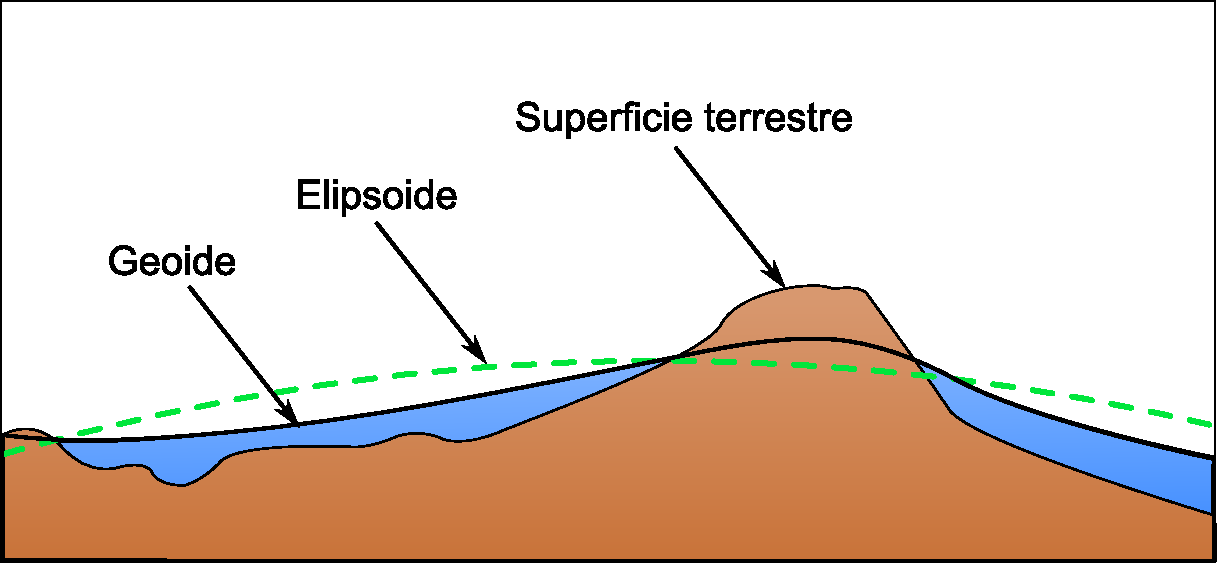
\includegraphics[width=.6\columnwidth]{Fundamentos_cartograficos/Tres_superficies.pdf}
\caption{\small Tres superficies fundamentales: superficie real de la Tierra, geoide y elipsoide (Adaptado de Wikipedia).}
\label{Fig:Tres_superficies} 
\end{figure}

En un elipsoide general, tanto la posici�n de su centro de gravedad como de su plano ecuatorial coinciden con los terrestres. Por el contrario, cuando el elipsoide es local, estas propiedades no han de cumplirse necesariamente, y el elipsoide a solas resulta insuficiente ya que carecemos de informaci�n sobre su posicionamiento con respecto a la superficie terrestre. 

Surge as� el concepto de \textbf{datum}, que es el conjunto formado por una superficie de referencia (el elipsoide) y un punto en el que <<enlazar>> este al geoide. Este punto se denomina \textbf{punto fundamental}, y en �l el elipsoide es tangente al geoide. La vertical al geoide y al elipsoide son id�nticas en el punto fundamental. 

Para un mismo elipsoide pueden utilizarse distintos puntos fundamentales, que dar�n lugar a distintos datum y a distintas coordenadas para un mismo punto.

\subsection{Sistemas de coordenadas}

Una vez hemos definido un modelo para definir la forma de la Tierra, podemos establecer un sistema de codificar cada una de las posiciones sobre su superficie y asignar a estas las correspondientes coordenadas. Para ello, encontramos dos opciones: utilizar los elementos de la \textbf{geometr�a esf�rica} y con estos definir el sistema de referencia, o utilizar la \emph{geometr�a plana}, para lo cual ser� necesario un mecanismo de \textbf{proyecci�n} de coordenadas que permita situar los elementos de la superficie del elipsoide sobre una superficie plana.

El sistema de \emph{coordenadas geogr�ficas} es un sistema de coordenadas esf�ricas mediante el cual un punto se localiza con dos valores angulares: \textbf{latitud}
y \textbf{longitud}. Las lineas de igual latitud o longitud se denominan \textbf{paralelos} y \textbf{meridianos} respectivamente.

Las coordenadas geogr�ficas resultan de gran utilidad, especialmente cuando se trabaja con grandes regiones. No obstante, no se trata de un sistema cartesiano, y tareas como la medici�n de �reas o distancias es mucho m�s complicada. Para poder crear cartograf�a y simplificar gran n�mero de operaciones posteriores, necesitamos coordenadas cartesianas. El proceso de asignar una coordenada plana a cada punto de la superficie de la Tierra (que no es plana) se conoce como \textbf{proyecci�n cartogr�fica}.

La superficie de la esfera no es \textbf{desarrollable}, es decir, no puede convertirse en un plano. Por ello, es necesario disponer de una metodolog�a para pasar puntos desde la superficie curva al plano, tal y como el que se muestra en la figura \ref{Fig:Proyeccion}.

\begin{figure}
\centering
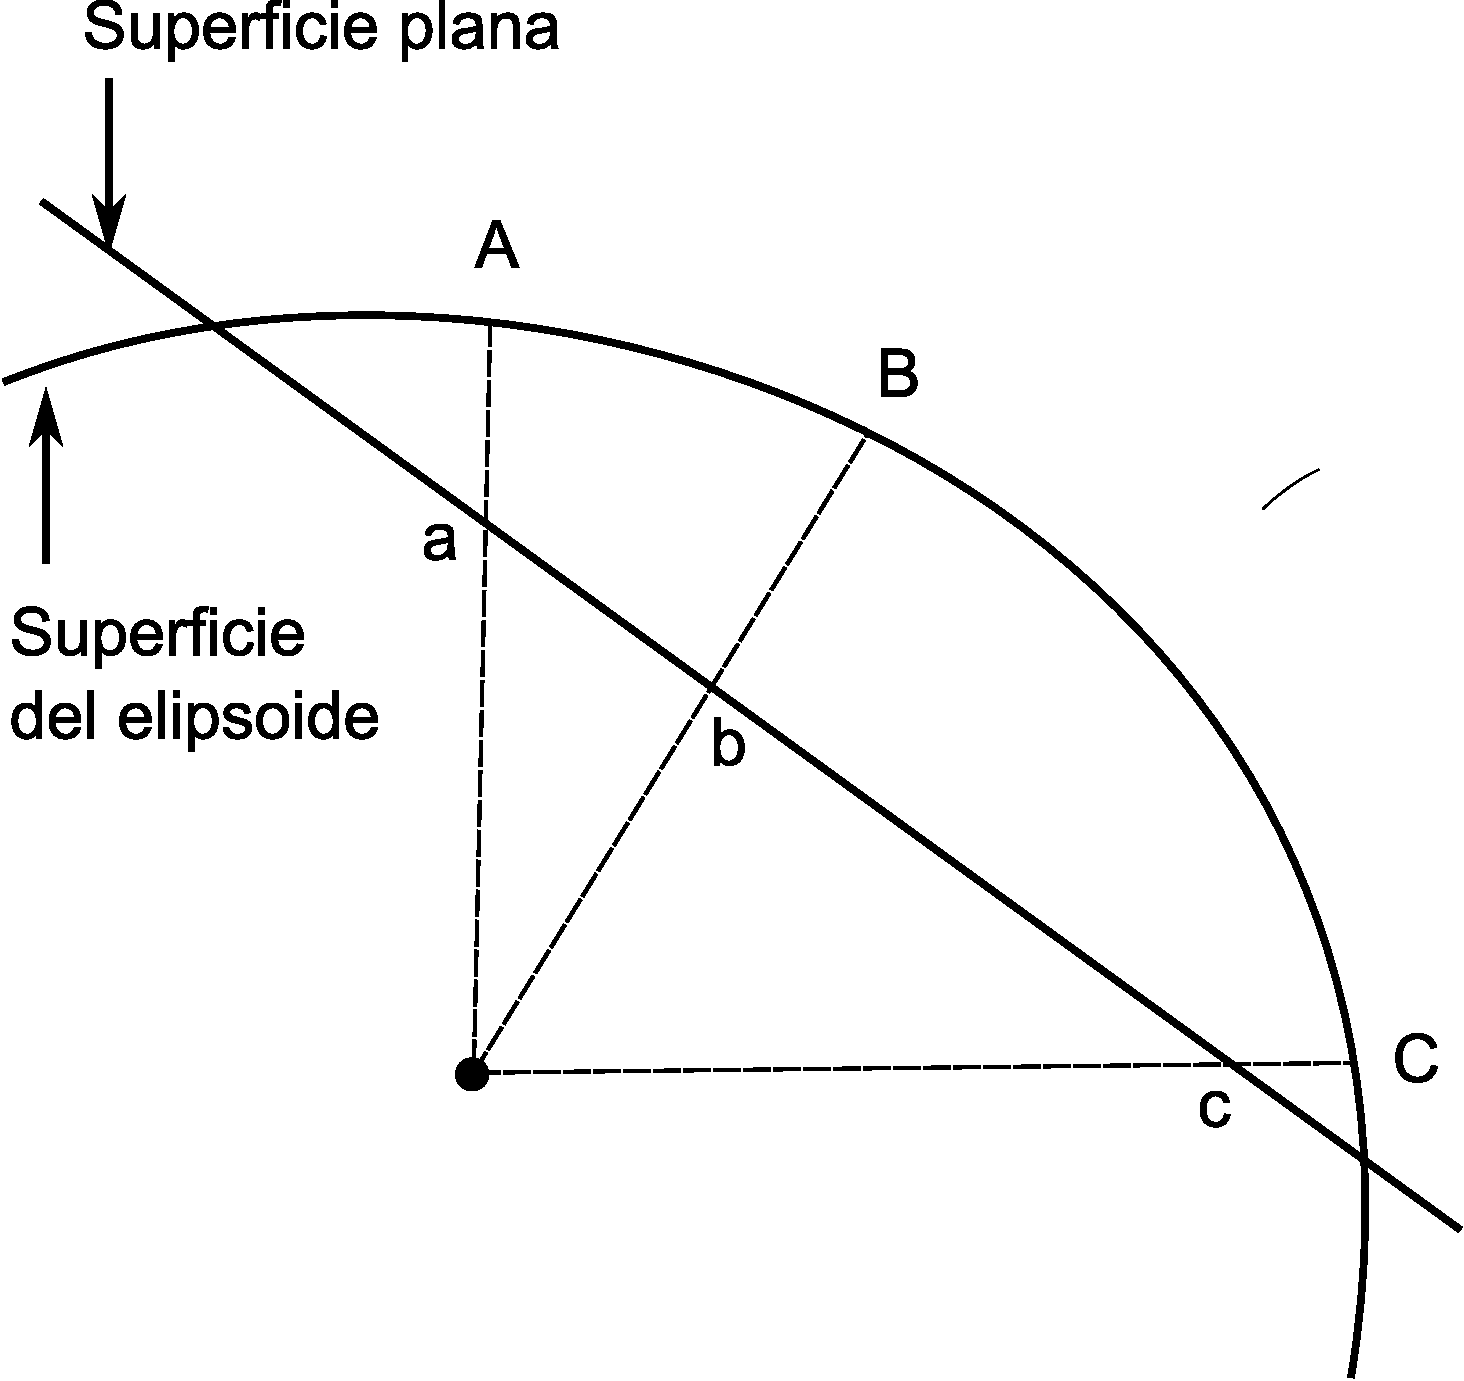
\includegraphics[width=.5\columnwidth]{Fundamentos_cartograficos/Proyeccion.pdf}
\caption{\small Esquema del concepto de proyecci�n. A los puntos $A, B$ y $C$ sobre la superficie del elipsoide se les asocian equivalentes $a, b$ y $c$ sobre un plano.}
\label{Fig:Proyeccion} 
\end{figure}


En el caso de la figura, los puntos se proyectan directamente sobre un plano. Otra opci�n es proyectarlos sobre una superficie tridimensional que, al contrario que la esfera, sea desarrollable. Las m�s habituales son el cilindro y el cono, que dan lugar a las \textbf{proyecciones c�nicas} y \textbf{cil�ndricas}.

Puede apreciarse en la figura que se producen distorsiones al realizar la proyecci�n. Por ejemplo, la distancia entre los puntos $A$ y $B$ no es igual a la existente entre los puntos $a$ y $b$. Con independencia de las caracter�sticas propias de la proyecci�n, siempre existen distorsiones, por ser la de la esfera una superficie no desarrollable. Estas distorsiones se conocen como \textbf{anamorfosis} . 


Seg�n las propiedades m�tricas que se conserven, las proyecciones pueden ser \textbf{equi�rea} (mantienen una escala constante), \textbf{conformes} (mantienen los �ngulos y la forma de los objetos) o \textbf{equidistantes} (mantienen las distancias).

La elecci�n de una u otra proyecci�n es funci�n de las necesidades concretas de cada caso de uso. 

En la actualidad, una de las proyecciones m�s extendidas en todos los �mbitos es la \textbf{proyecci�n universal transversa de Mercator}, la cual da lugar al \textbf{sistema de coordenadas UTM}. Este sistema no es simplemente una proyecci�n, sino un sistema completo para cartografiar la practica totalidad de la Tierra. Para ello, esta se divide en una serie de zonas rectangulares mediante una cuadricula y se aplica una proyecci�n y unos par�metros geod�sicos concretos a cada una de dichas zonas. En su forma actual, emplea un �nico elipsoide (WGS--84).

Con el sistema UTM, las coordenadas de un punto no se expresan como coordenadas terrestres absolutas, sino mediante la zona correspondiente y las coordenadas relativas a la zona UTM en la que nos encontremos.

La cuadricula UTM tiene un total de 60 husos numerados entre 1 y 60, cada uno de los cuales abarca una amplitud de 6\degree de longitud. El huso 1 se sit�a entre los 180\degree y 174\degree O, y la numeraci�n avanza hacia el Este. 

En latitud, cada huso se divide en 20 zonas, que van desde los 80\degree S hasta los 84\degree N. Estas se codifican con letras desde la C a la X, no utiliz�ndose las letras I y O por su similitud con los d�gitos 1 y 0. Cada zona abarca 8 grados de longitud, excepto la X que se prolonga unos 4 grados adicionales. 

Una zona UTM se localiza, por tanto, \textbf{con un n�mero y una letra}, y es en funci�n de la zona como posteriormente se dan las coordenadas que localizan un punto. Estas coordenadas se expresan en metros y expresan la distancia entre el punto y el origen de la zona UTM en concreto. El origen de la zona se sit�a en el punto de corte entre el meridiano central de la zona y el ecuador. 

Para evitar la aparici�n de n�meros negativos, se considera que el origen no tiene una coordenada X de 0 metros, sino de 500000, y una coordenada Y de 10000000 metros, lo cual hace que todas las coordenadas referidas a �l sean positivas.

\subsection{Transformaci�n y conversi�n de coordenadas}

Una situaci�n muy habitual en el trabajo con un SIG es disponer de cartograf�a en \textbf{varios sistemas de coordenadas}, o bien en un mismo sistema pero con par�metros diferentes (por ejemplo, diferente datum). Para poder emplear toda esa cartograf�a de forma conjunta, resulta necesario trabajar en un sistema �nico y bien definido, lo cual hace necesario convertir al menos una parte de ella. Cuando el datum es distinto en los sistemas de origen y destino, la \textbf{conversi�n de coordenadas} se conoce como \textbf{transformaci�n de coordenadas}.

Las operaciones de transformaci�n y conversi�n aparecen en los SIG como funcionalidades que permiten modificar los datos geogr�ficos, reemplazando sus coordenadas por coordenadas en otro sistema de coordenadas. Igualmente, aparecen como funcionalidades de representaci�n, permitiendo la conversi�n <<\textbf{al vuelo}>>, es decir, en tiempo real. En este caso, un dato en un sistema de coordenadas se puede representar en cualquier otro sin necesidad de una conversi�n previa, con lo que puede usarse conjuntamente con datos en un sistema de coordenadas distinto.

Para facilitar el uso de sistemas de referencia, existen proyectos de codificaci�n de estos, de forma que cada sistema existente puede identificarse de forma sencilla mediante un c�digo. El m�s extendido de estos es el sistema de codificaci�n \textbf{EPSG}.

\section{Conceptos cartogr�ficos b�sicos}
\label{Escala}

De entre los conceptos fundamentales de la cartograf�a que todo usuario de SIG ha de conocer, destaca el de \textbf{escala}. La escala  es la \textbf{relaci�n de tama�o} existente entre el mapa que se obtiene al desarrollar nuestra superficie de proyecci�n (de tama�o acorde con el objeto proyectado, esto es la Tierra) y el que finalmente manejamos, de tama�o m�s reducido. Conociendo esta relaci�n podemos conocer las verdaderas magnitudes de los elementos que vemos en el mapa, ya que podemos convertir las medidas hechas sobre el mapa en medidas reales. Es importante recordar que esas medidas no son tan <<reales>>, puesto que la propia proyecci�n las ha distorsionado ---lo cual no debe olvidarse---, pero s� que son medidas en la escala original del objeto cartografiado.

La escala se expresa habitualmente como un denominador que relaciona una distancia medida en un mapa y la distancia que esta medida representa en la realidad. Por ejemplo, una escala 1:50000 quiere decir que 1 cent�metro en un mapa equivale a 50000 cent�metros en la realidad, es decir a 500 metros. Este valor se conoce como \textbf{escala num�rica}.

Independientemente del tipo de proyecci�n, la escala es completamente cierta �nicamente en determinadas partes del mapa. En otros puntos de este, la escala var�a. La relaci�n entre la escala en esos puntos y la escala num�rica se conoce como \textbf{factor de escala}. 

Aunque tradicionalmente se entiende la escala como un concepto asociado a la representaci�n, los datos geogr�ficos tienen una escala inherente que no es funci�n de dicha representaci�n, sino del detalle con que han sido tomados. En este sentido es m�s conveniente entender la escala como un elemento relacionado con la \textbf{resoluci�n} de los datos, es decir, con el \textbf{tama�o m�nimo cartografiado}. Esta concepci�n no es en absoluto propia de los SIG, ya que deriva de las representaciones cl�sicas y los mapas impresos. Se sabe que el tama�o m�nimo que el ojo humano es capaz de diferenciar es del orden de 0,2 mm. Aplicando a este valor la escala a la que queremos crear un mapa, tendremos la m�nima distancia sobre el terreno que debe medirse. 

Es importante ser consciente de la limitaci�n que la escala considerada a la hora de la toma de datos (conocida como \textbf{escala operacional}) impone, especialmente en el contexto de un SIG. En un SIG, podemos aumentar el tama�o en pantalla de una cierta informaci�n geogr�fica, variando la escala de representaci�n (tambi�n conocida como \textbf{escala cartogr�fica}), pero ello no modifica la escala operacional. Por mucho que ampliemos no vamos a ver m�s detalles, ya que para ello ser�a necesario tomar m�s datos. 

Un tipo de datos particulares con los que se trabaja en un SIG, los datos \emph{r�ster}, tienen a su vez un par�metro de resoluci�n (el \textbf{tama�o de celda}) ligado a la escala. Veremos m�s al respecto en el cap�tulo \ref{Tipos_datos}.

\label{GeneralizacionCartografica}

Relacionado con el concepto de escala encontramos la denominada \textbf{generalizaci�n cartogr�fica}. Generalizar implicar expresar alguna idea o informaci�n de forma m�s resumida, de tal modo que esta sea comprensible y pueda aprovecharse de la mejor manera posible. La generalizaci�n es necesaria en un SIG para representar datos a una escala menor que su escala operacional, ya que a las limitaciones de la visi�n humana han de sumarse las limitaciones de resoluci�n que los dispositivos presentan. Por ejemplo, no tiene sentido representar el callejero de una ciudad a una escala peque�a como la que se utilizar�a para representar un mapa mundial, ya que cada peque�o punto de la pantalla contendr�a un gran n�mero de calles. Adem�s de obtener un resultado inservible, se consumir�an recursos en efectuar todos los c�lculos necesarios para producir esa representaci�n.

En ocasiones, el proceso de generalizaci�n es necesario por razones distintas a las anteriores, y requiere operaciones tambi�n distintas. Por ejemplo, podemos crear un mapa del mundo que contenga v�as de comunicaci�n, pero no todas, sino solo las principales autopistas de cada pa�s. En este caso, no vamos a encontrar problemas con distintas carreteras que se solapan en la representaci�n, ni tampoco un volumen excesivo de datos, pero debemos igualmente <<adaptar>> la representaci�n a la escala, es decir, efectuar alg�n tipo de generalizaci�n. En este caso, se representar�an las carreteras con un ancho mayor del real, ya que, de otro modo, no ser�an apenas visibles.

\begin{figure}
\centering
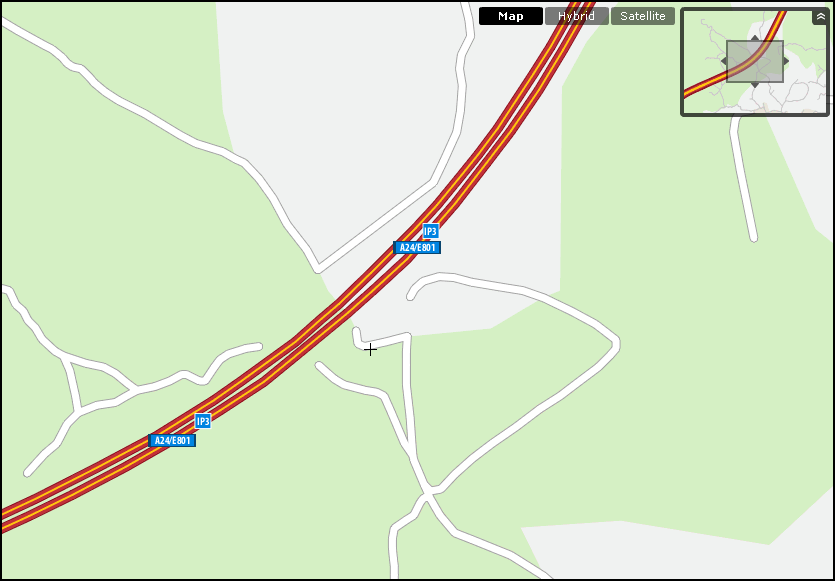
\includegraphics[width=.75\columnwidth]{Fundamentos_cartograficos/Generalizacion_agregacion.png}
\caption{\small Un ejemplo de generalizaci�n por agregaci�n. Dos carreteras pr�cticamente paralelas y unidas se representan como dos elementos en el mapa, pero en el localizador de la parte superior izquierda, a escala de menor detalle, se generalizan como una �nica (Tomado de Yahoo Maps).}
\label{Fig:Generalizacion_agregacion} 
\end{figure}

La generalizaci�n, por tanto, es un proceso que tiene como objetivo la producci�n de una imagen cartogr�fica \textbf{legible y expresiva}, reduciendo el contenido del mapa a aquello que sea posible y necesario representar. Para ello, se enfatiza lo que resulta de importancia y se suprime lo que carece de ella. 

Existen diversas operaciones que se emplean en el proceso de generalizaci�n. Algunas de las m�s relevantes son las \textbf{simplificaci�n} (representar un elemento menos complejo), la \textbf{agregaci�n} (representar varios elementos como uno solo ---Figura \ref{Fig:Generalizacion_agregacion}---), la \textbf{exageraci�n} (representar elementos con mayor tama�o del que les corresponde) y el \textbf{desplazamiento} (representar en una posici�n modificada, para garantizar la legibilidad). 




\label{Generalizacion_en_SIG}

En un SIG, la generalizaci�n puede incorporarse como parte de los propios mecanismos de representaci�n, aplic�ndose las transformaci�n correspondientes en tiempo real. A partir de un juego de datos, se elaboran las representaciones seg�n la escala a la que se est�n representando. Esta soluci�n tiene el inconveniente de producir resultados que no resultan �ptimos, por ser la generalizaci�n un proceso complejo y dif�cil de automatizar, y, sobre todo, el de consumir gran cantidad de recursos. La generalizaci�n en este caso tiene un objetivo cartogr�fico, pero en lugar de  hacer m�s fluido el trabajo con datos de gran volumen, lo hace m�s lento.

Una soluci�n alternativa y m�s adecuada de incorporar la generalizaci�n dentro de un SIG suele basarse en un enfoque multi--escalar (Figura \ref{Fig:SIG_multi_escala}), en el cual se maneja informaci�n de una misma zona de estudio a diferentes escalas, y se usa en cada momento aquella que resulte m�s conveniente. Si se trabajara con cartograf�a en papel, ser�a equivalente a tener varios mapas de una zona a diferentes escalas.

\begin{figure}
\centering
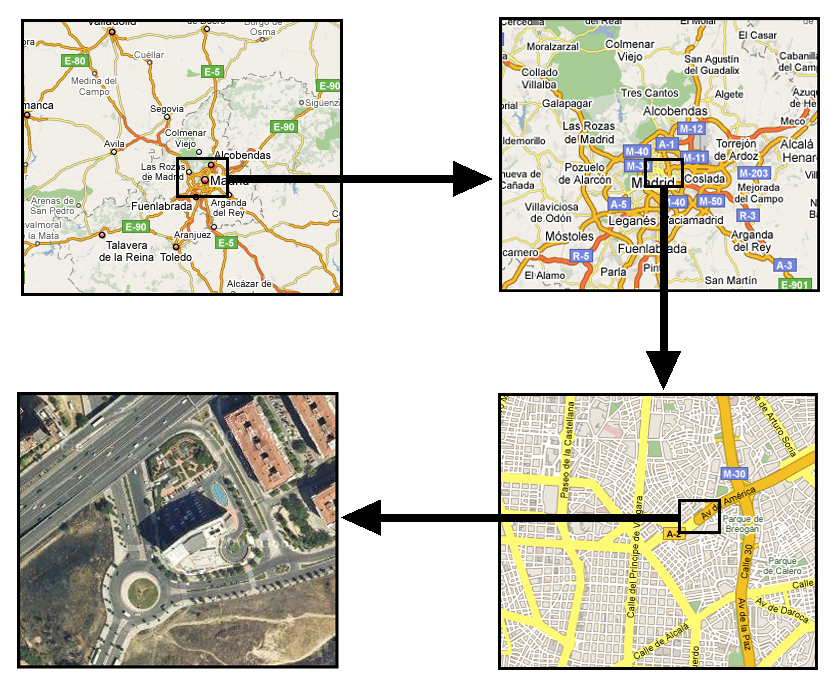
\includegraphics[width=\textwidth]{Fundamentos_cartograficos/SIG_multi_escala.png}
\caption{\small En un SIG es habitual manejar informaci�n a diferentes escalas. En funci�n de la escala de representaci�n, la informaci�n visualizada ser� una u otra.}
\label{Fig:SIG_multi_escala} 
\end{figure}


El concepto de \emph{capa},\index{Capa} que veremos en el cap�tulo \ref{Introduccion_datos} y que es vital para la idea actual de un SIG, permite este manejo simult�neo de informaci�n a distintas escalas.

En el caso de im�genes, este enfoque multi--escalar implica la creaci�n de las denominadas \textbf{pir�mides} (Figura \ref{Fig:Piramides}).


\begin{figure}
\centering
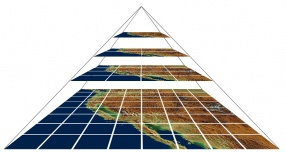
\includegraphics[width=.55\textwidth]{Fundamentos_cartograficos/Piramide.png}
\caption{\small Pir�mides de representaci�n con im�genes preparadas a distintas escalas (Fuente: OSGeo).}
\label{Fig:Piramides} 
\end{figure}

\pagestyle{empty}


%\pagestyle{empty}
\graphicspath{{Datos/}}


\chapter{El dato geogr�fico y su almacenamiento}
\label{Introduccion_datos}



De todos los subsistemas de un SIG, el correspondiente a los datos es el pilar fundamental que pone en marcha los restantes. Los datos son el combustible que alimenta el SIG. El subsistema de datos es, a su vez, el m�s interrelacionado, y est� conectado de forma inseparable a todos los restantes. 


\pagestyle{fancy}

\section{Datos \emph{vs} Informaci�n. Tipos de informaci�n.}

Existe una importante diferencia entre los conceptos de \textbf{datos} e \textbf{informaci�n}. Un SIG es un Sistema de \emph{Informaci�n} Geogr�fica, pero maneja \emph{datos} geogr�ficos, existiendo diferencias entre estos conceptos.

Entendemos como dato al simple conjunto de valores o elementos que utilizamos para representar algo. Por ejemplo, el c�digo 502132N es un dato. 

El dato anterior podemos interpretarlo como si fuera una referencia geogr�fica, y cuyo significado ser�a entonces una latitud, en particular 50\degree $21'$ $32''$ Norte. Si lo interpretamos como un c�digo que hace referencia a un documento de identificaci�n de una persona, la informaci�n que nos aporta es en ese caso completamente distinta. El dato ser�a el mismo, formado por seis d�gitos y una letra, pero la informaci�n que da es diferente, ya que lo entendemos e interpretamos de manera distinta.

La informaci�n es, por tanto, el resultado de un dato y una \textbf{interpretaci�n}, y el trabajo con datos es en muchos casos un proceso enfocado a obtener de estos toda la informaci�n posible. 

Comprender el significado y las diferencias entre datos e informaci�n permiten entender entre otras cosas que la relaci�n entre los vol�menes de ambos no es necesariamente constante. Por ejemplo, los datos 502132NORTE o CINCUENTA VEINTIUNO TREINTAYDOS NORTE son mayores en volumen que 502132N, pero recogen la misma informaci�n espacial que este (suponiendo que los interpretamos como datos de latitud). 

En la informaci�n geogr�fica se distinguen dos componentes: \textbf{espacial} y \textbf{tem�tica}. La componente espacial hace referencia a la posici�n dentro de un sistema de referencia establecido, y responde a la pregunta \emph{�d�nde?}. La componente tem�tica responde a la pregunta \emph{�qu�?}, y define la naturaleza del fen�meno que se produce en la localizaci�n indicada por la componente espacial.


Mientras que la componente espacial va a ser generalmente un valor num�rico, pues son de esa naturaleza los sistemas de coordenadas que permiten expresar una posici�n concreta en referencia a un marco dado, la componente tem�tica puede ser \textbf{num�rica} o \textbf{alfanum�rica} (texto). Una variable num�rica puede a su vez ser de cuatro tipos: \textbf{nominal, ordinal, intervalo} o \textbf{raz�n}.


El tipo de variable condiciona las operaciones que pueden realizarse con un dato geogr�fico en funci�n de c�mo sea su componente tem�tica. 

Un concepto a tener en cuenta en relaci�n con las componentes de la informaci�n geogr�fica es la \textbf{{dimensi�n}}. Los elementos que registramos pueden ir desde sencillos puntos (0D) hasta vol�menes tridimensionales (3D).

Las diferentes formas de representar y almacenar la informaci�n, que veremos m�s adelante en este capitulo, dependen del tipo de variable con que se trabaje.



\section{Divisi�n de la informaci�n. Capas}

En un SIG, la informaci�n espacial referida a una zona de estudio est� dividida en varios niveles, de tal forma que, pese a coincidir sobre un mismo emplazamiento, informaci�n sobre distintas variables se encuentra recogida de forma independiente. Es decir, en funci�n de la componente tem�tica se establecen distintos bloques de datos espaciales. Cada uno de estos bloques tem�ticos se conoce como \textbf{capa} (Figura \ref{Fig:Concepto_capa}). 

\begin{figure}[!hbt] 
\centering
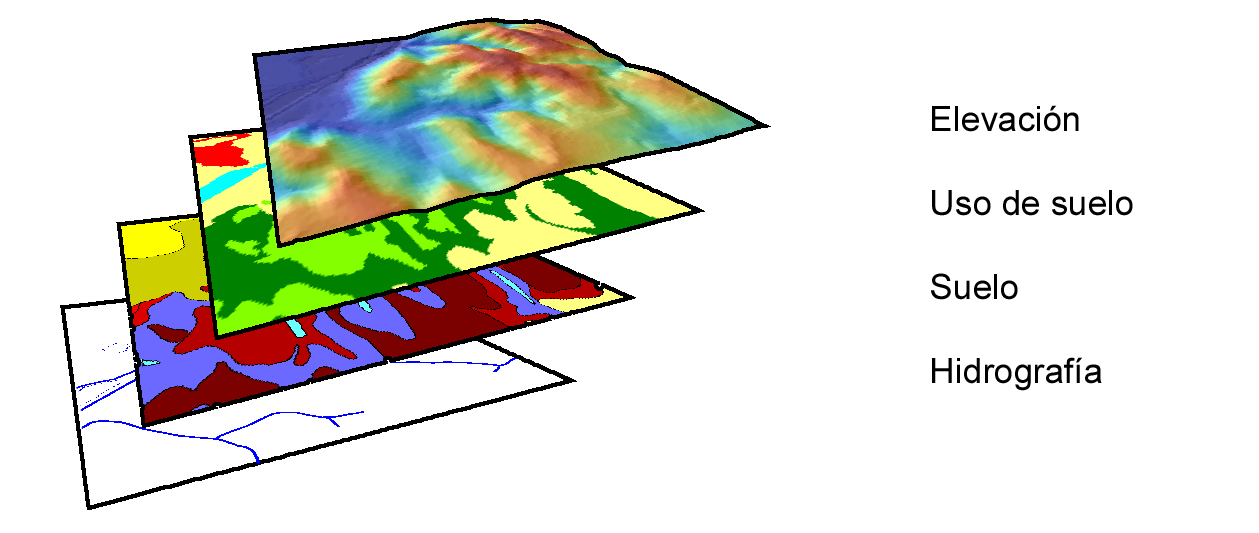
\includegraphics[width=.7\textwidth]{Introduccion_datos/Concepto_capa.png}
\caption{\small Concepto de \emph{capa} de informaci�n geogr�fica dentro de un SIG}
\label{Fig:Concepto_capa} 
\end{figure}

El concepto de capa es imprescindible para comprender todo SIG, y  favorece la correcta estructuraci�n de la informaci�n y el trabajo con ella. Toda la informaci�n geogr�fica con que trabajemos en un SIG va a ser en forma de capas. Cada una de ellas puede abrirse de forma independiente en un SIG y utilizarse por s� misma o en conjunto con otras.

Con la cartograf�a cl�sica, no es posible (o resulta dif�cil e impreciso) combinar distintos tipos de informaci�n, como por ejemplo la contenida en un mapa topogr�fico y la existente en un mapa de tipos de suelo y otro de vegetaci�n potencial. En el caso de un SIG, los distintos tipos de informaci�n se pueden combinar de forma sencilla y limpia, y no aparecen los mismos problemas

La relevancia del concepto de capa como elemento fundamental de un SIG es enorme, pues constituye el marco b�sico sobre el que se van a llevar a cabo gran parte de las operaciones. Por ejemplo, vimos en el apartado dedicado a la generalizaci�n cartogr�fica c�mo en un SIG podemos utilizar diferentes <<versiones>> de los datos correspondientes a una zona concreta, y representar una u otra de ellas en funci�n de la escala de trabajo. Estas versiones se almacenar�n como distintas capas. La capa es as� la unidad fundamental no solo en t�rminos de un �rea dada, sino tambi�n de una escala concreta, y permite una divisi�n de los datos �ptima a todos los efectos.


La separaci�n de la informaci�n en capas evita asimismo la redundancia de datos, ya que cada capa contiene un tipo de informaci�n concreto. En un mapa cl�sico se presentan siempre varias variables, algunas de ellas presentes con car�cter general, tales como nombres de ciudades principales o v�as m�s importantes de comunicaci�n. En un SIG, al encontrarse estas variables separadas en sus correspondientes capas, es el usuario quien las combina.

El trabajo con capas permite, por tanto, una estructura \textbf{m�s organizada} y una \textbf{mayor atomizaci�n} de los datos, con las consecuentes ventajas en el almacenamiento, manejo y funcionalidad que esto conlleva.


Adem�s de dividir la informaci�n geogr�fica en capas de acuerdo con su contenido, tambi�n dividimos esta con criterios puramente espaciales, <<cort�ndola>> en unidades menores que ocupen una regi�n de amplitud m�s reducida. Este es un procedimiento similar al que encontramos en un mapa impreso, ya que el territorio de un pa�s se encuentra cartografiado en diferentes \emph{hojas}. 

La principal cualidad de un SIG para integrar de forma transparente datos correspondientes a zonas distintas y formar un mosaico �nico es la \textbf{separaci�n que existe entre datos y visualizaci�n}. Los datos son la base de la visualizaci�n, pero en un SIG estos elementos conforman partes del sistema bien diferenciadas. Esto quiere decir que los datos se emplean para crear un resultado visual pero en s� mismos no contienen valores relativos a esa visualizaci�n.

De este modo, es posible combinar los datos y despu�s representarlos en su conjunto. Un proceso as� no puede realizarse con un mapa ya impreso, pues este contiene ya elementos de visualizaci�n e incluso componentes cartogr�ficos tales como una flecha indicando el Norte, una leyenda o una escala. Por ello, aunque puedan combinarse, realmente no se <<funde>> la informaci�n de cada uno de los mapas para conformar uno �nico. En un SIG, por el contrario, la visualizaci�n de cuatro o m�s bloques de datos puede ser id�ntica a la que obtendr�a si todos esos datos constituyeran un �nico bloque. 

\section{Modelos para almacenamiento de informaci�n geogr�fica}
\label{Tipos_datos}

El proceso de convertir un �rea geogr�fica y la informaci�n acerca de ella en un dato susceptible de ser incorporado a un SIG puede dividirse en tres fases:

\begin{itemize}
 \item Establecimiento de un \textbf{modelo geogr�fico}. Es decir, un modelo conceptual de la realidad geogr�fica y su comportamiento.
\item Establecimiento de un \textbf{modelo de representaci�n}. Es decir, una forma de recoger el anterior modelo conceptual y sus caracter�sticas propias, reduci�ndolo a una serie finita de elementos.
\item Establecimiento de un \textbf{modelo de almacenamiento}. Es decir, un esquema de c�mo almacenar los distintos elementos del modelo de representaci�n.
\end{itemize}
\index{Modelo!geogr�fico}\index{Modelo!de representacion}\index{Modelo!de almacenamiento}



Por su mayor importancia, nos centraremos en los modelos de representaci�n. Los modelos de representaci�n que se utilizan principalmente en un SIG son dos: \textbf{modelo raster} y \textbf{modelo vectorial}. Las capas que utilizan estos modelos se conocen como \textbf{capas raster} y \textbf{capas vectoriales}, y esta es la terminolog�a habitual en el �mbito de los SIG para referirse a la naturaleza de una determinada capa. 

\subsection{Modelo r�ster}

El modelo r�ster se basa en una \textbf{divisi�n sistem�tica} del espacio. Todo el espacio queda cubierto y caracterizado como un conjunto de unidades elementales, cada una de ellas con un valor asociado.  

Lo m�s habitual es una divisi�n en una malla de \textbf{celdas cuadradas} o rectangulares. Conociendo la orientaci�n de la malla y las dimensiones de cada una de las celdas, as� como las coordenadas de al menos una de ellas, es posible conocer las coordenadas del resto en virtud de su \textbf{estructura regular}. Con esto, conocemos los valores de la variable en todos los puntos del espacio cubierto por la capa. El \textbf{tama�o de celda} es un par�metro relacionado con la escala de trabajo de la capa, ya que define la resoluci�n de esta y est� en funci�n de la precisi�n con que se han tomado los datos correspondientes.


La figura \ref{Fig:Raster_closeup} muestra un ejemplo de una malla r�ster con valores de elevaci�n.

\begin{figure}[!hbt]   
\centering
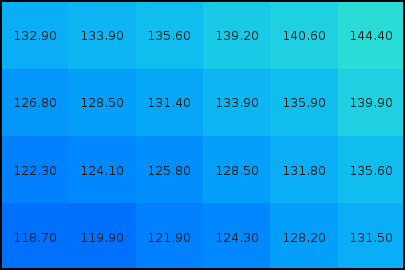
\includegraphics[width=.6\textwidth]{Tipos_datos/Raster_closeup.png}
\caption{\small Celdas de una malla r�ster con sus valores asociados.}
\label{Fig:Raster_closeup} 
\end{figure}

El n�mero de valores distintos recogidos para cada celda coincide con el n�mero de las denominadas \textbf{bandas}. Una banda contiene un �nico valor en una capa raster. Puede entenderse una capa raster de m�s de una banda como un conjunto de capas (cada banda ser�a una subcapa de ese conjunto), teniendo en todas ellas la malla de celdas las mismas caracter�sticas espaciales, y presentandose el conjunto como un �nico elemento. 

El ejemplo m�s claro de uso del modelo raster lo encontramos en las im�genes. Una imagen digital se compone de una malla de elementos (denominados \textbf{p�xeles}, cada uno de los cuales tiene un color asociado). El conjunto de estos p�xeles forman la imagen completa. Lo m�s habitual es que las im�genes contengan 3 bandas, correspondientes a las intensidades de los colores rojo, verde y azul, las cuales al combinarse permiten obtener el color de cada p�xel.

Otro uso habitual del modelo raster es en los denominados \textbf{Modelos Digitales de Elevaciones} (MDE), que recogen la topograf�a de un terreno. El modelo raster es el habitual de capa raster son las capas con modelos
De forma general, los valores de una capa r�ster, en cualquiera de sus bandas, son casi exclusivamente num�ricos, no estando los SIG preparados para manejar otro tipo de valores en la componente tem�tica de una capa r�ster. De esta forma, una capa raster puede equipararse al concepto matem�tico de una \textbf{matriz}, con las ventajas que ello supone para aplicar sobre ella herramientas matem�ticas a la hora de su an�lisis.




\subsection{Modelo vectorial}


El otro modelo principal de representaci�n es el modelo vectorial. En este modelo, no existen unidades fundamentales que dividen la zona recogida, sino que se recoge la variabilidad y caracter�sticas de esta mediante \textbf{entidades}, para cada una de las cuales dichas caracter�sticas son constantes. Las entidades se componen de \textbf{primitivas geom�tricas}, y estas pueden ser de tres tipos: \textbf{puntos, l�neas} y \textbf{pol�gonos}.

\begin{figure}[!hbt]   
\centering
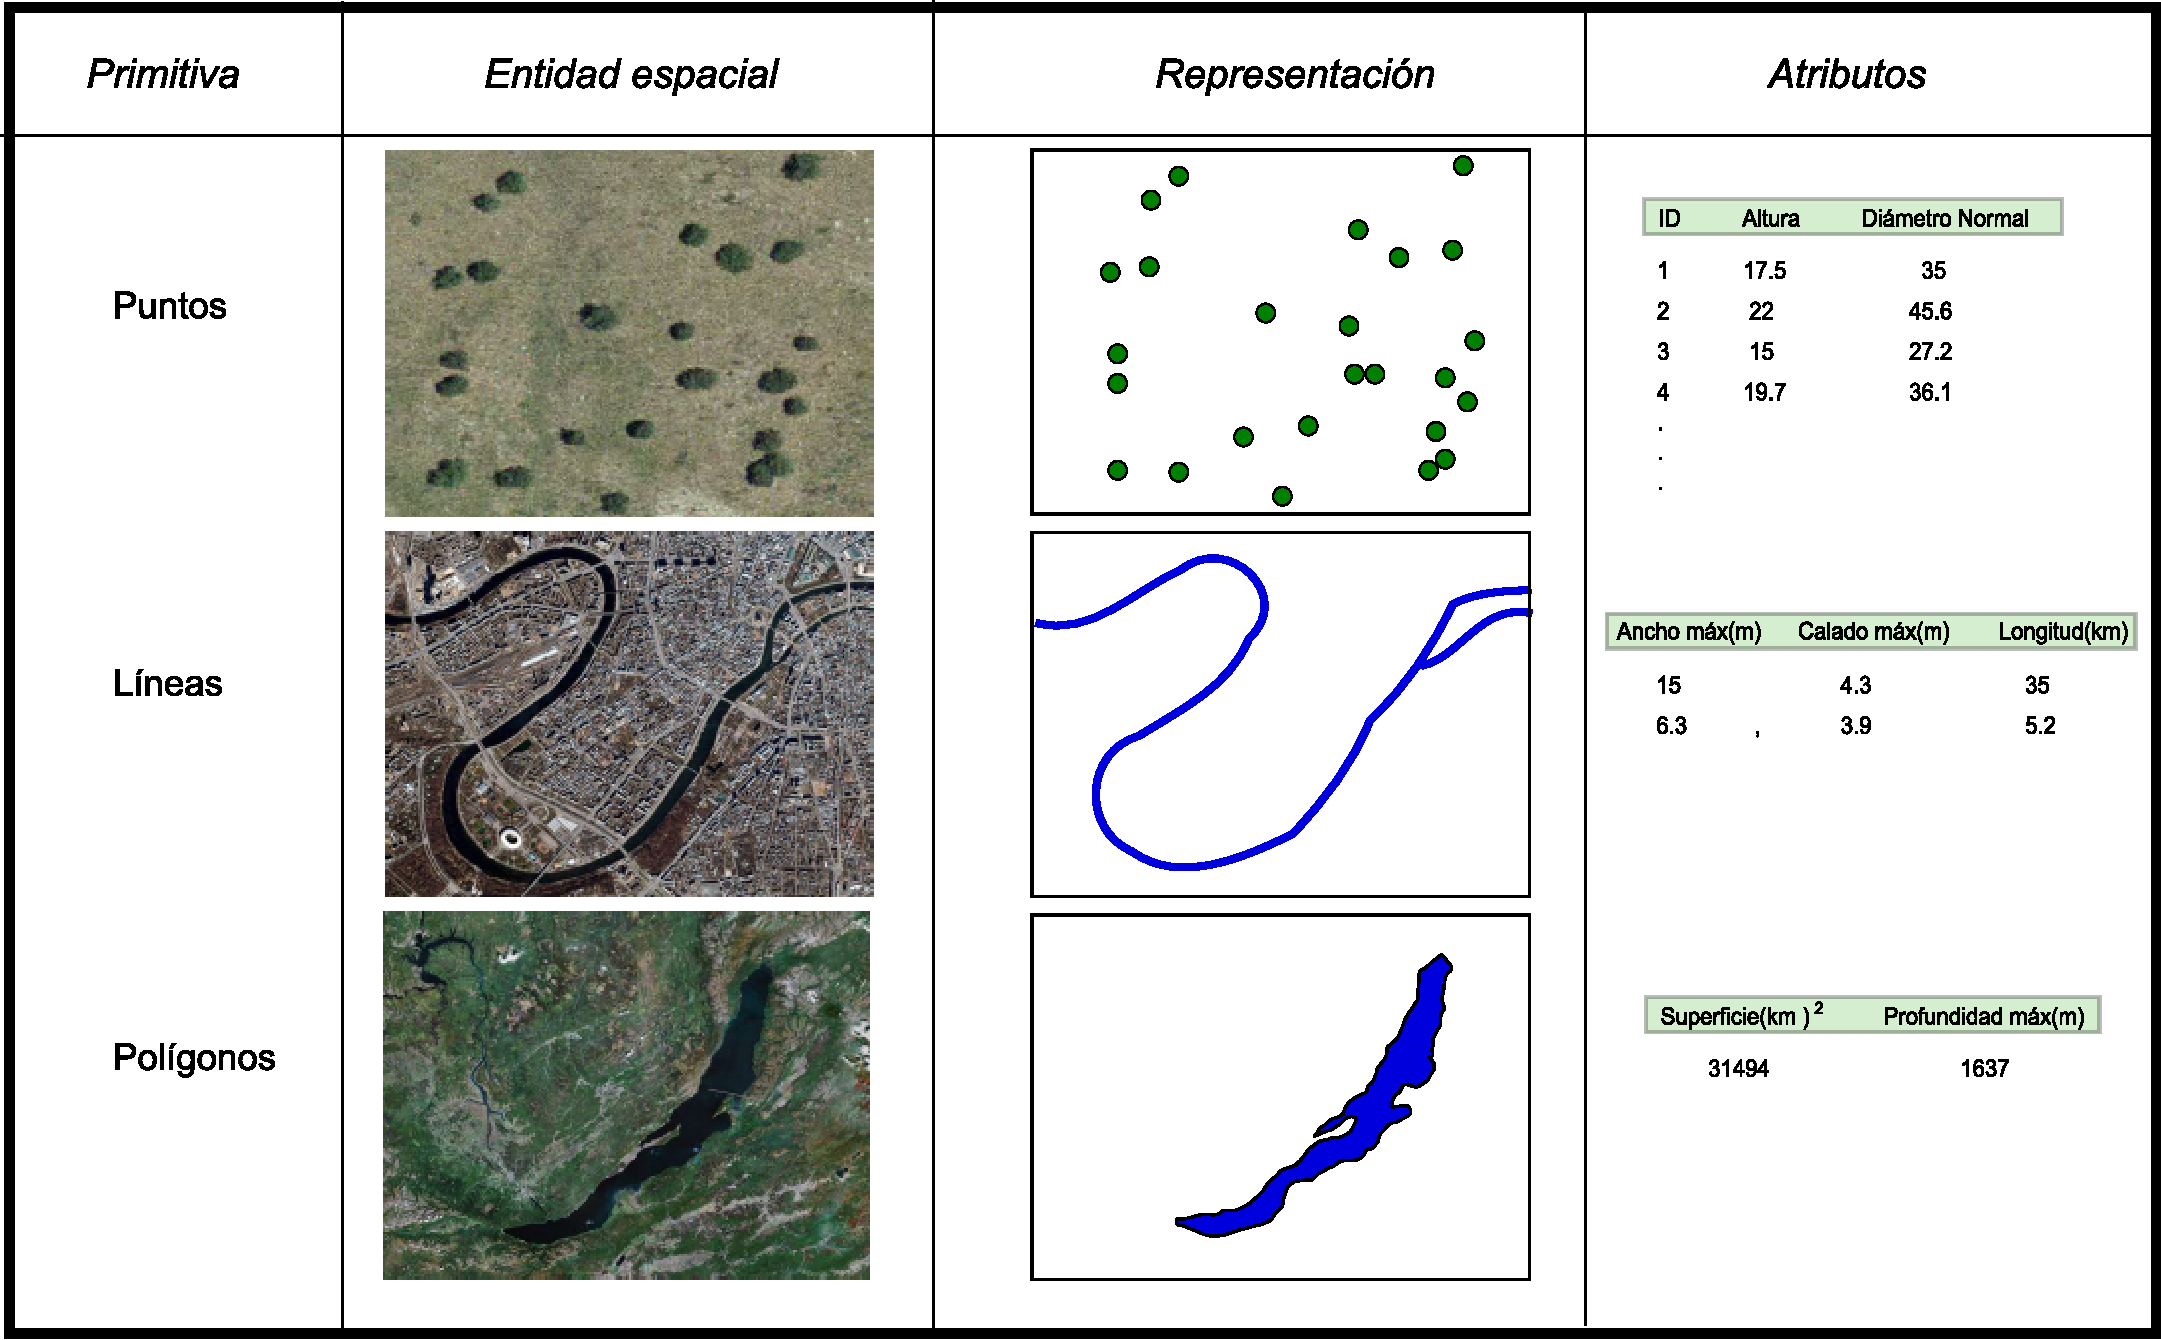
\includegraphics[width=\textwidth]{Tipos_datos/Primitivas_vectoriales.pdf}
\caption{\small Primitivas geom�tricas en el modelo de representaci�n vectorial y ejemplos particulares de cada una de ellas con atributos asociados}
\label{Fig:Primitivas_vectoriales} 
\end{figure}

Utilizando puntos, l�neas o pol�gonos, puede modelizarse el espacio geogr�fico si se asocia a estas geometr�as una serie de valores definitorios. Una entidad puede tener \textbf{varias primitivas}. Por ejemplo, en una capa de pa�ses, necesitar�amos varios conjuntos para representar Espa�a si queremos incluir tanto la peninsula como las islas que la forman. Todos estos pol�gonos constituyen una �nica entidad, ya que todos pertenecen al mismo pa�s y tendr�n el mismo conjunto de valores asociados.

A la hora de definir las formas geom�tricas b�sicas, todas ellas pueden en �ltima instancia \textbf{reducirse a puntos}. As�, las l�neas son un conjunto de puntos interconectados en un determinado orden, y los pol�gonos son l�neas cerradas, tambi�n expresables por tanto como una serie de puntos. Todo elemento del espacio geogr�fico queda definido, pues, por una serie de puntos que determinan sus propiedades espaciales y una serie de valores asociados.

Dentro de un SIG, una capa vectorial puede contener \textbf{un �nico tipo de primitiva}. As�, tenemos capas vectoriales de puntos, de l�neas y de pol�gonos, respectivamente. Una variable puede recogerse con varios tipos de primitivas (por ejemplo, puede indicarse una ciudad con un punto o con un pol�gono que delimite su per�metro), y la elecci�n de uno u otro tipo de geometr�a ha de ser funci�n del tipo de fen�meno que se pretende modelizar o la precisi�n necesaria, entre otros factores. 

La componente tem�tica en el modelo vectorial se establece mediante los denominados \textbf{atributos}, que suelen ser m�ltiples, a diferencia de lo que sucede en el modelo raster, donde lo habitual es tener un �nico valor para cada celda. Los atributos de una capa vectorial pueden contener informaci�n de cualqueir clase, siendo m�s vers�tiles que en el caso de las capas r�ster, donde ya vimos que se maneja �nicamente informaci�n num�rica. Por su estructura particular (series de atributos asociados a una entidad), la componente tem�tica en el modelo vectorial se presta especialmente a representarse en tablas y almacenarse en una \textbf{base de datos}, y puede analizarse independientemente de la componente espacial. 

Un elemento particular del modelo de representaci�n vectorial es la \textbf{topolog�a}.  Una capa vectorial contiene topolog�a si en ella se almacenan de alg�n modo las relaciones espaciales que existen entre sus elementos. Disponer de topolog�a en una capa vectorial es de gran importancia a la hora de llevar a cabo ciertos tipos de an�lisis, as� como procedimientos tales como la edici�n de los propios datos geogr�ficos. 

Aunque la mayor�a de operaciones con una capa vectorial pueden llevarse a cabo en ausencia de topolog�a, algunas de ellas como el \textbf{an�lisis de redes} no se pueden llevar a cabo sin topolog�a. Si pensamos en una capa de v�as sobre la que desarrollar ese an�lisis de redes, un mero conjunto de elementos geom�tricos (l�neas en este caso), no nos da informaci�n sobre los posibles enlaces entre las v�as que quedan representadas. Los puntos donde se cruzan dos v�as pueden ser cruces o rotondas (es decir, puede pasarse de una v�a a otra, existiendo conexi�n entre ellas), o bien pasos elevados o subterr�neos donde una de las v�as pasa por encima de la otra (y por tanto no existe comunicaci�n entre ambas). Las circunstancias son muy distintas en funci�n del tipo de cruce que exista, y por ello es imprescindible conocer esta informaci�n para efectuar un an�lisis de redes correcto (Figura \ref{Fig:Topologia_vias})

\begin{figure}[!hbt]   
\centering
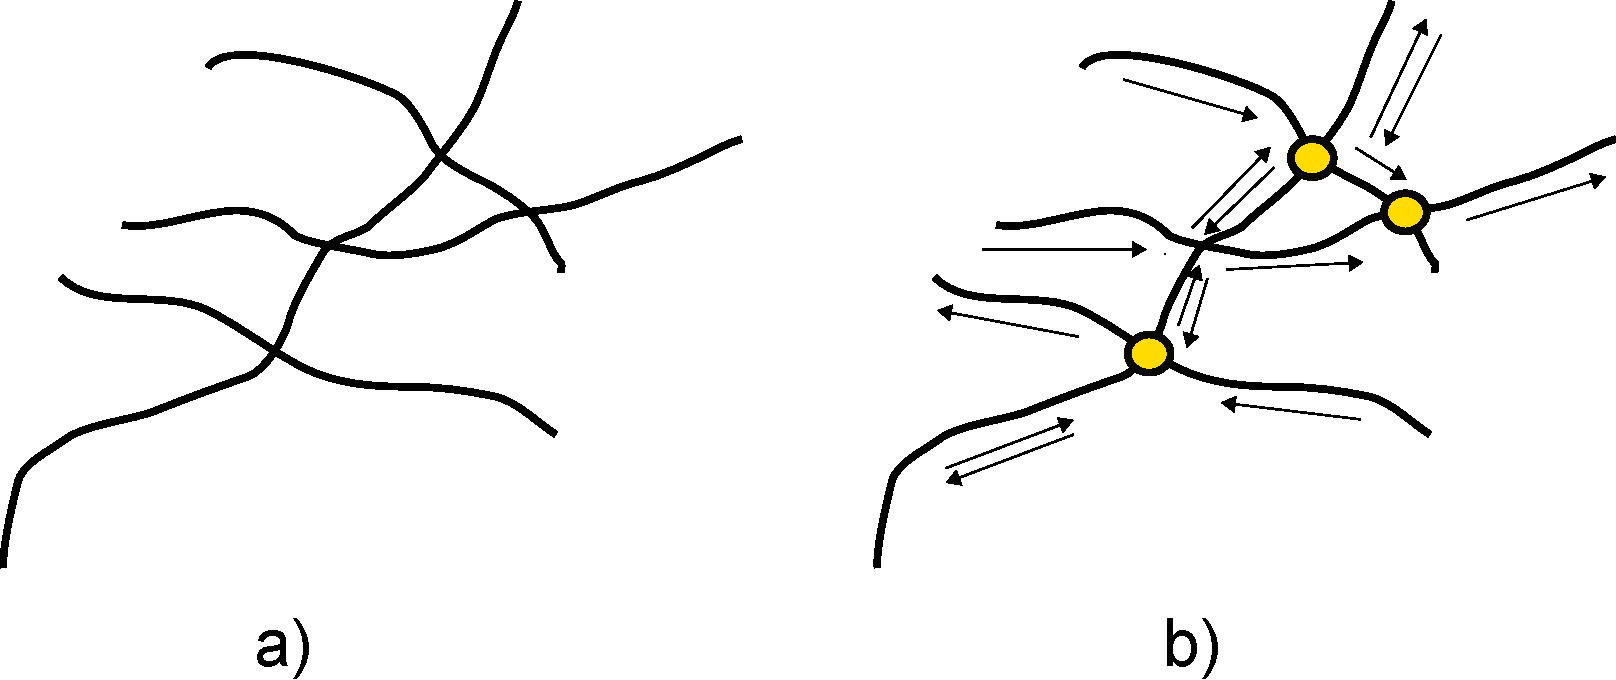
\includegraphics[width=.6\columnwidth]{Tipos_datos/Topologia_vias.pdf}
\caption{\small Capa de v�as de comunicaci�n sin topolog�a (a) o con ella (b). Los puntos en este segundo caso indican conexiones entre vias, y son una representaci�n visible de la topolog�a existente. }
\label{Fig:Topologia_vias} 
\end{figure}


El almacenamiento de entidades basado en una mera lista de coordenadas de cada entidad, sin topolog�a,  se conoce popularmente como \emph{spaghetti}, pues si pensamos en una capa de lineas sin topolog�a que se entrecruzan en el espacio, esta se asemejan en cierta forma a un ca�tico plato de \emph{spaguettis} sin orden ni relaci�n entre ellos.


\subsection{Raster \emph{vs} vectorial}


Tanto el modelo raster como el vectorial pueden emplearse para recoger \textbf{cualquier tipo de informaci�n}. La figura \ref{Fig:Esquemas_modelos_representacion} muestra un ejemplo de esto, representando una capa de v�as seg�n ambos modelos. Otro ejemplo para mostrar esto lo encontrarmos en las capas de elevaciones, que ya hemos visto que suelen recogerse en capas raster, en especial si se va a desarrollar sobre ellas alg�n tipo de an�lisis. No obstante, pueden recogerse tambi�n como una capa vectorial de puntos (este es una caso habitual si se obtienen los datos de un levantamiento topogr�fico), o bien como una capa de l�neas que contenga \textbf{curvas de nivel}, entre otras opciones.

\begin{figure}[!hbt]   
\centering
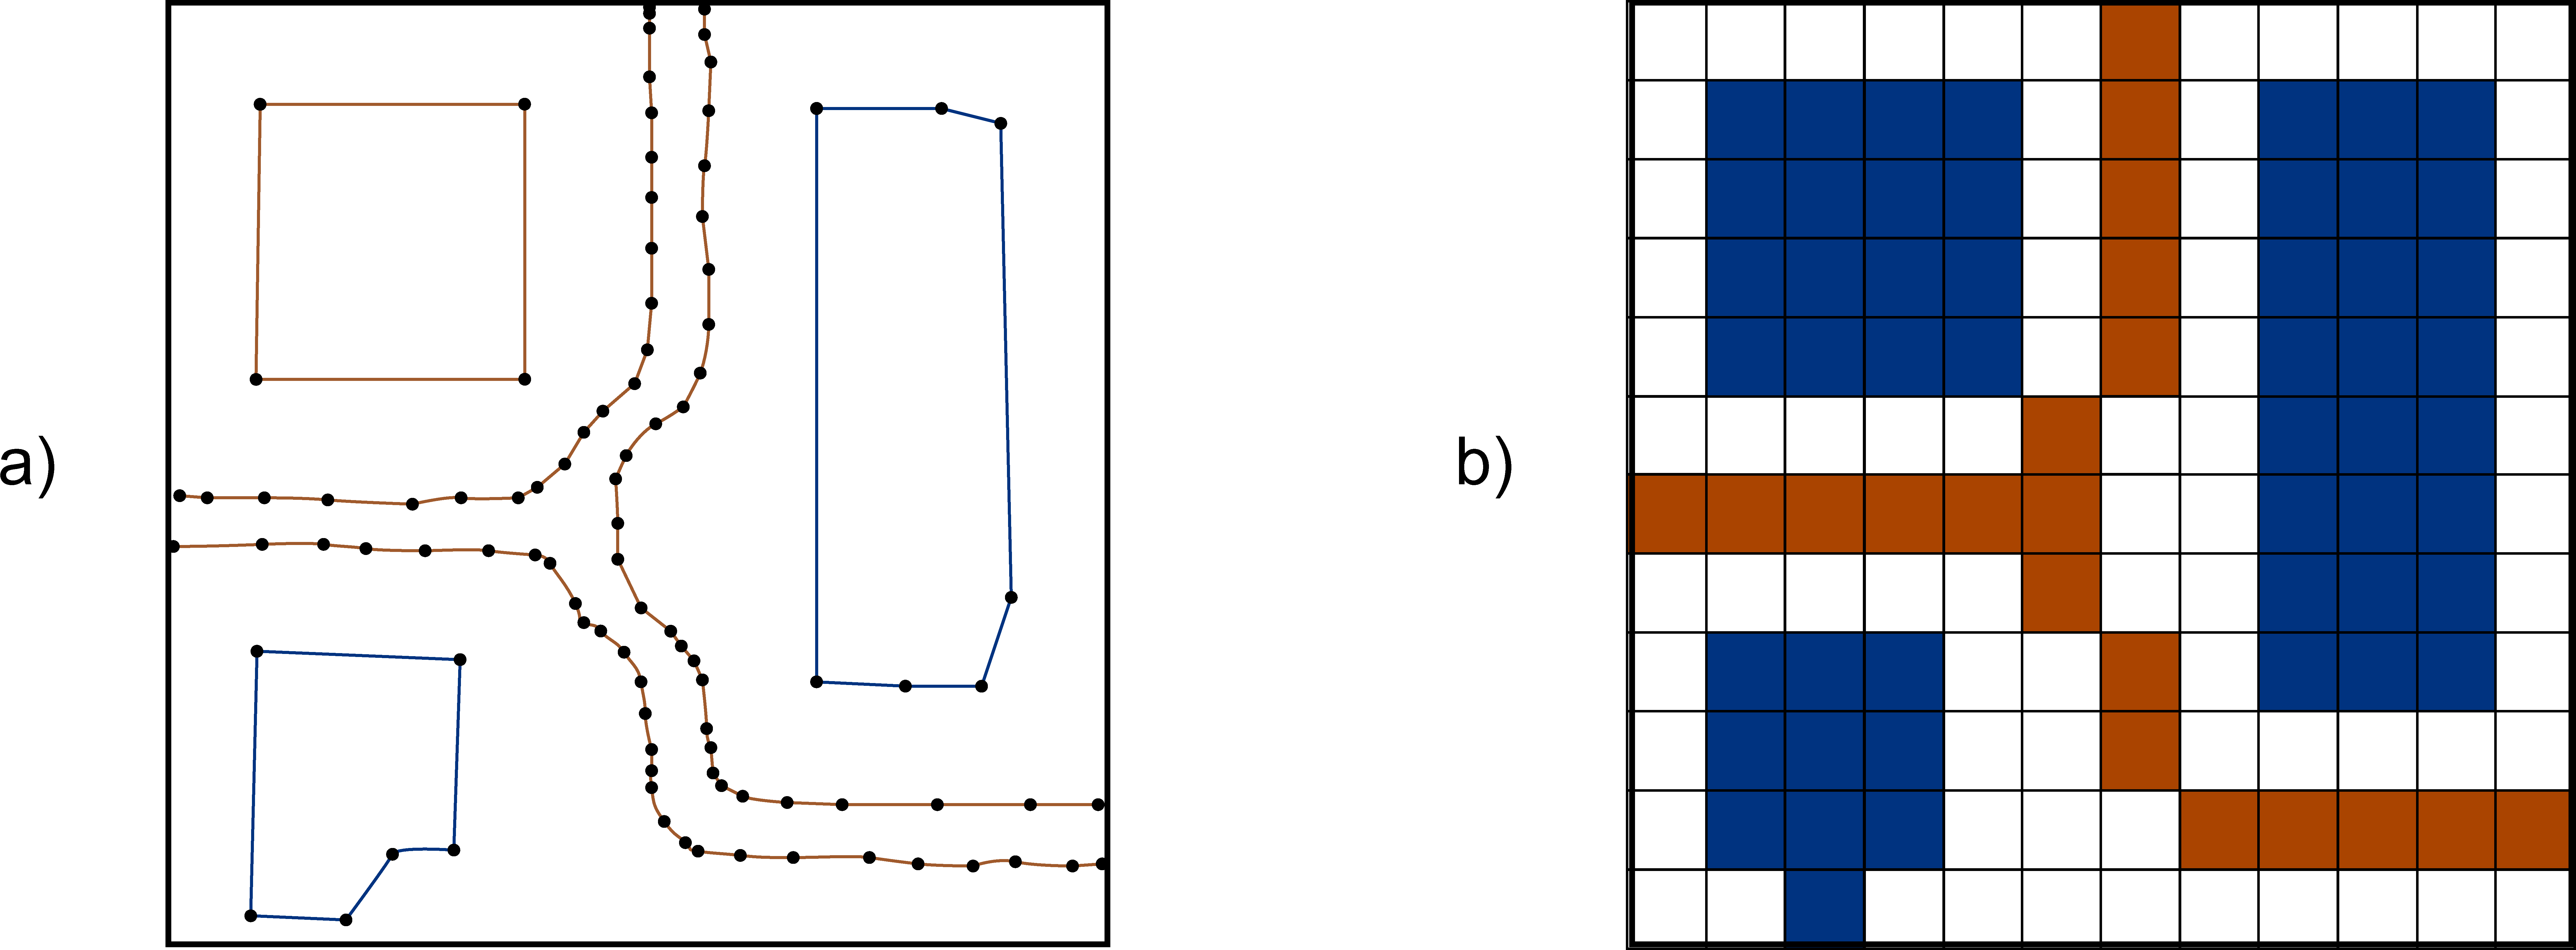
\includegraphics[width=.9\textwidth]{Tipos_datos/Esquemas_modelos_representacion.pdf}
\caption{\small Comparaci�n entre los esquemas del modelo de representaci�n vectorial (a) y r�ster (b).}
\label{Fig:Esquemas_modelos_representacion} 
\end{figure}


Resulta obvio que las diferencias entre los modelos r�ster y vectorial son muy notables, y que cada uno de ellos posee sus propias ventajas e inconvenientes. 
Algunos aspectos a los cuales puede atenderse para comparar uno y otro modelo son los siguientes:

\begin{itemize}
\item \textbf{Planteamiento}. El modelo r�ster hace m�s �nfasis en aquella caracter�stica del espacio que analizamos (\emph{qu�} y \emph{c�mo}), mientras que el modelo vectorial da prioridad a la localizaci�n de dicha caracter�stica (\emph{d�nde})
 \item \textbf{Precisi�n}. El modelo r�ster tiene su precisi�n limitada por el tama�o de celda. Las entidades menores que dicho tama�o de celda no pueden recogerse, y la variaci�n espacial que sucede dentro del espacio de la celda tampoco. 

Asimismo, existe una imprecisi�n en las formas. El detalle con el que puede recogerse la forma de una entidad geogr�fica seg�n el modelo vectorial es, en la pr�ctica, ilimitado, mientras que, como puede verse en la imagen \ref{Fig:Imprecision_raster}, el modelo r�ster restringe las formas a �ngulos rectos, ya que la unidad base es un cuadrado. 

\begin{figure}[!hbt]   
\centering
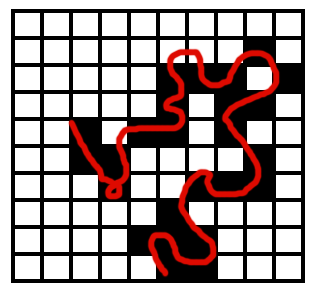
\includegraphics[width=.5\columnwidth]{Tipos_datos/Imprecision_raster.png}
\caption{\small Imprecisi�n de forma en el modelo de representaci�n r�ster. La divisi�n del espacio en unidades cuadradas impide la representaci�n fiel de entidades tales como curvas.}
\label{Fig:Imprecision_raster} 
\end{figure}

\item \textbf{Complejidad}. La regularidad y sistematicidad de las mallas r�ster hacen sencillo el implementar algoritmos de an�lisis, muy especialmente aquellos que implican el uso combinado de varias capas. Por el contrario, la irregularidad espacial de las capas vectoriales hace que la implementaci�n de los mismos algoritmos sea sumamente m�s compleja si se trabaja con estas capas.


\end{itemize}

No existe un modelo de representaci�n id�neo de forma global, sino que esta idoneidad depende de muchos factores, como por ejemplo:

\begin{itemize}
 \item \textbf{Tipo de variable o fen�meno a recoger}. Las variables \textbf{continuas} tales como la elevaci�n es m�s adecuado en general recogerlas en capas raster, para as� facilitar su an�lisis, mientras que las variables \textbf{discretas} es preferible almacenarlas como capas vectoriales.
\item \textbf{Tipo de an�lisis o tarea a realizar sobre dicha variable}. El uso que demos a una capa tem�tica condiciona en gran medida el modelo de datos id�neo. Por ejemplo, en el caso de una capa de elevaciones, su an�lisis se lleva mejor a cabo si esta informaci�n est� recogida seg�n el modelo r�ster. Sin embargo, si el objetivo principal es la visualizaci�n de esa elevaci�n en conjunto con otras variables, unas curvas de nivel pueden resultar m�s adecuadas, ya que, entre otras cosas, no interfieren tanto con otros elementos a la hora de dise�ar un mapa con todas esas variables.
\item \textbf{Contexto de trabajo}. Por ejemplo, si queremos trabajar con im�genes, esto nos condiciona al empleo de datos r�ster, ya que resulta mucho m�s sencillo combinarlos con las im�genes, las cuales siempre se presentan como capas r�ster. 
\end{itemize}


Existen procedimientos para \textbf{convertir} entre los formatos r�ster y vectorial, de forma que el disponer de datos en un modelo de representaci�n particular no implica que debamos desarrollar nuestro trabajo sobre dichos datos directamente, sino que podemos efectuar previamente una conversi�n. Los cap�tulos \ref{Creacion_capas_raster} y \ref{Creacion_capas_vectoriales} tratan estos temas en profundidad.




\pagestyle{empty}
%
\chapter{Modelos para la informaci�n geogr�fica}
\label{Tipos_datos}

 

\bigskip

\begin{intro}
La realidad geogr�fica debe recogerse en un formato que pueda ser entendido por el ordenador y as� susceptible de emplearse dentro de un SIG. En este cap�tulo se mostrar�n los enfoques conceptuales y pr�cticos m�s frecuentes para llevar esto a cabo, que a su vez son los responsables indirectos de las arquitecturas subyacentes en los SIG. Para ello, se estudiar�n los distintos tipos de informaci�n con los que trabajamos en un SIG y las formas m�s adecuadas de entender, interpretar y manejar esta.
\end{intro}

\section{Introducci�n}
\pagestyle{fancy}

Los datos son, como ya sabemos, una parte imprescindible del SIG, ya que sin ellos las aplicaciones SIG y los restantes elementos que se encuentran en torno a estas no tienen utilidad alguna. Necesitamos conocer el �rea geogr�fica que estudiamos en un SIG (es decir, tener datos sobre ella), para as� poder proceder a dicho estudio. 

No obstante, convertir ese �rea geogr�fica y la informaci�n acerca de ella en un dato susceptible de ser incorporado a un SIG no resulta una tarea sencilla. Desde los or�genes de los SIG, una de las preocupaciones principales ha sido la de representar de la mejor manera posible toda la informaci�n que podemos extraer de una zona geogr�fica dada, de tal modo que pueda almacenarse y analizarse en el entorno de un SIG. Este proceso de representaci�n, que ya desde el inicio planteaba problemas a los creadores de los primeros SIG, ha sido el responsable en gran medida de la arquitectura y forma de los SIG actuales, y a �l se debe en buena parte el desarrollo que han experimentado tanto los SIG en s� como las disciplinas afines.

Describir los enfoques te�ricos existentes para convertir la realidad relativa a una variable dada en una capa que la contenga de la forma m�s precisa posible y pueda ser empleada en un SIG es el objeto de este cap�tulo. Este proceso implica la construcci�n de un modelo (el dato geogr�fico), que representa la realidad y puede servir para conocer esta en profundidad a trav�s de an�lisis que no se llevan a cabo sobre dicha realidad, sino sobre el modelo en s�.

El problema principal reside en el hecho de que el detalle real que encontramos en la naturaleza es pr�cticamente infinito, mientras que la representaci�n y almacenamiento de esa realidad es finita. Se hace necesario extraer una serie de elementos y valores caracter�sticos, los cuales en ultima instancia se recoger�n como valores num�ricos dentro del SIG (pues son estos los que maneja un ordenador), y podr�n interpretarse como el anteriormente citado modelo. El camino que lleva desde la realidad hasta ese conjunto de meros valores num�ricos pasa por tres niveles:

\begin{itemize}
 \item Establecimiento de un \textbf{modelo geogr�fico}. Es decir, un modelo conceptual de la realidad geogr�fica y su comportamiento.
\item Establecimiento de un \textbf{modelo de representaci�n}. Es decir, una forma de recoger el anterior modelo conceptual y sus caracter�sticas propias, reduci�ndolo a una serie finita de elementos.
\item Establecimiento de un \textbf{modelo de almacenamiento}. Es decir, un esquema de c�mo almacenar los distintos elementos del modelo de representaci�n.
\end{itemize}
\index{Modelo!geogr�fico}\index{Modelo!de representacion}\index{Modelo!de almacenamiento}
El modelo geogr�fico es un ente puramente conceptual (de alto nivel), mientras que el de almacenamiento es m�s un concepto t�cnico inherente a la naturaleza inform�tica del SIG (de bajo nivel)

\section{Modelos geogr�ficos}

El primer paso hacia la creaci�n del dato geogr�fico implica el establecimiento de un modelo conceptual relativo a c�mo se ha de interpretar la realidad geogr�fica. Se trata de conceptualizar el espacio estudiado, la variable tratada y la variaci�n de esta a lo largo del espacio. Este modelo geogr�fico es un esquema mental que constituye una forma particular de entender el hecho geogr�fico en s�, pero que todav�a no incorpora elementos relativos a su representaci�n o almacenamiento.

Existen muchos modelos geogr�ficos distintos, entre los cuales cabe destacar dos de ellos \cite{Couclelis1992Springer}:

\begin{itemize}
 \item Campos
\item Entidades discretas
\end{itemize}

\index{Campos (modelo geogr�fico)}\index{Entidades!discretas}
\subsection{Campos}

Un campo es un modelo de variaci�n dentro de un marco n--dimensional, en el cual en cada punto dentro de dicho marco se tiene un valor de la variable estudiada. En su concepto matem�tico, un campo es una funci�n de la forma $\varphi:\mathbf{R}^n\rightarrow \mathbf{R}^m$, esto es, una funci�n que  asocia cada punto de un espacio vectorial con otro en un espacio vectorial distinto.

En el caso m�s habitual, $m=1$, es decir, que a cada punto del espacio vectorial origen se le asocia un �nico valor escalar. Se tiene as� lo que se denomina un \emph{campo escalar}. La mayor�a de las variables que se emplean en un SIG necesitan un �nico valor para describirse (pi�nsese en variables como la elevaci�n, la temperatura o la presi�n atmosf�rica, que solo requieren de un n�mero para expresarse), por lo que los campos escalares son los m�s habituales en el �mbito geogr�fico. 

\index{Campo!escalar}\index{Campos!vectorial} \index{Vectorial!campo}
No obstante, tambi�n encontramos los denominados \emph{campos vectoriales}\footnote{El empleo del t�rmino \emph{vectorial} para calificar a los campos vectoriales o los espacios vectoriales no debe confundirse con el modelo de representaci�n vectorial que veremos m�s adelante en este cap�tulo. En el caso de campos y espacio, se trata de la terminolog�a est�ndar del �mbito matem�tico, mientras que en el modelo de representaci�n vectorial es una terminolog�a propia de los Sistemas de Informaci�n Geogr�fica.}, en el cual el espacio vectorial de destino es multidimensional. Por ejemplo, para definir el movimiento del viento en un punto geogr�fico no basta con un �nico valor, sino dos: la velocidad y la direcci�n en la que sopla dicho viento. Dentro de un SIG, es habitual recoger los campos vectoriales como un conjunto de varios campos escalares, cada uno de ellos en una capa distinta. As�, se tendr�a una capa con la direcci�n y otra con la velocidad, ambas magnitudes escalares. Operando de esta manera, la soluci�n no es �nica, ya que el vector resultante puede definirse mediante su m�dulo y direcci�n (como en el caso anterior), pero tambi�n por sus propias coordenadas en la base del espacio vectorial destino (en el caso anterior, las componentes $x$ e $y$ del vector que indica el movimiento del viento).

\index{Espacio!vectorial}\index{Vectorial!espacio}

El espacio vectorial de origen puede ser bidimensional, es decir, una funci�n de la forma $f(x,y)$, representando $x$ e $y$ las coordenadas geogr�ficas. Este es el caso habitual en las capas que se emplean en un SIG, donde las variables que estudiamos adquieren uno u otro valor en funci�n de su posici�n dentro de un sistema coordenado de referencia.

Puede a�adirse una tercera dimensi�n, de tal modo que los valores dependan no solo de la posici�n sino igualmente de la elevaci�n. Se tendr�a una funci�n de la forma $f(x,y,z)$. Para el caso, por ejemplo, de la temperatura del aire, esta depende no solo de la localizaci�n, sino tambi�n de la altura. Otro ejemplo puede ser el porcentaje de arena en el suelo, que depende de la localizaci�n pero tambi�n de la profundidad.

Igualmente, aunque en general es poco habitual en el marco de los SIG, puede a�adirse la variable tiempo, teni�ndose funciones de la forma $f(x,y,t)$ o $f(x,y,z,t)$\index{Tiempo}

Por definici�n, un campo es continuo\index{Continuidad}, ya que todos los puntos tienen un valor asociado. De igual modo, este valor es �nico, y no existe un elemento del espacio vectorial de partida que tenga asociados varios elementos del de destino, sean estos escalares o vectores.

Por su propia naturaleza los campos son ideales para modelizar variables que var�an de forma continua en el espacio, entre ellas la practica totalidad de variables f�sicas del medio, tales como temperatura del aire, presi�n atmosf�rica, elevaci�n, etc.

Los campos se asocian con las denominadas \emph{coberturas}, termino este m�s empleado en el �mbito SIG. En una cobertura existe un valor �nico para todos los puntos de una regi�n dada.\index{Cobertura}

\subsection{Entidades discretas}

A diferencia de los campos, el modelo de entidades discretas no asocia a cada punto geogr�fico un valor, sino que concibe un entorno geogr�fico como un espacio vac�o sobre el que se sit�an distintos elementos (entidades) que lo van rellenando. Cada una de dichas entidades posee unas caracter�sticas propias, constantes para toda ellas, que son las que conferir�n sus propiedades particulares a los puntos que se sit�en en su interior.

Un punto puede no pertenecer a ninguna entidad, o bien a varias de ellas, seg�n sea la disposici�n de estas. Para un espacio dado, las entidades pueden ser todos aquellos elementos geom�tricos existentes en el mismo, tales como puntos, l�neas, pol�gonos o, en el caso de ser dicho espacio de dimensi�n mayor que dos, tambi�n vol�menes.

Es f�cil ver que el modelo de entidades discretas no es tan adecuado como los campos para conceptualizar variables continuas, ya que la continuidad de estas es opuesta al esquema discreto planteado. No obstante, otras variables no continuas se modelizan mejor mediante entidades discretas, ya que la forma en que se presentan coincide en cierta medida con dichas entidades como unidades m�nimas. 

La presencia de v�as de comunicaci�n, por ejemplo, se puede asimilar perfectamente a este modelo. Se tiene un espacio vac�o (sin v�as), en el cual se disponen los distintos viales en una serie de localizaciones concretas. Hay puntos que no estar�n afectados por ninguna entidad, mientras que otros (los situados en las intersecciones) lo est�n por varias de ellas.

Las variables de tipo nominal y alfanum�rico ---las cuales no son, como vimos, continuas--- tales como el tipo de suelo en un punto o el n�mero de parcela catastral al que pertenece dicho punto, tambi�n se adaptan bien al modelo de entidades discretas.
\index{Nominal}

Otra diferencia entre los campos y las entidades discretas es que estas �ltimas son en general m�s sencillas de comprender como concepto fuera de un �mbito t�cnico. Los campos son conceptos matem�ticos que requieren un mayor grado de abstracci�n, y para la mayor�a de la gente no resultan tan claros. Como algunos apuntan \cite{NCGIA}, el lenguaje habitual contiene un numero mayor de expresiones y recursos para describir la realidad geogr�fica en base a entidades discretas que en base a campos o conceptos abstractos similares.

\section{Modelos de representaci�n}

Los modelos geogr�ficos nos ofrecen una concepci�n particular del espacio geogr�fico y sus atributos. En base a ellos, el siguiente paso es reducir las propiedades de dichos modelos a un conjunto finito de elementos, de tal modo que el registro de dichos elementos sirva para almacenar la realidad que los modelos geogr�ficos describen. Para ello, empleamos los \emph{modelos de representaci�n}, tambi�n denominados \emph{modelos de datos}.

\index{Modelos!de datos}\index{Modelos!de representacion}\index{Datos!modelos de}

Antes de entrar a describir los distintos modelos de representaci�n, veamos algunos ejemplos que nos presentar�n casos particulares de estos modelos, aclarando sus diferencias antes de proceder a una definici�n m�s detallada. En la figura \ref{Fig:MDE_modelos_representacion} pueden verse distintas formas de representar la elevaci�n de una zona, la cual, como ya sabemos, es una variable continua y puede concebirse mediante un campo escalar. Por el contrario, la red viaria se adapta mejor a un modelo de entidades discretas, y se muestran en la figura \ref{Fig:Vias_modelos_representacion} sendas representaciones de esta variable seg�n distintos modelos de datos. Mediante los ejemplos de estas figuras presentaremos los modelos de datos principales, as� como su relaci�n con los modelos conceptuales estudiados en el punto anterior.

\index{Modelo Digital de Elevaciones}

\begin{figure}[!hbt]   
\centering
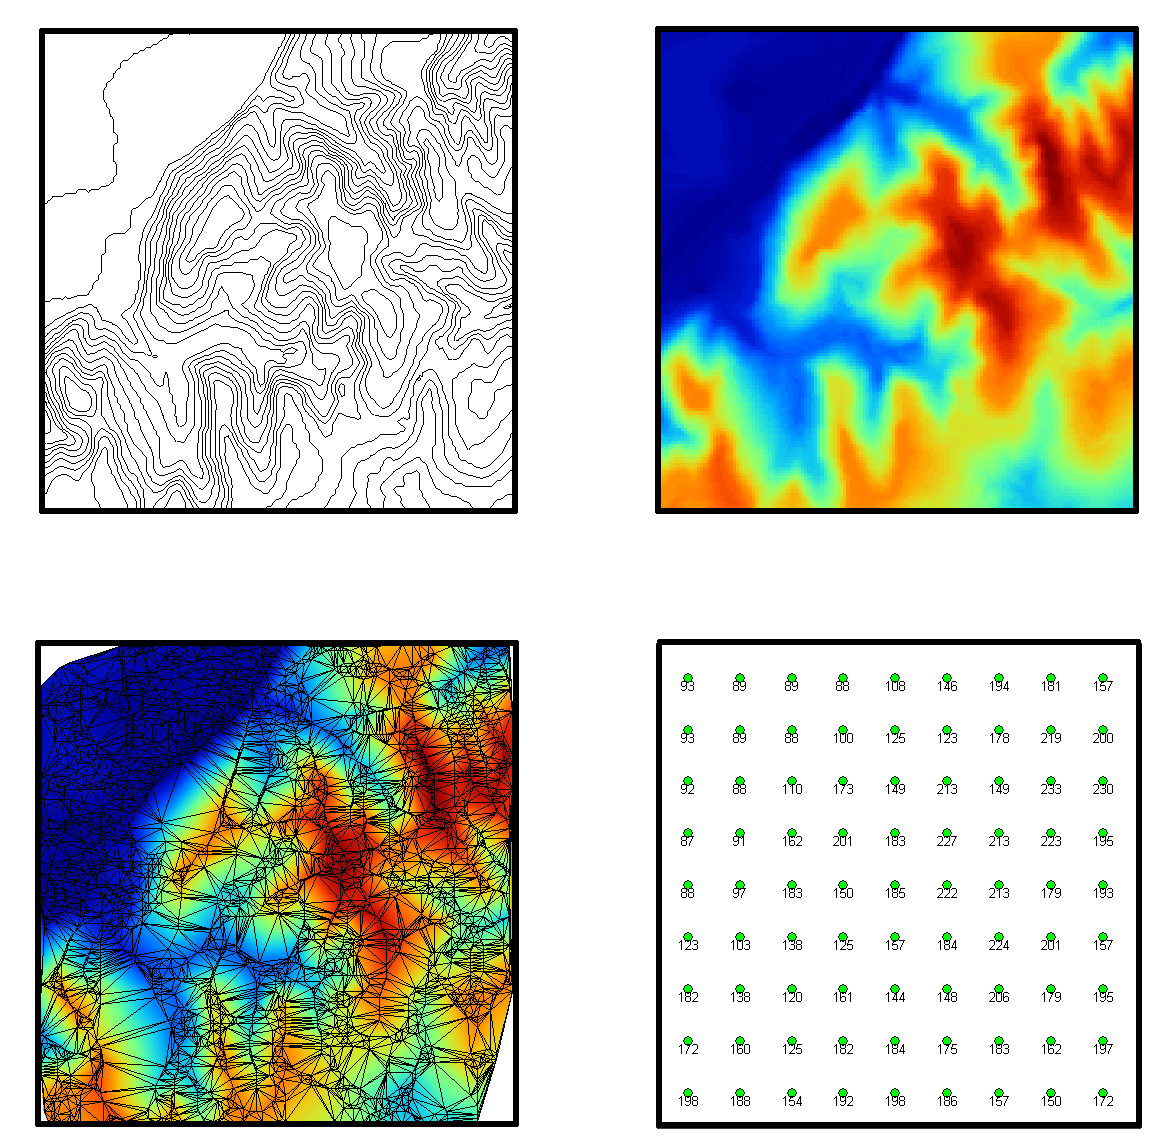
\includegraphics[width=.9\textwidth]{Tipos_datos/MDE_modelos_representacion.png}
\caption{\small Distintas formas de representar una capa con informaci�n altitudinal.}
\label{Fig:MDE_modelos_representacion} 
\end{figure}

\begin{figure}[!hbt]   
\centering
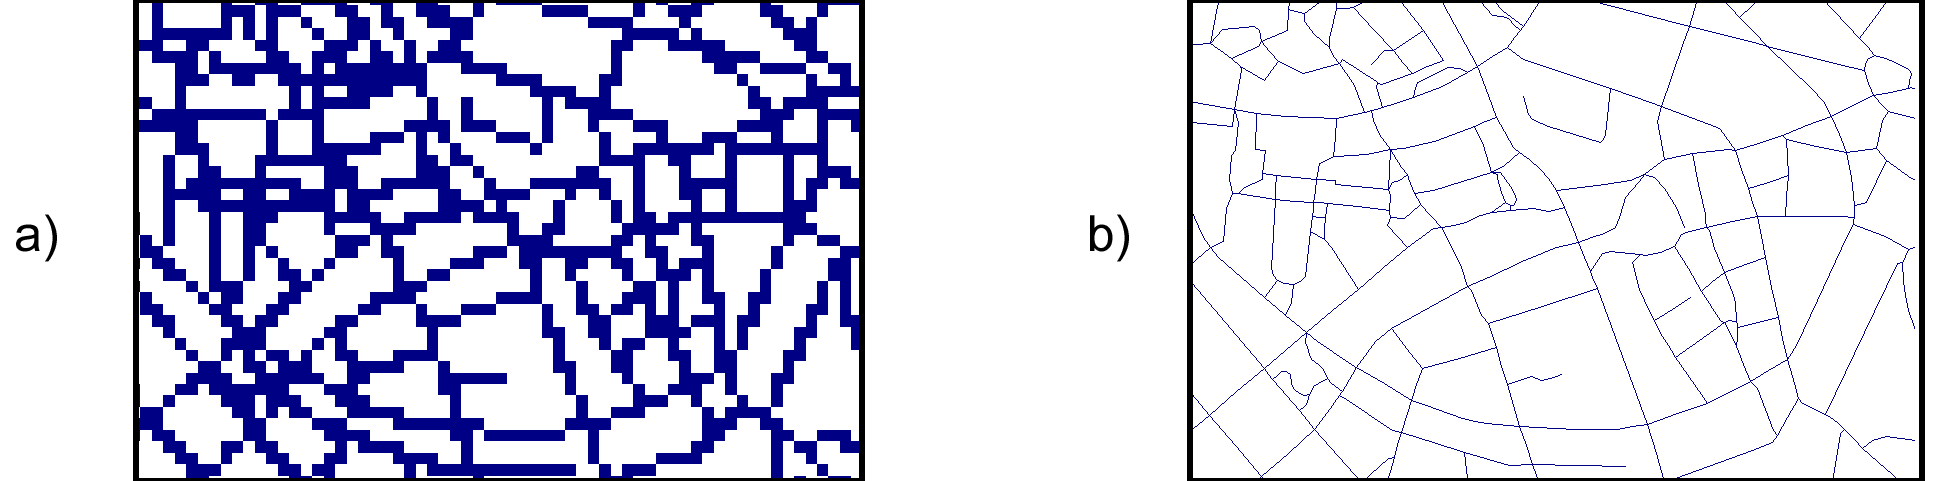
\includegraphics[width=.9\textwidth]{Tipos_datos/Vias_modelos_representacion.png}
\caption{\small Distintas formas de representar una capa con informaci�n sobre una red viaria.}
\label{Fig:Vias_modelos_representacion} 
\end{figure}

Comenzando con la elevaci�n, encontramos cuatro distintas formas de representarla, a saber:

\begin{itemize}
 \item \textbf{Curvas de nivel}. La representaci�n cl�sica empleada tradicionalmente en los mapas de papel. Se recoge la elevaci�n en una serie de curvas, que marcan los puntos en los que dicha elevaci�n es m�ltiplo de una cierta cantidad (la equidistancia). En el ejemplo propuesto, se muestran curvas con elevaciones m�ltiplos de 10 metros.
\item \textbf{Una malla de celdas regulares}, en cada una de las cuales se dispone un valor, que corresponde a las caracter�sticas de la zona ocupada por dicha celda. En este caso, cada celda tiene un valor de altura propio, que al convertirse en un color mediante el uso de una escala de colores, da lugar a la imagen mostrada.
\item \textbf{Puntos regulares}. Una serie de puntos regularmente espaciados. Existe informaci�n de la elevaci�n solo en dichos puntos. La informaci�n se muestra como etiqueta asociada a cada punto.
\item \textbf{Red de Tri�ngulos Irregulares}. Una Red de Tri�ngulos Irregulares (TIN en sus siglas inglesas, de \emph{Triangulated Irregular Network}), es una estructura en la cual se toman los puntos m�s caracter�sticos del relieve y en base a ellos se construye una teselaci�n en tri�ngulos con unas condiciones particulares. Cada uno de los tri�ngulos posee unas propiedades comunes en cuanto a su relieve. Veremos m�s adelante en detalle este tipo de estructuras. Por el momento, basta recordar que los elementos b�sicos de esta forma de representaci�n son tri�ngulos.
\end{itemize}\index{Triangulated Irregular Network (TIN)}

Para el caso de las v�as encontramos dos representaciones distintas:

\begin{itemize}
 \item \textbf{Una malla de celdas} como la citada en el caso anterior. Las celdas de v�a tienen un valor (representado aqu� en azul) distinto de las que se encuentran fuera de la v�a (con valor representado aqu� en blanco)
\item \textbf{Un conjunto de l�neas} representando los trazados de las v�as.
\end{itemize}

En este ultimo caso las celdas se han elegido de un tama�o excesivamente grande, con el fin de que pueda apreciarse de forma inmediata la diferencia existente. Veremos m�s adelante que, como no es dif�cil intuir, la representaci�n mediante celdas no es tan adecuada para el caso de una capa de v�as (aunque para el caso de la elevaci�n da lugar a una imagen con un aspecto inmejorable y altamente informativo), cuando estudiemos los aspectos relativos a la precisi�n en los distintos modelos de almacenamiento. 

Como vemos, para un mismo tipo de informaci�n existen diversas alternativas en cuanto a la forma de materializar la realidad y plasmar el modelo geogr�fico concreto. Estas formas las podemos clasificar en dos grupos principales: modelo de representaci�n \emph{r�ster} y modelo de representaci�n \emph{vectorial}. 

\index{Raster!modelo}\index{Vectorial!modelo}

Si se han seguido los cap�tulos de partes anteriores, probablemente los t�rminos \emph{r�ster} y \emph{vectorial} no resulten extra�os, ya que han aparecido con cierta frecuencia. Esto es as� porque, adem�s de definir dichos t�rminos los principales modelos de representaci�n de la informaci�n geogr�fica dentro de un SIG, se han venido utilizando tradicionalmente para definir a los SIG en s�, en funci�n de si sus capacidades se hallaban m�s enfocadas al manejo y an�lisis de informaci�n en formato r�ster o en formato vectorial. A d�a de hoy, esa diferencia no es tan patente y los SIG m�s habituales pueden trabajar con ambos indistintamente, pudiendo realizar las tareas que resultan m�s adecuadas de llevar a cabo tanto con uno como con otro tipo de representaci�n. 

En lineas generales podemos decir que el modelo r�ster se basa en una divisi�n sistem�tica del espacio, la cual cubre todo este (a este concepto se le denomina se denomina \emph{teselaci�n}), caracteriz�ndolo como un conjunto de unidades elementales (las celdas de las mallas vistas en los ejemplos). El modelo vectorial, por su parte, no divide el espacio completamente, sino que lo define mediante una serie de elementos geom�tricos con valores asociados, siendo la disposici�n de estos no sistem�tica, sino guardando relaci�n con los objetos geogr�ficos presentes en la zona de estudio.

\index{Teselaci�n}

En un principio, puede pensarse que el modelo r�ster se asemeja al modelo geogr�fico de campos, mientras que el vectorial concuerda con el de entidades discretas. Aunque en cierta medida puede considerarse que as� sucede y existe tal dualidad, no es del todo cierta esta equiparaci�n, como discutiremos con algo m�s de detalle en los siguientes puntos.

De forma esquem�tica, los enfoques de los modelos de representaci�n r�ster y vectorial se muestran en la figura \ref{Fig:Esquemas_modelos_representacion}

\begin{figure}[!hbt]   
\centering
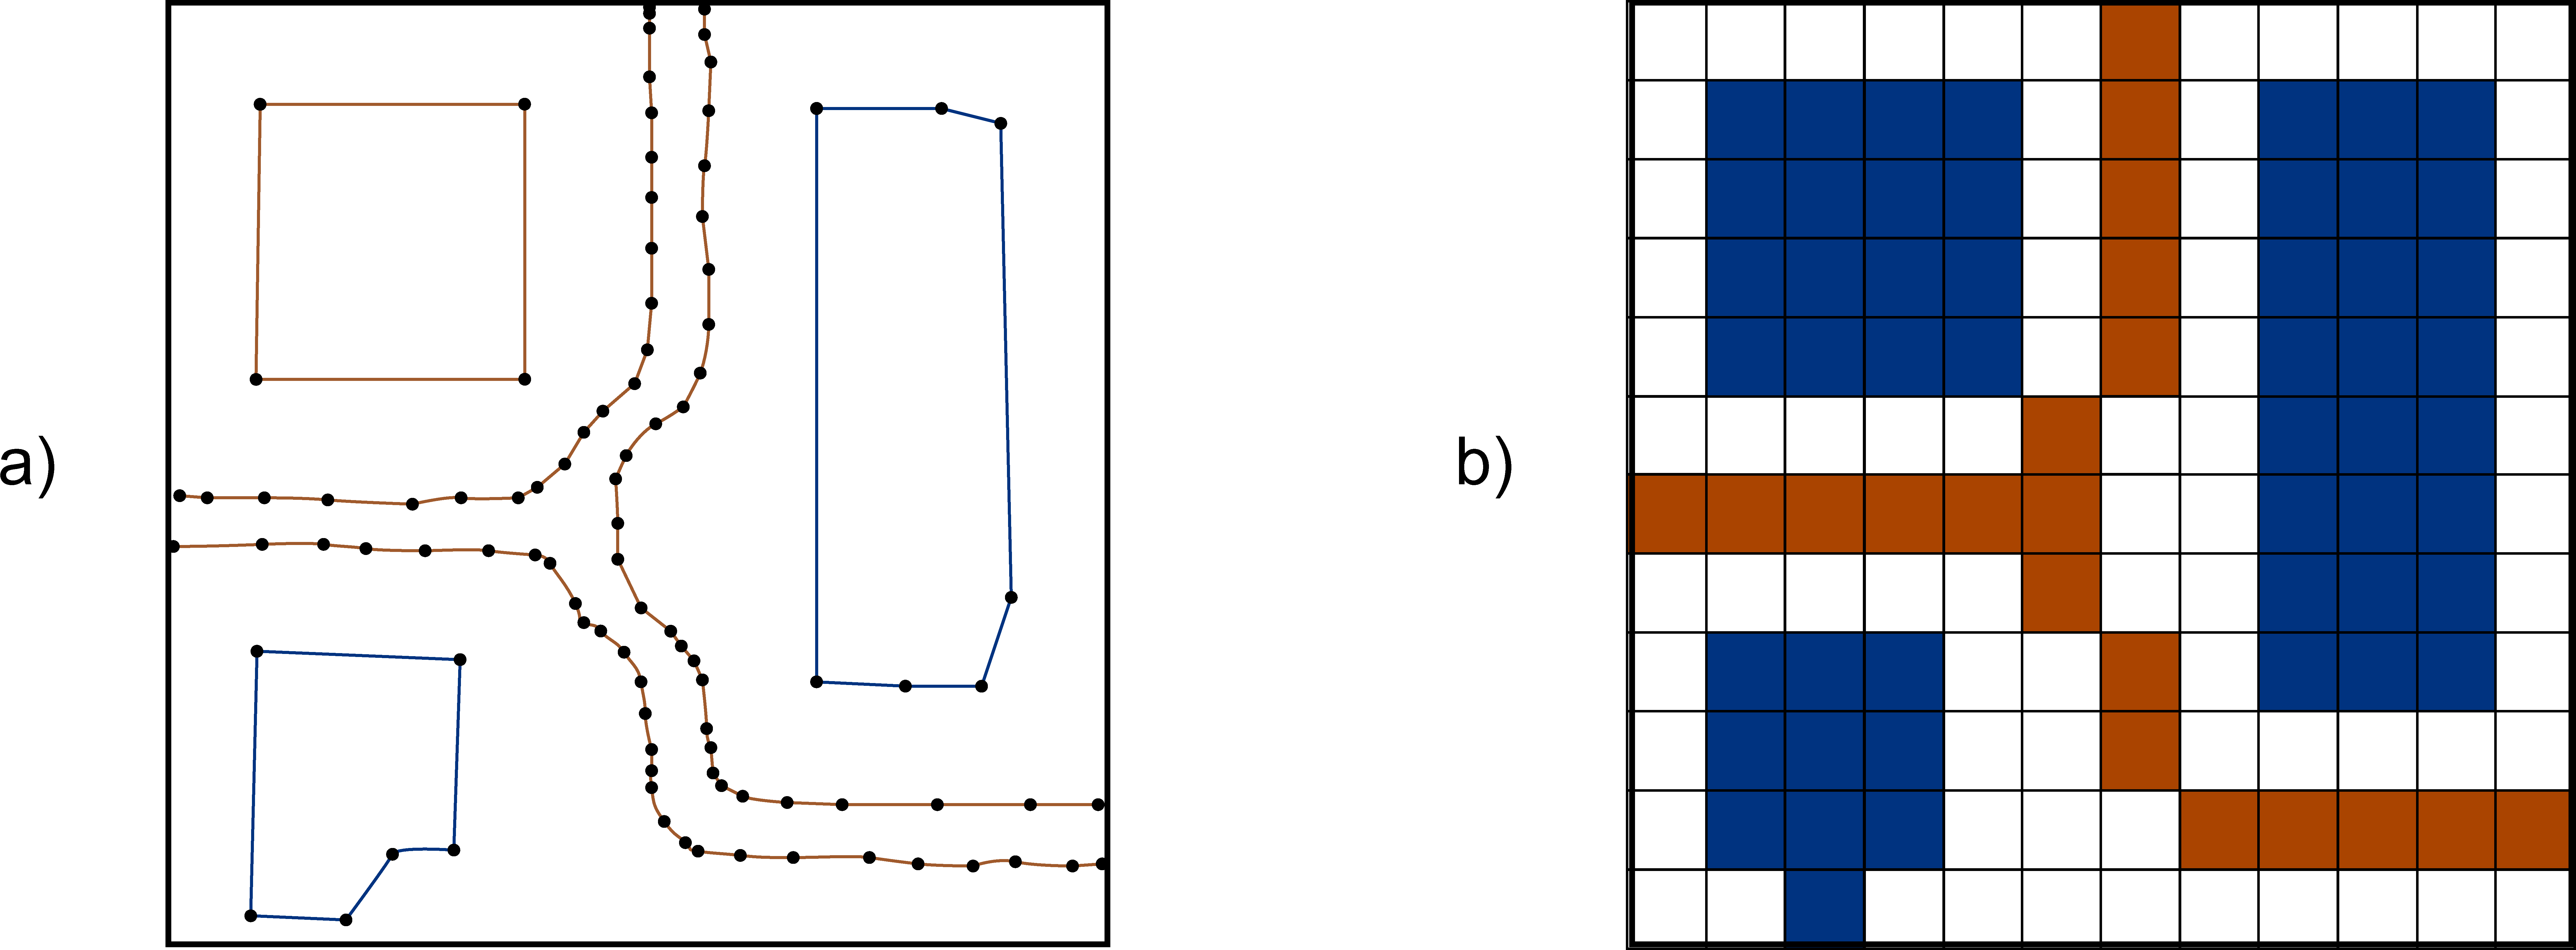
\includegraphics[width=.9\textwidth]{Tipos_datos/Esquemas_modelos_representacion.pdf}
\caption{\small Comparaci�n entre los esquemas del modelo de representaci�n vectorial (a) y r�ster (b).}
\label{Fig:Esquemas_modelos_representacion} 
\end{figure}

Podemos entender estos enfoques haciendo uso del esquema de Sinton presentado con anterioridad. En el modelo vectorial controlamos la definici�n de los valores asociados, y medimos la localizaci�n y forma de estos, dejando fijo el tiempo. En el modelo r�ster, aunque la componente temporal tambi�n es fija, la componente que controlamos es la espacial (a trav�s de la sistematicidad de la malla), mientras que medimos la naturaleza de los valores en cada una de las celdas.

\index{Sinton!esquema de}

Antes de pasar a la definici�n detallada de los modelos r�ster y vectorial, mencionar que, como modelos principales empleados para la definici�n de capas de informaci�n geogr�fica, las expresiones \emph{capa vectorial} y \emph{capa r�ster} son de uso habitual, y se emplear�n de aqu� en adelante tanto en este como en posteriores cap�tulos.

\subsection{Modelo r�ster}
\label{Modelo_raster}\index{Raster!modelo}

En el modelo r�ster, la zona de estudio se divide de forma sistem�tica en una serie de unidades m�nimas (denominadas habitualmente \emph{celdas}), y para cada una de estas se recoge la informaci�n pertinente que la describe.  Se puede ver esto en detalle en la figura \ref{Fig:Raster_closeup}, que muestra aumentada una porci�n la malla r�ster de elevaciones de la figura \ref{Fig:MDE_modelos_representacion}, de modo que los l�mites de las celdas se hacen patentes y puede adem�s representarse en cada una de ellas su valor asociado.

\begin{figure}[!hbt]   
\centering
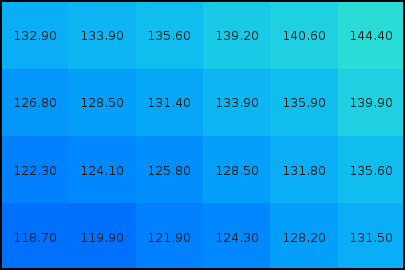
\includegraphics[width=.4\textwidth]{Tipos_datos/Raster_closeup.png}
\caption{\small Celdas de una malla r�ster con sus valores asociados.}
\label{Fig:Raster_closeup} 
\end{figure}

Aunque la malla de celdas puede contener informaci�n sobre varias variables, lo habitual es que trate una �nica variable. Es decir, que se tenga un �nico valor para cada una de las celdas.

La caracter�stica principal del modelo r�ster, y que le confiere gran parte de sus propiedades m�s interesantes, especialmente de cara al an�lisis, es su sistematicidad. La divisi�n del espacio en unidades m�nimas se lleva a cabo de forma sistem�tica de acuerdo con alg�n patr�n, de tal modo que existe una relaci�n impl�cita entre las celdas, ya que estas son contiguas entre s�, cubren todo el espacio, y no se solapan. Por tanto, la posici�n de una celda depende de la de las restantes, para as� conformar en conjunto toda la malla regular que cumple las anteriores caracter�sticas. Dicho de otro modo, el orden propio de las celdas, presente gracias a la divisi�n sistem�tica realizada, aporta un elemento adicional que las relaciona entre s�.

\index{Raster! de celdas no rectangulares}

Como unidad m�nima pueden tomarse elementos de diversas formas. La m�s habitual es mediante unidades de forma cuadrada, aunque tambi�n pueden ser formas rectangulares, o incluso triangulares o hexagonales \cite{Diaz1986Reading}. No obstante, los SIG habituales se limitan a modelos de celdas cuadradas, y las implementaciones de otros modelos son de uso muy reducido y en aplicaciones muy especificas que en general no est�n orientadas al uso general ni disponibles de forma accesible al usuario com�n. Junto a esto, la informaci�n geogr�fica en formatos r�ster distintos de la divisi�n en celdas cuadradas es pr�cticamente inexistente, haciendo m�s dif�cil el empleo de estos formatos en condiciones normales de trabajo.

De igual modo, existen representaciones r�ster no regulares, en las que todas las unidades m�nimas no tienen un mismo tama�o. Este tipo de representaciones no tiene apenas presencia en los SIG, pero son habituales en otros �mbitos tales como el de las representaciones 3D, con unos requerimientos bien distintos\footnote{V�ase, por ejemplo, el concepto de Nivel Continuo de Detalle (Continuous Level of Detail, CLOD), para lograr representaciones de detalle con el menor gasto de recursos posible, y que es habitual en este campo.}. Esto est� relacionado a su vez con los modelos de almacenamiento r�ster, que veremos m�s adelante en este mismo cap�tulo.

\index{Continuous Level of Detail (CLOD)}

En todos los casos, la divisi�n en celdas no depende de la variable estudiada, y es una divisi�n geogr�fica. Esto lo diferencia de otras divisiones como el caso de la Red de Tri�ngulos Irregulares, que, a pesar de ser una teselacion que cubre todo el espacio, est� basada en la propia variable de elevaci�n, y dicha divisi�n (n�mero, forma y disposici�n de los tri�ngulos) ser�a distinta en caso de que los valores de elevaci�n fueran otros.

\index{Triangulated Irregular Network (TIN)}

Siendo, pues, las mallas r�ster de celdas cuadradas las m�s habituales, pasemos a ver algo m�s acerca de estas y su elementos b�sicos. Dos son los elementos principales que resultan necesarios para una definici�n completa de una capa r�ster:

\begin{itemize}
\item Una localizaci�n geogr�fica exacta de alguna celda y una distancia entre celdas, para en base a ellas, y en virtud de la regularidad de la malla, conocer las coordenadas de las restantes.
\item Un conjunto de valores correspondientes a las celdas.
\end{itemize}

En el modelo r�ster no se recogen de forma expl�cita las coordenadas de cada una de las celdas, sino tan solo los valores de estas. No resulta necesario acompa�ar a dichos valores de un emplazamiento espacial concreto, pues hacen referencia a un elemento particular de la malla, la cual representa una estructura fija y regular. No obstante, s� que es necesario emplazar dicha malla en el espacio para despu�s poder calcular las coordenadas particulares de cada celda.

Lo m�s habitual es definir el emplazamiento de una �nica celda (habitualmente la celda superior izquierda), una orientaci�n fija, y una distancia entre las celdas (el paso de la malla). Como se muestra en la figura \ref{Fig:Elementos_capa_raster}, esto ya permite, mediante un sencillo c�lculo, conocer las coordenadas de todas las celdas sin necesidad de almacenar estas.

\begin{figure}[!hbt]   
\centering
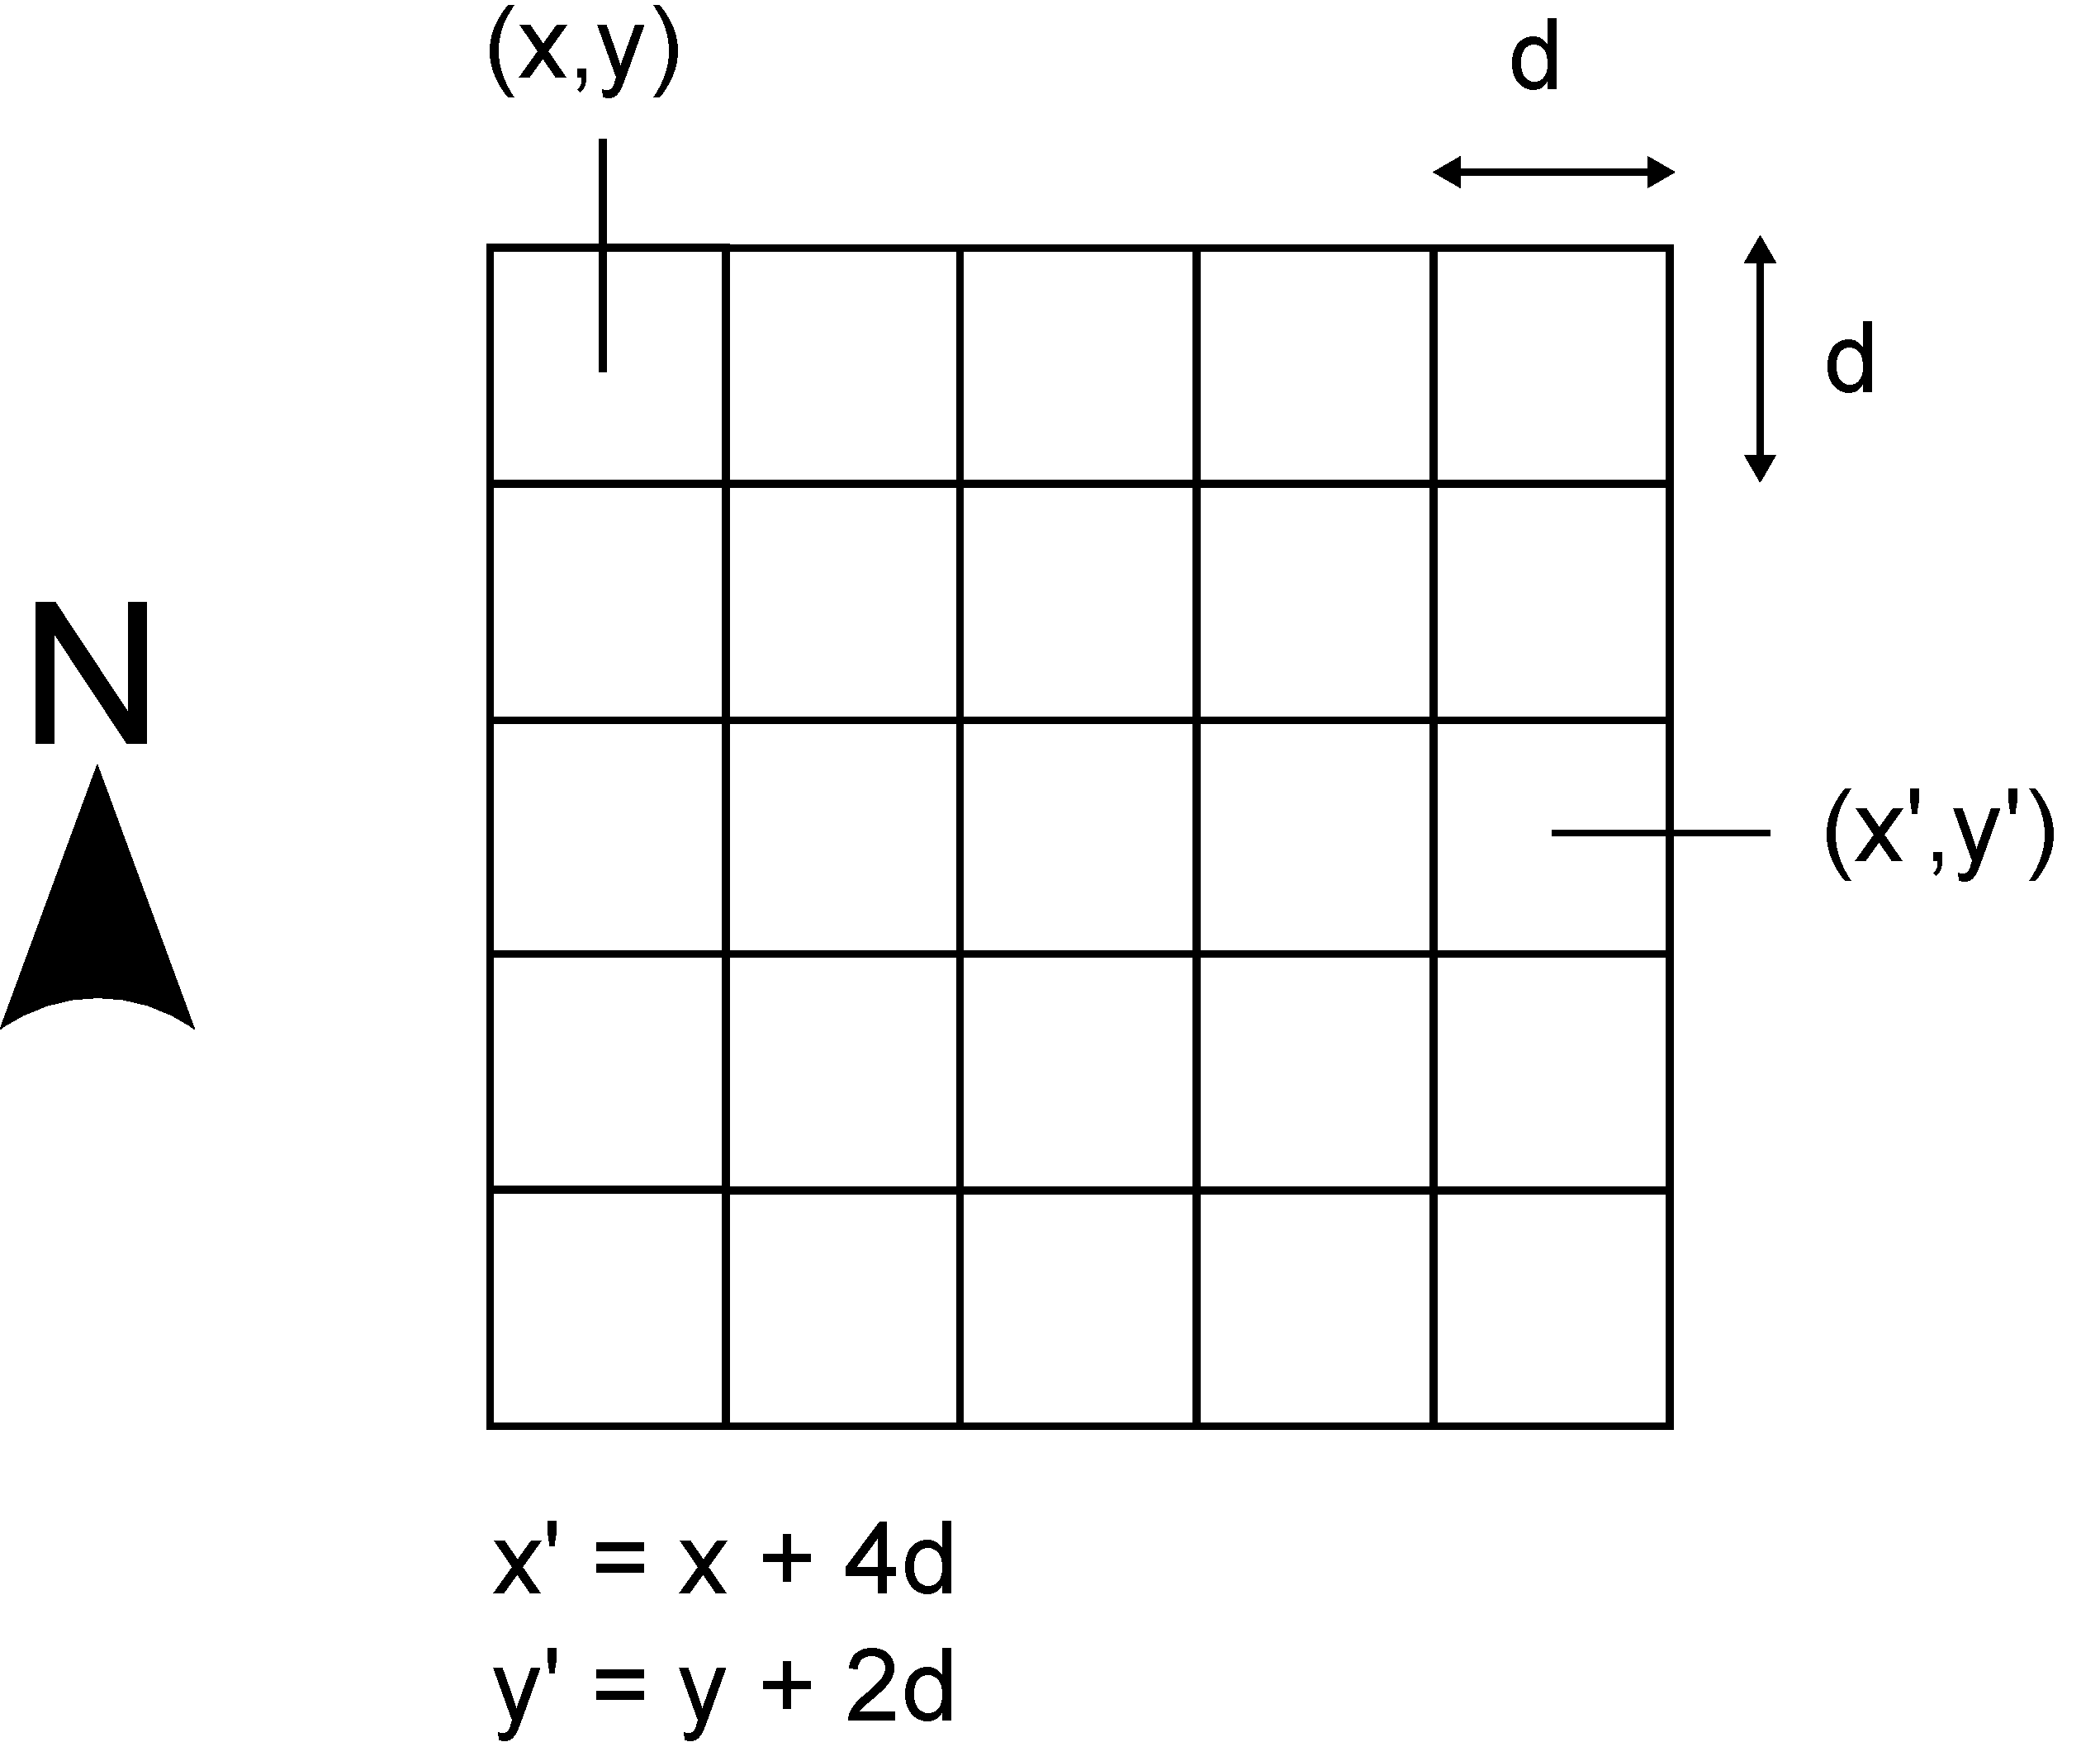
\includegraphics[width=.4\textwidth]{Tipos_datos/Elementos_capa_raster.pdf}
\caption{\small La estructura regular de la malla r�ster permite conocer las coordenadas de las celdas sin necesidad de almacenar estas, sino tan solo recogiendo algunos par�metros de la malla como la localizaci�n de una celda base ($x,y$), la orientaci�n global o el tama�o de celda ($d$).}
\label{Fig:Elementos_capa_raster} 
\end{figure}

La orientaci�n de las capas r�ster es habitualmente Norte--Sur, de tal modo que si pasamos de la primera a la segunda fila estamos descendiendo en latitud (este hecho ser�a matizable en funci�n de la proyecci�n empleada). Dicho de otra forma, la parte de arriba de la imagen es el norte, y la de abajo es el sur. Esta convenci�n simplifica el trabajo con capas r�ster dentro de un SIG y permite aplicar directamente la f�rmula mostrada en la figura \ref{Fig:Elementos_capa_raster}.

No obstante, puede suceder que la fuente de datos original no se adhiera a este formato (por ejemplo, una fotograf�a a�rea en la que el avi�n no volaba en direcci�n Norte--Sur o perpendicular, o una porci�n de un mapa escaneado que no tiene tampoco esa orientaci�n). En tal caso, y puesto que los SIG trabajan en general con tal orientaci�n en sus representaciones y a la hora de incorporar capas r�ster, nos encontraremos con situaciones como la mostrada en la figura \ref{Fig:Malla_raster_rotada}

\begin{figure}[!hbt]   
\centering
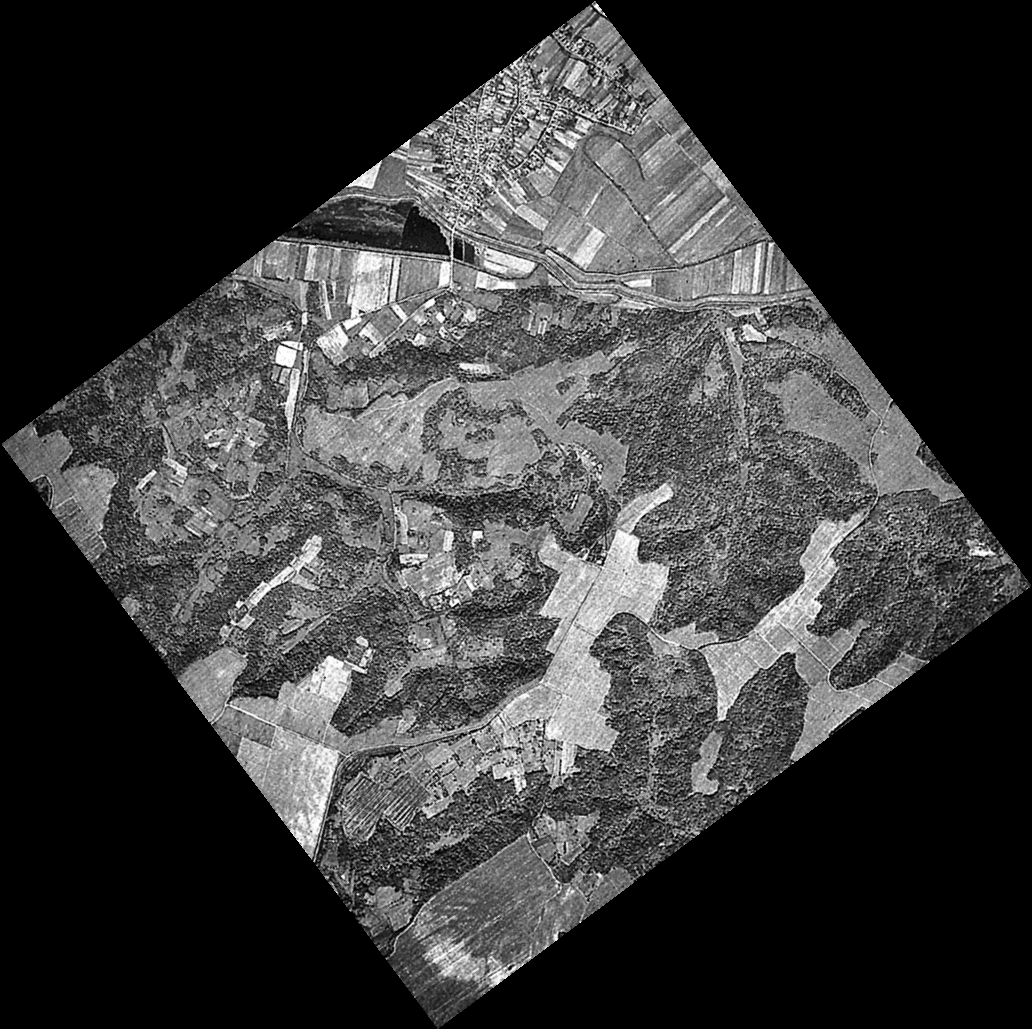
\includegraphics[width=.5\textwidth]{Tipos_datos/Malla_raster_rotada.png}
\caption{\small Aunque la zona de estudio no tenga orientaci�n Norte--Sur, los SIG trabajan habitualmente con esta orientaci�n, y las im�genes deben adecuarse a ello.}
\label{Fig:Malla_raster_rotada} 
\end{figure}

En ella vemos c�mo la orientaci�n de la banda de estudio recogida es distinta de la Norte--Sur  de la imagen, lo cual, unido a la forma rectangular que ha de tener dicha imagen, causa la aparici�n de zonas sin informaci�n (en negro). Esto implica por una parte la necesidad de almacenar un gran n�mero de valores sin inter�s, y por otra la necesidad de especificar de alg�n modo que todas esas celdas que aparecen en negro en la imagen son realmente celdas para las cuales no se dispone de informaci�n. Esto �ltimo se suele llevar a cabo mediante la definici�n de un valor arbitrario que indique la falta de datos (denominado generalmente valor de \emph{sin datos}), que codifica tal situaci�n, de tal modo que pueden ignorarse las celdas con dicho valor a la hora de representar o analizar la capa r�ster en cuesti�n. \index{Sin datos!valor de}

El otro par�metro necesario junto con la orientaci�n de la malla y la situaci�n geogr�fica de una de sus celdas es el denominado \emph{tama�o de celda} o \emph{tama�o de p�xel}, tambi�n conocido como \emph{resoluci�n}, pues, en efecto, su magnitud define la resoluci�n de la capa. Un tama�o de celda mayor implica una menor resoluci�n, y viceversa.\index{Resoluci�n}\index{Tama�o!de celda}\index{Tama�o!de p�xel}

Adem�s de servir para el c�lculo de coordenadas de las celdas y definir la estructura de la malla, el tama�o de celda permite calcular �reas, ya que establece el �rea ocupada por cada celda. Asimismo, y como aspecto m�s relevante, el tama�o de celda determina la precisi�n con la que se recoge una variable dentro de una capa r�ster, y puede considerarse como el equivalente conceptual a la escala de dicha capa. Por esta raz�n, es importante trabajar con capas r�ster de un tama�o de celda adecuado para el tipo de an�lisis o tarea que quiera desarrollarse.

As�, un an�lisis microtopogr�fico en el cual resulta necesario registrar la variaci�n del relieve a peque�a escala no puede llevarse a cabo con una capa de elevaciones con tama�o de celda de 100 metros, ya que toda la variabilidad menor a esos 100 metros se pierde. No debe olvidarse que cada celda registra un �nico valor de la variable, y esta se considera constante dentro de dicha celda. Un tama�o de 100 metros implicar�a la recogida de un �nico valor para cada hect�rea de terreno, lo cual no es suficiente en este caso.

Muchos son los factores que influyen en el tama�o de celda de una capa r�ster, entre ellos las caracter�sticas de los datos iniciales con los que se ha creado dicha capa o los medios particulares con que estos han sido recogidos. En la figura \ref{Fig:Diferentes_resoluciones} pueden observarse dos im�genes a�reas del juego de datos de ejemplo (las im�genes son un tipo particular de capa r�ster, como en breve veremos), con distinta resoluci�n. Esta, al ser distinta, las hace v�lidas para uno u otro tipo de uso. Vemos claramente que en en la imagen en blanco y negro (cuyo tama�o de p�xel es de 5 metros) se distinguen las distintas �reas de cultivo, mientras que en la imagen en color (con tama�o de p�xel de 25 metros), estos no se distinguen. Todos aquellos an�lisis que requieran disponer de informaci�n por debajo de esos 25 metros, no podr�n ser llevados a cabo con esta �ltima imagen.

Para el caso de capas r�ster de variables continuas, en la secci�n \ref{Eleccion_caracteristicas_capa_resultante_raster} se da informaci�n detallada sobre c�mo definir el tama�o de celda �ptimo a la hora de crear estas a partir de datos de otra clase tales como datos vectoriales.

\begin{figure}[!hbt]   
\centering
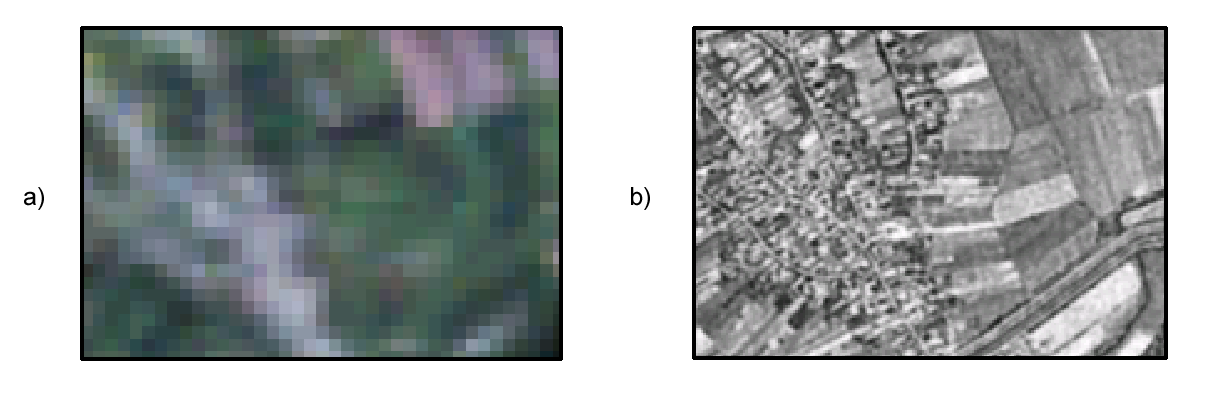
\includegraphics[width=\textwidth]{Tipos_datos/Diferentes_resoluciones.png}
\caption{\small Im�genes de diferente resoluci�n en funci�n del sensor con que han sido obtenidas. Al tener distintos tama�os de p�xel, servir�n para distintos usos dentro de un SIG.}
\label{Fig:Diferentes_resoluciones} 
\end{figure}

Una vez conocemos el formato r�ster, podemos relacionarlo con lo que ya hemos visto relativo a los modelos geogr�ficos. En primer lugar, y por sus propias caracter�sticas, puede pensarse que la representaci�n r�ster es m�s adecuada para variables de tipo continuo que var�an a su vez de forma continua en el espacio geogr�fico. Es decir, es m�s pr�xima al modelo geogr�fico de campos que al de entidades discretas. Esto es as� debido principalmente a que una capa r�ster cubre todo el espacio, y ello favorece el estudio de dicha variabilidad. No obstante, no debe considerarse que el �mbito de las variables continuas y los campos es exclusivo de las capas r�ster. De hecho, de las cuatro representaciones mostradas para el caso de la elevaci�n, solo una de ellas es de tipo r�ster.

S� es cierto, no obstante, que el formato r�ster es especialmente adecuado para el an�lisis de la informaci�n geogr�fica, en especial cuando esta es de tipo continuo. Esto es as� porque el principal elemento de las capas r�ster es, como ya se ha dicho, su estructura sistem�tica. Si a esta le unimos la regularidad que se presenta en la forma m�s extendida de representaci�n r�ster (la de celdas cuadradas regulares), tenemos un modelo �ptimo para el an�lisis, que simplifica en gran medida este y hace m�s sencilla la implementaci�n de los algoritmos correspondientes. Es por ello que, tradicionalmente, los SIG con mayor soporte para datos r�ster han sido aquellos que presentaban a su vez un mayor n�mero de funcionalidades de an�lisis en �reas tales como el estudio del relieve, el an�lisis de costes u otros similares.

No obstante, ello no restringe el alcance del formato. Variables que no resulta tan �ptimo concebir como campos, tales como una red vial, tambi�n puede expresarse como una capa r�ster, como hemos visto en la figura \ref{Fig:Vias_modelos_representacion}.

\subsubsection{El caso de las im�genes}

Un caso especial de capa r�ster son las im�genes, de las que hemos visto ya un ejemplo al tratar el tama�o de celda. Tanto si estas proceden de un sensor digital o bien han sido escaneadas, los sensores correspondientes generan una estructura en forma de malla que se ajusta al modelo de representaci�n r�ster. Este hecho tiene gran importancia, pues facilita el an�lisis conjunto de im�genes y capas de datos con otro tipo de informaci�n, haciendo que este sea sumamente m�s sencillo, al compartir el modelo de representaci�n.

Mientras que, como hemos visto en los ejemplos, una misma informaci�n se puede recoger en formatos r�ster y vectorial, las im�genes se recogen �nicamente en formato r�ster, tanto por ser ese modelo mucho m�s adecuado, como por ser mucho m�s coherente con el tipo de informaci�n y la procedencia de esta.

El concepto de celda en una malla r�ster es el equivalente al de p�xel\footnote{acr�nimo de \emph{picture element}}, bien conocido en el campo de las im�genes digitales. As�, cuando decimos que una c�mara digital tiene tres megap�xeles, queremos decir que captura un total de tres millones de p�xeles. De otra forma, la malla r�ster que se genera tiene tres millones de celdas. Las im�genes con las que trabajamos en un SIG no se diferencian de las que tomamos con una c�mara digital, salvo en el hecho particular de que representan una porci�n de terreno dentro de un sistema de coordenadas dado, pero la estructura es la misma: una malla de celdas (p�xeles).\index{Pixel}

Otra particularidad de las im�genes es la presencia de \emph{bandas}\index{Bandas}. Los valores recogidos en las im�genes indican de forma general la reflectancia\index{Reflectancia} en una determinada longitud de onda (esto se explica con mayor detalle en los cap�tulos \ref{Fuentes_datos} y \ref{Procesado_imagenes}). Puesto que el espectro de radiaci�n\index{Espectro electromagn�tico} puede subdividirse en distintos grupos, los sensores que toman estas im�genes recogen varias capas, una para cada uno de estos grupos. En lugar de almacenarse como un conjunto de capas separadas, es m�s frecuente que lo hagan en una �nica que contiene varias \emph{bandas}, es decir, varios niveles distintos, cada uno de los cuales podr�a constituir por s� mismo una capa r�ster.

Se trata de una diferencia m�s de tipo formal, pero de cierta importancia, puesto que no todos los SIG est�n preparados para manejar capas r�ster con independencia de su n�mero de capas. Im�genes con una �nica banda, o tres, son habituales y soportadas en la mayor�a de implementaciones, mientras que n�meros mayores de bandas no se encuentran soportados en muchos programas.

Todos estos conceptos se extender�n en el cap�tulo \ref{Fuentes_datos}.

\subsection{Modelo vectorial}

El otro modelo principal de representaci�n es el modelo vectorial. En este modelo, no existen unidades fundamentales que dividen la zona recogida, sino que se recoge la variabilidad y caracter�sticas de esta mediante entidades geom�tricas, para cada una de las cuales dichas caracter�sticas son constantes. La forma de estas entidades (su frontera), se codifica de modo explicito, a diferencia del modelo r�ster, donde ven�a impl�cita en la propia estructura de la malla.

Si el modelo r�ster era similar al modelo conceptual de campos, el vectorial lo es al de entidades discretas, pues modeliza el espacio geogr�fico mediante una serie de primitivas geom�tricas que contienen los elementos m�s destacados de dicho espacio. Estas primitivas son de tres tipos: puntos, l�neas y pol�gonos.\index{Primitivas geom�tricas}

\begin{figure}[!hbt]   
\centering
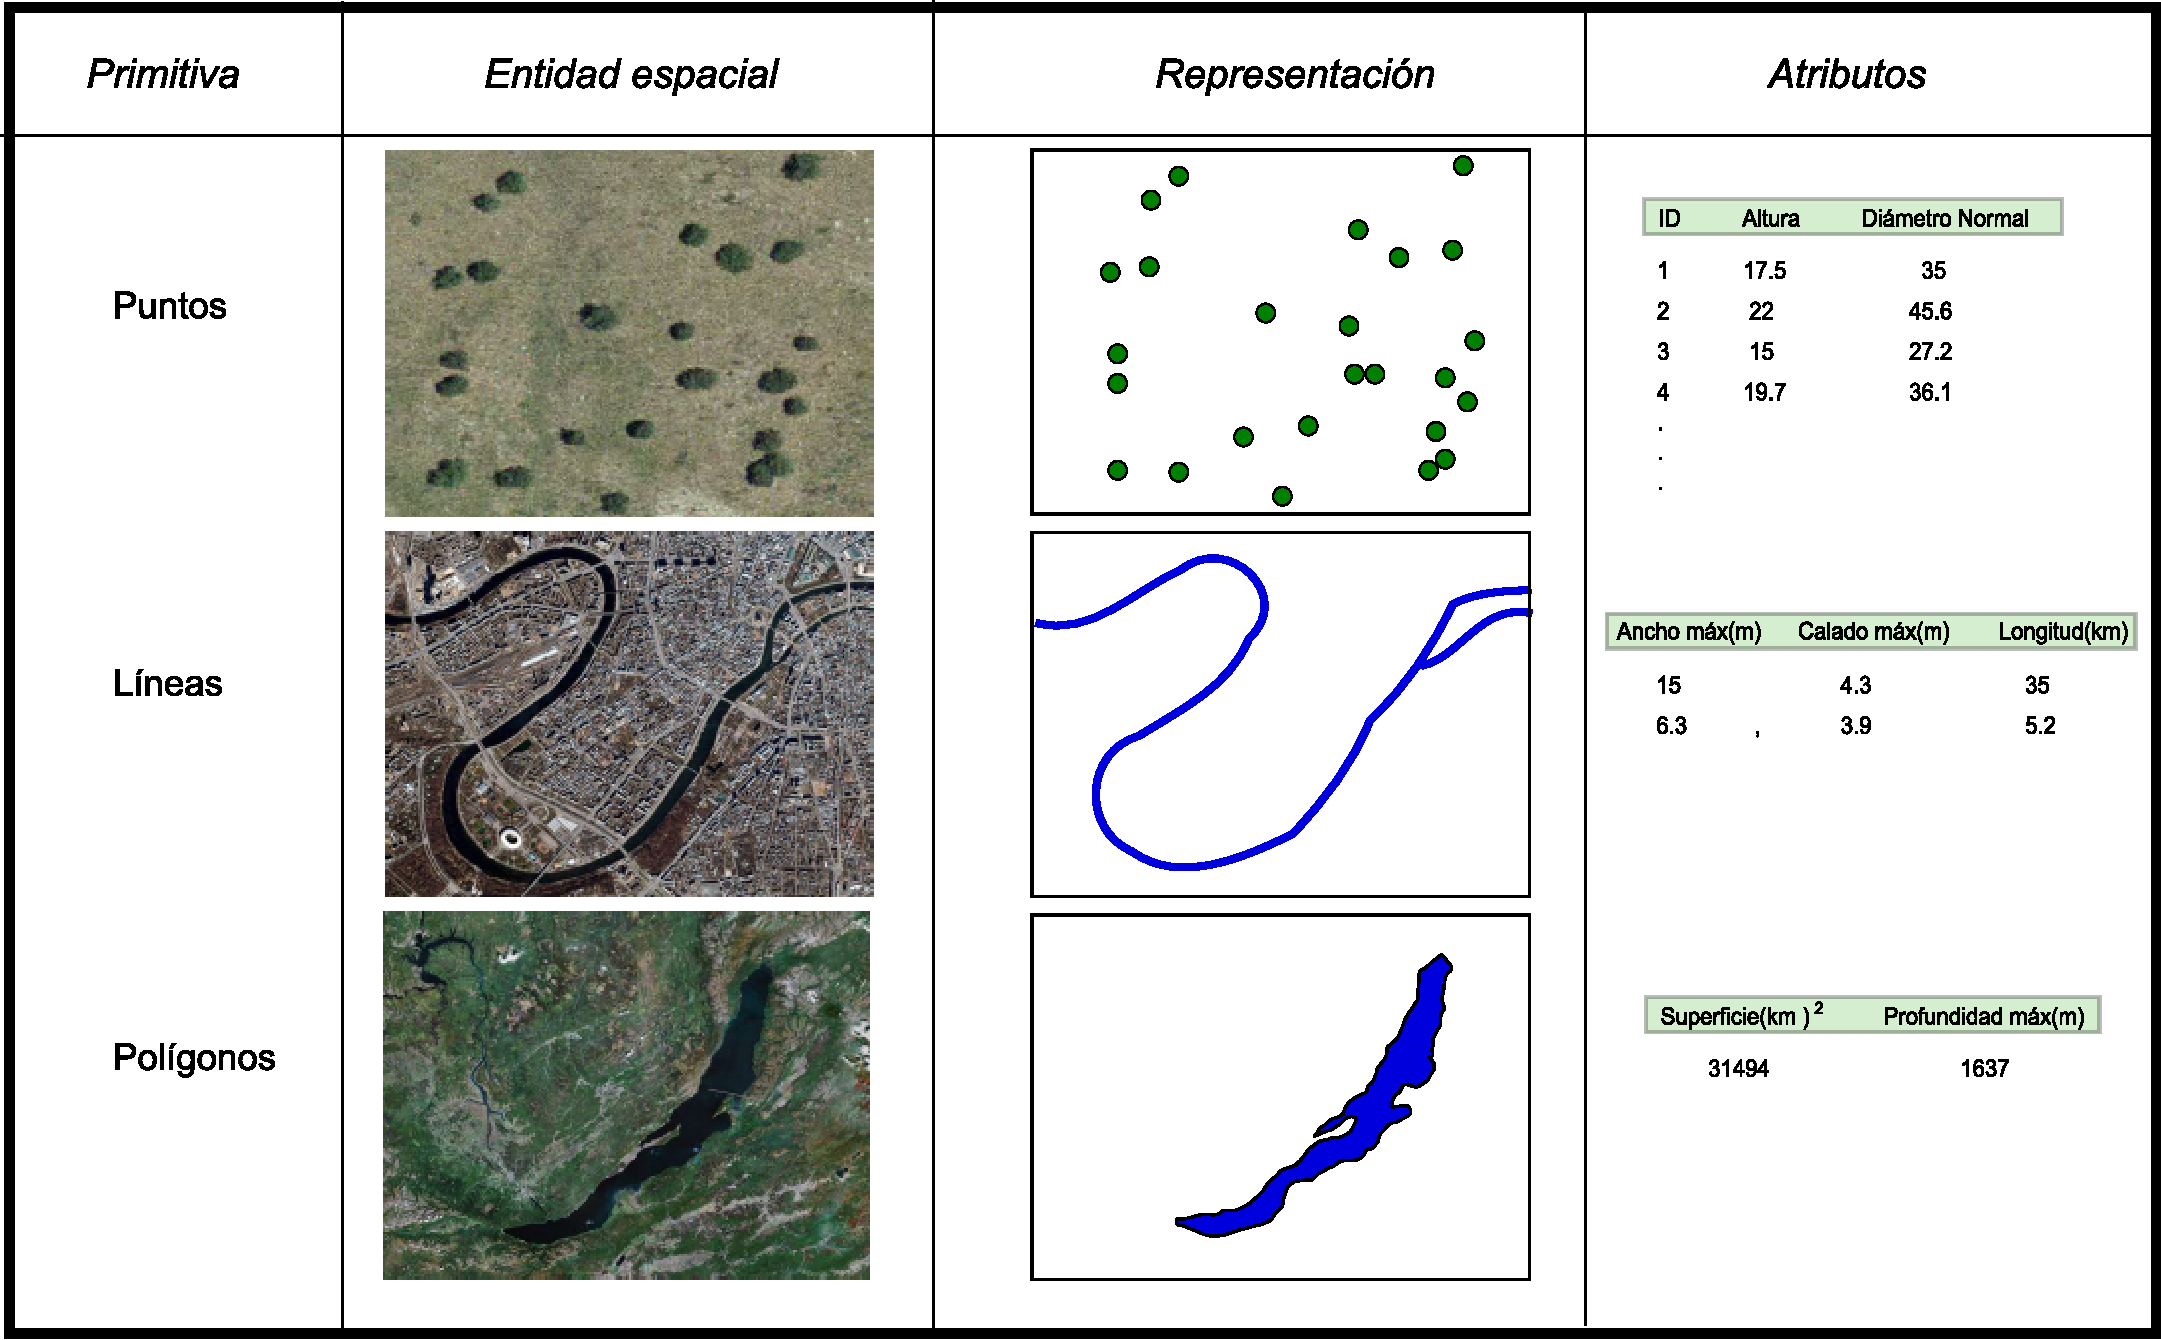
\includegraphics[width=.95\textwidth]{Tipos_datos/Primitivas_vectoriales.pdf}
\caption{\small Primitivas geom�tricas en el modelo de representaci�n vectorial y ejemplos particulares de cada una de ellas con atributos asociados}
\label{Fig:Primitivas_vectoriales} 
\end{figure}

Utilizando puntos, l�neas o pol�gonos, puede modelizarse el espacio geogr�fico si se asocia a estas geometr�as una serie de valores definitorios. La componente espacial de la informaci�n queda as� en la propia primitiva (recoge la forma, posici�n y otras propiedades espaciales), y la componente tem�tica queda en dichos valores asociados (Figura \ref{Fig:Primitivas_vectoriales}).

A la hora de definir las formas geom�tricas b�sicas, todas ellas pueden reducirse en �ltima instancia a puntos. As�, las lineas son un conjunto de puntos interconectados en un determinado orden, y los pol�gonos son l�neas cerradas, tambi�n expresables por tanto como una serie de puntos. Todo elemento del espacio geogr�fico queda definido, pues, por una serie de puntos que determinan sus propiedades espaciales y una serie de valores asociados.

Una �nica entidad (para la cual existir� un �nico conjunto de valores asociados) puede contener varias primitivas. As�, en un mapa mundial en que cada entidad represente un pa�s, y tal y como se ve en la figura \ref{Fig:Casos_particulares_poligonos}, pa�ses como Canad� estar�n representados por m�s de un pol�gono, pues no puede recogerse todo su territorio mediante uno �nico. Todos estos pol�gonos constituyen una �nica entidad, ya que todos perteneces al mismo pa�s y tendr�n el mismo conjunto de valores asociados.

\begin{figure}[!hbt]   
\centering
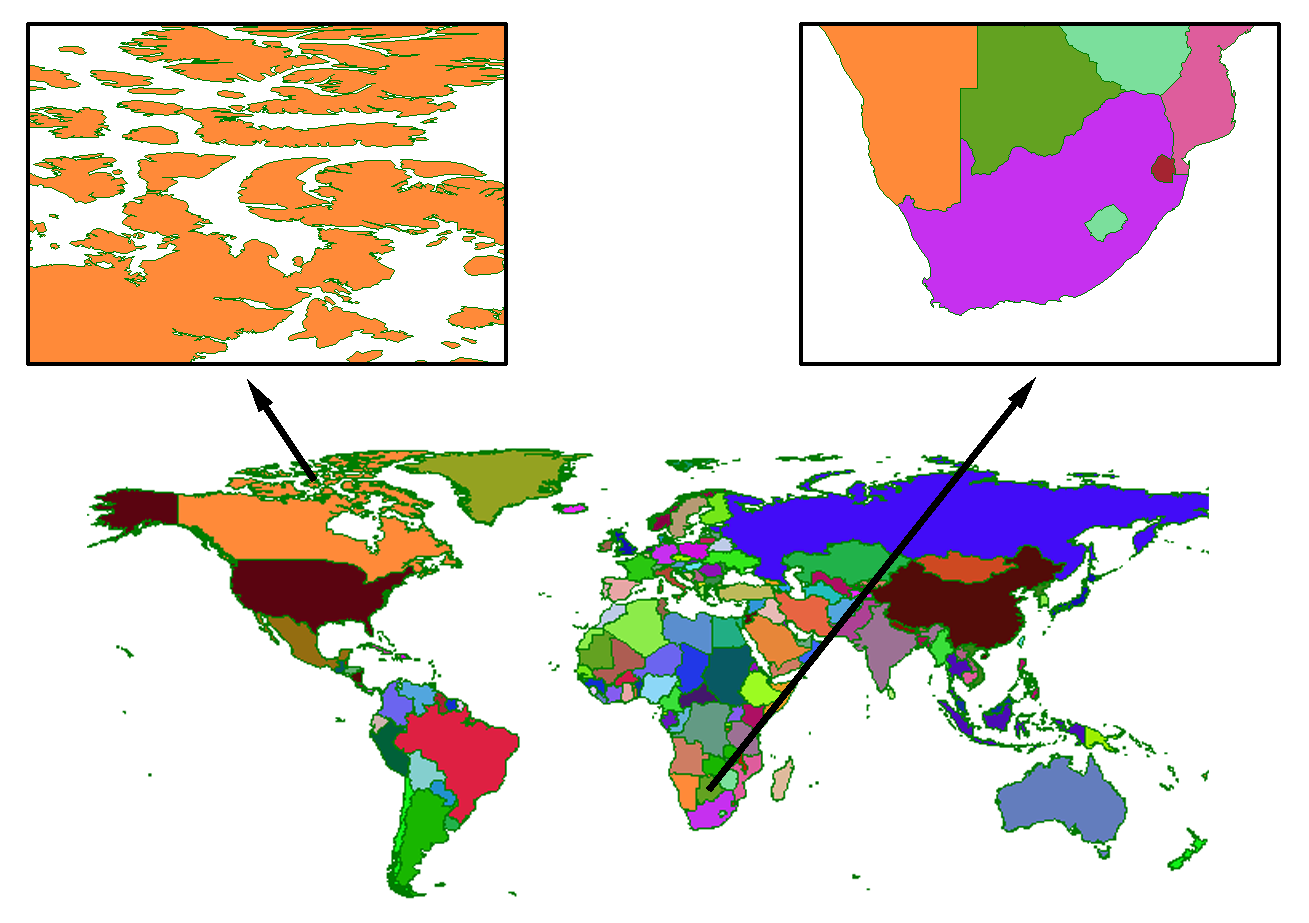
\includegraphics[width=.85\textwidth]{Tipos_datos/Casos_particulares_poligonos.png}
\caption{\small Casos particulares de pol�gonos: a) varios pol�gonos disjuntos en una misma entidad (en este caso, mismo pa�s), b) Pol�gonos con islas (huecos).}
\label{Fig:Casos_particulares_poligonos} 
\end{figure}

\index{Pol�gono!con huecos}\index{Entidades!multiples}

Otro caso particular en las capas de pol�gonos son aquellos pol�gonos con islas (huecos). En este caso, se registran de la misma forma que en el caso de varios pol�gonos disjuntos. Se recogen los propios huecos como pol�gonos independientes, pero recogiendo de alg�n modo tambi�n la circunstancia de que estos pol�gonos no se \emph{suman} a los pol�gonos existentes en esa entidad, sino que se \emph{restan}. As� es, por ejemplo, para el caso del �rea total de pol�gonos de una �nica entidad, ya que el �rea del hueco debe ser restada de la total.

En la figura anterior, vemos como Sud�frica presenta esta situaci�n, ya que dentro del territorio del pa�s hay zonas aislada que no pertenece a Sud�frica, como por ejemplo la que constituye el Reino de Lesotho.\index{Sudafrica}\index{Lesotho, Reino de}

Como se muestra en la figura \ref{Fig:Poligonos_con_huecos}, el conjunto del territorio ocupado por Sud�frica y las zonas interiores que no pertenecen al pa�s no puede verse como un conjunto de pol�gonos sin m�s. Para representar Sud�frica de forma aislada es necesario <<restar>> del pol�gono que engloba todo el territorio los pol�gonos respectivos a los pa�ses interiores. De no hacerlo as�, un c�lculo sencillo tal y como el del �rea de dicho pa�s arrojar� un resultado err�neo, pues considerar� igualmente estas zonas interiores.

\begin{figure}[!hbt]   
\centering
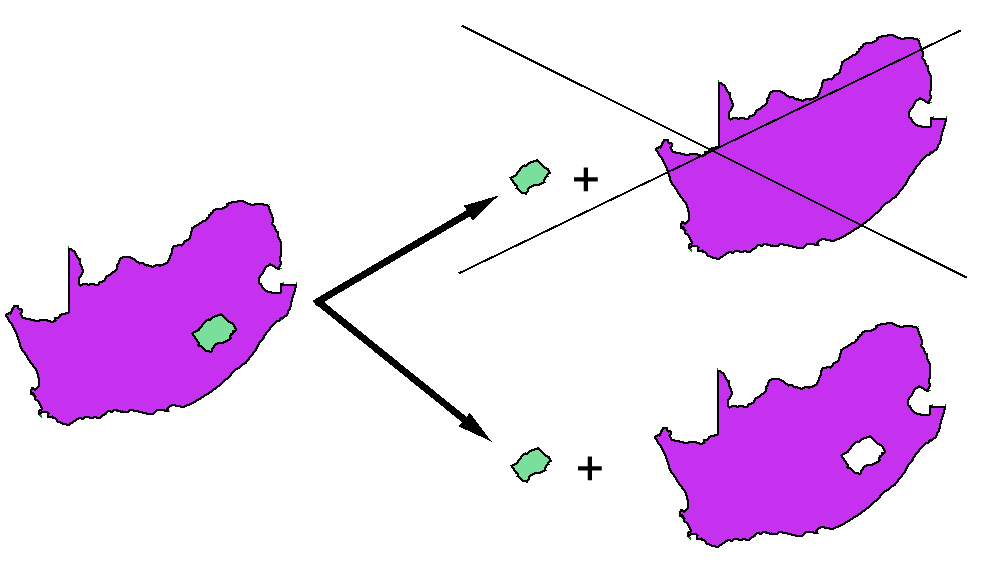
\includegraphics[width=.6\textwidth]{Tipos_datos/Poligonos_con_huecos.png}
\caption{\small Los huecos de un pol�gono han de considerarse como parte de este.}
\label{Fig:Poligonos_con_huecos} 
\end{figure}

En realidad, los huecos se registran como pol�gonos disjuntos que pertenecen a la entidad, aunque en lugar de representar un territorio que se a�ade, representan uno que se <<quita>>. Una forma habitual de hacer esto es almacenar las coordenadas de los v�rtices de estos pol�gonos interiores en sentido inverso, de tal modo que su �rea es negativa. De esta forma, la suma total del �rea de los pol�gonos de la entidad es igual al �rea buscada\footnote{La f�rmula empleada para el c�lculo del �rea de un pol�gono se expone en la p�gina \pageref{Eq:Area_poligono}}.

\index{Pol�gono!�rea de}

Dentro de un SIG, una capa vectorial puede contener un �nico tipo de primitiva. As�, tenemos capas vectoriales de puntos, de l�neas y de pol�gonos, respectivamente. La elecci�n de uno u otro tipo de capa para registrar una variable o conjunto de ellas ha de ser funci�n del tipo de fen�meno que se pretende modelizar con dicha capa o la precisi�n necesaria, entre otros factores. 

Por ejemplo, una capa de puntos puede representar un conjunto de ciudades, cada una de ellas definida como un �nico punto. Sin embargo, puede emplearse una capa de pol�gonos y no recoger una �nica coordenada (correspondiente, por ejemplo, al centro de la ciudad), sino el contorno o los l�mites administrativos de esta. Dependiendo del caso, ser� m�s apropiado elegir una u otra alternativa.

De igual modo, la capa de v�as representada en la figura \ref{Fig:Vias_modelos_representacion} es una capa de l�neas. Cada l�nea, como elemento te�rico de ancho nulo, representa el eje de la v�a. Si se requiere una mayor precisi�n en la definici�n de la superficie de rodadura de dichas v�as, una capa de pol�gonos puede ser utilizada en lugar de una de l�neas.

Lo anterior tiene una evidente relaci�n con los conceptos de escala\index{Escala} y generalizaci�n\index{Generalizaci�n!cartogr�fica} que vimos en el cap�tulo \ref{Fundamentos_cartograficos}.

No debe pensarse que las capas vectoriales, sean del tipo que sean, se emplean �nicamente para recoger fen�menos o elementos cuya forma coincide con la de las primitivas geom�tricas (es decir, puntos para recoger elementos puntuales, l�neas para aquellos elementos con una dimensi�n mucho menor que la otra, y pol�gonos para el caso de superficies). Adem�s de los ejemplos anteriores, debemos recordar que el modelo vectorial tambi�n sirve para representar campos y recoger variables tales como la elevaci�n.

As�, en los ejemplos de la figura \ref{Fig:MDE_modelos_representacion} encontramos capas de puntos, lineas (curvas de nivel) y pol�gonos (TIN), todas ellas empleadas para representar la variable elevaci�n. En ocasiones se emplean las primitivas para recoger objetos reales de forma similar, mientras que en otros casos sirven para plantear un modelo l�gico y recoger variables que no se asemejan de modo alguno a las formas geom�tricas registradas.

A prop�sito de la capa de puntos regulares, cabe pensar que es similar en concepto y forma a la malla r�ster, ya que es regular. Sin embargo, existen dos diferencias importantes: en primer lugar, en la capa de puntos hay zonas en blanco, de las que no sabemos su elevaci�n, mientras que en la malla r�ster las celdas tienen una superficie y cubren en su conjunto todo el espacio. En segundo lugar, si tenemos esa capa de puntos en un SIG, esta va a contener las coordenadas particulares de cada punto, ya que en s� las capas vectoriales no son regulares (pueden guardar alguna regularidad, pero no necesariamente), y por tanto es necesario, como hemos visto, registrar expl�citamente sus coordenadas. De modo similar podr�amos hacer una capa de pol�gonos cuadrados, pero seguir�a sin ser una malla r�ster, m�s a�n si careciera de un elemento que veremos en breve: la topolog�a. \index{Topolog�a}

\subsubsection{La componente tem�tica en el modelo vectorial}

La forma en la que los modelos de representaci�n separan las dos componentes de la informaci�n geogr�fica hemos visto que es bien distinta. En el modelo r�ster se tiene un conjunto de valores (la componente tem�tica), los cuales guardan una estructura dada, la cual por s� misma establece su disposici�n en el espacio (la componente espacial). En el vectorial, por su parte, la componente espacial se recoge expl�citamente seg�n una serie de puntos, la cual puede ser m�s o menos compleja en funci�n de la complejidad de la entidad a representar o el detalle con que se recoja. A este conjunto de puntos se le relaciona despu�s con una serie de valores, que son los que definen las propiedades de la entidad.

Estos valores, los \emph{atributos}, a diferencia del caso r�ster, suelen ser m�ltiples. Por ejemplo, dada una capa vectorial de pa�ses, podemos recoger valores asociados a cada pa�s tales como su superficie, su poblaci�n, el Producto Interior Bruto, el nombre de su capital o el idioma que se habla. Todo este conjunto de valores se asocian a una �nica copia de la componente espacial, y esta no debe repetirse para recoger cada uno de esos par�metros. En el modelo r�ster, si tenemos $n$ capas distintas, en realidad estamos almacenando $n$ veces la componente espacial.
\index{Atributos!de una capa vectorial}

Por esta estructura particular, la componente tem�tica se presta especialmente a almacenarse en una base de datos, siendo en la actualidad las m�s extendidas las denominadas \emph{bases de datos relacionales}. Estas bases de datos se \emph{enlazan} a la componente espacial y permiten una serie de operaciones(ver cap�tulo \ref{Consultas}) y un manejo ventajoso de los \emph{atributos}. Existen, por tanto, dos realidades: la relativa a la componente geogr�fica y la base de datos que gestiona los atributos, la cual permite an�lisis y operaciones independientes, del mismo modo que si no existir� una localizaci�n asociada a dichos atributos. Estas realidades pueden estar muy separadas, gestion�ndose en aplicaciones distintas y almacen�ndose en ficheros diferentes, con lo cual existe una divisi�n formal mucho m�s acusada que en el caso de las capas r�ster, que se asemejan m�s a unidades de informaci�n autocontenidas.

En el caso de las capas r�ster, no es necesario recurrir a una base de datos, y simplemente la representaci�n del conjunto de valores de la variable en las distintas celdas sirve para el almacenamiento, an�lisis y manejo de la informaci�n. Como indica \cite{Heywood1998Longman}, esta forma de \emph{conectar} las componentes espacial y tem�tica es apta para el an�lisis, pero el manejo de los atributos requiere la presencia de una base de datos.\index{Base de datos}

El establecimiento de las bases de datos, su manejo y su implementaci�n dentro de un SIG es un tema altamente complejo. La forma en que el manejo de la componente tem�tica y la gesti�n de la base de datos se establecen, as� como la imbricaci�n de la una en la otra, es la materia exclusiva del cap�tulo \ref{Bases_datos}, donde todos estos temas se desarrollar�n con profundidad.

\subsubsection{Topolog�a}
\label{Topologia}

\index{Topolog�a}

Un elemento particular del modelo de representaci�n vectorial es la \emph{topolog�a}. En t�rminos matem�ticos la topolog�a estudia las caracter�sticas de los objetos geom�tricos que no var�an al aplicar una transformaci�n topol�gica tal como, por ejemplo, una transformaci�n af�n\index{Transformaci�n!af�n}. Si tomamos un mapa y lo distorsionamos, los �ngulos, las superficies y las distancias se ven afectadas. Sin embargo, otras propiedades tales como la adyacencia entre elementos o las relaciones entre estos se conservan. Por ejemplo, si una ciudad est� dentro de una determinada provincia en un determinado mapa, no existe forma de distorsionar esta para lograr que dicha ciudad se encuentre fuera de la provincia.

En el �mbito de los SIG se entiende la topolog�a desde un punto de vista menos estricto y m�s funcional. En general, se dice que una capa de informaci�n tiene topolog�a si en ella se almacenan de alg�n modo las relaciones entre los distintos elementos que la componen. En caso contrario, la capa es de tipo puramente cartogr�fico, ya que los elementos que contiene no presentan relaci�n entre s�, o al menos esta relaci�n no est� almacenada junto a la propia informaci�n de estos elementos.

En una capa r�ster, las relaciones topol�gicas vienen impl�citas en el propio modelo r�ster, y son ajenas a la informaci�n como tal, dependiendo de la estructura de la malla de datos en s�. En el modelo vectorial, sin embargo, se recoge la informaci�n relativa a cada elemento de forma individual, y si las relaciones existentes no se registran de modo explicito, no se tendr� posteriormente informaci�n sobre ellas.

Disponer de topolog�a en una capa vectorial es de gran importancia a la hora de llevar a cabo ciertos tipos de an�lisis, as� como otros tales como la edici�n de los propios datos geogr�ficos. La topolog�a no aporta beneficio a la hora de representar una capa, pero s� a la hora de llevar a cabo an�lisis sobre ella \cite{Herring1987Autocarto}. 

En la figura \ref{Fig:Topologia_edicion} se puede observar la diferencia existente entre editar una capa de pol�gonos con topolog�a y una sin ella. En el primer caso, la informaci�n contenida en la capa antes de su edici�n nos informa no solo de la forma de cada pol�gono, sino tambi�n del hecho de que ciertos pol�gonos comparten bordes comunes y de que el conjunto de ellos cubre el espacio de forma completa (constituyen una teselaci�n\index{Teselaci�n}). As�, al modificar un punto en uno de los pol�gonos, todos aquellos pol�gonos adyacentes que comparten dicho punto modifican tambi�n su per�metro. Las capacidades de edici�n implementadas en el Sistema de Informaci�n Geogr�fica hacen uso de la informaci�n topol�gica a la hora de editar geometr�as. En el segundo caso, sin embargo, esta informaci�n no existe, y no se pueden alterar los pol�gonos adyacentes, perdi�ndose la teselaci�n completa del espacio.

\begin{figure}[!hbt]   
\centering
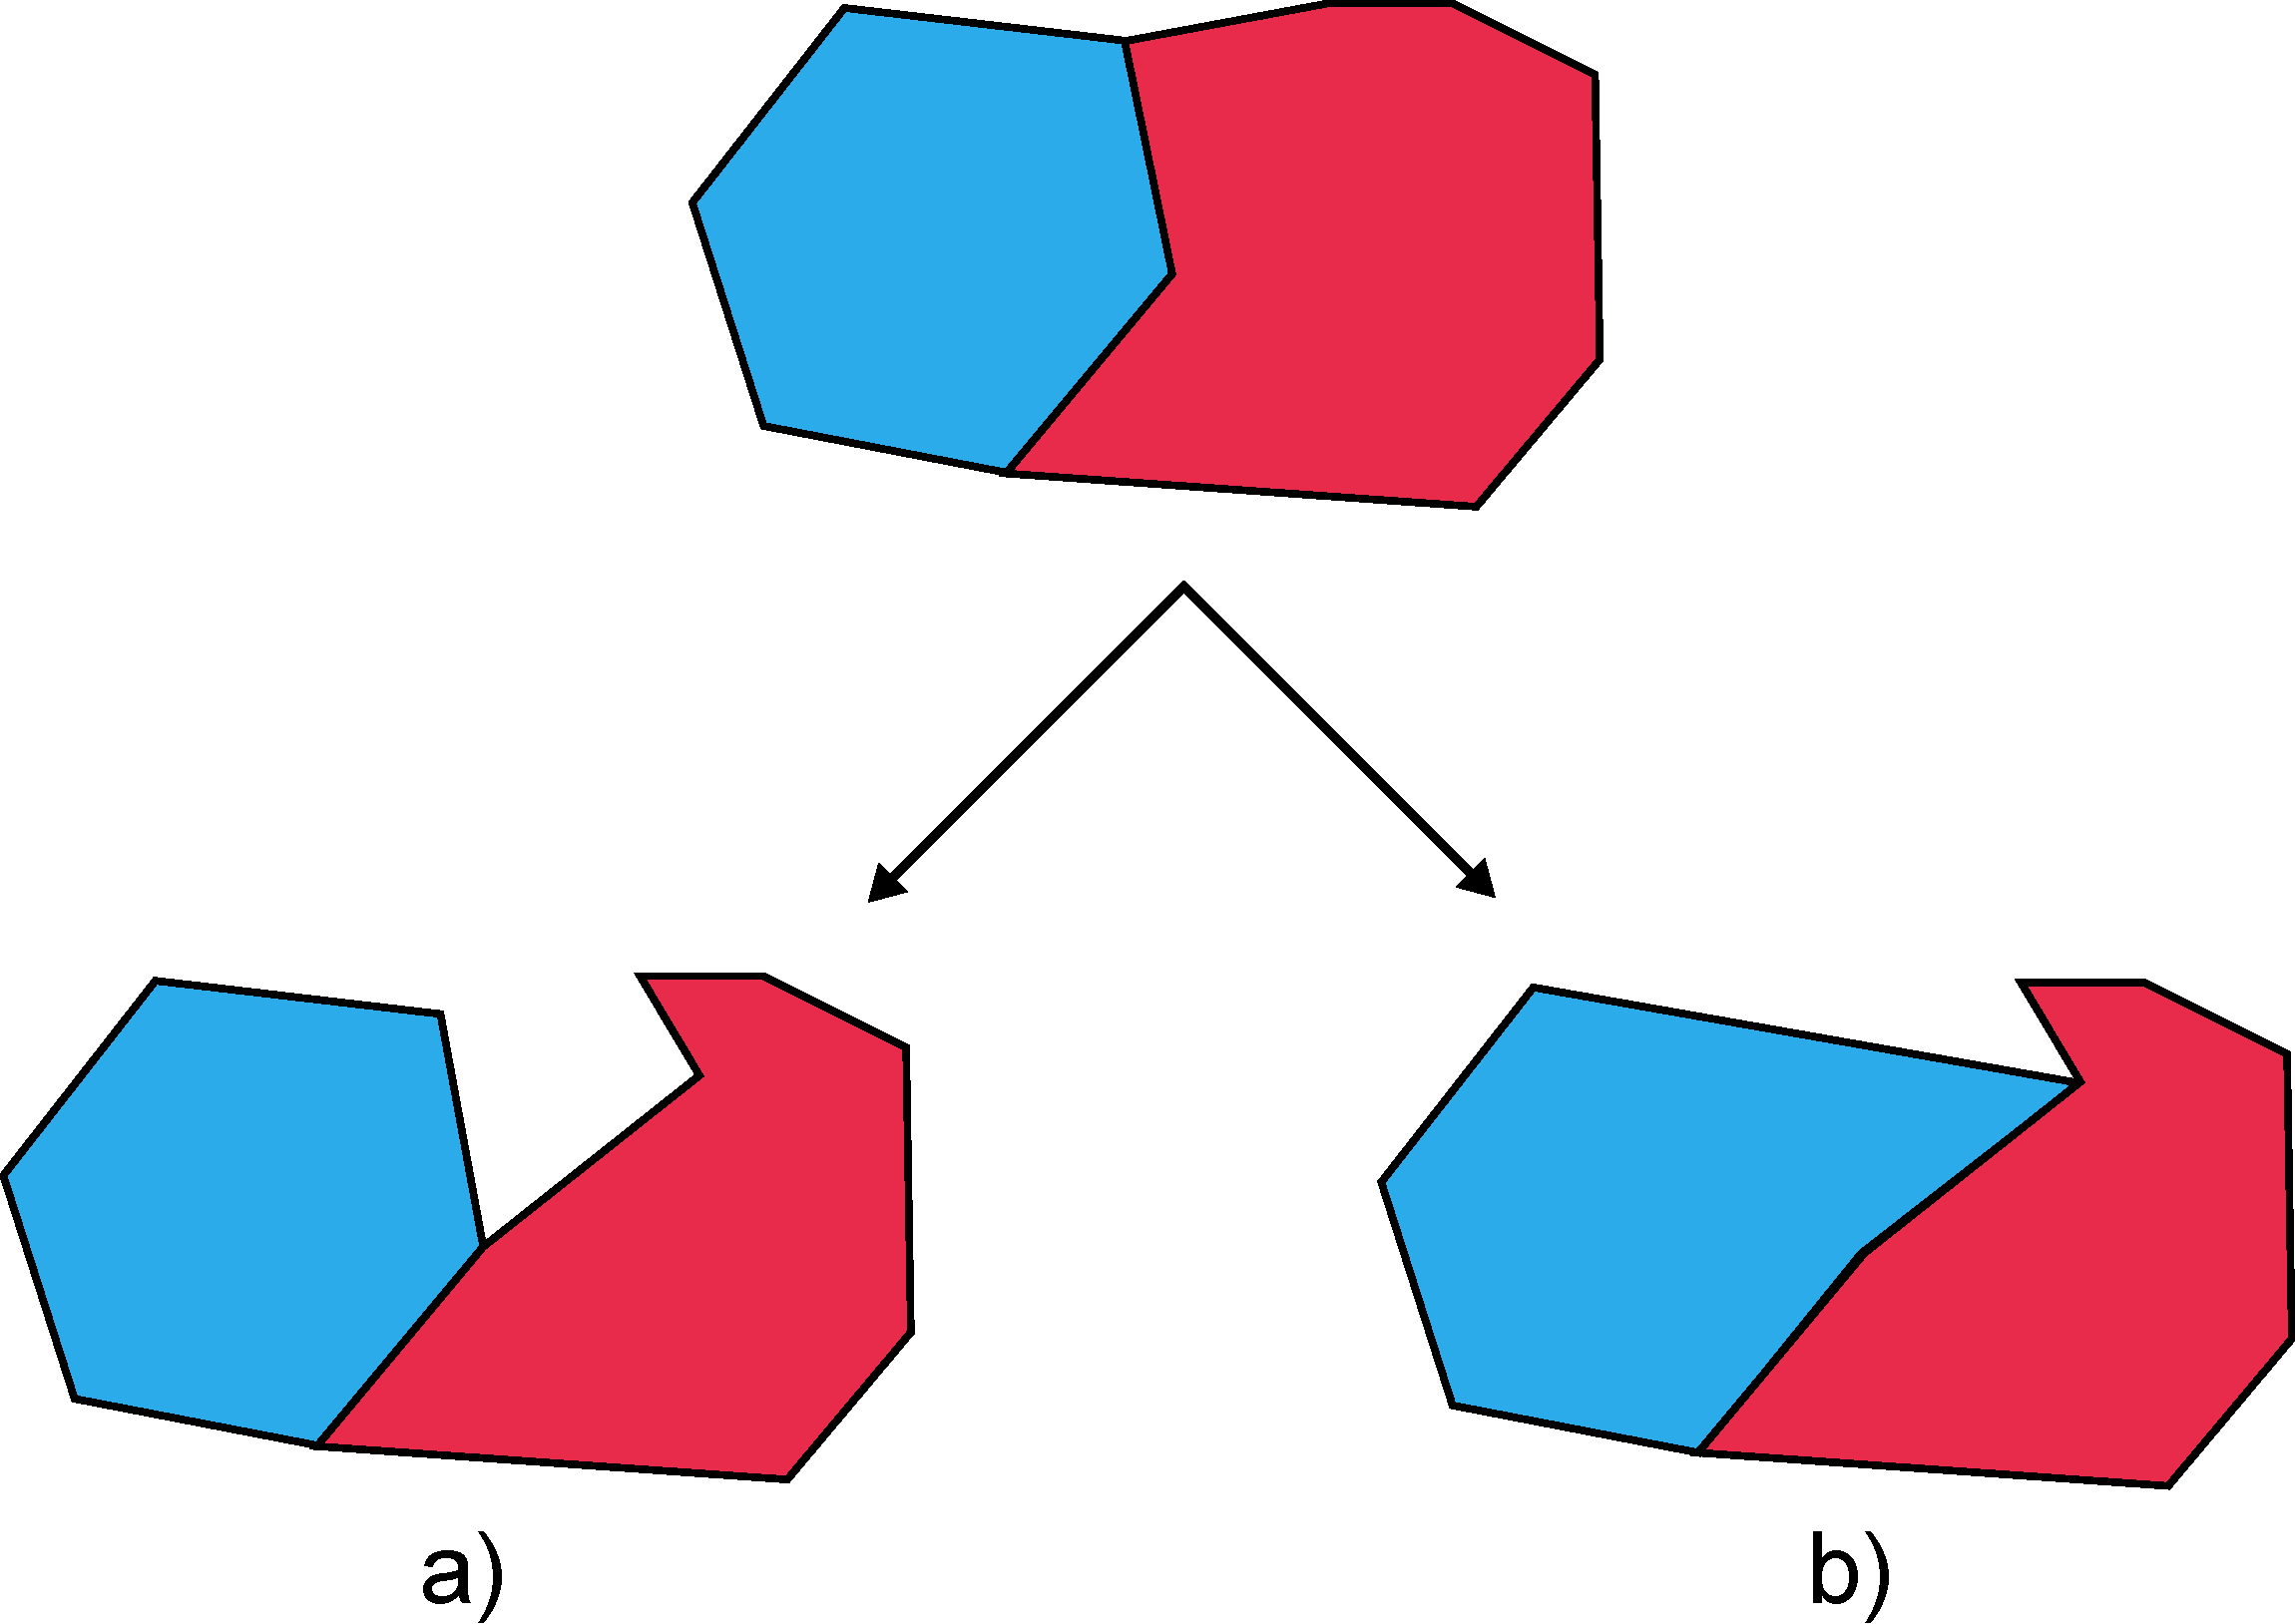
\includegraphics[width=.6\mycolumnwidth]{Tipos_datos/Topologia_edicion.pdf}
\caption{\small Diferencias entre la edici�n (desplazamiento de un punto) no disponiendo de topolog�a (a) o con ella (b).}
\label{Fig:Topologia_edicion} 
\end{figure}

La topolog�a es en este caso un elemento que contribuye a la calidad de los datos, pues mantiene la coherencia espacial de estos y evita la aparici�n de elementos tales como pol�gonos de muy peque�o tama�o, frecuentes en la digitalizaci�n de entidades debido a las peque�as imprecisiones que se presentan en el proceso, y que causan la presencia de falsos solapes entre pol�gonos.

No obstante, no todos los SIG incorporan capacidades de manejo y an�lisis de capas vectoriales con topolog�a, y son menos a�n los que implementan capacidades para crear dicha topolog�a. En general, estas han quedado reservadas a las aplicaciones de alta gama, y el manejo de informaci�n vectorial en los SIG de escritorio no incluye de forma general lo relativo a la topolog�a.

Otro ejemplo de proceso en el que se hace necesario el disponer de capas con topolog�a es el an�lisis de redes (este se detalla en el cap�tulo\index{Redes!an�lisis de} \ref{Analisis_redes}). Un mero conjunto de elementos geom�tricos (l�neas en este caso), no nos da informaci�n sobre los posibles enlaces entre las v�as que quedan representadas. Los puntos donde se cruzan dos v�as pueden ser cruces o rotondas (es decir, puede pasarse de una v�a a otra, existiendo conexi�n entre ellas), o bien pasos elevados o subterr�neos donde una de las v�as pasa por encima de la otra (y por tanto no existe comunicaci�n entre ambas). Las circunstancias son muy distintas en funci�n del tipo de cruce que exista, y por ello es imprescindible conocer esta informaci�n para efectuar un an�lisis de redes correcto. 

Otro elemento que no se puede recoger sin topolog�a son las direcciones de circulaci�n. Habr� v�as que puedan recorrerse en ambos sentidos, mientras que habr� otras que solo permitan movimiento de tr�fico en una direcci�n. Saber en qu� direcci�n podemos recorrer una v�a es vital para poder plantear cualquier tipo de an�lisis, y esta es una informaci�n de la que no disponemos si nuestra red viaria no ha sido representada mediante un modelo con topolog�a.

Estas circunstancias se recogen de forma esquem�tica en la figura \ref{Fig:Topologia_vias}

\begin{figure}[!hbt]   
\centering
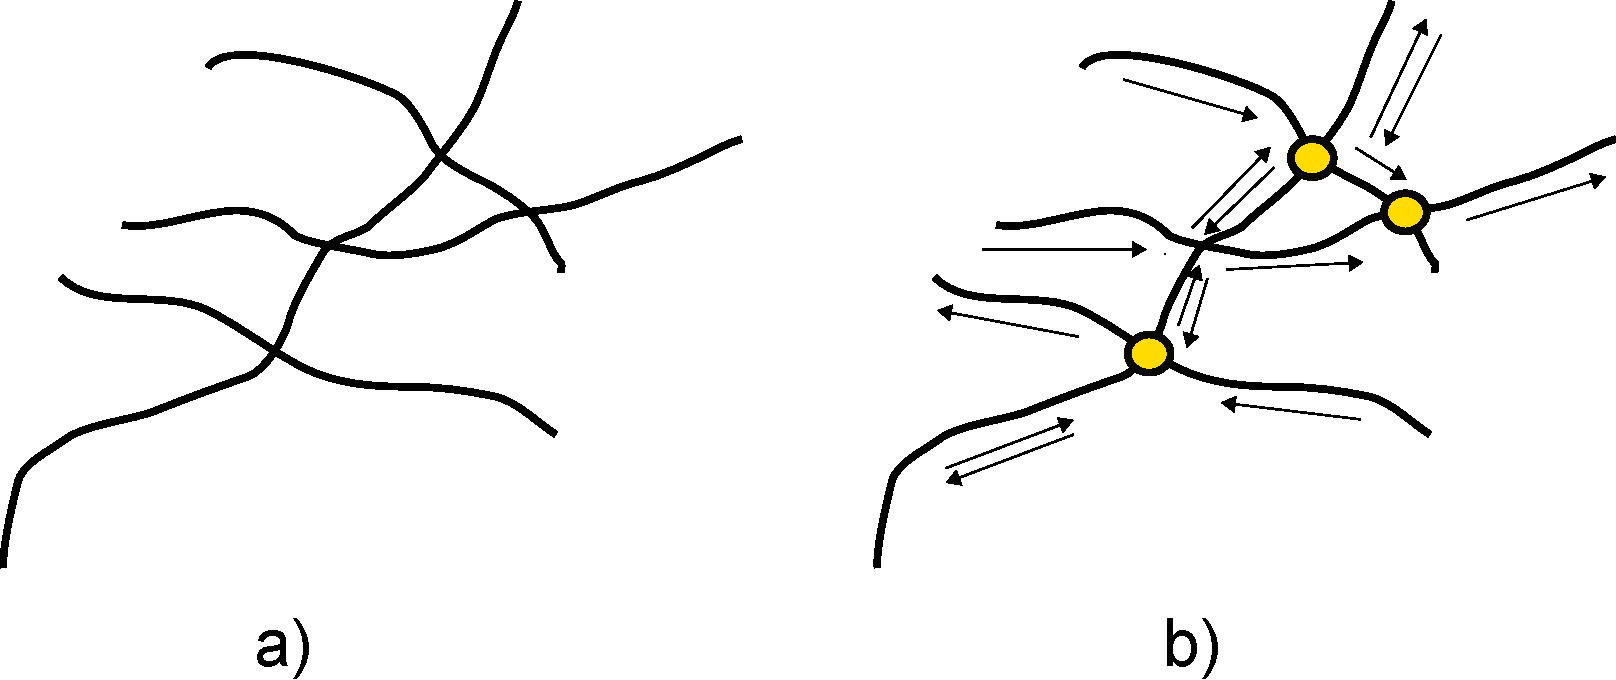
\includegraphics[width=.6\mycolumnwidth]{Tipos_datos/Topologia_vias.pdf}
\caption{\small Capa de v�as de comunicaci�n sin topolog�a (a) o con ella (b). Los puntos en este segundo caso indican conexiones entre vias, y son una representaci�n visible de la topolog�a existente. Las flechas indican la direcci�n de circulaci�n y, al igual que sucede con las conexiones, solo est�n presentes si existe topolog�a}
\label{Fig:Topologia_vias} 
\end{figure}


Aunque, como se ha mencionado, las capas r�ster en cierta forma contienen informaci�n topol�gica (se conoce la relaci�n de adyacencia entre las distintas celdas), esta es \emph{d�bil}, y no suficiente para an�lisis complejos como el de redes donde existen distintos elementos como los mencionados cruces o las direcciones de circulaci�n. Aparte de la inherente peor disposici�n del modelo de representaci�n para recoger una entidad espacial tal como una red, el modelo r�ster no es �ptimo para recoger la necesaria informaci�n topol�gica al respecto. Existen algunos intentos de adaptarlo a estas circunstancias (v�ase, por ejemplo \cite{Husdal2000MsC}), pero en general no se encuentran implementados de forma habitual.

\index{Topolog�a!sobre capas r�ster}

\subsubsection{Modelo vectorial sin topolog�a (\emph{spaguetti})}

\index{Spaguetti@\emph{Spaguetti}}

El modelo de datos vectorial almacena la informaci�n geogr�fica mediante una serie de entidades geom�tricas (lineas, puntos, pol�gonos), y una informaci�n asociada (los atributos). La forma en que estas geometr�as se recogen es, no obstante, �nica, y en funci�n del enfoque adoptado, permitir� el almacenamiento o no de propiedades topol�gicas relativas a dichas geometr�as. Se tienen as� \emph{submodelos} de representaci�n, cada uno de ellos con un esquema distinto de almacenamiento de los elementos individuales que constituyen una capa r�ster.

Con independencia del submodelo, en todo caso las entidades se recogen mediante las coordenadas de sus puntos, pues como ya se vio toda entidad es reducible a un conjunto de puntos. La diferencia estriba en la forma en que dichos puntos se asocian a la representaci�n de una entidad dada. Para el caso de una capa de puntos, no existe diferencia alguna, pero en el caso de l�neas o pol�gonos s� la hay.

En el tipo m�s simple, se recogen �nicamente las propiedades geom�tricas de cada entidad, almacenando para cada una de ellas el conjunto de puntos individuales que la componen. Esto aporta toda la informaci�n necesaria sobre la entidad, pero deja de lado la topolog�a. Algunas propiedades topol�gicas pueden calcularse, tales como saber si un punto esta contenido dentro de un pol�gono o si dos rectas se cruzan, pero para otras no se dispone de informaci�n suficiente. As�, aunque podamos saber si dos l�neas se cruzan, no podemos saber si este cruce implica una conexi�n real entre ellas de forma que pueda pasarse de la una a la otra o no, como vimos en la figura \ref{Fig:Topologia_vias}.

Esta forma de recoger las entidades vectoriales es similar a la que encontramos en un mapa cl�sico, en el cual podemos conocer la forma de un �rea dada o el recorrido que sigue una determinada carretera, pero no las relaciones existentes. �nicamente disponemos del trazo con el que se han dibujado estos elementos. Por esta raz�n, y como se ha dicho, un modelo vectorial sin topolog�a es perfectamente v�lido para la representaci�n de cualquier tipo de informaci�n en formato vectorial, pero no tanto para su an�lisis.

El almacenamiento de entidades basado en una mera lista de coordenadas de cada entidad se conoce popularmente como \emph{spaghetti}, pues si pensamos en una capa de lineas sin topolog�a que se entrecruzan en el espacio, esta se asemejan en cierta forma a un ca�tico plato de \emph{spaguettis} sin orden ni relaci�n entre ellos.

La mayor ventaja de este modelo es su simplicidad, raz�n por la cual es la habitual en muchos de los SIG m�s populares. Para muchos usuarios, es suficiente trabajar con datos vectoriales sin topolog�a, pues las labores frecuentes que desarrollan, tales como consultas (cap�tulo \ref{Consultas}) o creaci�n de mapas derivados, no requiere conocer las relaciones topol�gicas existentes.\index{Consultas}

Gran parte de las operaciones que se desarrollan en un SIG no requieren topolog�a, y por ello no es necesario asumir siempre el coste que implica trabajar con ella (mayor complejidad en general). Es por ello que incluso aquellos SIG que s� poseen la capacidad de trabajar con topolog�a, tambi�n disponen de formas de trabajar sin ella, empleando datos que carecen de topolog�a. Esto es as� tambi�n debido a que mucha informaci�n disponible no incluye topolog�a, ya que o bien esta no se incorpor� en el momento de la digitalizaci�n, o bien el formato de fichero en el que se almacen� no soportaba la inclusi�n de topolog�a. 

En otros casos, la propia naturaleza de la variable que recogemos puede requerir ser almacenada sin topolog�a, o bien puede ser que no existan relaciones topol�gicas que representar. Una capa de pol�gonos en las cuales se recojan las �reas de influencia de unos determinado fen�menos puntuales pueden perfectamente solaparse. No existe en este caso esa relaci�n que hace que el conjunto de pol�gonos que las representan cubra la totalidad del espacio y cada punto pertenezca a una sola entidad. En este caso, un punto puede estar afectado por uno, varios o ninguno de dichos fen�menos puntuales, y por tanto pertenecer a una, varias o ninguna de las entidades poligonales que representan sus respectivas �reas de afecci�n. Al modificar una de ellas (por ejemplo, si el fen�meno puntual que la origina var�a su intensidad), las dem�s geometr�as no deber�an verse afectadas. No existe como tal una relaci�n que deba recogerse en forma de topolog�a.

\subsubsection{Con topolog�a}

La alternativa al modelo vectorial sin topolog�a (el que denomin�bamos \emph{spaguetti}) es el almacenamiento expl�cito de las relaciones topol�gicas, recogiendo las coordenadas de los puntos que constituyen cada entidad, pero no mediante una simple lista para cada una de ellas. Recogiendo de forma individual toda la informaci�n espacial correspondiente a cada entidad, la topolog�a se pierde, pues no se considera al conjunto de entidades como un conjunto en el cual existen relaciones internas, sino como una simple colecci�n de cosas. Para recoger la topolog�a es necesario considerar todos los puntos que constituyen las entidades, y despu�s \emph{formar} las entidades a partir de ese todo de puntos, considerando en el proceso que un mismo punto puede pertenecer a varias entidades. Esto es lo que se denomina frecuentemente un \emph{diccionario de puntos}, ya que contiene las definiciones de estos (sus coordenadas) y en base a ellos se construyen las distintas geometr�as. \index{Diccionario de puntos}

Esta forma de considerar el conjunto de entidades evita, adem�s, la redundancia en los datos.\index{Redundancia} Por ejemplo, para el caso mostrado en la figura \ref{Fig:Topologia_edicion}, y en caso de no tener topolog�a, el punto que es movido est� almacenado dos veces, una por cada pol�gono. Al desplazarlo, solo se modifica una copia de dicha coordenada, la que pertenece al pol�gono editado, mientras que la otra permanece en su lugar. Si se dispone de topolog�a, este punto se almacena una �nica vez, y al desplazarse se modifican las fronteras de todos los elementos (lineas o pol�gonos, seg�n el caso) cuya frontera incluye dicho punto.

La denominaci�n de \emph{diccionario de puntos} que se mencionaba anteriormente es muy reveladora en este sentido. Si los puntos son como las palabras de un diccionario y los pol�gonos como frases o p�rrafos, basta pensar en lo poco pr�ctico que ser�a escribir una frase en la que debiera definirse cada palabra al introducirla en dicha frase. Resulta mucho m�s adecuado (y ahorra esfuerzos al escritor), utilizar las palabras simplemente, y despu�s definir estas en un diccionario en caso de que el lector no las conozca y necesite una referencia. Con el caso de los puntos sucede algo similar.

Existen diversos modelos para almacenar tanto las propias geometr�as como sus relaciones inherentes, dos de los cuales se muestran en la figura \ref{Fig:Modelos_topologia} mediante sendos ejemplos en los que se codifican pol�gonos y l�neas.

\begin{figure}[!hbt]   
\centering
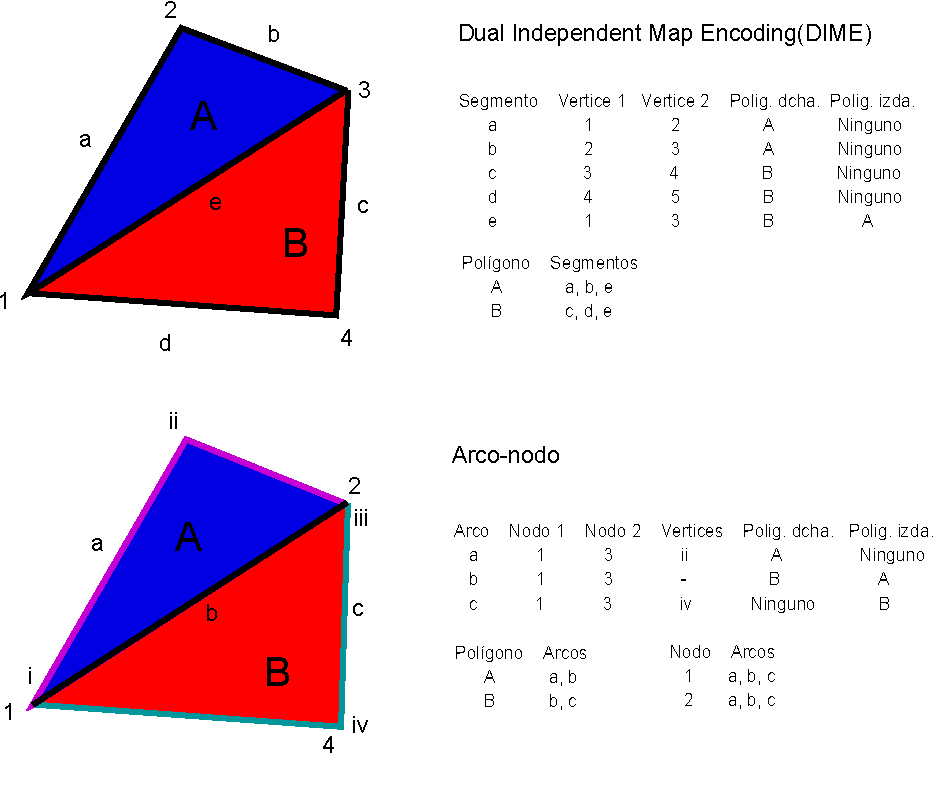
\includegraphics[width=.8\textwidth]{Tipos_datos/Modelos_topologia.pdf}
\caption{\small Dos modelos para representar la topolog�a de l�neas y pol�gonos. a) DIME, b) arco--nodo.}
\label{Fig:Modelos_topologia} 
\end{figure}

El primero de estos modelos es un modelo de car�cter hist�rico denominado DIME (\emph{Dual Independent Map Encoding})\index{Dual Independent Map Encoding}, desarrollado originalmente por el \emph{US Bureau of the Census}\index{US Bureau of the Census}, y posteriormente mejorado en el modelo TIGER, empleado para la digitalizaci�n de cartograf�a urbana. El segundo es el modelo \emph{arco--nodo}, probablemente el m�s difundido y popular en la actualidad, aunque a este respecto los planteamientos existentes son muy variados.\index{Modelo!arco--nodo}

En este modelo existen dos unidades fundamentales: Los nodos, que son puntos donde se \emph{conectan} varias l�neas; y los \emph{arcos}, que son lineas entre dos nodos. Estas l�neas no han de ser rectas, ya que pueden contener en su recorrido \emph{v�rtices}. Los v�rtices son en realidad los puntos que solo pertenecen a una entidad, mientras que los nodos pertenecen a varias de ellas.\index{V�rtices}\index{Arco}

Una capa de l�neas se describe como un conjunto de arcos y nodos, de forma que, atendiendo a los nodos como enlaces entre las l�neas, se pueden conocer las relaciones entre ellas. En el caso de pol�gonos, estos se forman con conjuntos de arcos que delimitan las fronteras. Los pol�gonos que son adyacentes comparten uno o m�s arcos, quedando establecida as� mediante ellos la relaci�n topol�gica.

En el caso del modelo DIME, sin embargo, vemos que cada linea recta entre dos puntos se trata como una unidad, es decir, que todos los v�rtices son considerados como nodos y los arcos se componen siempre de una sola l�nea. El arco es en realidad un segmento. En ambos casos, no obstante, cada arco tiene un inicio y un final ---y por tanto una direcci�n---, y puede definirse un lado derecho y otro izquierdo seg�n se avanza en dicha direcci�n. Como puede verse, tambi�n en ambos modelos se recoge expl�citamente qu� pol�gono, en caso de haber alguno, se sit�a a cada lado del arco.

La informaci�n que se recoge seg�n estos modelos, vemos que se divide en bloques seg�n los distintos niveles, desde los puntos, que han de recogerse en un diccionario de puntos (aunque este no queda reflejado en las tablas de la figura), pasando por los segmentos o arcos, y hasta los pol�gonos, definidos estos en base a los anteriores.

Con independencia del modelo, y sin entrar en m�s detalles, todos estos elementos en conjunto sirven para recoger las relaciones existentes entre los elementos, de tal modo que pueden llevarse a cabo tambi�n aquellas operaciones que no dependen exclusivamente de la posici�n, sino asimismo de otra serie de propiedades.

Dentro de los modelos existentes, encontramos asimismo variaciones en funci�n de la tarea principal que se desee realizar. La eficiencia de cierto tipo de c�lculos puede aumentarse notablemente si se elige un modelo de representaci�n �ptimo, como podemos ver si analizamos una de las operaciones m�s comunes: el c�lculo de rutas �ptimas entre dos puntos (los detalles sobre este c�lculo se exponen en el cap�tulo \ref{Costes}, aqu� por el momento �nicamente mostraremos sus implicaciones en los modelos de representaci�n).


\index{Ruta �ptima}

Para calcular la ruta �ptima entre dos puntos dados de una red necesitamos conocer qu� nodos de la red est�n conectados entre s� y por qu� v�as est�n conectados, ya que las caracter�sticas de estas condicionan el movimiento. La informaci�n necesaria para este c�lculo puede almacenarse perfectamente seg�n un modelo arco--nodo como el que ya conocemos, pero considerando las particularidades del an�lisis que queremos realizar, existen otros modelos m�s apropiados. 

Por ejemplo, se puede tener en cuenta que los v�rtices de un nodo no tienen relevancia alguna. Si el tr�nsito se realiza entre dos nodos, a efectos del c�lculo es indiferente que el tramo que los une tenga unos u otros v�rtices. Lo �nico que importa es saber que existe un tramo que los conecta y las caracter�sticas de ese tramo como, por ejemplo, el tiempo que cuesta recorrerlo o si conecta el nodo A con el B y el B con el A o solo lo hace en una de las direcciones anteriores. Por ello, en el caso del an�lisis de redes, la clave reside en almacenar de forma eficiente los nodos y las relaciones, pues estos son los elementos esenciales para efectuar los c�lculos

Algunos modelos empleados com�nmente para el almacenamiento de redes son los siguientes \cite{NCGIA}:

\begin{itemize}
\item Matriz de incidencias arco--nodo
\item Matriz de adyacencias nodo--nodo
\item Listas de adyacencia
\item Estrella directa e inversa\footnote{Forward and reverse star}
\end{itemize}

\index{Matriz!de incidencias}\index{Matriz! de adyacencias}\index{Listas de adyacencia}\index{Estrella directa e inversa}\index{Forward and reverse star}

La matriz de adyacencias nodo--nodo es sumamente sencilla, ya que simplemente, para un n�mero $n$ de nodos, contiene una matriz de tama�o $n\times n$, en la que cada elemento ($i,j$) indica la existencia o no de conexi�n entre los nodos $i$ y $j$ y la naturaleza de dicha conexi�n. Si el elemento es igual a cero indica que no existe posibilidad de desplazarse directamente del nodo $i$ al nodo $j$. En caso contrario, el valor es igual a la propiedad que se desee recoger del tramo, por ejemplo el tiempo que se tarda en recorrer o la velocidad m�xima a la que puede hacerse ese recorrido.

La gran ventaja de este m�todo es su gran sencillez, que deriva en sencillas implementaciones de los algoritmos correspondientes.

El m�todo de estrella directa e inversa, por su parte, no es tan sencillo (una descripci�n algo m�s detallada puede encontrarse en \cite{NCGIA}), pero, no obstante, es el m�s eficaz \cite{Ahuja1993Prentice}, y sus tiempos de c�lculo asociados son los menores de entre todos los anteriores. 

M�s all� de los detalles particulares del modelo de representaci�n, lo importante es tener presente que existen diversas formas de representar el dato geogr�fico, y que cada una de ellas tiene sus ventajas e inconvenientes en relaci�n con la funci�n que los datos hayan de desempe�ar.

\subsubsection{TIN}
\label{TIN}

Hemos visto c�mo una capa vectorial con topolog�a nos sirve para modelizar ventajosamente elementos como una red de v�as o una teselaci�n\index{Teselaci�n} del espacio en, por ejemplo, diferentes clases de usos de suelo. Adem�s de esto, la incorporaci�n de topolog�a sirve para mejorar la representaci�n de campos mediante modelos vectoriales, permitiendo la aparici�n de modelos como los TIN, ya presentados con anterioridad. 

Un TIN\index{Triangulated Irregular Network (TIN)} \cite{Peuker1978ASP} es una red formada por un conjunto de tri�ngulos interconectados, cada uno de los cuales representa a una zona de caracter�sticas homog�neas en lo que a la variable estudiada respecta. Debido a esto, y como puede verse en la figura \ref{Fig:MDE_modelos_representacion}, el n�mero de tri�ngulos var�a seg�n las caracter�sticas propias de la zona. 

En aquellos lugares en los que se d� una gran variaci�n (en caso de recoger el relieve ser� en las �reas m�s abruptas), se utiliza un gran n�mero de tri�ngulos para recoger toda esa variabilidad. Cuando, por el contrario, los valores no var�an de forma tan notable (zonas de relieve m�s llano), pueden emplearse menos tri�ngulos. Puesto que cada tri�ngulo est� formado, como todo pol�gono, por puntos, podemos decir que se necesitan menos puntos para almacenar un terreno si este es llano que si este es muy abrupto.

Cada tri�ngulo tienen unas propiedades constantes, como corresponde al modelo vectorial. En particular, se considera habitualmente que todos los puntos dentro de un mismo tri�ngulo constituyen un plano, con una pendiente y una orientaci�n fija por tanto.

La topolog�a del modelo permite llevar a cabo an�lisis diversos sobre un TIN, ya que para cada tri�ngulo se tiene conocimiento de cu�les son los adyacentes a este, y es en el an�lisis de dichos adyacentes en el que se basan gran parte de los algoritmos. Este an�lisis resulta sencillo de implementar en una capa r�ster, pues la propia estructura de la misma informa directamente de las celdas circundantes, pero en el caso vectorial requiere la presencia de topolog�a para plantear un esquema similar de operaci�n. 

El an�lisis de los TIN no se desarrolla en detalle en este libro, pero resulta interesante recalcar en este punto que resulta posible de igual modo, y ello es debido a la presencia de topolog�a en la propia estructura del modelo de representaci�n.

Las particularidades del TIN hacen que existan sub--modelos principales para almacenar el conjunto de tri�ngulos, distintos del habitual arco--nodo, y pensados espec�ficamente para responder a las necesidades que los TIN demandan como modelos vectoriales para representar variables continuas (en este sentido, es algo muy similar al caso que ve�amos anteriormente de las redes). Estos modelos son dos, principalmente:

\begin{itemize}
 \item Almacenamiento de los tri�ngulos uno por uno, cada uno con las coordenadas de todos sus tres puntos (coordenadas tridimensionales, no planas) y un c�digo de identificaci�n, y almacenamiento de los c�digos de los tri�ngulos adyacentes.
\item Almacenamiento de los v�rtices y un c�digo para cada uno de ellos, as� como los c�digos de los v�rtices a los que se encuentra conectado, en un orden establecido (horario o antihorario).
\end{itemize}

M�s informaci�n sobre TIN puede encontrarse en \cite{Mark1975GA}. La creaci�n de TIN se trata con m�s detalle en el cap�tulo \ref{Creacion_capas_vectoriales}.

\subsection{Raster \emph{vs} vectorial}

Resulta obvio que las diferencias entre los modelos r�ster y vectorial son muy notables, y que cada uno de ellos posee sus propias ventajas e inconvenientes. Desde los primeros tiempos de los SIG, ha existido una clara tendencia a separar ambas realidades en la implementaci�n, de tal modo que los primeros SIG manejaban datos en formato r�ster o bien en formato vectorial, pero no ambos. En cierta medida, parec�a existir un conflicto entre ambos modelos, el cual ha perdurado a�n hoy en algunos conceptos. Con el paso del tiempo, no obstante, la separaci�n r�ster--vectorial ha cambiado notablemente, y ha quedado claro que un SIG eficaz debe ser capaz de manejar todo tipo datos geogr�ficos con independencia del modelo de datos empleado. 

La comparaci�n entre ambos modelos resulta necesaria para hacer un uso correcto de ellos, eligiendo en cada caso el m�s adecuado, y combin�ndolos de la manera �ptima. Algunos aspectos a los cuales puede atenderse para comparar uno y otro modelo son los siguientes:

\begin{itemize}
\item \textbf{Planteamiento}. �ntimamente ligados con los modelos conceptuales del espacio geogr�fico, los planteamientos de los modelos de representaci�n r�ster y vectorial son diferentes en su naturaleza. El modelo r�ster hace m�s �nfasis en aquella caracter�stica del espacio que analizamos (\emph{qu�} y \emph{c�mo}), mientras que el modelo vectorial da prioridad a la localizaci�n de dicha caracter�stica (\emph{d�nde})
 \item \textbf{Precisi�n}. El modelo r�ster tiene su precisi�n limitada por el tama�o de celda. Las entidades menores que dicho tama�o de celda no pueden recogerse, y la variaci�n espacial que sucede dentro del espacio de la celda tampoco. 

Asimismo, existe una imprecisi�n en las formas. El detalle con el que puede recogerse la forma de una entidad geogr�fica seg�n el modelo vectorial es, en la pr�ctica, ilimitado, mientras que, como puede verse en la imagen \ref{Fig:Imprecision_raster}, el modelo r�ster restringe las formas a �ngulos rectos, ya que la unidad base es un cuadrado. 

\begin{figure}[!hbt]   
\centering
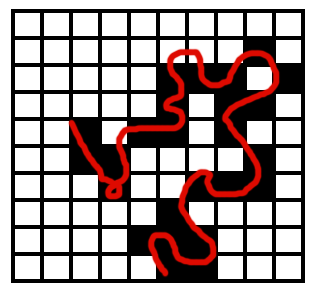
\includegraphics[width=.5\mycolumnwidth]{Tipos_datos/Imprecision_raster.png}
\caption{\small Imprecisi�n de forma en el modelo de representaci�n r�ster. La divisi�n del espacio en unidades cuadradas impide la representaci�n fiel de entidades tales como curvas como la mostrada en trazo rojo en la figura.}
\label{Fig:Imprecision_raster} 
\end{figure}

El per�metro de una entidad geogr�fica estar� compuesto por l�neas horizontales o verticales exclusivamente y, adem�s, su longitud y la superficie que encierra ser�n respectivamente m�ltiplos del tama�o de celda y el �rea de dicha celda. Esta es la principal raz�n por la cual, si el uso principal que se le va a dar a una capa es su representaci�n gr�fica, deba optarse por el modelo vectorial. En caso contrario, y salvo que la resoluci�n sea suficientemente alta, los mapas creados mostraran la falta de resoluci�n y podr�n distinguirse las unidades m�nimas de la capas r�ster (al igual que pasa en una imagen digital \emph{pixelada}), teniendo un aspecto que no es el propio de un mapa, tal y como estamos acostumbrados a usarlo.

El hecho de que dentro de una celda el valor de la variable recogida sea constante, da lugar a ambig�edades como la mostrada en la figura \ref{Fig:Ambiguedad_raster}, donde una celda est� ocupada por dos valores distintos, pero solo puede asign�rsele uno de ellos, debiendo establecerse alg�n criterio sistem�tico para llevar esto a cabo.

Un hecho similar sucede en el ejemplo de la capa de v�as. Algunas celdas son atravesadas por m�s de una v�a, pero esa informaci�n se pierde, ya que el tama�o de celda no es suficiente para recogerla. La celda en cuesti�n aparece como celda de v�a, pero no sabemos cu�ntas diferentes la atraviesan, ni tampoco si entre ellas est�n enlazadas o no.

\begin{figure}[!hbt]   
\centering
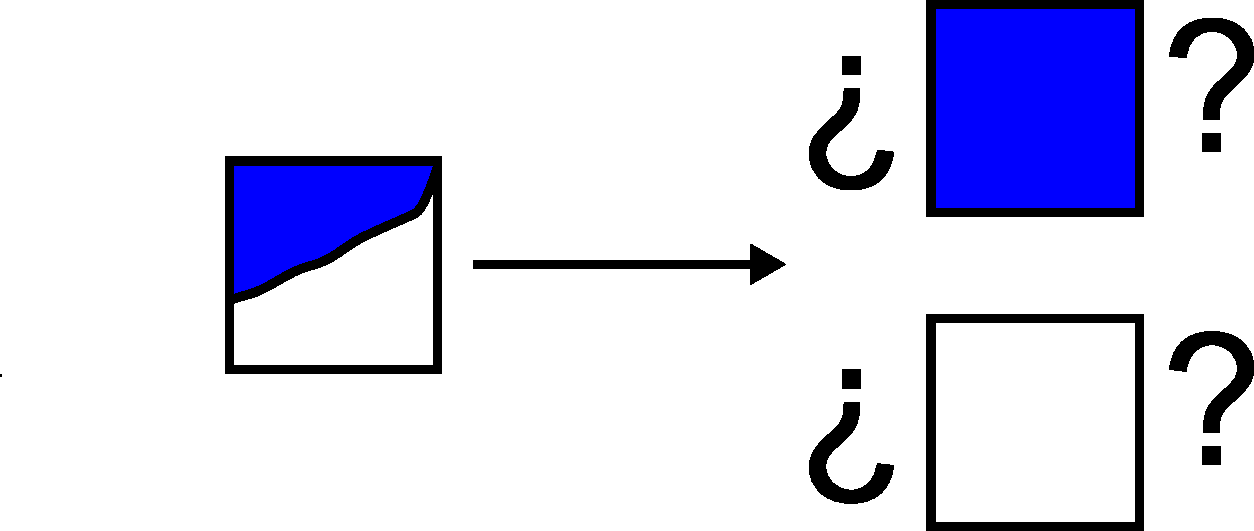
\includegraphics[width=.4\mycolumnwidth]{Tipos_datos/Ambiguedad_raster.pdf}
\caption{\small Ambig�edad en la asignaci�n de valores a una celda en una capa r�ster, debido al tama�o de esta, que condiciona la precisi�n con la que puede recogerse la realidad existente sobre el terreno.}
\label{Fig:Ambiguedad_raster} 
\end{figure}

Hay que tener en cuenta, no obstante, que la precisi�n de la representaci�n vectorial es, precisamente, de la representaci�n como tal, es decir, del modelo, pero no del dato en s� que tenemos en dicho formato vectorial, el cual depende de otros condicionantes tales como la escala de trabajo. Existe siempre incertidumbre en los datos, y el modelo de almacenamiento no excluye esta circunstancia. Los aspectos relativos a la calidad de los datos, tanto para datos r�ster como vectoriales, se desarrollan en profundidad en el cap�tulo \ref{Calidad_datos}.
\item \textbf{Volumen de almacenamiento}. El n�mero de elementos a almacenar es, en general, muy superior en el caso del modelo r�ster. Esto es as� debido a que toda la superficie a recoger se divide en las mismas unidades, independientemente de la complejidad de la variable en cada punto o de la necesidad de estudiarla con mayor o menor detalle en unos puntos que en otros. Para variables que se conciban mejor seg�n un modelo conceptual de entidades discretas, el modelo vectorial resulta m�s adecuado, ya que todas las zonas sin entidades no es necesario registrarlas de modo explicito, mientras que en el modelo r�ster estas deben registrarse de igual modo que aquellas en las que s� existe informaci�n relevante.
Los modelos de almacenamiento r�ster que veremos en el siguiente punto solucionan en parte el problema de los grandes vol�menes de datos del modelo r�ster, y son un elemento importante en la implementaci�n eficiente del mismo.
\item \textbf{Complejidad}. La regularidad y sistematicidad de las mallas r�ster hacen sencillo el implementar algoritmos de an�lisis, muy especialmente aquellos que implican el uso combinado de varias capas. Cuando estas capas est�n en formato r�ster y existe coincidencia entre sus mallas de celdas, el an�lisis conjunto de estas resulta inmediato. Por el contrario, la irregularidad espacial de las capas vectoriales hace que la implementaci�n de los mismos algoritmos sea sumamente m�s compleja si se trabaja con estas capas.

La sencillez de las capas r�ster, tanto en su concepto como en su implementaci�n, se ve apoyada adem�s por el hecho de que una capa r�ster se puede asemejar a una matriz, y por tanto aplicar sobre ella una serie de herramientas y elementos matem�ticos en muchos casos bien conocidos y de f�cil comprensi�n.

Existe de igual forma una distinta complejidad en t�rminos de proceso y c�lculo. Los algoritmos sobre una base r�ster pueden ser costosos en t�rminos de tiempo por la necesidad de aplicarlos sobre un n�mero muy elevado de celdas y un gran volumen de datos (v�ase el punto anterior). Por el contrario, los algoritmos sobre una base vectorial son costosos debido a que las operaciones matem�ticas que implican son m�s complejas y requieren mayores n�mero de c�lculos (aunque los vol�menes manejados puedan tambi�n ser notables).
\end{itemize}

Mas all� de las anteriores diferencias, a la hora de planificar un trabajo dentro de un SIG y elegir los datos que emplearemos y el modelo de representaci�n ideal, lo importante es entender que no existe un modelo de representaci�n id�neo de forma global, sino que esta idoneidad depende de muchos factores, como por ejemplo:

\begin{itemize}
 \item \textbf{Tipo de variable o fen�meno a recoger}. Como ya sabemos, algunas variables, en funci�n de su variabilidad y comportamiento espacial, son m�s adecuadas para el modelo vectorial, mientras que otras lo son para el modelo r�ster. Por ejemplo, en el caso de variables que requieran una intensidad de muestreo distinta seg�n la localizaci�n (variables que resulta interesante estudiar con m�s detalle en unos puntos que en otros) puede resultar m�s l�gico recogerlas de forma vectorial, pues el modelo r�ster implica una intensidad de muestreo constante a lo largo del �rea estudiada.
\item \textbf{Tipo de an�lisis o tarea a realizar sobre dicha variable}. El uso que demos a una capa tem�tica condiciona en gran medida el modelo de datos id�neo. Por ejemplo en el caso de una capa de elevaciones, su an�lisis se lleva mejor a cabo si esta informaci�n est� recogida seg�n el modelo r�ster. Sin embargo, si el objetivo principal es la visualizaci�n de esa elevaci�n en conjunto con otras variables, unas curvas de nivel pueden resultar m�s adecuadas, ya que, entre otras cosas, no interfieren tanto con otros elementos a la hora de dise�ar un mapa con todas esas variables.
\item \textbf{Contexto de trabajo}. Por ejemplo, si queremos trabajar con im�genes, esto nos condiciona al empleo de datos r�ster, ya que resulta mucho m�s sencillo combinarlos con las im�genes, las cuales siempre se presentan como capas r�ster. 
\end{itemize}

As�, en el desarrollo de un trabajo pueden aparecer circunstancias que hagan m�s adecuado utilizar el modelo r�ster y otras en las que el modelo vectorial sea m�s id�neo. En tal caso, deben combinarse ambas, pues es de esta forma como se obtendr�n mejores resultados. Un usuario de SIG no debe limitarse a trabajar de forma general con un �nico modelo de datos, con independencia del tipo de tarea que desempe�e, pues en cualquier caso ambos modelos de datos pueden aportar alguna ventaja.

Por �ltimo, es importante tener en cuenta que existen procedimientos para convertir entre los formatos r�ster y vectorial, de forma que el disponer de datos en un modelo de representaci�n particular no implica que debamos desarrollar nuestro trabajo sobre dichos datos directamente, sino que podemos efectuar previamente una conversi�n. Los cap�tulos \ref{Creacion_capas_raster} y \ref{Creacion_capas_vectoriales} tratan estos temas en profundidad.

\section{Modelos de almacenamiento}
\label{Modelos_almacenamiento}

\index{Modelo!de almacenamiento}
Los modelos de almacenamiento son el ultimo escal�n en la cadena de etapas distintas que llevan desde la realidad existente al conjunto de simples valores num�ricos que almacenamos y manejamos en un SIG y que modelizan dicha realidad. Los modelos de representaci�n definen una forma de recoger la realidad mediante unidades b�sicas (sean estas celdas en una malla, o bien primitivas geom�tricas definidas de una u otra manera), mientras que los modelos de almacenamiento plantean b�sicamente un esquema de c�mo convertir dichas unidades en valores num�ricos de la forma m�s eficiente. Es decir, c�mo \emph{escribir} dichos valores en un soporte digital o guardarlos en la memoria del ordenador de la mejor manera posible.

Los modelos de almacenamiento deben atender principalmente a dos necesidades b�sicas, que son las que definir�n su idoneidad para cada tarea y tipo de dato:

\begin{itemize}
 \item Minimizar el espacio ocupado por los datos.
\item Maximizar la eficiencia de c�lculo.
\end{itemize}

La primera necesidad es especialmente importante, pues, como ya se ha dicho, los datos r�ster son con frecuencia muy voluminosos. Un modelo de representaci�n que minimice el tama�o de los datos, unido a un manejo �ptimo de memoria, son requisitos de suma importancia para todo SIG que maneje datos r�ster, m�xime considerando los grandes vol�menes de datos que hoy en d�a se manejan, tales como los correspondientes a im�genes de alta resoluci�n.

La necesidad de maximizar la eficiencia de c�lculo afecta principalmente a las representaciones vectoriales ya que en ellas las operaciones son complejas. La forma en que se estructuran los valores de cada entidad ha de minimizar el numero de accesos necesarios a estos, para de este modo obtener un mejor rendimiento en todas las operaciones de an�lisis.

\subsection{Modelos para representaciones r�ster}

El principal problema relativo al almacenamiento de capas r�ster se presenta para el conjunto de valores de las distintas celdas, que constituye la parte m�s voluminosa de la informaci�n recogida. Las coordenadas de las celdas de referencia o el tama�o de celda, por su escaso volumen, no conllevan dificultad alguna, y es en el almacenamiento de la malla de celdas en s� donde se encuentran las diferencias entre unos y otros modelos.

La forma m�s inmediata de almacenar una capa r�ster es simplemente almacenar sus valores uno a uno, en una estructura similar a la que la propia capa representa. Para el caso m�s habitual de capas con celdas cuadradas, sabemos que la malla de datos correspondiente se puede asimilar a una matriz, con las implicaciones que esto tiene a la hora de su manejo. As�, la forma m�s directa de recoger una malla de datos r�ster es mediante una matriz de datos. Esta forma de almacenamiento tiene las siguiente ventajas \cite{Egenhofer1991Maguire}:

\index{Matriz!de datos (modelo almacenamiento)}

\begin{itemize}
 \item \textbf{Formato muy intuitivo}. La mayor�a de desarrolladores est� familiarizado con el concepto de matriz y con las operaciones de calculo matricial que pueden aplicarse sobre estas.
\item \textbf{Sencillez en la implementaci�n}. Los lenguajes de programaci�n soportan sin problemas el uso de matrices bidimensionales y una serie de operaciones b�sicas sobre ellas.
\item \textbf{Estructura}. Las mismas operaciones pueden aplicarse sobre todos los valores de la matriz de igual modo (todas las posiciones de la matriz son \emph{iguales} desde este punto de vista), lo que simplifica la implementaci�n de operaciones.
\item \textbf{Iterabilidad}. Resulta igualmente sencillo recorrer la matriz e iterar sobre la misma, lo cual refuerza lo anterior y simplifica a�n m�s la implementaci�n de todo tipo de procesos.
\end{itemize}

No obstante, el almacenamiento de todos los valores de forma id�ntica ignora el hecho de que pueden existir valores similares en zonas concretas, que pueden recogerse de formas mucho m�s �ptimas que una serie de n�meros iguales. En otras palabras, y de modo similar a como ocurre con el propio modelo de representaci�n r�ster, la estructura regular que confiere las ventajas es tambi�n la responsable de la mayor parte de los inconvenientes.

Como veremos en el cap�tulo \ref{Analisis_espacial}, las zonas pr�ximas entre s� (es decir, en el caso de una capa r�ster, las celdas pr�ximas entre s�), tienden a tener valores similares, en lo que se conoce como \emph{autocorrelaci�n espacial}. No considerar este hecho lleva al almacenamiento de informaci�n redundante, y ese es precisamente el principal problema del almacenamiento directo de una capa r�ster mediante una matriz. Almacenando expl�citamente todos los valores de la malla se desperdicia en muchos casos una gran cantidad de espacio (sea este en memoria, disco u otro soporte cualquiera).\index{Autocorrelaci�n espacial}

Podemos ver dos ejemplos claros de esto en las figuras \ref{Fig:Vias_modelos_representacion} y \ref{Fig:Malla_raster_rotada}. En la primera, existen �nicamente dos valores: los correspondientes a las celdas sobre las que se sit�a una v�a, o los correspondientes a las celdas donde estas no aparecen. Estos �ltimos ocupan la gran mayor parte de la capa, y lo hacen en bloque, de tal forma que almacen�ndolos individualmente se acaba teniendo una matriz de datos donde la practica totalidad de ellos son id�nticos. Como es f�cil de entender, este forma de proceder no es la m�s adecuada, al menos en t�rminos de volumen de almacenamiento.

En la segunda imagen, las zonas que aparecen como consecuencia de la rotaci�n de la imagen no contienen datos (esto es, contendr�n el valor arbitrario que codifica la falta de datos). Estas zonas tambi�n constituyen grandes bloques de celdas contiguas, con lo que el almacenamiento de todos los valores tambi�n es una soluci�n altamente redundante, especialmente en estas zonas fuera de la imagen como tal.

La soluci�n m�s habitual para considerar la redundancia de valores y lograr una compresi�n eficaz de los datos es la t�cnica denominada \emph{Run--Length Encoding}. \index{Run--Length Encoding}Esta t�cnica sencilla codifica una serie de $n$ valores id�nticos como un par de valores, el primero de los cuales representa el valor dicho que se repite $n$ veces, y el segundo es el n�mero de veces que se repite, esto es, $n$. 

As�, si la primera fila de la capa de v�as en formato r�ster no aparece ninguna celda de v�a, todas las celdas de dicha fila contendr�n el valor con que se codifica la ausencia de estas (sea, por ejemplo, el valor 0). El almacenamiento directo de todos los valores de la fila requerir�a tantos valores como columnas existan (sea $n$ el ancho de la fila), mientras que utilizando \emph{Run--Length Encoding}, bastar�a con almacenar el par (0, $n$).

A la hora de tratar el conjunto de todas las celdas, se define un orden en el que recorrerla, denominado \emph{orden de barrido} o \emph{de escaneo} (Figura \ref{Fig:Orden_escaneo}), de tal modo que la matriz bidimensional queda reducida a una cadena de valores, es decir, a un vector unidimensional. Los distintos \emph{trozos} de esa cadena se van codificando seg�n el esquema anterior, de tal modo que cuando aparecen muchos valores iguales consecutivos, estos pueden sustituirse ventajosamente por un �nico par de valores.\index{Orden!de barrido}\index{Orden!de escaneo}

\begin{figure}[!hbt]   
\centering
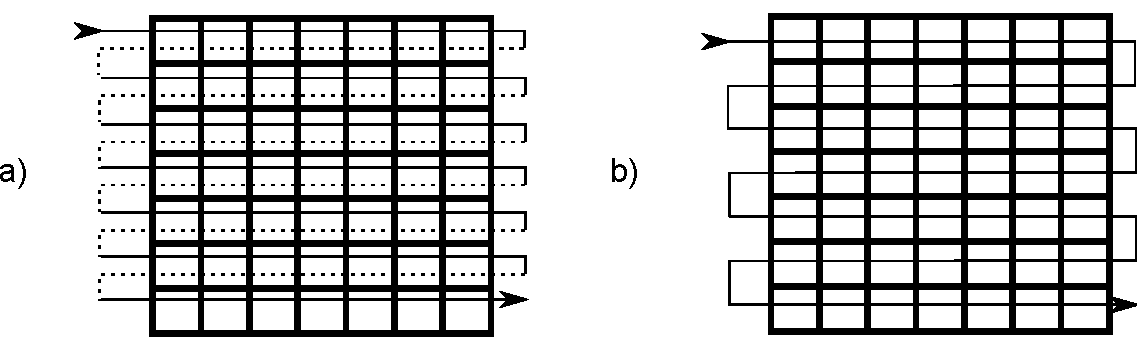
\includegraphics[width=.75\mycolumnwidth]{Tipos_datos/Ordenes_escaneo.pdf}
\caption{\small Ordenes de escaneo. a) fila a fila sin retorno, b) fila a fila con retorno.}
\label{Fig:Orden_escaneo} 
\end{figure}
 
La forma m�s sencilla de recorrer la imagen es hacerlo por filas, empezando por la fila superior y desplaz�ndose de derecha a izquierda (Figura \ref{Fig:Orden_escaneo}a). No obstante, el salto que se produce al final de cada fila suele implicar una discontinuidad en los valores. Invirtiendo la direcci�n del recorrido en cada fila, se tiene el orden mostrado en la figura \ref{Fig:Orden_escaneo}b, el cual suele tener como resultado mayores niveles de compresi�n de datos, ya que la cadena resultante de recorrer la imagen contiene \emph{trozos} generalmente de mayor tama�o.

Un esquema de barrido m�s complejo es el basado en el denominado \emph{orden de Morton} \cite{Morton1966IBM}. El orden de Morton (tambi�n conocido como \emph{orden Z}), se basa en una curva de car�cter recursivo, que recorre las celdas de la matriz siguiendo tramos en forma de Z, de ah� el nombre. En la primera iteraci�n se divide el conjunto de celdas en cuatro bloques, los cuales se recorren siguiendo el antedicho recorrido en Z. Si los bloques contienen a su vez m�s de una celda, se siguen subdividiendo a su vez de forma id�ntica, y as� hasta que no pueda continuarse este proceso.\index{Orden!Z}

La matriz que contiene los valores de orden de Morton (el orden en que se visita cada celda seg�n el esquema anterior), se conoce como \emph{Matriz de Morton}, la cual ya citamos por su importancia hist�rica en el cap�tulo \ref{Historia}.\index{Matriz!de Morton}\index{Orden!de Morton}\index{Morton!matriz de}\index{Morton!orden de}

\begin{figure}[!hbt]   
\centering
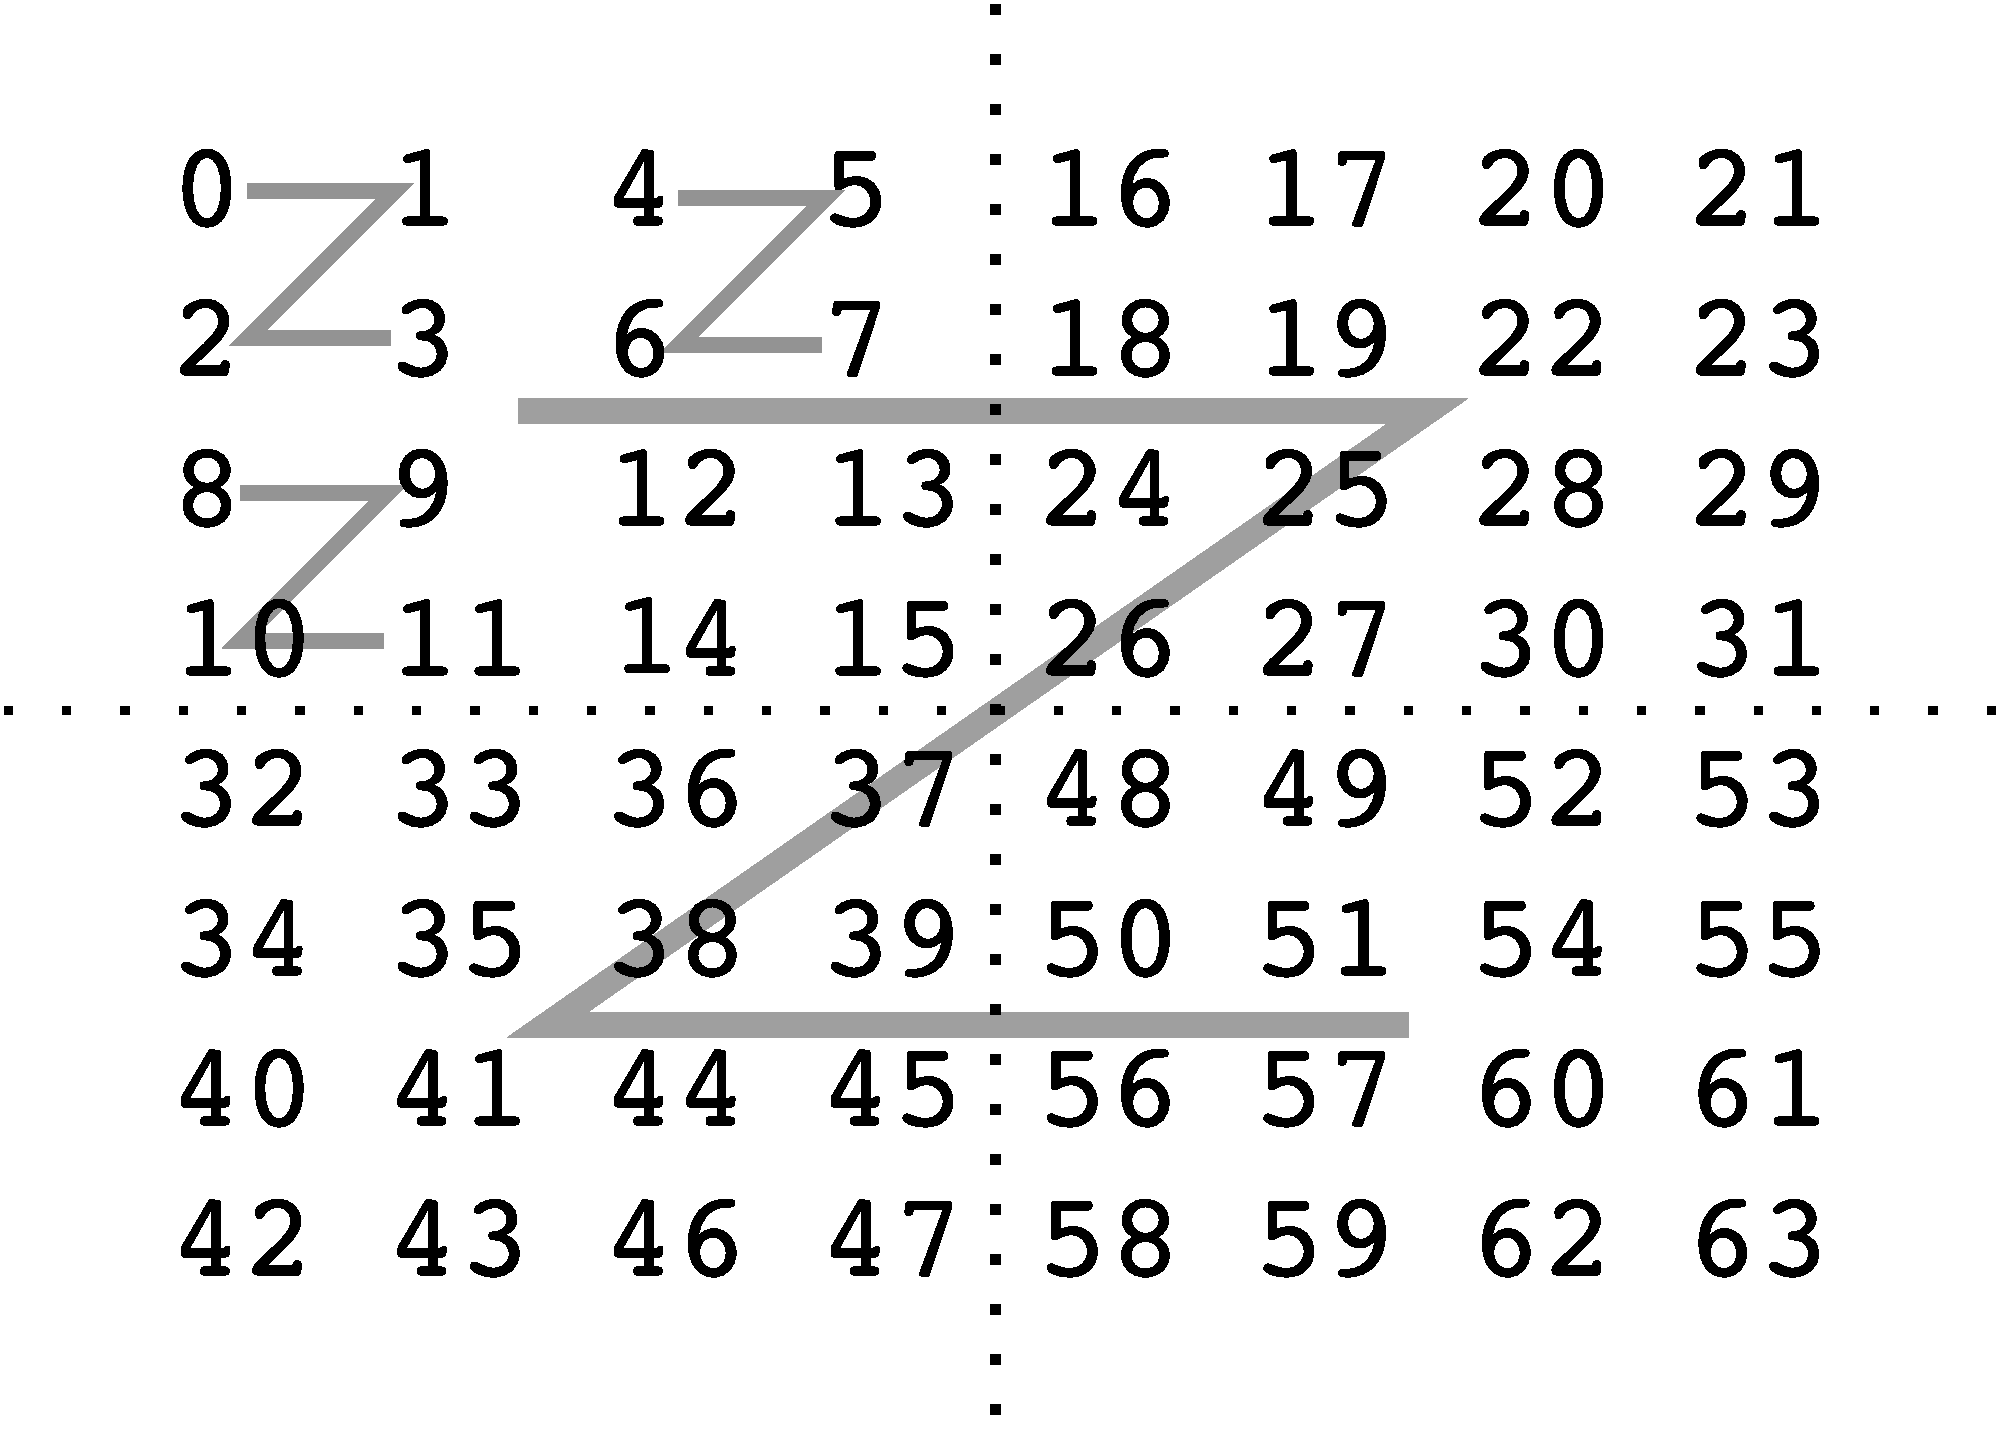
\includegraphics[width=.4\mycolumnwidth]{Tipos_datos/Orden_Morton.pdf}
\caption{\small Un ejemplo sencillo de barrido de una capa r�ster seg�n �rdenes de Morton. Los valores en las celdas no indican los valores de la variable, sino el orden en que se visita dicha celda seg�n este esquema de barrido}
\label{Fig:Orden_Morton} 
\end{figure}

Un ejemplo de este orden de barrido aplicado a una peque�a matriz puede verse en la figura \ref{Fig:Orden_Morton}.

Una estructura m�s avanzada son los denominados \emph{Quadtrees} o �rboles cuaternarios. Estas estructuras tambi�n dividen el espacio en cuadrantes sucesivamente, pero lo hacen con m�s profundidad en aquellas zonas que as� lo requieran por contener mayor n�mero de elementos y necesitar mayor resoluci�n. En el caso de una capa r�ster, se requerir� m�s detalle siempre que todas las celdas dentro de un cuadrante no tengan el mismo valor. En el caso m�s extremo, se ha de descender hasta el nivel de una sola celda, pero puede ser que un bloque de celdas contiguas tenga el mismo valor, en cuyo caso el cuadrante correspondiente las engloba a todas y las define con dicho �nico valor, sin necesidad de subdividirse m�s. De este modo, se adapta el modelo de almacenamiento a la propia estructura de la capa y al comportamiento que en esta muestra la variable estudiada.
\index{Quadtree}

Un ejemplo gr�fico de un �rbol cuaternario puede encontrarse en la figura \ref{Fig:Quadtree}. Los arboles cuaternarios son empleados tambi�n en los \emph{�ndices espaciales}, asociados a representaciones vectoriales, que veremos en \ref{Indices_espaciales} (de hecho, puede apreciarse que la figura anterior representa la aplicaci�n de un �rbol cuaternario a un conjunto de puntos, no a una capa r�ster, aunque el concepto es el mismo y su aplicaci�n a este segundo caso se realiza como ya se ha mencionado previamente).

Los quadtrees son estructuras complejas, y no profundizaremos m�s en su descripci�n dentro de este cap�tulo. Para el lector interesado, la definici�n original de esta estructura de datos puede encontrarse en \cite{Finkel1974Acta}. 

\begin{figure}[!hbt]   
\centering
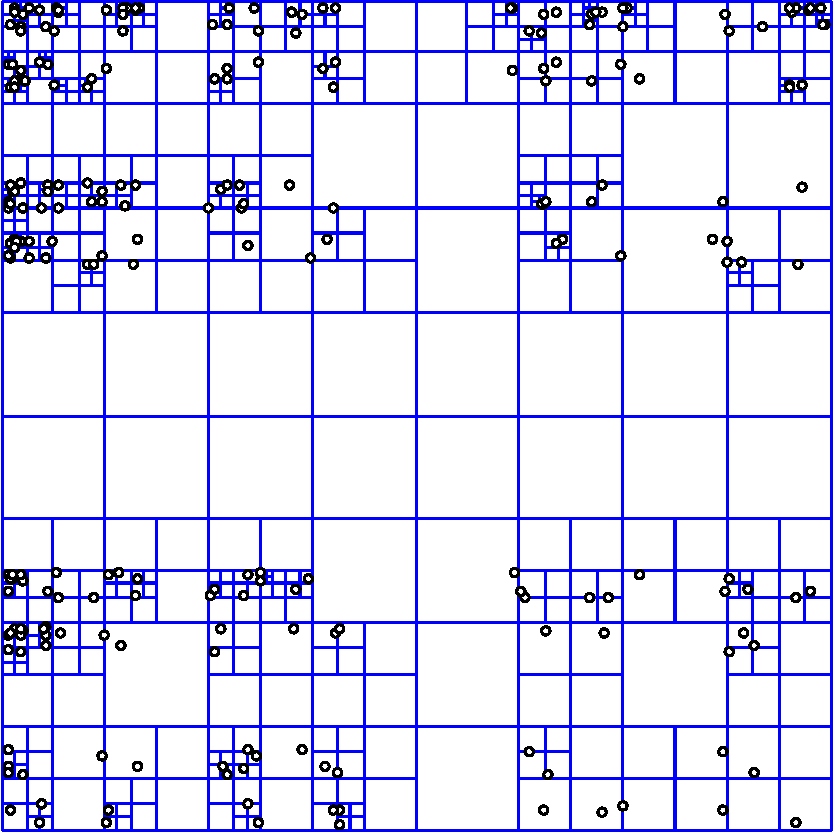
\includegraphics[width=.4\mycolumnwidth]{Tipos_datos/Quadtree.pdf}
\caption{\small Ejemplo de un �rbol cuaternario. En las zonas con m�s variabilidad (mayor densidad de puntos), los cuadrantes se subdividen hasta una profundidad mayor. La estructura es tal que cada cuadrante tiene dentro a lo sumo un punto. (Tomado de Wikipedia)}
\label{Fig:Quadtree} 
\end{figure}

Es importante rese�ar que cuando la capa r�ster contiene una informaci�n tal como una red viaria, la cual es susceptible de presentar valores id�nticos en celdas contiguas, la codificaci�n de tipo \emph{Run--Length} ---con cualquiera de los esquemas de barrido anteriores--- es ventajosa. Sin embargo, no lo es tanto cuando se trabaja con otro tipo de variables. 

En una capa con valores de elevaci�n, las celdas pr�ximas tendr�n valores parecidos pero no id�nticos, con lo que no podr� sacarse partido a esta forma de almacenamiento. M�s a�n, en estos casos el volumen ocupado por los datos no solo no disminuye, sino que aumenta. Es por ello que los SIG han de implementar igualmente la capacidad de poder trabajar con uno u otro modelo de almacenamiento seg�n los casos, bien sea por elecci�n directa del usuario o tom�ndose de forma autom�tica el que el propio sistema considere m�s adecuado en cada ocasi�n.

Aunque el mayor problema de las capas r�ster es su gran volumen, tambi�n existen diversas alternativas enfocadas a mejorar la velocidad de acceso a datos y el rendimiento de las operaciones sobre estas capas. Estas alternativas afectan a las im�genes con m�ltiples bandas, ya que estas, como dijimos, se recogen en un �nico fichero, en el cual se incorpora toda la informaci�n de las distintas bandas.\index{Bandas}

La forma en la que las bandas se tratan dentro del fichero y el modo en que se ordenan los p�xeles de las distintas bandas, ambas definen el esquema de almacenamiento, presentando cada uno de ellos una serie de ventajas de rendimiento en funci�n de la actividad principal que se vaya a desarrollar con la imagen. Tres son los esquemas principales:

\index{Band Sequential (BSQ)}
\index{Band Interleaved by Lines (BIL)}
\index{Band Interleaved by Pixel (BIP)}
\index{Pixel}

\begin{itemize}
	\item \emph{Band Sequential} (BSQ). Los valores se almacenan por bandas. Es decir, primero todos los p�xeles de la banda 1, despu�s los de la banda 2, y as� sucesivamente. Este tipo de esquema da prioridad a la componente espacial, ya que permite acceder r�pidamente a todo el espacio cubierto por una banda, puesto que los p�xeles de dicha banda se encuentran almacenados en posiciones contiguas.
	\item \emph{Band Interleaved by Pixel} (BIP). Los valores se almacenan ordenados por posiciones de p�xel. Es decir, primero se almacenan todos los valores correspondientes al p�xel (0, 0)\footnote{Es una terminolog�a habitual empezar a contar en cero en lugar de en uno las coordenadas fila/columna de una imagen} (en todas las bandas existentes), despu�s los correspondientes al (0,1)\footnote{Es habitual recorrer la imagen por filas, de forma que la coordenada (0,1) representa la primera fila y la segunda columna}, y as� sucesivamente.
	En caso de que lo que interese sea, para un p�xel dado, conocer toda la informaci�n disponible (su valor en todas las bandas), el esquema BIP es m�s ventajoso, ya que permite accesos r�pidos a este tipo de informaci�n, sin necesidad de <<saltar>> de un valor a otro como suceder�a en el caso del esquema BSQ. A nivel de acceso, se prima la informaci�n espectral sobre la espacial.
	\item \emph{Band Interleaved by Lines} (BIL). Es un esquema intermedio en el que se recogen los valores por filas. Esto es, primero la fila 1 de la banda 1, luego la de la banda 2, y as� sucesivamente. Posteriormente se recoge la fila 2 para todas las bandas, y de este modo hasta cubrir toda la imagen. Se trata de un esquema intermedio entre los anteriores, permitiendo un acceso r�pido tanto a la informaci�n espacial como a la informaci�n espectral de las bandas.
\end{itemize}

La figura \ref{Fig:Esquemas_almacenamiento_bandas} se muestra un ejemplo muy sencillo de los anteriores esquemas. Para una imagen de $2\times 2$ celdas y dos bandas, se recoge el orden en que se almacenar�a capa valor seg�n cada uno de dichos esquemas.

\begin{figure}[!hbt]   
\centering
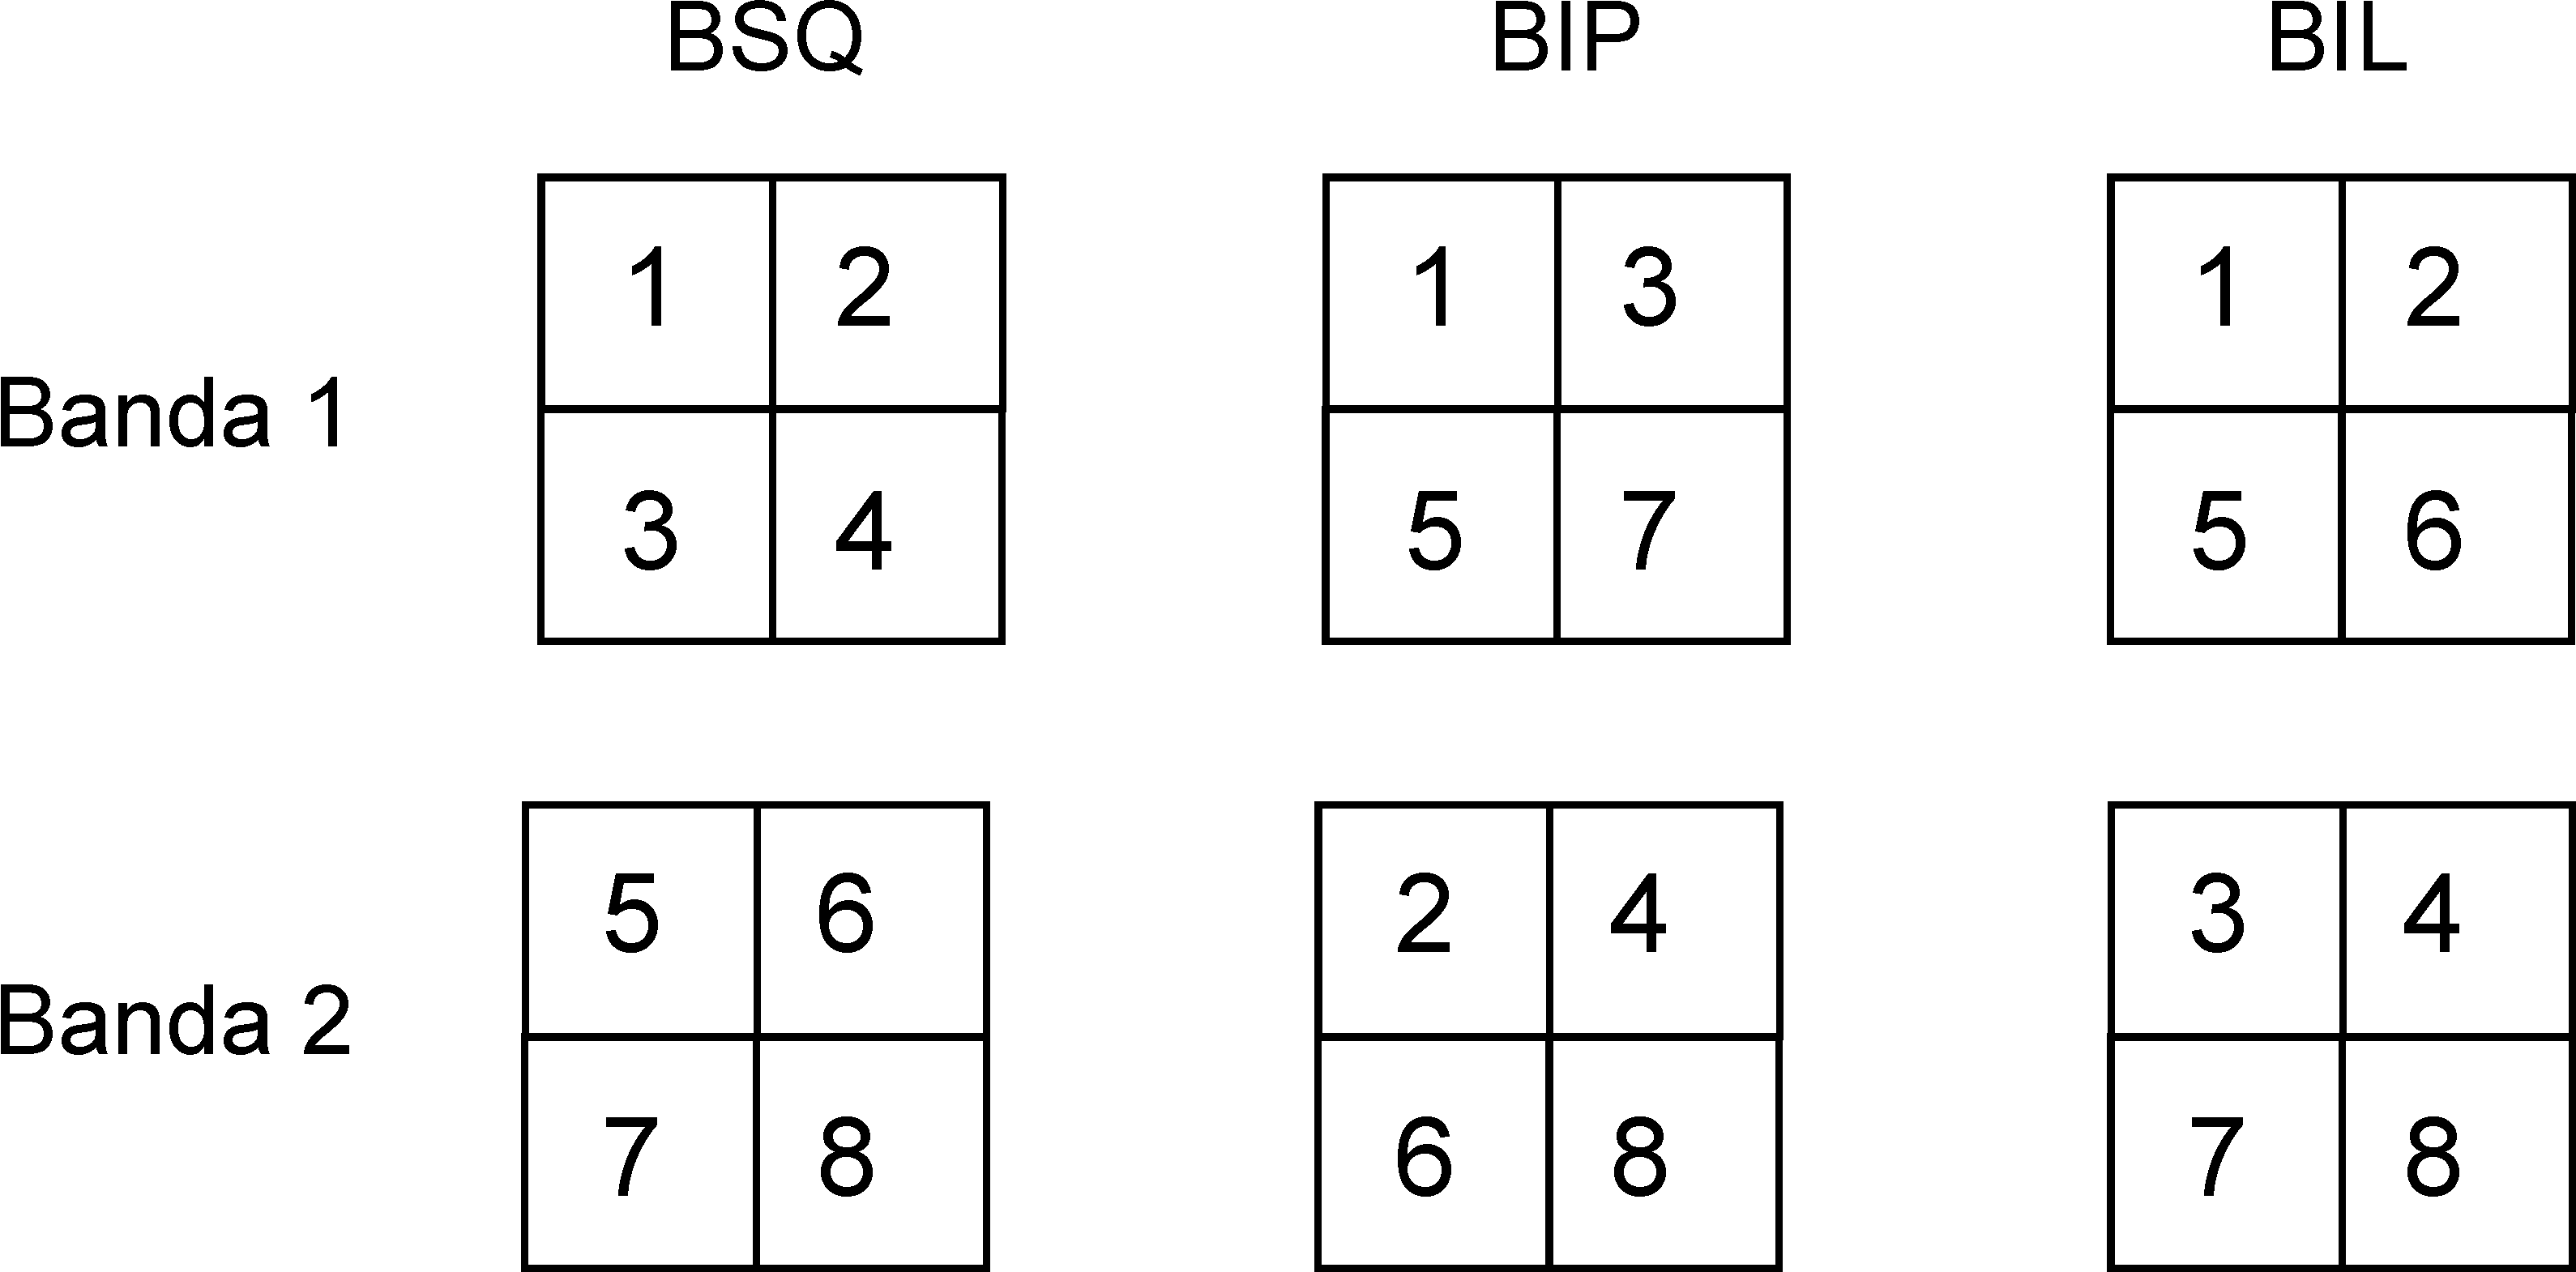
\includegraphics[width=.5\mycolumnwidth]{Tipos_datos/Esquemas_almacenamiento_bandas.pdf}
\caption{\small Esquemas de almacenamiento para im�genes multibanda. Los n�meros indican el orden en que se almacena cada valor.}
\label{Fig:Esquemas_almacenamiento_bandas} 
\end{figure}

\subsection{Modelos para representaciones vectoriales}

Al igual que para el modelo r�ster, existen para el modelos vectorial diferentes alternativas a la hora de almacenar los elementos que componen una capa. En realidad, ya hemos visto dentro de este cap�tulo algo que se asemeja a un modelo de almacenamiento, pues los modelo topol�gicos como DIME o el modelo \emph{arco--nodo}\index{Arco--nodo}, o los detallados para el caso particular de las redes, todos son en realidad esquemas de almacenamiento para el conjunto de \emph{piezas} que componen esa estructura topol�gica que se quiere almacenar. No obstante, tambi�n tienen algo de modelos de representaci�n, pues existe variaci�n en la forma en que conciben las partes de cada entidad (arcos entre dos nodos con o sin v�rtices intermedios, seg�n el modelo). 

En realidad, la raz�n por la que se han presentado en una secci�n anterior es porque de ese modo ayudaban a comprender mejor la existencia o no de topolog�a en una representaci�n, y ese aspecto resulta m�s importante para el estudio de los SIG que los modelos de almacenamiento. Estos, como se ha dicho, est�n a un nivel m�s bajo y alejado del usuario.

En general, los modelos de datos vectoriales no buscan tanto la disminuci�n de volumen de los datos como la obtenci�n de una mayor eficacia en las operaciones y una simplificaci�n de estas. L�gicamente, si los datos tienen un volumen menor, el tiempo que cualquier operaci�n sobre ellos implica tambi�n ser menor. A�n as�, la diferencia principal para este tipo de datos reside en la disminuci�n de la complejidad en que estos se almacenan, disminuyendo las operaciones a realizar, as� como la  complejidad de la implementaci�n de los correspondiente algoritmos (ambas habitualmente elevadas).

Para mejorar el rendimiento de las operaciones que trabajan con datos vectoriales, un factor clave es mejorar el acceso a los datos, de forma que, cuando se necesite acceder a unos datos concretos, estos puedan <<encontrarse>> de forma f�cil. Por este motivo, un elemento importante en la representaci�n de los datos vectoriales son los denominados \emph{�ndices espaciales}.\index{Indice@�ndice!espacial}

El concepto de �ndice cuando se habla de datos es similar al concepto de �ndice referido a un libro como este. Aqu� tienes un ejemplo muy sencillo para que lo comprendas mejor: si vas al principio de este libro, puedes ver su �ndice y saber d�nde empieza este cap�tulo, de forma que si estas interesado en modelos relacionados con la informaci�n geogr�fica, sabes r�pidamente que es en este bloque de p�ginas donde debes buscar lo que te interesa. Si no existiera ese �ndice, tendr�as que ir revisando todas las p�ginas hasta que llegaras al principio de cap�tulo y te dieras cuenta de que aqu� es donde est� lo que buscas. De igual modo, si vas al final de este libro y buscas el t�rmino \emph{�ndices espaciales}, ver�s que aparece esta p�gina junto con otras en las que aparece dicho t�rmino. Si no tuvieras ese �ndice, tendr�as que revisar palabra por palabra para saber en qu� partes de este libro se habla de �ndices espaciales.

Estos sencillos ejemplos muestran situaciones similares a las que aparecen en el uso habitual de un SIG, en las cuales trabajamos sobre una parte del total de los datos. Igual que buscamos un cap�tulo o un �nico t�rmino, podemos querer, por ejemplo, todas las entidades de una capa que est�n en una zona particular del espacio. Disponer de un �ndice acelera el proceso de localizar esas entidades que nos interesan. Por trabajar con informaci�n espacial, tales �ndices se denominan �ndices espaciales.

Muchos de los procesos que veremos en la parte dedicada al an�lisis necesitan este tipo de �ndices para poder ejecutarse con un rendimiento adecuado. A medida que veamos estos procesos, se comprender� mejor por qu� la existencia de �ndices espaciales resulta necesaria e incluso imprescindible cuando disponemos de datos de gran volumen. En el cap�tulo \ref{Consultas} veremos informaci�n m�s detallada sobre la utilidad de los �ndices espaciales, ya que estos son vitales para la realizaci�n de consultas espaciales, que son tratadas en dicho cap�tulo.\index{Consultas}

Como ya hemos dicho, el objetivo de este tipo de estructuras para representar los datos espaciales no es disminuir el tama�o, sino mejorar el rendimiento de las operaciones sobre ellos. De hecho, y al contrario que en el caso de los modelos de representaci�n r�ster, en este caso no disminuye el espacio que ocupan los datos, sino todo lo contrario, ya que este aumenta. Un �ndice espacial es informaci�n adicional que incrementa la utilidad de dichos datos. Exactamente del mismo modo que el �ndice de este libro, que no sustituye al texto que ahora mismo estas leyendo, sino que se a�ade a este y te ayuda a manejarte a trav�s de �l y sacarle m�s partido.

La creaci�n del �ndice espacial supone la creaci�n de una estructura espacial en la cual se contienen objetos m�s simples que las propias entidades geom�tricas, estructuradas a su vez de forma tambi�n m�s sencilla que recogiendo sus coordenadas, y con un orden caracter�stico. Como hemos dicho, este �ndice espacial no sustituye al dato espacial, sino que lo complementa, optimizando la b�squeda de informaci�n dentro de este.

Existen dos enfoques principales para los �ndices espaciales: continuos y discretos \cite{Guting1994VLDB}. Los continuos utilizan las coordenadas mismas de las entidades, simplificando la forma de estas, mientras que en los discretos la simplificaci�n se aplica al espacio, discretizando este. En ambos, las entidades que se emplean son rectangulares en la mayor�a de los casos. La figura \ref{Fig:Tipos_indices_espaciales} muestra la aproximaci�n de una geometr�a poligonal que se obtiene en ambos tipos de modelos. 
\index{Indice@�ndice!espacial!tipos}

\begin{figure}[!hbt]   
\centering
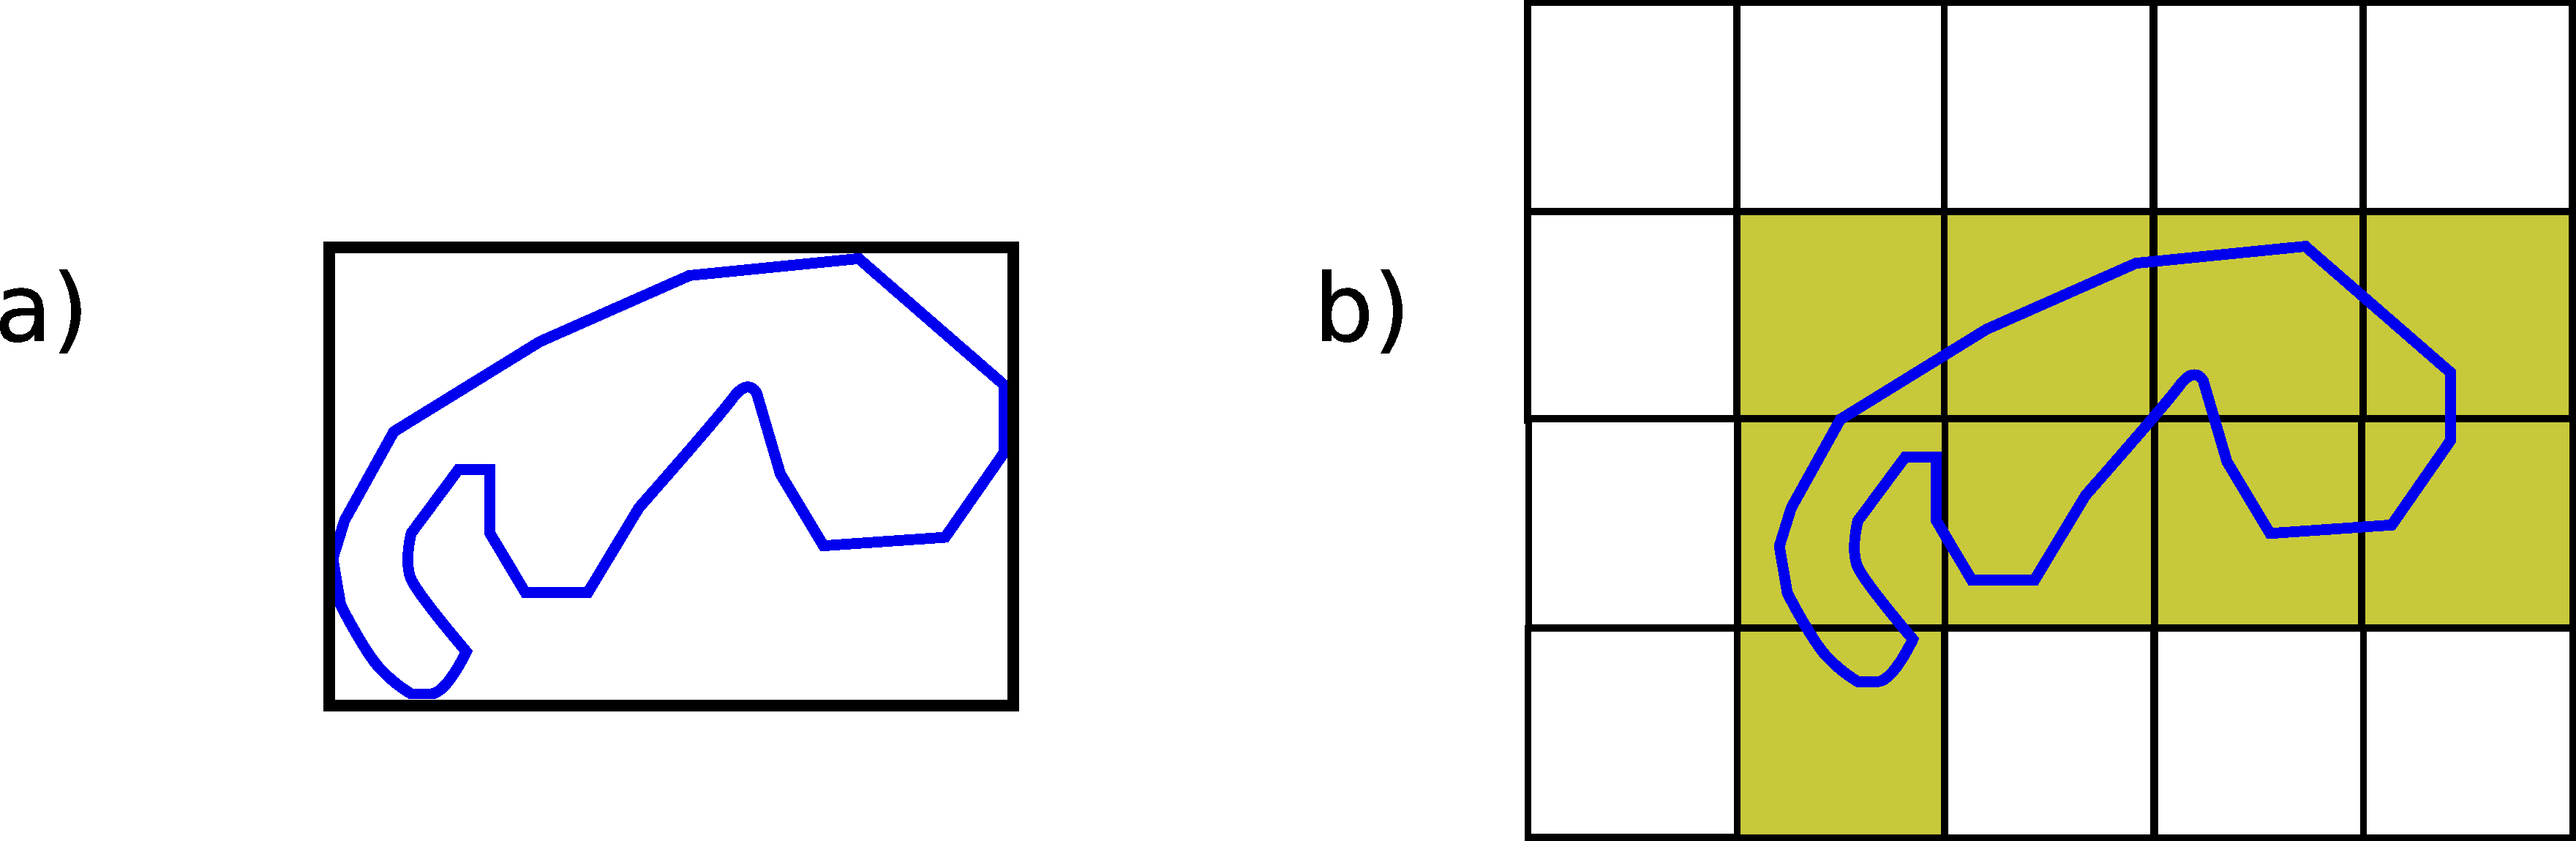
\includegraphics[width=.7\mycolumnwidth]{Tipos_datos/Tipos_indices_espaciales.pdf}
\caption{\small Aproximaci�n continua (a) y discreta (b) para un �ndice espacial.}
\label{Fig:Tipos_indices_espaciales} 
\end{figure}

En el caso continuo, se sustituye toda la complejidad del pol�gono por simplemente cuatro puntos: aquellos que conforman el rect�ngulo dentro del que este se inscribe. En el caso discreto, se reduce el pol�gono a unas cuantas celdas de una malla. Realizar comprobaciones sobre estas estructuras resulta mucho m�s sencillo, y por ello se emplean para realizar aproximaciones que simplifican las operaciones\footnote{Este proceso, conocido como \emph{filtrado y refinamiento}, lo veremos en detalle en el cap�tulo \ref{Consultas}}.\index{Filtrado y refinamiento}

Supongamos que utilizamos un �ndice espacial del primer tipo y queremos saber qu� pol�gonos de una capa se intersecan con otro dado. Para comprobar qu� pol�gonos se intersecan con este, en primer lugar podemos comprobar los solapes existentes entre sus rect�ngulos. Si los rect�ngulos no se solapan, es inmediato ver que los pol�gonos tampoco, con lo que no es necesario ya operar con ellos. Ver si dos rect�ngulos se solapan es casi inmediato, mientras que esta misma operaci�n para pol�gonos complejos requiere un numero mucho mayor de operaciones.

Debido al uso de rect�ngulos como elementos b�sicos, las estructuras que se emplean est�n espec�ficamente dise�adas para contener o bien rect�ngulos (en el caso de entidades de l�neas o de pol�gonos) o puntos (en el caso de entidades puntuales). Estas estructuras no son nuevas para nosotros, ya que hemos visto algunas de ellas en este mismo cap�tulo. Por ejemplo, para el caso de una aproximaci�n continua sobre una capa de puntos, los arboles cuaternarios (\emph{quadtrees}) son una estructura de datos adecuada. Esta aplicaci�n ya la vimos, de hecho, en la figura \ref{Fig:Quadtree}.

Como seguramente ya hayas advertido, los enfoques continuo y discreto se corresponden a primera vista con las ideas correspondientes a los modelos de datos r�ster y vectorial (aunque los �ndices espaciales de los que estamos hablando son para capas vectoriales). Es por ello que las estructuras que hemos visto para el almacenamiento de datos r�ster pueden utilizarse tambi�n para recoger las distintas celdas de un �ndice espacial discreto. As�, la divisi�n en celdas hace necesario un orden de escaneo\index{Orden!de escaneo}. El orden de Morton que ya conocemos se aplica en este caso, entre otros.\index{Orden!de Morton}

Una vez m�s, las estructuras de datos de todos estos �ndices espaciales suponen un elemento demasiado especifico para los contenidos de este libro, por lo que no se profundizar� en su teor�a. No obstante, estos son numerosos, ya que se trata de un �rea muy desarrollada. Referencias como \cite{Buchmann1990Springer} aportan descripciones m�s extensas para el lector interesado.

En caso de querer profundizar en los aspectos m�s t�cnicos de la representaci�n del dato geogr�fico en general, tanto en formato r�ster como vectorial, \cite{Worboys2004CRC} ofrece informaci�n muy extensa al respecto.

\section{Resumen}

El proceso de almacenar la realidad y reducirla a un conjunto de valores num�ricos manejables por un ordenador implica tres etapas fundamentales: creaci�n de un modelo conceptual, adopci�n de un modelo de representaci�n y codificaci�n del anterior seg�n un modelo de almacenamiento. Estos procesos dan lugar a la creaci�n de las denominada \emph{capas geogr�ficas}, unidades fundamentales de informaci�n dentro de un SIG.

Dos son los modelos conceptuales m�s importantes: campos y entidades discretas. Estos a su vez se identifican en l�neas generales con los dos principales modelos de representaci�n: r�ster y vectorial.

En el modelo r�ster el espacio se divide sistem�ticamente en unidades m�nimas denominadas celdas, habitualmente de forma cuadrada. En el modelo vectorial se almacenan las distintas entidades geogr�ficas a trav�s de las coordenadas de los puntos que las componen. El concepto de \emph{topolog�a} es importante en el modelo vectorial, y en funci�n de la forma en que se recojan las coordenadas de cada entidad, se almacenar� o no la informaci�n topol�gica. El modelo arco--nodo es el m�s habitual para representar la topolog�a.

La ultima etapa es la que conlleva el almacenamiento de los modelos de representaci�n, convirtiendo los elementos base de estos en valores num�ricos manejables por el ordenador. Cada modelo de representaci�n tiene sus particulares modelos de almacenamiento, los cuales tratan de maximizar el rendimiento de las operaciones realizadas sobre los datos espaciales, al tiempo que reducen el espacio que dichos datos ocupan.

\pagestyle{empty}
%
\chapter{Fuentes principales de datos espaciales}
\label{Fuentes_datos}




No hace tanto tiempo, toda la informaci�n que se manejaba dentro de un SIG ten�a su origen en un mapa en papel, el cual deb�a \emph{prepararse} para adaptarse a la naturaleza propia del SIG. El dato geogr�fico se obten�a a partir de la \textbf{digitalizaci�n} de cartograf�a, es decir, convertir los datos geogr�ficos en formato impreso en datos en formato digital que un SIG pudiera manejar. 

Un SIG implica una aplicaci�n inform�tica, y esta se alimenta en �ltima instancia exclusivamente de datos digitales. Los datos geogr�ficos digitales tienen una serie de ventajas frente a los anal�gicos (adem�s del mero hecho de que podemos incorporarlos a nuestro SIG), y suponen, como sucede en muchos otros campos, un salto cualitativo importante. Entre estas ventajas, que son a su vez comunes a otros �mbitos,  destacan la sencillez de actualizaci�n, la facilidad de distribuci�n (en especial con la aparici�n de Internet), el menor espacio f�sico necesario para su almacenamiento, la facilidad y precisi�n del an�lisis, y la facilidad de mantenimiento (el dato digital no se degrada, lo que se degrada es su soporte, pero es sencillo replicar el dato sin p�rdida de calidad)

Hoy en d�a las t�cnicas de adquisici�n de datos han evolucionado y permiten crear datos que pueden ser directamente integrados en un SIG. Distinguimos as� \textbf{fuentes de datos primarias} y \textbf{secundarias}. 

Las fuentes de datos primarias son aquellas cuyos datos podemos emplear en un SIG, ya que estos, en su forma original, ya son susceptibles de ser sometidos a las operaciones de manejo y an�lisis que incorporan los SIG. Por su parte, las fuentes de datos secundarias generan datos que no pueden emplearse en un SIG sin un proceso de adaptaci�n previo, siendo el dato derivado el que utilizamos en un SIG, no el original. 

En este cap�tulo, veremos las distintas fuentes de datos con las que podemos trabajar un en SIG.


\section{Teledetecci�n}\index{Teledetecci�n}

La primera fuente de datos que trataremos en este cap�tulo es la teledetecci�n. Entendemos por teledetecci�n el estudio y medida de las caracter�sticas de una serie de objetos (en nuestro caso elementos de la superficie terrestre) sin que exista contacto f�sico. Para ello, se miden las perturbaciones que el objeto provoca en su entorno, principalmente las de tipo electromagn�tico.

Un sistema de teledetecci�n cuenta con los siguientes elementos (Figura \ref{Fig:Elementos_teledeteccion}):

\begin{figure}[!hbt]   
\centering
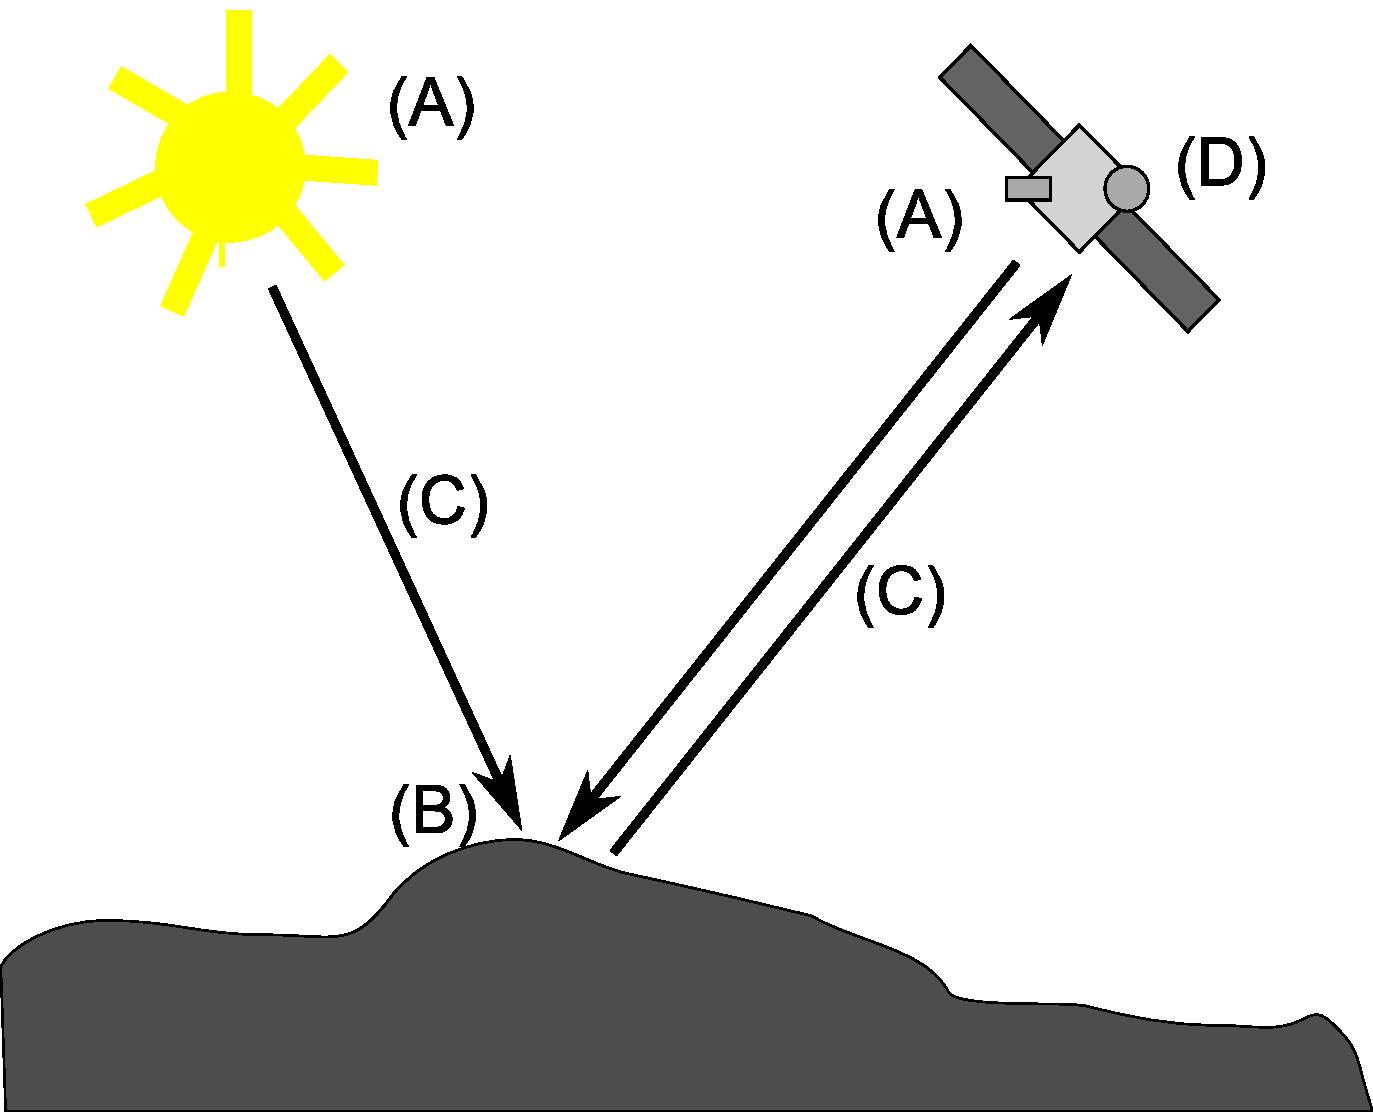
\includegraphics[width=.4\textwidth]{Fuentes_datos/Elementos_teledeteccion.pdf}
\caption{\small Esquema de un sistema de teledetecci�n.}
\label{Fig:Elementos_teledeteccion} 
\end{figure}


\begin{itemize}
	\item \textbf{Una fuente de radiaci�n (A)}\index{Fuente de radiaci�n}. Puede ser de origen natural o artificial. La radiaci�n emitida por dicha fuente llega al terreno y sufre una perturbaci�n causada por los elementos de este, siendo esta perturbaci�n el objeto de estudio de la teledetecci�n. Los propios objetos pueden ser tambi�n emisores ellos mismos de radiaci�n.
	\item \textbf{Unos objetos (B) que interaccionan con la radiaci�n} o la emiten, seg�n lo anterior.
	\item \textbf{Una atm�sfera (C)} por la que se desplaza la radiaci�n, tanto desde la fuente hasta el objeto como desde el objeto hasta el receptor. La atm�sfera tambi�n interact�a con la radiaci�n, introduciendo igualmente perturbaciones en ella.
	\item \textbf{Un receptor (D) que recoge la radiaci�n} una vez esta ha sido perturbada o emitida por los objetos. El receptor va a generar como producto final una imagen (en t�rminos de un SIG, una capa r�ster), en cuyas celdas o p�xeles se va a contener un valor que indica la intensidad de la radiaci�n. Estos valores son valores enteros que indican el nivel de dicha radiaci�n dentro de una escala definida (habitualmente valores entre 1 y 256), y se conocen dentro del �mbito de la teledetecci�n como \textbf{Niveles Digitales}.
\end{itemize}

A lo largo de este apartado veremos con detalle estos elementos. Para estudiar los dos primeros, estudiaremos los fundamentos f�sicos relativos a la radiaci�n y a la la interacci�n entre esta y la materia, mientras que para el estudio del sistema receptor analizaremos los elementos de este en dos componentes por separado: sensores y plataformas. 

La interacci�n de la atm�sfera interesa de cara a eliminar su efecto, ya que lo que resulta de inter�s en general son los objetos en la superficie terrestre, no la atm�sfera como tal. Eliminar esta influencia de la atm�sfera es parte de los procesos posteriores que se realizan con la imagen, y que se detallan en los cap�tulos dedicados al an�lisis de im�genes en lugar de en este.

\subsection{Fundamentos f�sicos}

La radiaci�n electromagn�tica es producto de las alteraciones en los campos el�ctrico y magn�tico, las cuales generan ondas correspondientes a cada uno de los campos magn�tico y el�ctrico. Estas ondas se desplazan a la velocidad de la luz, y se pueden describir con los par�metros habituales, tales como la longitud de onda o la frecuencia. El rango de longitudes de onda cubierta por la radiaci�n electromagn�tica se conoce como \textbf{espectro electromagn�tico}.

El espectro se subdivide en regiones en funci�n de su longitud de onda, tales como (de menor a mayor longitud de onda) los rayos $\gamma$, los rayos X, la regi�n ultravioleta, la regi�n visible, la regi�n infraroja, o las microondas  

La radiaci�n emitida por una fuente de radiaci�n es alterada por la presencia de los distintos objetos, ya que estos \textbf{absorben, transmiten} o \textbf{reflejan} esta.

Estos tres fen�menos se dan en diferente proporci�n en funci�n de las caracter�sticas del objeto y de la radiaci�n. La parte que  interesa a efectos de la teledetecci�n es aquella que se refleja en el objeto, ya que esta es la que posteriormente puede recogerse y emplearse para la generaci�n de las im�genes.

Como ya se dijo en el cap�tulo \ref{Introduccion_datos}, las im�genes como capas r�ster presentan habitualmente la particularidad de tener varias bandas. En lugar de un �nico valor para cada celda, existen $n$ valores, uno por cada banda. La imagen recoge la intensidad de la radiaci�n dentro de una amplitud dada del espectro, y a su vez subdivide esta en distintas franjas. Los Niveles Digitales de cada banda corresponden a la intensidad dentro de una de esas franjas del espectro en particular.

Puesto que cada objeto refleja la radiaci�n de diferentes longitudes de onda de modo distinto, esto puede considerarse como una propiedad del objeto. Se tiene as� el concepto de \textbf{firma espectral}, que es la respuesta caracter�stica de un tipo de objeto dentro del espectro electromagn�tico. 


\subsection{Sensores y plataformas}

En un sistema de teledetecci�n, dos son los elementos tecnol�gicos principales que lo definen: el \textbf{sensor} y la \textbf{plataforma}. 

El sensor es el elemento que incorpora la capacidad de <<leer>> la radiaci�n electromagn�tica y registrar su intensidad dentro de la una zona concreta del espectro. Puede ir desde una simple c�mara fotogr�fica hasta un sensor m�s especializado.

Los sensores se denominan \textbf{pasivos} aprovechan las fuentes de radiaci�n existentes en la naturaleza (fundamentalmente el Sol) y se limitan a recoger la radiaci�n de dichas fuentes reflejada por los elementos del medio, o \textbf{activos} s� emiten radiaci�n, y recogen dicha radiaci�n tras ser reflejada por dichos elementos. Para entender este concepto de un modo de un modo sencillo, podemos decir que una c�mara fotogr�fica es un sensor pasivo, mientras que una camara fotogr�fica con \emph{flash} es un sensor activo. La radiaci�n emitida por los sensores activos no ha de ser necesariamente luz visible (como en el caso del flash), sino que pueden emitir en otras secciones del espectro.

Tecnolog�as como el \textbf{radar} o el \textbf{LiDAR} (similar al radar pero con pulsos de laser en lugar de ondas de radio), se basan en sensores activos. En el caso del LiDAR, permite obtener imagenes que no tiene un caracter visual, sino que contienen en sus valores la elevaci�n de los objetos, pudiendo as� emplearse para cartografiar el relieve.


La plataforma, por su parte, es el medio en el que se sit�a el sensor y desde el cual se realiza la observaci�n.  A bordo de una plataforma pueden montarse varios sensores.

Los dos tipos principales de plataformas son aquellas situadas \textbf{{dentro de la atm�sfera} terrestre (aviones en su mayor�a) y aquellas situadas \textbf{fuera de la atm�sfera} (a bordo de sat�lites).

Los aviones tienen la ventaja de su \texbtf{disponibilidad}, ya que pueden pilotarse y de este modo permiten cubrir cualquier lugar de la tierra en cualquier momento.

A diferencia de un avi�n, un sat�lite no puede dirigirse a voluntad (no puede pilotarse), y su movimiento es una caracter�stica inherente que viene definida por una serie de par�metros. Estos par�metros se conocen como \textbf{{par�metros orbitales} pues definen la �rbita descrita por el sat�lite en torno a la Tierra. 

Las �rbitas pueden clasificarse en funci�n de su eje de rotaci�n as� como en funci�n de su movimientos. En este �ltimo caso tenemos �rbitas \textbf{geos�ncronas} (el sat�lite se sit�a sobre un punto fijo de la Tierra y su movimiento sigue al de rotaci�n de esta) o \textbf{helios�ncronas} (mientras el sat�lite recorre la �rbita, la Tierra efect�a su movimiento de rotaci�n, lo cual hace que a cada vuelta de la �rbita se cubran zonas distintas) 
	
	

\subsubsection{Resoluciones}

Uno de los par�metros principales que definen las propiedades de un sistema de teledetecci�n son las \emph{resoluciones}. Estas establecen el nivel de detalle de los productos que el sistema genera, determinando este en las distintas magnitudes en las que el sistema opera. Las resoluciones dependen del sensor y de la plataforma como binomio operativo, y de las caracter�sticas propias de ambos. Distinguimos cuatro resoluciones, a saber:

\begin{itemize}
	\item \textbf{Resoluci�n espacial}. Indica la dimensi�n del objeto m�s peque�o que puede distinguirse en la imagen. En l�neas generales es el equivalente al tama�o de p�xel\footnote{Desde un punto de vista formal, no ha de ser necesariamente as�, ya que la imagen puede tomarse originalmente con unas caracter�sticas y despu�s, mediante operaciones matem�ticas (veremos estas en el cap�tulo \ref{Algebra_de_mapas}), modificar el tama�o de p�xel\index{Pixel}. Aunque este tama�o sea menor al original, los objetos de menor dimensi�n que podr�n discernirse en esa imagen no ser�n iguales a ese tama�o, sino mayores.} es decir, a la dimensi�n real que un p�xel de la imagen tiene sobre el terreno.\index{Resoluci�n!espacial}
	
	La resoluci�n espacial est� en funci�n de la capacidad resolutiva del sensor y las caracter�sticas de la plataforma tales como la altura a la que se sit�a. Asimismo, la resoluci�n espacial esta relacionada con la superficie que cada imagen cubre sobre el terreno. El concepto de \emph{Campo Instant�neo de Visi�n}\footnote{Instantaneous Field of View (IFOV)} \index{Instantaneous Field of View (IFOV)} \index{Campo Instant�neo de Visi�n}indica el �ngulo de visi�n que abarca el sensor, y se utiliza habitualmente es este sentido. El \emph{Campo Instant�neo de Visi�n en Tierra}\footnote{Ground Instantaneous Field of Vision (GIFOV)}\index{Ground Instantaneous Field of Vision (GIFOV)} expresa esta misma idea pero en unidades de longitud sobre el terreno, y es funci�n del IFOV y la altura a la que se encuentre el sensor.\index{Campo Instant�neo de Visi�n en Tierra}
	
	En el dise�o de la �rbita de un sat�lite debe tenerse en cuenta el campo de visi�n del sensor para optimizar el ciclo de toma de im�genes, as� como para evitar que las distintas franjas que este cubre queden sin solaparse y existan zonas de las que no se tomen im�genes.
	
	\item \textbf{Resoluci�n espectral}. Todo sensor cubre una regi�n particular del espectro y almacena esta mediante un n�mero dado de bandas. La regi�n del espectro abarcada y el n�mero de bandas son los elementos que definen la resoluci�n espectral. Esta ser� elevada si el n�mero de bandas es alto, ya que cada banda cubrir� un rango de frecuencias de menor amplitud. De este modo, la informaci�n de dos frecuencias cercanas puede separarse, ya que estas ser�n recogidas en bandas distintas, mientras que si el n�mero de bandas es menor pertenecer�n a la misma banda y no podr� hacerse distinci�n alguna (la resoluci�n ser� menor).\index{Resoluci�n!espectral}
	
	En funci�n del n�mero de bandas, pueden clasificarse las im�genes y los sensores que las generan. Una imagen en blanco y negro contiene una �nica banda. Las im�genes en color contienen tres bandas, correspondientes a las frecuencias del rojo, el verde y el azul. Existen igualmente sensores con algunas bandas adicionales como la del infrarrojo, que en total generan un n�mero de bandas no superior a diez. Todas estas im�genes se conocen como \emph{multiespectrales}. 
	
	Las im�genes \emph{superespectrales} tienen una mayor resoluci�n espectral (bandas m�s estrechas), y cubren una zona del espectro m�s amplia, no limit�ndose al rango visible o el situado inmediatamente junto a este. Por ello, su n�mero de bandas es mayor, generando im�genes con varias decenas de ellas. \index{Im�genes!superespectrales}
	
	Por �ltimo, las im�genes \emph{hiperespectrales} presentan m�s de cien bandas, lo cual permite una caracterizaci�n espectral sumamente precisa.\index{Im�genes!superespectrales}
	\item \textbf{Resoluci�n radiom�trica}. Para cada una de las bandas que produce un sensor (asociada esta a una determinada regi�n del espectro seg�n su resoluci�n espectral), el dato recogido, que constituye su Nivel Digital, indica la intensidad correspondiente a esa regi�n. El nivel de detalle con el que puede medirse esa intensidad es el que define la resoluci�n radiom�trica del sensor.\index{Resoluci�n!radiom�trica}
	
	El n�mero de Niveles Digitales\index{Niveles Digitales} distintos que pueden recogerse es la medida de la resoluci�n espacial, y habitualmente es una potencia de dos (de la forma $2^n$). Tanto las im�genes en blanco y negro como las im�genes en color trabajan con 256 ($2^8$) niveles, ya que este es el valor m�s cercano al n�mero de diferentes intensidades que el ojo humano puede diferenciar\footnote{En el �mbito del tratamiento de im�genes esto se conoce como \emph{profundidad de color}. Una mayor profundidad de color indica mayor n�mero de colores posibles. Una pantalla normal de ordenador puede mostrar un total de 16.7 millones de colores distintos , que corresponden a las combinaciones entre los 256 posibles niveles de cada una de las tres bandas ($256 ^3 = 16,777,216$)}. No obstante, los sensores de teledetecci�n pueden tener una mayor resoluci�n radiom�trica (hasta 1024 o 2048 niveles), que si bien no se aprecia en la representaci�n visual, s� que supone una diferencia en el tratamiento anal�tico de esos Niveles Digitales.
	En la figura \ref{Fig:Resolucion_radiometrica} puede apreciarse la diferencia entre dos im�genes, cada una de las cuales tiene una resoluci�n radiom�trica distinta.

\begin{figure}[!hbt]   
\centering
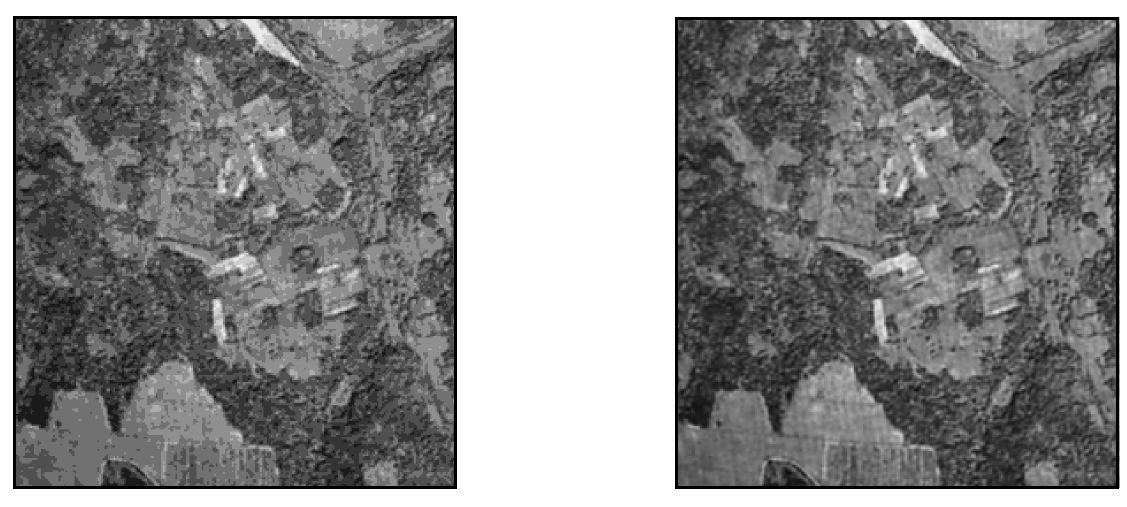
\includegraphics[width=.8\textwidth]{Fuentes_datos/Resolucion_radiometrica.png}
\caption{\small Dos imagenes con distinta resoluci�n radiom�trica (de izquierda a derecha, 8 y 256 niveles, respectivamente).}
\label{Fig:Resolucion_radiometrica} 
\end{figure}

	\item \textbf{Resoluci�n temporal}. Indica el tiempo que tarda el sensor en volver a tomar una imagen de una misma zona.  Tiene sentido en el caso de sensores orbitales, que funcionan por ciclos, y tras concluir este ciclo,  vuelven a comenzar la toma de im�genes en el mismo punto. En cada ciclo, el sensor cubre toda la superficie terrestre <<barriendo>> esta en franjas sucesivas.
	
	La resoluci�n temporal depende de la altura a la que se encuentra la plataforma que monta el sensor, as� como la resoluci�n espacial. Si el tama�o de las im�genes es reducido (GIFOV peque�o), las franjas son m�s estrechas y se requieren m�s para cubrir toda la superficie y volver a comenzar el ciclo, con lo que la resoluci�n espacial ser� menor.
\end{itemize}

Parece l�gico pensar que lo ideal en toda circunstancia ser�a disponer de im�genes procedentes de sistemas con altas resoluciones en cualquiera de las clases anteriores. De esta forma, tendr�amos im�genes con gran detalle espacial, espectral y radiom�trico, y actualizadas frecuentemente. No obstante, la tecnolog�a actual no dispone de elementos que ofrezcan resoluciones elevadas en todas las magnitudes del proceso, y en la creaci�n de los sensores se favorecen unas en detrimento de otras. Algunas resoluci�n presentan adem�s un cierto antagonismo, como hemos visto para las resoluciones espacial y temporal, con lo que no resulta viable que ambas sean elevadas simult�neamente.

As�, existen sensores con, por ejemplo, gran resoluci�n espacial, en los cuales la resoluci�n espectral no es tan elevada. Por el contrario, los sensores con mayor resoluci�n espectral no suelen ofrecer un nivel de detalle espacial tan elevado como los anteriores. En ocasiones, una misma plataforma puede montar a bordo varios sensores, de tal forma que el conjunto de ellos ofrezca informaci�n detallada de forma global, pero un �nico sensor no proporciona resoluci�n elevada en todas las variables.

Otro tipo de circunstancias relativas al sensor afectan igualmente a las resoluciones. Por ejemplo, aquellos sensores que trabajan con radiaciones de poca energ�a (en la regi�n de las microondas) y son de tipo pasivo requieren una amplia extensi�n para recoger la suficiente energ�a como para poder ser detectada por dicho sensor. Por esta raz�n, su resoluci�n espacial suele ser baja. 

A la hora de utilizar im�genes de teledetecci�n, debe considerarse qu� tipo de resoluci�n  resulta de mayor inter�s para el proyecto que se lleva a cabo, teniendo en cuenta la escala de trabajo o el objetivo final que se persigue con el an�lisis a realizar, entre otros factores. En base a esto, se escoger� uno u otro producto, que ser� el que ofrezca los valores de resoluci�n m�s adecuados en conjunto.

Si se pretende localizar elementos de peque�o tama�o, es imprescindible trabajar con altas resoluciones espaciales. Si lo que se desea es clasificar una serie de zonas en funci�n de sus caracter�sticas, la resoluci�n espectral debe ser alta, ya que, como veremos, se usa la informaci�n de todas las bandas para dar esa clasificaci�n, y un n�mero mayor de bandas dar� como resultado una mayor precisi�n.\index{Bandas}

De igual, modo, la detecci�n de cambios de intensidad en una banda hace necesario que se trabaje con una buena resoluci�n radiom�trica, pero si lo que se desea es estudiar esos cambios a lo largo de un periodo corto de tiempo, trabajar con un sensor con gran resoluci�n temporal se hace imprescindible.

En cada caso, las circunstancias particulares del trabajo condicionan la elecci�n de uno u otro sensor, puesto que, como se ha dicho, un �nico sensor no ofrece elevadas resoluciones en todas las variables.

La utilizaci�n simult�nea de datos de varios sensores en un proyecto es una alternativa en ciertos casos. Como veremos, existen t�cnicas que permiten combinar im�genes con alta resoluci�n espacial e im�genes con alta resoluci�n espectral, con objeto de obtener nuevas im�genes que combinen lo mejor de ambas y ofrezcan un nivel de detalle conjunto mayor. Estas t�cnicas realizan el proceso conocido como \emph{fusi�n de im�genes}, el cual trataremos en el apartado  \ref{Fusion_imagenes}, m�s adelante en este libro. \index{Im�genes!fusi�n de}\index{Fusi�n de im�genes}

Adem�s de lo anterior, un �nico sensor montado a bordo de un sat�lite puede operar en varios \emph{modos} distintos. Es habitual que un sensor multibanda pueda registrar tambi�n im�genes de una sola banda, recogiendo en ella la intensidad de la radiaci�n correspondiente a todo el espectro visible, de tal forma que genere una representaci�n visual real. Estas se suelen representar habitualmente en escala de grises, resultando una imagen en blanco y negro.

Las im�genes de este tipo se conocen como \emph{pancrom�ticas}\footnote{El t�rmino \emph{pancrom�tico} deriva de la fotograf�a cl�sica, conoci�ndose as� al tipo de pel�cula sensible a todas las longitudes de onda del visible. Por similitud de conceptos, se emplea el t�rmino tambi�n para hacer referencia a las im�genes digitales monobanda generadas por sensores seg�n lo comentado anteriormente}, y suelen tener mayor resoluci�n espacial, por lo que pueden emplearse para la fusi�n de im�genes se�alada anteriormente. As�, un mismo sensor provee todos los datos necesarios para llevar a cabo ese proceso, tanto la imagen de gran resoluci�n espacial (la pancrom�tica) como la de gran resoluci�n espectral (la imagen multibanda).
\index{Im�genes!pancrom�ticas}

\subsection{Principales sensores y productos}

El n�mero de diferentes productos provenientes de la teledetecci�n es muy elevado en la actualidad. Ahora que ya conocemos los fundamentos del proceso y las principales caracter�sticas de un sistema de teledetecci�n, es interesante mostrar un peque�o resumen de los principales productos disponibles. En ocasiones, desconocer la existencia de productos adecuados puede suponer la realizaci�n incorrecta o de modo ineficaz de un proyecto SIG, y dada la gran variedad existente, esto sucede con frecuencia. 

A continuaci�n se relacionan algunos de los sistemas de teledetecci�n principales y las caracter�sticas de sus productos.

\begin{itemize}
	\item \textbf{LANDSAT} \cite{webLandsat}. Se trata de un programa completo de adquisici�n de datos mediante teledetecci�n, que ha lanzado hasta la fecha un total de siete sat�lites entre 1972 y 1999. Por ello, el volumen de datos recogido es enorme, y lo convierte en una de las fuentes de datos m�s ricas  de entre las existentes en la actualidad. \index{Landsat}

	El �ltimo sat�lite, LANDSAT 7, tiene una �rbita helios�ncrona y una resoluci�n temporal de 16 d�as. A bordo de �l se monta el sensor ETM+\footnote{Enhanced Thematic Mapper Plus}, que permite la obtenci�n de im�genes pancrom�ticas con resoluci�n de 15 metros, e imagenes multibanda con resoluci�n de 60 metros. El sensor recoge un total de 8 bandas, y el tama�o de la imagen es de 170 $\times$ 183 km.

	Los sensores TM\footnote{Thematic Mapper} y MSS \footnote{Multispectral Scanner} se montan a bordo del sat�lite LANDSAT 5, todav�a en funcionamiento y con una resoluci�n temporal de 16 d�as. El sensor TM ofrece im�genes multibanda de 7 bandas con resoluci�n de 30 metros, excepto en la banda del infrarrojo t�rmico, donde la resoluci�n es de 120 metros. Las im�genes tienen un tama�o de 185 $\times$ 172 km.\index{TM (sensor)}\index{MSS(sensor)}
	\item \textbf{IKONOS} \cite{webIkonos}. Este sat�lite, lanzado en 1999, monta un sensor con resoluci�n de 1 metro para im�genes pancrom�ticas y 4 metros para im�genes multibanda (4 bandas). Las im�genes cubren una �rea de 11 $\times$ 11 km y el sat�lite tiene una resoluci�n temporal de entre 3 y 5 d�as.\index{IKONOS}
	\item \textbf{SPOT}\footnote{Satellite Pour l' Observation de la Terre} \cite{webSPOT}. Un conjunto de sat�lites lanzados inicialmente por la agencia espacial francesa, con especial �nfasis en la recogida de informaci�n relativa a variables ambientales. De los cinco puestos en �rbita, dos siguen actualmente en funcionamiento. El �ltimo de ellos, lanzado en 2002, monta el sensor HRG con capacidad de producir im�genes pancrom�ticas con resoluci�n entre 2,5 y 5 metros, e im�genes multibanda con resoluci�n de 10 metros. El periodo de revisita es de entre 1 y 4 d�as.
	Es de destacar que el sensor permite inclinaciones de hasta 27\degree respecto al nadir hacia ambos lados, por lo que puede cubrir una banda m�s ancha y tomar im�genes fuera del �rea determinada en cada instante por la �rbita.\index{SPOT}\index{Satellite Pour l' Observation de la Terre}
	\item \textbf{QuickBird}. \cite{webQuickbird}. Ofrece im�genes en pancrom�tico y multibanda (azul, verde, rojo e infrarrojo cercano). Las primeras tiene una resoluci�n de 60 cm y las multibanda de 2,4 metros, aunque combinando las dos ofrece im�genes en color con 60 cm de resoluci�n. 
	La �rbita del sat�lite es helios�ncrona y la resoluci�n temporal var�a entre los 3 y 7 d�as. Cada imagen cubre una superficie de 16,5 $\times$ 16,5 km.\index{QuickBird}
	\item \textbf{Aqua y Terra}. Dos sat�lites lanzados por la NASA dentro de un proyecto de �mbito internacional para la observaci�n de la Tierra. Cada uno de ellos monta una serie de diversos sensores, que recogen informaci�n relativa al ciclo hidrol�gico (en el caso del Aqua) y la superficie terrestre (en el caso del Terra). Entre estos sensores cabe destacar el MODIS, a bordo de ambos, o el ASTER, a bordo del sat�lite Terra. ASTER \footnote{Advanced Spaceborne Thermal Emission and Reflection Radiometer} recoge informaci�n en 14 bandas distintas, con una resoluci�n entre 15 y 90 metros, mientras que MODIS\footnote{Moderate Resolution Imaging Spectroradiometer} es un sat�lite de menor resoluci�n espacial (250, 500 o 1000 metros seg�n la banda ), 36 bandas y una resolucion temporal de 1 a 2 d�as. \index{Aqua}\index{Terra}\index{NASA}\index{ASTER}\index{MODIS}

	Adem�s de los datos directos de los sensores, se proporcionan de forma gratuita numerosos productos derivados, lo que lo convierte en una fuente de datos de primer orden para un gran n�mero de aplicaciones, especialmente las relacionadas con el estudio del medio, la vegetaci�n, etc. En la direcci�n Web \cite{webModisData} pueden obtenerse tanto datos originales como productos derivados.
	\item \textbf{NOAA--AVHRR}\footnote{Advanced Very High Resolution Radiometer}. Se encuentra principalmente enfocado al estudio de los oc�anos, aunque sus datos pueden aplicarse en muchos m�s estudios. El sensor tiene una resoluci�n de 1,1 km, y proporciona im�genes de 5 bandas en las regiones del infrarrojo y el visible. La resoluci�n temporal es de medio d�a, produciendo una imagen nocturna y otra diurna.\index{NOAA-AVHRR}
	\item \textbf{RADARSAT}. Desarrollado por la Agencia Espacial Canadiense, monta un radar de apertura sint�tica (SAR), y su principal prop�sito es el control de las variaciones ambientales y de los recursos naturales. M�s informaci�n en \cite{webRADARSAT}.\index{RADATSAT}\index{Radar de Apertura Sint�tica}\index{SAR}
	\item \textbf{ERS--1 y ERS--2}. Desarrollados por la Agencia Espacial Europea. Al igual que el anterior, ambos est�n pensados para la observaci�n medioambiental, y montan tanto sensores activos como pasivos. M�s informaci�n en \cite{webERS2}.\index{ERS--1}\index{ERS--2}
	\item \textbf{SRTM}. La misi�n SRTM\footnote{Shuttle Radar Topography Mission} es un proyecto internacional de gran envergadura destinado a la creaci�n de una cobertura de elevaciones a nivel mundial. Utilizando sensores basados en radar montados sobre una lanzadera espacial, se realiz� un vuelo global de la superficie terrestre a lo largo de 11 d�as, recogiendo el relieve de todas las zonas situadas entre los 56 grados sur y los 60 grados norte de latitud. La resoluci�n de los datos obtenidos es de un segundo de arco (aproximadamente 30 metros), aunque solo se encuentran disponibles para Estados Unidos, siendo de unos 90 metros en el resto de zonas. Los datos SRTM se pueden descargar gratuitamente en \cite{webSRTMDownload}. M�s informaci�n sobre el proyecto puede encontrarse en \cite{webSRTM}. \index{SRTM}\index{Shuttle Radar Topographic Mission}
\end{itemize}

\section{Cartograf�a impresa. Digitalizaci�n}

\index{Digitalizaci�n}

La primera fuente de cartograf�a de la que se dispon�a en las etapas iniciales de los SIG era la  cartograf�a impresa. No se trataba de elementos creados pensando en su utilizaci�n dentro de un SIG y, de hecho, su estructura no es, como veremos, la m�s adecuada para ser incorporados como datos de trabajo en un SIG. Se trata, por tanto, de una clara fuente secundaria de datos espaciales. Aun as�, esta fuente era la fuente principal de informaci�n cartogr�fica disponible entonces, y su uso ha sido desde esos tiempos una constante dentro del �mbito SIG.

A pesar de que hoy en d�a disponemos de otras fuentes cartogr�ficas, la cartograf�a impresa sigue siendo b�sica para trabajar con un SIG, ya que existe mucha informaci�n que todav�a solo se encuentra en este formato. De una u otra forma, es probable que un proyecto SIG implique en alg�n punto de su desarrollo la necesidad de recurrir a cartograf�a impresa y tratar esta para su inclusi�n dentro de un SIG.

Cuando hablamos de cartograf�a impresa, no hay que pensar �nicamente en mapas o planos, sino tambi�n en im�genes tales como fotograf�as a�reas, las cuales, dependiendo de su antig�edad, pueden encontrarse disponibles tan solo en formato impreso, como hemos visto. Mientras que resulta posible adquirir estas en formato digital cuando se trata de fotograf�as m�s actuales, la tomadas por m�todos anal�gicos correspondientes a vuelos m�s antiguos solo pueden adquirirse por regla general como un producto impreso.

Los procesos que permiten obtener un producto digital a partir de esas im�genes son costosos en tiempo y dinero, y es por ello que no todos los proveedores de estas ofrecen la posibilidad de adquisici�n de un producto digital. En esta secci�n veremos esos procesos, tanto si partimos de un mapa o plano como si partimos de una imagen o cualquier otro documento impreso que pueda contener informaci�n cartogr�fica, susceptible de ser convertida en una o varias capas seg�n se requieren para el trabajo en un SIG.

Ya conocemos los dos modelos de datos con los que trabajamos en un SIG: el modelo r�ster y el modelo vectorial. Tanto mapas como fotograf�as a�reas pueden servir como fuente de informaci�n para crear o bien capas r�ster o bien capas vectoriales, ya que la informaci�n que contienen puede de igual modo representarse seg�n uno u otro modelo (debe recordarse que, como se mencion� en el cap�tulo \ref{Tipos_datos}, puede convertirse una capa r�ster en vectorial y viceversa mediante algoritmos que detallaremos m�s adelante en este libro).\index{Conversi�n!r�ster--vectorial}

Un mapa o plano sobre un soporte impreso, sin embargo, dista considerablemente de ese concepto de capa con el que trabajamos en un SIG. Suele contener informaci�n sobre distintas variables, tales como carreteras, elevaci�n, n�cleos urbanos, uso de suelo, y todas ellas en un �nico elemento cartogr�fico. Esas variables, que en un SIG manejar�amos como capas independientes, se presentan como un conjunto que, seg�n el uso que queramos darle, va a ser mucho m�s conveniente disgregar en base a esas distintas variables.

Si pensamos en una fotograf�a a�rea, esta puede considerarse como una simple imagen dentro de un SIG, y como vimos en el cap�tulo \ref{Tipos_datos}, las im�genes se adaptan al modelo de representaci�n r�ster. Por otra parte, en esa imagen existir�n elementos tales como carreteras, r�os o �rboles, los cuales se representan mejor seg�n el modelo vectorial. En funci�n de qu� informaci�n nos interese tener dentro de un SIG o el modelo de representaci�n preferente que queramos manejar, las operaciones que debemos llevar a cabo ser�n unas u otras.

Este conjunto de operaciones posibles se conocen como de \emph{digitalizaci�n}, y en funci�n de la forma en que se desarrollen podemos distinguir los siguientes tipos:

\begin{itemize}
	\item Digitalizaci�n autom�tica 
	\item Digitalizaci�n manual
\end{itemize}

\index{Digitalizaci�n!tipos}

En la digitalizaci�n autom�tica, el sistema (inform�tico o mec�nico) se encarga de generar los elementos digitales que ya podremos incorporar a un SIG, ahorrando trabajo al operador al automatizar la tarea. Este tipo de digitalizaci�n es muy habitual para el caso de obtener un resultado r�ster mediante el proceso de \emph{escaneo}\index{Escaneo}. Tambi�n resulta posible automatizar la digitalizaci�n para el caso vectorial, aunque requiere cierta labor por parte del operario y no es un proceso tan sencillo, pudiendo obtenerse resultados desiguales. 

La digitalizaci�n manual requiere por parte del operario una definici�n expl�cita de los elementos a crear, y es por ello �nicamente adecuada para obtener un resultado vectorial, traz�ndose las entidades (sean estas puntos, l�neas o pol�gonos) manualmente mediante alg�n sistema que permita esa introducci�n de datos. 

La elecci�n de uno u otro tipo de digitalizaci�n no depende solo del tipo de capa que se desee obtener. Tanto la digitalizaci�n manual como la autom�tica, tienen cada una de ellas su propias ventajas. En el caso r�ster la opci�n manual no es viable, pero al digitalizar un mapa para obtener una capa vectorial puede ser interesante optar por una o otra metodolog�a en funci�n de las circunstancias. 

La digitalizaci�n manual es mucho m�s costosa y su resultado es muy variable en cuanto a su precisi�n espacial, ya que depende en gran medida de la experiencia del operario y de las condiciones de este (cansancio, circunstancias personales, etc.). Por el contrario, e independientemente del operario, el reconocimiento de las entidades es altamente fiable (si se trata de un mapa, este ha sido dise�ado para ser interpretado por una persona, por lo que esta reconocer� sus elementos sin dificultad y con total fiabilidad). 

Asimismo, un proceso autom�tico, en caso de proceder de forma correcta, tendr� una exactitud absoluta y <<clonar�>> con absoluta fidelidad los elementos del mapa impreso. Esto resulta una ventaja a la hora de obtener una gran precisi�n, pero impide que en el proceso de digitalizaci�n se puedan corregir errores existentes en el documento original. Un operario puede advertir esos errores y corregirlos a medida que digitaliza. Un sistema autom�tico, por el contrario, no puede.
 
\subsection{Digitalizaci�n manual}
\label{Digitalizacion_manual}\index{Digitalizaci�n!manual}

La digitalizaci�n manual es la forma m�s b�sica de crear informaci�n digital a partir de un documento cartogr�fico impreso. Un operario trabaja directamente sobre la fuente cartogr�fica y su trabajo se traduce en la creaci�n de una nueva capa, gracias a la utilizaci�n de un equipo que es capaz de convertir su trabajo en la informaci�n necesaria para crear dicha capa.

En el modelo de representaci�n r�ster, los elementos b�sicos son las celdas, que forman una malla regular que puede presentar un numero muy elevado de estas. Una definici�n manual de las caracter�sticas de cada una de esas celdas resulta inviable, por lo que la digitalizaci�n de un documento cartogr�fico impreso para la obtenci�n de una capa r�ster a partir de ella de forma manual no es factible.

Por el contrario, se puede realizar con cierta sencillez la digitalizaci�n de una entidad vectorial, trazando la forma de esta o, en caso de ser una entidad de tipo punto, sencillamente indicando su localizaci�n. Cuando el n�mero de entidades es elevado, el proceso puede llevar tiempo y ser tedioso, pero en todo caso sigue resultando una forma sencilla y accesible de crear una capa vectorial a partir de otra fuente de datos.

Para llevar a cabo ese trazado de la entidad, se necesita emplear alg�n equipo que recoja la informaci�n introducida por el operador. Existen dos alternativas principales: utilizar un equipo especializado dise�ado espec�ficamente para la digitalizaci�n, o bien digitalizar utilizando las funciones de edici�n de un GIS, realizando todo el proceso dentro de este y sin m�s herramientas que el propio ordenador y un dispositivo se�alador como el rat�n.

\subsubsection{Con equipo especializado (\emph{heads--down})} \label{heads-down}

\index{Heads--down}

La forma tradicional de proceder a la digitalizaci�n manual de entidades es utilizando equipos y perif�ricos expresamente dise�ados para llevar a cabo esta tarea. La \emph{tableta digitalizadora} (Figura \ref{Fig:Tableta_digitalizadora}) es la herramienta fundamental para este trabajo.\index{Tableta digitalizadora}

\begin{figure}[!hbt]   
\centering
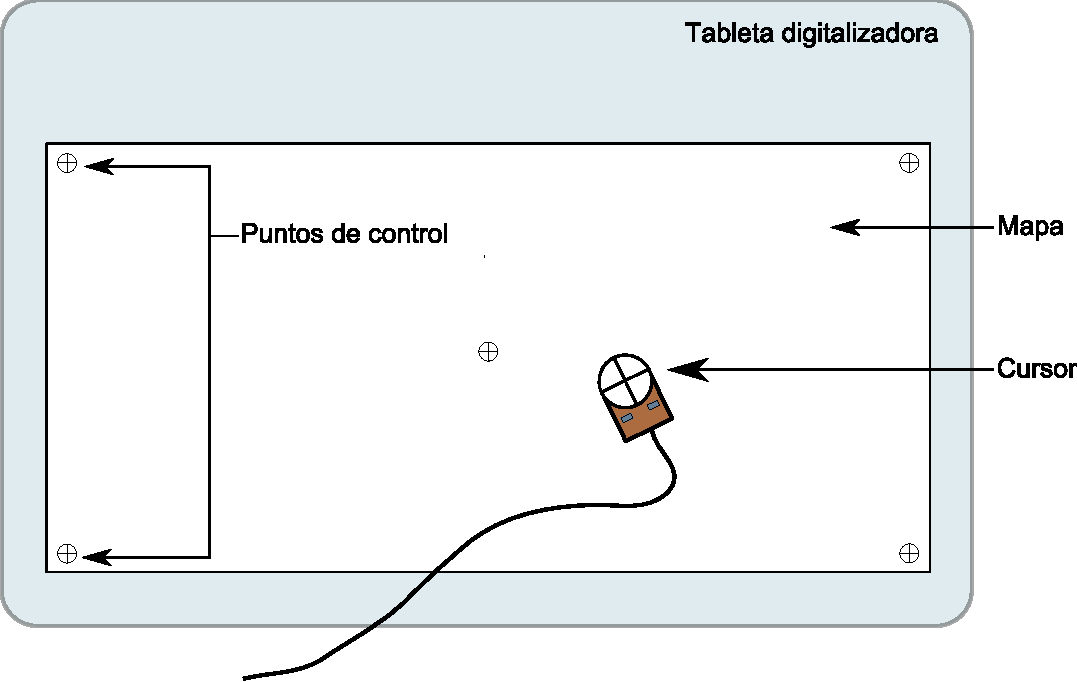
\includegraphics[width=.8\textwidth]{Fuentes_datos/Tableta_digitalizadora.pdf}
\caption{\small Esquema de una tableta digitalizadora y los elementos del proceso de digitalizaci�n.}
\label{Fig:Tableta_digitalizadora} 
\end{figure}

Se trata de una superficie plana a modo de atril, sobre la cual se sit�a el documento cartogr�fico a digitalizar, y sobre este se van trazando las distintas entidades con un cursor. Este cursor registra los movimientos del operario, convirtiendo las posiciones del cursos en coordenadas reales, que son las que van a constituir la entidad digitalizada. El trabajo del operario consiste en seguir con el cursor las formas de las distintas entidades, como si las estuviera calcando, de modo que indique al sistema las geometr�as que se quieren definir.

El proceso de digitalizaci�n implica los siguientes pasos \cite{Heywood1998Longman}:

\begin{itemize}
	\item \textbf{Registro}. La etapa fundamental del proceso, que garantiza que las coordenadas de las entidades digitalizadas sean correctas. El mapa se ha de adherir a la tableta de modo firme, normalmente con cinta adhesiva u otro medio similar, y se�alar en �l unos \emph{puntos de control} de coordenadas conocidas. Ser� en base a estos como se calcularan las restantes coordenadas de las entidades que el operario defina mediante el cursor. Habitualmente se utilizan como puntos de control las esquinas y alg�n punto central del mapa. Es importante que en el proceso de registro el mapa no presente dobleces o deterioros que puedan inducir errores en el c�lculo de coordenadas posteriores.\index{Puntos!de control}
	\item \textbf{Digitalizaci�n}. De entidades puntuales, lineales y poligonales.
	\item \textbf{Asignaci�n de atributos}. A cada una de las entidades digitalizadas se le a�aden sus correspondientes propiedades. Este paso no se realiza ya con la tableta digitalizadora.
	En el caso m�s general, estos atributos se introducen manualmente con el teclado o se toman, por ejemplo, de una base de datos. Un caso particular, no obstante, es el de la digitalizaci�n de curvas de nivel. Una vez que estas han sido digitalizadas, no es necesario asignar valores individualmente a cada una de las lineas, ya que entre ellas existe una relaci�n que puede aprovecharse para simplificar el establecimiento de una cota correspondiente a cada una. Estableciendo la elevaci�n de una y la direcci�n en que la elevaci�n aumenta, pueden sistem�ticamente asignarse elevaciones a las curvas que aparecen seg�n se avanza en dicha direcci�n. Los SIG m�s populares presentan habitualmente herramientas que facilitan este proceso.
\end{itemize}

Esta forma de digitalizar se conoce como <<cabeza abajo>> (\emph{heads--down}), en referencia a la posici�n del operario a la hora de trabajar sobre la tableta.

Se distinguen dos formas principales de registro de puntos:

\begin{itemize}
	\item \textbf{Manual}. El usuario debe ir marcando uno por uno todos los puntos que desee incorporar a la entidad digitalizada. Por ejemplo, para el caso de una l�nea, debe ir deteniendo el rat�n regularmente en aquellos puntos que considere de inter�s, y sobre ellos pulsando los botones del cursor para indicar al sistema que ha de registrar dichos puntos.
	\item \textbf{Semiautom�tica}. El operario simplemente desliza el cursor definiendo la forma de los entidades, y el propio sistema se encarga de almacenar puntos regularmente seg�n un intervalo de tiempo definido. Esto permite un ahorro de tiempo considerable y una correcta densidad de puntos recogidos para cada entidad.	
\end{itemize}

Las tabletas digitalizadoras son elementos caros, motivo por el cual se tiende a favorecer en la actualidad la digitalizaci�n en pantalla, que presenta adem�s otra serie de ventajas adicionales, como seguidamente veremos.
 
\subsubsection{En pantalla (\emph{heads--up})}

\index{Heads--up}

La otra forma de digitalizar elementos es utilizando las capacidades de edici�n de un SIG. Estas capacidades son heredadas de las aplicaciones de dise�o asistido por ordenador (CAD)\index{CAD}, y permiten <<dibujar>> en la pantalla del ordenador entidades y formas tales como los puntos, l�neas y rectas que constituyen los objetos en el modelo de representaci�n vectorial.

En este proceso se parte igualmente de un capa base, generalmente una imagen, y bas�ndose en ella se van definiendo los objetos, <<dibuj�ndolos>> sobre la pantalla, una vez m�s como si se calcara aquello que puede visualizarse en dicha imagen. El hecho de que un SIG nos permita tener varias capas simult�neamente y visualizarlas a voluntad, facilita el proceso de digitalizaci�n. Tambi�n lo facilita el poder tener varias im�genes sobre el fondo (cada una de ellas como una capa individual), de modo que podemos cubrir un �rea m�s amplia que la de una simple hoja de mapa o una �nica imagen.

En este proceso, no partimos en realidad de un documento cartogr�fico anal�gico, pues ya ha sido necesario digitalizarlo de alguna forma para incorporarlo en un SIG. El proceso es una digitalizaci�n de las entidades como tales, pero la informaci�n ya ha de estar en formato digital, aunque no en el modelo de representaci�n vectorial, sino en el modelo r�ster. Por ello, puede utilizarse como capa de partida una imagen originalmente en formato digital o bien una imagen originalmente en formato impreso. En este ultimo caso, la imagen ha debido digitalizarse previamente mediante un proceso de \emph{escaneo}, el cual se tratar� en la siguiente secci�n.

En la figura \ref{Fig:Digitalizacion_en_pantalla} puede verse un ejemplo de la digitalizaci�n de una imagen en pantalla.

\begin{figure}[!hbt]   
\centering
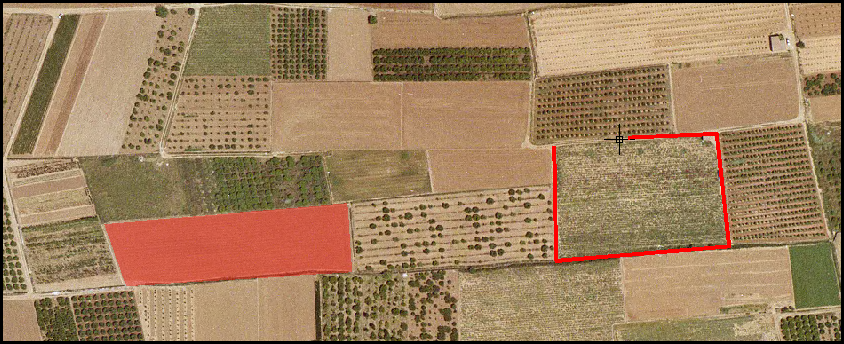
\includegraphics[width=.8\textwidth]{Fuentes_datos/Digitalizacion_en_pantalla.png}
\caption{\small Digitalizaci�n en pantalla. En rojo, pol�gono ya digitalizado. Las lineas rojas indican un nuevo pol�gono, actualmente en edici�n}
\label{Fig:Digitalizacion_en_pantalla} 
\end{figure}

En la figura, sobre una imagen a�rea en color se digitalizan las distintas parcelas que pueden distinguirse en esta. Del mismo modo, pueden digitalizarse curvas de nivel en un mapa escaneado, u otras entidades tales como r�os, lagos o v�as de comunicaci�n sobre una fotograf�a a�rea, entre muchas otras. La digitalizaci�n en pantalla puede incluso utilizarse teniendo como base no una imagen, sino capas de cartograf�a vectorial o cualquier capa de datos que aporte alg�n tipo de informaci�n que pueda delinearse con las mismas herramientas de edici�n.

La digitalizaci�n en pantalla se conoce tambi�n como digitalizaci�n <<cabeza arriba>> (\emph{heads--up}), ya que el operador centra su atenci�n en la pantalla, con una postura bien distinta a la que se tiene al trabajar con una tableta digitalizadora.

Frente a dicho trabajo con tableta digitalizadora, la digitalizaci�n en pantalla tiene las siguientes ventajas:

\begin{itemize}
	\item \textbf{Menor coste}. No se requiere equipo especializado de alto coste, ya que basta con un ordenador personal. 
	\item \textbf{Posibilidad de dividir el trabajo}. Cuando se trabaja con un mapa sobre una tableta digitalizadora, este mapa no puede ser utilizado por otro operario. Sin embargo, el uso de una capa digital dentro de un SIG como base para la digitalizaci�n, permite que varios operarios trabajen con ella simult�neamente y se repartan el trabajo.
	\item \textbf{Posibilidad de correcci�n y edici�n precisa}. Las mismas capacidades que se usan para trazar las distintas entidades puede emplearse para corregir o modificar estas una vez que estas ya han sido digitalizadas (Figura \ref{Fig:Correccion_digitalizacion}), resultando esto en un proceso de digitalizaci�n m�s flexible.
	\item \textbf{Posibilidad de ampliaci�n}. Para cartograf�as de baja calidad, puede ser dif�cil obtener precisi�n si se trabaja directamente sobre el mapa, as� como si los elementos a digitalizar son peque�os, requiri�ndose del operador un esfuerzo visual adicional. Las capacidades que tiene todo SIG para ampliar una imagen (\emph{zoom}) permiten superar esta dificultad y trabajar a distintas escalas seg�n la precisi�n del trabajo a realizar o las caracter�sticas de los objetos digitalizados.
	\item \textbf{Mayor precisi�n}. La capacidad de resoluci�n del ojo humano es mucho menor que la resoluci�n de las im�genes (v�ase m�s adelante el apartado \ref{Condiciones_digitalizacion}). Esto, unido a lo mencionado en el punto anterior, permite aprovechar mejor la informaci�n de la fuente original, y que los resultados obtenidos en la digitalizaci�n de esta sean m�s fieles a ella.
	\item \textbf{Mayor comodidad para el operario}. La postura del operario es m�s adecuada cuando se digitaliza sobre la pantalla, permitiendo unas mejores condiciones. Esto que se traduce en menor cansancio y ello indirectamente comporta resultados m�s precisos.
\end{itemize}

\begin{figure}[!hbt]   
\centering
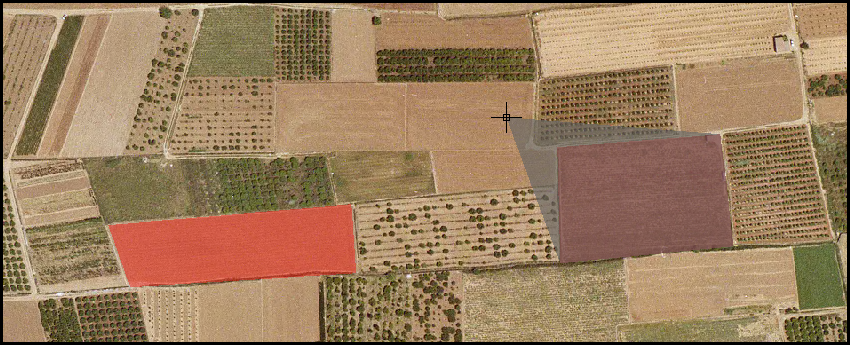
\includegraphics[width=.8\textwidth]{Fuentes_datos/Correccion_digitalizacion.png}
\caption{\small Correcci�n de entidades con las funciones de edici�n de un SIG. El pol�gono de la derecha se encuentra en edici�n, siendo modificado uno de sus v�rtices.}
\label{Fig:Correccion_digitalizacion} 
\end{figure}

Para conocer con m�s detalle las capacidades b�sicas de edici�n de un SIG, as� como las restantes capacidades que contribuyen a su vez a facilitar la labor de edici�n, cons�ltese el capitulo \ref{SIGs_escritorio}.

\subsection{Digitalizaci�n autom�tica}\index{Digitalizaci�n!autom�tica}

La digitalizaci�n autom�tica limita el trabajo del operario, ya que este no es responsable directo de definir las propiedades de los elementos que se digitalizan. Este tipo de digitalizaci�n es la  habitual en el caso de generar una capa r�ster, aunque tambi�n pueden obtenerse capas vectoriales procesando de modo autom�tico cartograf�a impresa. 

Este segundo caso, no obstante, requiere una cartograf�a en condiciones especiales, no siendo adecuada para todo tipo de mapas. En caso de no presentarse esas condiciones, los resultados de la digitalizaci�n no son �ptimos, y requieren posteriormente un gran trabajo de correcci�n y supervisi�n.

\subsubsection{Escaneo}
\label{Escaneo}

\index{Escaneo}

El escaneo es el proceso de digitalizaci�n que convierte una imagen impresa (anal�gica) en una imagen digital \cite{Jackson1991Longman}. El resultado de este proceso es, por tanto, y desde el punto de vista de un SIG, una capa r�ster. Pueden escanearse tanto mapas como fotograf�as a�reas, operando en ambos casos de un modo similar y con las mismas consideraciones, pues el objeto del proceso es el mismo: la conversi�n del documento impreso en un documento digital que pueda utilizarse dentro de un SIG o cualquier otro software tal como, por ejemplo, un software de tratamiento de im�genes.

El dispositivo fundamental para realizar este proceso es el \emph{esc�ner}. Este se compone de una \emph{cabeza} sobre la que se monta un sensor, y un soporte sobre el que se desplaza o bien la cabeza o bien el documento a escanear, de tal modo que durante el proceso de escaneo esta recorre todo el documento, recogiendo la informaci�n de toda su extensi�n.\index{Esc�ner}

Este proceso de \emph{barrido} se realiza en una �nica ocasi�n, aunque dispositivos m�s antiguos pueden hacerlo en tres ocasiones a la hora de escanear documentos en color. Aunque lo habitual es la creaci�n de una imagen en color, tambi�n  pueden obtenerse im�genes en blanco y negro o en escala de grises.

Aunque existen esc�neres espec�ficamente dise�ados para el trabajo con documentos cartogr�ficos, estos son dispositivos muy especializados y de muy elevado coste. Los esc�neres m�s gen�ricos, pensados para el trabajo con todo tipo de im�genes y para todo tipo de usos, pueden no obstante emplearse de igual modo para escanear tanto mapas como im�genes a�reas con resultados aceptables, utiliz�ndose con frecuencia.

Existen tres tipos principales de esc�neres:

\begin{itemize}
	\item \textbf{De sobremesa} (\emph{flat--bed}). Los habituales para el uso dom�stico o el escaneo de im�genes de peque�o formato, aunque tambi�n existen de mayor tama�o. El documento a escanear se sit�a sobre una placa de cristal bajo la que se desplaza la cabeza con el sensor. Puede verse uno de estos esc�neres en la figura \ref{Fig:Escaner_sobremesa}.\index{Flat--bed}
	\item \textbf{De tambor}. El mapa se sit�a sobre un tambor que rota, mientras que la cabeza se mantiene fija. La figura \ref{Fig:Escaner_tambor} muestro uno de estos esc�neres.
	\item \textbf{Alimentados}. El sensor se mantiene fijo y el documento se desplaza mediante un mecanismo de arrastre, de forma similar a como avanza el papel en una impresora dom�stica. Salvo que dispongan de mecanismos espec�ficos para corregir esta circunstancia, suelen presentar importantes distorsiones geom�tricas causadas por un desplazamiento impreciso del papel.
\end{itemize}

\begin{figure}[!hbt]   
\centering
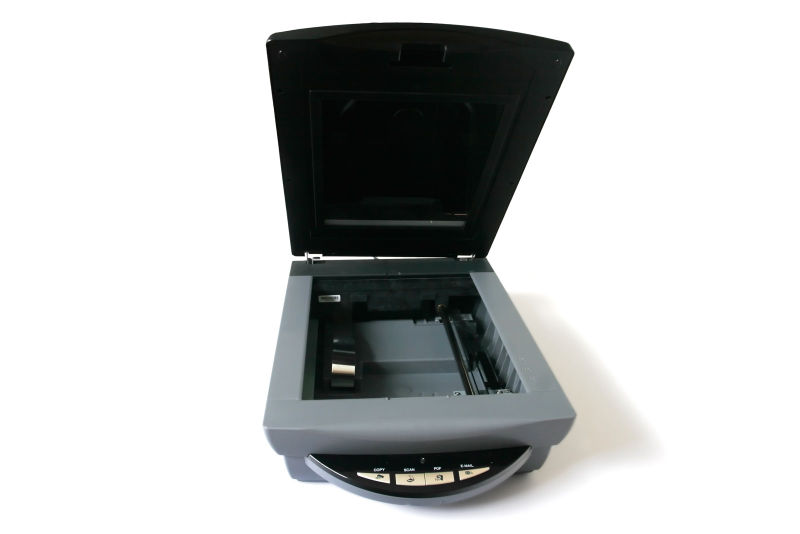
\includegraphics[width=.5\textwidth]{Fuentes_datos/Escaner_sobremesa.png}
\caption{\small Esc�ner de sobremesa (tomado de Wikipedia)}
\label{Fig:Escaner_sobremesa} 
\end{figure}

\begin{figure}[!hbt]   
\centering
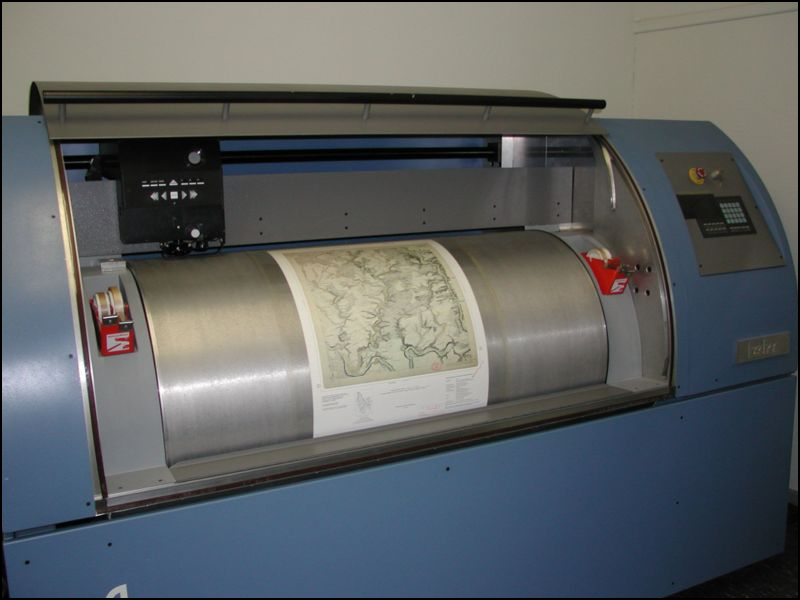
\includegraphics[width=.5\textwidth]{Fuentes_datos/Escaner_tambor.png}
\caption{\small Esc�ner de tambor (fotograf�a: Stefan Kuehn)}
\label{Fig:Escaner_tambor} 
\end{figure}

Los par�metros b�sicos que definen las caracter�sticas de un esc�ner son la resoluci�n espacial y la resoluci�n radiom�trica. La primera de estas de mide habitualmente en \emph{puntos por pulgada}\footnote{\emph{Dots per inch}(dpi)} y nos indica el n�mero de puntos (celdas) que el sensor es capaz de tomar por cada unidad de longitud sobre el papel. La resoluci�n radiom�trica, por su parte, indica la capacidad del sensor para distinguir entre dos colores distintos.\index{Dots per inch}\index{Resoluci�n!espacial}\index{Resoluci�n!radiom�trica}

A la hora de trabajar con documentos cartogr�ficos de cara a su posterior utilizaci�n en un SIG, tanto la resoluci�n espacial como la radiom�trica de los esc�neres habituales es en general m�s que suficiente, incluso en ocasiones en aquellos de uso dom�stico. No obstante, es habitual que se presenten distorsiones geom�tricas que suponen un problema importante a la hora de mantener la precisi�n cartogr�fica, y ello exige la utilizaci�n de equipos de mayor calidad si se requiere un resultado de alta precisi�n. Estos equipos no han de ser necesariamente de aquellos pensados para el trabajo con cartograf�a, sino que pueden ser de uso gen�rico, siempre, eso s�, que sean de la calidad necesaria.

La velocidad del esc�ner es otro par�metro importante, pues la preparaci�n de una base de datos cartogr�fica a partir de cartograf�a anal�gica puede llevar un tiempo considerable si el volumen de datos es elevado, ya que el proceso de escaneo es laborioso y requiere de cierto tiempo. El rendimiento del esc�ner y la velocidad a la que puede digitalizar una imagen dada est� en relaci�n directa con la resoluci�n espacial. Un esc�ner posee una resoluci�n nominal (en dpi), que es la resoluci�n m�xima a la que puede trabajar (el detalle m�ximo que puede recoger). No obstante, puede ajustarse la resoluci�n de trabajo en funci�n de las necesidades, y una resoluci�n mayor siempre lleva asociado un tiempo de proceso mayor, ya que el volumen de informaci�n generado es mayor, as� como el detalle que ha de registrarse.\index{Resoluci�n!nominal de un escaner}

Para cada documento existe una resoluci�n �ptima de escaneo en funci�n de las caracter�sticas de este. Esta resoluci�n debe elegirse teniendo en cuenta que el volumen de datos aumenta a medida que empleamos una mayor resoluci�n, buscando un equilibrio adecuado entre ese volumen de datos resultante y la cantidad de informaci�n que recogemos. Asimismo, se ha considerar igualmente el tiempo necesario para escanear el documento, tal como se dijo anteriormente.

El par�metro base es la relaci�n entre el tama�o de p�xel (la longitud real que representa el ancho de un p�xel sobre el terreno) y el tama�o de este p�xel en la imagen (lo que mide esa longitud en el mapa). Las resoluciones habituales utilizadas para el escaneo de fotograf�as a�reas var�an entre los 100 dpi ($\approx 250 \mu m$ cada punto sobre el mapa) y 2500 dpi (($\approx 10 \mu m$ cada punto sobre el mapa) \cite{Welch1996Onward}. Por ejemplo para una resoluci�n de 300 dpi, se tiene:

\begin{equation}
300 \mathrm{dpi} = \frac{300\mathrm{filas}}{2,54 \mathrm{cm\; de\; mapa}} = 118,11 \mathrm{filas/cm\; de\; mapa}
\end{equation}

En un cent�metro cuadrado se tienen $118,11^2\approx13950$ puntos.

Si trabajamos, por ejemplo, con un mapa a una escala 1:50000, tenemos que la distancia real que representa el alto de cada fila es

\begin{equation}
\frac{50000 \mathrm{cm}}{118,11 \mathrm{filas}} = 4,24 \mathrm{metros}/\mathrm{fila}
\end{equation}

Es decir, cada p�xel del mapa representa sobre el terreno un cuadrado de lado 4,24 metros.\index{Pixel}

Con c�lculos similares podemos calcular para cada posible resoluci�n el espacio real que representa, y elegir esta en funci�n del detalle que necesitemos. Como regla general, debe tratar de trabajarse con una resoluci�n que garantice que los objetos que resultan de inter�s de la imagen (por ejemplo, aquellos que van a digitalizarse despu�s manualmente mediante una digitalizaci�n en pantalla con esa imagen) sean distinguibles con claridad. 

En el caso de im�genes a�reas, la resoluci�n de estas medida en pares de lineas por mil�metro puede ser superior y permitir escanear a mayor resoluci�n, aunque ello no es estrictamente necesario, y debe una vez m�s buscarse el equilibrio entre las ventajas y los inconvenientes de trabajar con una resoluci�n m�s elevada.

En \cite{Welch1996Onward} puede encontrarse informaci�n m�s detallada sobre la elecci�n de una resoluci�n �ptima en el escaneo de im�genes a�reas.

Para el caso de mapas, no deben olvidarse los fundamentos cartogr�ficos en base a los cuales se ha creado dicho mapa, que fueron detallados en el cap�tulo \ref{Fundamentos_cartograficos}. Trabajando con una resoluci�n m�s elevada no hace necesariamente que estemos incorporando m�s informaci�n, ya que esta puede no existir en el mapa original. Tendr�amos un volumen de datos m�s elevado que el necesario para recoger toda la informaci�n del mapa.

Una diferencia fundamental entre escanear una hoja de un mapa y una imagen a�rea es la diferencia de tama�o. Los mapas suelen tener tama�os mucho mayores que los de un esc�ner com�n, lo cual obliga a utilizar equipos de gran formato o, en la mayor�a de los casos, contratar servicios de escaneo especializados, ya que estos equipos tiene un coste muy elevado. 

Una soluci�n distinta en el caso de mapas de gran tama�o es el escaneo de la hoja por partes y la posterior uni�n de las distintas partes. En este caso, es necesario asegurarse de que las partes son coherentes entre s� en lo que respecta a las condiciones bajo las que se realiza el escaneo, as� como garantizar que las distintas partes se solapan para que no existan zonas sin datos en la imagen resultante. Adem�s de esto, el solape facilita la localizaci�n de puntos comunes presentes entre partes contiguas, lo que ayuda en la composici�n de todas las partes para dar lugar al resultado global.

Otra diferencia entre trabajar con mapas e im�genes es la relativa al tipo de soporte. En el caso de mapas, el documento original se encuentra siempre impreso en papel. En el caso de fotograf�as a�reas puede presentarse tanto en papel como en diapositiva. Los esc�neres est�n preparados para capturar la imagen tanto por \emph{reflexi�n} (cuando se trabaja con un documento en papel) como por \emph{transmisi�n} (cuando se trabaja con una diapositiva o cualquier otro soporte transparente), por lo que ambos tipos de fuentes pueden utilizarse indistintamente para generar una imagen digital, siendo esta diferencia menos relevante a efectos pr�cticos.

Por �ltimo, un aspecto clave en el escaneo de cartograf�a es la asignaci�n de coordenadas a la capa resultante. Cuando utilizamos una tableta digitalizadora, debemos definir los \emph{puntos de control}, que son los que establecen la referencia geogr�fica en base a la cual se calculan las coordenadas de los elementos que digitalizamos con el cursor. En el caso de escanear un mapa o una fotograf�a a�rea, esa informaci�n est� presente en el mapa en forma de marcas fiduciales o una ret�cula con coordenadas impresas, pero no se digitaliza como tal.\index{Puntos!de control}\index{Marcas fiduciales}

Si simplemente escaneamos el documento, se digitaliza la marca fiducial o la etiqueta que indica las coordenadas, pero tan solo como una imagen, y no como un dato aprovechable por el SIG para otras tareas. En esta imagen, un operador puede ver las coordenadas de un punto, pero si realizamos un proceso de digitalizaci�n vectorial en pantalla utilizando esa imagen, el SIG no tiene forma de calcular las coordenadas de los puntos que introducimos, pues carece de una referencia.

Para que una imagen procedente del escaneo de un documento impreso tenga plena validez y utilidad dentro de un SIG, es necesario a�adirle informaci�n sobre la localizaci�n en el espacio del �rea representada en dicho documento. Este proceso se denomina \emph{georreferenciaci�n}.\index{Georreferenciaci�n}

La georreferenciaci�n es un proceso tratado dentro de este libro en el apartado \ref{Rectificacion}, puesto que no es puramente un proceso que forme parte de la adquisici�n de datos, sino un tratamiento a aplicar una vez que el proceso de digitalizaci�n ha sido realizado. No obstante, es necesario recalcar de nuevo la importancia vital de este proceso, ya que sin �l no resulta posible aprovechar el resultado del escaneo dentro de un SIG.

\subsubsection{Vectorizaci�n autom�tica}

\index{Vectorizaci�n}

La vectorizaci�n autom�tica es un proceso completamente distinto al de escaneo, y no es tan habitual en el �mbito de los SIG, principalmente debido a la mayor dificultad que entra�a. Como resultado de este proceso, se obtiene una capa vectorial, pero, a diferencia de la vectorizaci�n manual, el operario no tiene que se�alar los puntos de estas o trazar los contornos de las entidades.

Existen distintos procesos de vectorizaci�n autom�tica, entre los que distinguiremos los siguientes:

\begin{itemize}
	\item Vectorizaci�n en base a una imagen digital, por reconocimiento de entidades en un software apropiado.
	\item Vectorizaci�n mediante dispositivos espec�ficos que trabajan sobre un documento anal�gico.
\end{itemize}

En el primer caso, partimos de una imagen digital, que puede proceder o no de un proceso de escaneo. Sobre esta imagen se aplican algoritmos que identifican de modo autom�tico las distintas entidades y crean los correspondientes objetos vectoriales. 

El mayor inconveniente de esta t�cnica es que requiere que la imagen tenga unas condiciones especiales, pues de otro modo es dif�cil que esos algoritmos de identificaci�n den resultados correctos. En ocasiones pueden crear entidades donde estas no existen o bien ignorar algunas por no ser capaces de detectarlas, as� como crear entidades de forma y tama�o incorrectos. El trabajo de digitalizaci�n por parte del operario desaparece, pero es necesario un trabajo posterior de comprobaci�n y correcci�n, que en funci�n de las caracter�sticas de la imagen de partida puede ser importante.

Esta forma de vectorizaci�n autom�tica es, al igual que la georreferenciaci�n, un proceso a llevar a cabo sobre la imagen. Por esta raz�n, no se trata en este cap�tulo sino en el cap�tulo \ref{Procesado_imagenes} dedicado al tratamiento de im�genes. Igualmente, el cap�tulo \ref{Creacion_capas_vectoriales}, dedicado a la conversi�n entre capas r�ster y vectoriales, incluye informaci�n acerca de procesos de vectorizaci�n autom�tica, con particular atenci�n a la conversi�n de un mapa escaneado en una capa vectorial de curvas de nivel.

La otra forma de digitalizaci�n es totalmente diferente y no se realiza en el ordenador, sino en un perif�rico externo a este, tal como una tableta digitalizadora o un esc�ner. El dispositivo en cuesti�n es m�s similar a un esc�ner que a una tableta digitalizadora, pero su comportamiento imita al de un operario trabajando sobre esta �ltima.

Para ello, dispone de sensores luminosos y de l�ser\index{Laser@L�ser} que buscan las l�neas en la imagen y las recorren, almacenando las coordenadas por las que han pasado en el recorrido. De este modo, se genera un resultado vectorial en lugar de uno r�ster. El barrido de la imagen no es sistem�tico como el de un esc�ner, sino que <<sigue>> las l�neas que est�n presentes en la imagen, y que son las que van a digitalizarse. 

Al igual que con la digitalizaci�n autom�tica, las condiciones de la imagen de partida son b�sicas para obtener resultados de calidad. En un mapa, por ejemplo, las l�neas habitualmente se ven interrumpidas por etiquetas (por ejemplo, para indicar la altura de una curva de nivel), o bien se dibujan en trazo punteado, o bien puede aparecer alguna mancha sobre ellas. Este tipo de elementos dificultan o incluso imposibilitan el correcto funcionamiento del dispositivo, ya que este no puede seguir las l�neas adecuadamente, obteni�ndose resultados de poca calidad.\index{Curva!de nivel}

\subsection{Digitalizaci�n o creaci�n de capas a partir de coordenadas. Geocodificaci�n}
\label{Geocodificacion}

\index{Geocodificaci�n}

Junto a las formas de digitalizaci�n que acabamos de ver, existe una forma a�n m�s b�sica: la digitalizaci�n directa de valores y coordenadas, sin necesidad alguna de dispositivos especializados o elementos gr�ficos. En este tipo de digitalizaci�n no existe un mapa o documento cartogr�fico, sino simplemente una serie de datos espaciales expresados de forma alfanum�rica que son susceptibles de convertirse en una capa y emplearse as� dentro de un SIG.

Este proceso se conoce como \emph{geocodificaci�n} \cite{Davis2003Geoinfo} e implica la asignaci�n de coordenadas a puntos de inter�s, los cuales pueden ser de naturaleza muy variada. Asimismo, la procedencia de estos datos tambi�n puede ser muy variada, y en general muchas formas de trabajo en campo dan lugar a datos que, a�n no estando originalmente dispuestos sobre mapas, s� que pueden emplearse como base para la creaci�n de capas. Algunos ejemplos son los siguientes:\index{Geocodificaci�n}

\begin{itemize}
	\item Muestreos de campo tales como la medici�n de parcelas en un inventario forestal. Cada parcela tiene una coordenada correspondiente a su centro, y los �rboles medidos se referencian con un rumbo y una direcci�n en base a ese centro.
	\item Calicatas para an�lisis de suelo
	\item Levantamientos topogr�ficos con instrumentaci�n tanto anal�gica como digital. Existe un conjunto de instrucciones y procedimientos denominado COGO (\emph{COordinate GeOmetry}), que facilita el trabajo con datos en forma de distancias y �ngulos, de forma que las mediciones efectuadas a lo largo de un recorrido empleando un equipo tal como una estaci�n total, un teodolito o un nivel con una mira, todos ellos pueden posteriormente convertirse con sencillez a coordenadas mediante la incorporaci�n al SIG de ese conjunto de valores.\index{Coordinate GeOmetry (COGO)}
	\item Coordenadas en las que han sucedido alg�n tipo de sucesos. Por ejemplo, la geocodificaci�n de localizaciones en las que han tenido lugar sucesos criminales permite posteriormente el an�lisis de su distribuci�n y el establecimiento de pol�ticas de seguridad m�s acordes con el escenario real.
	\item Coordenadas de cierto tipo particular de elementos, tales como elementos arquitect�nicos, �rboles singulares, paradas de autob�s. Estas permiten la localizaci�n r�pida de estos y una f�cil catalogaci�n, adem�s de, en conexi�n con otras capas, c�lculos como, por ejemplo, la forma m�s r�pida de desplazamiento hasta uno de ellos.
	\item Coordenadas correspondientes a otras formas de codificaci�n espacial. Sistemas de localizaci�n espacial tales como c�digos postales o, por ejemplo, los sistemas de indexaci�n espacial CGDG o \emph{c-squares} \cite{WebCSquares}, pueden todos ellos vincularse a coordenadas geogr�ficas, de tal modo que a cada uno de los c�digos de estos sistemas se le asigne una de tales coordenadas.\index{CGDG}\index{c-squares}
	\item En la actualidad, Internet est� viendo aparecer tendencias relacionadas con la asignaci�n de una localizaci�n geogr�fica a muchos de sus elementos. As�, puede a�adirse a una p�gina Web informaci�n sobre el emplazamiento donde ha sido creada, o a�adirla a una fotograf�a digital que forme parte de un �lbum alojado en otra Web. Los datos con los que trabajamos en la Web (textos, im�genes, etc.) llevan asociados a su vez otros datos (metadatos) con informaci�n sobre su localizaci�n. El proceso de a�adir estos metadatos\index{Metadatos} se conoce como \emph{geotagging}.\index{Geotagging}
\end{itemize}

Todos estos datos presentan en com�n que, recogidos de un modo u otro, conforman un conjunto de coordenadas puntuales que habitualmente sirven para el trabajo fuera de un SIG y no llegan a incorporarse a este, o que al menos no est�n dispuestos en la forma habitual de capa con la que trabajamos en un SIG. 

En el caso de encontrarse en formato anal�gico, estos datos pueden digitalizarse mediante la simple introducci�n manual de coordenadas a trav�s del teclado o bien mediante alg�n sistema m�s espec�fico como el escaneo del documento y el empleo de alg�n software de reconocimiento de caracteres (OCR)\footnote{Optical Character Recognition}.\index{OCR}\index{Escaneo}

En el caso de encontrarse ya en formato digital, estos datos pueden presentarse como tablas en una hoja de c�lculo, datos asociados a otro dato de cualquier tipo (como en el caso del \emph{geotagging}) o incluso simples archivo de texto. Muchos SIG incorporan m�todos para leer estos archivos y despu�s utilizar las coordenadas que contienen con el fin de crear una nueva capa, en general de puntos.

Un caso particular de la creaci�n de puntos con coordenadas es la asignaci�n de direcciones dentro de n�cleos urbanos, tales como direcciones postales o c�digos postales. Estas direcciones son de especial importancia en el desarrollo de actividades dentro del entorno urbano, ya que es m�s habitual referirse al emplazamiento de un determinado elemento (por ejemplo, un comercio), en t�rminos de su direcci�n postal que en coordenadas espaciales tales como las que se manejan en un SIG.

La geocodificaci�n de estos elementos implica establecer una coordenada geogr�fica correspondiente a cada direcci�n postal. Al realizar este proceso, es frecuente la interpolaci�n de las coordenadas en las que se sit�an los distintas direcciones de una misma calle, ahorrando as� esfuerzos. Mediante esta forma de operar, conociendo los n�meros de los portales en ciertos puntos (habitualmente en cruces o n�meros de portal m�ltiplos de un valor dado) se pueden asignar coordenadas a los restantes portales si se asume que estos se distribuyen de forma homog�nea a lo largo de un tramo de calle, aplicando sencillos m�todos de interpolaci�n. La figura \ref{Fig:Geocodificacion} muestra un ejemplo de ello.\index{Interpolaci�n}

\begin{figure}
\centering
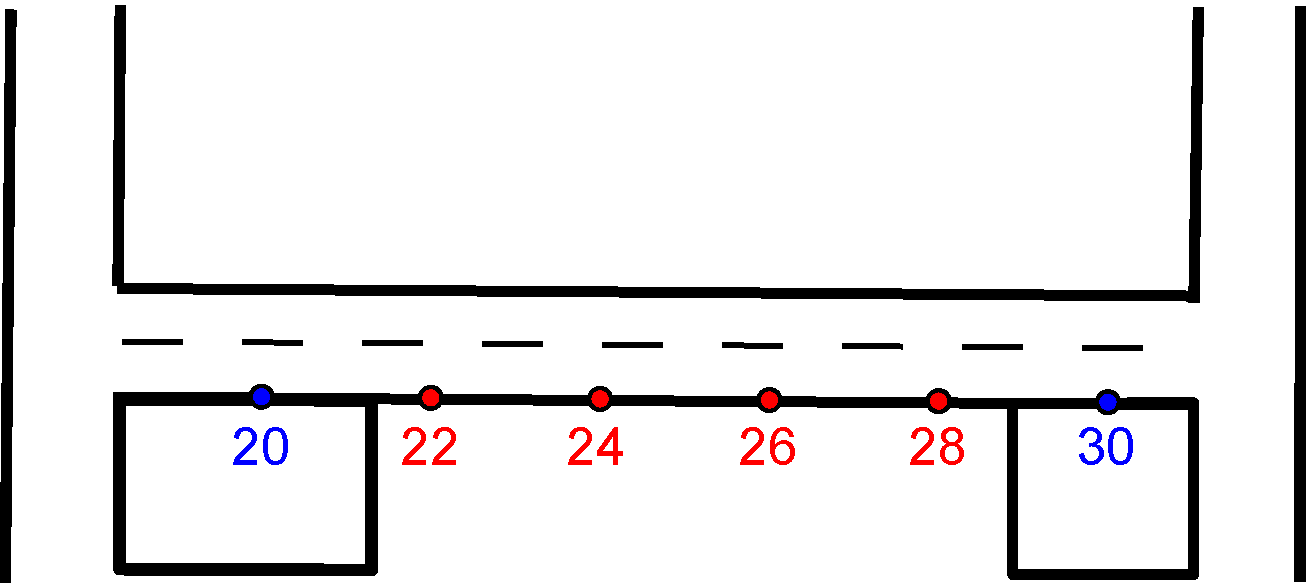
\includegraphics[width=.65\textwidth]{Fuentes_datos/Geocodificacion.pdf}
\caption{\small Interpolaci�n de direcciones. En azul, direcciones conocidas. En rojo, direcciones interpoladas.}
\label{Fig:Geocodificacion} 
\end{figure}

Esta pr�ctica, no obstante, no es del todo precisa, ya que asume que los edificios se encuentran equiespaciados, y por tanto son del mismo tama�o todos ellos, lo cual no sucede en la pr�ctica.  Adem�s de ello, el proceso presenta otras consideraciones particulares, tales como el hecho de que no en todos los pa�ses se sigue un mismo sistema de asignaci�n de direcciones postales, teniendo cada uno el suyo propio, que puede diferir en mayor o menor medida de lo que podr�a considerarse un sistema est�ndar. El supuesto habitual en que las direcciones pares se sit�an a un lado de la calle y las impares al lado contrario no resulta siempre cierto.

Otro aspecto a tener en cuenta es que el edificio se�alado con una direcci�n dada se identifica con una coordenada puntual, pero realmente ocupa una superficie \cite{WikipediaGeocoding}. Si esta es grande, puede presentar incluso varios puntos de acceso al mismo (o incluso accesos por varias calles distintas), con lo que la informaci�n que se recoge al geocodificar dicho edificio puede ser imprecisa e insuficiente.

Por todo ello, la interpolaci�n de direcciones permite una aproximaci�n v�lida para muchos usos, pero en aquellos casos en los que se requiera m�s precisi�n no pueden emplearse estas direcciones con total seguridad, ya que la exactitud de las coordenadas asociadas por el proceso de interpolaci�n puede variar notablemente seg�n sea la propia configuraci�n de los distintos edificios.

\subsection{Fotogrametr�a}
\label{Fotogrametria}

\index{Fotogrametr�a}

Un caso particular de digitalizaci�n lo encontramos en la \emph{fotogrametr�a}. En la definici�n cl�sica de \cite{Bonneval1972Eyrolles}, esta se define como la t�cnica para estudiar y definir con precisi�n la forma, dimensiones y posici�n en el espacio de un objeto cualquiera, utilizando medidas realizadas sobre una o varias fotograf�as. Esta definici�n no limita el alcance de la fotogrametr�a al �mbito de lo geogr�fico, y se utilizan sus principios en campos tales como la arqueolog�a o la documentaci�n de obras y monumentos, empleando para ello fotograf�as no a�reas, sino terrestres. Es la denominada \emph{fotogrametr�a terrestre}. No obstante, la rama de inter�s para este libro es la de la \emph{fotogrametr�a a�rea}, cuya base de trabajo tradicional son las fotograf�as a�reas.

Esta clase de fotogrametr�a viene, pues, ligada �ntimamente a los inicios de la teledetecci�n, cuando los sensores modernos que hemos estudiado antes en este mismo cap�tulo no se hab�an desarrollado, y los existentes (b�sicamente c�maras fotogr�ficas especialmente adaptadas a la toma de fotograf�as de tipo cartogr�fico) se montaban a bordo de aviones. Es por esta raz�n que tradicionalmente existe una conexi�n indudable entre ambas materias, no existiendo una frontera clara entre ambas, y se consideran en ocasiones como t�rminos id�nticos que hacen referencia la disciplina global de obtenci�n de im�genes y tratamiento de estas.

Hist�ricamente, el t�rmino \emph{teledetecci�n} aparece con posterioridad, una vez que las t�cnicas de toma de im�genes avanzan y dan un gran salto cualitativo con la aparici�n de las im�genes satelitales y los sensores electro--�pticos que ya conocemos. Algunos autores engloban la fotogrametr�a dentro de la teledetecci�n, mientras que otros se refieren con el termino teledetecci�n a las tecnolog�as m�s actuales y las consideran disciplinas distintas aunque muy relacionadas. Junto con la fotogrametria a�rea aparece la fotogrametr�a espacial, encargada de operar sobre im�genes de sat�lite bajo unos principios similares.

Dentro de este libro entenderemos por teledetecci�n todo el conjunto de t�cnicas y operaciones de obtenci�n de im�genes (que ya conocemos), as� como las de tratamiento y posterior extracci�n de resultados a partir de estas (que iremos viendo en otros cap�tulos), obteni�ndose estos resultados sin necesidad de establecer contactos con los objetos a estudiar, como corresponde a la definici�n dada en el apartado correspondiente. Dentro de ese conjunto de operaciones que nos llevan desde las im�genes a los resultados, entendemos como parte de la fotogrametr�a aquellas que tienen relaci�n con la acepci�n original del t�rmino, es decir, aquellas que derivan de la medici�n de elementos.

La denominaci�n, no obstante, no es tan relevante, y s� lo es sin embargo comprender la importancia de ambas, particularmente dentro de este cap�tulo como t�cnicas de producci�n cartogr�fica. 

En lo que respecta a la fotogrametr�a, el proceso de \emph{restituci�n} es el que interesa principalmente para el contenido de este cap�tulo, pues ofrece como resultado nuevas capas de datos tanto bidimensionales como, especialmente, tridimensionales. As�, pueden obtenerse tanto las capas vectoriales digitalizadas que ve�amos por ejemplo en el apartado \ref{Digitalizacion_manual}, como directamente Modelos Digitales de Elevaciones a partir de im�genes.\index{Restituci�n}

En realidad, los procesos de digitalizaci�n que ya hemos visto son tambi�n parte de la fotogrametr�a digital, y es habitual encontrarlos en los textos al uso sobre esta. Tambi�n lo son los procesos de rectificaci�n que se han citado en su momento, y que analizaremos en detalle m�s adelante en el cap�tulo \ref{Procesado_imagenes}. Como puedes ver, todas las t�cnicas est�n sumamente relacionadas, y las divisiones que hacemos pueden ser unas u otras en funci�n del enfoque que se d� para su estudio

Todas estas operaciones se llevan a cabo con una \emph{estaci�n fotogram�trica}, que comprende las herramientas necesarias para llevar estas a cabo (algunas, como los esc�neres, ya las conocemos). En funci�n del tipo de herramientas y t�cnicas distinguimos los siguientes tipos de fotogrametr�a, que representan a su vez la evoluci�n de la disciplina.\index{Estaci�n fotogram�trica}

\begin{itemize}
	\item Fotogrametr�a \textbf{anal�gica}. Basada en mediciones y procedimientos sobre im�genes anal�gicas
	\item Fotogrametr�a \textbf{anal�tica}. Basada en formulaciones matem�ticas y t�cnicas computacionales, permite obtener grandes precisiones.
	\item Fotogrametr�a \textbf{digital}. Basada en el trabajo con im�genes digitales dentro de un entorno computerizado.
\end{itemize}

El inter�s principal desde el punto de vista de los SIG es en la fotogrametr�a digital, ya que existe una gran relaci�n entre estos y las aplicaciones empleadas en dicho tipo de fotogrametr�a. Es en esta en la que pueden englobarse los procesos de digitalizaci�n que ya hemos visto, y no en las restantes formas m�s antiguas de fotogrametr�a. En la fotogrametr�a digital, la estaci�n fotogram�trica se articula sobre un ordenador en el cual se llevan a cabo los distintos procesos, no existiendo operaciones externas al mismo. As�, las im�genes se manejan dentro del ordenador y se visualizan a trav�s de �l, y la generaci�n de nueva cartograf�a tambi�n se produce de forma digital.

Esto no es muy diferente de lo que ve�amos en el caso de la digitalizaci�n en pantalla algunas paginas atr�s, pero el trabajo fotogram�trico engloba otros procesos adem�s de los que ya hemos visto. Uno de ellos es la generaci�n directa de cartograf�a de elevaciones, para la cual se requiere que el equipo empleado disponga de algunos elementos adicionales. Es decir, la estaci�n fotogram�trica digital es m�s compleja que un simple ordenador, un dispositivo de marcado (un rat�n) y un SIG, que eran los requisitos b�sicos para digitalizar en pantalla una imagen.

Una estaci�n fotogram�trica digital ha de tener, por ejemplo, capacidad para generar visualizaciones con sensaci�n de profundidad a partir de pares de im�genes, que son las que permiten la posterior digitalizaci�n de los elementos con sus elevaciones correspondientes. Los principios en los que se basan este tipo de visualizaciones son los mismos empleados en la fotogrametr�a no digital, fundamentados en la visi�n estereosc�pica. \index{Par estereosc�pico}

La visi�n tridimensional en el ser humano se basa en el hecho de que la imagen que ve cada ojo es ligeramente distinta a la del otro, lo cual permite al cerebro extraer informaci�n volum�trica y generar una verdadera visi�n tridimensional. En el caso de la fotogrametr�a, si en lugar de utilizar una �nica imagen a�rea o de sat�lite empleamos dos, cada una de ellas tomada desde un punto distinto, resulta posible recrear el efecto que ambas im�genes tendr�an para la reconstrucci�n tridimensional de la escena, y <<enga�ar>> al cerebro del observador para que este pueda observar la escena con volumen y profundidad.

Cuando se emplean im�genes de sat�lite, los pares se pueden obtener con aquellas plataformas y sensores que permiten variar el �ngulo de visi�n, de modo que en la misma pasada del sat�lite se toman im�genes de una zona desde distintos puntos. El sensor toma una imagen cenital y posteriormente, una vez ha superado la zona en su recorrido, toma una segunda imagen mirando <<hacia atr�s>>, la cual, combinada con la primera, permite el levantamiento del terreno y la realizaci�n de los procesos fotogram�tricos (Figura \ref{Fig:Par_estereo_satelite}).

\begin{figure}[!hbt]
\centering
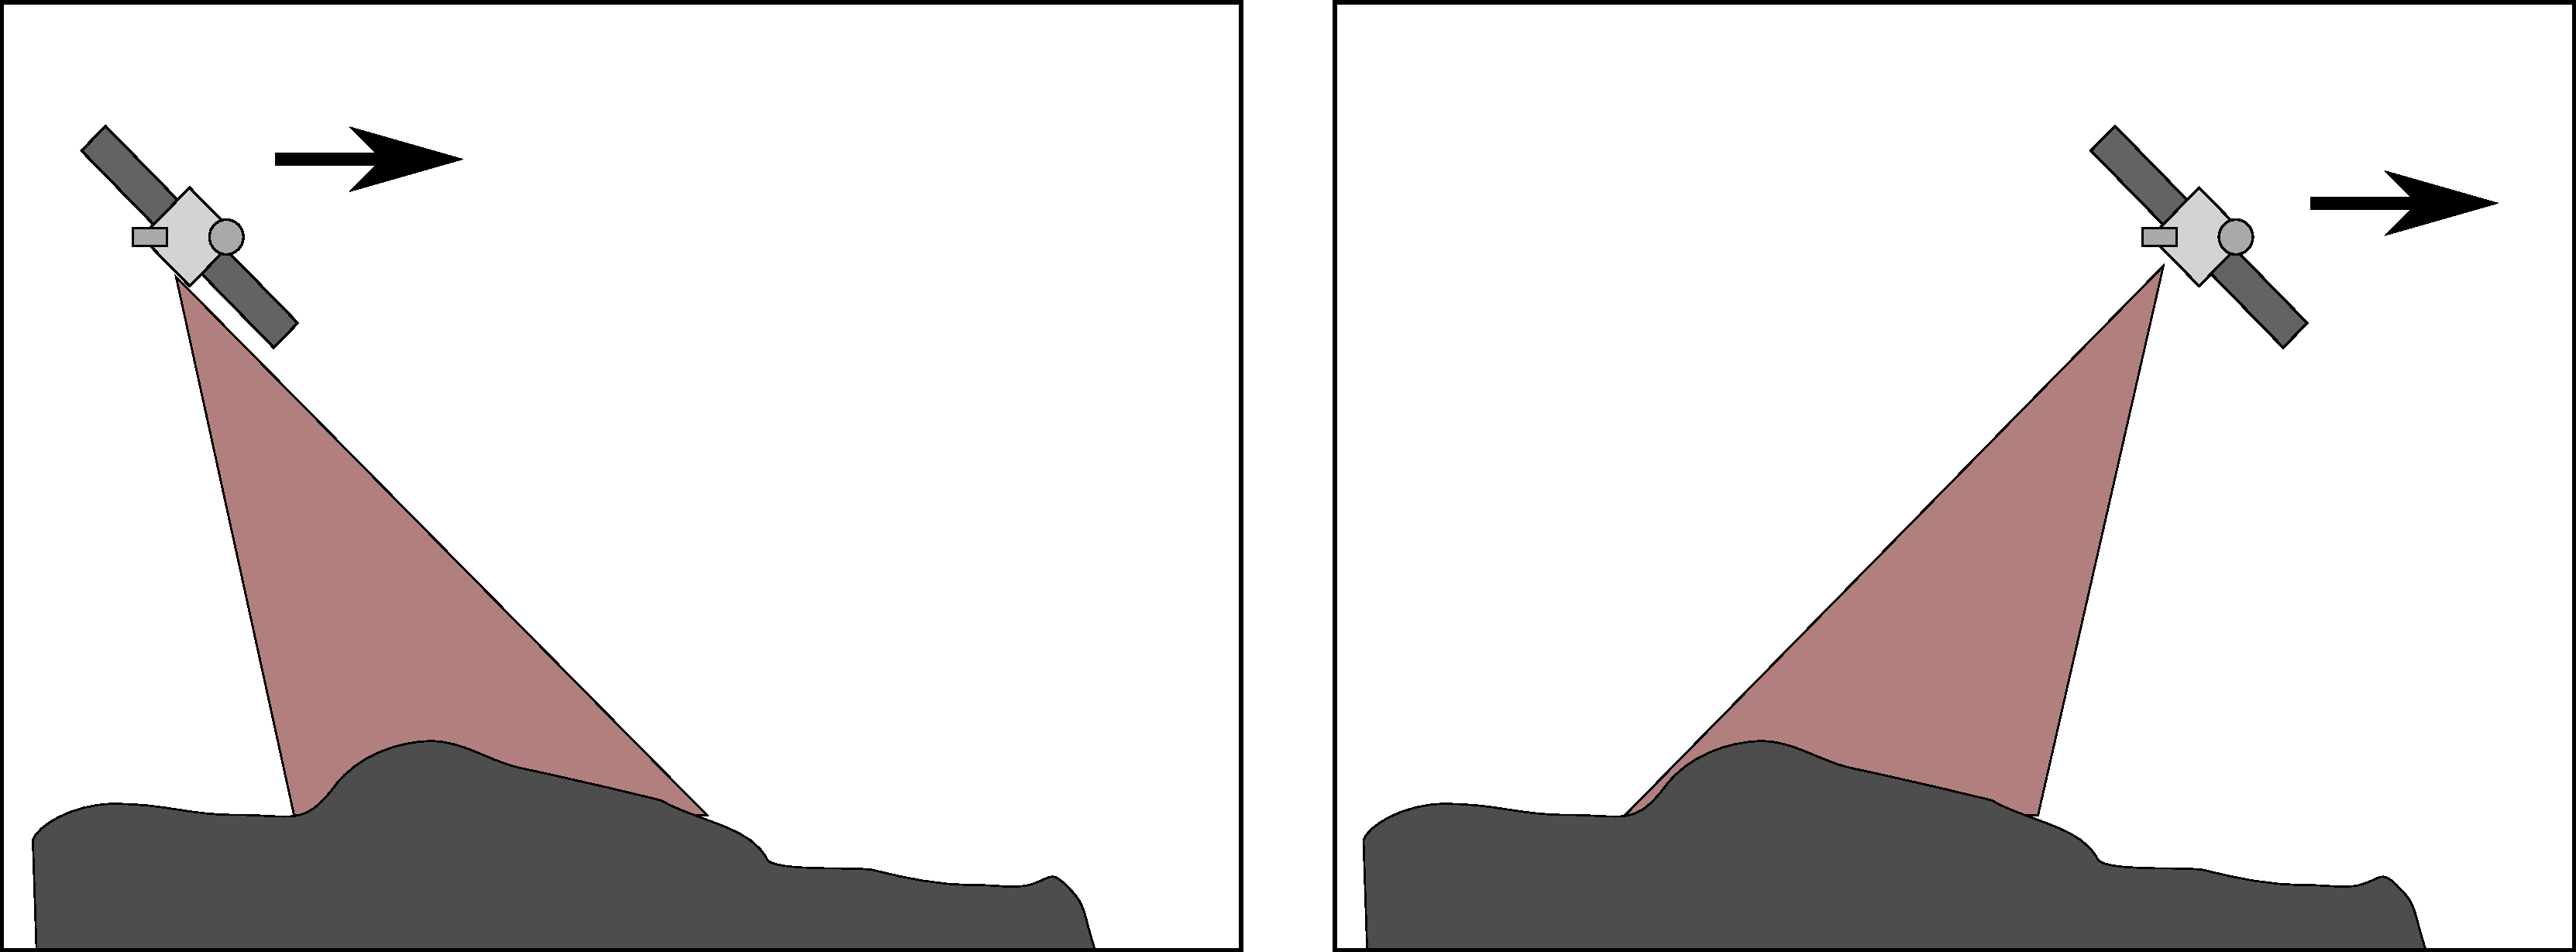
\includegraphics[width=.85\textwidth]{Fuentes_datos/Par_estereo_satelite.pdf}
\caption{\small Toma de pares de im�genes estereos�picas desde un sat�lite, mediante variaci�n del �ngulo de visi�n.}
\label{Fig:Par_estereo_satelite} 
\end{figure}

El sensor HRS que montan los sat�lites SPOT, o el sensor ASTER, ambos son capaces de tomar este tipo de im�genes. En la direcci�n Web \cite{webSPOTDEM} puede encontrarse informaci�n detallada sobre las cartograf�a de elevaciones generada a partir de pares de im�genes tomadas por el sat�lite SPOT, junto con algunas ilustraciones y animaciones explicativas al respecto. \index{SPOT}\index{ASTER}

Las formas de conseguir que el observador perciba la profundidad de la escena a partir de las im�genes son variadas, y van desde el uso de sencillos instrumentos �pticos o la generaci�n de anaglifos (im�genes que combinan la informaci�n del par estereosc�pico y que se han de observar con gafas con filtros distintos para cada ojo), hasta otras t�cnicas m�s complejas y elaboradas. En la fotogrametr�a no digital, el empleo de restituidores anal�ticos %como el mostrado en la figura \ref{Fig:Restituidor_analitico} 
ha sido la metodolog�a habitual. En la fotogrametr�a digital, este puede sustituirse por un equipo con dos monitores, cada uno de los cuales muestra una de las im�genes del par, y se emplean gafas especiales que son las encargadas de generar en el observador la sensaci�n de profundidad .\index{Anaglifos}

\begin{figure}
\centering
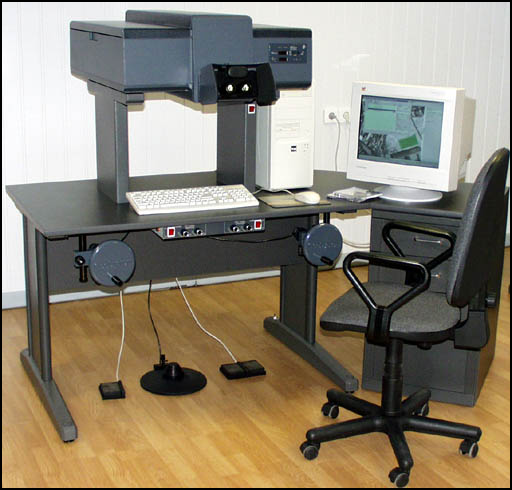
\includegraphics[width=.5\textwidth]{Fuentes_datos/Estacion_fotogrametrica_digital.png}
\caption{\small Estaci�n fotogram�trica digital.}
\label{Fig:Estacion_fotogrametrica_digital} 
\end{figure}

Adem�s de lo anterior, la estaci�n fotogram�trica digital dispone de perif�ricos espec�ficos tales como ratones 3D, o manivelas como las que presentan los restituidores anal�ticos, facilitando as� la adaptaci�n de los operarios a este tipo de estaci�n (Figura \ref{Fig:Estacion_fotogrametrica_digital}).

Por �ltimo el software que implementan, y que es el encargado de representar las im�genes y acoger el proceso de digitalizaci�n, suele ser espec�fico, y es frecuente que se distribuya como parte de toda una estaci�n fotogram�trica compuesta por los elementos rese�ados anteriormente. Algunos SIG incorporan progresivamente capacidades adaptadas de este tipo de programas, pero por el momento la labor fotogram�trica queda reservada para este tipo de aplicaciones espec�ficas, siendo el SIG tan solo un beneficiario directo de sus productos.

Para el lector interesado en saber m�s acerca de los distintos elementos de la fotogrametr�a, obras como  \cite{Lerma2002UPV} o \cite{Brito2002IME} son recomendables, esta �ltima disponible de forma libre. En la direcci�n Web \cite{webFotogrametriaUNEX} puede encontrarse otra excelente referencia libre en dos tomos sobre fotogrametr�a anal�tica y digital.

\subsection{Calidad de la digitalizaci�n}
\label{Condiciones_digitalizacion}

\index{Digitalizaci�n!calidad}

Uno de los aspectos m�s importantes del proceso de digitalizaci�n es la calidad del resultado obtenido, que debe tratar de ser lo m�s cercano posible a la calidad original de la informaci�n que se digitaliza, es decir, del mapa o imagen original. Independientemente de la precisi�n del equipo utilizado o la habilidad y experiencia del operario, la digitalizaci�n no es por completo perfecta, conteniendo siempre ciertas deficiencias y errores. 

Adem�s de los errores que puedan incorporarse en las distintas fases del proceso de digitalizaci�n (sea este del tipo que sea), hay que considerar que las fuentes originales a digitalizar tambi�n pueden incluir los suyos propios. As�, el proceso de escaneado puede incorporar distorsiones geom�tricas, pero es posible que el mapa o fotograf�a a�rea de partida tambi�n presente alguna distorsi�n como consecuencia de su deterioro, m�s patente cuanto m�s antigua sea esta. 

La informaci�n contenida en el documento cartogr�fico puede tambi�n contener elementos problem�ticos de cara a obtener un producto de calidad, que pueden ir desde l�neas borradas total o parcialmente a manchas en el propio mapa derivadas de su uso habitual \cite{Heywood1998Longman}.

Dentro de los errores que aparecen como consecuencia de la digitalizaci�n en s�, un tipo importante de ellos son las discrepancias y coincidencias imperfectas entre las distintas entidades, tal como las que se muestran en la figura \ref{Fig:Imprecisiones_digitalizacion}

\begin{figure}[!hbt]   
\centering
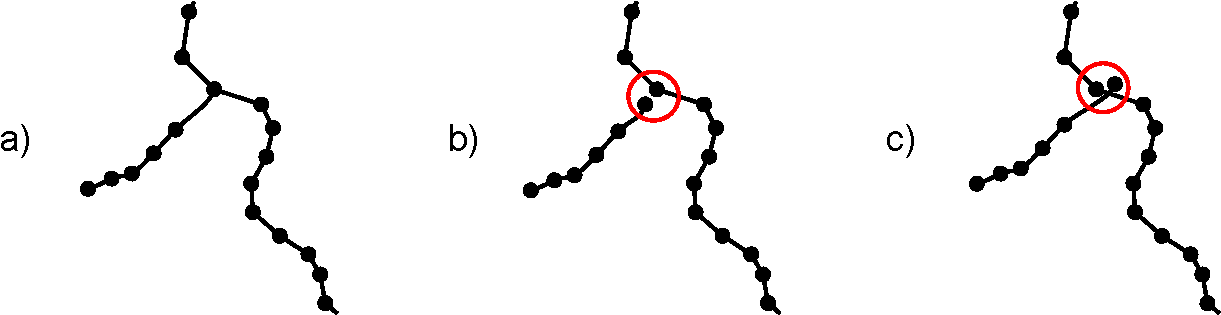
\includegraphics[width=.8\textwidth]{Fuentes_datos/Imprecisiones_digitalizacion.pdf}
\caption{\small Errores derivados del proceso de digitalizaci�n. a) Versi�n correcta, con nodos coincidentes. b) y c) Versiones con errores que causan una falsa desconexi�n entre las l�neas.}
\label{Fig:Imprecisiones_digitalizacion} 
\end{figure}

Estas imprecisiones son causantes de numerosos problemas, tales como la aparici�n de pol�gonos esp�reos en las operaciones de solape entre capas vectoriales, que veremos en el cap�tulo \ref{Operaciones_geometricas}.\index{Pol�gono!espureo}

Debido a esto, las capacidades de edici�n de los SIG incorporan funcionalidades que permiten evitar estos errores en el momento de la digitalizaci�n, ayudando al operario en su tarea y permiti�ndole alcanzar una exactitud y precisi�n imposible de lograr sin estas funcionalidades. Entre ellas, es especialmente importante el establecimiento de tolerancias y ajuste autom�tico en funci�n de ellas (esto se conoce con el t�rmino ingles \emph{snapping}), que ayudan a garantizar la coincidencia entre los distintos v�rtices. \index{Snapping}

De este modo, pol�gonos adyacentes o lineas que se cortan en un punto dado lo hacen con total exactitud. Dichos pol�gonos comparten exactamente el mismo lado con las mismas coordenadas exactas, o se cruzan en el mismo e id�ntico punto, y no �nicamente pasan por un punto cercano (pero distinto) definido con la precisi�n con la que el operador haya podido ajustar ambas entidades visualmente. La coincidencia no es solo visual, sino num�rica. La figura \ref{Fig:Snapping} muestra un ejemplo de la utilizaci�n de \emph{snapping} en un proceso de digitalizaci�n.

\begin{figure}
\centering
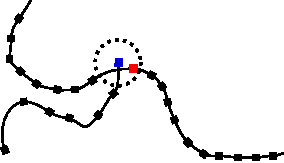
\includegraphics[width=.4\textwidth]{Fuentes_datos/Snapping.pdf}
\caption{\small Ajuste autom�tico mediante tolerancia(\emph{snapping}). El nodo azul representa el nodo en edici�n. La tolerancia de enlace queda marcada por el circulo punteado. Puesto que el nodo rojo de la l�nea preexistente se encuentra dentro de esa tolerancia, al a�adir el nuevo nodo (azul), este autom�ticamente se situar� en las coordenadas del nodo rojo, garantiz�ndose as� la coincidencia.}
\label{Fig:Snapping} 
\end{figure}

Mediante estas funcionalidades, el operador simplemente selecciona un punto, y el sistema digitalizador lo desplaza para que coincida con el punto existente m�s cercano, siempre que se encuentre a menos distancia que la tolerancia establecida de antemano.

El hecho de que exista una completa coincidencia es especialmente importante cuando la capa vectorial que se digitaliza contiene informaci�n topol�gica. La topolog�a exige que la coincidencia sea correcta y defina perfectamente la relaci�n entre las entidades. Para los ejemplos b) y c) de la figura \ref{Fig:Imprecisiones_digitalizacion}, las l�neas no est�n conectadas ya que no existe coincidencia en el nodo. Si los puntos est�n suficientemente cercanos, puede <<parecer>> que son coincidentes, pero el SIG no los detectar� como tales y no se podr� llevar a cabo ning�n an�lisis topol�gico con esas l�neas (por ejemplo, suponiendo que representan v�as de comunicaci�n y se quiere hacer un an�lisis de redes con ellas).

La digitalizaci�n de entidades en caso de querer recoger la topolog�a\index{Topolog�a} de las mismas debe obedecer una serie de reglas, a saber\cite{GrassDigitizing}:

\begin{itemize}
	\item Las l�neas deben cruzarse en nodos, en caso de que exista relaci�n (conexi�n) entre ellas.
	\item Las lineas que coinciden en un nodo com�n deben coincidir exactamente. Las funciones de \emph{snapping} se han de utilizar por ello durante la digitalizaci�n.
	\item Los lados comunes de los pol�gonos deben digitalizarse una �nica vez.
	\item Las �reas deben ser cerradas (el primer punto ha de coincidir exactamente con el �ltimo). Las funciones de \emph{snapping} o el cierre autom�tico de l�neas (asignar sistem�ticamente al �ltimo punto del contorno del pol�gono las coordenadas del primero) deben emplearse para ello.
\end{itemize}

Todos aspectos relativos a la calidad de datos, entre los cuales se incluyen las aspectos relativos a los errores del proceso de digitalizaci�n, se tratan con mayor profundidad en el cap�tulo \ref{Calidad_datos}.\index{Datos!calidad}


\section{GPS}
\label{GPS}

Uno de los hitos en la aparici�n de nuevas fuentes de datos geogr�ficos es la aparici�n de los \emph{Sistemas Globales de Navegaci�n por Sat�lite} (GNSS)\footnote{\emph{Global Navigation Satellite System}}, que permiten la obtenci�n de coordenadas geogr�ficas de un modo inmediato, con las consecuencias que esto tiene para su uso en actividades como la elaboraci�n de cartograf�a.\index{GNSS}\index{GPS}

En esencia, un GNSS es un sistema que permite conocer en todo momento y en cualquier punto del globo la localizaci�n exacta de dicho punto con un margen de error del orden de unos pocos metros o menos. Para ello, se basan en el env�o de se�ales entre un dispositivo situado en el punto concreto y una red de sat�lites, pudiendo establecerse la posici�n exacta mediante las caracter�sticas de dicha transmisi�n.

El ejemplo m�s extendido de un GNSS es el Sistema de Posicionamiento Global (Global Positioning System, o GPS)\footnote{El nombre completo del sistema es NAVSTAR--GPS (NAVigation SysTem And Ranging - Global Position System)}, originalmente puesto en funcionamiento por el Departamento de Defensa de los Estados Unidos. Actualmente, este es el �nico GNSS completamente operativo, aunque existen otros tales como el GLONASS ruso, el COMPASS chino o el \emph{Galileo} europeo, cuyo funcionamiento completo est� previsto a corto plazo. \index{GLONASS}\index{Galileo}\index{COMPASS}

\subsection{Fundamentos del sistema GPS}

El sistema GPS se divide en tres subsistemas o \emph{segmentos}:

\begin{itemize}
	\item \textbf{Segmento espacial}. Lo componen los sat�lites de la constelaci�n GPS (un total de 27, siendo 24 de ellos operativos y 3 de reserva), con los cuales se comunican las unidades receptoras, y en funci�n de los cuales puede triangularse la posici�n actual de estas.
	\item \textbf{Segmento de control}. Lo forman un conjunto de estaciones terrestres que controlan el funcionamiento de los sat�lites, pudiendo enviar se�ales a estos para modificar su comportamiento.
	\item \textbf{Segmento de usuarios}. Lo conforman los receptores GPS y todos los dispositivos que hacen uso de la se�al de los sat�lites para el c�lculo de posiciones.
\end{itemize}

\index{Segmentos!del sistema GPS}

Los sat�lites del segmento espacial emiten una se�al compleja cuyo contenido puede dividirse esencialmente en dos bloques de informaci�n:

\begin{itemize}
	\item \textbf{Se�ales empleadas para el c�lculo de distancias}. Estas incluyen dos c�digos: P(Precise) y C/A (Coarse/Aquisition). El segundo de ellos es el empleado habitualmente, ya que el primero se encuentra encriptado y est� pensado para uso militar, mientras que el C/A esta disponible para todos los usuarios.
	\item \textbf{Mensajes de navegaci�n}. Estos informan de la posici�n orbital del sat�lite (conocida como \emph{efem�ride}), y pueden asimismo contener informaci�n adicional referente al segmento espacial.
\end{itemize}

\index{Efem�ride}

Las se�ales para el c�lculo de distancias (en la terminolog�a GPS estas distancias se conocen como \emph{pseudodistancias}) se env�an mediante una onda portadora conocida como L1, correspondiente a una frecuencia de 1575,42 MHz . El c�digo P se env�a adem�s en una segunda portadora denominada L2, con una frecuencia de 1227,60 MHz.\index{Pseudodistancias}

El funcionamiento del sistema se basa en la triangulaci�n de la posici�n mediante las se�ales procedentes de un cierto n�mero de los sat�lites. Esta posici�n se calcula no �nicamente en sus coordenadas \emph{x} e \emph{y}, sino tambi�n en \emph{z}, es decir en elevaci�n. El sistema GPS emplea como sistema geod�sico de referencia el WGS84 \cite{WGS84}. La precisi�n en el c�lculo de la elevaci�n es menor que la correspondiente a las restantes coordenadas, aunque tambi�n es de utilidad y puede emplearse en aplicaciones que van desde levantamientos y replanteos a usos en tiempo real como el c�lculo de elevaci�n en vuelos \cite{Graas1991Navigation}.\index{WGS84}

La posici�n de los sat�lites es conocida en todo momento, y los propios sat�lites informan de ella a los receptores a trav�s de los mensajes de navegaci�n. En base a esas posiciones orbitales, el proceso de triangulaci�n que se lleva a cabo en el sistema GPS no se basa en el trabajo con �ngulos, sino con distancias.

El c�lculo de la distancia puede realizarse utilizando la informaci�n de las se�ales (los c�digos C/A o P), o bien empleando las propias portadoras. El primer m�todo es m�s sencillo y r�pido, ya que no es necesario que el receptor <<escuche>> la se�al durante un periodo prolongado de tiempo, lo cual s� es necesario en el segundo, como a continuaci�n veremos. 

En el caso de emplear la portadora, se mide el desfase entre esta y una se�al generada por el receptor, lo cual permite calcular una parte de la distancia (la que es menor que la longitud de onda de la se�al). La distancia total es igual a esta parte calculada m�s un numero entero de veces la longitud de onda. El valor de este numero entero es, no obstante, desconocido. Su c�lculo se conoce como \emph{resoluci�n de la ambig�edad} (AR), y requiere escuchar la se�al del sat�lite durante un cierto tiempo para recopilar datos suficientes que permitan el c�lculo del valor antedicho.\index{Resoluci�n!de la ambig�edad}

As�, la resoluci�n de la ambig�edad es la que hace necesario un tiempo de \emph{inicializaci�n} de la unidad, con objeto de conocer esa constante en el desfase. Si la unidad pierde contacto con el sat�lite, es necesario de nuevo proceder a la resoluci�n de las ambig�edades, quedando el receptor inoperativo durante ese periodo de tiempo. M�s detalles sobre la resoluci�n de la ambig�edad en el sistema GPS puede encontrarse en \cite{Torrecillas1998Mapping}.

Puesto que la velocidad a la que la se�al se desplaza es muy elevada, se requieren relojes muy precisos para poder medir con precisi�n los tiempos tan cortos que tarda dicha se�al en recorrer la distancia entre sat�lite y receptor. A bordo de los sat�lites se montan relojes at�micos de muy alta precisi�n, pero las unidades receptoras no disponen de relojes tan precisos. Es por este motivo que, como veremos, han de introducirse correcciones y c�lculos adicionales con el fin de obtener mayores precisiones en la medida del tiempo.

Si el receptor es capaz de establecer comunicaci�n con tres sat�lites, dispone ya de informaci�n suficiente para conocer su posici�n $(x,y)$ como intersecci�n de las esferas centradas en cada uno de dichos sat�lites y con radio la distancia existente entre este y el receptor. Con cuatro sat�lites se puede ya obtener la posici�n $(x,y,z)$.

Un n�mero mayor de sat�lites (cuatro al menos) es necesario, no obstante, para eliminar las imprecisiones debidas a los distintos elementos implicados, y se emplean habitualmente modelos m�s complejos que utilizan los datos de m�ltiples sat�lites y efect�an correcciones en funci�n de ellos. Las deficiencias de los relojes que emplean los receptores pueden corregirse mediante la utilizaci�n de nuevos sat�lites, que permiten calcular con exactitud el tiempo, variable de gran importancia en el proceso y sin la cual no se pueden obtener precisiones elevadas.

Los receptores actuales est�n preparados para trabajar con un n�mero m�ximo de sat�lites habitualmente igual a 12, por lo que en todas circunstancias el receptor trata de localizar siempre el mayor n�mero posible de sat�lites con objeto de lograr una mayor precisi�n.

El dise�o de la red de sat�lites est� pensado para garantizar que en cualquier punto de la superficie terrestre y en cualquier momento, un receptor puede localizar el n�mero necesario de sat�lites para obtener con exactitud su precisi�n. La localizaci�n en la que se disponen los sat�lites con los que se establece comunicaci�n no es irrelevante, ya que condiciona la precisi�n del posicionamiento, afectando a lo que se conoce como \emph{diluci�n de la precisi�n} (DOP\footnote{Dilution of Precision}). Si los �ngulos de los sat�lites son grandes, la precisi�n que se obtiene es mayor que si estos son menores (Figura \ref{Fig:DOP}).\index{Dilution of Precision}

\begin{figure}
\centering
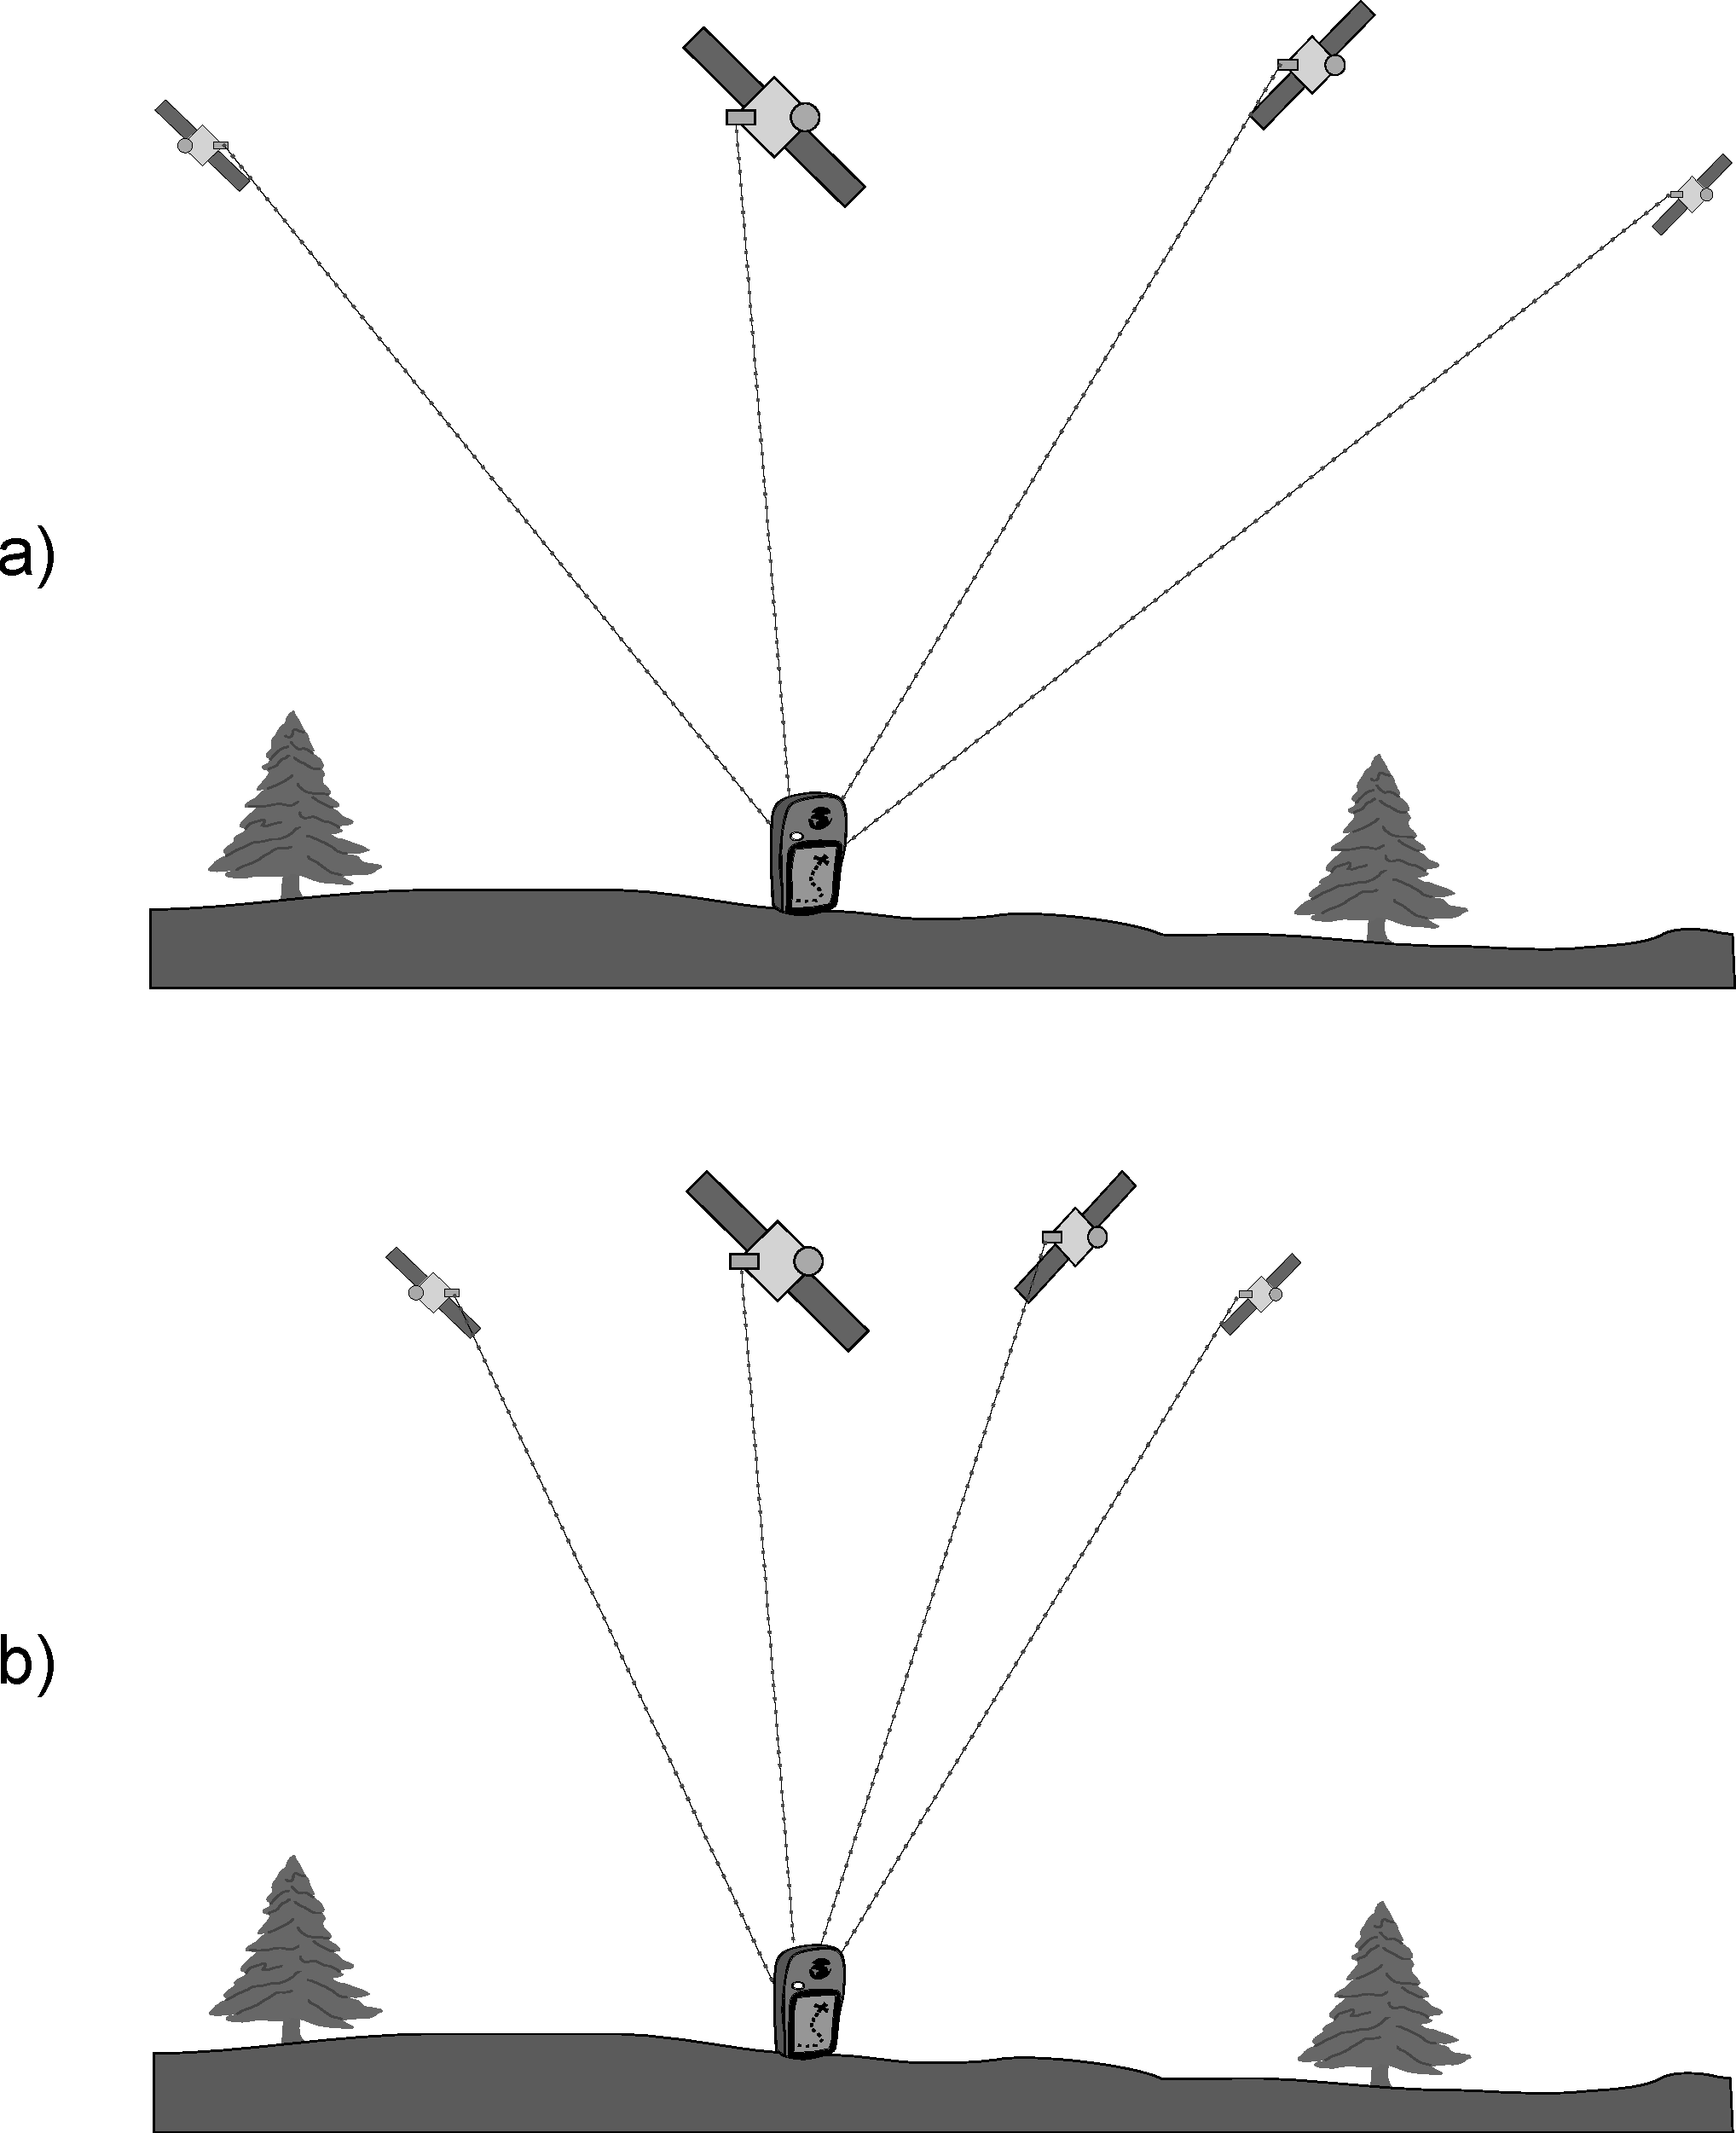
\includegraphics[width=.5\textwidth]{Fuentes_datos/DOP.pdf}
\caption{\small Diluci�n de la precisi�n. La geometr�a de los sat�lites en el ejemplo a) da una mayor precisi�n en el c�lculo de la posici�n del receptor que la del ejemplo b).}
\label{Fig:DOP} 
\end{figure}

Junto a esto, existen otras muchas fuentes de error en el sistema GPS, cada una de las cuales afecta a la precisi�n del mismo. Entre ellas, cabe destacar las siguientes:

\begin{itemize}
	\item Errores en la posici�n de los sat�lites.
	\item Errores por el rebote de la se�al en otros elementos tales como edificios, con anterioridad a alcanzar el receptor.
	\item Errores derivados del paso de la se�al por la atm�sfera. Al atravesar la ionosfera y la troposfera se genera un retraso por la alteraci�n que dicho paso produce sobre la se�al.
	\item Errores en la precisi�n de los relojes, ya mencionados.
	\item \emph{Disponibilidad selectiva}. Debido a su concepci�n como una herramienta militar, el departamento de Defensa de los Estados Unidos, propietario del sistema, introduc�a errores aleatorios en las se�ales, de tal forma que esta quedaba degradada y los usuarios civiles no pod�an obtener una precisi�n muy elevada. La disponibilidad selectiva fue eliminada en el a�o 2000.
\end{itemize}

\index{GPS!fuentes de error}

En conjunto, todos estos errores suman desviaciones apreciables, que sin embargo pueden corregirse con la aplicaci�n de t�cnicas adicionales, por ejemplo incorporando informaci�n adicional procedente de otros receptores. Una de estas t�cnicas es el denominado \emph{GPS diferencial}, pensado en origen para eliminar el error de la disponibilidad selectiva, aunque tambi�n eficaz para corregir una buena parte los restantes errores citados anteriormente.\index{GPS!diferencial}

Para la aplicaci�n del GPS diferencial se requiere no solo un receptor �nico (aquel del cual se quiere calcular su posici�n), sino tambi�n otro receptor fijo de referencia cuyas coordenadas se conocen con alta precisi�n. Este receptor fijo es, a su vez, un receptor de alta precisi�n y, adem�s de calcular su propia posici�n, emite informaci�n que las unidades receptoras pueden aprovechar para corregir sus mediciones. El receptor m�vil, l�gicamente, tiene que soportar este tipo de correcciones, para poder hacer uso de la se�al de la estaci�n de referencia.

Los datos que permiten llevar a cabo la correcci�n puede obtenerse en el receptor mediante radio, descargarse por Internet mediante una conexi�n inal�mbrica, o bien utilizar una constelaci�n de satelites adicional dedicada a elaborar y servir este tipo de datos.

La correcci�n puede realizarse fuera del propio receptor, a posteriori, utilizando software adecuado y los mismos datos de correcci�n que si se realiza la correcci�n en tiempo real.

El fundamento de este sistema es que los errores que afectan al receptor m�vil tambi�n afectan al de referencia. No obstante, la magnitud del error que afecta al receptor de referencia puede conocerse, ya que se conoce la coordenada exacta de este, y en base a eso puede eliminarse el error que afecta al receptor m�vil, asumiendo que ambos errores son de similar �ndole.

En la actualidad, aplicando estas t�cnicas de correcci�n diferencial, un GPS puede obtener precisiones del orden de 2 metros en latitud y longitud, y 3 en altitud\cite{wikipediaGPS}. Sin correcci�n diferencial, esta precisi�n es de unos 10--20 metros.

La figura \ref{Fig:DGPS} muestra un esquema del funcionamiento del GPS diferencial.

\begin{figure}
\centering
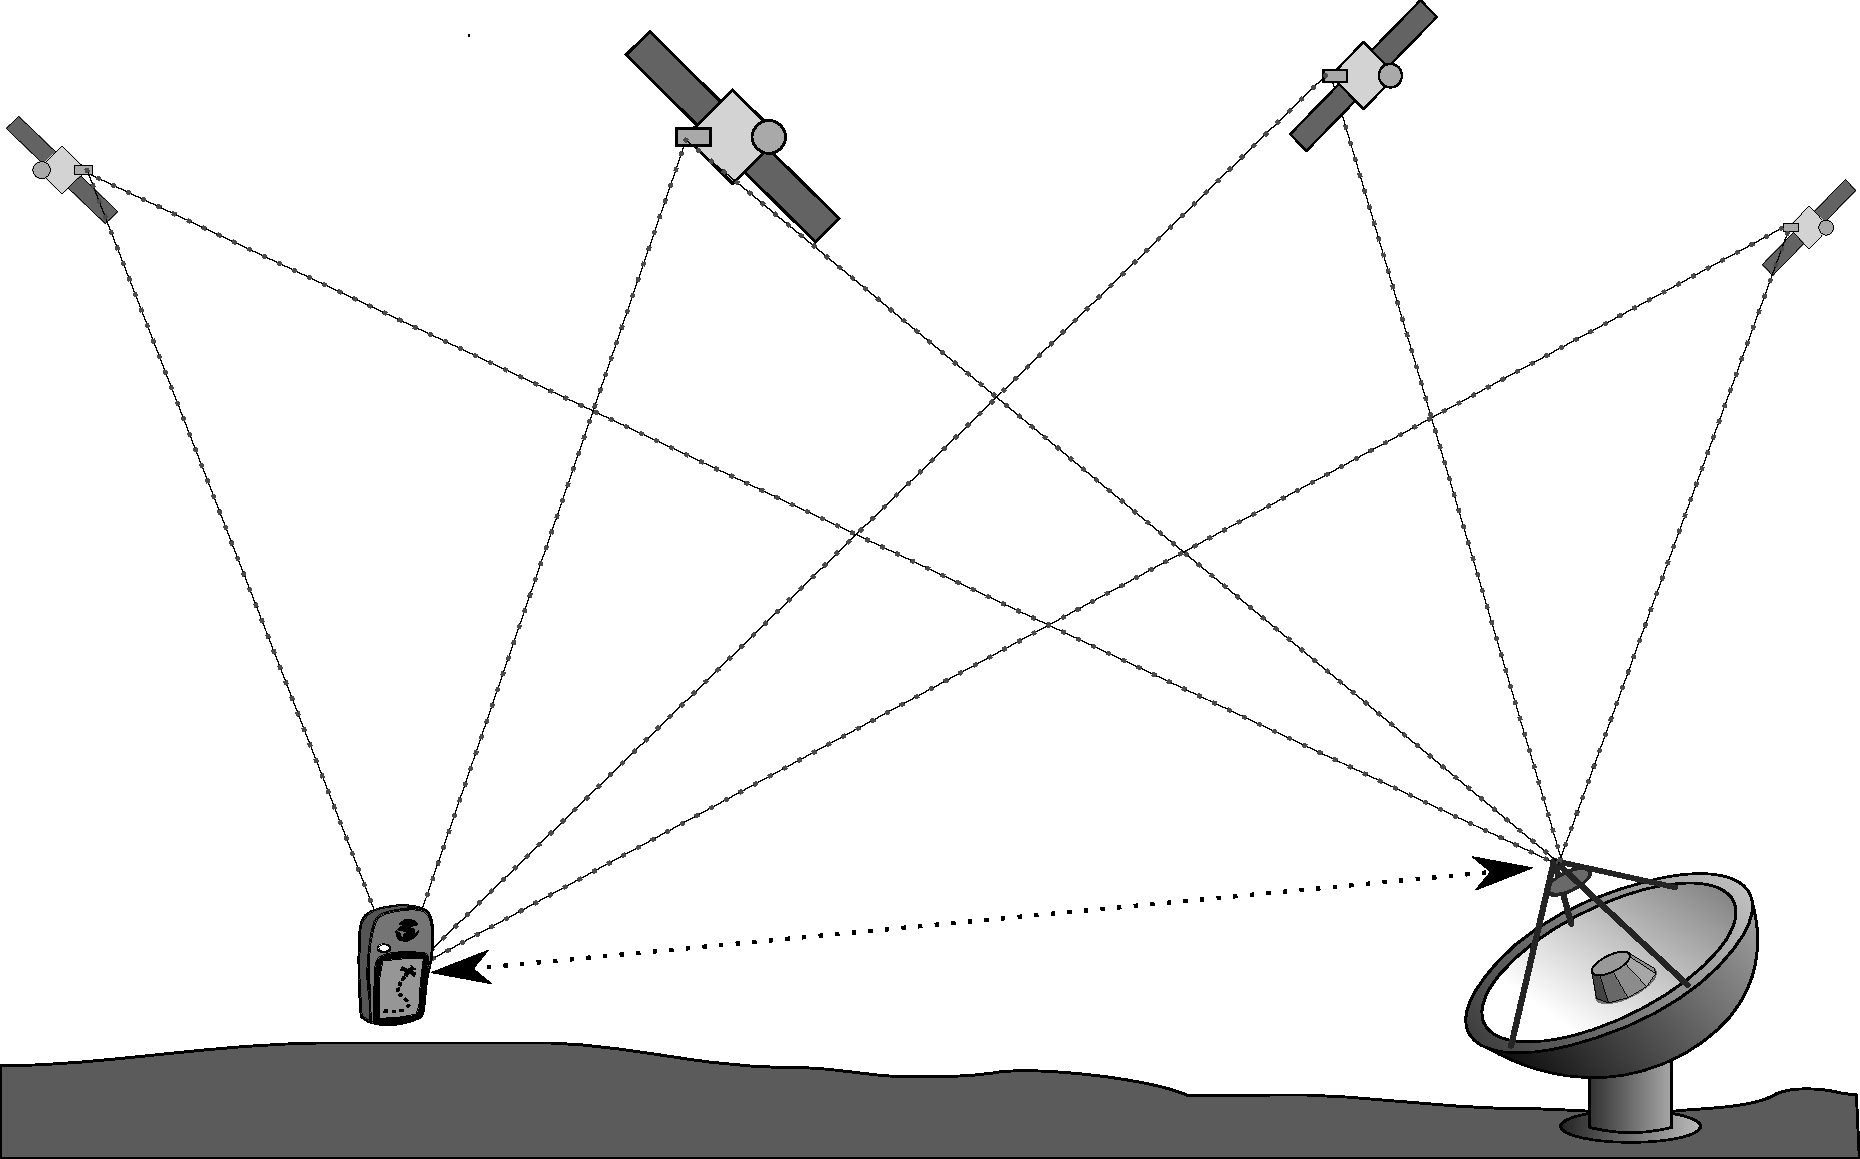
\includegraphics[width=.5\textwidth]{Fuentes_datos/DGPS.pdf}
\caption{\small Esquema de funcionamiento del GPS diferencial}
\label{Fig:DGPS} 
\end{figure}

Adem�s de la literatura abundante sobre GPS, los fabricantes de receptores GPS, muy populares hoy en d�a para numerosas actividades, ponen a disposici�n del p�blico una gran cantidad de informaci�n sobre sus productos y tambi�n sobre los fundamentos del sistema GPS. En ese sentido, una buena referencia es el sitio Web \cite{webTrimble}, donde puede encontrarse una descripci�n detallada de los distintos elementos del sistema GPS, acompa�ada de im�genes y animaciones sumamente did�cticas. En \cite{webHowWorkGPS} tambi�n puede encontrarse informaci�n de inter�s y f�cil acceso.


\subsection{Tipos de receptores}

La precisi�n del sistema global GPS depende del tipo de receptor GPS (o, en el lenguaje com�n, GPS a secas) que se emplee, obteni�ndose mayores precisiones con receptores m�s avanzados, siempre dentro de las posibilidades del propio sistema GPS.

En funci�n de sus caracter�sticas y de la forma en que operan, podemos distinguir los siguientes tipos de receptores GPS:

\begin{itemize}
	\item \textbf{Receptores secuenciales}. Establece conexiones secuenciales con los distintos sat�lites disponibles, estando conectado a uno o dos a lo sumo simult�neamente. Estos receptores son m�s econ�micos, ya que esta forma de operar requiere equipos menos complejos, aunque la precisi�n que se obtiene tambi�n es menor.
	\item \textbf{Receptores continuos}. Disponen de m�s canales de radio que los anteriores y ello permite que la conexi�n a los sat�lites sea continua, sin tener que alternar entre uno y otro. La precisi�n que se obtiene es mayor, pero se trata de equipos m�s caros.
	\item \textbf{Receptores con canales multiplexados}. El esquema de funcionamiento es similar al secuencial, alternando entre los distintos sat�lites y utilizando un �nico canal. No obstante, utilizan software m�s complejo y procesadores m�s potentes, de forma que esta alternancia se puede producir con una frecuencia mucho m�s elevada. 
\end{itemize}

\index{GPS!receptores}

A d�a de hoy, es habitual que incluso los GPS de menor coste tengan m�ltiples canales, permitiendo la conexi�n continua con un n�mero elevado de sat�lites.

Como hemos visto, las se�ales emitidas por los sat�lites contienen dos c�digos (C/A y P) que se transmiten modulados sobre dos ondas portadoras distintas (L1 y L2). No todos los receptores GPS son capaces de utilizar estos elementos de las se�ales, y en funci�n de ello podemos tambi�n clasificarlos. 

Los m�s sencillos �nicamente basan sus c�lculos en el c�digo C/A, mientras que los m�s avanzados y complejos son capaces de utilizar el c�digo P (encriptado, por lo que es necesaria una clave correspondiente), as� como las portadoras para un c�lculo m�s preciso, seg�n se explic� en un punto anterior.

Por �ltimo, y teniendo en cuenta que el sistema GPS mide las coordenadas $(x,y,z)$ y el tiempo, y que existen diferentes precisiones en funci�n de la tecnolog�a que los receptores utilicen, encontramos una gran variedad de unidades receptoras, seg�n estas se adapten para uno u otro uso principal. En l�neas muy generales, los siguientes son algunos de los tipos principales en funci�n de dicho uso.

\begin{itemize}
	\item GPS para uso general. Unidades peque�as y port�tiles, de bajo coste, para actividades al aire libre, donde no se requiere una precisi�n elevada sino simplemente un conocimiento de la posici�n aproximada. Se emplean, por ejemplo, para recoger rutas en senderismo o navegaci�n. Estas unidades, adem�s de informar de la posici�n y ser capaces de almacenar esta, suelen disponer de capacidades de representaci�n de mapas en pantalla, de forma que la informaci�n sobre la posici�n sea m�s �til para el usuario. Otros, como los navegadores GPS para coche, son capaces de calcular rutas �ptimas, combinando la posici�n calculada con una cartograf�a de v�as previamente incorporada al dispositivo.
		La figura \ref{Fig:gps_1}a muestra un receptor GPS de uso general.
	\item GPS para la medici�n topogr�fica. Unidades de medio tama�o, generalmente con una antena independiente que se conecta a la unidad y que el propio operario carga a la espalda. La antena garantiza mayor precisi�n y una mejor localizaci�n de sat�lites en condiciones tales como zonas bajo arbolado. Est�n pensados para un uso profesional en levantamientos o replanteos, ofreciendo buena precisi�n en todas las coordenadas. 
	En la figura \ref{Fig:gps_1}b puede verse unos de estos receptores.
	Estos son los GPS de mayor inter�s para el uso dentro de un SIG, ya que ofrecen datos de campo precisos que cumplen con las necesidades que habitualmente se tienen en un proyecto SIG. Los datos recogidos por estas unidades pueden ser sencillamente incorporados a un ordenador, y en ocasiones la propia unidad dispone de aplicaciones propias, m�s all� de la mera visualizaci�n de cartograf�a asociada, como en el caso anterior.
	\item GPS para la medici�n del tiempo. Estos GPS no resultan de tanto inter�s para su uso en un SIG, ya que se encuentran fijos en un punto y no conceden importancia a la localizaci�n espacial, sino tan solo al tiempo. Se utilizan en estudios que requieran una medici�n muy precisa del tiempo, ya que la referencia temporal que ofrece el sistema GPS es muy precisa y estable.
\end{itemize}

\begin{figure}
\centering
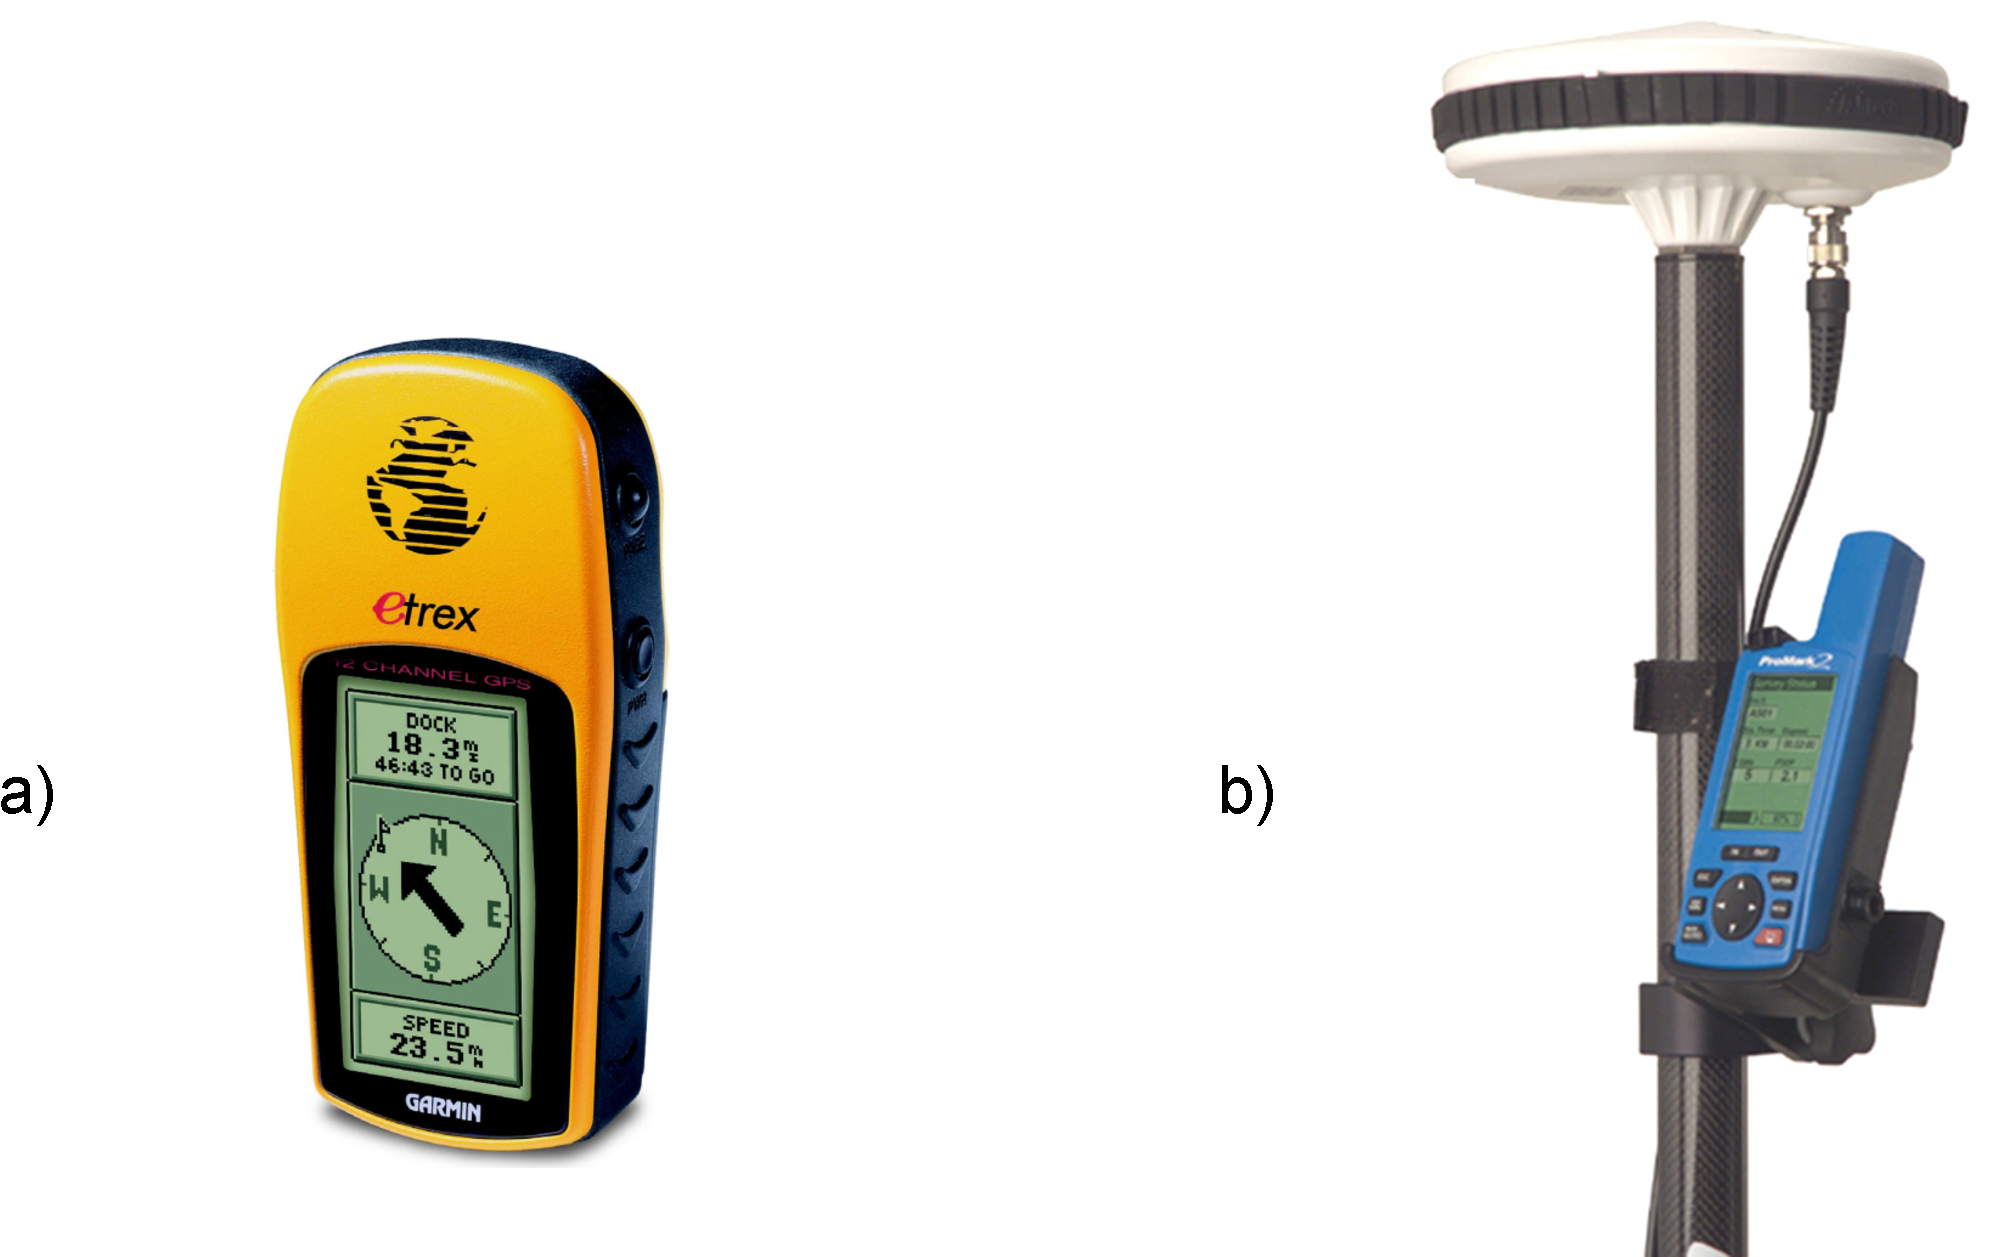
\includegraphics[width=.6\mycolumnwidth]{Fuentes_datos/gps.pdf}
\caption{\small Receptor GPS de bajo coste para uso general (a) y receptor GPS de alta precisi�n con antena externa (b)}
\label{Fig:gps_1} 
\end{figure}

\subsection{Operaciones con la unidad GPS}

La forma en que utilizamos el receptor GPS para recoger los datos que emplearemos posteriormente en el SIG puede ser muy variada en funci�n del tipo de dato, la precisi�n necesaria o las caracter�sticas del propio receptor. 

Los receptores de menor coste est�n generalmente pensados para ser de utilidad directamente en el campo, por ejemplo para localizar un punto concreto y conocer la direcci�n en la que hay que moverse para llegar hasta �l, pero tienen tambi�n capacidad para recoger coordenadas. Estas capacidades son las que resultan de inter�s desde el punto de vista de un SIG, ya que las coordenadas recogidas ser�n despu�s los datos que llevemos a este.

Por su parte, las unidades de mayor precisi�n est�n concebidas para tareas tales como levantamientos topogr�ficos, donde la toma de datos es lo fundamental, pero tambi�n para otras tales como replanteos, donde se requiere situar un punto de coordenadas conocidas. Al igual que en el anterior, las actividades que pueden llevarse a cabo con estos GPS y que interesan desde el punto de vista del SIG son aquellas que van a recoger coordenadas, pues son las que generan datos y convierten al GPS en una fuente de ellos.

Las capacidades de recogida de datos en una unidad GPS de bajo coste permiten almacenar puntos o trazados completos, encontr�ndose el operario inm�vil o bien en movimiento a lo largo de dicho trazado. Es habitual utilizar los vocablos ingleses de la terminolog�a GPS para denotar los distintos elementos que pueden recogerse, conoci�ndose a un punto de inter�s aislado como \emph{waypoint} y un trazado como \emph{track}. Una serie ordenada de \emph{waypoints} se conoce como \emph{route} (ruta).\index{Waypoint}\index{Track}\index{Route}

En el trabajo con el receptor GPS, el operario se puede detener en un punto cualquiera y memorizar las coordenadas del mismo, a�adiendo as� un \emph{waypoint} a la lista de los ya almacenados. Para crear un trazado, se suele disponer de funcionalidades de recogida autom�tica de puntos, de tal modo que el receptor memoriza estos a intervalos fijos de tiempo. El operario simplemente ha de desplazarse por el trazado y dejar que el receptor haga su trabajo mientras tanto. Dependiendo del tipo de dato que quiera obtenerse, la edici�n posterior en gabinete habr� de ser m�s o menos intensa. 

Esta edici�n no est� relacionada solo con la introducci�n de correcciones, sino con la interpretaci�n de los distintos puntos recogidos. Por ejemplo, para registrar el trazado de una calle, el operario puede recorrerla, pero es probable que no lo haga de forma perfectamente rectil�nea. El trabajo posterior con el conjunto de puntos debe resultar en la obtenci�n de una l�nea recta a partir de estos, y ello requiere la interpretaci�n de los datos disponibles.

Pese a que la precisi�n de estas unidades es limitada y no permiten t�cnicas avanzadas de correcci�n (tal precisi�n no es necesarias para las actividades tales como senderismo o navegaci�n para las que han sido dise�ados estos receptores), los GPS de uso cotidiano pueden ser una fuente de datos de primer orden para la recogida de datos. Un ejemplo significativo de ello es el proyecto OpenStreetMap\cite{webOSM}, un proyecto colaborativo para crear mapas libres  cuya principal fuente de datos son unidades GPS sencillas.\index{OpenStreetMap} Este proyecto es uno de los muchos que existen actualmente de este tipo, los cuales se engloban dentro de la idea de \emph{Informaci�n Geogr�fica Voluntaria o Participativa}, sobre la que hablaremos algo m�s adelante en el apartado \ref{VGI}.

Para trabajos de mayor precisi�n tales como levantamientos topogr�ficos, estos receptores no son, sin embargo, suficientes. El uso de receptores m�s precisos y de t�cnicas avanzadas es necesario para obtener precisiones mayores, que pueden ser incluso milim�tricas. 

Estos receptores pueden emplearse individualmente del mismo modo que se hace con un GPS de bajo coste, y registrar puntos de forma similar. La verdadera potencia, no obstante, se obtiene cuando se realizan mediciones con la ayuda de una o varias unidades adicionales, las cuales aportan valores de referencia que permiten aumentar la precisi�n. 

Entre el receptor m�vil y el de referencia se establece una \emph{l�nea base}, y en el c�lculo de la posici�n lo que se calcula es el vector $(x, y, z)$ que une a ambas. Se trata pues, de una medici�n relativa, ya que expresa la posici�n del receptor m�vil a partir de la del receptor de referencia. Puesto que la posici�n de este �ltimo se conoce con gran precisi�n y ese vector tambi�n se calcula con precisi�n, la posici�n buscada que se obtiene es altamente precisa.

La principal ventaja con respecto a m�todos topogr�ficos cl�sicos es que no es necesario que haya visibilidad entre los dos receptores. De esta forma, puede utilizarse una estaci�n de referencia aunque no sea visible desde un punto cuyas coordenadas queremos medir, y las l�neas base pueden ser de mayor longitud.

Otras ventajas tambi�n destacables son el hecho de que puede obtenerse una productividad mucho mayor, ya que una �nica unidad de referencia puede ser utilizada por varias unidades m�viles.

El n�mero de t�cnicas existentes en la actualidad para realizar este tipo de mediciones (ya sea con uno o con varios receptores) es variada. El hecho de que se busquen mediciones precisas hace que se realicen mediciones utilizando la fase de la portadora, que como vimos implica una mayor necesidad de tiempo para registrar correctamente una posici�n. En funci�n de las caracter�sticas de la linea base y los requerimientos concretos del trabajo, ser�n unas u otras las m�s adecuadas para cada caso. 

La diferencia principal entre estas t�cnicas es el tiempo necesario para la recogida de un punto. En general, un mayor tiempo equivale a una mayor precisi�n. Entre las t�cnicas habituales, cabe citar las siguientes:

\begin{itemize}
	\item \textbf{Est�tico}. En base a dos puntos de referencia (con una unidad GPS fija en cada uno de ellos), se calcula la posici�n de un tercero en un punto dado. Se trata del m�todo m�s preciso, pero requiere tiempos de observaci�n muy largos (superiores a una hora), lo que lo hace inadecuado para levantamientos o replanteos. Este tipo de procedimientos se emplean casi exclusivamente en trabajos geod�sicos y las lineas base pueden ser de gran longitud. 
	\item \textbf{Est�tico r�pido}. Igual que el anterior, pero con tiempos menores, del orden de 5--10 minutos por punto medido.	
	\item \textbf{Cinem�tico}. En el m�todo cinem�tico los tiempos son a�n menores que en el est�tico r�pido, del orden del minuto. El fundamento de la t�cnica es distinto a los anteriores, ya que tras la inicializaci�n el receptor m�vil puede desplazarse con m�s velocidad y no es necesario que se detenga durante un periodo largo de tiempo en cada punto, pero ello exige que durante el desplazamiento tanto la unidad m�vil como la fija de referencia mantengan la recepci�n de las se�ales, que han de ser de al menos cuatro sat�lites (preferiblemente cinco), y los mismos para ambas unidades. Si alguna de ellas pierde la conexi�n, se hace necesario repetir de nuevo el proceso de inicializaci�n \cite{Remondi1988IN}.
	
	Existe una gran variedad de procedimientos de tipo cinem�tico, cuya filosof�a es esencialmente la misma, pero bajo nombres distintos. Aunque pueden existir diferencias en los fundamentos te�ricos, la forma de proceder es en muchos casos muy similar. T�cnicas como \emph{Stop \& Go}\index{Stop \& Go} o \emph{pseudocinem�tico} pueden incluirse en este tipo de m�todos. En general, estos y otros se engloban bajo la denominaci�n de procedimientos cinem�ticos, aunque sus caracter�sticas sean distintas en cada caso. 
	
	Muchos de estos procedimientos vienen definidos por el equipo a utilizar, y los tiempos de paradas en cada punto medido, as� como otros aspectos, son recomendados por el propio fabricante. La forma m�s correcta de llevar a cabo una toma de datos en campo, en este caso, es seguir las indicaciones concretas del fabricante de para cada producto.
	
	Un caso particular dentro de los m�todos cinem�ticos es el \emph{cinem�tico en tiempo real} (RTK)\footnote{Real Time Kinematic}, en el que, a diferencia de los anteriores, las correcciones necesarias se efect�an en tiempo real y no requieren postproceso. Se trata de la t�cnica m�s actual, y proporciona al operario mediciones exactas de su posici�n de forma instant�nea, con las ventajas que ello conlleva. Las mediciones son m�s precisas, ya que el operario que las toma conoce el valor recogido en el mismo momento de hacer la medici�n, y puede de esa forma realizar una comprobaci�n en el acto. Informaci�n m�s detallada sobre esta t�cnica puede encontrarse en \cite{Rizos1998BCG}.
\end{itemize}\index{Real Time Kinematic}

Para profundizar m�s al respecto, en \cite{Asenjo1997UPV} puede encontrarse informaci�n sobre la realizaci�n de levantamientos con GPS, as� como en \cite{GPSUSArmy}.

En base a los ejemplos anteriores, y para concluir esta parte, podemos dar una clasificaci�n de las operaciones con un receptor GPS en funci�n de tres criterios b�sicos: el n�mero de unidades que se emplean simult�neamente, el movimiento (o ausencia de �l) del receptor y el momento en el que se obtiene el dato ya listo para su utilizaci�n posterior.

Seg�n el n�mero de unidades, tenemos:

\begin{itemize}
	\item \textbf{Absolutas}. Se tiene un �nico receptor y un �nico operario. La posici�n se calcula con la informaci�n de los sat�lites, sin apoyo de otra unidad adicional.
	\item \textbf{Relativas}. Se emplea una unidad adicional a modo de referencia. Las medidas se basan en la informaci�n de los sat�lites y la que aporta dicha unidad de referencia, y la posici�n se calcula en relaci�n a esta en lugar de en t�rminos absolutos. Estas operaciones alcanzan un grado de precisi�n mayor que las de tipo absoluto.
\end{itemize}

Atendiendo al movimiento del receptor encontramos:

\begin{itemize}
	\item \textbf{Est�ticas}.
	\item \textbf{Cinem�ticas}.
	\item \textbf{Variantes intermedias}.
\end{itemize}

Por �ltimo, en funci�n de la obtenci�n de datos, distinguimos:

\begin{itemize}
	\item \textbf{En tiempo real}. Las correcciones pertinentes se realizan en el acto, y el resultado que se visualiza en el receptor o se almacena en este ya ha sido filtrado y corregido.
	\item \textbf{Con necesidad de postproceso}. Las correcciones se realizan en gabinete posteriormente, con informaci�n que el receptor no posee o no es capaz de procesar de modo inmediato durante su utilizaci�n.
\end{itemize}

\subsection{Integraci�n de GPS y SIG}

\index{GPS!integraci�n con SIG}

La utilidad de un GPS como fuente de datos para el trabajo en un SIG es innegable. Multitud de trabajos que requieren la toma de datos en campo y la medici�n de coordenadas pueden efectuarse ventajosamente con equipos GPS, y la informaci�n derivada de ese uso puede ser posteriormente incorporada a un SIG.

EL GPS puede emplearse como una fuente de datos est�tica (se utiliza como herramienta para la creaci�n de una capa de informaci�n geogr�fica y esta despu�s se emplea en el SIG de la forma habitual), o bien para la obtenci�n de datos en tiempo real. Los SIG sobre dispositivos m�viles (v�ase el apartado \ref{SIG_Moviles}) pueden aprovechar los receptores GPS que estos dispositivos habitualmente incorporan, y alimentarse con los datos de dichos receptores en tiempo real.

Un caso particular de esto son los cada d�a m�s populares navegadores GPS. Estos dispositivos aunan el receptor GPS y una aplicaci�n de tipo SIG que presenta un visor y permite ejecutar un n�mero reducido de procesos, en concreto los de c�lculo de rutas �ptimas entre dos puntos a trav�s de una red de comunicaci�n (apartado \ref{Rutas_optimas}). Uno de los puntos (el de destino) es fijado por el usuario, mientras que el punto de origen es el punto actual en que se encuentra el dispositivo, que se obtiene a partir del GPS.

Como herramientas est�ticas, el trabajo en campo con un GPS genera un conjunto de puntos o de trazados, que pueden f�cilmente transferirse al ordenador para poder trabajar con ellos. Este trabajo puede realizarse dentro de un SIG, ya que, o bien este incluye la capacidad de importar los archivos generados por el GPS, o el software que acompa�a a dicho GPS incorpora herramientas para ayudar en la comunicaci�n entre SIG y GPS.

Adem�s de la informaci�n posicional que deriva del sistema GPS, los receptores GPS pueden incorporar elementos que permitan la entrada de la componente tem�tica asociada a las distintas entidades, es decir, los atributos. Si solo se registra la componente espacial, la informaci�n que se almacena en el GPS es de mucha menos utilidad que si se acompa�a de atributos.

Las funcionalidades incorporadas en el receptor suelen ser sencillas, pero permiten que desde este se pueda llevar a cabo todo el proceso de creaci�n de la capa que posteriormente se emplear� en el SIG. El trabajo de campo incluye de este modo tanto el registro y creaci�n de las entidades como la edici�n de las propiedades no espaciales de estos. Existe, no obstante, la posibilidad de completar la fase de introducci�n de atributos en el SIG, durante el trabajo en gabinete, lo cual en ocasiones resulta m�s sencillo y pr�ctico.

El volumen de trabajo que se requiere una vez que los datos han sido recogidos depender� tambi�n de las necesidades de precisi�n que se presenten y del tipo de trabajo en que se enmarque dicha recogida de datos. La realizaci�n de correcciones y la edici�n avanzada de los datos no puede en ocasiones realizarse dentro de un SIG, ya que este no dispone de las herramientas necesarias para un tratamiento avanzado de los datos del GPS. El SIG est� preparado para trabajar con las coordenadas que salen del GPS, pero este puede almacenar m�s datos (datos <<en bruto>>), que pueden procesarse en gabinete para la obtenci�n de dichas coordenadas de forma m�s precisa. Para realizar esta tarea  es necesario software especializado, y las funcionalidades del SIG se emplear�n posteriormente, cuando ya se hayan verificado los datos del GPS y elaborado las capas correspondientes.

Para el lector interesado, una referencia completa sobre el uso de GPS de cara a la integraci�n de los datos en un SIG es \cite{Steede2000ESRI}.  En el ya mencionado apartado \ref{SIG_Moviles} veremos con detalle la tecnolog�a de los SIG m�viles, un �mbito en el que SIG y GPS se unen para conformar herramientas conjuntas. 

\section{Informaci�n Geogr�fica Voluntaria}
\label{VGI}

Hemos mencionado ya que los dispositivos tales como receptores GPS de bajo coste pueden emplearse para recoger informaci�n geogr�fica y crear datos geogr�ficos, y que cuando esto se une a los conceptos participativos de la denominada Web 2.0, surgen iniciativas de gran inter�s en las que el usuario de a pie, sin necesidad de una formaci�n espec�fica como cart�grafo, puede aportar sus datos para que otros los exploten posteriormente. Aunque no se trata de una fuente de datos como tal, y los elementos y dispositivos empleados ya los hemos visto a lo largo de este cap�tulo, el cambio que supone la inclusi�n de una filosof�a acorde con las ideas de la Web 2.0 es tan notable que merece ser tratado por separado. No se trata de un cambio en la propia toma o preparaci�n de datos, o de una tecnolog�a nueva que se aplique a estos, sino de un cambio social y filos�fico que redefine el propio concepto de la informaci�n geogr�fica en lo que a la creaci�n del dato geogr�fico respecta, y cuyas consecuencias son ciertamente importantes, ya que abren el �mbito de la creaci�n cartogr�fica a un nuevo y amplio grupo de personas.\index{Web 2.0}

Se conoce como \emph{Informaci�n Geogr�fica Voluntaria o Participativa} (en ingl�s Volunteered Geographical Information, VGI)\cite{Goodchild2007VGI} al uso de Internet para crear, gestionar y difundir informaci�n geogr�fica aportada voluntariamente por usuarios de la propia red. El conjunto de herramientas y t�cnicas que emplean esos usuarios para aportar su informaci�n conforma lo que se ha dado en llamar \emph{neogeograf�a}. La comparaci�n entre proyectos de creaci�n de VGI y la bien conocida Wikipedia, tal y como se coment� en otro punto anterior en este mismo cap�tulo, sirve perfectamente para ilustrar qu� es lo que entendemos por VGI y neogeograf�a.
\index{Neogeograf�a}\index{VGI}\index{Informaci�n Geogr�fica Voluntaria|see{VGI}}\index{Wikipedia}

En el caso particular de esta �ltima, la neogeograf�a ha supuesto un profundo cambio en algunas de las ideas b�sicas de la cartograf�a, modificando asimismo la concepci�n tradicional de la informaci�n geogr�fica, sus caracter�sticas o el papel que esta ven�a desempe�ando en muchos �mbitos (o incluso d�ndole un papel en campos donde con anterioridad el uso de informaci�n geogr�fica era escaso). Algunas de las ideas principales sobre la neogeograf�a son las siguientes:

\begin{itemize}
	\item Popularizaci�n y democratizaci�n. La producci�n cartogr�fica ha estado siempre en manos de gobiernos u organismos, y en muchas ocasiones fuertemente censurada debido a su elevado valor estrat�gico. Con la VGI, la creaci�n de informaci�n geogr�fica se democratiza y se convierte en un proceso participativo libre y sin restricciones.  Se invierte el esquema <<hacia abajo>> de producci�n y uso de informaci�n geogr�fica.
	\item Los ciudadanos se convierten en <<sensores>> y tienen mayor consciencia de su realidad geo--espacial.
	\item Se elimina parte del <<misticismo>> de la producci�n de informaci�n geogr�fica	
\end{itemize}

En parte, estas ideas son tambi�n comunes a otros fen�menos basados en la Web 2.0, ya que todas se fundamentan en una mayor democratizaci�n de la informaci�n, sea esta geogr�fica o no. Tambi�n se comparten algunos de los problemas o cr�ticas que otros �mbitos han recibido al adoptar esquemas de producci�n similares. Por ejemplo, la calidad de la informaci�n es puesta en entredicho al promover la participaci�n de todo tipo de personas, con independencia de su perfil. En el caso de la informaci�n geogr�fica, con una producci�n tradicionalmente como hemos dicho limitada a profesionales muy especializados, esto es especialmente relevante. Con la proliferaci�n de la VGI, se da voz y poder sobre la informaci�n geogr�fica a individuos en gran medida sin formaci�n, que no obtienen un beneficio tangible obvio y no pueden aportar garant�as de veracidad o autoridad alguna. Esto puede plantear dudas l�gicas acerca de la conveniencia de usar esa informaci�n.

No debe olvidarse no obstante, que la Web 2.0 tambi�n tiene sus mecanismos de regulaci�n, y que en otros casos ya se ha demostrado que, para otros tipos de informaci�n, la calidad y rigor de esta no es inferior a la creada con esquemas m�s cl�sicos y menos abiertos. Un hecho particularmente curioso que tiene lugar a este respecto con la informaci�n geogr�fica es el relacionado con los denominados \emph{elementos trampa}, y particularmente con el m�s popular de ellos, las \emph{calles trampa}. Aunque se trata de una pr�ctica negada por buena parte de los productores de cartograf�a, es sabido que estos introducen elementos err�neos (tales como una calle inexistente en un callejero) como medida para proteger sus derechos de autor y poder reconocer copias ilegales. En el caso de la VGI, puesto que no existe esa necesidad ya que la informaci�n generada y aportada por los voluntarios es libre, no existen este tipo de errores intencionados. La comparaci�n de informaci�n geogr�fica cl�sica con VGI ha puesto de manifiesto que se trata de una pr�ctica real que, obviamente, disminuye la calidad del dato geogr�fico.

Por otra parte, el hecho de que se use equipo de bajo coste y los usuarios no sean t�cnicos especializados no es necesariamente un problema. Un usuario sin formaci�n no est� capacitado para efectuar un levantamiento topogr�fico preciso, pero s� para situarse delante de la puerta de una tienda y marcar su posici�n, a�adiendo esta a un proyecto que catalogue los comercios de la zona y su localizaci�n. Este tipo de informaci�n geogr�fica, de puntos de inter�s muchas veces no recogidos en cartograf�a m�s especializada, constituye una gran parte de la VGI, y las metodolog�as e instrumental con que se crea son m�s que suficientes para otorgarle validez y precisi�n adecuada al uso del que posteriormente va a ser objeto.

En resumen, la neogeograf�a es en la actualidad un fen�meno que no debe dejarse de lado, ya que los proyectos que aglutina se est�n convirtiendo paulatinamente en proveedores fundamentales de datos cuya calidad en muchos casos es excelente.

Aunque las hemos tratado dentro de este cap�tulo dedicado a las fuentes de datos, la VGI y la neogeograf�a tienen una indudable vinculaci�n con todo lo desarrollado en la parte de este libro dedicada al factor organizativo, ya que se trata de un fen�meno social m�s que t�cnico. De igual modo, el cap�tulo \ref{SIG_movil}, dedicado a los SIG m�viles, est� tambi�n muy relacionado con ambas, puesto que son los dispositivos y aplicaciones que veremos entonces, as� como los servicios sobre ellos, los que han posibilitado el desarrollo de la neogeograf�a y la abundante producci�n actual de VGI. \index{SIG m�vil}


\section{Sobre cartograf�a de elevaciones}

La cartograf�a de elevaciones es probablemente la de mayor importancia de entre todas las que se emplean de forma habitual dentro de cualquier proyecto SIG. Su relevancia deriva del hecho fundamental de que la practica totalidad de procesos que se estudian en un SIG tienen alg�n tipo de componente relacionada con el terreno y su relieve, y por tanto puede obtenerse amplia informaci�n sobre dichos procesos a partir de una capa con datos de elevaci�n.

Como dato relevante, dedicaremos en este libro un cap�tulo entero, el \ref{Geomorfometria}, al conjunto de operaciones de an�lisis basadas en el MDE\index{Modelo Digital de Elevaciones}, que van desde el simple c�lculo de pendientes hasta la extracci�n de par�metros m�s complejos, pasando por la definici�n del comportamiento hidrol�gico de una zona seg�n las caracter�sticas de su relieve, entre otros. Asimismo, gran n�mero de otras formulaciones que veremos en la parte dedicada a procesos tienen su principal aplicaci�n sobre datos de elevaci�n, en particular los m�todos de interpolaci�n que veremos en el cap�tulo \ref{Creacion_capas_raster}, y que nos permitir�n crear cartograf�a de elevaciones en formato r�ster. Este es, como veremos, el formato preferido para el an�lisis de la cartograf�a de elevaciones, ya que ofrece un mayor abanico de posibilidades frente a otros.\index{Interpolaci�n}

Aunque el formato r�ster es el m�s indicado para llevar a cabo los an�lisis correspondientes, la cartograf�a de elevaciones puede crearse originalmente con muy diversas caracter�sticas. De igual modo, y debido tambi�n a la gran importancia de este tipo de capas, su origen puede ser muy variado, ya que son muchas las t�cnicas distintas que existen para su creaci�n. Es de inter�s, por tanto, exponer en este cap�tulo sobre fuentes de datos algunas de las ideas principales relativas a la creaci�n de capas de elevaciones, las caracter�sticas de estas o las ideas fundamentales que residen tras las metodolog�as m�s importantes. Posteriormente, esto nos ayudar� a entender mejor las restantes formulaciones y conceptos relativos al manejo y an�lisis de este tipo de cartograf�a, abundantes en este libro como ya se ha dicho.

A modo de resumen, he aqu� una lista de metodolog�as a partir de las cuales puede obtenerse cartograf�a de elevaciones, gran parte de las cuales han sido tratadas con detalle antes en este mismo cap�tulo.

\begin{itemize}
\item \textbf{GPS}. Como ya sabemos, un GPS toma datos no solo de la posici�n que ocupa en coordenadas $x$ e $y$, sino tambi�n su elevaci�n. La utilizaci�n de GPS permite obtener una nube de puntos de elevaci�n, aunque si esta ha de cubrir un territorio amplio y con cierta precisi�n en las medidas, resulta poco id�neo el trabajar con esta tecnolog�a, ya que es costoso en tiempo. Es m�s adecuada para obtener levantamientos precisos de �reas m�s reducidas, donde se demuestra como una herramienta sumamente eficaz.
\item \textbf{Digitalizaci�n de curvas de nivel}. En ocasiones la cartograf�a de elevaciones ya existe, aunque no en el formato adecuado para su empleo en un SIG. Ya conocemos los m�todos de digitalizaci�n de entidades, tanto manuales como autom�ticos, y ya sea en pantalla o en equipo especializado, y mediante ellos podemos digitalizar las curvas de nivel, obteniendo una capa de l�neas con la informaci�n altitudinal que contiene un mapa topogr�fico habitual.\index{Digitalizaci�n!de curvas de nivel}\index{Curva!de nivel!digitalizaci�n}
\item \textbf{Estereograf�a}. A partir de pares estereosc�picos, y con el concurso de una estaci�n fotogram�trica digital pueden delinearse l�neas o puntos de una elevaci�n dada, digitalizando as� la informaci�n altim�trica. El procedimiento es similar a la simple digitalizaci�n de curvas de nivel, solo que en este caso estas no est�n presentes expl�citamente en las im�genes de partida, y se infieren a partir de la visualizaci�n tridimensional de las mismas.\index{Estereograf�a}
\item \textbf{Interferometr�a}. La interferometr�a es una t�cnica cuyos fundamentos son en cierta medida similares a los de la estereograf�a, pues se basan en la informaci�n recogida de un punto concreto desde dos puntos distintos. Si en el caso de emplear simples im�genes esto permit�a crear una imagen tridimensional, en el caso de la interferometr�a el estudio de las diferencias de fases entre las ondas recibidas en dos puntos distintos permite el c�lculo de distancias. Se trata, por tanto, de un proceso automatizado, que requiere menos intervenci�n que en el caso de la restituci�n fotogram�trica.\index{Interferometr�a}

Un uso muy habitual de esta t�cnica es con los denominados \emph{Radares de Apertura Sint�tica}\footnote{Synthetic Aperture Radar (SAR)}, utilizado por ejemplo en el caso de la misi�n SRTM, que rese�amos anteriormente como producto importante. La medici�n desde dos puntos puede hacerse con dos pasadas de sat�lite (caso por ejemplo del ERS) o bien en una sola si la plataforma dispone de dos receptores separados una cierta distancia (caso del SRTM). En \cite{SARInterferometry} puede encontrarse una descripci�n detallada de este tipo de t�cnicas y las etapas que comprenden.
\item \textbf{LiDAR}. La t�cnica m�s avanzada en la actualidad es el uso de aparatos de altimetr�a basados en l�ser, como el LiDAR, que ya hemos visto en este mismo cap�tulo. El LiDAR ofrece posibilidades muy interesantes tales como la obtenci�n de MDE y MDS (Modelo Digital de Superficie) por separado. \index{Radar de Apertura Sint�tica}\index{Synthetic Aperture Radar}\index{LiDAR}\index{SRTM}\index{Modelo Digital de Superficie}

El resultado de un trabajo con LiDAR es una nube de puntos, normalmente en un n�mero muy elevado debido a la precisi�n del instrumento, la cual puede emplearse para crear otro tipo de capas, tales como capas r�ster. El nivel de postproceso que se requiere para la obtenci�n final de una capa es mucho menor que con otras t�cnicas.
\end{itemize}

A la hora de plantear un proyecto SIG, debe elegirse entre estas fuentes, tanto si se desea adquirir la cartograf�a ya elaborada como si se desea crearla a partir de otras fuentes. La variedad de opciones existentes es grande, y cada una de ellas tiene sus caracter�sticas peculiares. Para saber m�s al respecto, algunas referencias donde puede encontrarse una comparaci�n entre las metodolog�as anteriores son \cite{Nikolakopoulos2006IJRS}, \cite{Mercer1999ISPRS} y \cite{Mercer2001PW}.

\section{Formatos de archivo}
\label{Formatos_archivo}

Como hemos visto, las fuentes de datos son muy variadas, y a la hora de elaborar un proyecto SIG podemos recoger datos de muchas procedencias distintas. Conocer todas estas fuentes de datos es importante para elaborar una base de datos geogr�fica que permita obtener los mejores resultados posibles, pero tambi�n lo es el conocer la forma en que esos datos pueden obtenerse. Los datos geogr�ficos se van a almacenar en archivos, existiendo muchos formatos de archivo distintos para recoger un mismo conjunto de datos.

Estos archivos son la materializaci�n de los modelos de almacenamiento que ve�amos en el apartado \ref{Modelos_almacenamiento}, y su existencia obedece a distintas razones. Pueden haber sido definidos por alguna casa comercial para ser utilizados en su software, por un colectivo, o bien pueden ser est�ndares internacionales definidos para tratar de homogeneizar la forma en que se presentan los datos dentro de un determinado �mbito de trabajo.

Datos de una misma procedencia pueden presentarse de forma distinta si se emplean diferentes formatos de archivo. Las circunstancias por las cuales se opta por uno u otro formato pueden basarse �nicamente en el hecho de que el software empleado soporte o no dicho formato, pero deber�an fundamentarse en las propias caracter�sticas del formato y lo adecuadas que estas son para recoger la informaci�n con la que trabajamos.

La existencia de muchos formatos de archivo dificulta el trabajo con los datos en un SIG, principalmente porque ning�n SIG implementa la capacidad de poder <<leer>> todos los formatos existentes. La interoperabilidad y la comunicaci�n entre distintos SIG, o incluso entre un SIG y otras aplicaciones (bases de datos, aplicaciones para manejo de im�genes, aplicaciones CAD) no es completa, y el aprovechamiento de todos los datos disponibles dentro de un proyecto requiere normalmente tiempo para la gesti�n adecuada de datos en formatos variados.\index{CAD}

Un problema m�s serio, no obstante, es el desconocimiento por parte de los usuarios de las implicaciones que tiene el uso de uno u otro formato, ya que en ocasiones no permiten aprovechar de modo pleno los datos de que se dispone. Por ejemplo, dentro de un SIG es habitual emplear datos procedentes de CAD. Los datos en un CAD se almacenan en formatos de datos definidos por esas aplicaciones CAD, los cuales han sido definidos para satisfacer las necesidades del �mbito de trabajo en el que se han desarrollado (el dise�o asistido por ordenador). Aunque los SIG pueden leer esos formatos de archivo y se encuentra informaci�n muy valiosa almacenada en ellos, no son ideales para el manejo de capas de datos SIG (en este caso, capas vectoriales), y es importante conocer este hecho.

La existencia de librer�as que act�an a modo de interpretes facilita el desarrollo de aplicaciones SIG con capacidades de lectura y escritura en muchos formatos distintos, pero a�n as� se requiere un cierto grado de comprensi�n de estos por parte del usuario.

Debemos pensar asimismo que los formatos de archivo no solo se emplean en un proyecto SIG para los datos de entrada, sino tambi�n para almacenar los resultados que se generan a lo largo de ese proyecto. Estos datos ser�n utilizados en el propio SIG en otras ocasiones posteriores, o bien en otros programas. De este modo, tomamos datos que pueden provenir de aplicaciones y fuentes diversas, pero tambi�n <<damos>> datos a esas aplicaciones, por lo que la comunicaci�n es bidireccional. Puesto que es a trav�s de archivos como dicha comunicaci�n se produce, y estos tienen que tener un formato dado, el conocimiento de estos formatos mejora tanto esa comunicaci�n como la potencialidad de nuestros datos para todo tipo de uso, ya sea dentro o fuera de un SIG.

En esta secci�n no se pretende describir todos los formatos existentes, ya que estos son demasiados y ello no tendr�a sentido. Se describir�n solo los m�s populares (que no siempre han de ser necesariamente los mejores) para que el lector obtenga un conocimiento general de \emph{c�mo} se van a presentar sus datos, y a trav�s de estos formatos se describir�n los principales enfoques existentes, que son los que realmente ha de conocer un usuario de SIG para saber discernir si un formato es o no adecuado para sus datos y las operaciones que quiere aplicar sobre ellos.

Junto con estos formatos de archivo, en el cap�tulo \ref{Estandares} se presentan los est�ndares de datos, que tambi�n se emplean para el intercambio y almacenamiento de datos SIG, y que presentan una relaci�n estrecha con el contenido de esta secci�n. El capitulo \ref{Bases_datos}, que veremos dentro de esta misma parte, tambi�n guarda relaci�n con este apartado, pues estudia las diferentes formas en que los SIG han solucionado a lo largo del tiempo el acceso a los datos, incluyendo entre ellas el acceso directo a archivos.

\subsection{Formatos para datos r�ster}

Los formatos de archivo para datos r�ster son muy abundantes, existiendo numerosas alternativas con diferencias en ocasiones notables entre s�. Debido a que uno de los datos r�ster m�s habituales en un SIG son las im�genes, a los formatos de datos espec�ficos para datos r�ster hay que sumar aquellos ya existentes para el almacenamiento de im�genes, que son de por s� muy variados. Estos formatos, adaptados a la naturaleza particular de las im�genes de un SIG, pueden emplearse para almacenar datos r�ster y son de hecho de uso habitual en el �mbito de los Sistemas de Informaci�n Geogr�fica.

\subsubsection{Formatos para im�genes}

Como ya sabemos, las im�genes son un tipo de dato muy habitual en un SIG, y estas se corresponden con el modelo de datos r�ster. Por ello, los formatos de archivo empleados para el almacenamiento de im�genes digitales se emplean tambi�n para las im�genes particulares que utilizamos en un SIG (por ejemplo, fotograf�as a�reas o mapas escaneados, seg�n vimos antes en este mismo cap�tulo), e incluso para otros datos r�ster que no son im�genes como tales, como por ejemplo un Modelo Digital de Elevaciones.

Los formatos de archivo para im�genes son adecuados para recoger los colores de las im�genes, pero esto no es suficiente a la hora de almacenar otros valores (por ejemplo, valores decimales) o bien cuando son necesarios un n�mero m�s elevado de bandas, como en el caso de im�genes hiperespectrales. 

Una imagen en blanco y negro o en escala de grises contiene una banda. Una imagen en color contiene tres, ya que los colores se expresan como una terna de colores b�sicos: rojo, verde y azul. Este es el fundamento del modelo de color RGB, en el cual todo color es la combinaci�n de distintas intensidades de los anteriores colores b�sicos. Las intensidades de cada banda (o las intensidades de la �nica banda en el caso de una imagen en escala de grises) se expresan habitualmente con valores entre 0 y 255, un rango que resulta insuficiente para el manejo de otras variables tales como las variables f�sicas que pueden emplearse en un SIG, ya que estas presentan valores continuos.  \index{Modelo!de color RGB}

En estos casos, los formatos de im�genes no son adecuados en su forma original, y deben o bien adaptarse o bien emplearse formatos m�s espec�ficos que tengan en cuenta el tipo particular de im�genes que se almacenan.

Otro problema es la presencia de celdas sin datos. La existencia de celdas sin datos es un hecho que no contemplan los formatos de im�genes. A estas celdas se les asigna un valor establecido por defecto, el cual ha de definirse en el propio archivo para que despu�s sea reconocido por el SIG (para que sepa que, donde aparezca ese valor, realmente no existen datos), pero muchos formatos de imagen no puede almacenarlo. Una posible soluci�n es la utilizaci�n de formatos que permitan transparencia. En estos, se puede especificar un color como transparente, que a efectos de su utilizaci�n en un SIG puede considerarse como indicaci�n de la ausencia de datos. Estos formatos, no obstante, no son los m�s adecuados para datos SIG, y esta soluci�n no resuelve por completo esta deficiencia.

Otra deficiencia de los formatos de im�genes es que no pueden recoger la referencia geogr�fica de la imagen. Salvo que las im�genes sean utilizadas en un SIG, no hay necesidad de que estas contengan informaci�n tal como el tama�o de p�xel (los metros que cada p�xel representa en la realidad) o las coordenadas de la zona que recogen. Por ello, las definiciones de los formatos de imagen, al estar pensadas para recoger meras im�genes digitales (y no im�genes de sat�lite o a�reas destinadas a un an�lisis espacial), no tienen en cuenta estas necesidades.

Una forma habitual de resolver esto es acompa�ar cada fichero de imagen con un peque�o fichero de texto plano donde se contengan los datos geogr�ficos correspondiente a la imagen. Este fichero se denomina \emph{World File}, y tiene una forma como la siguiente:\index{World file}

\begin{minipage}{\linewidth}
\begin{verbatim}
1.0
0.0
0.0
-1.0
691200.0
4576000.0
\end{verbatim}
\end{minipage}

El significado de las anteriores l�neas es el siguiente:
\begin{itemize}
\item L�nea 1. Tama�o de celda en la direcci�n Este--Oeste
\item L�neas 2 y 3. �ngulos de rotaci�n del plano respecto a los ejes X e Y. Estos valores son siempre iguales a cero.
\item L�nea 5. Tama�o de celda en la direcci�n Norte--Sur, con signo negativo
\item L�neas 6 y 7. Coordenadas \emph{x} e \emph{y} del p�xel superior izquierdo de la imagen.
\end{itemize}

Este \emph{World File} tiene el mismo nombre que el archivo de imagen, y su extensi�n se forma con la primera y la �ltima letra de la extensi�n de dicho archivo, y la letra \texttt{w}. As�, para un archivo \texttt{imagen.tif}, se tendr� un archivo \texttt{imagen.tfw}. Cuando el SIG abre la imagen, busca dicho fichero y, en caso de existir este, toma de �l la informaci�n que necesita para poder incorporar la imagen al SIG de forma completa, de tal modo que sobre ella puedan llevarse a cabo an�lisis espaciales u operaciones como la digitalizaci�n en pantalla (heads--up) que hemos visto anteriormente.
\index{Heads--up}

Por �ltimo, un aspecto importante de los archivos de imagen es el tipo de compresi�n que utilizan. Las im�genes con las que se trabaja en un SIG pueden ser muy voluminosas, y para almacenarlas es necesaria gran cantidad de espacio (puede ser del orden de \emph{gigabytes} para el caso de im�genes de alta resoluci�n). Por esta raz�n, los formatos de imagen, especialmente los que han sido creados  espec�ficamente para im�genes SIG, incluyen alg�n m�todo de compresi�n para disminuir el volumen del archivo.

En el apartado relativo a los modelos de almacenamiento vimos algunas ideas sobre compresi�n, presentando la codificaci�n \emph{run--length}. Esta es una estrategia para almacenar la informaci�n de forma que se minimice el tama�o de los datos necesarios, y en base a los datos recogidos puede recuperarse toda la imagen de forma exacta. Es decir, la utilizaci�n de estas formas de compresi�n no supone una degradaci�n de la informaci�n contenida en la imagen, y nada de esta se pierde en el proceso. Podemos comprimir y descomprimir la imagen tantas veces como queramos, y el resultado siempre ser� el mismo, fiel a la imagen original. Un formato de archivo que cumple esto se dice que emplea un m�todo de compresi�n \emph{sin p�rdidas}.\index{Compresi�n!sin p�rdidas}\index{Run--Length Encoding}	

Por el contrario, existen otros m�todos de compresi�n \emph{con p�rdidas}, en los cuales se pierde informaci�n y la imagen resultante, adem�s de ocupar menos espacio, tiene una menor calidad y no es exactamente igual a la original, sino simplemente muy similar a esta. Los algoritmos de compresi�n con p�rdidas toman de la imagen original la informaci�n m�s importante para despu�s recrear esta, ignorando la menos relevante, que se pierde en aras de obtener un menor volumen de almacenamiento.\index{Compresi�n!con p�rdidas}

Siempre que sea posible, los formatos de compresi�n sin p�rdidas deben preferirse frente a los que utilizan algoritmos de compresi�n son p�rdidas, ya que no se pierde informaci�n alguna con ellos. En funci�n de las necesidades que se tenga con respecto a las im�genes a almacenar, debe elegirse el formato adecuado, considerando siempre la degradaci�n que la compresi�n con p�rdidas implica.

Algunos formatos de imagen que emplean compresi�n con p�rdidas son altamente populares, ya que se emplean para tareas donde la reducci�n de tama�o de los ficheros es prioritaria, y este tipo de compresi�n ofrece una reducci�n en general mayor que la de los algoritmos sin p�rdidas. As�, por ejemplo, las im�genes que se incorporan en paginas Web han de ser de peque�o tama�o para agilizar su carga, y ese tama�o resulta un factor decisivo, especialmente donde la velocidad de conexi�n es limitada. Para el trabajo con un SIG, no obstante, la calidad de la imagen es de mucho mayor importancia que su tama�o, y los formatos de compresi�n sin p�rdidas responden mejor a las necesidades del almacenamiento de datos SIG.

En la imagen \ref{Fig:Compresion_con_perdidas} puede verse el efecto de la utilizaci�n de compresi�n con p�rdidas.

\begin{figure}
\centering
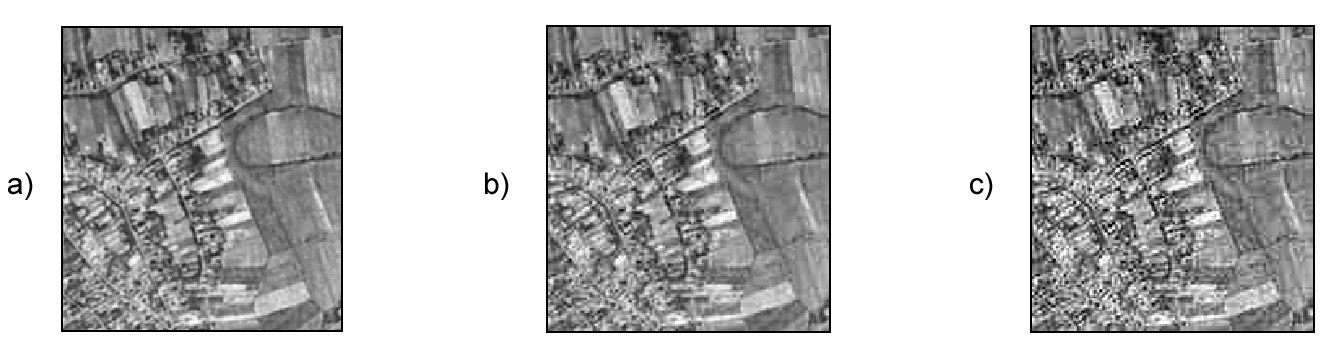
\includegraphics[width=.9\textwidth]{Fuentes_datos/Compresion_con_perdidas.png}
\caption{\small Efectos de la utilizaci�n de algoritmos de compresi�n con p�rdidas. a) Imagen original. b) Imagen almacenada mediante compresi�n con p�rdidas. c) Imagen tras diez procesos de lectura y almacenamiento en un formato de archivo con compresi�n con p�rdidas. El efecto de la degradaci�n sucesiva que la imagen sufre es claramente apreciable.}
\label{Fig:Compresion_con_perdidas} 
\end{figure}

\subsubsection{Formatos para datos SIG}

Junto con los formatos de archivo para im�genes, los SIG r�ster han desarrollado sus propios formatos para el almacenamiento de capas r�ster en general, y en particular de aquellas que no representan im�genes, tales como capas de variables f�sicas.

Estos formatos est�n pensados para las caracter�sticas de estas capas, que habitualmente recogen valores decimales (a diferencia de los valores enteros de los Niveles Digitales de una imagen), y que no suelen contener m�s que una �nica banda.

Adem�s de corresponder a un SIG particular (pr�cticamente cada SIG tiene su propio formato de archivo r�ster), otras aplicaciones que trabajan con este tipo de datos, tales como todas aquellas que usan por una u otra raz�n informaci�n de elevaciones, tambi�n disponen de sus formatos particulares. Muchos SIG pueden leer algunos de estos formatos junto con los suyos propios o los de otros SIG.

A la hora de almacenar una capa tal como un Modelo Digital del Terreno o cualquier otra de similar �ndole, estos formatos son preferibles en general a las im�genes, ya que los formatos de imagen, aunque ya hemos visto que pueden adaptarse y ser en algunos casos plenamente operativos para otro tipo de variables, no son formatos puramente pensados para este tipo de informaci�n.

\subsubsection{Principales formatos existentes}

Dentro de la gran variedad de formatos existentes, he aqu� una breve lista de los principales, los cuales suelen encontrarse con frecuencia a lo largo del desarrollo de un proyecto SIG habitual.

Dentro de los formatos para im�genes, cabe destacar los siguientes:

\begin{itemize}
	\item \textbf{Tagged Image File Format (tif)}. Se trata de un formato complejo y altamente flexible, con muchas variantes distintas. Puede incorporar tanto compresi�n con p�rdidas como sin p�rdidas, en funci�n del algoritmo que se utilice. Se utiliza habitualmente tanto en el �mbito del tratamiento de im�genes como en el �mbito SIG. En este �ltimo, permite tambi�n el almacenamiento de valores decimales, siendo apto para almacenar capas que no representen im�genes como tal.
	Es un formato habitualmente generado por los esc�neres, con lo cual es frecuente su utilizaci�n al trabajar con cartograf�a escaneada, seg�n vimos antes en este mismo cap�tulo.
	Existe una variante denominada GeoTIFF, que permite incorporar en el propio fichero la georreferencia de la imagen, haciendo innecesario el uso de un \emph{World File} asociado.
	\item \textbf{Joint Photographic Experts Group (jpg o jpeg)}. Un formato muy popular para im�genes (todas las c�maras digitales lo utilizan), no es sin embargo adecuado para el trabajo con SIG. Incorpora compresi�n con p�rdidas (el ejemplo de la figura \ref{Fig:Compresion_con_perdidas} ha sido realizado utilizando este formato), y no es apto para almacenar capas r�ster que no sean de tipo imagen.
\end{itemize}
\index{Tagged Image File Format (TIFF)}\index{Joint Photographic Experts Group (JPEG)}\index{GeoTIFF}

Algunos formatos espec�ficos para im�genes SIG tales como im�genes de sat�lite, son:

\begin{itemize}
	\item \textbf{Enhanced Compression Wavelet (ecw)}. Formato desarrollado por Earth Resource Mapping. Al igual que el siguiente, est� especialmente preparado para almacenar im�genes de gran tama�o, ya que las im�genes a�reas o de sat�lite en general tiene tama�os mayores que las im�genes de uso gen�rico para las que est�n pensados los formatos como TIFF o JPEG. 
	En el uso de estas im�genes de gran tama�o en un SIG, es habitual que se quiera acceder a la imagen (por ejemplo para su visualizaci�n) solo en una parte determinada de la misma. Para optimizar este tipo de acceso, el formato soporta acceso sin necesidad de descomprimir la totalidad del archivo (descompresi�n selectiva).
	Se trata de un formato de compresi�n con p�rdidas, y su grado de compresi�n es alto. 
	\item \textbf{Multi--resolution Seamless Image Database (MrSID)} (sid). Al contrario que el anterior, que es un formato abierto, el formato MrSID es un formato cerrado, pero sus caracter�sticas son similares: alta compresi�n, preparado para im�genes de gran volumen y con posibilidad de descompresi�n selectiva.
\end{itemize}
\index{Enhanced Compression Wavelet (ECW)}\index{Multi--resolution Seamless Image Database (MrSID)}

Por �ltimo, entre los formatos para datos r�ster (no im�genes) m�s comunes destacar el siguiente:

\begin{itemize}
	\item \textbf{ArcInfo ASCII (asc)}. Un formato en texto plano ASCII\footnote{\emph{American Standard Code for Information Interchange}. Un esquema de codificaci�n de caracteres ampliamente utilizado.}. �nicamente soporta una �nica banda, y permite almacenar el valor a considerar como valor de sin datos.
\end{itemize}
\index{ArcInfo ASCII (formato)}\index{American Standard Code for Information Interchange (ASCII)}

\subsection{Formatos para datos vectoriales}

Sin ser tan abundantes como los formatos para datos r�ster, existe tambi�n un buen n�mero de formatos de archivo para datos vectoriales. Al igual que en el caso r�ster, estos formatos de archivo no derivan �nicamente de los SIG, sino tambi�n de otras aplicaciones que utilizan capas de tipo vectorial, con  particular importancia de las de dise�o asistido por ordenador (CAD).

A la hora de definir las caracter�sticas de un formato de archivo para datos vectoriales, encontramos dos aspectos principales, a saber:

\begin{itemize}
	\item Capacidad para recoger la topolog�a de la capa
	\item Capacidad para recoger los atributos de las entidades.
\end{itemize}

En el primer aspecto, debemos considerar que existen SIG no topol�gicos, es decir, que no son capaces de manejar informaci�n sobre la topolog�a de la capa, y por tanto no la necesitan. Los formatos de archivo de estos SIG no estar�n por tanto pensados para trabajar con topolog�a, y por ello no la almacenan.

Respecto a la capacidad para recoger los atributos de una capa, este aspecto afecta principalmente a los formatos propios de las aplicaciones CAD. En estas, la componente espacial es la que prima, no teniendo tanta relevancia la componente tem�tica. Los puntos, l�neas y pol�gonos con los que se trabaja en un CAD no tiene atributos asociados salvo aquellos relacionados con su propia representaci�n tales como color, grosor o estilo. Existen formas de asociar una componente tem�tica a esas entidades, pero estas son variadas y la interoperabilidad disminuye en caso de emplearlas, ya que no est�n soportadas con car�cter general en los distintos SIG. 

Por esta raz�n, estos formatos son aptos para introducir informaci�n dentro de un SIG o para exportarla a un CAD con objeto de utilizar capacidades de este que no se tengan en el SIG, pero como formatos de almacenamiento de datos dentro de un SIG no son los m�s id�neos, y debe optarse por otros m�s espec�ficos para datos SIG.

\subsubsection{Principales formatos existentes}

Los formatos m�s extendidos para datos SIG vectoriales son los siguientes:

\begin{itemize}
	\item \textbf{Shapefile (shp)}. Propuesto por la empresa ESRI, es el formato m�s utilizado en la actualidad, convertido en un est�ndar \emph{de facto}. No soporta topolog�a y se compone de diversos ficheros, cada uno de los cuales contiene distintos elementos del dato espacial (geometr�as, atributos, �ndices espaciales, etc.)
	\item \textbf{Spatialite}. Una extensi�n espacial para la base de datos \emph{SQLite}. Se trata de una base de datos, pero no tiene la arquitectura cl�sica de esta, con aplicaci�n cliente y un servicio que provee los datos (lo veremos con m�s detalle en el cap�tulo \ref{Bases_datos}), sino que toda ella se encuentra almacenada en un fichero que puede copiarse o eliminarse de la forma habitual.
	\item \textbf{GeoJSON}. Un formato de texto plano basado en notaci�n JSON\footnote{JavaScript Object Notation}, de uso extendido debido a su simplicidad. Existe una variante denominada TopoJSON, que permite el almacenamiento de topolog�a.
\end{itemize}

\section{Resumen}

Los datos con los que trabajamos en un SIG pueden venir de muy distintas procedencias. Distinguimos aquellos que provienen directamente de alg�n tipo de medida o del empleo directo de alguna instrumentaci�n (fuentes de datos primarias), y otros que proceden de procesar un dato ya existente para adaptarlo a su uso en un SIG (fuentes de datos secundarias).

Una forma b�sica de crear datos espaciales digitales es la utilizaci�n de fuentes no digitales y su digitalizaci�n. Este proceso puede llevarse a cabo tanto de forma manual como automatizada, y puede dar como resultado tanto capas r�ster como capas vectoriales.

La teledetecci�n es una fuente de datos de gran importancia para los SIG. Dentro de ella se incluyen t�cnicas de muy diversa �ndole cuyos productos son muy distintos entre s�. El fundamento de la teledetecci�n es la medici�n de las propiedades de los objetos realizada sin que medie contacto con estos. Para ello, se emplean sensores que pueden ir a bordo de aviones o montados sobre sat�lites, y que pueden ser de tipo pasivo o activo. El resultado del proceso de teledetecci�n son im�genes con un n�mero variable de bandas, aunque tecnolog�as como el radar o el LiDAR pueden emplearse para la generaci�n de cartograf�a de elevaciones.

Dentro de las tecnolog�as que permiten la recogida de datos en campo, el GPS ha supuesto un cambio en la realizaci�n de este tipo de trabajos, y su integraci�n en SIG es sencilla. Esto les ha convertido en una fuente de datos muy utilizada en un gran n�mero de proyectos SIG.

Independientemente de su origen, los datos espaciales se almacenan en archivos cuyos formatos son a su vez muy variados. En este cap�tulo hemos visto algunos de los m�s habituales, as� como los aspectos m�s importantes que los definen, y que han de tenerse en cuenta a la hora de trabajar con dichos formatos y elegir los m�s adecuados.

\pagestyle{empty}
%\include{Datos/Calidad_datos/Calidad_datos}
%
\chapter{Bases de datos}
\label{Bases_datos}

 

\pagestyle{fancy}

Las bases de datos son un elemento fundamental en el entorno inform�tico hoy en d�a y tienen aplicaci�n en la pr�ctica totalidad de campos. Concebidas con un prop�sito general, son de utilidad para toda disciplina o �rea de aplicaci�n en la que exista una necesidad de gestionar datos, tanto m�s cuanto m�s voluminosos sean estos. En el �mbito particular de los SIG, los datos son cada d�a m�s voluminosos, debido no solo a una mayor cantidad de informaci�n, sino tambi�n a una mayor precisi�n en esta, la cual implica un mayor volumen de datos. Adem�s, presentan otra serie de caracter�sticas (uso m�ltiple, necesidad de acceso eficiente para an�lisis, necesidad de indexaci�n, etc.), haciendo todas ellas que sea recomendable el uso de bases de datos y tecnolog�as espec�ficas para su manejo.


Entendemos como \emph{Base de Datos} un \textbf{conjunto de datos estructurado y almacenado de forma sistem�tica} con objeto de facilitar su posterior utilizaci�n. Una base de datos puede, por tanto, constituirse con cualquier tipo de datos, incluyendo los de tipo puramente espacial (geometr�as, etc.) tales como los que se utilizan en un SIG, as� como, por supuesto, datos num�ricos y alfanum�ricos como los que constituyen la componente tem�tica de la informaci�n geoespacial. Los elementos clave de la base de datos son esa estructuraci�n y sistematicidad, pues ambas son las responsables de las caracter�sticas que hacen de la base de datos un enfoque superior a la hora de gestionar datos.


Las ventajas de utilizar una base de datos frente a una gesti�n no organizada de estos las encontramos tanto en los propios datos como en el uso que se hace de ellos. Algunas ventajas que afectan directamente a los datos son las siguientes:

\begin{itemize}
	\item \textbf{Mayor independencia}. Los datos son independientes de las aplicaciones que los usan, as� como de los usuarios.
	\item \textbf{Mayor disponibilidad}. Se facilita el acceso a los datos desde contextos, aplicaciones y medios distintos, haci�ndolos �tiles para un mayor n�mero de usuarios.
	\item \textbf{Mayor seguridad (protecci�n de los datos)}. Mayor facilidad de replicaci�n de datos y mejor sincronizaci�n.
	\item \textbf{Menor redundancia}. Con el consiguiente menor volumen de datos y mayor rapidez de acceso.
	\item \textbf{Mayor eficiencia en la captura, codificaci�n y entrada de datos}.
\end{itemize}

Esto tiene una consecuencia directa sobre los resultados que se obtienen de la explotaci�n de la base de datos, present�ndose al respecto ventajas como, por ejemplo:

\begin{itemize}
	\item \textbf{Mayor coherencia}. La mayor calidad de los datos que se deriva de su mejor gesti�n deriva en mayor calidad de los resultados.
	\item \textbf{Mayor eficiencia}. Facilitando el acceso a los datos y haciendo m�s sencilla su explotaci�n, la obtenci�n de resultados es m�s eficiente.
	\item \textbf{Mayor valor informativo}. Resulta m�s sencillo extraer la informaci�n que los datos contienen, ya que uno de los cometidos de la base de datos es aumentar el valor de estos como fuente de informaci�n.
\end{itemize}

Por �ltimo, los usuarios de la base de datos tambi�n obtienen ventajas al trabajar con estas, entre los que cabe citar:

\begin{itemize}
	\item \textbf{Mayor facilidad y sencillez de acceso}. El usuario de la base de datos se debe preocupar �nicamente de \emph{usar} los datos, disponiendo para ello de las herramientas adecuadas y de una estructura solida sobre la que apoyarse.
	\item \textbf{Facilidad para reutilizaci�n de datos}. Esto es, facilidad para compartir.
\end{itemize}

De forma resumida, puede decirse que la principal bondad de una base de datos es la \textbf{centralizaci�n} que supone de todos los datos con los que se trabaja en un contexto determinado, con las consecuencias que ello tiene para una mejor gesti�n, acceso o estructuraci�n de estos.


\section{Bases de datos relacionales}


De entre los distintos modelos existentes para plantear una base de datos, el m�s habitual, tanto dentro como fuera del ambito de los SIG, es de las denominadas \textbf{bases de datos relacionales}. Este modelo utiliza un esquema basado en \textbf{tablas}, que resulta a la vez sencillo de comprender y f�cil de utilizar para el an�lisis y la consulta de los datos. Las tablas contienen un n�mero dado de \textbf{registros} (equivalentes a las filas en la tabla), as� como \textbf{campos} (columnas),

La tabla en s� se conoce como \textbf{relaci�n}, ya que recoge la relaci�n existente entre sus elementos, y constituye as� el eje central del modelo relacional. Las columnas representan los distintos \textbf{atributos} asociados a la entidad, mientras que las filas conforman los distintos \textbf{registros}. Una fila se forma con un conjunto de $n$ atributos, constituyendo una \textbf{tupla}.

Una base de datos contiene normalmente m�s de una tabla, ya que suelen ser muchos los tipos de datos a almacenar y resulta conveniente dividirlos en distintas tablas.  Adem�s de las relaciones que la tabla en s� implica, es necesario definir interrelaciones entre las distintas tablas, y para ello se emplean los denominados atributos \textbf{clave}. Un atributo clave es aquel que tiene valor \textbf{�nico e invariable} para cada tupla, pudiendo servir para representar a esta plenamente. Por ejemplo, en una tabla  con nombres de personas e informaci�n adicional sobre ellas, el n�mero de su DNI puede servir como atributo clave. 


Cuando trabajamos con datos espaciales, es habitual emplear la \textbf{componente espacial como clave}, ya que esta suele ser �nica. 

Las interrelaciones entre tablas pueden ser de distintos tipos, seg�n el n�mero de entidades de una tabla con los que se relacionen las entidades de la otra. Tenemos as� relaciones de \textbf{uno a muchos}, de \textbf{uno a uno} o de \textbf{muchos a muchos}. Por ejemplo, en una tabla con entidades que representan personas y otra con entidades que representan ciudades, si establecemos una interrelacion \emph{vive en}, se tratar� de una interrelaci�n de uno a muchos, ya que en una ciudad pueden habitar varias personas.



\section{Sistemas gestores de bases de datos}

Junto con las bases de datos, el elemento fundamental para el aprovechamiento de estas son los \textbf{Sistemas Gestores de Bases de Datos} (SGDB o DBMS, del ingl�s \emph{DataBase Management System}). Estos sistemas representan un elemento intermedio entre los propios datos y los programas que van a hacer uso de ellos, facilitando las operaciones a realizar sobre aquellos. Los programas tales como un SIG no acceden directamente a la base de datos, sino que lo hacen a trav�s de un SGBD.


Algunas caracter�sticas que ha de tener un SGBD son las siguientes:

\begin{itemize}
	\item \textbf{Acceso transparente a los datos}. El SGBD debe crear una abstracci�n de los datos que haga el trabajo con estos m�s sencillo, ocultando aspectos internos que no sean relevantes para dicho trabajo.
	
	Procedimientos como las \textbf{consultas}, que veremos en la seccion \ref{Consultas}, se realizan a trav�s del SGBD, que es quien se encarga de interpretar dichas consultas, aplicarlas sobre la base de datos y devolver el resultado correspondiente. El SIG no accede a los datos, sino que se comunica con el SGBD y deja en manos de este el proceso de consulta en s�.
	\item \textbf{Protecci�n de los datos}. Si la base de datos almacena informaci�n sensible, el SGBD debe \textbf{controlar el acceso} a esta, restringiendo el acceso cuando corresponda (por ejemplo, estableciendo distintos permisos de acceso para distintos tipos de usuarios) e implementando los mecanismos de protecci�n necesarios.
	\item \textbf{Eficiencia}. El SGBD debe ser capaz de gestionar de forma fluida \textbf{grandes vol�menes de datos o de operaciones} (por ejemplo, muchos usuarios accediendo simult�neamente), de modo que d� una respuesta r�pida a las peticiones de los usuarios de la base de datos.
	\item \textbf{Gesti�n de transacciones}. Las operaciones sobre la base de datos tales como la adici�n o borrado de un registro se realizan mediante transacciones. El SGBD ha de encargarse de gestionarlas de manera eficiente y segura para que todos los usuarios de la base de datos puedan hacer su trabajo de forma transparente. Se denomina \textbf{transaccional} al SGBD capaz de garantizar la integridad de los datos, no permitiendo que las transacciones puedan quedar en un estado intermedio. 

\end{itemize}

En este sentido, resulta de especial importancia la existencia de \textbf{lenguajes de consulta}, que son los que una aplicaci�n utilizar� para comunicarse con el SGBD y expresar las operaciones que desea realizar con los datos de la base de datos. El lenguaje de consulta mas extendido es \textbf{SQL} (Standard Query Language)

\subsection{Bases de datos espaciales}

Todo cuanto hemos visto en los puntos anteriores constituye el conjunto de ideas fundamentales sobre las que se asienta la creaci�n y uso de bases de datos de cualquier �ndole. La inclusi�n de datos espaciales en este esquema no es en absoluto obvia, y presenta una complejidad adicional que requiere de nuevos planteamientos. Para que una base de datos pueda considerarse espacial, debe adaptarse y a�adir elementos adicionales. 

En primer lugar, el dato espacial debe poder \textbf{almacenarse de forma nativa} en la base de datos. Esto quiere decir que una geometr�a debe poder almacenarse asociada a una entidad en una tabla, del mismo modo que sucede con otros tipos de datos tales como valores num�ricos o cadenas de texto. El dato no solo debe poder almacenarse, sino tambien \textbf{entenderse} por parte del SGBD, para as� comprender la naturaleza su naturaleza espacial y poder responder a peticiones relativas a esta por parte del usuario. Esto se denomina \textbf{almacenamiento transparente}, frente al almacenamiento \textbf{opaco}, en el cual la base de datos es capaz de recoger cualquier tipo de valor, pero sin ser capaz de entender su naturaleza y utilizarlo.

Aunque existen planteamientos para almacenar datos raster en bases de datos, en general \textbf{son los datos vectoriales los que se emplean} y aquellos para los que las bases de datos actuales est�n mejor adaptadas. Las geometr�as del dato vectorial se incluyen, como ya se ha dicho, dentro de los valores de un registro de la tabla (que se corresponde con una entidad en el modelo de datos vectoriales). Por su parte, la componente tem�tica del dato espacial puede almacenarse sin problema en la base de datos, sin necesidad de ning�n tipo de adaptaci�n.

Cuando la base de datos est� preparada para almacenar y trabajar con los datos espaciales, es necesario \textbf{adaptar el lenguaje de consulta}. A las operaciones habituales que un SGBD es capaz de realizar en funci�n de los datos, se a�aden otras que utilizan las propiedades espaciales del dato espacial. Se tiene as� un \textbf{lenguaje de consulta espacial}, que permite consultas con componente espacial.


\section{Consultas}
\label{Consultas}


Entendemos por consulta una operaci�n en la cual \emph{preguntamos} a los datos geogr�ficos alg�n tipo de cuesti�n simple, generalmente basada en conceptos formales sencillos. Este tipo de an�lisis, aunque no implica el uso de conceptos anal�ticos complejos, es uno de los elementos clave de los SIG, pues es parte b�sica del empleo diario de estos.

Aunque las consultas no son algo exclusivo de las bases de datos, es mediante el concurso de estas que adquieren toda su potencia y permite efectuar gran parte de las operaciones habituales de un SIG.

En el contexto espacial, una consulta representa un uso similar al que damos a un mapa cl�sico, cuando en base a este respondemos a preguntas como \emph{�qu� hay en la localizaci�n X?} o \emph{�qu� r�os pasan por la provincia Y?} No obstante, no debemos olvidar que los datos espaciales tienen dos componentes: una espacial y otra tem�tica. Preguntas como las anteriores hacen referencia a la componente espacial, pero igualmente pueden efectuarse consultas que se apliquen sobre la parte tem�tica. Y m�s a�n, pueden efectuarse consultas conjuntas que interroguen a los datos geogr�ficos acerca de los atributos espaciales y tem�ticos que estos contienen.


El resultado de una consulta en un SIG generalmente es lo que conocemos como \emph{selecci�n}. De todos los registros de la tabla de datos, aquellos que cumplen el criterio indicado se marcan como seleccionados, y posteriormente pueden utilizarse �nicamente estos como base de otro an�lisis, o simplemente el usuario puede ver cu�les han sido los seleccionados para as� obtener la respuesta a su consulta. La figura \ref{Fig:Seleccion} muestra un ejemplo t�pico de esto, en el que el usuario define un rect�ngulo y se seleccionan las entidades que cumplen la condici�n de intersecar con �l.

\begin{figure}[!hbt]   
\centering
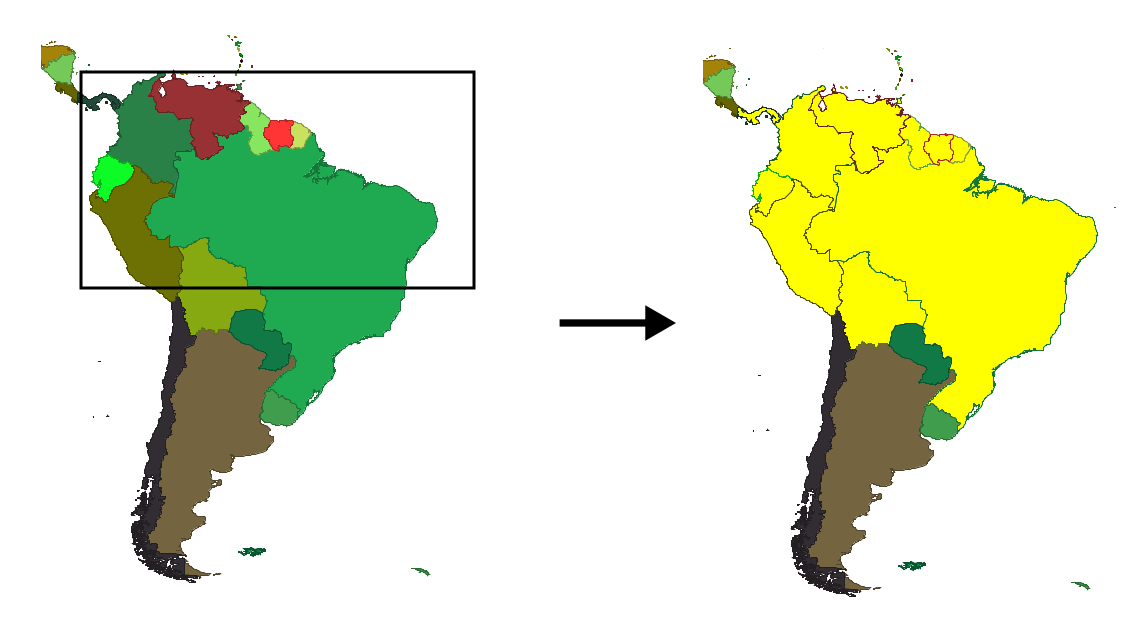
\includegraphics[width=\textwidth]{Bases_datos/Seleccion_rectangulo.png}
\caption{\small Una consulta sencilla mediante la definici�n gr�fica de un rect�ngulo. Todas las entidades dentro de este son el resultado de la consulta y quedan seleccionadas en el SIG.}
\label{Fig:Seleccion} 
\end{figure}


Una consulta nos vale tambi�n para extraer informaci�n de una base de datos de acuerdo a nuestras necesidades, y para crear posteriormente y a partir de dicha informaci�n una nueva capa. Esta operaci�n es �til cuando la base de datos de la que disponemos es muy voluminosa y solo resulta de inter�s para nuestro trabajo una parte de ella. Puede tratarse de una parte en el sentido espacial (la base de datos contiene datos a nivel mundial y se quiere trabajar a nivel estatal), en el sentido tem�tico (la base de datos contiene mucha informaci�n de cada entidad y solo interesan algunos campos), o en una combinaci�n de ambas. Para extraer dicha parte y trabajar �nicamente con ella, utilizaremos una consulta.

Veamos algunos ejemplos de consultas. Sea  una capa con los distintos pa�ses del mundo y una serie de valores econ�micos y sociales asociados a cada uno de ellos. Consideremos las siguientes preguntas:

\begin{itemize}
 \item �Qu� pa�ses tienen un Producto Interior Bruto mayor que el de Espa�a?
\item �Qu� pa�ses han experimentado un crecimiento econ�mico en el �ltimo a�o?
\item �Cu�ntos pa�ses tienen m�s de 200 millones de habitantes? 
\end{itemize}

En todos estos casos estamos haciendo referencia a pa�ses, los cuales, como sabemos, estar�n asociados a elementos geom�tricos que definan sus propiedades espaciales, es decir, a una componente espacial. Esta componente es la que permite que, adem�s de poder plantear las consultas anteriores, podamos representar cada pa�s en la pantalla y visualizarlo, o saber cu�les de ellos se encuentran en el hemisferio norte (esta ser�a una consulta espacial, de las que m�s adelante en este mismo cap�tulo veremos).

Sin embargo, cuando realizamos consultas como las tres anteriores, no acudimos para nada a la componente espacial. Consultas como estas podr�an resolverse si en lugar de una capa dentro de un SIG tuvi�ramos, por ejemplo, un simple anuario estad�stico lleno de tablas con datos correspondientes a cada pa�s. 

Las consultas pueden incluir varios criterios en una sola pregunta. Por ejemplo:

\begin{itemize}
 \item �Qu� pa�ses de la zona euro tienen m�s de 40 millones de habitantes?
\item �En qu� pa�ses de habla inglesa aument� la poblaci�n durante el �ltimo a�o?
\end{itemize}

Para expresar esas consultas se han de incluir elementos de la denominada \textbf{l�gica booleana}\footnote{Denominada as� por el matem�tico irland�s George Boole(1815, 1864)}. Esta implica el uso de \textbf{operadores l�gicos}, mediante los cuales se reescribir�an las consultas anteriores de la siguiente manera:

\begin{itemize}
 \item �Qu� pa�ses tienen como moneda el euro \emph{y} a la vez tienen m�s de 40 millones de habitantes?
\item �Que pa�ses hablan ingl�s \emph{y} sufrieron un aumento de poblaci�n durante el �ltimo a�o?
\end{itemize}

Los lenguajes de consulta que se emplean para transmitir estas operaciones a un SGBD, permiten el uso de tales operadores para formular consultas.

Si el SGBD es de tipo espacial y \emph{entiende} que algunas de las columnas de una tabla continene informacion espacial (es decir, que cada entidad no solo tiene informacion tem�tica), pueden plantearse consultas que hacen uso de esta, tales como las siguientes.

\begin{itemize}
\item �Qu� pa�ses comparten frontera con Alemania?
\item �Cu�ntos pa�ses se encuentran completamente en el hemisferio sur?
\item �Qu� pa�ses est�n a menos de 2000 km de Espa�a?
\end{itemize}

Para dar respuesta a esas cuestiones, basta analizar la componente espacial y no necesitamos para nada los datos con los que hemos trabajado anteriormente. Son consultas puramente espaciales. Aunque estas consultas ampl�an lo que ya conocemos, en realidad no abren ninguna nueva v�a de estudio de los datos geogr�ficos. Son consultas a las que podr�amos responder utilizando un mero mapa impreso, sin aprovechar el hecho de que dentro de un SIG las componentes espacial y tem�tica se hallan �ntimamente vinculadas. La verdadera potencia de las consultas espaciales la encontramos en la combinaci�n de estas consultas sobre la componente espacial y las que vimos anteriormente sobre la componente tem�tica. As�, se pueden plantear, por ejemplo, cuestiones como:

\begin{itemize}
 \item �Qu� pa�ses del hemisferio norte tiene una densidad de poblaci�n mayor que la de Per�?
\item �Cu�ntos pa�ses con m�s de 10 millones de habitantes se encuentran a menos de 1000 km de la frontera de Rusia?
\end{itemize}

Estas consultas incorporan elementos que hacen necesario acudir a la tabla de atributos, y otros que requieren analizar la componente espacial, estudiando las relaciones espaciales y topol�gicas de las geometr�as asociadas. 

Las consultas pueden incluir \textbf{varias capas}. Por ejemplo, si ademas de la capa de pa�ses disponemos de una capa de r�os del mundo, podr�amos responder a la pregunta \emph{�qu� pa�ses atraviesa el Nilo?}


Igualmente, las uniones entre tablas que hemos visto para el caso de la componente tem�tica pueden establecerse mediante un criterio espacial. Se tiene as� una \textbf{uni�n espacial}.

Un ejemplo muy sencillo de uni�n espacial es el que encontramos si combinamos la capa de pa�ses del mundo que venimos utilizando con una capa de ciudades del mundo. Podemos unir a la tabla de esta segunda capa todos los valores que caracterizan al pa�s al que pertenece cada ciudad. Si existe un campo com�n entre ambas tablas de atributos (por ejemplo, el nombre del pa�s), esto servir�a para efectuar esta uni�n. No obstante, esto no es necesario, ya que existe otro elemento com�n que no se encuentra almacenado dentro de la tabla, pero que puede tomarse de la componente espacial: toda ciudad debe estar situada dentro de los l�mites del pa�s al que pertenece. Esto sirve para establecer la relaci�n entre las tablas, y cada ciudad debe relacionarse con aquella entidad dentro de cuya geometr�a se encuentre el punto que la representa.



\subsection{�ndices espaciales}
\label{Indices_espaciales}


Si realizamos una consulta a una base de datos, el resultado es un subconjunto de esta con los elementos que cumplen el criterio expresado en la consulta. Si se implementa de forma \emph{directa} dicha consulta, esta operaci�n implica comprobar todos los elementos de la base de datos y ver cu�les son los que cumplen con el citado criterio. Teniendo en cuenta que una base de datos puede tener un gran tama�o, esta forma de proceder no es la �ptima.

Los �ndices nos permiten \emph{alcanzar} los elementos que constituyen la respuesta a nuestra consulta, haci�ndolo de la forma m�s r�pida y llegando hasta ellos sin tener que pasar por todos los restantes.

Un ejemplo f�cil de entender es el de una gu�a telef�nica en la que los nombre est�n ordenados alfab�ticamente. Gracias a ese orden y a que se conoce el alfabeto, se puede buscar rapidamente un nombre sin necesidad de leer todos ellos.

Al utilizar una base de datos, si no disponemos de un �ndice deberemos recorrer toda ella para dar respuesta a nuestras consultas. No sabemos \emph{d�nde} buscar las respuestas a nuestras consultas, del mismo modo que si en una guia telef�nica no supi�ramos que carece de sentido buscar en la letra F el n�mero telef�nico del se�or P�rez.

Ademas de �ndices para datos de tipo num�rico o texto, en los que resulta obvio establecer un orden natural, en el �mbito de los SIG tienen importancia los denominados \textbf{�ndices especiales}. Aunque sus fundamentos te�ricos son distintos, el concepto es similar al de �ndices de bases de datos no espaciales: elementos que permiten optimizar las consultas mediante una correcta estructuraci�n de los datos, en particular en este caso de su componente espacial.

Puede enterderse la idea de un �ndice espacial mediante un sencillo ejemplo de c�mo empleamos ideas parecidas a los �ndices espaciales de forma natural cuando tratamos de resolver una consulta espacial sin la ayuda de un SIG. Supongamos que tenemos nuestro mapa de pa�ses del mundo y queremos averiguar qu� pa�ses tienen su frontera a menos de 3000 kil�metros de la frontera de Espa�a. �C�mo operar�amos de manera natural para dar respuesta a esta consulta?

La soluci�n m�s inmediata es medir la distancia entre Espa�a y todos los pa�ses restantes, y despu�s tomar aquellos que hayan arrojado un resultado de distancia menor a 3000. La operaci�n dar�a el resultado esperado, pero implicar�a un gran n�mero de mediciones, y no ser�a una forma �ptima de operar. M�s probable es que no efectuemos mediciones con los pa�ses de Am�rica, pues un conocimiento b�sico de geograf�a basta para saber que todos ellos se encuentran a m�s de 3000 kil�metros. No sabemos exactamente a qu� distancia se encuentran, pero sabemos que no van a cumplir el criterio establecido en la consulta. 

Ese conocimiento b�sico de geograf�a que tenemos es en realidad una especie de �ndice espacial. No sirve para saber las distancias exactas ni resolver la consulta por completo, pero sirve para dar una aproximaci�n y facilitar el trabajo. Descartamos un buen numero de pa�ses de forma casi inmediata, y luego solo realizamos las operaciones costosas (la medici�n) con un subconjunto del total. 

De modo similar, los �ndices espaciales nos permiten obtener resultados en un �rea concreta sin necesidad de analizar todo el espacio ocupado por el total de los datos. Gracias a ello, hacen las consultas mas efectivas y permiten trabajar con grandes vol�menes de datos.

Los �ndices espaciales se almacenan junto con los datos a los que hacen referencia, bien en ficheros adicionales o dentro de la propia base de datos, en case de utilizarse una. Los SGBD espaciales tienen capacidades para calcular estos �ndices espaciales y almacenarlos en la base de datos, recurriendo a ellos cuando se realiza una consulta que requiera su uso.


\pagestyle{empty}
%\include{Datos/Metadatos/Metadatos}


%\pagestyle{empty}
\graphicspath{{Analisis/}}
\part{El analisis}
\label{Procesos}


\chapter{An�lisis espacial. Fundamentos}
\label{Introduccion_procesos}


\pagestyle{fancy}

El an�lisis espacial es una de las tareas fundamentales sin las cuales el concepto de SIG no alcanza su verdadero significado. 

El an�lisis espacial es el \textbf{estudio cuantitativo de aquellos fen�menos que se manifiestan en el espacio}. Ello indica una importancia clave de la posici�n, la superficie, la distancia y la interacci�n a trav�s del propio espacio. 

Ejemplos de an�lisis que realizamos con cartograf�a fuera de un SIG son el buscar en un mapa d�nde se sit�a el pico m�s alto, ver la elevaci�n concreta a la que se encuentra un elemento dado tal como una poblaci�n, o planificar una jornada tur�stica viendo qu� lugares de inter�s podemos visitar o c�mo llegar desde uno a otro de estos lugares haci�ndolo por las mejores carreteras o de la forma m�s r�pida. Estas actividades habituales son ejemplos de an�lisis geogr�ficos que podemos igualmente realizar dentro de un SIG.

Mediante el an�lisis podemos generar nuevos datos que pueden ser \textbf{nuevas capas de datos geogr�ficos, tablas de datos, valores escalares} o \textbf{vectores}.

En ocasiones, los resultados expresan \textbf{la misma variable} que el dato de partida (por ejemplo, el c�lculo de una media), y en otros las variables de entrada y salida son \textbf{distintas} (por ejemplo, si a partir de una capa de elevaciones calculamos una de pendientes).

Asimismo, todo an�lisis espacial parte de un conjunto de datos espaciales, pudiendo estos ser \textbf{de un �nico tipo, o de varios distintos} que se combinan en un procedimiento concreto. Por ejemplo, en el caso de calcular la localizaci�n del punto m�s alto, el resultado es una sencilla coordenada, y tan solo se utiliza la variable elevaci�n. En el caso de la altura media de una ciudad, se utilizan dos entradas: por un lado, la elevaci�n, y por otro, el emplazamiento de la ciudad. Aunque un mapa cl�sico contiene toda esa informaci�n en una �nica hoja, en realidad son dos elementos distintos combinados a la hora de representarlos. En t�rminos m�s acordes con un SIG, podemos decir que tenemos dos capas distintas que utilizamos como entradas.

El an�lisis dentro un SIG nos permite tanto formular como responder a cuestiones. Estas cuestiones pueden ser:

\begin{itemize}
 \item Relativas a posici�n y extensi�n
\item Relativas a la forma y distribuci�n
\item Relativas a la asociaci�n espacial
\item Relativas a la interacci�n espacial
\item Relativas a la variaci�n espacial
\end{itemize}

Algunos ejemplos de an�lisis geogr�fico son los siguientes.

\begin{itemize}
\item \textbf{Consulta espacial}. Vimos las consultas en detalle dentro del cap�tulo dedicado a las bases de datos.

\item \textbf{An�lisis topol�gico}. Pueden plantearse consultas referidas no solo a la posici�n de los elementos geogr�ficos, sino a la \textbf{relaci�n con otros elementos}. La existencia de topolog�a puede emplearse para la realizaci�n de consultas que respondan a cuestiones como:

\subitem �C�mo llegar desde mi posici�n actual hasta una coordenada concreta por la red viaria existente?

\subitem �Qu� comunidades aut�nomas comparten l�mite con Madrid?

\item \textbf{Medici�n}. La existencia de una referencia espacial para cada uno de los elementos con los que trabajamos en el an�lisis dentro de un SIG hace que podamos \textbf{cuantificar} otra serie de par�metros tambi�n espaciales. Entre las mediciones m�s b�sicas, encontramos las distancias, �reas, per�metros o factores de forma. Mas elaboradas, encontramos otras como pendientes o indices derivados de medidas simples.


\item \textbf{Combinaci�n}. Uno de los procedimientos m�s habituales y m�s caracter�sticos dentro del uso de un SIG es la \textbf{combinaci�n o superposici�n} de varias capas de informaci�n. La propia estructura de la informaci�n geogr�fica en capas facilita notablemente estos procedimientos y convierte a los SIG en plataformas ideales para llevar a cabo an�lisis donde se combina informaci�n sobre diversas variables.



\item \textbf{Transformaciones}. Podemos englobar dentro de este grupo una amplia serie de procedimientos que modifican los elementos de entrada de diversas formas. Entre los m�s habituales, encontramos la \textbf{transformaci�n de coordenadas}, la \textbf{simplificaci�n de geometr�as}, o la \textbf{creaci�n de �reas de influencia} o la \textbf{reclasificaci�n de valores}. Estas transformaci�n pueden afectar tanto a la componente espacial como a la componente tem�tica del dato. 

\item \textbf{An�lisis de superficies}. El an�lisis de superficies es uno de los m�s potentes de cuantos encontramos en un SIG. Desde par�metros b�sicos como la \textbf{pendiente} o la \textbf{orientaci�n} hasta par�metros morfom�tricos muy espec�ficos, pasando por todas las herramientas del \textbf{an�lisis hidrol�gico}, la bater�a de operaciones disponibles es muy amplia. 

\item \textbf{Estad�stica descriptiva}. Los elementos de la estad�stica cl�sica tienen sus equivalentes en los datos espaciales, y nos permiten \textbf{calificar cuantitativamente} los datos con los que trabajamos. Se incluyen aqu� descriptores de centralidad y dispersi�n, de dependencia espacial o el estudio de patrones espaciales, entre otros muchos. Estos pueden a su vez usarse para el contraste de hip�tesis que contengan una cierta componente espacial.

Por ejemplo, estos estad�sticos nos permiten dar respuesta a cuestiones del tipo

\subitem �Es constante la media de altura a lo largo de toda la geograf�a de mi pa�s?

\subitem �Existe alguna direcci�n predominante en los movimientos de individuos de una especie o se desplazan err�ticamente?

\item \textbf{Inferencia}. Otro an�lisis estad�stico de gran importancia en los SIG es el que permite inferir comportamientos de las distintas variables y estudiar, por ejemplo, la forma en que estas van a evolucionar a lo largo del tiempo.

El establecimiento de modelos de cambio y variaci�n representa una de las herramientas m�s actuales en el campo de los SIG, y un campo en abundante desarrollo.

\item \textbf{Toma de decisiones y optimizaci�n}. La estructura de la informaci�n geogr�fica en capas dentro de un SIG, favorable como ya vimos para la superposici�n de capas, lo es igualmente para estudiar de forma combinada los efectos de distintos factores. Este estudio nos permite luego responder a cuestiones como, por ejemplo,

\subitem �Cu�l es el mejor lugar para emplazar una nueva construcci�n en funci�n de su impacto sobre el medio?

\subitem �D�nde situar un nuevo hospital para que el servicio en la comarca mejore lo m�ximo posible?

\item \textbf{Modelizaci�n}. La creaci�n de modelos espaciales dentro de un SIG es una tarea a�n pendiente de mucho desarrollo. No obstante, existe un gran n�mero de modelos en los m�s diversos campos, y la arquitectura de datos y procesos de los SIG es propicia para la implementaci�n de otros nuevos.
\end{itemize}

\section{Particularidades de los datos espaciales para su an�lisis}
\label{Analisis_espacial}


Las caracter�sticas propias de los datos espaciales dotan a estos de una \textbf{gran potencialidad} de an�lisis, al tiempo que \textbf{condicionan o limitan} otras operaciones. Algunas de estas caracter�sticas representan problemas que han de tenerse presentes en el an�lisis; otros son simplemente conceptos b�sicos que deben conocerse pero no han de implicar necesariamente una dificultad asociada.

\subsection{Escala}
\label{Escala_analisis}

A la hora de estudiar la informaci�n geogr�fica, podemos hacerlo a \textbf{distintos niveles} y, dependiendo del nivel elegido, los resultados ser�n de una u otra naturaleza. Debido a esto, adem�s de considerar la escala cartogr�fica para la representaci�n y gesti�n de datos en un SIG, es necesario considerar la \textbf{escala de an�lisis}.

La escala de an�lisis depende \textbf{del dato en s�} (precisi�n, tipo, etc.), as� como del \textbf{an�lisis que se va a realizar} con �l.

Como se muestra en la figura \ref{Fig:Escalas_formas_terreno}, si para definir las formas de relieve en un punto dado lo hacemos considerando dicho punto y los valores de elevaci�n a su alrededor, la caracterizaci�n que hagamos var�a en funci�n de la dimensi�n de esa zona alrededor (que es la que define la escala de an�lisis). Para valores peque�os de dicha zona de an�lisis, el punto analizado puede definirse como una cima, mientras que aumentando la escala de an�lisis se advierte que el punto se sit�a en el fondo de un valle.

\begin{figure}[h]   
\centering
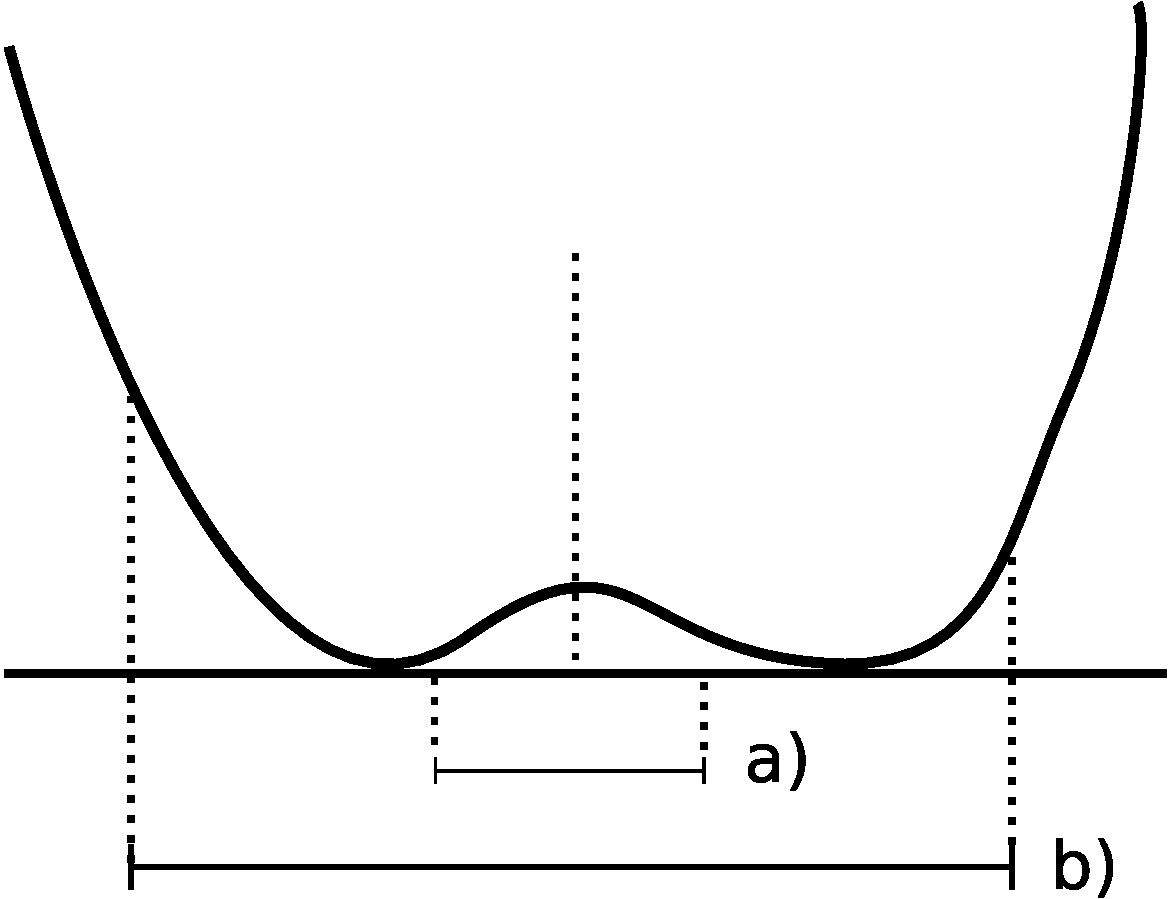
\includegraphics[width= .45\mycolumnwidth]{Analisis_espacial/Escalas_formas_terreno.pdf}
\caption{\small Dependiendo de la escala de an�lisis, un mismo relieve puede ser caracterizado como cima (a) o fondo de valle (b)}
\label{Fig:Escalas_formas_terreno} 
\end{figure}

Por tanto, debemos observar el relieve desde la distancia correcta a la cual la informaci�n que nos proporciona es la m�s adecuada para un an�lisis dado. Adem�s de existir una escala de mayor relevancia para un an�lisis concreto,  es de inter�s el trabajar a \textbf{m�ltiples escalas} y combinar los resultados.

Otro ejemplo de c�mo la escala de an�lisis condiciona los resultados obtenidos lo encontramos en el caso de efectuar \textbf{mediciones}. Como puede verse en la figura \ref{Fig:Medida_linea_fractal}, la unidad de medida empleada provoca que se obtengan resultados distintos. 

\begin{figure}[h]   
\centering
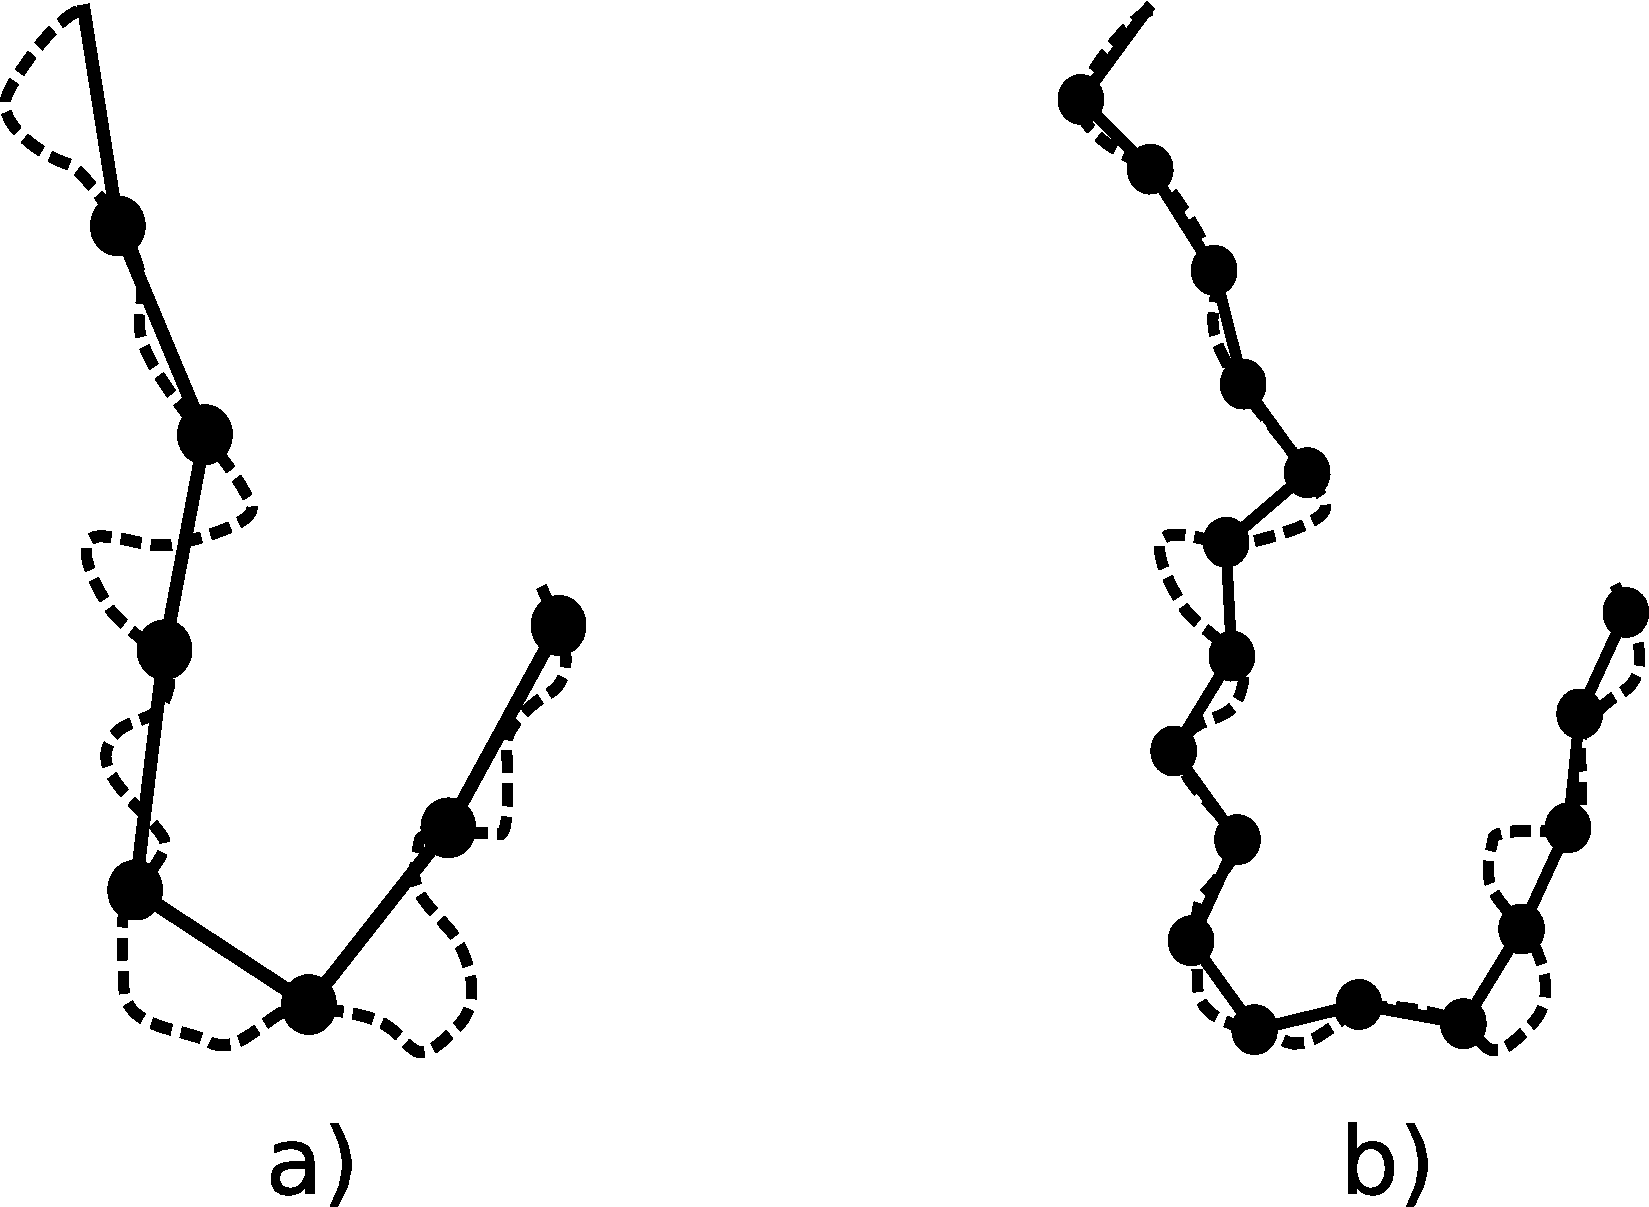
\includegraphics[width= .45\mycolumnwidth]{Analisis_espacial/Medida_linea_fractal.pdf}
\caption{\small La unidad de medida empleada modifica el resultado obtenido.}
\label{Fig:Medida_linea_fractal} 
\end{figure}

La uni�n del valor resultante con la escala a la que se ha obtenido tiene en conjunto pleno significado, pero ese valor por s� mismo carece de dicho significado. 

El concepto de \textbf{fractal} tiene una implicaci�n directa en este hecho.

El propio \textbf{formato de almacenamiento} condiciona el efecto de la escala, ya que puede imponer l�mites. Tal es el caso cuando se trabaja con capas raster, en las que el \textbf{tama�o de celda} delimita la precisi�n que puede obtenerse en el an�lisis.

\subsection{El Problema de la Unidad de �rea Modificable}
\label{MAUP}

Muchas de las variables con las que trabajamos dentro de un SIG \textbf{no pueden medirse de forma puntual}, y por ello han de \textbf{estudiarse para un �rea dada}. Ejemplos de este tipo de variables son el porcentaje de poblaci�n en un rango de edad determinado o la densidad media de poblaci�n.

Las �reas que se definen para poder trabajar con las variables de esta �ndole son \textbf{esencialmente arbitrarias}, tales como pa�ses, regiones o distritos, que se establece sin ning�n criterio propio del an�lisis espacial. La utilizaci�n de una u otra unidad \textbf{altera los resultados} extra�dos de las variables estudiadas.

Este problema, por tener relaci�n con la elecci�n de la unidad de agregaci�n de la informaci�n, se conoce como \emph{Problema de la Unidad de �rea Modificable}(PUAM).


Un problema particular relacionado con el PUAM es la denominada \textbf{falacia ecol�gica}, que consiste en asumir que los valores calculados para una unidad de �rea pueden aplicarse a los individuos de la poblaci�n existente en dicha �rea. S�lo en el caso de que exista una completa homogeneidad para la variable analizada, lo cual raramente sucede, la anterior suposici�n ser�a cierta.

\subsection{Autocorrelaci�n espacial} 
\label{Autocorrelacion_espacial}

Se denomina \textbf{autocorrelaci�n espacial} a la existencia de una \textbf{correlaci�n de la variable consigo misma}, de tal modo que los valores de esta variable en un punto guardan relaci�n directa con los de esa misma variable en otros puntos cercanos. Por ejemplo, en el caso de medirse la temperatura, los puntos cerca de un foco de calor tendr�n una temperatura mayor que aquellos cerca de focos fr�os. Si estudiamos la distribuci�n de una enfermedad infecciosa, es m�s probable que los casos se encuentren agrupados, de forma que la presencia de un alto n�mero de casos implique tambi�n una alta incidencia en poblaciones cercanas.

Otra forma de expresar la autocorrelaci�n espacial es mediante la conocida como \textbf{Primera Ley Geogr�fica de Tobler}, que establece que <<todo est� relacionado con todo, pero las cosas pr�ximas entre s� est�n m�s relacionadas que las distantes>>.

La autocorrelaci�n espacial, tal y como se ha descrito antes, es \textbf{positiva}. Puede, no obstante, existir una \emph{autocorrelaci�n espacial negativa}, si los valores altos se rodean de valores bajos y viceversa.

En caso de no existir ning�n tipo de autocorrelaci�n espacial, se tiene que los datos recogidos en una serie de puntos son \textbf{independientes entre s�} y no se afectan mutuamente, sin que tenga influencia de la distancia.

La figura \ref{Fig:Autocorrelacion_espacial} muestra unas sencillas capas r�ster en las que se presentan los tres tipos de autocorrelaci�n espacial anteriores.

\begin{figure}[!hbt]   
\centering
\includegraphics[width=\textwidth]{Analisis_espacial/Autocorrelacion_espacial.png}
\caption{\small a) Autocorrelaci�n espacial positiva. b) Autocorrelaci�n espacial negativa. c) Ausencia de autocorrelaci�n espacial (independencia)}
\label{Fig:Autocorrelacion_espacial} 
\end{figure}

Las consecuencias de la existencia de autocorrelaci�n espacial son numerosas y de gran importancia.

Por una parte, muchos de los an�lisis estad�sticos suponen la \textbf{independencia de la variable}. Puesto que existe una dependencia de la componente espacial, ser� necesario para obtener resultados correctos introducir dicha componente espacial como una variable m�s. 

Algo similar sucede cuando los datos presentan alguna \textbf{tendencia espacial} (los valores de una variable est�n relacionados con sus propias coordenadas geogr�ficas), ya que esto tambien invalida el supuesto de la independencia de los datos.

Existiendo autocorrelaci�n espacial, y siendo esta positiva, la \textbf{inferencia estad�stica es menos eficaz} que si se cuenta con un n�mero igual de observaciones de una variable independiente. 

La autocorrelaci�n espacial no es, no obstante, un elemento que siempre tenga consecuencias negativas. Puesto que los puntos cercanos a uno dado guardan relaci�n con este, la autocorrelaci�n puede aprovecharse para \textbf{estimar valores} en un punto cualquiera si conocemos los valores en puntos cercanos. Este es el fundamento de los \textbf{m�todos de interpolaci�n}


\subsection{Existencia de estructura}

Tanto la disposici�n de los datos como las propiedades de la variable estudiada (por ejemplo, la propia autocorrelaci�n espacial como propiedad intr�nseca) exhiben una estructura determinada. Esta estructura puede condicionar los resultados del an�lisis y tener influencia sobre estos.

Los dos principales conceptos estad�sticos que definen la estructura espacial de los datos son la \textbf{estacionaridad} y la \textbf{isotrop�a}. La estacionaridad indica que el proceso es \textbf{invariante a la traslaci�n}. Es decir, que las propiedades son constantes en el espacio y no existe tendencia alguna. La isotrop�a indica que el proceso es \textbf{invariante a la rotaci�n} y tiene lugar del mismo modo en todas direcciones. 


\subsection{Efectos de borde}
\label{EfectoBorde}

Las zonas que estudiamos dentro de todo an�lisis espacial \textbf{tienen unos l�mites establecidos}. Estos l�mites vienen definidos de forma artificial ---el l�mite de la fotograf�a a�rea de la que disponemos, por ejemplo--- o bien de forma natural ---si estudiamos un bosque junto a un pantano, el bosque encuentra su l�mite al borde de este �ltimo---. La presencia de estos bordes \textbf{distorsiona el resultado de los an�lisis}, en especial para aquellos par�metros no puntuales que requieren la definici�n de un area de estudio (densidades, etc., como ya vimos para el caso del PUAM)

La figura \ref{Fig:Efecto_borde} muestra un ejemplo de efecto de borde.

\begin{figure}[h]   
\centering
\includegraphics[width=.35\columnwidth]{Analisis_espacial/Efecto_borde.pdf}
\caption{\small Representaci�n del efecto borde y c�mo este afecta en mayor o menor medida en funci�n de la escala de an�lisis. Las zonas en trazo continuo no se ven afectadas. Las zonas en trazo punteado est�n afectadas de efecto de borde en diferente grado.}
\label{Fig:Efecto_borde} 
\end{figure}

En algunos casos, el efecto de borde no se manifiesta �nicamente para puntos cercanos a dicho borde, sino para \textbf{todos aquellos relacionados o conectados} con �l seg�n un determinado criterio, con independencia de su distancia a este.


\pagestyle{empty}
%
\chapter{Conceptos b�sicos para el an�lisis espacial} \label{Analisis_espacial}



\bigskip

\begin{intro}
Para proceder al an�lisis de los datos espaciales, deben conocerse antes las particularidades de estos. Algunas caracter�sticas propias de los datos espaciales hacen que, entre otras cosas, no sean aplicables algunos elementos de la estad�stica no espacial. Otras condicionan buena parte de las formulaciones que operan sobre ellos, y que iremos viendo en los sucesivos cap�tulos. Por tanto, abordar el estudio de estas formulaciones no se ha de hacer sin antes tratar con algo m�s de detalle las propiedades inherentes al dato espacial en lo que a su disposici�n para el an�lisis respecta.

Junto a esto, se presentan en este cap�tulo algunos conceptos fundamentales sobre geometr�a del plano y el espacio, y sobre las distintas relaciones entre entidades espaciales. Todos ellos son la base para crear an�lisis m�s complejos sobre datos espaciales. Unas nociones b�sicas de matem�ticas son necesarias para poder comprender estas ideas.
\end{intro}


\section{Introducci�n}
\pagestyle{fancy}

Trabajar con datos espaciales tiene una serie de implicaciones que han de considerarse con detenimiento antes de llevar a cabo cualquier an�lisis. A lo largo de esta parte del libro veremos formas muy distintas de analizar los datos espaciales para obtener resultados de �ndole variada, y todas ellas tienen en com�n el hecho de trabajar sobre este tipo particular de datos. Conocer en profundidad el dato espacial es, por tanto, imprescindible, no solo en lo relativo a su forma, su manejo y su almacenamiento ---que ya fue visto en la parte correspondiente--- sino tambi�n en lo referente a su an�lisis y c�mo ha de tratarse e interpretarse la informaci�n que contiene ---que lo veremos en el presente cap�tulo---.

Entendemos por dato espacial todo aquel que tiene asociada una referencia geogr�fica, de tal modo que podemos localizar exactamente \emph{d�nde} sucede dentro de un mapa \cite{Haining2003Cambridge}. Dentro de esta definici�n se incluyen datos de campos (superficies) o datos asociados a objetos como puntos, l�neas o pol�gonos. Es decir, todo cuanto puede recogerse seg�n los distintos modelos de representaci�n que ya hemos visto con anterioridad.

El objetivo de este cap�tulo es m�ltiple. Por una parte, presentar las principales particularidades de los datos espaciales, as� como la formas de tener estas en cuenta a la hora del an�lisis. Por otra, estimular un correcto razonamiento espacial y un entendimiento adecuado tanto de las limitaciones como de la potencialidad de los datos espaciales como fuente del an�lisis geogr�fico. Y por �ltimo, presentar algunos de los fundamentos te�ricos sobre los cuales se crean despu�s todas las metodolog�as de an�lisis, las estad�sticas espaciales, y los algoritmos que se detallar�n en los cap�tulos sucesivos. 

Estos fundamentos incluyen algunas nociones b�sicas sobre matem�tica del plano y el espacio, y conceptos sobre las posibles relaciones existentes entre objetos geogr�ficos.

\section{Particularidades de los datos espaciales}

Considerar que el dato espacial es un dato cualquiera sin ninguna peculiaridad supone no realizar sobre �l un an�lisis �ptimo. Las caracter�sticas propias de los datos espaciales dotan a estos de una gran potencialidad de an�lisis, al tiempo que condicionan o limitan otras operaciones. Asimismo, estas particularidades son el origen de una gran parte de los retos a�n existentes dentro del an�lisis geogr�fico, y por sus implicaciones directas no pueden desestimarse sin m�s. Su conocimiento es, por tanto, imprescindible para todo tipo de an�lisis espacial.

El car�cter especial del dato espacial deriva de la existencia de posici�n. Esta posici�n se ha de entender tanto en t�rminos absolutos (posici�n de una entidad en el espacio expresada por sus coordenadas) como relativos (relaci�n con otras entidades tambi�n en dicho espacio). Las consecuencias de que todo dato espacial se halle por definici�n localizado a trav�s de coordenadas son diversas, y deben enfocarse desde los distintos puntos de vista del an�lisis espacial. A continuaci�n veremos los puntos m�s relevantes que deben considerarse a la hora de tratar con datos espaciales.

Algunos de estos puntos representan problemas que han de tenerse presentes en el an�lisis. Otros son simplemente conceptos b�sicos que deben conocerse pero no han de implicar necesariamente una dificultad asociada.

\subsection{Escala}
\label{Escala_analisis}

En el apartado \ref{Escala} vimos con detalle el concepto de escala cartogr�fica, y c�mo este se aplica de igual modo a la representaci�n y gesti�n dentro de un SIG. Existe, adem�s, otra forma de considerar la escala, y que resulta de especial inter�s para los contenidos de esta parte: la escala de an�lisis. \index{Escala!de an�lisis}

A la hora de estudiar la informaci�n geogr�fica, podemos hacerlo a distintos niveles y, dependiendo del nivel elegido, los resultados ser�n de una u otra naturaleza. Esto se manifiesta en las estructuras espaciales (v�ase m�s adelante en esta misma secci�n), que condicionan los valores que se derivan de sus an�lisis a trav�s de las distintas formulaciones de an�lisis. Este hecho es f�cil verlo con algunos ejemplos, que nos permitir�n comprobar c�mo a distintas escalas los datos geogr�ficos tienen caracter�sticas distintas. 

Por ejemplo, sea el conjunto de puntos de la figura \ref{Fig:Estructura_escalas}. En el ejemplo a) se ve que los puntos se agrupan en conglomerados en zonas concretas del espacio. Esto es lo que denominaremos una estructura \emph{agregada}. Sin embargo, si nos acercamos y solo enfocamos uno de dichos grupos, el de la parte superior izquierda ---ejemplo b)---, la estructura que vemos claramente no responde a una estructura agregada, sino que los puntos se disponen m�s o menos equiespaciados. Es lo que se conoce como estructura \emph{regular}. Dependiendo de a qu� escala observemos y analicemos la estructura espacial del conjunto de puntos, esta resulta de un tipo o de otro.

\index{Estructura!regular}\index{Estructura!agregada}

\begin{figure}[h]   
\centering
\includegraphics[width= .55\mycolumnwidth]{Analisis_espacial/Estructura_escalas.pdf}
\caption{\small Dependiendo de la escala de an�lisis, la estructura de un conjunto de puntos puede ser distinta.}
\label{Fig:Estructura_escalas} 
\end{figure}

La escala de an�lisis debe ir inseparablemente relacionada con el fen�meno que pretendemos analizar, ya que es esta la que le da sentido. Supongamos el caso de llevar a cabo un an�lisis del relieve. Dependiendo de a qu� escala observemos dicho relieve, la imagen que obtenemos es muy distinta. A un nivel global, distinguimos las grandes cadenas monta�osas, y el resto del relieve aparece m�s o menos llano. Si nos acercamos a alguna de esas zonas llanas, se aprecia un relieve que antes no percib�amos, con ondulaciones y accidentes orogr�ficos de menor entidad, que son suficientes para apreciarse a esta escala, pero no a la escala global anterior. Siguiendo este proceso, podemos ir acerc�ndonos progresivamente hasta que incluso un peque�o grano de arena constituya un relieve notable.

Si vamos a llevar a cabo un estudio de c�mo el relieve influye en los movimientos de las masas de aire a nivel de todo el planeta, no tiene sentido estudiar las formas del relieve a este �ltimo nivel de m�ximo detalle. Como se muestra en la figura \ref{Fig:Escalas_formas_terreno}, si para definir las formas de relieve en un punto dado lo hacemos considerando dicho punto y los valores de elevaci�n a su alrededor, la caracterizaci�n que hagamos var�a en funci�n de la dimensi�n de esa zona alrededor (que es la que define la escala de an�lisis). Para valores peque�os de dicha zona de an�lisis, el punto analizado puede definirse como una cima, mientras que aumentando la escala de an�lisis se advierte que el punto se sit�a en el fondo de un valle.

\begin{figure}[h]   
\centering
\includegraphics[width= .45\mycolumnwidth]{Analisis_espacial/Escalas_formas_terreno.pdf}
\caption{\small Dependiendo de la escala de an�lisis, un mismo relieve puede ser caracterizado como cima (a) o fondo de valle (b)}
\label{Fig:Escalas_formas_terreno} 
\end{figure}

Por tanto, debemos observar el relieve desde la distancia correcta a la cual la informaci�n que nos proporciona es la m�s adecuada para un an�lisis dado. Adem�s de existir una escala de mayor relevancia para un an�lisis concreto, lo cierto es que el conjunto de todas las escalas de an�lisis contiene en su totalidad una informaci�n m�s amplia que la correspondiente a una �nica escala, y por tanto resulta de inter�s el trabajar a m�ltiples escalas y combinar los resultados.

Este enfoque de escalas m�ltiples es relevante tambi�n en relaci�n con los propios datos, independientemente de lo que representan. Es decir, independientemente de la escala y la dimensi�n <<real>>, y en relaci�n solo con la escala definida por el formato de los mismos. Por ejemplo, en el caso de im�genes, el uso de operadores a diferentes escalas (referida aqu� la escala al n�mero de p�xeles utilizados en el operador) es ventajoso para realizar ciertas operaciones tales como la detecci�n de bordes \cite{Rossenfeld1971IEEE}(v�ase \ref{DeteccionBordes}). Combinado esto con lo anterior, la importancia de la escala en el an�lisis espacial es de primer orden, y resulta necesaria su consideraci�n en todo momento.\index{Pixel}

Podemos ver m�s ejemplos de c�mo la escala de an�lisis condiciona los resultados obtenidos. Sup�ngase un elemento lineal tal como un camino o el contorno de una finca cuyo per�metro quiere medirse. Como puede verse en la figura \ref{Fig:Medida_linea_fractal}, la unidad de medida empleada provoca que se obtengan resultados distintos. Para medir la longitud de la l�nea utilizamos una unidad m�nima, que podemos asimilar a una especie de <<vara de medir>>. Todos los elementos de la l�nea que son menores que esa unidad m�nima no se recogen. En el caso a) se obtiene un resultado de siete unidades. Si reducimos a la mitad la unidad, cabe esperar que la longitud sea el doble. Sin embargo, obtenemos un total de 17 unidades, de forma que la proporci�n entre el tama�o de nuestra vara de medida y el n�mero de unidades resultante no se mantiene.

\begin{figure}[h]   
\centering
\includegraphics[width= .45\mycolumnwidth]{Analisis_espacial/Medida_linea_fractal.pdf}
\caption{\small La unidad de medida empleada modifica el resultado obtenido.}
\label{Fig:Medida_linea_fractal} 
\end{figure}

Cuando esto sucede, podemos afirmar que carece de fundamento trabajar con una medida <<absoluta>> de longitud (u otro par�metro estudiado que se comporte de igual manera, tal como el per�metro de un �rea de estudio), y que esto solo tiene sentido dentro de un contexto dado que defina la forma en que los resultados son medidos y operados. La uni�n de un valor resultante con la escala a la que se ha obtenido tiene en conjunto pleno significado, pero en casos como el anterior el valor resultante por s� mismo carece de dicho significado. Otra soluci�n es la definici�n de par�metros invariantes a la escala, que no se ven afectados por esta.

El concepto de \emph{fractal} tiene una implicaci�n directa en este hecho. Para saber m�s sobre fractales, la referencia cl�sica es \cite{Mandelbrot1982Freeman}. \index{Fractal}

Por �ltimo, y para concluir este apartado,  se�alar que las implicaciones de la escala para el an�lisis se incorporan incluso en la representaci�n y almacenamiento de los datos espaciales. As�, una ciudad puede definirse como un punto a una escala dada, y como un pol�gono si nos acercamos lo suficiente y estudiamos una porci�n concreta con m�s detalle. En funci�n de su uso, puede ser m�s conveniente tratar el elemento \emph{ciudad} de una u otra manera, lo cual tambi�n afecta al an�lisis del mismo.

En realidad, los conceptos \emph{punto} y \emph{l�nea} no existen como tales en el espacio geogr�fico. Un elemento tal como un cauce o una l�nea de alta tensi�n, que se recogen ambos en una capa vectorial como l�neas, en realidad tiene un grosor. Lo mismo sucede con los elementos puntuales. Un �rbol no es un punto, sino en todo caso un c�rculo. Por motivos de escala hacemos la abstracci�n de considerar puntos o l�neas, porque a la escala habitual dichos elementos (�rboles, caminos, etc.) pueden considerarse como tales.

Tambi�n el propio formato de almacenamiento condiciona el efecto de la escala. Para el caso de datos vectoriales, existe el l�mite impuesto por la imposibilidad de almacenar n�meros decimales de la precisi�n deseada. Es decir, la limitaci�n del m�nimo valor que puede almacenarse. No obstante, este l�mite es varios �rdenes de magnitud inferior al definido por la precisi�n de los instrumentos de medida, con lo que no es considerable.

Una situaci�n distinta es la que sucede con los datos r�ster, donde el tama�o de celda est� indirectamente condicionando una escala. La medici�n de �reas y distancias se encuentra influida por el tama�o elegido. Del mismo modo que no podemos recoger los detalles m�nimos de una curva al utilizar una vara de medir de mayor tama�o, en el caso de una capa r�ster, todo aquello que suceda en una escala inferior a la definida por el tama�o de celda queda ignorado. La espacial resoluci�n es, por tanto, un elemento directamente relacionado con los resultados del an�lisis cuando se utilizan datos r�ster.

\subsection{El \emph{Problema de la Unidad de �rea Modificable}}
\label{MAUP}

Uno de los problemas principales asociados al an�lisis de datos espaciales es el relacionado con la definici�n de unidades de an�lisis. Muchas de las variables con las que trabajamos dentro de un SIG no pueden medirse de forma puntual, y por ello han de estudiarse para un �rea dada. Ejemplos de este tipo de variables son el porcentaje de poblaci�n en un rango de edad determinado o la densidad media de poblaci�n.\index{Problema de la Unidad de �rea Modificable}

Las �reas que se definen para poder trabajar con las variables de esta �ndole son esencialmente arbitrarias. Por ejemplo, podemos estudiar el porcentaje de la poblaci�n dentro de un intervalo de edad a nivel de pa�s. La unidad \emph{pa�s} se establece sin ning�n criterio propio del an�lisis espacial, de igual modo que podr�a haberse realizado el mismo an�lisis a nivel de continente o de comarca, todas ellas divisiones por completo arbitrarias. No obstante, la utilizaci�n de una u otra unidad es problem�tica, ya que altera los resultados extra�dos de las variables estudiadas.

Este problema, por tener relaci�n con la elecci�n de la unidad de agregaci�n de la informaci�n, se conoce como \emph{Problema de la Unidad de �rea Modificable}(PUAM) \cite{Openshaw1983Geobooks} \footnote{\emph{Modifiable Areal Unit Problem, MAUP}}, y ha sido ampliamente estudiado en la literatura. Formalmente, puede definirse como <<un problema causado por la imposici�n de unidades artificiales de definici�n espacial en fen�menos geogr�ficos continuos, teniendo �sto como consecuencia la generaci�n de patrones artificiales>> \cite{Heywood1998Wesley}. Aunque no se trata de una cuesti�n de reciente descubrimiento, la aparici�n de los SIG y las mayores capacidades de an�lisis que estos han propiciado ha atra�do de nuevo el inter�s sobre el Problema de la Unidad de �rea Modificable. \index{Modifiable Areal Unit Problem}

Los efectos del PAUM se pueden dividir en dos componentes: uno relacionado con la escala y otro relacionado con la agregaci�n. El \emph{efecto de escala} describe la variaci�n de los resultados obtenidos en relaci�n con el n�mero de zonas en que se divide el total de la zona de estudio. Es decir, el tama�o de las unidades. Este efecto esta claramente relacionado con lo visto en el punto anterior.\index{Escala!efecto de}

Por su parte, el \emph{efecto de zonificaci�n} hace referencia a las diferencias que se producen cuando la informaci�n se agrega a una escala distinta. Por ejemplo, si se miden los datos de densidad de poblaci�n por t�rminos municipales, y posteriormente estos se agregan para presentarse por comunidades aut�nomas, ese cambio en la unidad de definici�n da lugar a diferencias en los valores resultantes. \index{Efecto!de escala}\index{de zonificaci�n}

Para darse cuenta de la importancia de este hecho, debe considerarse que una buena parte de la informaci�n geogr�fica que utilizamos en un SIG ha sido recogida originalmente a una escala distinta, y en ocasiones ha sufrido una agrupaci�n en unidades mayores por motivos de mera facilidad de manejo.

Ambos efectos, el de zonificaci�n y el de escala, no son independientes, sino que est�n �ntimamente relacionados.
La intensidad con que estos dos efectos afectan al an�lisis es variable, y existe asimismo una componente aleatoria. En l�neas generales, el uso de unidades peque�as implica que el n�mero de elementos contenidos en las mismas es menor y por lo tanto estad�sticamente menos fiable. En el extremo contrario, el uso de unidades grandes da valores estad�sticamente m�s fiables pero oculta la variaci�n que se produce dentro de las propias unidades.\cite{Nakaya2000EP}.

A pesar de tener una clara importancia en el an�lisis geogr�fico, las soluciones a la problem�tica que la definici�n de un �rea unitaria conlleva no son claras. Tradicionalmente se considera que se trata de un problema intratable. No obstante, algunos estudios \cite{Reynolds1998PhD} indican que existe un cierto grado de regularidad en los valores estad�sticos agregados, dependiente de la autocorrelaci�n espacial (ver siguiente punto) y la configuraci�n de la variable. 

Puede afirmarse que el Problema de la Unidad de �rea Modificable es a�n materia de amplio estudio, y el objeto de este estudio, que no es otro que el poder calcular los valores de los datos a la resoluci�n espacial original (es decir, sin que los efectos de zonificaci�n tengan relevancia), en caso de poder alcanzarse, requerir� un an�lisis sin duda complejo.

Un problema particular relacionado con el PUAM es la denominada \emph{falacia ecol�gica}\cite{Openshaw1983Geobooks}, que consiste en asumir que los valores calculados para una unidad de �rea pueden aplicarse a los individuos de la poblaci�n existente en dicha �rea. S�lo en el caso de que exista una completa homogeneidad para la variable analizada, lo cual muy raramente sucede, la anterior suposici�n ser�a cierta.\index{Falacia ecol�gica}

\subsection{Autocorrelaci�n espacial} 
\label{Autocorrelacion_espacial}

Sup�ngase que se estudian una serie de poblaciones cercanas en las cuales se mide el porcentaje de personas afectadas por una determinada enfermedad infecciosa. Cabe esperar que, puesto que los habitantes de esas poblaciones est�n relacionados entre s� de diversas formas, la distribuci�n de los valores recogidos obedezca en parte a la existencia de dichas relaciones. Por ejemplo, si en una poblaci�n contraen la enfermedad un n�mero dado de habitantes, es m�s factible que estos puedan contagiar a los de las poblaciones cercanas que a los de otros n�cleos m�s alejados.

Por lo anterior, es probable que alrededor de una poblaci�n con muchos casos de la enfermedad haya otras tambi�n con un elevado n�mero de afectados, mientras que una poblaci�n con pocos casos est� rodeada de otras tambi�n con escasa afecci�n. Un comportamiento similar lo encontrar�amos si midi�ramos la concentraci�n de un t�xico en distintos puntos de un embalse, ya que alrededor de un punto de alta concentraci�n no parece l�gico esperar concentraciones bajas.

Ejemplos como los anteriores cumplen lo que se conoce como \emph{Primera Ley Geogr�fica de Tobler} \cite{Tobler1970EcoGeo}, que establece que <<todo est� relacionado con todo, pero las cosas pr�ximas entre s� est�n m�s relacionadas que las distantes>>.\index{Primera ley geogr�fica de Tobler}

De modo m�s formal, el termino \emph{autocorrelaci�n espacial} hace referencia a lo reflejado en los ejemplos anteriores, es decir, a la existencia de una correlaci�n de la variable consigo misma, de tal modo que los valores de esta variable en un punto guardan relaci�n directa con los de esa misma variable en otros puntos cercanos.\index{Autocorrelaci�n espacial}

En el caso de la enfermedad infecciosa o la concentraci�n del producto t�xico, los valores altos suelen tener en su entorno valores tambi�n altos, y de modo similar sucede para valores bajos. Se dice que existe una \emph{autocorrelaci�n espacial positiva}.  Puede, no obstante, existir una \emph{autocorrelaci�n espacial negativa}, si los valores altos se rodean de valores bajos y viceversa.

En caso de no existir ning�n tipo de autocorrelaci�n espacial, se tiene que los datos recogidos en una serie de puntos son independientes entre s� y no se afectan mutuamente, si que tenga influencia de la distancia.

La figura \ref{Fig:Autocorrelacion_espacial} muestra unas sencillas capas r�ster en las que se presentan los tres tipos de autocorrelaci�n espacial anteriores.

\begin{figure}[!hbt]   
\centering
\includegraphics[width=\textwidth]{Analisis_espacial/Autocorrelacion_espacial.png}
\caption{\small a) Autocorrelaci�n espacial positiva. b) Autocorrelaci�n espacial negativa. c) Ausencia de autocorrelaci�n espacial (independencia)}
\label{Fig:Autocorrelacion_espacial} 
\end{figure}

Las consecuencias de la existencia de autocorrelaci�n espacial son numerosas y de gran importancia.

Por una parte, muchos de los an�lisis estad�sticos suponen la independencia de la variable. Puesto que existe una dependencia de la componente espacial, ser� necesario para obtener resultados correctos introducir dicha componente espacial como una variable m�s. 

Existiendo autocorrelaci�n espacial, y siendo esta positiva, la inferencia estad�stica es menos eficaz que si se cuenta con un n�mero igual de observaciones de una variable independiente. Es decir, se pierde parte de la capacidad explicativa de los datos. Esto se materializa en mayores varianzas en las estimaciones y peores ajustes de modelos, entre otras consecuencias.

Puede, no obstante, sacarse tambi�n provecho de la existencia de una dependencia espacial. Puesto que los puntos cercanos a uno dado guardan relaci�n con este, pueden emplearse para estimar su valor, siendo este el fundamento principal de los distintos m�todos de interpolaci�n (Cap�tulo \ref{Creacion_capas_raster})\index{Interpolaci�n}.

En lugar de incorporar la autocorrelaci�n espacial como un elemento m�s, otra forma de proceder es analizar la intensidad de esta para ver en qu� medida lo anterior es cierto o no. As�, el estudio de la autocorrelaci�n espacial puede servir para juzgar si procede la aplicaci�n de m�todos estad�sticos que no consideren la dependencia espacial. Como veremos en el cap�tulo \ref{Estadistica_espacial}, si a trav�s de los valores de los indicadores correspondientes podemos aceptar la hip�tesis nula de ausencia de dependencia espacial, entonces los inconvenientes anteriormente citados pueden no existir.

Como ya venimos observando, el conjunto de conceptos b�sicos sobre datos espaciales que estamos viendo en esta secci�n no es un conjunto de elementos independientes. Por ejemplo, la autocorrelaci�n espacial se halla directamente ligada con el concepto de escala, y un cambio de escala puede hacer que la autocorrelaci�n cambie de signo \cite{Openshaw1979Pion}. Veamos un ejemplo.

Sea un monte en el que los �rboles grandes est�n separados una distancia dada por el efecto de la competencia, y entre los cuales crecen los �rboles m�s peque�os. Supongamos que la distancia media entre �rboles grandes es de unos 20 metros. Si hacemos un muestreo en el que medimos la altura media de los �rboles en parcelas separadas aproximadamente cada 10 metros, es probable que midamos alternamente una parcela con un �rbol grande y una con algunos peque�os, de forma que tendremos una marcada autocorrelaci�n espacial negativa. Si por el contrario medimos parcelas de un metro de radio separadas a su vez un metro, mediremos muchas parcelas cercanas en las que solo entrar�n �rboles peque�os que se agrupan bajo los grandes, de tal forma que la autocorrelaci�n espacial que obtendremos ser� positiva. 

Es importante considerar todos estos factores de forma global, pues todos ellos tienen importancia y afectan al trabajo con datos geogr�ficos.

\subsection{Existencia de estructura}

Tanto la disposici�n de los datos como las propiedades de la variable estudiada (por ejemplo, la propia autocorrelaci�n espacial como propiedad intr�nseca), exhiben una estructura determinada. En la figura \ref{Fig:Estructura_espacial} pueden verse dos conjuntos de puntos distintos, sobre los cuales cabe plantearse si los resultados obtenidos de su an�lisis pueden darse como igual de fiables. Puesto que la estructura espacial de ambos es distinta y la componente espacial juega un papel importante, esta estructura puede condicionar los resultados y tener influencia sobre estos.

\begin{figure}[h]   
\centering
\includegraphics[width=.45\mycolumnwidth]{Estadistica_espacial/Estructura_espacial.pdf}
\caption{\small Dos estructuras distintas con diferentes implicaciones a la hora del an�lisis de los datos que representan}
\label{Fig:Estructura_espacial} 
\end{figure}

Por ejemplo, vemos que en el patr�n b) los puntos se hallan m�s agrupados, mientras que en el a) los puntos est�n distribuidos uniformemente a lo largo de la extensi�n de la zona de an�lisis. Si existe autocorrelaci�n espacial positiva, la informaci�n recogida en el patr�n b) es mucho menos representativa, ya que los puntos cercanos recogen informaci�n en cierta medida redundante. A pesar de disponer de un numero $n$ de valores recogidos en otros tantos puntos, el an�lisis estad�stico de estos no es tan preciso como si se dispusiera de $n$ observaciones independientes. En realidad, los resultados que obtendremos ser�n como si hubi�ramos muestreado un n�mero menor de puntos que los que realmente tenemos.

Los dos principales conceptos estad�sticos que definen la estructura espacial de los datos son la \emph{estacionaridad} y la \emph{isotrop�a}. Estos se estudian principalmente en relaci�n a los denominados efectos de primer y de segundo orden. El efecto de primer orden es el valor esperado, es decir, la media. El de segundo orden es la covarianza entre distintas zonas.\index{Estacionaridad}\index{Isotrop�a}

La estacionaridad indica que el proceso es invariante a la traslaci�n. Es decir, que las propiedades son constantes en el espacio y no existe tendencia alguna. La isotrop�a indica que el proceso es invariante a la rotaci�n. Un proceso cuyas propiedades de segundo orden son isotr�picas es aquel en el que la covarianza presenta la misma variaci�n en todas direcciones. \index{Covarianza}

Veremos en diversos puntos de esta parte del libro como la presencia de isotrop�a o su ausencia (anisotrop�a) tiene importancia a la hora de realizar distintos tipos de an�lisis.\index{Anisotrop�a}

\subsection{Existencia de tendencias espaciales}

Podemos decir que existe una tendencia espacial cuando los valores de una variable est�n relacionados con sus propias coordenadas geogr�ficas. Por ejemplo, existe una tendencia a que la temperatura disminuya conforme nos alejamos del ecuador. Por ello, en un mapa de temperaturas para una regi�n lo suficientemente amplia, cabe esperar valores menores en el extremo m�s distante del ecuador.

El dato de localizaci�n geogr�fica plantea un contexto dentro del cual se sit�an los restantes valores, en este caso, la temperatura observada. Esto hace que el mismo valor de una variable no tenga el mismo significado cuando aparece en un punto que cuando lo hace en otro. No es lo mismo un valor de temperatura de 40\degree C en Madrid que en Oslo. El valor en s� es id�ntico, pero su interpretaci�n es distinta.

Conocer las tendencias existentes para una variable nos ayuda a comprender mejor esta y analizarla de forma correcta. Si es posible cuantificar dicha tendencia, resulta factible eliminar su influencia de los datos, de forma que estos ya no se vean afectados por ella, o bien considerarla expl�citamente como parte del an�lisis.

Las consecuencias de la existencia de tendencias son similares a las que se derivan de la presencia de autocorrelaci�n espacial, ya que invalidan el supuesto de independencia de los datos.

\subsection{Efectos de borde}
\label{EfectoBorde}

\index{Efecto!de borde}

Las zonas que estudiamos dentro de todo an�lisis espacial tienen unos l�mites establecidos. Estos l�mites vienen definidos de forma artificial ---el l�mite de la fotograf�a a�rea de la que disponemos, por ejemplo--- o bien de forma natural ---si estudiamos un bosque junto a un pantano, el bosque encuentra su l�mite al borde de este �ltimo---.

Imaginemos un caso como este segundo y observemos la figura \ref{Fig:Efecto_borde}. Si dentro del bosque los �rboles est�n plantados de forma regular (supongamos que es una repoblaci�n con un marco fijo), se puede decir que en cualquier punto dentro de esa masa existe una densidad constante. En otras palabras, si nos situamos en cualquier punto de dicha masa, ya sea cerca o lejos del borde, los �rboles est�n plantados con una misma densidad. No obstante, para el c�lculo de la densidad necesitamos establecer un �rea de an�lisis puesto que no es una variable que pueda computarse puntualmente. Sin embargo, en las zonas de borde una parte de dicho �rea cae fuera de la masa de bosque, con lo que el n�mero de pies ser� menor (ya que no hay �rboles en la zona lim�trofe, es decir, el embalse), y por tanto tambi�n  lo ser� la densidad.

El efecto de borde no es independiente de otros elementos como la escala, ya que la escala de an�lisis tiene un influencia directa en �l. Como se ve en la propia figura \ref{Fig:Efecto_borde}, el porcentaje del c�rculo de an�lisis que queda fuera de la zona de bosque es distinto en funci�n del tama�o de dicho c�rculo.

Otros an�lisis que en breve veremos hacen uso de un mecanismo similar. Por ejemplo, analizando el n�mero de puntos situados a una distancia menor que un umbral dado. En los puntos cerca del borde, la presencia de dicho borde va a distorsionar los valores calculados. Como tambi�n veremos, las distintas formulaciones tienen en muchos casos expresiones corregidas que modifican los valores obtenidos en funci�n de la distancia al borde.

\begin{figure}[h]   
\centering
\includegraphics[width=.35\mycolumnwidth]{Analisis_espacial/Efecto_borde.pdf}
\caption{\small Representaci�n del efecto borde y c�mo este afecta en mayor o menor medida en funci�n de la escala de an�lisis. Las zonas en trazo continuo no se ven afectadas. Las zonas en trazo punteado est�n afectadas de efecto de borde en diferente grado.}
\label{Fig:Efecto_borde} 
\end{figure}

En general, es importante considerar los efectos de borde para saber si los valores calculados dentro de cualquier an�lisis estad�stico son v�lidos o no. Cuando nos encontramos lo suficientemente cerca de un borde (sea este uno artificial como el borde de la capa o uno natural dentro de la propia capa tal como el mencionado l�mite de un bosque), la informaci�n que derivamos de los datos espaciales puede ser incoherente con la realidad.

Veremos ejemplos variados a lo largo de los siguientes cap�tulos, no solo relacionados con el an�lisis de datos puntuales como en los casos comentados anteriormente. En el apartado \ref{Funciones_focales} veremos c�mo el efecto de borde afecta a un tipo particular de an�lisis sobre capas r�ster. En otros casos, el efecto de borde no se manifiesta �nicamente para puntos cercanos a dicho borde, sino para todos aquellos relacionados o conectados con �l, con independencia de su distancia a este. Veremos este caso en el apartado \ref{Area_acumulada}. 

Con relaci�n a este �ltimo supuesto, no debe olvidarse nunca que los procesos que estudiamos y que analizamos a trav�s de la informaci�n espacial est�n influenciados por otros procesos que pueden estar fuera del marco delimitado sobre el que trabajamos, alejados de �l e incluso a una escala distinta. As�, estudiar la vegetaci�n de una zona dada implica estudiar el clima que la condiciona. Aunque el relieve y las condiciones locales son los que afectan a este en primera instancia, el clima es un proceso global que opera a una escala mayor a la de la zona cuya vegetaci�n estudiamos, y efectos fuera de dicha zona pueden tener repercusi�n sobre ella.

\subsection{Localizaci�n representada}

Como ve�amos al tratar el Problema del de Unidad de �rea Modificable, algunas de las variables geogr�ficas requieren un �rea para ser recogidas, y no pueden hacerse de forma puntual. En otros casos, la necesidad de establecer unidades no puntuales no viene motivada por la variable recogida o la estructura geogr�fica que se estudia, sino por la forma de almacenar la informaci�n de dicha variable. Tal es el caso del modelo r�ster, en el que el territorio se divide en unidades geom�tricas arbitrarias, generalmente unidades regulares de forma cuadrada.

Para cada una de estas unidades, se tiene un valor de la variable estudiada, pero lo que dicho valor representa en el territorio puede variar en funci�n del criterio establecido. Como se recoge en la figura \ref{Fig:Support_size}, en la cual la variable recogida es la elevaci�n, el valor de cada celda puede ser la elevaci�n en el centro de la celda o bien el valor medio de toda ella, entre otras opciones posibles.

\begin{figure}[h]   
\centering
\includegraphics[width=.45\mycolumnwidth]{Analisis_espacial/Support_size.pdf}
\caption{\small El valor recogido en una unidad puede interpretarse con distintos criterios. a) Media de la celda. b) Valor en el punto medio.}
\label{Fig:Support_size} 
\end{figure}

Este tipo de cuestiones deben considerarse al trabajar con los datos espaciales, y homogeneizar los criterios en la medida de lo posible, siempre considerando la naturaleza de la variable recogida.

	
\section{Algunos c�lculos espaciales b�sicos}
\label{Calculos_espaciales_basicos}

La mayor parte de los an�lisis espaciales hacen uso de c�lculos geom�tricos sencillos, a partir de los cuales se construyen algoritmos m�s complejos. Veremos en esta secci�n esos c�lculos b�sicos, que constituyen los fundamentos del an�lisis geom�trico tanto en el plano como en el espacio.

La idea de distancia es fundamental para todo an�lisis espacial. En el plano, la distancia eucl�dea entre dos puntos dados es

\begin{equation}
 d = \sqrt{(x_2-x_1)^2 + (y_2-y_1)^2}
\end{equation}

En el an�lisis geogr�fico es habitual utilizar la denominada \emph{distancia de Manhattan}\footnote{Se denomina as� debido a que es similar a la recorrida por las calles regularmente dispuestas tales como las de la ciudad de Manhattan.}, cuya expresi�n es \index{Distancia!de Manhattan}\index{Manhattan (distancia)}

\begin{equation}
 d_{m} = (x_2-x_1) + (y_2-y_1)
\end{equation}

Tanto la distancia eucl�dea como la de Manhattan son casos particulares de las denominadas \emph{m�tricas LP}, que responden a una expresi�n de la forma \index{Metricas@M�tricas LP}

\begin{equation}
d^{\beta} = (\|x_2-x_1\|^p + \|y_2-y_1\|^p)^{\frac{\beta}p}
\end{equation}

En el caso de ser $p=1$ se tiene la distancia de Manhattan, y para $p=2$ la distancia eucl�dea.

Cuando se utilizan capas r�ster, el concepto de distancia puede entenderse de un modo distinto. Como resulta l�gico, puede aplicarse la distancia eucl�dea entre los centros de las celdas, pero en ciertos casos puede ser conveniente trabajar no en coordenadas geogr�ficas, sino de celdas, ya que, como sabemos, el espacio se divide en un n�mero finito de estas en una capa r�ster. Por esta raz�n, y puesto que las coordenadas de celda son expresadas en n�meros enteros de la forma (fila, columna), resulta adem�s conveniente que esa distancia sea tambi�n un valor entero\cite{Chen2001IJGIS}.

Sobre este planteamiento pueden definirse distintos tipos de distancia r�ster considerando principalmente el n�mero de celdas por las que debe pasarse para ir de una celda a otra. Por ejemplo, si se permite el movimiento en todas direcciones, la distancia desde una celda a las ocho que la rodean es igual a 1 en todos casos, pues se realiza en un �nico paso. Por similitud a la forma en que uno puede moverse en un tablero de ajedrez, este tipo de distancia se conoce como distancia \emph{de tablero de ajedrez}\footnote{Chessboard distance}.\index{Distancia!de tablero de ajedrez}

Si, por el contrario, se permite tan solo el movimiento en direcci�n vertical y horizontal, la distancia a las celdas diagonales ---por ejemplo, desde la celda $(x, y)$ hasta la $(x + 1, y + 1)$--- es igual a 2. En este caso tenemos la anteriormente mencionada distancia de Manhattan.

En la figura \ref{Fig:Distancia_raster} pueden verse los valores de distancia entre una celda central y sus circundantes seg�n las definiciones de distancia anteriores, junto con otras como la distancia \emph{ortogonal} o la distancia \emph{Chamfer 3--4}\cite{Borgefors1986CompuVision}. El objetivo de estas distancias es mitigar en cierta medida la distorsi�n que se produce con las otras distancias r�ster a medida que aumenta el alejamiento.\index{Distancia!Chamfer 3--4}\index{Distancia!ortogonal}\index{Chamfer 3--4 (distancia)}

\begin{figure}[!hbt]   
\centering
\includegraphics[width=.7\mycolumnwidth]{Analisis_espacial/Distancia_raster.pdf}
\caption{\small Distintos tipos de distancia r�ster: a) tablero de ajedrez, b) Manhattan, c) ortogonal, d) Chamfer 3--4}
\label{Fig:Distancia_raster} 
\end{figure}

El an�lisis de costes se lleva a cabo en un SIG esencialmente en formato r�ster, por lo que lo anterior es de importancia al respecto, y ser� extendido en el cap�tulo \ref{Costes}.

Adem�s de hallarse las distancias entre puntos concretos, pueden calcularse entre geometr�as. La distancia entre dos rectas en el plano es igual a la distancia entre un punto cualquiera de una de ellas a la otra en el caso de que sean rectas paralelas. Si no lo son, la distancia es nula, ya que existir� un punto en el que se corten. No obstante, no ha de olvidarse que en un SIG habitualmente no trabajamos con rectas de longitud infinita en el sentido matem�tico, sino con segmentos de estas. 

La distancia de un segmento definido por sus extremos $(x_1, y_1)$ y $(x_2, y_2)$  a un punto de coordenadas $(x_3,y_3)$ se calcula como la distancia de este �ltimo hasta la intersecci�n de la recta que pasa por el mismo y es perpendicular al segmento. Dicho punto de intersecci�n tiene por coordenadas

\begin{equation}
x = x_1 + u (x_2 - x_1)
y = y_1 + u (y_2 - y_1)
\end{equation}

\noindent donde $u$ se calcula seg�n

\begin{equation}
u = \frac{(x_3 - x_1)(x_2 - x_1) + (y_3 - y_1)(y_2 - y_1)}{(x_2 - x_1)^2 + (y_2 - y_1)^2}
\end{equation}.

La distancia entre un punto y un pol�gono es la de dicho punto a la l�nea que contiene al segmento m�s cercano de cuantos componen el per�metro del pol�gono.

Para el caso de pol�gonos, dos son las magnitudes principales: �rea y per�metro. El �rea se calcula aplicando la f�rmula

\begin{equation}
\label{Eq:Area_poligono}
A=\left|\frac{1}{2}\sum_{i=1}^n x_iy_{i+1}-x_{i+1}y_i\right|
\end{equation}

\noindent donde se considera que el v�rtice $n+1$ se corresponde con el primero, esto es, el pol�gono es una polil�nea cerrada.

\index{Pol�gono!�rea de}

Para aquellos pol�gonos que contengan <<huecos>>, basta restar del �rea total la correspondiente a esos huecos. Esta �ltima se calcula de igual modo, ya que los huecos est�n definidos de forma similar por un conjunto de puntos conectados.

\index{Pol�gono!con huecos}

El per�metro de un pol�gono es la suma de las distancias entre v�rtices consecutivos, es decir,

\begin{equation}
P=\sum_{i=1}^n \sqrt{(x_{i+1}-x_i)^2+(y_{i+1}-y_i)^2}
\end{equation}

\index{Pol�gono!per�metro de}

Adem�s de los anteriores, un par�metro de inter�s tambi�n para pol�gonos es el centro de gravedad, cuyas coordenadas se calculan seg�n

\begin{eqnarray}
C_x=\frac{1}{6A}\sum_{i=1}^n (x_ix_{i+1})(x_iy_{i+1}-x_{i+1}y_i)\nonumber\\
C_y=\frac{1}{6A}\sum_{i=1}^n (y_iy_{i+1})(x_iy_{i+1}-x_{i+1}y_i)
\end{eqnarray}

\index{Pol�gono!centro de gravedad}

La medida del �rea y de la longitud de un elemento lineal como el per�metro de un pol�gono o una recta, pueden llevarse a cabo para datos en formato r�ster de una forma distinta. Para el caso del �rea basta contar el n�mero de celdas del pol�gono y multiplicarlo por el �rea de una �nica celda. En el caso de la longitud, basta sumar la longitud total de todos los lados exteriores, esto es, de aquellos que no son contiguos a otra celda del pol�gono. Todos estos c�lculos se establecen en funci�n del tama�o de celda como magnitud base. Para el c�lculo del centroide, este es el centro de masas calculado como si cada celda perteneciente al pol�gono fuese una masa puntual unitaria.\index{Centroide}

Para concluir, un sencillo an�lisis entre un punto y un pol�gono, el cual utilizaremos frecuentemente, es la comprobaci�n de si este punto se encuentra dentro o fuera del pol�gono. Para ello existen diversas metodolog�as, pero la m�s habitual es la basada en el n�mero de veces que una semirecta con origen en el punto cruza el borde del pol�gono. El algoritmo es como sigue \cite{Haines1994Academic}:

\begin{itemize}
 \item Se traza una recta desde el punto en cuesti�n hasta un punto fuera del pol�gono. Lo habitual es considerar la semirecta horizontal desde el punto dado y bien en la direcci�n positiva o bien en la negativa.
\item Se cuenta el n�mero de veces que dicha semirecta corta la frontera del pol�gono.
\item Si el n�mero de cortes es par, el punto se encuentra fuera. Si es impar, el punto se encuentra dentro.
\end{itemize}

\index{Punto en pol�gono}

En la figura \ref{Fig:Punto_en_poligono} se muestra un ejemplo de lo anterior.

\begin{figure}[h]   
\centering
\includegraphics[width=.5\mycolumnwidth]{Analisis_espacial/Punto_en_poligono.pdf}
\caption{\small Pertenencia de un punto al interior de un pol�gono en funci�n del numero de cortes entre la frontera de dicho pol�gono y una semirecta con extremo en dicho punto.}
\label{Fig:Punto_en_poligono} 
\end{figure}

La pertenencia o no del punto al pol�gono queda definida as� en todos los casos, salvo cuando el punto est� en la propia frontera o bien la semirecta coincide en alg�n tramo con el contorno, en cuyo caso resulta imposible el c�lculo del n�mero de cortes (Figura \ref{Fig:Problema_punto_en_poligono}).

\begin{figure}[h]   
\centering
\includegraphics[width=.5\mycolumnwidth]{Analisis_espacial/Problema_punto_en_poligono.pdf}
\caption{\small Problemas de la metodolog�a para determinar si un punto se encuentra en el interior de un pol�gono cuando la semirecta coincide parcialmente con la frontera.}
\label{Fig:Problema_punto_en_poligono} 
\end{figure}

\section{Relaciones espaciales}
\label{Relaciones_espaciales}

Como ya sabemos, conceptos tales como la posici�n o el tama�o, son b�sicos para el an�lisis geogr�fico, pues derivan de la propia georreferenciaci�n inherente a todo dato espacial. El hecho de que exista dicha referencia en el espacio es responsable de que los mismos valores de una variable no tengan igual significaci�n en unos lugares que en otros, y que estos lugares no solo se consideren en t�rminos absolutos, sino tambi�n relativos entre los distintos datos espaciales.

La importancia de esta posici�n relativa ya la vimos al tratar la autocorrelaci�n espacial, ya que una misma serie de valores, si se disponen de una forma distinta, pueden presentar un signo distinto de autocorrelaci�n espacial, con las consecuencias que ello tiene.

Si pensamos por ejemplo en el uso de otro tipo de informaci�n geogr�fica tal como la de un callejero urbano para orientarnos en una ciudad, utilizamos ideas tales como <<la Calle Mayor \emph{es paralela} a esta avenida>> o <<El teatro al que me dirijo est� \emph{detr�s} de ese bloque de edificios>>. Existe de igual modo una relaci�n entre los distintos elementos, que es la que permite que podamos analizar y explotar la informaci�n geogr�fica, pues esta en gran medida no tiene sentido como una colecci�n de datos aislados. 

As� pues, resulta claro que los distintos elementos con los que trabajamos dentro de una o varias capas de informaci�n geogr�fica se relacionan entre s�. Estas relaciones pueden obedecer a diversos criterios y son la base de un gran n�mero de distintos procedimientos que las estudian y generan resultados en funci�n de ellas.

De entre dichas relaciones, algunas son de tipo topol�gico y otras se fundamentan no en la topolog�a existente pero s� en otras propiedades de tipo espacial, por ejemplo propiedades m�tricas como la distancia. Adem�s de lo anterior, existen muchos otros criterios en base a los cuales pueden clasificarse las relaciones. 

En esta secci�n daremos una definici�n formal de los principales tipos de relaciones y, especialmente, de los razonamientos que dan lugar a estos criterios y son claves para comenzar a entender el an�lisis espacial tal y como este se presenta en un SIG. De esta forma, posteriormente podremos aplicar estas relaciones con claridad a los distintos datos geogr�ficos.

\cite{Pullar1988Sydney} propone los siguientes tipos de relaciones espaciales:

\begin{itemize}
 \item Relaciones direccionales, que describen el orden en el espacio. Por ejemplo, \emph{al norte de}, \emph{al sur de}, etc.
\item Relaciones topol�gicas, las cuales describen la vecindad e incidencia. Por ejemplo, \emph{son disjuntos} o \emph{son adyacentes}.
\item Relaciones comparativas, que describen la inclusi�n. Por ejemplo \emph{est� en}.
\item Relaciones de distancia, tales como \emph{lejos de} o \emph{cerca de}.
\item Relaciones <<difusas>> tales como \emph{al lado de} o \emph{a continuaci�n}.
\end{itemize}

Las relaciones espaciales pueden establecerse entre todas las combinaciones posibles de entidades geogr�ficas. Por nombrar algunos ejemplos, las siguientes cuestiones se refieren a relaciones entre objetos geogr�ficos de diversa �ndole:

\begin{itemize}
\item �Se encuentra esta localizaci�n a menos de 100 metros en l�nea recta de alg�n camino? (relaci�n entre un punto y una recta)
\item �Cruza ese camino alg�n �rea protegida? (relaci�n entre una recta y un pol�gono) 
\item �Cruza ese camino bajo alguna l�nea de alta tensi�n? (relaci�n entre dos l�neas)
\item �Existe alg�n �rea urbanizada contigua a ese �rea protegida? (relaci�n entre dos pol�gonos)
\end{itemize}

\index{Relaci�n!espacial}

Asimismo, las relaciones pueden establecerse entre elementos con un mismo tipo de informaci�n, o bien entre tipos distintos. Los anteriores son ejemplos de este �ltimo caso. Un ejemplo del primero podr�a ser la relaci�n de proximidad entre dos emplazamiento puntuales de una misma clase (�existe una farmacia a menos de un kil�metro de esta otra farmacia?).

Dentro de un SIG, las relaciones topol�gicas tienen utilidad en los procesos de an�lisis implementados como tales, pero tambi�n en otras partes de un SIG que, constituyendo an�lisis propiamente dichos, quiz�s no se perciben como tales. Por ejemplo, las herramientas de selecci�n de entidades dependen de las relaciones espaciales que estas presentan con el objeto empleado como criterio de selecci�n,  ya sea este un punto concreto que el usuario escoge con el rat�n, un �rea rectangular delimitada de igual modo, o las entidades de otra capa adicional, entre otros.

A la hora de clasificar y definir las relaciones espaciales deben considerarse tres enfoques principales: un enfoque netamente matem�tico, un enfoque psicol�gico y un enfoque geogr�fico. El enfoque matem�tico pretende formalizar con un lenguaje matem�tico las distintas relaciones, de forma que puedan estudiarse y analizarse a trav�s de las herramientas matem�ticas habituales, tanto topol�gicas como espaciales. Por su parte, el enfoque geogr�fico surge seg�n se desarrollan los Sistemas de Informaci�n Geogr�fica y aparece la necesidad de expresar las relaciones espaciales de un modo adecuado para implementar estas, as� como los distintos algoritmos que se sustentan en ellas. Puede entenderse en cierta forma como una versi�n pr�ctica del enfoque matem�tico. 

Tanto el enfoque matem�tico como el geogr�fico son netamente cuantitativos pero a la hora de comunicar alg�n tipo de conocimiento espacial que lleve impl�cita una relaci�n espacial, lo hacemos principalmente de forma cualitativa  \cite{Hernandez1994Springer} \cite{Xu2007IJGIS}. 

As�, al indicar  a otra persona si se puede llegar r�pidamente a una direcci�n dada dentro de la ciudad, no decimos <<el parque al que quieres ir est� contenido dentro de un radio de 1,2 km>> sino que diremos algo como <<s�, est� cerca, se puede llegar andando>>. En nuestro pensamiento espacial y en el lenguaje que utilizamos para expresarlo, no es necesaria la precisi�n cuantitativa, que sin embargo s� se requiere para plantear otros modelos de relaciones. Entender las relaciones espaciales cualitativas para poder implementarlas en una herramienta l�gica como un SIG es en esencia un problema de traducci�n entre un lenguaje natural y uno formal \cite{Frank1991Longmans}.

La forma en que los SIG incluyen las relaciones espaciales para sus prop�sitos debe combinar todos estos enfoques con objeto de conseguir que el razonamiento espacial pueda transmitirse de forma sencilla y lo m�s efectiva posible. Teniendo en cuenta esto, autores como \cite{Boyle1983NASA} argumentan que, en la actualidad, la falta de un sistema de relaciones espaciales completo que d� respuesta a todas las necesidades que se plantean, es uno de los principales escollos para un mayor desarrollo de la disciplina de los SIG. El problema, no obstante, no presenta una soluci�n sencilla, ya que, como hemos visto, los criterios a aplicar pueden ser muy variados y las ideas matem�ticas han de combinarse igualmente con los elementos perceptivos acerca de c�mo estas relaciones se entienden y se interpretan \cite{Mark1994CartoAndGIS}. 

Lo habitual dentro de un SIG es la conversi�n de los conceptos del lenguaje natural (cualitativos) en elementos cuantitativos, de forma que estos pueden despu�s tratarse con las herramientas de alg�n sistema formal de relaciones. Este planteamiento, aunque potente, puede no ser adecuado para seg�n qu� casos. El futuro de los SIG pasa por ser capaz de manejar de forma integrada las relaciones cualitativas, de forma que se aumente la usabilidad para aquellos usuarios que no disponen de un conocimiento de los sistemas formales, pero pueden sin embargo plantear cuestiones espaciales en el lenguaje habitual.

Es importante rese�ar que las relaciones geogr�ficas, sea cual sea el criterio por el que se definan, no est�n condicionadas de forma alguna al tipo de almacenamiento del dato espacial (vectorial, r�ster, etc) u otras caracter�sticas arbitrarias del mismo. Son, por el contrario, conceptos puramente te�ricos sobre elementos situados en el espacio, los cuales pueden aplicarse a cualquier objeto con independencia de c�mo este haya sido recogido. No obstante, la forma de almacenamiento condiciona en cierta medida las relaciones existentes o, al menos, la forma en que estas relaciones se incluyen en el propio almacenamiento. As�, para el caso por ejemplo de una capa r�ster, tenemos una estructura regular de elementos relacionados entre s� de tal forma que son contiguos y est�n a una misma distancia. Es decir, con una relaci�n topol�gica y otra m�trica que se mantienen constantes para todos los elementos unitarios mediante los cuales se almacena la capa.

\subsection{Relaciones topol�gicas}

Entrando en la propia definici�n de relaciones, el conjunto principal de estas es el formado por las de tipo topol�gico, que ser�n por ejemplo las que empleemos para combinar las geometr�as y elementos de dos capas vectoriales seg�n c�mo sean dichas relaciones entre ellas. De entre estas relaciones destacan los denominados \emph{predicados espaciales}, que son operaciones de tipo l�gico que nos indican si entre dos objetos geogr�ficos existe o no un tipo de relaci�n dada. Se consideran estos objetos en $\mathbb{R}^2$, es decir, como objetos planos. \index{Topolog�a}\index{Relaci�n!topol�gica}

La definici�n formal de estos predicados ha sido motivo de abundante estudio desde la aparici�n de los SIG, en parte motivado por la mayor necesidad que de tal formalismo se tiene si se pretende estructurar adecuadamente todas las operaciones de an�lisis que un SIG puede contener.

 Uno de los sistemas iniciales de predicados es el conocido como \emph{4--Intersection} \cite{Egenhofer1989Springer}. Seg�n este modelo, la relaci�n entre dos objetos A y B queda definida por las intersecciones entre las fronteras ($\delta A$ y $\delta B$) y los interiores ($A$ y $B$) de estos. Se tienen as� cuatro intersecciones con las que se conforma una matriz que caracteriza la relaci�n existente. \index{4--Intersection}

\begin{equation}
\Im_4(A,B) = \left( \begin{array}{cc}
A  \cap  B & A \cap \delta B \\
\delta A \cap B &\delta A \cap \delta B \\
\end{array} \right)
\end{equation}

Para cada una de las cuatro intersecciones se estudia alg�n invariante topol�gico, es decir, alguna propiedad que sea invariante a las transformaciones topol�gicas. De entre ellas, lo m�s habitual es emplear el contenido, esto es, si la regi�n delimitada por la intersecci�n esta vac�a ($\varnothing$) o no ($\neg \varnothing$).

Teniendo cuatro elementos y dos posibles valores para cada uno, existen un total de $2^4 = 16$ diferentes matrices con la forma anterior. De estas, ocho pueden darse en un plano entre objetos bidimensionales con fronteras cerradas, cada uno de los cuales define una \emph{regi�n}. Estas ocho relaciones son las mostradas en la figura \ref{Fig:4Intersection}, con sus matrices caracter�sticas correspondientes.

\begin{figure}[!hbt]   
\centering
\includegraphics[width=.9\textwidth]{Analisis_espacial/4Intersection.png}
\caption{\small Conjunto de relaciones posibles entre regiones seg�n el modelo \emph{4--Intersection}.}
\label{Fig:4Intersection} 
\end{figure}

Un razonamiento similar puede aplicarse al caso de l�neas, cuya principal diferencia radica en que conforman elementos con fronteras no cerradas. No obstante, la forma de proceder y las relaciones definidas son an�logas en gran medida.

A partir del modelo \emph{4--Intersection}, Egenhofer \cite{Egenhofer1989Springer} desarrolla el modelo \emph{9--Intersection}, en el cu�l se amplia el anterior a la consideraci�n de tres elementos en lugar de dos. Adem�s de considerar las fronteras e interiores de los objetos A y B, se consideran asimismo los exteriores de los mismos ($A^-$ y $B^-$). La matriz caracter�stica queda entonces de la forma\index{9--Intersection}

\begin{equation}
\Im_9(A,B) = \left( \begin{array}{ccc}
A  \cap  B & A \cap \delta B & A \cap B^- \\
\delta A \cap B &\delta A \cap \delta B & \delta A \cap B^- \\
A^- \cap B &A^- \cap \delta B & A^- \cap B^- \\
\end{array} \right)
\end{equation}

El numero total de matrices posibles es en este caso de $2^9 = 512$. De todas ellas, solo un peque�o subconjunto representan relaciones posibles en $\mathbb{R}^2$ a las cuales pueda asignarse una interpretaci�n geom�trica. 

Por ejemplo, la matriz siguiente, en la que todos los elementos son el conjunto vac�o, resulta imposible de obtener con ning�n tipo de relaci�n.

\begin{equation}
\Im_9(A,B) = \left( \begin{array}{ccc}
\emptyset & \emptyset & \emptyset \\
\emptyset & \emptyset & \emptyset \\
\emptyset & \emptyset & \emptyset \\
\end{array} \right)
\end{equation}

Dependiendo del tipo de objetos sobre el que se den las relaciones, el modelo \emph{9--Intersection} ampl�a al \emph{4--Intersection} de una u otra forma.

En el caso de dos regiones, se tienen ocho posibles relaciones, por lo cual no existe diferencia entre ambos modelos.

Para el caso de dos l�neas en $\mathbb{R}^2$, aparecen 25 nuevas relaciones. En caso de considerar l�neas ramificadas (con m�s de dos puntos extremos), aparecen adem�s 21 relaciones adicionales. Por �ltimo, para el caso de una l�nea y una regi�n, se tienen un total de 19 relaciones posibles, 20 en el caso de admitirse l�neas ramificadas.

\subsection{�ndices m�tricos}

\index{Indice@�ndice!m�trico}


Pese a su aparente complejidad y completitud, el modelo \emph{9--Intersection} deja de lado otra serie de relaciones posibles, tales como las basadas en distancias u orientaciones, las cuales son en muchos casos m�s cercanas al habla com�n y al enfoque perceptivo y ling��stico del razonamiento espacial. Estas relaciones pueden formalmente definirse no a trav�s de predicados como los establecidos por los modelos anteriores, sino cuantific�ndose mediante �ndices diversos. El uso de estos �ndices enriquece la definici�n de las distintas relaciones expresadas mediante un modelo como el \emph{9--Intersection}, a�adiendo informaci�n acerca de la naturaleza exacta de estas. 

Por ejemplo, si dos regiones de una hect�rea se intersecan, no es lo mismo que lo hagan dando lugar a una intersecci�n de media hect�rea que a una de 100 metros cuadrados. Topol�gicamente, se trata de la misma relaci�n, pero est� claro que, en la pr�ctica, las implicaciones de una u otra intersecci�n son bien distintas.

Dependiendo de los tipos de entidades que se consideren, existen distintos �ndices que cuantifican la relaci�n existente. \cite{egenhofer98metric} propone para el caso de una regi�n y una l�nea el an�lisis en t�rminos m�tricos de las siguiente propiedades:

\begin{itemize}
 \item Subdivisi�n. Se definen �ndices que describen la forma en que la frontera, interior y exterior de la regi�n subdivide a la frontera y el interior de la l�nea. Estos �ndices tratan, entre otros aspectos, la forma en que la l�nea divide el interior de la regi�n, el exterior de esta (pudiendo generar �reas delimitadas por la l�nea y la regi�n en el exterior de esta �ltima), la relaci�n entre la frontera de la regi�n y la l�nea, o c�mo el per�metro de la regi�n puede quedar dividido en distintos tramos por las intersecciones con la l�nea.

Por ejemplo, la \emph{relaci�n de subdivisi�n del �rea interior} (\emph{internal areasplitting ratio(IAR)}) se define c�mo el m�nimo �rea de las dos que quedan a cada uno de los lados de la l�nea dentro de la regi�n, dividido por el �rea total de regi�n.\index{Relaci�n!de subdivisi�n del �rea interior}\index{Internal areasplitting ratio}

\begin{equation}
 IAR = \frac{a_{min}}{a_{total}}
\end{equation}

Para una descripci�n m�s detallada de otros �ndices puede consultarse la referencia original.

\item Cercan�a. Los �ndices de cercan�a cuantifican el alejamiento entre partes disjuntas de los objetos relacionados. Para su c�lculo, se utilizan medidas de distancia como las descritas en \ref{Calculos_espaciales_basicos}. Cuatro son los �ndices definidos, que miden

\begin{itemize}
\item La distancia entre la frontera de la l�nea y la de la regi�n, cuando la l�nea est� en el exterior de la regi�n.
\item La distancia entre la frontera de la l�nea y la de la regi�n, cuando la l�nea est� en el interior de la regi�n.
\item La distancia del recorrido m�nimo entre el interior de la l�nea y la frontera de la regi�n si el interior de la l�nea est� en el exterior de la regi�n.
\item La distancia del recorrido m�nimo entre el interior de la l�nea y la frontera de la regi�n si el interior de la l�nea est� en el interior de la regi�n.
\end{itemize}

\end{itemize}

Para el caso de dos l�neas, \cite{Nedas2007IJGIS} propone estudiar tambi�n las mismas propiedades --- subdivisi�n y cercan�a ---, desarrollando un planteamiento similar. \cite{Xu2007IJGIS}, por su parte, a�ade elementos direccionales a las relaciones entre l�neas, definiendo un �ngulo local (el �ngulo puntual en el punto de corte) y uno global (el definido por las direcciones globales de las l�neas). Asimismo, incluye relaciones entre los rect�ngulos m�nimos que engloban a las l�neas, teniendo de este modo relaciones de �rea que complementan a las anteriores.

\subsection{Otras relaciones}

Muchas otras relaciones se pueden establecer entre elementos espaciales, si bien las anteriores son las principales y las que se presentan como m�s adecuadas para formalizar los an�lisis que dependen de ellas. No obstante, otros an�lisis que veremos m�s adelante implican relaciones espaciales basadas en otra serie de conceptos.

Por ejemplo, el an�lisis hidrol�gico implica el estudio de la conectividad hidrol�gica entre sus elementos. Estos pueden ser celdas en una capa r�ster o tri�ngulos en un TIN\index{Triangulated Irregular Network (TIN)}, entre otros, y en funci�n de los valores asociados a ellos, en particular la elevaci�n, se establecen las relaciones de conectividad. Junto a las expresiones \emph{cerca, lejos, junto a, a la derecha} u otras tantas que ya hemos visto para las relaciones m�tricas o topol�gicas, podemos emplear otras asociadas a estas relaciones de conectividad y decir, por ejemplo, que <<el pueblo se encuentra \emph{aguas arriba} de la presa>>.

De un modo similar, los an�lisis de visibilidad establecen una relaci�n entre los elementos, seg�n estos puedan verse entre ellos o no, y el an�lisis de una serie de puntos situados sobre una red tambi�n implica una conectividad. 

Las relaciones de este tipo no conforman sistemas completos formales como las relaciones topol�gicas que se han desarrollado anteriormente, pero su importancia para estudios particulares debe considerarse y conocerse, entendiendo que se tratan igualmente de relaciones basadas en la posici�n espacial de los elementos.

\section{Resumen}

Los datos espaciales presentan particularidades que tienen una gran importancia en los procesos de an�lisis. Entre estas, la existencia de una estructura, la presencia de efectos de borde o los efectos de escala y derivados tales como el denominado Problema de la Unidad de �rea Modificable, son los m�s relevantes.

La autocorrelaci�n espacial es otro de los elementos que siempre deben tenerse en cuenta a la hora de estudiar los datos espaciales, pues condiciona los resultados de los an�lisis seg�n sea dicha autocorrelaci�n.

Adem�s de lo anterior, los distintos elementos con los que trabajamos en el an�lisis espacial se relacionan entre s�. El estudio y clasificaci�n de dichas relaciones presenta alternativas diversas que tratan de recoger la totalidad de estas: relaciones topol�gicas, relaciones de distancia, relaciones de orientaci�n, etc. A esto ha de sumarse la diferente naturaleza de las relaciones espaciales en el lenguaje habitual, que es eminentemente cualitativa en lugar de la naturaleza cuantitativa de los procesos que se implementan en un SIG.

Modelizar estas relaciones de forma correcta e integrar todos los puntos de vista es importante para hacer de los SIG herramientas de an�lisis completas en las que puedan expresarse de forma intuitiva y coherente todas las relaciones existentes.


\pagestyle{empty}
%
\chapter{Consultas y operaciones con bases de datos}
\label{Consultas}

\bigskip

\begin{intro}

\index{Consultas}

En este cap�tulo comenzaremos a estudiar las formas de an�lisis de los datos espaciales, tratando las consultas y operaciones relacionadas. Estas son operaciones sencillas que, sin embargo, se encuentran entre las m�s frecuentes en el uso habitual de los SIG, pues permiten explotar en primera instancia la informaci�n de las capas.

Al concluir el cap�tulo, se conocer�n los tipos m�s comunes de consultas y la forma de llevar estas a cabo, teni�ndose as� una primera herramienta para empezar a aprovechar los datos espaciales.

Las consultas son un elemento habitual de las bases de datos, por lo que resulta necesario conocer con detalle todo lo relativo a estas, detallado en el cap�tulo \ref{Bases_datos}. Cuando dichas bases de datos incluyen la componente espacial, hacen uso de las relaciones espaciales para definir relaciones entre elementos. Estas fueron descritas en el cap�tulo \ref{Analisis_espacial}, cuyo estudio es necesario antes de abordar el del presente cap�tulo. 

\end{intro}

\section{Introducci�n}
\pagestyle{fancy}

El an�lisis m�s simple que podemos efectuar sobre una capa (o varias) de informaci�n geogr�fica es la simple consulta de esta. Entendemos por consulta una operaci�n en la cual \emph{preguntamos} a los datos geogr�ficos alg�n tipo de cuesti�n simple, generalmente basada en conceptos formales sencillos. Este tipo de an�lisis, aunque no implica el uso de conceptos anal�ticos complejos, es uno de los elementos clave de los SIG, pues es parte b�sica del empleo diario de estos.

En el contexto espacial, una consulta representa un uso similar al que damos a un mapa cl�sico, cuando en base a este respondemos a preguntas como \emph{�qu� hay en la localizaci�n X?} o \emph{�qu� r�os pasan por la provincia Y?} No obstante, no debemos olvidar que los datos espaciales tienen dos componentes: una espacial y otra tem�tica. Preguntas como las anteriores hacen referencia a la componente espacial, pero igualmente pueden efectuarse consultas que se apliquen sobre la parte tem�tica. Y m�s a�n, pueden efectuarse consultas conjuntas que interroguen a los datos geogr�ficos acerca de los atributos espaciales y tem�ticos que estos contienen.

Las consultas se entienden en general como relativas a capas vectoriales, pues son dicho modelo de representaci�n y su estructura de datos los que mejor se adaptan a la forma particular de las consultas. En este cap�tulo veremos c�mo trabajar mayoritariamente con datos vectoriales, aunque tambi�n se har�n referencias a datos r�ster, pues estos �ltimos contienen igualmente datos geogr�ficos y pueden consultarse y responder a preguntas como las formuladas anteriormente.

En las capas vectoriales, y como vimos en los cap�tulos \ref{Tipos_datos} y \ref{Bases_datos}, la divisi�n entre la componente tem�tica y espacial es m�s patente, existiendo incluso una divisi�n a nivel de archivos y de los elementos tecnol�gicos empleados para el trabajo con cada una de ellas dentro de un SIG. En el caso de las consultas, se mantiene un enfoque similar, y encontramos esa misma separaci�n. Los lenguajes de consulta, que en breve veremos con m�s detalle y que resultan b�sicos para elaborar consultas y obtener resultados, han seguido una evoluci�n paralela a la de los propios sistemas gestores de bases de datos en su adaptaci�n al entorno espacial de los SIG.

Antes de que los SIG incorporan las bases de datos como parte integrante, los sistemas gestores de bases de datos ya exist�an y ten�an un cierto grado de desarrollo. Precisamente, y como ya sabemos, la intenci�n original era la de representar la informaci�n geogr�fica de acuerdo con un modelo que permitiera hacer uso de otras aplicaciones ya desarrolladas y de utilidad probada como eran dichos sistemas. 

Siguiendo este mismo enfoque, estudiaremos en primer lugar los conceptos fundamentales relativos a consultas en bases de datos, sin tratar por el momento la componente espacial. Posteriormente extenderemos estos conceptos para ver la verdadera potencia de estas dentro del �mbito SIG, que resulta de a�adir la componente espacial y los conceptos sobre relaciones espaciales que vimos en el cap�tulo \ref{Analisis_espacial}.

 Si el lector esta familiarizado con los conceptos relativos a bases de datos no espaciales y las consultas sobre estas, puede prescindir de leer la pr�xima secci�n y avanzar hasta la siguiente para ver directamente las particularidades del trabajo con bases de datos espaciales. De cualquier modo, el cap�tulo no pretende ser un manual sobre el uso de bases de datos o sus fundamentos, ya que este tema es muy amplio y escapa por completo al alcance de este texto.

\section{Consultas dentro de un SIG}

Antes de entrar en detalle en los distintos tipos de consultas y la forma de realizar estas, veamos qu� es lo que realmente significa una consulta dentro de un SIG. Aunque mencionaremos algunos breves ejemplos de consultas sobre capas r�ster, en general ya hemos dicho que estas se entienden como consultas sobre datos vectoriales, en los cuales la estructura propia del dato es m�s propicia para este tipo de operaciones. As�, partimos de datos vectoriales y de la presencia de alg�n Sistema Gestor de Bases de Datos o tecnolog�a similar dentro de un SIG.

En este contexto, una consulta no es sino una llamada a dicho sistema gestor, el cual devuelve como respuesta una serie de elementos tomados de la informaci�n contenida en la base de datos. Es decir, del total de datos obtenemos como consecuencia de la consulta una parte de los mismos. La respuesta a nuestra consulta es un conjunto de elementos, de la misma forma que si en un mapa impreso preguntamos \emph{�qu� hay aqu�?} y obtenemos como respuesta los datos correspondientes al punto que se�alamos. Estos datos son una fracci�n particular del conjunto de todos los contenidos en dicho mapa.

El resultado de una consulta en un SIG generalmente es lo que conocemos como \emph{selecci�n}. De todos los registros de la tabla de datos, aquellos que cumplen el criterio indicado se marcan como seleccionados, y posteriormente pueden utilizarse �nicamente estos como base de otro an�lisis, o simplemente el usuario puede ver cu�les han sido los seleccionados para as� obtener la respuesta a su consulta.

Como veremos m�s en detalle en las siguientes secciones, las consultas pueden hacerse solo sobre la componente tem�tica de los datos, sobre la espacial, o sobre ambas. En cualquier caso, sabemos ya que estas en un SIG se hayan vinculadas, con lo que el resultado de la consulta afecta a ambas. La selecci�n se hace patente sobre ambas componentes, con independencia de cu�l de ellas haya sido la encargada de aplicar el criterio de selecci�n. En el entorno habitual de un SIG, con su interfaz gr�fica, tanto la tabla de atributos como la representaci�n visual de la componente espacial se ven afectadas por la realizaci�n de una consulta. La figura \ref{Fig:Seleccion} muestra gr�ficamente este hecho.

\begin{figure}[!hbt]   
\centering
\includegraphics[width=\textwidth]{Consultas/Seleccion.pdf}
\caption{\small El resultado de una consulta tem�tica en un SIG es una selecci�n de entidades, que implica tanto a la componente tem�tica como a la espacial de cada una de ellas. En ambos casos, el color amarillo indica los elementos seleccionados.}
\label{Fig:Seleccion} 
\end{figure}

Esta presencia gr�fica es importante dentro del entorno de los SIG, tanto para mostrar el resultado de las consultas como para ayudar en la formulaci�n de estas. En contraste con el car�cter textual de una base de datos, el empleo de dichas bases de datos y la realizaci�n de consultas en un SIG incorpora una representaci�n gr�fica que resulta esencial \cite{Guting1994VLDB}

Junto con la selecci�n de entidades dentro de una capa existente, una consulta nos vale tambi�n para extraer informaci�n de una base de datos de acuerdo a nuestras necesidades, y para crear posteriormente y a partir de dicha informaci�n una nueva capa. Esta operaci�n es �til cuando la base de datos de la que disponemos es muy voluminosa y solo resulta de inter�s para nuestro trabajo una parte de ella. Puede tratarse de una parte en el sentido espacial (la base de datos contiene datos a nivel mundial y se quiere trabajar a nivel estatal), en el sentido tem�tico (la base de datos contiene mucha informaci�n de cada entidad y solo interesan algunos campos), o en una combinaci�n de ambas. Para extraer dicha parte y trabajar �nicamente con ella, utilizaremos una consulta.

As�, la selecci�n de una serie de entidades dentro de una capa o la extracci�n de dichas entidades de la base de datos para la creaci�n de dicha capa son dos aplicaciones habituales de las consultas que seguidamente veremos.


\section{Consultas tem�ticas}

La componente tem�tica del dato espacial es de por s� una fuente importante de informaci�n, y puede responder a consultas de todo tipo y ofrecernos resultados sumamente interesantes. Comencemos analizando algunas de estas consultas y viendo c�mo, aunque se realicen en base a datos espaciales como los que utilizamos en un SIG, en realidad en ellas la componente espacial no se emplea. Sea por ejemplo una capa con los distintos pa�ses del mundo y una serie de valores econ�micos y sociales asociados a cada uno de ellos. Consideremos las siguientes preguntas:

\begin{itemize}
 \item �Qu� pa�ses tienen un Producto Interior Bruto mayor que el de Espa�a?
\item �Qu� pa�ses han experimentado un crecimiento econ�mico en el �ltimo a�o?
\item �Cu�ntos pa�ses tienen m�s de 200 millones de habitantes? 
\end{itemize}

En todos estos casos estamos haciendo referencia a pa�ses, los cuales, como sabemos, estar�n asociados a elementos geom�tricos que definan sus propiedades espaciales, es decir, a una componente espacial. Esta componente es la que permite que, adem�s de poder plantear las consultas anteriores, podamos representar cada pa�s en la pantalla y visualizarlo, o saber cu�les de ellos se encuentran en el hemisferio norte (esta ser�a una consulta espacial, de las que m�s adelante en este mismo cap�tulo veremos).

Sin embargo, cuando realizamos consultas como las tres anteriores, no acudimos para nada a la componente espacial. Consultas como estas podr�an resolverse si en lugar de una capa dentro de un SIG tuvi�ramos, por ejemplo, un simple anuario estad�stico lleno de tablas con datos correspondientes a cada pa�s. De hecho, antes del desarrollo de los SIG, ese tipo de datos, aunque referidos a elementos geogr�ficos, se almacenaban en documentos tales como dicho anuario, y no espec�ficamente en mapas. Es f�cil encontrar mapas del mundo con meras divisiones fronterizas entre pa�ses (un mapa pol�tico) o quiz�s con elevaciones y elementos orogr�ficos (un mapa f�sico), pero no es tan sencillo adquirir un mapa en el que pueda conocerse el crecimiento econ�mico del ultimo a�o en cada pa�s. Esta informaci�n se puede adquirir, sin embargo, de forma sencilla en ese anuario estad�stico que citamos.

Antes de la aparici�n de los SIG, la componente tem�tica (el anuario estad�stico) y la espacial (el mapa pol�tico) iban por separado. Hoy en d�a, y gracias a los SIG, podemos trabajar con ellas de forma conjunta, pues es f�cil ver que existe una relaci�n entre ambas. No obstante, en el �mbito inform�tico se han desarrollado tecnolog�as para trabajar con conjuntos de datos tales como las tablas de un anuario estad�stico, pues la componente espacial no siempre existe o bien no se utiliza, y es por estas tecnolog�as por donde debemos comenzar a desarrollar todo lo relativo a consultas.

Por un momento, dejemos de lado la componente espacial de cada pa�s, y pensemos que solo conocemos de �l algunas variables socio--econ�micas tales como el PIB, la poblaci�n, el idioma que se habla o el nombre de su moneda, tal y como se recogen en la tabla de la figura \ref{Fig:Seleccion}


\subsection{Mecanismos de consulta y operaciones b�sicas}
\label{Mecanismos_consulta}

Consultas como las anteriores pueden expresarse f�cilmente en un idioma tal como el espa�ol y son de igual modo f�cilmente entendibles por cualquiera que conozca el idioma. El problema es que el ordenador, y por tanto el Sistema de Informaci�n Geogr�fica, no entiende estas expresiones, siendo necesario formular las consultas de alguna forma que pueda ser interpretada correctamente por el SIG o el gestor de bases de datos correspondiente. 

Dentro de un SIG hay muchas formas de expresar una consulta. Una forma simple es a trav�s de expresiones l�gicas relativas a los campos de la tabla de atributos. Planteando las consultas como expresiones condicionales, la respuesta a estas son aquellas entidades que hacen verdadera dicha expresi�n. 

Para trabajar desde este punto en adelante, vamos a suponer que disponemos de una tabla con datos de pa�ses del mundo, la cual contiene los siguientes campos:

\begin{itemize}
\item \texttt{NOMBRE}
\item \texttt{CAPITAL}
\item \texttt{MONEDA}
\item \texttt{POBLACION\_ACTUAL}
\item \texttt{POBLACION\_ANTERIOR}
\item \texttt{SUPERFICIE}
\end{itemize}

Por ejemplo, para saber el n�mero de pa�ses con poblaci�n mayor de 200 millones, podr�amos utilizar una expresi�n como la siguiente: \texttt{'POBLACION\_ACTUAL' $>$ 200000000.} Para saber en qu� pa�ses aument� la poblaci�n en el ultimo a�o, y puesto que disponemos adem�s de un campo con la poblaci�n de a�o anterior, podemos plantear una expresi�n de la forma \texttt{POBLACION\_ACTUAL > POBLACION\_ANTERIOR}.

Estas expresiones condicionales se conocen con el nombre de \emph{predicados}.

Los predicados no han de ser necesariamente de car�cter num�rico. Por ejemplo, para saber qu� pa�ses pertenecen a la Uni�n Econ�mica Europea podr�amos hacerlo mediante el predicado \texttt{MONEDA = 'Euro'}.

Consultas de esta �ndole tambi�n pueden efectuarse si los datos geogr�ficos se basan en un modelo de datos r�ster. En este caso, podemos de igual modo ver qu� celdas cumplen una condici�n dada como, por ejemplo, tener un valor mayor que un valor predefinido. Sin embargo, este tipo de operaciones no se suelen ver habitualmente como consultas, sino como operaciones de lo que se conoce como \emph{�lgebra de mapas}, en particular una operaci�n denominada \emph{reclasificaci�n}. Veremos con detalle estas operaciones en el capitulo \ref{Algebra_de_mapas}, enteramente dedicado a ellas.

Las consultas mediante expresiones condicionales pueden ser algo m�s complejas que lo que hemos visto hasta ahora, ya que pueden hacer referencia a varios campos. Por ejemplo, para responder a cuestiones como las siguientes:

\begin{itemize}
 \item �Qu� pa�ses de la zona euro tienen m�s de 40 millones de habitantes?
\item �En qu� pa�ses de habla inglesa aument� la poblaci�n durante el �ltimo a�o?
\end{itemize}

Para expresar esas consultas se han de incluir elementos de la denominada \emph{l�gica booleana}\footnote{Denominada as� por el matem�tico irland�s George Boole(1815, 1864)}. Para entender de forma sencilla este concepto, podemos reescribir las consultas anteriores de la siguiente manera:\index{Boole, George}\index{Logica@L�gica!booleana}

\begin{itemize}
 \item �Qu� pa�ses tienen como moneda el euro \emph{y} a la vez tienen m�s de 40 millones de habitantes?
\item �Que pa�ses hablan ingl�s \emph{y} sufrieron un aumento de poblaci�n durante el �ltimo a�o?
\end{itemize}

La part�cula \emph{y} nos indica que realmente nuestra consulta se compone de dos condiciones. Por ejemplo, en el primero de los casos se debe cumplir la condici�n \texttt{Moneda = 'Euro'}, y al mismo tiempo la condici�n \texttt{POBLACION\_ACTUAL $>$ 40000000.} La sintaxis habitual para expresar esto a la hora de formular la consulta es emplear el termino ingl�s \texttt{AND}, de forma que tendr�amos la expresi�n \texttt{MONEDA = 'Euro' AND POBLACION\_ACTUAL $>$ 40000000}.

Otros operadores l�gicos que podemos emplear son el operador disyuntivo \emph{o} (\texttt{OR}) o el operador de negaci�n (\texttt{NOT}). A�adi�ndolos a las expresiones condicionales podemos crear consultas m�s elaboradas para extraer la informaci�n que buscamos. En realidad, formular una consulta de este tipo es buscar un subconjunto particular (el formado por las entidades que quedar�n seleccionadas) dentro de un conjunto global (la capa geogr�fica). Por ello, es �til plantear estas operaciones l�gicas desde el punto de vista de la teor�a de conjuntos, y hacer uso de los denominados \emph{diagramas de Venn}\footnote{John Venn (1834, 1923), un matem�tico ingl�s, fue el primero en proponer este tipo de diagramas en 1880}, que muestran de forma gr�fica y muy intuitiva el significado de dichas operaciones. En la figura \ref{Fig:Venn} pueden verse los diagramas correspondientes a las operaciones que hemos visto hasta el momento.\index{Venn!diagrama de}\index{Venn!John}

M�s adelante volveremos a encontrar esquemas similares a estos, en particular al estudiar las operaciones de solape entre capas vectoriales, en el cap�tulo \ref{Operaciones_geometricas}.

\begin{figure}[!hbt]   
\centering
\includegraphics[width=.6\textwidth]{Consultas/Venn.pdf}
\caption{\small Diagramas de Venn.}
\label{Fig:Venn} 
\end{figure}

Una operaci�n muy habitual en el �mbito de las bases de datos es la \emph{uni�n} de tablas. Si la componente tem�tica en el modelo vectorial se almacena en una tabla de atributos, es posible, mediante esta operaci�n, almacenar dicha componente en un conjunto de ellas interrelacionadas, lo cual en t�rminos generales conlleva una mejor estructuraci�n, como ya vimos en el cap�tulo dedicado a las bases de datos. En otras palabras, resulta conveniente no poner toda la informaci�n en una tabla, sino dividirla en un conjunto adecuadamente estructurado de tablas, que despu�s pueden combinarse y utilizarse de la manera que resulte m�s apropiada.

L�gicamente, si la informaci�n se encuentra disponible en una serie de tablas, pero las entidades geom�tricas que contienen la componente espacial del dato solo tienen asociada una de ellas, es necesario alg�n elemento adicional que permita relacionar a todas esas tablas. Este elemento son las operaciones de uni�n, que pueden efectuarse entre varias capas (cada una aporta su tabla de atributos) o tambi�n con tablas aisladas, sin necesidad de que estas tengan asociada una componente espacial.\index{Uni�n!de tablas}

Veamos un ejemplo de una uni�n entre tablas para comprender el significado de esta operaci�n. En el cuadro \ref{Tabla:Tablas_base_union} se muestran dos tablas. En la primera de ellas, que supondremos que se encuentra asociada a una capa de pol�gonos, encontramos un valor num�rico que identifica cada entidad (\texttt{ID}) y es distinto para cada una de ellas, y otro valor num�rico tambi�n entero (\texttt{TIPO\_SUELO}) que nos indica el grupo de tipo de suelo de dicho pol�gono. Es decir, es la tabla de una capa de usos de suelo. En la segunda tabla, que es una tabla no asociada a ninguna capa, encontramos la equivalencia entre los valores de tipo de suelo y el nombre de dicho tipo de suelo (\texttt{NOMBRE\_SUELO}), as� como en el campo denominado \texttt{APTITUD}, que, en una escala de 1 a 10, clasifica la aptitud del suelo para el crecimiento de una determinada especie vegetal.

\begin{table}
\begin{center}
\begin{tabular}{cc}\toprule
\texttt{ID} & \texttt{TIPO\_SUELO}\\ \midrule
1 & 3 \\ 
2 & 1 \\ 
3 & 3 \\
4 & 3 \\
5 & 2 \\ \bottomrule
\end{tabular}
\\
\vspace*{0.5cm}

\begin{tabular}{ccc}\toprule
\texttt{TIPO\_SUELO} & \texttt{NOMBRE\_SUELO} & \texttt{APTITUD} \\ \midrule
1 & Fluvisol & 5 \\ 
2 & Cambisol & 7 \\ 
3 & Leptosol & 4 \\ \bottomrule
\end{tabular}
\end{center}
\caption{\small Unas sencillas tablas para efectuar una uni�n en funci�n de su campo com�n \texttt{TIPO\_SUELO}.}
\label{Tabla:Tablas_base_union}
\end{table}

En estas tablas existe un campo com�n, que es el que contiene el c�digo num�rico del tipo de suelo (en el ejemplo tiene el mismo nombre en ambas tablas, pero esto no ha de ser necesariamente as�, basta con que la variable que contengan ambos campos sea la misma), y que podemos emplear para establecer la relaci�n entre las dos tablas. Si un pol�gono tiene asociado un suelo de tipo 1, y gracias a la tabla adicional sabemos que el suelo de tipo 1 es un fluvisol y que su aptitud es 5, entonces podemos decir que dentro de ese pol�gono el suelo es de tipo fluvisol y tiene dicha aptitud, aunque en la tabla asociada no se encuentre directamente esta informaci�n. Esta forma de proceder debe ser ya familiar para el lector, pues la uni�n se basa en el uso de un atributo clave, que ya vimos en el cap�tulo \ref{Bases_datos} dedicado a las bases de datos.

Al efectuar una uni�n, \emph{pasamos} la informaci�n de una tabla a la otra, en la medida en que esto sea coherente con las coincidencias existentes entre ellas. El resultado es una nueva tabla que extiende la tabla original, incorporando informaci�n de otra tabla adicional. En el cuadro \ref{Tabla:Resultado_union} puede verse la tabla resultante de la anterior uni�n\footnote{Esta tabla es la resultante de uno de los tipos de uni�n posibles, la denominada uni�n \emph{natural}. Otros tipos de uni�n para las mismas tablas de partida dan como resultado tablas distintas, aunque no se usan con tanta frecuencia. La uni�n \emph{cartesiana} genera una tabla que contiene todas las combinaciones posibles entre elementos de las dos tablas implicadas. En otros casos, la tabla generada puede contener los dos campos utilizados como enlace, uno por cada tabla de las utilizadas en la uni�n}.\index{Uni�n!cartesiana}\index{Uni�n!natural}

\begin{table*}
\begin{center}
\begin{tabular}{cccc}\toprule
\texttt{ID} & \texttt{TIPO\_SUELO} & \texttt{NOMBRE\_SUELO} & \texttt{APTITUD} \\ \midrule
1 & 3 & Leptosol & 4 \\ 
2 & 1 & Fluvisol & 5 \\ 
3 & 3 & Leptosol & 4 \\ 
4 & 3 & Leptosol & 4 \\ 
5 & 2 & Cambisol & 7 \\ \bottomrule
\end{tabular}
\end{center}
\caption{\small Resultado de la uni�n de tablas en base a su campo com�n \texttt{TIPO\_SUELO}.}
\label{Tabla:Resultado_union}
\end{table*}

Mantener la informaci�n dividida en varias tablas de la forma anterior tiene muchas ventajas, como ya en su momento comenzamos a ver en el apartado \ref{DisenoBaseDatos} cuando tratamos el dise�o de bases de datos, y ahora al estudiar las consultas vemos plasmadas de modo claro una buena parte de ellas. El hecho de codificar cada nombre de tipo de suelo con un valor num�rico hace m�s sencillo el introducir este par�metro, pues evita teclear todo el nombre cada vez que se quiera a�adir alg�n nuevo registro a la tabla principal (en este caso, la que se encuentra asociada a la capa). Esto adem�s disminuye la probabilidad de que se cometan errores al introducir dichos valores y garantiza la homogeneidad de nombre, pues estos solo se encuentran almacenados una �nica vez en la tabla adicional. Las restantes tablas se \emph{alimentan} de esta.

Las ventajas son mayores si se piensa que la tabla que caracteriza cada tipo de suelo puede estar unida no a una sola tabla de atributos, sino a un n�mero mayor de ellas. En tal caso, ampliar o modificar la informaci�n de las tablas resulta mucho m�s sencillo, pues solo se deben efectuar dicha ampliaci�n o modificaci�n sobre la tabla de la que las dem�s toman sus datos. Si por ejemplo quisi�ramos modificar la aptitud del tipo de suelo \emph{leptosol} de 4 a 5, basta realizar esta modificaci�n en la tabla auxiliar. El n�mero de veces que este tipo de suelo aparece en la tabla de atributos de la capa resulta indiferente a la hora de efectuar esta modificaci�n, pues solo ha de cambiarse una vez.

Si se desean a�adir nuevos campos tales como el nombre del tipo de suelo en un idioma distinto o la aptitud de cada tipo de suelo para una especie distinta, estos no han de a�adirse a cada tabla de atributos, sino solo a la tabla auxiliar. Por otra parte, el almacenamiento estructurado tiene como resultado una informaci�n menos redundante, y por tanto un menor volumen de los datos. En definitiva, existen muchas ventajas asociadas a una estructuraci�n adecuada de los datos, las cuales pueden aprovecharse definiendo las relaciones entre todas esas tablas a trav�s de operaciones tales como la uni�n.

Todas las operaciones que hemos visto se realizan de forma diferente seg�n el SIG que empleemos, pues constituyen herramientas independientes que se implementan de una u otra forma dependiendo del producto. Existe, no obstante, una forma unificada de llamar a estas y a otras funciones, y es a trav�s de los \emph{lenguajes de consulta}. Los lenguajes de consulta son un elemento fundamental de las bases de datos y, b�sicamente, y como su nombre indica, se trata de lenguajes pensados para poder expresar todo tipo de consultas relativas a una base de datos y obtener as� una informaci�n dada a partir de ella. Es decir, permiten expresar todas las consultas que hasta el momento hemos visto en este cap�tulo, as� como otras m�s complejas y elaboradas. \index{Lenguajes!de consulta}

En realidad, son lenguajes que buscan dar soluci�n a todas las necesidades de trabajo con bases de datos, y estas incluyen no solo aquellas relacionadas con consultas (aunque representen la operaci�n m�s habitual) sino tambi�n las que derivan del mantenimiento y creaci�n de dicha base de datos. En su empleo m�s habitual, los lenguajes de consulta han de ofrecer una forma sencilla y eficaz de que un usuario cualquiera pueda efectuar consultas sobre una base de datos, formulando estas de una forma l�gica y flexible.

Un lenguaje de consulta posee una sintaxis r�gida, que lo asemeja a un lenguaje de programaci�n (de hecho, se trata de un lenguaje de programaci�n como tal). No obstante, la complejidad algor�tmica inherente a la propia consulta queda oculta en la expresi�n, asemej�ndose en ese sentido m�s a un lenguaje natural. Un lenguaje de consulta no sirve para implementar algoritmos, sino que expresa de una forma m�s natural (aunque con una sintaxis adecuada al entorno computacional en que se encuentra) dichos algoritmos de consulta.

Dicho de otro modo, estos lenguajes de consulta van a expresar en lineas generales \emph{qu�} es lo que se quiere hacer, pero no \emph{c�mo} se debe hacer, al contrario que los lenguajes de programaci�n (tales como los que se emplean para programar, por ejemplo, un SIG), que permiten describir formalmente algoritmos y procedimientos\footnote{Los lenguajes de programaci�n se dice que son lenguajes \emph{procedurales}, mientras que los lenguajes de consulta se denominan \emph{no procedurales}}.\index{Lenguaje!Procedural}\index{Procedural (lenguaje)}

El siguiente paso es, pues, estudiar c�mo los lenguajes de consulta se incorporan a un SIG y la forma de utilizar estos. El lenguaje de consulta m�s extendido para bases de datos relacionales, tanto dentro como fuera del �mbito SIG, es el denominado SQL (acr�nimo de \emph{Structured Query Language} o \emph{Lenguaje de Consulta Estructurado}).

\subsection{El lenguaje SQL}

El lenguaje SQL es un lenguaje de consulta pensado para el manejo de datos, e incluye elementos para realizar todas aquellas operaciones habituales que se presentan en el uso de una base de datos. Su utilizaci�n es habitual dentro de cualquier sistema que implique el manejo de datos mediante un gestor de bases de datos, y un cierto conocimiento de sus fundamentos es de indudable inter�s para el usuario de SIG. El objetivo de esta parte no es constituir una referencia de este lenguaje, sino tan solo presentar sus principales elementos para mostrar la forma en que un lenguaje de consulta soluciona las necesidades que operaciones como las vistas hasta este punto plantean dentro de un SIG. Las referencias sobre SQL son muy abundantes y el lector interesado no tendr� dificultad en encontrar docenas de libros sobre este tema. Una referencia completa es \cite{Beaulieu2003Anaya}. M�s f�cilmente accesible, en la direcci�n Web \cite{SQLBasico} puede encontrarse una breve introducci�n en espa�ol al lenguaje SQL, disponible adem�s bajo licencia libre.

\index{Structured Query Language (SQL)}

Podemos distinguir tres componente principales dentro del SQL:

\begin{itemize}
 \item Un lenguaje de definici�n de datos. Mediante �l podemos definir las caracter�sticas fundamentales de los datos y sus relaciones.
\item Un lenguaje de manipulaci�n de datos. Permite a�adir o modificar registros a las tablas de la base de datos. Las funciones de consulta tambi�n se incluyen dentro de este lenguaje
\item Un lenguaje de control de datos. Sus comandos permiten controlar aspectos como el acceso a los datos por parte de los distintos usuarios, as� como otras tareas administrativas
\end{itemize}

En principio, es la segunda componente ---el lenguaje de manipulaci�n de datos--- la que resulta aqu� de mayor inter�s, y a la que acudiremos de forma m�s frecuente, pues contiene los elementos de consulta.

La forma en que se realizan consultas a una base de datos empleando el lenguaje SQL es a trav�s de \emph{sentencias} en dicho lenguaje. Una sentencia SQL de consulta tendr� habitualmente una forma como la siguiente:

\begin{verbatim}
SELECT lista_de_columnas
FROM nombre_de_tabla
WHERE expresi�n_condicional
\end{verbatim}

\noindent \texttt{Lista\_de\_columnas} es una lista con los nombres de los campos que nos interesa incluir en la tabla resultante de la consulta, \texttt{nombre\_de\_tabla} es el nombre que identifica la tabla de la que queremos tomar los datos, y \texttt{expresi�n\_condicional} un predicado que establece la condici�n que han de cumplir los registros a tomar.

Como vemos, no es muy distinto de lo que hemos visto hasta ahora, y simplemente es otra forma de plantear consultas, de modo similar a lo que conocemos. La flexibilidad del lenguaje y la adici�n de funciones y nuevas ordenes permiten, no obstante, expresar pr�cticamente cualquier consulta, por compleja que esta sea, y extraer todo el potencial de la base de datos.

Sin animo de resultar un repaso exhaustivo a todos los elementos del lenguaje (ello requerir�a mucha m�s extensi�n que todo este cap�tulo), a continuaci�n se muestran algunos ejemplos de expresiones SQL explicados despu�s en lenguaje natural, para dar una idea de la forma y capacidades del lenguaje. Una vez m�s, se anima al lector interesado a consultar las referencias propuestas para mayores detalles. Para estos ejemplos utilizaremos la tabla de pa�ses cuya estructura ya hemos introducido al comienzo de este cap�tulo.

\begin{verbatim}
SELECT *
FROM Paises
WHERE Moneda = 'Euro' AND Poblacion_actual > 40000000 
\end{verbatim}

Esta consulta recupera todos aquellos registros en los que la poblaci�n actual supera los 40 millones y la moneda es el euro. El asterisco indica que, para cada uno de estos registros, deben recuperarse todos los campos existentes. Se podr�a formar una nueva tabla solo con los nombres de los pa�ses que cumplen la condici�n establecida, mediante la siguiente sentencia:

\begin{verbatim}
SELECT Nombre
FROM Paises
WHERE Moneda = 'Euro' AND Poblacion_actual > 40000000 
\end{verbatim}

Las consultas pueden ser mucho m�s complejas, y las sentencias \texttt{SELECT} pueden usarse como par�metros dentro de un predicado l�gico. Por ejemplo, supongamos que disponemos de una tabla denominada \texttt{Capitales} con datos de todas las capitales del mundo, y que cuenta con los siguientes campos:

\begin{itemize}
 \item \texttt{NOMBRE}
\item \texttt{POBLACION\_HOMBRES}
\item \texttt{POBLACION\_MUJERES}
\end{itemize}

La sentencia siguiente recupera en una nueva tabla todos los pa�ses cuyas capitales tienen una poblaci�n de hombres mayor que de mujeres.

\begin{verbatim}
SELECT Nombre
FROM Paises
WHERE Capital IN (SELECT Nombre FROM Capitales 
	WHERE Poblacion_hombres > Poblacion_mujeres)
\end{verbatim}

La subconsulta entre par�ntesis crea una tabla con los nombres de las capitales que cumplen la condici�n relativa a las poblaciones de hombres y mujeres. La otra consulta selecciona los pa�ses cuya capital aparece en dicha tabla (esa inclusi�n la define el comando \texttt{IN}). En conjunto, tenemos una �nica consulta, pero que se basa en dos tablas con una relaci�n entre s�.

Los campos \texttt{Capital} en la tabla \texttt{Pa�ses} y \texttt{Nombre} en la tabla \texttt{Capitales} son los que establecen la relaci�n entre ambas tablas, permitiendo unir la informaci�n de estas. No obstante, el resultado de la expresi�n anterior no es una uni�n tal y como la hemos visto. Para realizar una uni�n mediante SQL podemos utilizar una expresi�n como la siguiente:

\begin{verbatim}
SELECT *
FROM Paises, Capitales
WHERE Paises.Capital = Capitales.Nombre
\end{verbatim}

Como se dijo, las uniones no se limitan un tipo particular de uni�n como el que vimos. SQL incluye el comando \texttt{JOIN}, el cual permite trabajar con todo ese abanico de distintas uniones.

Adem�s de lo anterior, pueden emplearse operadores para que la tabla que constituye la respuesta a la consulta contenga campos adicionales calculados en funci�n de los existentes en la tabla origen. Por ejemplo:

\begin{verbatim}
SELECT Nombre, Poblacion / Area AS Densidad
FROM Paises
WHERE Moneda = 'Euro'
\end{verbatim}

Esta consulta recupera todos los pa�ses donde la moneda utilizada es el Euro, y para cada uno de ellos define dos atributos: el nombre (directamente obtenido de la propia tabla de pa�ses) y la densidad (en un campo denominado \texttt{DENSIDAD}, calculado como el cociente entre la poblaci�n y el �rea).

En resumen, el lenguaje SQL permite expresar todo tipo de consultas y hacerlo de forma sistem�tica y relativamente sencilla, de una forma bastante similar a como lo har�amos en un lenguaje natural.

\section{Consultas espaciales}

Ahora que ya sabemos c�mo sacar partido de los atributos (es decir, la componente tem�tica), es hora de incorporar la componente espacial que se asocia a estos. A las consultas que pusimos como ejemplo en la secci�n anterior, podemos a�adir otras como las siguientes:

\begin{itemize}
\item �Qu� pa�ses comparten frontera con Alemania?
\item �Cu�ntos pa�ses se encuentran completamente en el hemisferio sur?
\item �Qu� pa�ses est�n a menos de 2000 km de Espa�a?
\end{itemize}

Para dar respuesta a esas cuestiones, basta analizar la componente espacial y no necesitamos para nada los datos con los que hemos trabajado anteriormente. Son consultas puramente espaciales. Aunque estas consultas ampl�an lo que ya conocemos, en realidad no abren ninguna nueva v�a de estudio de los datos geogr�ficos. Son consultas a las que podr�amos responder utilizando un mero mapa impreso, sin aprovechar el hecho de que, como hemos visto, dentro de un SIG las componentes espacial y tem�tica se hallan �ntimamente vinculadas. La verdadera potencia de las consultas espaciales la encontramos en la combinaci�n de estas consultas sobre la componente espacial y las que vimos anteriormente sobre la componente tem�tica. As�, se pueden plantear, por ejemplo, cuestiones como:

\begin{itemize}
 \item �Qu� pa�ses del hemisferio norte tiene una densidad de poblaci�n mayor que la de Per�?
\item �Cu�ntos pa�ses con m�s de 10 millones de habitantes se encuentran a menos de 1000 km de la frontera de Rusia?
\end{itemize}

Estas consultas incorporan elementos que hacen necesario acudir a la tabla de atributos, y otros que requieren analizar la componente espacial, estudiando las relaciones espaciales y topol�gicas de las geometr�as asociadas. 

Los lenguajes de consulta pensados para el trabajo exclusivo con datos no espaciales no permiten formular consultas que incorporen elementos espaciales, y por lo tanto no resultan suficientes para expresar las anteriores cuestiones. Tanto las bases de datos como los lenguajes de consulta son v�lidos para analizar la componente tem�tica, pero no para el an�lisis global de ambas componentes tal y como este ha de llevarse a cabo dentro de un SIG, por lo que es necesario a�adir elementos adicionales.

No obstante, no es solo mediante un lenguaje de consulta como podemos plantear dichas consultas espaciales a trav�s de un SIG. Al igual que en el caso de la componente tem�tica, a la hora de efectuar consultas sobre la componente espacial o bien sobre ambas conjuntamente, existen diversas formas de plantear dichas consultas, algunas de ellas mucho m�s inmediatas y sencillas. En el caso particular de la componente espacial, y por la propia naturaleza de esta, que puede ser representada gr�ficamente, la forma m�s simple de efectuar una consulta es, precisamente, de forma gr�fica. 

Este es el mismo mecanismo que emplear�amos a la hora de trabajar con un mapa impreso cl�sico. Si se�alamos sobre nuestro mapamundi y preguntamos �qu� pa�s es \emph{este}?, estamos estableciendo f�sica y visualmente el criterio de consulta con nuestro propio dedo. Dentro de un SIG, podemos hacer clic con el rat�n (nuestro dedo dentro de dicho SIG) en un determinado punto de la representaci�n en pantalla de una capa geogr�fica, y realmente estamos diciendo: �qu� entidad de la capa es la que hay \emph{aqu�}? o �qu� entidad es \emph{esta}? 

Al hacer esto, estamos empleando las relaciones espaciales que ve�amos en el cap�tulo \ref{Analisis_espacial}, y en particular en este caso la inclusi�n de un punto dentro de un pol�gono. Al efectuar la consulta, el SIG comprueba si el punto definido por nuestro clic de rat�n se encuentra dentro de los pol�gonos que representan cada pa�s. Si eso es as�, el pa�s en cuesti�n queda seleccionado.

Una vez m�s, no debe pensarse que esta consulta puntual es exclusiva de los datos vectoriales. Podemos igualmente ir a una localizaci�n dada y preguntar por lo que hay en dicha localizaci�n con independencia del modelo de datos. Una capa r�ster nos devolver� sencillamente el valor en la celda que cae en el emplazamiento se�alado. Si la capa posee varias bandas, tal como una imagen multiespectral, nos devolver� un vector de valores correspondientes a los valores de todas las bandas en dicho punto.

Como veremos en el cap�tulo \ref{Servidores_y_clientes_remotos} dedicado a servicios remotos, algunos de estos servicios nos permiten realizar consultas igualmente sobre datos r�ster y coberturas. En cada punto de la cobertura tenemos una informaci�n compleja, que podemos recuperar del mismo modo que para otro tipo de capas, sin m�s que preguntar a dicha cobertura acerca los datos correspondientes a un punto dado.\index{Servicios!remotos}

La consulta sobre capas no vectoriales es, sin embargo, menos interesante, pues el mayor inter�s aparece cuando consideramos entidades en el modelo geogr�fico y efectuamos consultas sobre las propiedades espaciales de dichas entidades. El modelo vectorial es el mejor adaptado a las consultas, no solo cuando trabajamos con la componente tem�tica, como ya vimos, sino igualmente cuando se trata de consultas puramente espaciales.

La consulta sobre un punto concreto que hemos descrito la incorporan la gran mayor�a de los SIG y es una herramienta de primer orden, sumamente sencilla, que nos permite hacer un uso simple aunque muy pr�ctico de los datos geogr�ficos. No obstante, una consulta espacial de este tipo puede ser m�s compleja e incorporar en el criterio algo m�s que un �nico punto. Por ejemplo, podemos seleccionar todas las entidades dentro de un �rea rectangular, o bien dentro de un pol�gono cualquiera que podr�amos definir directamente sobre la propia representaci�n en pantalla (Figura \ref{Fig:Seleccion_rectangulo}).

\begin{figure}[!hbt]   
\centering
\includegraphics[width=.8\textwidth]{Consultas/Seleccion_rectangulo.png}
\caption{\small Consulta mediante rect�ngulo. Los pa�ses que intersecan con los limites definidos por dicho rect�ngulo quedan seleccionados.}
\label{Fig:Seleccion_rectangulo} 
\end{figure}

Las relaciones que utilizamos en este caso ya no son entre punto y pol�gono, sino entre pol�gonos. La selecci�n puede incluir tanto los pa�ses que se encuentran por completo contenidos dentro del pol�gono, como aquellos que intersecan con este. Es decir, que podemos aplicar varias de las relaciones que en su momento estudiamos entre dos pol�gonos.

Adem�s de poder efectuar estas consultas con un elemento tal como un punto o un pol�gono, tambi�n podemos valernos de otra capa son sus propias geometr�as. Por ejemplo, si disponemos del contorno del continente europeo, podemos consultar la capa de pa�ses del mundo y ver cu�les se encuentran en Europa. O una capa de r�os del mundo nos valdr�a para responder a la pregunta �qu� pa�ses atraviesa el Nilo?

Las relaciones espaciales entre las entidades de varias capas pueden emplearse para efectuar una selecci�n, pero tambi�n para otra de las operaciones importantes que ve�amos en el caso de la componente tem�tica: la uni�n. En aquel caso, se establec�an las relaciones entre tablas de acuerdo a un predicado relativo a la propia informaci�n de las tablas (en la mayor�a de los casos, que los valores de dos campos, uno en cada tabla, fueran coincidentes). La incorporaci�n de la componente espacial implica la aparici�n de predicados espaciales, y estos pueden emplearse del mismo modo que los no espaciales para definir un criterio de uni�n.

Un ejemplo muy sencillo de uni�n espacial es el que encontramos si combinamos la capa de pa�ses del mundo que venimos utilizando con una capa de ciudades del mundo. Podemos unir a la tabla de esta segunda capa todos los valores que caracterizan al pa�s al que pertenece cada ciudad. Si existe un campo com�n entre ambas tablas de atributos (por ejemplo, el nombre del pa�s), esto servir�a para efectuar esta uni�n. No obstante, esto no es necesario, ya que existe otro elemento com�n que no se encuentra almacenado dentro de la tabla, pero que puede tomarse de la componente espacial: toda ciudad debe estar situada dentro de los l�mites del pa�s al que pertenece. Esto sirve para establecer la relaci�n entre las tablas, y cada ciudad debe relacionarse con aquella entidad dentro de cuya geometr�a se encuentre el punto que la representa.

De modo similar a como ocurr�a con las operaciones tem�ticas, todas estas operaciones pueden llevarse a cabo en un SIG mediante herramientas sencillas que se encargan de efectuar las selecciones o uniones, utilizando tanto elementos gr�ficos como textuales. Disponemos as� de herramientas de consulta tem�tica y herramientas de consulta espacial, ambas como utilidades independientes. Podemos, no obstante, dotar de mayor potencia a las realizaci�n de consultas si combinamos ambas componentes del dato geogr�fico.

Es en este punto donde los lenguajes de consulta que ya hemos visto hacen su aparici�n. Estos lenguajes han demostrado ser id�neos para el manejo de las bases de datos, y resulta l�gico pensar en ellos como base para un lenguaje m�s potente que permita incorporar la componente espacial a las consultas. Tenemos de este modo los \emph{lenguajes de consulta espacial}\index{Lenguaje!de consulta espacial}

\subsection{Lenguajes de consulta espacial}

Los lenguajes de consulta espacial son la extensi�n l�gica de los lenguajes de consulta con objeto de adaptarse al manejo de datos espaciales. Del mismo que las bases de datos han de adaptarse para almacenar los datos espaciales, como ya vimos en el cap�tulo dedicado a estas, los lenguajes de consulta deben hacer lo propio para ser capaces de recoger aquellas consultas que hagan un uso explicito de las propiedades espaciales de los objetos almacenados.

El lenguaje SQL que ya conocemos no resulta suficiente para expresar algunas de las consultas presentadas en el apartado anterior, pero sin embargo sigue siendo de utilidad para consultas no espaciales. Las extensiones al lenguaje SQL constituyen la forma m�s inmediata de obtener un lenguaje de consulta espacial adecuado para un uso completo, pues combinar�n nuevas capacidades de consulta espacial con aquellas de tipo no espacial del lenguaje SQL, probadamente robustas.

Un primera soluci�n aparece con la revisi�n del lenguaje SQL llevada a cabo en 1999 (conocida como SQL:1999 o SQL3), en la cual se permite la creaci�n de tipos personalizados de datos. Frente a los tipos originales tales como enteros, cadenas o valores booleanos, todos ellos poco adecuados para almacenar objetos espaciales, existe ahora la posibilidad de crear tipos m�s acordes con la naturaleza espacial de la informaci�n almacenada. SQL3 est� orientado a objetos, y cada tipo puede tener una serie de m�todos asociados, lo cual facilita la realizaci�n de consultas complejas.

El problema radica en que la propia flexibilidad de este mecanismo no favorece la unicidad necesaria para la interoperabilidad de los datos. Un mismo tipo puede implementarse como tipo SQL de muchas formas distintas, no siendo estas compatibles entre s�. Es ah� donde hacen su aparici�n los est�ndares, los cuales veremos con m�s detalle en el cap�tulo \ref{Estandares}.

De especial importancia en este sentido es la norma denominada \emph{Simple Features for SQL}, que especifica c�mo han de implementarse los tipos SQL correspondientes a los objetos espaciales, con objeto de estandarizar esta implementaci�n. As�, una base de datos incorporar� dichos tipos en sus modelos y estos podr�n ser posteriormente utilizados para la realizaci�n de consultas SQL. En el ya citado cap�tulo \ref{Estandares} explicaremos en detalle este y otros est�ndares.\index{Simple Features for SQL}

El aspecto m�s importante para el contenido de este apartado no es, no obstante, el modelo de datos u otras caracter�sticas de la base de datos en s� (vimos esto ya con m�s detalle en el cap�tulo \ref{Bases_datos}), sino la forma en que esto afecta a la realizaci�n de consultas. Por ello, la parte de mayor inter�s son los m�todos que esos tipos implementan, y que pueden emplearse para dar forma a consultas espaciales como las que ve�amos en el apartado previo.

Estos m�todos vienen tambi�n especificados por la norma Simple Features, y como ya veremos podemos dividirlos en tres grupos: funciones b�sicas, operaciones topol�gicas y de conjunto, y operaciones de an�lisis espacial. Los resultados que arrojan estos m�todos se pueden emplear para dar forma a consultas que realizan operaciones como la selecci�n o la uni�n. Ya vimos c�mo llevar estas a cabo mediante consultas SQL, y los ejemplos con contenido espacial del apartado son tambi�n operaciones de este tipo, bien sean consultas o uniones. Veamos, pues, c�mo podr�an realizarse mediante consultas SQL empleando los m�todos que han de presentar los tipos que cumplen la especificaci�n Simple Features.

Por ejemplo, para ver que pa�ses son atravesados por el r�o Nilo, podemos emplear una consulta como la siguiente:

\begin{verbatim}
SELECT Paises.Nombre,
FROM Rios, Paises
WHERE Cross(Rios.shape, Paises.Shape)
      AND Rios.Nombre = 'Nilo'
\end{verbatim}

La expresi�n \texttt{Cross(Rios.Shape, Paises.Shape)} hace uso del m�todo \texttt{Cross}, que devuelve 1 en caso de que las dos geometr�as pasadas como par�metros se intersequen, y 0 en caso contrario. Este se utiliza para realizar la selecci�n solo sobre aquellas que cumplan la condici�n de ser cortadas por una geometr�a dada, en este caso la del r�o Nilo. 

La relaci�n espacial entre el r�o y los distintos pa�ses no puede evaluarse haciendo uso de SQL sin extensiones espaciales, puesto que la informaci�n sobre dicha relaci�n no reside en la tabla de atributos, que es el conjunto de datos con el que trabaja el lenguaje SQL para realizar consultas. La informaci�n reside en las geometr�as asociadas, y acceder a la informaci�n de estas requiere utilizar los m�todos correspondientes a los distintos tipos espaciales.

Algunos m�todos como el m�todo \texttt{Cross} anterior expresan condiciones, y al ser estas evaluadas devuelven valores 1 o 0 (verdadero/falso). Los m�todos existentes, no obstante, permiten tambi�n calcular nuevos par�metros, superando as� la mera consulta y pudiendo obtenerse resultados con informaci�n adicional extra�do de las propias geometr�as. 

Un ejemplo de esto es el m�todo \texttt{Length}, que devuelve un valor num�rico correspondiente a la longitud de una l�nea. Si se combina con el m�todo \texttt{Intersection}, que devuelve una nueva geometr�a a partir de la intersecci�n de otras dos, podemos resolver la consulta anterior pero a�adiendo en la tabla resultado no solo el nombre de los pa�ses que son atravesados por el Nilo, sino tambi�n la distancia que este r�o recorre a trav�s de cada uno de ellos.

La consulta tendr�a en este caso una forma como la siguiente:

\begin{verbatim}
SELECT Paises.Nombre,
      Length(Intersection(
             Rios.Shape, Paises.Shape))
       AS 'Longitud'
FROM Rios, Paises
WHERE Cross(Rios.Shape, Paises.Shape)
      AND Rios.Nombre = 'Nilo'
\end{verbatim}


Al igual que en el apartado anterior, el objetivo de este apartado no es mostrar con detalle la sintaxis del lenguaje SQL cuando este se emplea para la realizaci�n de consultas espaciales. Los anteriores son �nicamente algunos ejemplos para poner de manifiesto la potencia de este planteamiento y mostrar c�mo los elementos espaciales se integran en el lenguaje SQL. Puede encontrarse m�s informaci�n en \cite{Egenhofer1994IEEE}.

Adem�s de esta extensi�n a SQL, existen otras propuestas propuestas alternativas tales como Geo--SQL\cite{geoSQL}, SSQL (Spatial SQL)\cite{SSQL}o SQL-MM.\index{SQL-MM}\index{Geo--SQL}\index{Spatial SQL}
                                                          

\subsection{�ndices espaciales}
\label{Indices_espaciales}

\index{Indice@�ndice!espacial}

Si realizamos una consulta a una base de datos, el resultado es un subconjunto de esta con los elementos que cumplen el criterio expresado en la consulta. Si se implementa de forma \emph{directa} dicha consulta, esta operaci�n implica comprobar todos los elementos de la base de datos y ver cu�les son los que cumplen con el citado criterio. Teniendo en cuenta que una base de datos puede tener un gran tama�o, esta forma de proceder no es la �ptima.

Veamos un ejemplo para poder entender mejor esto. Supongamos que tenemos una gu�a telef�nica, que no es sino una base de datos en la que cada registro contiene dos campos: nombre y apellidos, y tel�fono. �C�mo buscar�amos en esa gu�a telef�nica el numero de una persona llamada Juan P�rez? Sin duda, leyendo uno por uno todos los nombres acabar�amos encontrando el que buscamos y su n�mero correspondiente, pero antes tendr�amos que leer una gran cantidad de nombres y apellidos (m�s a�n en este caso, considerando que la letra P se encuentra en la mitad final del alfabeto), con lo que no resulta una opci�n muy l�gica. En tal caso, una gu�a telef�nica ser�a una herramienta in�til.

Sin embargo, habitualmente consultamos guias telef�nicas sin problemas y encontramos r�pidamente el tel�fono de una persona sin necesidad de leer m�s que unos pocos nombres. Esto es as� porque sabemos c�mo est�n dispuestos los datos y buscando en el �ndice sabemos incluso en qu� p�gina comienzan los apellidos con una letra dada (en este caso la letra P). El uso de este �ndice nos permite optimizar el proceso de b�squeda de una forma realmente radical.

Al utilizar una base de datos, si no disponemos de un �ndice deberemos recorrer toda ella para dar respuesta a nuestras consultas. No sabemos \emph{d�nde} buscar las respuestas a nuestras consultas, del mismo modo que si en una guia telef�nica no supi�ramos que carece de sentido buscar en la letra F el n�mero telef�nico del se�or P�rez.

Los �ndices nos permiten \emph{alcanzar} los elementos que constituyen la respuesta a nuestra consulta, haci�ndolo de la forma m�s r�pida y llegando hasta ellos sin tener que pasar por todos los restantes.

Describir los �ndices empleados en bases de datos no espaciales requiere describir asimismo estructuras de datos complejas que escapan del alcance de este texto (los denominados \emph{�rboles B+} son las estructuras utilizadas con m�s frecuencia para esta tarea)\footnote{Para el lector interesado, puede encontrarse este tema tratado con mayor profundidad en, por ejemplo, \cite{BTrees}. La descripci�n original de los �rboles B+ aparece en \cite{Bayer1972Acta}}. Por esta raz�n, no se detallar�n en este cap�tulo m�s all� de la anterior descripci�n b�sica, pudi�ndose encontrar m�s informaci�n en las referencias proporcionadas a lo largo del cap�tulo.\index{Arbol@�rbol!B+}

M�s interesantes que estos �ndices nos resultan aquellos que se utilizan en las bases de datos espaciales, que denominamos \emph{�ndices espaciales}. El concepto es similar al de �ndices de bases de datos no espaciales: elementos que permiten optimizar las consultas mediante una correcta estructuraci�n de los datos, en particular en este caso de su componente espacial.

Los �ndices espaciales no deben resultarnos desconocidos, ya que los vimos en el cap�tulo \ref{Tipos_datos}, estudiando en su momento los tipos existentes y su proceso de creaci�n. Ahora en este cap�tulo veremos el verdadero uso pr�ctico de estos, y as� podremos comprender mejor la necesidad de su existencia.

Puede entenderse igualmente la idea de un �ndice espacial mediante un sencillo ejemplo de c�mo empleamos ideas parecidas a los �ndices espaciales de forma natural cuando tratamos de resolver una consulta espacial sin la ayuda de un SIG. Supongamos que tenemos nuestro mapa de pa�ses del mundo y queremos averiguar qu� pa�ses tienen su frontera a menos de 3000 kil�metros de la frontera de Espa�a. �C�mo operar�amos de manera natural para dar respuesta a esta consulta?

La soluci�n m�s inmediata es medir la distancia entre Espa�a y todos los pa�ses restantes, y despu�s tomar aquellos que hayan arrojado un resultado de distancia menor a 3000. La operaci�n dar�a el resultado esperado, pero implicar�a un gran n�mero de mediciones, y no ser�a una forma �ptima de operar. De hecho, es probable que a nadie se le ocurriese operar de esta forma en ning�n caso. Por ejemplo, lo m�s probable es que no efectuemos mediciones con los pa�ses de Am�rica, pues un conocimiento b�sico de geograf�a basta para saber que todos ellos se encuentran a m�s de 3000 kil�metros. No sabemos exactamente a qu� distancia se encuentran, pero sabemos que de ning�n modo van a cumplir el criterio establecido en la consulta. De modo similar podemos eliminar Australia y gran parte de Asia, porque se encuentran en una situaci�n similar. 

Ese conocimiento b�sico de geograf�a que tenemos es en realidad una especie de �ndice espacial. No sirve para saber las distancias exactas ni resolver la consulta por completo, pero sirve para dar una aproximaci�n y facilitar el trabajo. Descartamos un buen numero de pa�ses de forma casi inmediata, y luego solo realizamos las operaciones costosas (la medici�n) con un subconjunto del total. En nuestra mente, tenemos el conocimiento estructurado a distintos niveles. Incluso si memorizamos todas esa distancias, existe otro nivel m�s general de conocimiento, a otra escala, siendo este el que nos indica de forma r�pida que toda Am�rica est� fuera de la distancia establecida en la consulta y no merece la pena efectuar mediciones referidas a pa�ses de ese continente

Con la utilizaci�n un �ndice espacial, el proceso de consulta espacial se compone de dos subprocesos: \emph{filtrado} y \emph{refinamiento} \cite{Freksa1991Kluwer}. En el proceso de filtrado se hace una primera selecci�n aproximada de entidades, las cuales son candidatas a cumplir los criterios de la consulta. Se reduce de este modo el n�mero de elementos sobre los que se ha de trabajar, y esta reducci�n, apoyada en los �ndices espaciales, tiene un coste operacional menor que aplicar la consulta en s� a todos los elementos.\index{Filtrado y refinamiento}

En el refinamiento, se toman los elementos que han superado la fase de filtrado, y sobre ellos se aplica la consulta como tal. Esto tendr� como consecuencia que algunos de estos elementos, pese a haber pasado la primera fase de filtrado, no cumplan el criterio de la consulta, ya que este filtrado era una aproximaci�n al resultado final. De esta forma refinamos este resultado previo y obtenemos ya la respuesta exacta a la consulta formulada.

En resumen, se puede decir que los �ndices espaciales nos permiten obtener resultados en un �rea concreta sin necesidad de analizar todo el espacio ocupado por el total de los datos. Estos �ndices espaciales no son exclusivos del trabajo con bases de datos y la realizaci�n de consultas espaciales, sino que se encuentran impl�citos en muchas operaciones que vamos a ver en los pr�ximos cap�tulos dentro de esta parte del libro. Estas operaciones en realidad necesitan para su desarrollo efectuar alg�n tipo de consulta, y dicha consulta depende de los �ndices espaciales para ejecutarse con un buen rendimiento.

Por ejemplo, las funciones de interpolaci�n, que veremos en el cap�tulo \ref{Creacion_capas_raster}, para calcular el valor en una coordenada concreta, y a partir de los valores de una capa de puntos, habitualmente utilizan los $n$ puntos m�s cercanos a dicha coordenada. Para saber cu�les son estos $n$ puntos, podr�an calcularse las distancias desde todos los puntos de la capa hasta la coordenada en cuesti�n, y despu�s tomar los $n$ para los cuales esa distancia es menor. Esta forma de proceder, sin embargo, requiere un n�mero de c�lculos demasiado elevado, que har�a imposible ejecutar en un tiempo l�gico dichos algoritmos de interpolaci�n cuando los puntos de la capa sean numerosos (lo cual es muy frecuente).\index{Interpolaci�n}

Si vemos la figura \ref{Fig:Ej_indices_espaciales}, para calcular cuales son los diez puntos (en negro) m�s cercanos a una coordenada dada (en rojo), no medir�amos las distancias de todos ellos. Mirando a simple vista podemos estimar que esos puntos van a estar dentro de un c�rculo aproximadamente como el representado en la figura, y podemos prescindir de los restantes a la hora de calcular las distancias exactas. Dentro de ese circulo hay m�s de diez puntos, con lo cual debe \emph{refinarse} ese resultado antes de poder ofrecer una respuesta exacta a la consulta.

\begin{figure}[!hbt]   
\centering
\includegraphics[width=.5\mycolumnwidth]{Consultas/Ej_indices_espaciales.pdf}
\caption{\small Para calcular los diez puntos m�s cercanos a una coordenada dada (en rojo), nuestra intuici�n espacial nos ayuda a decidir que estos se han de buscar en un subconjunto reducido tal como el de los situados dentro del circulo azul de la figura. Este proceso de \emph{filtrado} y \emph{refinamiento} ahorra operaciones, y es el fundamento conceptual de los �ndices espaciales.}
\label{Fig:Ej_indices_espaciales} 
\end{figure}

Otros procesos en los que son vitales los �ndices espaciales son las operaciones de solape entre capas de pol�gonos, que veremos en el cap�tulo \ref{Operaciones_geometricas}. Sin ellos, el rendimiento de estas operaciones espaciales ser�a mucho menor o incluso, como en el caso de la interpolaci�n, totalmente insuficiente para que tales operaciones se puedan aplicar en la mayor�a de los casos.

\section{Resumen}

Las consultas son uno de los an�lisis fundamentales dentro de un SIG. B�sicamente, una consulta efect�a una pregunta acerca de la informaci�n contenida en una capa, y obtiene como resultado los elementos de la capa que dan respuesta a dicha pregunta. Las consultas son en general un elemento aplicado sobre capas vectoriales, y el resultado de la consulta se expresa mediante una selecci�n de entidades dentro de aquellas que componen dicha capa.

Las consultas pueden efectuarse sobre la componente tem�tica del dato geogr�fico, en cuyo caso emplean los mismos mecanismos que las bases de datos fuera de un SIG. Esto incluye el empleo de lenguajes de consulta, espec�ficamente desarrollados para esta tarea. El lenguaje SQL (Structured Query Language) es el m�s habitual de estos.

Al incorporar la componente espacial, se a�aden nuevos elementos para realizar consultas. Los criterios de consulta a�aden predicados espaciales basados en las relaciones entre las distintas entidades, y estos a su vez pueden combinarse con los predicados no espaciales para la formulaci�n de consultas complejas. Los lenguajes de consulta se extienden para dar cabida a estos nuevos predicados, as� como a funciones espaciales basadas en las propias entidades de las capas.

La aplicaci�n de criterios espaciales hace necesaria la utilizaci�n de �ndices espaciales para optimizar el trabajo con grandes vol�menes de datos. Estos �ndices estructuran los datos de tal modo que en la realizaci�n de consultas espaciales no es necesario efectuar dicha consulta sobre la totalidad de los datos, sino �nicamente sobre una fracci�n de ellos.

\pagestyle{empty}
%
\chapter{Estad�sticas espaciales} \label{Estadistica_espacial}



\bigskip

\begin{intro}
En este cap�tulo veremos c�mo realizar an�lisis estad�sticos sobre datos espaciales, adaptando los descriptores cl�sicos a la informaci�n espacial. Asimismo, estudiaremos otros par�metros exclusivos para datos espaciales, tales como aquellos que se emplean para el estudio de patrones de puntos.

Un elemento clave del an�lisis estad�stico es el variograma, que analizaremos en profundidad. El uso de este elemento es b�sico para la aplicaci�n de m�todos de interpolaci�n geoestad�sticos que veremos m�s adelante (Cap�tulo \ref{Creacion_capas_raster}).

Unos conocimientos b�sicos de estad�stica descriptiva son necesarios para seguir el contenido de este cap�tulo.
\end{intro}
 

\section{Introducci�n}
\pagestyle{fancy}

La informaci�n espacial es susceptible de ser analizada estad�sticamente como cualquier otro tipo de informaci�n. Una serie de $n$ datos recogidos en otros tantos puntos no deja de ser una serie de datos sobre la que pueden aplicarse las t�cnicas estad�sticas habituales. No obstante, cada uno de estos datos tiene asociada una coordenada, y esta aporta una informaci�n adicional que puede emplearse igualmente para obtener resultados estad�sticos de diversa �ndole. M�s a�n, como ya vimos, el an�lisis en exclusiva de los valores sin considerar la componente espacial asociada a estos puede no ser adecuado por no cumplir algunos de los supuestos de la estad�stica cl�sica.

Si trabajamos en el plano cartesiano, en lugar de una serie de valores de una variable $a$ disponemos de una serie de ternas $(x,y,a)$. Extendiendo la posibilidad de analizar estad�sticamente los valores $a$ recogidos en esa serie de localizaciones, encontramos otras dos formas de analizar este conjunto.

\begin{itemize}
 \item Analizar la disposici�n espacial, con independencia de los valores. Es decir, estudiar el conjunto de pares de valores $(x,y)$
\item Analizar la disposici�n espacial y los valores recogidos. Es decir, estudiar el conjunto de ternas $(x,y,a)$
\end{itemize}

	Por la concepci�n anterior, este tipo de an�lisis se lleva a cabo preferentemente sobre capas de tipo punto. No obstante, algunos de estas formulaciones pueden igualmente aplicarse a capas r�ster, considerando que cada celda conforma de igual modo una terna de valores, pues su localizaci�n espacial est� perfectamente definida. 

El an�lisis estad�stico espacial incluye procedimientos muy diversos. Dentro de este cap�tulo analizaremos algunos de los m�s b�sicos, como son los siguientes:

\begin{itemize}
 \item \textbf{Medidas centrogr�ficas}. El equivalente espacial de las medidas de tendencia central como el momento de primer orden (media) o la mediana, as� como de las de dispersi�n tales como el momento de segundo orden (desviaci�n t�pica).
\item \textbf{An�lisis estad�stico de l�neas}. Descriptores estad�sticos para l�neas y �ngulos.
\item \textbf{An�lisis de patrones de puntos}. Este tipo de an�lisis permite caracterizar la estructura espacial de un conjunto de puntos en funci�n de par�metros como la densidad o las distancias entre puntos y su configuraci�n en el espacio.
\item \textbf{Autocorrelaci�n espacial}. Los puntos cercanos tienden a tener valores m�s similares entre s� que los puntos alejados. Este fen�meno puede cuantificarse y estudiarse con una serie de �ndices, as� como mediante elementos tales como variogramas o correlogramas.
\end{itemize}



Debido a su entidad, otro grupo de procedimientos con componente estad�stica, los relativos a las t�cnicas de interpolaci�n, se ver�n en un cap�tulo independiente (Cap�tulo \ref{Creacion_capas_raster}). De igual modo, aquellas que permiten el calculo de densidades se recogen tambi�n en dicho cap�tulo.

Un cap�tulo dedicado a la aplicaci�n de otras t�cnicas estad�sticas m�s complejas tales como t�cnicas de agrupaci�n o regresiones espaciales (Capitulo \ref{Estadistica_avanzada}) completa este grupo de secciones dedicadas a los elementos estad�sticos.

\section{Medidas centrogr�ficas}\index{Medidas centrogr�ficas}

Las medidas centrogr�ficas representan descriptores b�sicos de los datos espaciales, extendiendo las medidas de tendencia central y dispersi�n de la estad�stica cl�sica al �mbito espacial.

La principal medida de tendencia central espacial es el \emph{centro medio}. El centro medio es un punto cuyas coordenadas son la media en cada eje de las coordenadas de los puntos analizados (Figura \ref{Fig:Centro_medio_y_desviacion}). Es decir, el punto $(\overline{x}, \overline{y})$ tal que

\begin{eqnarray}
\overline{x} = \frac{\sum_{i=1}^n x_i}{N} \\
\overline{y}= \frac{\sum_{i=1}^n y_i}{N} \nonumber
\end{eqnarray}

Cada uno de los puntos puede ponderarse seg�n el valor recogido en el mismo, de forma que lo anterior quedar�a como

\begin{eqnarray}
 \overline{x} = \frac{\sum_{i=1}^N a_i x_i}{\sum_{i=1}^N a_i} \\
 \overline{y} = \frac{\sum_{i=1}^N a_i y_i}{\sum_{i=1}^N a_i} \nonumber
\end{eqnarray}

El centro medio es el centro de gravedad del conjunto de puntos, tomando como masa de cada uno el valor asociado a este. Asimismo, es el punto que minimiza la suma de distancias al cuadrado, esto es, la expresi�n\index{Centro!medio}

\begin{equation}
\sum_{i=1}^N d_{ic} = \sum_{i=1}^N (\overline{x} - x_i)^2 + (\overline{y} - y_i)^2
\end{equation}

Un uso habitual del centro medio lo encontramos en los estudios demogr�ficos, que pueden analizar la evoluci�n de las poblaciones sobre el territorio estudiando c�mo se ha desplazado el centro medio a trav�s del tiempo

El equivalente espacial de la mediana es el \emph{centro mediano}. Al igual que el centro medio, el centro mediano es tambi�n un punto. En este caso sus coordenadas son las medianas de las de los puntos analizados en cada eje \cite{Cole1968Wiley}.\index{Centro!mediano}

Puede ser interesante tambi�n analizar el centro mediano como una linea en lugar de un punto. Por ejemplo, una linea vertical que pasa por la componente en $x$ del centro mediano. Si trabajamos con una serie de puntos que representan poblaciones y estos se ponderan seg�n su n�mero de habitantes, esta l�nea divide el territorio en dos zonas igualmente pobladas. La mitad de los habitantes viven a un lado de ella, y la otra mitad al otro lado. 

En la figura \ref{Fig:Centro_mediano} puede verse una representaci�n de lo anterior.

\begin{figure}[h]   
\centering
\includegraphics[width=.45\mycolumnwidth]{Estadistica_espacial/Centro_mediano.png}
\caption{\small Centro mediano y lineas de divisi�n pasando por este, las cuales dividen el conjunto de puntos en dos partes iguales a Este y Oeste, y Norte y Sur, respectivamente.}
\label{Fig:Centro_mediano} 
\end{figure}

El inconveniente del centro mediano es que depende de los ejes escogidos y no es por tanto invariante ante rotaciones. Para solucionar esto suele emplearse como definici�n alternativa la de aquel punto del espacio que hace m�nima la suma de distancias a todos los puntos de datos\cite{King1962Prentice}. El c�lculo de este punto requiere de un proceso iterativo \cite{Rogerson2001Sage} en el cual se tiene que 

\begin{eqnarray}
x = \frac{\sum_{i=1}^N \frac{d_i}{a_i}x_i}{\sum_{i=1}^N \frac{d_i}{a_i}}  \\
y = \frac{\sum_{i=1}^N \frac{d_i}{a_i}y_i}{\sum_{i=1}^N \frac{d_i}{a_i}} \nonumber \\
\end{eqnarray}

\noindent donde $d_i$ es la distancia del punto i--�simo a la localizaci�n del centro mediano en la iteraci�n actual. Como primera coordenada para iterar, una buena elecci�n es el propio centro medio. El proceso se detiene cuando la distancia entre el nuevo centro mediano y el de la iteraci�n anterior es menor que un determinado umbral establecido de antemano.

Respecto a las medidas de dispersi�n, el equivalente a la desviaci�n t�pica es la denominada \emph{distancia t�pica}, cuya expresi�n es la siguiente \cite{Bachi1963RSA}\index{Distancia!t�pica}

\begin{equation}
s_d = \sqrt{\frac{\sum_{i=1}^n d^2_i}{n}}
\end{equation}

\noindent siendo $d_i$ la distancia entre el punto i--�simo y el centro medio.

Tambi�n puede escribirse lo anterior como

\begin{equation}
s_d = \sqrt{\left(\frac{\sum_{i=1}^N x_i^2}{N} - \overline{x}^2 \right) + \left(\frac{\sum_{i=1}^N y_i^2}{N} - \overline{y}^2 \right)}
\end{equation}

Es interesante comentar que la distancia a la media en el concepto habitual de desviaci�n t�pica puede ser positiva o negativa (de ah� que se eleve al cuadrado y despu�s se aplique la ra�z), mientras que en el caso espacial es siempre positiva.

Una forma de representar esta distancia t�pica es mediante un circulo de radio dicha distancia centrado en el centro medio (Figura \ref{Fig:Centro_medio_y_desviacion})

\begin{figure}[h]   
\centering
\includegraphics[width=.45\mycolumnwidth]{Estadistica_espacial/Centro_medio_y_desviacion.png}
\caption{\small Circulo de radio igual a la distancia t�pica centrado en el centro medio del conjunto.}
\label{Fig:Centro_medio_y_desviacion} 
\end{figure}

La distancia t�pica puede, igualmente, calcularse ponderando los distintos puntos, quedando su expresi�n como

\begin{equation}
s_d = \sqrt{\frac{\sum_{i=1}^n a_i d_i^2}{\sum_{i=1}^N a_i}}
\end{equation}

Mediante esta representaci�n se asume, no obstante, que la dispersi�n es la misma en todas direcciones. Esta simplificaci�n raramente es cierta, y es m�s correcto definir en lugar de un c�rculo una \emph{elipse de desviaci�n}\index{Elipse de desviaci�n}. Esta elipse de desviaci�n viene definida por sus semiejes mayor y menor, en los cuales se dan, respectivamente, la mayor y menor dispersi�n. El �ngulo $\alpha$ que define al semieje mayor $x'$ viene expresado seg�n

\begin{eqnarray}
 \tan{\alpha} &=& \frac{\sum_{i=1}^N dx_i - \sum_{i=1}^N dy_i}{2\sum_{i=1}^N dx_i dy_i} \nonumber \\ &&{} + \frac{\sqrt{\left(\sum_{i=1}^N dx_i - \sum_{i=1}^N dy_i \right)^2 +4\sum_{i=1}^N dx_i dy_i}}{2\sum_{i=1}^N dx_i dy_i}
\end{eqnarray}

\noindent siendo $dx_i$ y $dy_i$ las distancias en los ejes $x$ e $y$ respectivamente entre el punto i--�simo y el centro medio.

El semieje menor es perpendicular al anterior.

Las distancias t�picas en cada uno de estos dos semiejes vienen expresadas por 

\begin{eqnarray}
\delta_{x'} &=& \bigg(\sum_{i=1}^N dx^2_i \cos^2{\alpha} + 2\left(\sum_{i=1}^N dx_i dy_i\right)\sin{\alpha}\cos{\alpha} \nonumber \\ &&{} + \sum_{i=1}^N dy_i^2 \sin^2{\alpha}\bigg)^{\frac{1}{2}}
\end{eqnarray}

\begin{eqnarray}
\delta_{y'} &=& \bigg(\sum_{i=1}^N dx^2_i \sin^2{\alpha} + 2\left(\sum_{i=1}^N dx_i dy_i\right)\sin{\alpha}\cos{\alpha} \nonumber \\ &&{} + \sum_{i=1}^N dy_i^2 \cos^2{\alpha}\bigg)^{\frac{1}{2}}
\end{eqnarray}

Por �ltimo, la medida de desviaci�n relativa que equivale en la estad�stica espacial al coeficiente de variaci�n es la \emph{distancia relativa} \cite{McGrew1993William}, que se calcula dividiendo la distancia t�pica por el radio de un c�rculo con el mismo �rea que la zona de estudio. Si esta zona es circular, se tiene por tanto\index{Distancia!relativa}

\begin{equation}
 s_{d,rel} = \frac{s_d}{R}
\end{equation}

\noindent siendo $R$ el radio de la zona de estudio.

En caso de que esta zona sea cuadrada y de �rea $A$ , se tiene que

\begin{equation}
 s_{d,rel} = \frac{s_d\sqrt{\pi}}{\sqrt{A}}
\end{equation}

En la figura \ref{Fig:Distancia_relativa} puede verse c�mo distribuciones espaciales iguales (con la misma distancia t�pica) representan dispersiones relativas distintas en relaci�n a la zona de estudio.

\begin{figure}[h]   
\centering
\includegraphics[width=.5\mycolumnwidth]{Estadistica_espacial/Distancia_relativa.pdf}
\caption{\small Aunque ambas distribuciones tienen la misma distancia t�pica, la dispersi�n en relaci�n al �rea analizada es distinta, con lo que los valores de distancia relativa ser�n distintos.}
\label{Fig:Distancia_relativa} 
\end{figure}

\section{Estad�sticas sobre l�neas. Variables circulares}
\label{Estadisticas_lineas}

Dentro de los objetos geogr�ficos, las l�neas merecen algunos comentarios aparte en lo que a su an�lisis respecta. Tanto las l�neas como los pol�gonos pueden ser reducidos en ultima instancia a puntos (los pol�gonos bien por sus puntos constituyentes o bien por el centroide, el cual coincide con el centro medio), y analizados estos con algunas de las f�rmulas antes vistas o las que se ver�n m�s adelante. La particularidad de las lineas estriba en que, adem�s de valores puntuales o de �rea (como los de los pol�gonos), definen igualmente direcciones y �ngulos de giro entre sus segmentos. El an�lisis estad�stico de variables circulares como estas presenta sus propias particularidades, que deben conocerse para poder extraer resultados correctos a partir de datos de esta �ndole.

Un ejemplo del uso de variables direccionales lo encontramos, por ejemplo, en el estudio de desplazamientos de animales cuyas rutas hayan sido monitorizadas y se encuentren dentro de un SIG como capas de l�neas. Un situaci�n similar se da en el caso de elementos que no representen un movimiento pero tengan direcci�n, tales como fallas u otros elementos geol�gicos. No obstante, los conceptos relativos a este tipo de variables tambi�n tienen aplicaci�n para cualquier informaci�n similar, con independencia de su formato de almacenamiento. As�, son de aplicaci�n, entre otros, para el estudio de orientaciones dentro del an�lisis geomorfom�trico (Cap�tulo \ref{Geomorfometria}), el cual se lleva a cabo fundamentalmente sobre capas r�ster.

En el caso que nos ocupa del estudio de l�neas, pueden considerarse todos y cada uno de los segmentos de estas como l�neas en s�, o bien la linea ficticia que une el inicio del primer segmento con el final del �ltimo.

A continuaci�n se mostrar�n brevemente los estad�sticos m�s frecuentes para datos circulares, con especial �nfasis en su aplicaci�n al an�lisis de l�neas dentro de un SIG. Descripciones m�s detalladas de estos y otros elementos de estad�stica circular, junto a sus aplicaciones en �reas donde el empleo de SIG es habitual, pueden consultarse en \cite{Batchelet1981Academic} o \cite{Fisher1993Cambridge}.

Para comenzar, el c�lculo de la media de dos �ngulos ejemplifica bien las particularidades de los datos circulares. Sean tres �ngulos de 5\degree, 10\degree y 15\degree respectivamente. El concepto habitual de media aplicado a estos valores resultar�a en un �ngulo medio de 10\degree, correcto en este caso. Si giramos ese conjunto de �ngulos 10 grados en sentido antihorario, dej�ndolos como 355\degree, 0\degree, 5\degree, la media deber�a ser 0\degree, pero en su lugar se tiene un valor medio de 120\degree.

Una forma correcta de operar con �ngulos $\alpha_1,\ldots,\alpha_n$ consiste en hacerlo con las proyecciones del vector unitario seg�n dichos �ngulos, es decir $\sin{\alpha_1},\ldots.\sin{\alpha_n}$ y $\cos{\alpha_1},\ldots.\cos{\alpha_n}$. Aplicando luego los estad�sticos habituales sobre estos valores se obtienen unos nuevos valores de senos y cosenos que permiten obtener el �ngulo resultante aplicando sobre ellos la funci�n arcotangente. 

En el caso de segmentos orientados tales como los que constituyen las l�neas dentro de una capa de un SIG, resulta conveniente tratar cada segmento como un vector. La resultante de su suma vectorial ser� otro vector con la direcci�n media de todos los segmentos, y cuyo m�dulo (longitud) aporta informaci�n acerca de la tendencia y variaci�n de las direcciones a lo largo de la linea. Si la direcci�n es uniforme, el m�dulo ser� mayor, siendo menor si no lo es (Figura \ref{Fig:Media_vectorial}). El vector resultante puede dividirse por el n�mero total de segmentos iniciales para obtener una media vectorial.

Es decir, se tiene un vector cuya orientaci�n viene definida por un �ngulo $\overline\alpha$ tal que

\begin{equation}
 \overline\alpha = \arctan{\frac{S}C}
\end{equation}

\noindent y con un m�dulo $\overline{R}$ seg�n

\begin{equation}
 \overline{R} = \frac{\sqrt{S^2 + C^2}}N
\end{equation}

\noindent siendo $S$ y $C$ las sumas de senos y cosenos, respectivamente.
\begin{equation}
 S = \sum_{i=1}^N \sin{\alpha_i} \qquad ; \qquad  S = \sum_{i=1}^N \cos{\alpha_i}
\end{equation}

El m�dulo $\overline{R}$ se conoce tambi�n como \emph{concentraci�n angular} y es una medida inversa de la dispersi�n angular. No obstante, hay que tener en cuenta que valores pr�ximos a cero, los cuales indicar�an gran dispersi�n, puede proceder de dos agrupaciones de �ngulos similares (es decir, con poca dispersi�n) si estas agrupaciones se diferencian entre s� 180\degree.\index{Concentraci�n angular}

\begin{figure}[h]   
\centering
\includegraphics[width=.7\mycolumnwidth]{Estadistica_espacial/Media_vectorial.pdf}
\caption{\small Media vectorial (en rojo) de una serie de segmentos.}
\label{Fig:Media_vectorial} 
\end{figure}


Cuando se trabaja con direcciones en lugar de orientaciones, es frecuente multiplicar por dos los valores angulares y posteriormente simplificar el �ngulo aplicando m�dulo 360\degree. Es decir, aplicar la transformaci�n $\alpha' = 2\alpha \mod 360\degree$.

La forma en que las distintas orientaciones se congregan entorno a la media, relacionada directamente con la dispersi�n, puede servir para inferir la existencia de una direcci�n predominante o bien que los valores angulares se hallan uniformemente distribuidos. La comprobaci�n de que existe una tendencia direccional es de inter�s para el estudio de muchos procesos tales como el estudio de movimiento de individuos de una especie, que puede denotar la existencia de una linea migratoria preferida o revelar la presencia de alg�n factor que causa dicha predominancia en las direcciones.

Existen diversos test que permiten aceptar o rechazar la hip�tesis de existencia de uniformidad entre los cuales destacan el test de Rayleigh,  el test V de Kuiper \cite{Kuiper1960Akad} o el test de espaciamiento de Rao \cite{Rao1969PhD} \index{Raleygh, test de}\index{V de Kuiper, test} \index{Rao, test de espacialmiento de}

Para este �ltimo, se tiene un estad�stico $U$ seg�n

\begin{equation}
 U = \frac{1}2\sum_{i=1}^N \|T_i - \lambda\|
\end{equation}

\noindent siendo 

\begin{equation}
 \lambda = \frac{360}N
\end{equation}

\begin{equation}
T_i = \left\{ \begin{array}{ll}
 \alpha_{i+1} - \alpha_i & \textrm{si $1 \leq i \lt N-1$}\\
 360 - \alpha_n + \alpha_1 & \textrm{si $i = N$}
  \end{array} \right. 
\end{equation}

Puesto que las desviaciones positivas deben ser iguales a las negativas, lo anterior puede simplificarse como

\begin{equation}
 U = \sum_{i=1}^N (T_i - \lambda)
\end{equation}

Para un numero de puntos dado y un intervalo de confianza establecido, los valores de $U$ est�n tabulados, y pueden as� rechazarse o aceptarse la hip�tesis nula de uniformidad. Dichas tablas pueden encontrarse, por ejemplo, en \cite{Russell1995CSSC}.

\section{An�lisis de patrones de puntos}
\label{Analisis_patrones_puntos}

Las coordenadas de un conjunto de puntos no solo representan una informaci�n individual de cada uno de ellos, sino de igual modo para todo el conjunto a trav�s de las relaciones entre ellas. La disposici�n de una serie de puntos en el espacio conforma lo que se conoce como un \emph{patr�n de puntos}, el cual puede aportar informaci�n muy valiosa acerca de las variables y procesos recogidos en dichos puntos. Por ejemplo, si estos representan lugares donde se han observado individuos de una especie, su distribuci�n espacial puede, por ejemplo, servir como indicador de la interacci�n entre dichos individuos o con el medio.

La caracterizaci�n de un patr�n de puntos es, por tanto, de inter�s para la descripci�n de estos, y se realiza a trav�s de an�lisis estad�sticos y descriptores que definen la estructura del mismo.

Para llevar a cabo este an�lisis se asume que la estructura espacial de un patr�n dado es el resultado de un \emph{proceso puntual}. Se entiende por proceso puntual un proceso estoc�stico que genera tales patrones, compartiendo todos ellos una similar estructura (la ley de dicho proceso). Los puntos son eventos de dicho proceso. Describiendo el tipo de patr�n se obtiene informaci�n sobre el proceso puntual que lo ha originado.\index{Proceso puntual}

Podemos encontrar m�ltiples ejemplos de procesos puntuales, tales como la disposici�n de individuos de una especie, la disposici�n de los �rboles en un bosque o la aparici�n de casos de una enfermedad. Cada uno de ellos tiene sus propias caracter�sticas.

Como se puede observar en la figura \ref{Fig:Patrones_puntos}, existen tres tipos de patrones que un proceso de puntos puede generar:

\begin{itemize}
 \item \textbf{Agregado}. La densidad de los puntos es muy elevada en ciertas zonas.
 \item \textbf{Aleatorio}. Sin ninguna estructura, las posiciones de los puntos son independientes entre s�.
\item \textbf{Regular}. La densidad es constante y los puntos se disponen alejados entre s�.
\end{itemize}


\begin{figure}[!hbt]   
\centering
\includegraphics[width=.9\textwidth]{Estadistica_espacial/Patrones_puntos.png}
\caption{\small De izquierda a derecha, patrones de puntos agregado, aleatorio y regular.}
\label{Fig:Patrones_puntos} 
\end{figure}

El an�lisis de patrones de puntos se fundamenta b�sicamente en la comparaci�n entre las propiedades de una distribuci�n te�rica aleatoria (distribuci�n de Poisson) y las de la distribuci�n observada. Esta distribuci�n te�rica aleatoria cumple que se da \emph{aleatoriedad espacial completa} (CSR, \emph{Complete Spatial Randomness}, en ingl�s). De este modo, se puede decidir si esta �ltima es tambi�n aleatoria en caso de existir similitud, o bien es de alguno de los dos tipos restantes, seg�n sea la discrepancia existente.\index{Aleatoriedad espacial completa}\index{Complete Spatial Randomness (CSR)}\index{Poisson, distribuci�n}

Las propiedades a comparar pueden ser:

\begin{itemize}
 \item\textbf{ Propiedades de primer orden}. La intensidad del proceso $\lambda(h)$, definida como la densidad (n�mero de puntos por unidad de �rea). En general, se asume que es una propiedad estacionaria, esto es, constante a lo largo de la zona de estudio. Existen distribuciones como la \emph{distribuci�n no homog�nea de Poisson} que asumen una variabilidad de la intensidad a lo largo de la zona de estudio. En el apartado \ref{Densidad} veremos c�mo crear capas continuas de esta intensidad $\lambda(h)$.
\item \textbf{Distancia entre puntos}. Relaciones entre cada punto con los de su entorno. Basado en las denominadas \emph{propiedades de segundo orden}.
\end{itemize}

\subsection{An�lisis de cuadrantes}

En el primero de los casos, la metodolog�a de \emph{an�lisis de cuadrantes} divide la zona de estudio en unidades regulares, \emph{cuadrantes}, y estudia el n�mero de puntos que aparecen dentro de cada una.

La forma de estas unidades puede ser cualquiera, aunque lo habitual es emplear unidades cuadradas, de ah� la denominaci�n. Debido a los efectos de escala, el tama�o de estas unidades tiene una gran influencia en los resultados obtenidos. Un tama�o habitual es el doble del �rea media disponible para cada punto, es decir, cuadrados cuyo lado tendr� una longitud

\begin{equation}
 l = \sqrt{\frac{2A}{N}}
\end{equation}

\noindent siendo $N$ el n�mero de puntos y $A$ el �rea de la zona de estudio.

Suponiendo un �rea de 1 km$^2$, el lado del cuadrante para analizar los ejemplos de la figura \ref{Fig:Debilidad_cuadrantes} ser� de 353 metros.

Con la serie de datos que indica el conteo de puntos en cada cuadrante, se procede al an�lisis estad�stico. Este puede hacerse comparando los conteos en los cuadrantes o seg�n la relaci�n entre la media y la varianza de la serie. En este segundo caso, partimos de que en una distribuci�n aleatoria es de esperar una varianza igual a la media \cite{Cressie1991Wiley}. Por tanto, el cociente entre la varianza y la media debe ser cercano a 1. Si en la distribuci�n analizada este cociente est� pr�ximo a ese valor, se tratar� de una distribuci�n aleatoria. En una distribuci�n uniforme, la varianza (y por tanto el cociente con la media) ser� cercana a 0. En las distribuci�n agrupadas, la varianza sera mayor, y el cociente por tanto superior a 1.

El an�lisis de cuadrantes no es en realidad una medida del patr�n, sino de la dispersi�n. Adem�s, debido al uso de una unidad de an�lisis (el cuadrante) fija, puede no ser capaz de localizar agrupamientos locales en esta. 

Otra debilidad de este m�todo es que no es capaz de diferenciar entre distribuciones tales como las de la figura \ref{Fig:Debilidad_cuadrantes}, claramente distintas pero que arrojan un resultado id�ntico al aplicar esta metodolog�a con los cuadrantes mostrados.

\begin{figure}[h]   
\centering
\includegraphics[width=.5\mycolumnwidth]{Estadistica_espacial/Debilidad_cuadrantes.pdf}
\caption{\small Dos disposiciones de puntos distintas que dar�an un mismo resultado al analizarse por el m�todo de cuadrantes.}
\label{Fig:Debilidad_cuadrantes} 
\end{figure}

No obstante, la aplicaci�n de este m�todo en campos como la biolog�a es muy habitual, y se han desarrollado numerosas extensiones del mismo tales como el \emph{�ndice de David--Moore} \cite{David1954AnnalsBotany}, el \emph{�ndice de frecuencia de agregados} \cite{Douglas1975Sankhya}, o el �ndice $I_{\delta}$ de \cite{Morisita1959Kyushu}, entre otros muchos.\index{Indice@�ndice!de frecuencia de agregados}\index{Indice@�ndice!de David--Moore}

\subsection{An�lisis de vecino m�s cercano}

El \emph{m�todo de vecino m�s cercano} \cite{Evans1954Ecology} permite solventar algunos de los problemas asociados al an�lisis de cuadrantes. Para ello, se basa en las distancias de cada punto a su vecino m�s cercano. Comparando estas distancias con el valor que cabe esperar en una distribuci�n aleatoria, puede deducirse el tipo de estructura en la distribuci�n observada.

El valor que define el patr�n de puntos a estudiar es el \emph{�ndice de vecino m�s cercano}, que se calcula como \index{Indice@�ndice!de vecino m�s cercano}

\begin{equation}
 I_{mc} = \frac{\overline{d}_{mc}}{E(\overline{d}_{mc})}
\end{equation}

\noindent siendo $\overline{d}_{mc}$ la media de las distancias al punto m�s cercano, seg�n

\begin{equation}
 \overline{d}_{mc} = \frac{\sum_{i=1}^N d_{mc}}{N}
\end{equation}
 
$E(\overline{d}_{mc})$ es la media esperada en una distribuci�n de Poisson, y se calcula seg�n la expresi�n 

\begin{equation}
\hat{\mu} = \frac{1}{2\sqrt{\lambda}}
\end{equation}
 
\noindent siendo $\lambda$ la densidad de puntos por unidad de �rea, es decir

\begin{equation}
 \lambda = \frac{N}{A}
\end{equation}

\cite{Donelly1978Cambridge} propone corregir lo anterior para tener en cuenta los efectos de borde, utilizando la siguiente expresi�n:\index{Efecto!de borde}

\begin{equation}
\hat{\mu} = \frac{1}{2\sqrt{\lambda}} + 0.0514 + \frac{0.041}{\sqrt{N}} \frac{B}{N}
\end{equation}

\noindent donde $B$ es la longitud del per�metro del �rea estudiada.

El �ndice de vecino m�s cercano tiene un valor de 1 en una distribuci�n aleatoria, menor de 1 en una distribuci�n agregada y mayor en una regular.

La desviaci�n t�pica de las distancias se estima seg�n

\begin{equation}
\hat{\sigma}_{d} = \sqrt{\frac{4-\pi}{4\pi \frac{N^2}{A}}}
\end{equation}

Aplicando como en el caso de la media una correcci�n de los efectos de borde, se tiene

\begin{equation}
\hat{\sigma}_{d} = \sqrt{0.070 \frac{A}{N^2} + 0.037B\sqrt{\frac{A}{N^5}}}
\end{equation}

Conociendo este resultado y que bajo la hip�tesis de aleatoriedad espacial completa puede asumirse una distribuci�n normal de los valores de distancia con la media y la desviaci�n t�pica anteriores, pueden hacerse test de significaci�n para conocer con qu� grado de confianza es posible afirmar que la distribuci�n analizada es o no aleatoria.

La tabla \ref{Tabla:Vecino_mas_cercano} muestra con m�s detalle los resultados correspondientes al an�lisis de vecino m�s cercano para los tres tipos de distribuciones mostradas.

\begin{table}
\begin{center}
\begin{tabular}{lccc}\toprule
 & Aleatoria & Regular & Agregada \\ \midrule
Dist. media & 8,802 & 13,658 & 3,759\\ 
Varianza & 0,599 & 0,654 & 0,419\\ 
Varianza corr.& 0,659 & 1,03 & 0,942 \\ 
NNI & 1,487 & 2,207 & 0,759 \\ 
NNI corr.&1,323 & 1,964 & 0,675 \\ \bottomrule
\end{tabular}
\end{center}
\caption{\small Valores relativos al �ndice de vecino m�s pr�ximo para los distintos tipos de distribuciones del ejemplo propuesto. NNI es el indice de vecino m�s pr�ximo (\emph{Nearest--Neighbour Index}).}
\label{Tabla:Vecino_mas_cercano}
\end{table} 

El an�lisis de vecino m�s cercano puede ampliarse al de los $n$ vecinos m�s cercanos. No obstante, este tipo de formulaciones se implementan con mucha menor frecuencia y son significativamente m�s complejas que las basadas en un �nico punto vecino.

\subsection{Funci�n K de Ripley}

El problema de escala vimos que era patente en el m�todo del an�lisis de cuadrantes, puesto que exist�a una fuerte dependencia del tama�o del cuadrante. La funci�n K de Ripley trata de incorporar la escala como una variable m�s del an�lisis, convirtiendo dicha dependencia en un hecho favorable en lugar de una desventaja.\index{Funci�n!K de Ripley}

Para ello, en lugar de fijar una escala de an�lisis y una serie fija de cuadrantes de an�lisis, se tiene una serie aleatoria de zonas de an�lisis, las cuales se estudian a distintas escalas (con distintos tama�os). Para un proceso puntual dado, se trata de obtener una funci�n que indique cu�l es el numero de ocurrencias que deben darse a una distancia menor que un umbral dado $h$ de cualquier punto generado por dicho proceso. La funci�n que cumple esta definici�n se denomina funci�n K \cite{Ripley1977JRSS}, y puede expresarse como

\begin{equation}
K(h) = \frac{1}{\lambda} E(n)
\end{equation}

\noindent donde $n$ es el n�mero de eventos a distancia menor que $h$ de un evento aleatorio cualquiera. La intensidad $\lambda$ se a�ade para eliminar la influencia de la densidad, ya que el valor esperado de puntos a una distancia dada est� en relaci�n directa con dicha densidad.

Tiene sentido estudiar esta funci�n tan solo para valores de $h$ peque�os en comparaci�n con el tama�o de la zona de estudio, ya que para otros valores no resulta coherente analizar los efectos de segundo orden dentro de dicha zona. Por ello, lo habitual es aplicar esta funci�n solo a los valores de $h$ menores que la mitad de la dimensi�n menor de la zona de estudio.

Un estimador de la funci�n K es

\begin{equation}
\label{Eq:Ripley}
\hat{K}(h) = \frac{1}{\lambda^2 A}\sum_{i=1}^N\sum_{j=1, j\neq i}^N I_h(d_{ij})
\end{equation}

\noindent siendo $I_h$ una funci�n indicadora de la forma

\begin{equation}
I_h(d_{ij} = \left \{ 
\begin{array}{ll}
1 & \textrm{ si } d_{ij} \leq h \\
0 & \textrm{ si } d_{ij} > h \\
\end{array}\right.
\end{equation}

En este estimador no se consideran los efectos de borde, y aquellos puntos situados cerca de la frontera de la zona de estudio tendr�n estimaciones inferiores a las reales. Un estimador que corrige estos efectos \cite{Ripley1977JRSS} es el siguiente:

\begin{equation}
\label{Eq:Ripley_estimador}
\hat{K}(h) = \frac{1}{\lambda^2 A}\sum_{i=1}^N\sum_{j=1, j\neq i}^N \frac{I_h(d_{ij})}{w_{ij}}
\end{equation}

El valor $w_ij$ pondera los distintos puntos en funci�n de su distancia al borde de la zona de estudio. Para calcularlo se traza una circunferencia por el punto $i$ con radio $d_{ij}$ (es decir, una circunferencia con centro en el punto $i$ y que pasa por el punto $j$), siendo $w_{ij}$ la fracci�n de dicha circunferencia que queda dentro de la zona de estudio (Figura \ref{Fig:Correcion_Ripley}).

\begin{figure}[h]   
\centering
\includegraphics[width=.35\mycolumnwidth]{Estadistica_espacial/Correccion_Ripley.pdf}
\caption{\small Correcci�n del estimador $\hat{K}(h)$ en funci�n de los efectos de borde. El par�metro de correcci�n es el cociente entre la longitud interior (en trazo continuo) y la total de la circunferencia }
\label{Fig:Correcion_Ripley} 
\end{figure}

Hay que tener en cuenta que en ocasiones no es conveniente aplicar el efecto de borde, por ejemplo en el caso en que el proceso puntual subyacente no tenga lugar fuera de la zona de estudio.

Puesto que la densidad se estima como $\lambda = \frac{N}{A}$, la expresi�n del estimador de la funci�n K queda finalmente como

\begin{equation}
\hat{K}(h) = \frac{A}{N^2}\sum_{i=1}^N\sum_{j=1, j\neq i}^N \frac{I_h(d_{ij})}{w_{ij}}
\end{equation}

Para interpretar el significado de la funci�n K, se tiene que, en condiciones de aleatoriedad espacial completa, el n�mero de eventos a una distancia menor que $h$ es $\pi h^2$. Esto es, $K(h) = \pi h^2$. Comparando los valores esperados con los estimados, se tiene que si $\hat{K}(h) < K(h)$ existe agrupamiento, mientras que si $\hat{K}(h) > K(h)$ existe regularidad en la distribuci�n.

Para esta interpretaci�n resulta m�s habitual utilizar un estimador $ \hat{L}(h)$ de la forma

\begin{equation}
 \hat{L}(h) = \sqrt{\frac{\hat{K}(h)}{\pi}} - h
\end{equation}

\noindent de tal modo que valores positivos de la misma indican agregaci�n, mientras que los negativos indican regularidad.

Adem�s de comparar el valor estimado con el valor esperado de la funci�n K en condiciones de aleatoriedad espacial completa, puede compararse con el esperado para un proceso puntual determinado. Los valores de la funci�n K son conocidos para muchos procesos puntuales, y esa informaci�n puede utilizarse para establecer comparaciones de igual modo. Distribuciones como las de Cox\cite{Cox1980Chapman} o Gibbs han sido empleadas frecuentemente para el an�lisis de fen�menos tales como las distribuciones de pies dentro de masas forestales.\index{Distribuci�n!de Cox}\index{Distribuci�n!de Gibbs}

Frente a este enfoque, existe tambi�n la posibilidad de realizar un n�mero $n$ (preferiblemente grande) de simulaciones de un proceso y calcular la media y desviaci�n t�pica de los valores de la funci�n K obtenidos en ellas. Con ellos puede posteriormente calcularse la probabilidad de que una distribuci�n observada de puntos represente un resultado generado por dicho proceso.

Al igual que los m�todos restantes, el empleo de funciones K se realiza con car�cter global, asumiendo la estacionaridad de la funci�n $K(h)$. No obstante, puede adaptarse a un uso local, considerando en lugar de una serie de puntos aleatorios, un punto concreto $i$. La expresi�n \ref{Eq:Ripley_estimador} puede particularizarse para dar un estimador de esta funci�n K local, seg�n

\begin{equation}
\label{Eq:Ripley_estimador_local}
\hat{K}(h) = \frac{1}{\lambda^2 A}\sum_{j=1, j\neq i}^N \frac{I_h(d_{ij})}{w_{ij}}
\end{equation}

Junto con los anteriores m�todos de an�lisis de patrones de puntos, existen muchos otros en la bibliograf�a, siendo esta un �rea con un desarrollo notable en la actualidad.

\section{Autocorrelaci�n espacial}\index{Autocorrelaci�n espacial}

Como vimos en \ref{Autocorrelacion_espacial}, la autocorrelaci�n espacial indica la relaci�n entre el valor de una variable existente en un punto dado y los de la misma variable en el entorno cercano de dicho punto. La autocorrelaci�n espacial es la expresi�n formal de la primera ley geogr�fica de Tobler, y puede ser tanto positiva (los puntos cercanos exhiben valores m�s similares que los puntos lejanos) o negativa (los puntos lejanos exhiben valores m�s similares que los puntos cercanos). \index{Primera ley geogr�fica de Tobler}

El desarrollo realizado entonces se centraba en tratar las implicaciones que la existencia de autocorrelaci�n espacial tiene para el an�lisis estad�stico de datos espaciales. En este apartado veremos �ndices que permiten evaluar el grado de autocorrelaci�n espacial existente, as� como elementos mediante los cuales dicha autocorrelaci�n podr� utilizarse posteriormente como parte integrante de otras formulaciones, en particular las relacionadas con interpolaci�n (Cap�tulo \ref{Creacion_capas_raster}).

\subsection{La matriz de ponderaci�n espacial}

El concepto de autocorrelaci�n espacial implica la definici�n de una \emph{vecindad} de los distintos elementos geogr�ficos. Se tiene que los valores de una variable registrados en aquellos elementos vecinos ejercen una influencia sobre los valores de dicha variable en un punto dado. Por ello es importante definir cu�ndo dos elementos son vecinos o no.

Aunque trabajamos con datos puntuales, este concepto de vecindad puede asociarse a otro tipo de entidades, como por ejemplo las de �rea. As�, puede considerarse que dos pol�gonos son vecinos si comparten al menos un lado com�n o, m�s restrictivamente, si comparten una longitud de sus per�metros mayor que un determinado umbral.

Para el caso de puntos, esta vecindad puede establecerse por distancia, considerando vecinos a todos aquellos puntos a una distancia menor que un umbral establecido. Este umbral puede aplicarse en todas direcciones (isotrop�a) o ser variable en funci�n de la direcci�n (anisotrop�a). \index{Isotrop�a}\index{Anisotrop�a}

De forma general, pueden considerarse todos aquellos factores que hagan que una entidad ejerza influencia sobre otra, y en el grado en la que dicha influencia tenga lugar. Esto puede incluir la consideraci�n de otras relaciones existentes, como por ejemplo movimientos migratorios de especies, que <<enlazan>> unas entidades con otras y causan la existencia de interacci�n entre ellas m�s all� de la propia existente por distancia o contig�idad \cite{Anselin1992NCGIA}. 

En la funci�n K de Ripley ya vimos en la ecuaci�n \ref{Eq:Ripley} c�mo el uso del indicador $I$ defin�a ese concepto de vecindad <<efectiva>>, ya que tomaba valor cero para los puntos a una distancia mayor que $h$, haciendo que dichos puntos no tuvieran efecto sobre el resultado final de la funci�n. De forma similar, puede extenderse el concepto de este indicador para construir la denominada \emph{matriz de ponderaci�n espacial}.\index{Funci�n!K de Ripley}

Para un conjunto de $N$ entidades se tiene una matriz $W$ de dimensiones $N \times N$ en la que el elemento $w_{ij}$ refleja la influencia de la entidad $i$ sobre la $j$. Por convenci�n, los valores $w_{ii}$ son iguales a cero. En el caso m�s sencillo, la matriz es de tipo binario, conteniendo �nicamente valores 1 (existe vecindad efectiva entre las entidades) o 0 (no existe vecindad), pero los valores pueden ser cualesquiera. En la pr�ctica, es de hecho habitual dividir estos valores por la suma de todos los valores de la columna, de forma que est�n acotados siempre entre 0 y 1.

Mas all� de los valores que pueda contener, una caracter�stica primordial de la matriz de ponderaci�n espacial es el m�todo con el que ha sido creada, ya que la forma en la que se establece la vecindad entre los distintos elementos tiene influencia directa sobre dicha matriz, Esto, sin duda, afecta a las operaciones realizadas posteriormente sobre esta, por lo que la elecci�n del m�todo a emplear en su creaci�n es altamente relevante.\index{Matriz!de ponderaci�n espacial}

\subsection{Medidas de autocorrelaci�n espacial}

Dos son las medidas m�s habituales para cuantificar la autocorrelaci�n espacial de una variable: el par�metro $I$ de Moran \cite{Moran1948JRSS} y el par�metro $c$ de Geary \cite{Geary1954Incorporated}. Ambos hacen uso de la matriz de ponderaci�n espacial antes descrita.\index{I de Moran}\index{C de Geary}

En el caso del par�metro $I$ de Moran, su expresi�n es

\begin{equation}
  I = \frac{N}{S_0} \sum_{i=1}^N\sum_{j=1}^N \frac{w_{ij}(x_i-\mu)(x_j-\mu)}{\sum_{i=1}^N (x_i - \mu)^2}
\end{equation}

\noindent donde $\mu$ es la media de la variable $x$ y $S_0$ es un factor de normalizaci�n igual a la suma de todos los elementos de la matriz.

\begin{equation}
S_0 = \sum_{i=1}^N\sum_{j=1}^N w_{ij}
\end{equation}

Si los valores de la matriz han sido normalizados dividi�ndolos por la suma de las columnas, $S_0 = N$ y la expresi�n anterior se simplifica.

\begin{equation}
  I^* = \sum_{i=1}^N\sum_{j=1}^N \frac{w_{ij}(x_i-\mu)(x_j-\mu)}{\sum_{i=1}^N (x_i - \mu)^2}
\end{equation}

El valor esperado de I es:

\begin{equation}
E(I) = \frac{-1}{N-1}
\end{equation}

Valores por debajo de este valor esperado indican autocorrelaci�n negativa, mientras que los situados por encima reflejan autocorrelaci�n positiva. Al igual que sucede para otros par�metros, los valores de la desviaci�n t�pica del par�metro $I$ son conocidos, lo que permite establecer intervalos de confianza para rechazar o aceptar la hip�tesis nula de ausencia de autocorrelaci�n espacial.

Estos valores de la desviaci�n t�pica tienen distintas expresiones en funci�n de bajo qu� supuestos se determinen. Estos supuestos y las expresiones resultantes no se tratar�n aqu�, pero pueden consultarse, por ejemplo, en \cite{Cliff1973Pion}.

Respecto el par�metro $c$ de Geary, su expresi�n es

\begin{equation}
  c = \frac{N-1}{2S_0} \sum_{i=1}^N\sum_{j=1}^N \frac{w_{ij}(x_i-x_j)^2}{\sum_{i=1}^N (x_i - \mu)^2}
\end{equation}

Mientras que el par�metro $I$ da una caracterizaci�n m�s global, el par�metro $c$ es m�s sensible a las variaciones locales a distancia reducida.

El valor esperado de $c$ es 1. Valores menores de 1 indican autocorrelaci�n espacial positiva, mientras que los superiores indican una autocorrelaci�n negativa.

Ambos par�metros son parte de una familia de estad�sticos denotadas como $\Gamma$, de la forma

\begin{equation}
 \Gamma = \sum_{i=1}^N\sum_{j=1}^N a_{ij}b_{ij}
\end{equation}

Con este esquema pueden expresarse otros indicadores tales como los denominados \emph{�ndices de conteo conjunto} (\emph{joint count}) \cite{Cliff1973Pion} u otros m�s espec�ficos.\index{Indice@�ndice!de conteo conjunto}

Todo estos par�metros caracterizan la autocorrelaci�n espacial para el conjunto completo de puntos, es decir, para todo el �rea de estudio. Junto a estos, existen otros par�metros que miden la autocorrelaci�n espacial a nivel local.

\cite{Getis1992GeoAnal} proponen dos nuevos par�metros $G_i(d)$ y $G^*_i(d)$ que cuantifican si un punto dado $i$ se encuentra rodeado por agrupaciones de puntos con valores altos o bajos. En el caso de $G_i(d)$ no se tiene en cuenta el valor del punto $i$ mientras que en el caso de $G^*_i(d)$ s� se emplea este.

De forma similar, \cite{Anselin1995GeoAnal} propone una versi�n local del par�metro $I$ de Moran, denot�ndolo como \emph{indicador local de asociaci�n espacial} (\emph{Local Indicator of Spatial Association}, LISA).\index{Indicador local de asociaci�n espacial}\index{Local Indicator of Spatial Association (LISA)}

La forma de interpretar estos par�metros locales es similar a lo visto anteriormente, y las formulaciones concretas de cada uno pueden consultarse en las referencias correspondientes.
 
\subsection{Variogramas}
\label{Variogramas}

Los variogramas son elementos clave para definir la autocorrelaci�n espacial y aprovechar el conocimiento de esta dentro de formulaciones como el kriging (ver \ref{Kriging})\index{Kriging}. Los variogramas se fundamentan en el concepto de semivarianza.\index{Variograma}\index{Semivarianza}

La semivarianza es una medida de la autocorrelaci�n espacial de una variable $x$ entre dos puntos $i,j$, y viene expresada por

\begin{equation}
\label{Eq:Semivarianza}
 \gamma(x_i,x_j) = \frac12(z_i-z_j)^2
\end{equation}

El cuadrado de las varianzas se multiplica por $\frac12$ debido a que  $\gamma(x_i,x_j) = \gamma(x_j,x_i)$. De ah� el uso del prefijo \emph{semi}.

Puesto que puede calcularse la distancia entre dichos puntos, pueden representarse los valores de $\gamma$ frente a las distancias $h$. Se obtiene una nube de puntos (nube del variograma) como la mostrada en la figura \ref{Fig:Nube_variograma}.\index{Variograma!nube del}

\begin{figure}[h]   
\centering
\includegraphics[width=.85\mycolumnwidth]{Estadistica_espacial/Nube_variograma.png}
\caption{\small Representaci�n de valores de semivarianza frente a distancia, formando la nube del variograma.}
\label{Fig:Nube_variograma} 
\end{figure}

Esta nube aporta en principio poca informaci�n, pero puede resumirse agrupando los pares de puntos por intervalos de distancia, y calculando la media de todas las semivarianzas en cada intervalo. De esta forma se tiene una funci�n que relaciona la semivarianza y la distancia entre puntos, seg�n

\begin{equation}
 \gamma(h) = \frac1{2m-(h)}\sum_{i=1}^{m(h)} (x_i - x_j)^2
\end{equation}

\noindent siendo $m(h)$ el n�mero de puntos del conjunto separados entre s� por una distancia $h$.

En la pr�ctica se establecen una serie de valores de distancia equiespaciados, cada uno de los cuales define un intervalo centrado en dicho valor. La funci�n $m(h)$ representa el n�mero de puntos en cada bloque. Es importante que este n�mero de puntos en cada bloque sea significativo, especialmente para dar validez al posterior ajuste sobre estos valores medios, como m�s adelante veremos.

La funci�n $\gamma(h)$ es lo que se conoce como \emph{variograma experimental}\footnote{Por emplear semivarianzas, es habitual tambi�n el uso del t�rmino \emph{semivariograma}, aunque en general este se simplifica y se entiende que \emph{variograma} hace referencia al elemento derivado de las semivarianzas. Ser� as� como se emplee dentro de este texto.}

La nube de puntos de la figura \ref{Fig:Nube_variograma} se resume en el variograma de la figura \ref{Fig:Variograma}.

\begin{figure}[h]   
\centering
\includegraphics[width=.99\mycolumnwidth]{Estadistica_espacial/Variograma.png}
\caption{\small Resumen de la nube del variograma en un variograma experimental con sus elementos definitorios.}
\label{Fig:Variograma} 
\end{figure}

La elecci�n de un tama�o �ptimo para los intervalos es importante para obtener un variograma fiable. Si en el variograma aparecen ondulaciones, esto puede ser se�al de que existe un comportamiento c�clico de la variable, pero m�s probablemente de que la distancia del intervalo no ha sido bien escogida.

Como puede verse en dicha figura, la curva que los puntos del variograma experimental describen impl�citamente da lugar a la definici�n de unos elementos b�sicos que lo caracterizan.

\begin{itemize}
 \item \emph{Rango}. El rango representa la m�xima distancia a partir de la cual existe dependencia espacial. Es el valor en el que se alcanza la m�xima varianza, o a partir del cual ya presenta una tendencia asint�tica.
\item \emph{Sill}\footnote{Tanto \emph{Sill} como \emph{Nugget} son t�rminos ingleses que se emplean sin traducir de forma habitual, por lo que ser� as� como se citen en este texto.}. El m�ximo del variograma. Representa la m�xima variabilidad en ausencia de dependencia espacial.
\item \emph{Nugget}. Conforme la distancia tiende a cero, el valor de la semivarianza tiende a este valor. Representa una variabilidad que no puede explicarse mediante la estructura espacial.
\end{itemize}

\index{Rango}\index{Sill}\index{Nugget}

El valor de la funci�n ha de ser, l�gicamente, cero en el origen.

Por ejemplo, para el caso de la figura propuesta estos valores pueden estimarse aproximadamente a primera vista como rango $\simeq$ 3000, \emph{sill} $\simeq$ 700 y \emph{nugget} $\simeq$ 300.

Puesto que existen procesos para los cuales la variaci�n de valores no se da igual en todas las direcciones, existen tambi�n \emph{variogramas anisotr�picos} que no solo indican la variaci�n media dentro de un intervalo de distancia, sino que caracterizan esa variaci�n para una distancia y una direcci�n concreta.

Una forma de visualizar c�mo la variaci�n es distinta en funci�n de la direcci�n considerada es a trav�s de una \emph{superficie variogr�ficas} . Estas superficies no son mapas como tales (la superficie variogr�fica a partir de una capa r�ster no tiene las mismas coordenadas que esta. De hecho, no tiene coordenadas absolutas en el espacio), sino que, respecto a un punto central en el cual la variaci�n es l�gicamente cero, expresan en cada celda el valor medio que se da a la distancia y direcci�n que dicha celda define respecto al punto central. \index{Superficie!variogr�fica}

Si se traza un perfil de valores de esta superficie desde el punto central hasta un extremo de esta y en una direcci�n dada, el conjunto de dichos valores conforma el variograma particular de esa direcci�n

A partir de los puntos que forman el variograma experimental, puede definirse un modelo que aporta informaci�n sobre el proceso subyacente, a partir de su forma y sus par�metros. La definici�n de este modelo implica el ajuste de una curva a los puntos del variograma experimental, y tiene como resultado la obtenci�n de un \emph{variograma te�rico}. En la figura \ref{Fig:Variograma} puede verse junto a los puntos del variograma experimental una curva ajustada a estos que define el variograma te�rico.   Sobre este �ltimo se pueden conocer las semivarianzas para cualquier distancia $h$, no solo para las definidas por los intervalos como en el caso del variograma experimental.

Existen muchas alternativas para elegir una funci�n para el variograma te�rico. Una funci�n apta para este prop�sito debe cumplir los siguientes requisitos:

\begin{itemize}
 \item Ser mon�tona creciente.
\item Tener un m�ximo constante o asint�tico. Es decir, un valor definido del \emph{sill}. Funciones no acotadas superiormente, tales como las exponenciales, indicar�an que la zona de estudio no es suficientemente grande, ya que no alcanza la dimensi�n a partir de la cual el efecto de la dependencia espacial deja de existir.
\item $\gamma(0)> 0$. Es decir, el \emph{nugget} debe ser positivo.
\end{itemize}

Sobre la base anterior, se pueden establecer familias principales de funciones aptas para definir un variograma te�rico:

\begin{itemize}
 \item \emph{Nugget} puro. Funciones constantes de la forma 
\begin{equation}
 \gamma(h) =C_0 \qquad; \qquad \forall h \> 0
\end{equation}
En este caso, la aplicaci�n del kriging no resulta posible, y el valor estimado en un punto es la media de los valores muestreados.
\item Funciones que alcanzan el valor del \emph{sill} $(c)$ para un rango concreto $(a)$. Son funciones de la forma
\begin{equation}
\gamma(h) = \left\{ \begin{array}{ll}
 f(x) & \textrm{si $h \leq a$}\\
 c & \textrm{si $h \> a$}
  \end{array} \right. 
\end{equation}
\noindent siendo las m�s habituales de las funciones $f(x)$ las de tipo lineal, circular o esf�rico. Las formulas detalladas de estas y otras funciones pueden consultarse, por ejemplo en \cite{Isaaks1989Oxford}
\item Funciones que tienden asint�ticamente al valor del \emph{sill} $(c)$. Se define un \emph{rango efectivo}, siendo este en el cual se da $\gamma(h) = 0.95c$. Entre estas funciones destacan

\subitem Exponencial 

\begin{equation}
 \gamma(h) = c\left(1-e^{\frac{-3h}a}\right)
\end{equation}

\subitem Gaussiana

\begin{equation}
 \gamma(h) = c\left(1-e^{\frac{-9h^2}{a^2}}\right)
\end{equation}
\end{itemize}

Algunos autores como \cite{Goovaerts1997Oxford} usan $h$ directamente en lugar de $3h$, en cuyo caso el rango no es igual a $a$, sino a $\frac{a}3$

El empleo de uno u otro modelo depender� del conocimiento que tengamos acerca del proceso modelizado.

La figura \ref{Fig:Variogramas} muestra las gr�ficas de los tipos de variogramas anteriores.

\begin{figure}[h]   
\centering
\includegraphics[width=.85\mycolumnwidth]{Estadistica_espacial/Variogramas.png}
\caption{\small Distintos modelos de variograma te�rico con los mismos par�metros de forma.}
\label{Fig:Variogramas} 
\end{figure}

Llevar a cabo el ajuste del variograma te�rico no es en absoluto un proceso trivial. Lo m�s sencillo es tratar de minimizar el error cuadr�tico. No obstante, deben tenerse en cuenta algunas consideraciones adicionales como las siguientes:

\begin{itemize}
 \item No todos los puntos del variograma experimental son igual de precisos. Si en un intervalo solo hab�a cinco puntos en la nube del variograma mientras que en otro hab�a 50, debe favorecerse un ajuste correcto sobre este �ltimo antes que sobre el primero, ya que su precisi�n ser� mayor.
\item Los puntos para valores altos del espaciamiento $h$ son menos relevantes y debe darse m�s importancia en el ajuste a los relativos a valores bajos. Esto se debe a que el objeto del variograma es modelizar la influencia que ejercen los puntos cercanos, y m�s all� del valor del rango esa influencia no se da, con lo que no es una parte de inter�s del variograma. Asimismo, la aplicaci�n del kriging\index{Kriging} se realiza utilizando la parte inicial del variograma (valores peque�os de $h$), especialmente cuando hay una gran densidad de datos, por lo que resulta m�s apropiado tratar de minimizar los errores en esta parte inicial.
\end{itemize}

Una soluci�n para incorporar lo anterior es, en lugar de minimizar el error cuadr�tico total, minimizar este ponderado seg�n el n�mero de puntos en cada intervalo y las distancias de estos. Es decir, minimizar

\begin{equation}
 \sum_{i=1}^b \frac{N_i}{h_i} (\hat{\gamma}(h_i)- \gamma(h_i))^2
\end{equation}

\noindent siendo $b$ el n�mero de intervalos, $\hat{\gamma}(h_i)$ el valor en el variograma experimental y $\gamma(h_i)$ el valor en el variograma te�rico.

La inspecci�n visual del ajuste es tambi�n importante y resulta conveniente llevarla a cabo.

Por �ltimo es importante se�alar que el n�mero total de puntos considerados debe tenerse en cuenta para saber si el variograma te�rico calculado es fiable o no. Aunque resulta imposible establecer f�rmulas exactas al respecto, se acepta generalmente que con menos de 50 puntos la fiabilidad del variograma ser� dudosa. Valores entre 100 y 150 son adecuados, y mayores de 250 puntos garantizan un variograma fiable.

En el caso de tratarse de variogramas anisotr�picos, estos n�meros son mayores.

\subsection{Correlogramas}\index{Correlograma}

Para dos variables independientes $x$ e $y$ dadas, se define la covarianza de una muestra como\index{Covarianza}

\begin{equation}
S_{xy}=\frac{1}{n-1}\sum_{i=1}^n (x_i - \overline{x}) (y_i - \overline{y})
\end{equation}

Puede aplicarse este concepto para una �nica variable dada. Para dos puntos dados, su covarianza es

\begin{equation}
S_{ij} =  (x_i - \overline{x}) (x_j - \overline{y})
\end{equation}

El conjunto de valores de covarianza y distancias entre puntos da lugar a una nube de valores que, al igual que ocurr�a con las semivarianzas, puede emplearse para crear una curva experimental y a partir de esta una curva te�rica. Con dicha curva te�rica se tiene conocimiento de la covarianza a cualquier distancia, y recibe el nombre de \emph{correlograma}.

\begin{figure}[!hbt]
\centering
\includegraphics[width=\textwidth]{Estadistica_espacial/Variograma_correlograma.pdf}
\caption{\small Relaci�n entre correlograma (a) y variograma (b)}
\label{Fig:Variograma_correlograma} 
\end{figure}

Existe una relaci�n directa entre el variograma y el correlagrama, como puede verse en la figura \ref{Fig:Variograma_correlograma}. Con la notaci�n de la figura, se tiene para el caso del variograma que

\begin{eqnarray}
\gamma(h) = \left\{ \begin{array}{ll}
0 & \textrm{si $\|h\| = 0$}\\
C_0 + C_1\left(1-e^{h/a}\right) & \textrm{si $\|h\| \> a$}
  \end{array} \right. 
\end{eqnarray}

Para el correlograma, se tiene que

\begin{eqnarray}
\gamma(h) = \left\{ \begin{array}{ll}
C_0 + C_1 & \textrm{si $\|h\| = 0$}\\
C_1\left(e^{h/a}\right) & \textrm{si $\|h\| \> a$}
  \end{array} \right. 
\end{eqnarray}

En la pr�ctica, se emplea el variograma porque resulta m�s sencillo modelizar las semivarianzas que las covarianzas.

\section{Resumen}

Los datos espaciales presentan particularidades que deben considerarse a la hora de realizar c�lculos estad�sticos sobre ellos.Teniendo esto en cuenta, existen muy diversas formas llevar a cabo el an�lisis estad�stico de datos espaciales, de las cuales hemos visto algunas de las m�s importantes

Los elementos b�sicos de estad�stica descriptiva para datos espaciales son el centro medio, el centro mediano y la distancia t�pica. La elipse de variaci�n permite representar gr�ficamente la dispersi�n, considerando que esta no se da igual en todas direcciones.

En el caso de trabajar con l�neas y las direcciones que estas definen, es importante tener en cuenta la naturaleza circular de las variables. El trabajo con vectores en lugar de valores escalares es una soluci�n pr�ctica habitual para evitar resultados incorrectos.

Otro elemento importante del an�lisis estad�stico espacial es el an�lisis de patrones de puntos. El m�todo de divisi�n por cuadrantes, el de vecino m�s cercano, o el basado en funciones K de Ripley, todos ellos permiten caracterizar la disposici�n espacial de los puntos y con ello el proceso puntual inherente que da lugar a la misma.

Por �ltimo, la existencia de autocorrelaci�n espacial puede medirse con �ndices como el $I$ de Moran o el $c$ de Geary, as� como analizarse a trav�s de variogramas. A partir de los datos de las semivarianzas se elabora un variograma experimental, el cual sirve como base para el ajuste de un variograma te�rico. Este puede puede emplearse posteriormente en otras t�cnicas tales como el kriging, que veremos m�s adelante.

\pagestyle{empty}
%
\chapter{Creaci�n de capas r�ster}
\label{Creacion_capas_raster}

\bigskip

\begin{intro}
El formato r�ster es la base para un gran numero de algoritmos de an�lisis. No obstante, una buena parte de los m�todos de obtenci�n de informaci�n geogr�fica no generan capas r�ster con una estructura regular, sino informaci�n distribuida de forma irregular. La creaci�n de una estructura regular a partir de datos irregularmente distribuidos se lleva a cabo mediante m�todos diversos, entre los cuales tienen especial presencia los m�todos de interpolaci�n. 

En este cap�tulo estudiaremos estos m�todos, tanto aquellos que utilizan exclusivamente la variable a interpolar como aquellos que se basan en m�todos estad�sticos y permiten la incorporaci�n de variables de apoyo. Por �ltimo, veremos c�mo utilizar la informaci�n tomada en puntos aislados para generar capas r�ster de densidad. Con todo ello, sentaremos la base para la creaci�n de capas r�ster a partir de informaci�n vectorial.

Para seguir el cap�tulo debes dominar los conceptos b�sicos de la estad�stica espacial (Cap�tulo \ref{Estadistica_espacial}), as� como de estad�stica general, pues ambas se usan con cierta profundidad en gran parte de los desarrollos a tratar.
\end{intro}
 
\section{Introducci�n}
\pagestyle{fancy}

Una buena parte de los an�lisis geogr�ficos se realizan sobre capas en formato r�ster. Estas, por sus propias caracter�sticas, se prestan mejor a cierto tipo de an�lisis, y la implementaci�n de estos resulta m�s sencilla, por lo que lo habitual es encontrarlos implementados para ser empleados con capas r�ster. 

La informaci�n de la que disponemos no siempre se encuentra en este formato, pero ello no significa necesariamente que no podamos utilizarla. A partir de informaci�n en otros formatos podemos generar capas r�ster (este proceso lo denominaremos \emph{rasterizaci�n})\index{Rasterizaci�n} que re�nan las caracter�sticas para ser analizadas mediante dichos algoritmos. El problema es en todos los casos la creaci�n de una estructura regular a partir de informaci�n que no es regular, tal como la contenida en un TIN\index{Triangulated Irregular Network (TIN)}, una capa de pol�gonos, una de l�neas, o una capa de valores puntuales.

Si disponemos de una capa de pol�gonos y estos cubren la totalidad del territorio, este proceso no es dif�cil. Basta ver dentro de qu� pol�gono cae la coordenada que define cada celda, y asignar a esta el valor de uno de los atributos de la capa de pol�gonos, el cual contenga la variable a recoger en la capa r�ster\footnote{En realidad, y aunque esta sea una manera sencilla de rasterizar unos pol�gonos, operando de este modo el rendimiento que se obtendr�a ser�a insuficiente, ya que el n�mero de celdas a comprobar es muy elevado. Existen otro tipo de algoritmos, denominados \emph{de barrido}\index{Algoritmos de barrido}, que resultan m�s eficaces, aunque no los detallaremos aqu�. Estos algoritmos no tiene en su origen ninguna relaci�n con un SIG, sino con la mera representaci�n gr�fica. Piensa que la pantalla de tu ordenador es como una capa r�ster, formada por una malla de peque�os puntos de luz, y representar todo pol�gono en ella requiere en primer lugar expresar ese pol�gono en la forma en la que la estructura de la pantalla lo requiere. En \cite{Dunlavey1983ACM} puedes encontrar m�s informaci�n al respecto, as� como en la direcci�n Web \cite{RasterizacionCimec}.\\ Para el caso de la rasterizaci�n de l�neas, una referencia fundamental es \cite{Bresenham1965IBM}}. En el caso del TIN es similar, ya que cada uno de los tri�ngulos permite el c�lculo de valores en sus puntos, y puede igualmente establecerse una relaci�n entre estos y las celdas de una malla r�ster que cubra el mismo espacio geogr�fico.

Si tenemos una capa de l�neas la cosa no es muy distinta. Basta ver por qu� celdas pasan esas l�neas y asignar el valor de estas a dichas celdas. Pueden existir ambig�edades a la hora de considerar \emph{cu�nto} ha de recorrer una linea a trav�s de una celda para considerar que pasa por esta y asignarle el valor correspondientes, como se muestra en la figura \ref{Fig:Formas_rasterizacion_lineas}. No obstante, y salvando estos aspectos, no resulta dif�cil rasterizar una capa de l�neas y tener una capa r�ster v�lida.


\begin{figure}[!hbt]   
\centering
\includegraphics[width=.7\textwidth]{Creacion_capas_raster/Formas_rasterizacion_lineas.pdf}
\caption{\small Formas distintas de rasterizar una l�nea en funci�n del criterio empleado.}
\label{Fig:Formas_rasterizacion_lineas} 
\end{figure}


Por �ltimo, para el caso de una capa de puntos, la conversi�n en una capa r�ster es a�n m�s sencilla. Basta con asignar los correspondientes valores a aquellas celdas en las que se sit�en los puntos. Las restantes, y puesto que no existe informaci�n al respecto, deber�n llevar el valor que codifica la ausencia de datos. \index{Sin datos!valor de}

Sin embargo, estas formas de rasterizaci�n pueden no ser id�neas seg�n las circunstancias. En los dos �ltimos casos (l�neas y puntos), y especialmente para el caso de puntos, la situaci�n que se recoge en la capa r�ster puede no ser la �ptima para el an�lisis, y realmente no estaremos aprovechando las capacidades del modelo de datos r�ster a pesar de haber llevado a cabo una conversi�n. 

Por ejemplo, si las l�neas que rasterizamos son curvas de nivel, van a indicar la elevaci�n en las mismas. Fuera de ellas, la capa r�ster generada no tendr� datos, pero en realidad esas celdas s� que tienen una elevaci�n concreta. Del mismo modo sucede si medimos esa elevaci�n en una serie de puntos en lugar de en l�neas y despu�s rasterizamos la capa, o si medimos cualquier otra variable en un n�mero dado de localizaciones puntuales y hacemos lo propio.

Para aprovechar la buena disposici�n del modelo r�ster para el an�lisis, y especialmente en el caso de variables continuas, debemos tener una capa que contenga informaci�n en todas sus celdas, incluso si originalmente solo hemos medido los valores de la variable estudiada en una serie de celdas. Ser� en base a los valores de esas celdas como obtengamos posteriormente los valores en las restantes.

Los m�todos de interpolaci�n que veremos en este cap�tulo permiten rellenar esas celdas restantes a partir de los valores puntuales conocidos, realizando estimaciones. Para ello, aplican conceptos de estad�stica espacial m�s o menos complejos seg�n su formulaci�n particular, de tal modo que los puntos cercanos a cada celda son los que determinan el valor estimado de esta. Este hecho es una aplicaci�n directa de la ley de Tobler, que establece que los puntos cercanos tiene mayor probabilidad de tener valores similares que aquellos separados por una distancia mayor.\index{Primera ley geogr�fica de Tobler}

En t�rminos generales, un m�todo de interpolaci�n es una herramienta que permite el c�lculo del valor de una variable en una coordenada para la cual dicho valor no es conocido, a partir de los valores conocidos para otra serie de coordenadas. En el caso particular de la creaci�n de una capa r�ster, las coordenadas $(x,y)$ donde han de calcularse los valores desconocidos son los centros de las celdas sin dato recogido.

El n�mero de m�todos distintos es muy amplio, y es importante rese�ar que la bondad o no de uno u otro va ligada no solo al m�todo en s�, sino tambi�n a la variable interpolada y al uso que se d� posteriormente a la capa resultante.

La aplicaci�n de los m�todos de interpolaci�n es, asimismo, muy diversa. Casos habituales son, por ejemplo, la realizada a partir de datos de elevaci�n tomados en campo mediante GPS o estaci�n total, o de los datos climatol�gicos de precipitaci�n y temperatura registrados en los observatorios de una red. Resulta imposible recoger valores para cada una de las celdas de una capa r�ster que cubra el territorio a estudiar, pero estas variables, por ser continuas, se manejar�n mejor y ser�n m�s �tiles si se dispone de ellas en formato r�ster. Los m�todos de interpolaci�n son los encargados de convertir esos datos puntuales en mallas regulares.\index{GPS}\index{Interpolaci�n}

Otro ejemplo claro es la realizaci�n de calicatas para la medida de las propiedades del suelo tales como porcentajes de arcilla o limo. Resulta de igual modo inviable muestrear todo el suelo, pero tomando un numero dado de muestras puede crearse una capa r�ster de toda una zona a trav�s del uso de m�todos de interpolaci�n.

En general, cualquier variable recogida mediante muestreo puede ser el punto de partida para la aplicaci�n de dichos m�todos.

En algunos de los casos anteriores, los valores en las celdas guardan una dependencia no solo con los puntos que contienen la variable interpolada, sino tambi�n con otras variables de las que puede o no disponerse de informaci�n. Por ejemplo, para el caso de la temperatura, esta se encuentra influenciada por la elevaci�n. De igual modo, las caracter�sticas del suelo tendr�n relaci�n con par�metros del relieve tales como la pendiente o �ndices relacionados con la humedad topogr�fica (Cap�tulo \ref{Geomorfometria}). \index{Indice@�ndice!de humedad topogr�fica}

Estas variables, que denominamos \emph{variables de apoyo} o \emph{predictores}, puede incorporarse como datos de partida a algunos m�todos de interpolaci�n, aumentando as� su precisi�n. En general, se requiere que dichas variables de apoyo est�n recogidas en formato r�ster. Asimismo, pueden plantearse an�lisis de regresi�n mediante los cuales, y sin necesidad de utilizar la componente espacial, puedan estimarse los valores en las celdas problema a partir de los valores de la variable en los puntos conocidos y los valores de los predictores tanto en dichos puntos como en las celdas a rellenar.\index{Variable!de apoyo}\index{Predictor}

Junto con lo anterior, la informaci�n de una determinada variable cuantitativa tomada en ciertos puntos puede servir para estimar densidades de dicha variable (tales como, por ejemplo, individuos de una especie) y crear superficies continuas. Este an�lisis se lleva a cabo no con m�todos de interpolaci�n o regresi�n, sino con otra serie de algoritmos habituales en los SIG que veremos al final del cap�tulo.

\section{Interpolaci�n}
\label{Interpolacion}

Un m�todo de interpolaci�n permite el calculo de valores en puntos no muestreados, a partir de los valores recogidos en otra serie de puntos.

Supongamos el siguiente ejemplo sencillo:

\begin{center}
\includegraphics[width=.3\mycolumnwidth]{Creacion_capas_raster/EjInterpolacion_1.pdf} 
\end{center}

Los cuatro puntos se�alados han sido muestreados y se dispone de un valor en ellos. Advi�rtase que no han de encontrarse necesariamente en el centro de las celdas. Queremos estimar los valores en las celdas de la malla, en particular en la celda marcada con un interrogante.

La l�gica nos indica que el valor en esta celda debe estar alrededor de 10, ya que este valor sigue la tendencia natural de los valores recogidos, que tiene todos ellos un valor de esa magnitud. Si aplicamos cualquiera de los m�todos de interpolaci�n que veremos a continuaci�n, el valor que obtengamos ser� con seguridad muy aproximado a esa cifra.

Otro ejemplo ser�a el siguiente:

\begin{center}
\includegraphics[width=.3\mycolumnwidth]{Creacion_capas_raster/EjInterpolacion_2.pdf} 
\end{center}

En este caso, la l�gica nos indica que el valor� ser inferior a 10, y tambi�n probablemente a la media de los valores muestrales (9), ya que la celda problema se sit�a m�s cerca de los valores inferiores que de los superiores a ese valor medio. Razonando de este modo, aplicamos el hecho de que la proximidad incrementa la semejanza de valores. Es decir, que existe autocorrelaci�n espacial para la variable interpolada.\index{Autocorrelaci�n espacial}

El caso siguiente ya es algo distinto:

\begin{center}
\includegraphics[width=.3\mycolumnwidth]{Creacion_capas_raster/EjInterpolacion_3.pdf} 
\end{center}

En este caso, no parece tan sencillo <<adivinar>> el valor que corresponde. Esto es as� no porque las operaciones sean m�s complejas, sino porque no existe de la misma forma que en los ejemplos anteriores la autocorrelaci�n espacial de la variable, y esa \emph{l�gica} no resulta tan obvia. Utilizando los distintos m�todos de interpolaci�n, puede ser que estos den valores distintos, ya que se comportar�n de forma diferente ante tal situaci�n.

Estos sencillos ejemplos num�ricos tienen como objetivo el dar otra imagen distinta de lo que el proceso de interpolaci�n conlleva, y que puede resultar m�s intuitivo al analizarlo sobre un conjunto reducido de puntos. A pesar de sus diferencias, grandes en muchos casos, todos parten de ideas comunes que lo �nico que pretenden es replicar de forma lo m�s precisa posible un campo a partir de un conjunto definido de puntos con valores de este.

Existen muchos m�todos de interpolaci�n, de los cuales algunos cuentan con m�s presencia en los SIG por estar m�s adaptados al tipo de dato que se maneja. Su aplicaci�n habitual dentro de un SIG es bidimensional, ya que una capa r�ster es una entidad bidimensional. Hablamos, por ello, de \emph{interpolaci�n espacial}.  No obstante, estos m�todos no han de restringirse al plano, y pueden extenderse a un numero superior de dimensiones para reflejar otras variables tales como la profundidad (por ejemplo, para construir un modelo tridimensional de las caracter�sticas del suelo entre dos profundidades establecidas y con un intervalo dado), o bien el tiempo. 

Podemos clasificar los distintos m�todos de interpolaci�n seg�n varios criterios \cite{Burrough1986Oxford}.

\begin{itemize}
\item \textbf{Seg�n los puntos considerados para el c�lculo de valores}. Algunos m�todos consideran que todos los puntos de los que disponemos tienen influencia sobre el valor a calcular en una celda. Estos modelos se conocen como \emph{globales}. En otros, denominados \emph{locales}, solo se considera un conjunto restringido de estos. Este conjunto puede establecerse por medio de un umbral de distancia (todos los situados a una distancia menor que el umbral), de conteo (los $n$ puntos m�s cercanos), o bien ambos.

La selecci�n de este conjunto de puntos m�s cercanos (los de m�s influencia) es un aspecto importante en el rendimiento de los m�todos de interpolaci�n de este tipo. Cuando se trabaja con un n�mero de puntos elevado, se hace inviable el c�lculo de las distancias entre todos esos puntos para seleccionar los m�s cercanos. El uso de �ndices espaciales y otras estructuras semejantes (v�ase \ref{Indices_espaciales}) se hace necesario para poder aplicar eficientemente estos m�todos de interpolaci�n sobre dichos conjuntos con tal n�mero de puntos.\index{Indice@�ndice!espacial}

En realidad, un m�todo global puede entenderse como uno local con un umbral infinito, no existiendo una dicotom�a estricta entre ambas clases.

\item \textbf{Seg�n su valor en los puntos de partida}. En algunos m�todos, denominados \emph{exactos}, los valores asignados a las coordenadas correspondientes a los puntos de origen son exactamente los recogidos en dichos puntos. En los m�todos \emph{aproximados}, el valor en esas celdas es el que corresponde al mejor ajuste, y no ha de coincidir necesariamente con el valor original.

\item \textbf{Seg�n la inclusi�n o no de elementos probabil�sticos}. Diferenciamos entre m�todos \emph{estoc�sticos} (aquellos que emplean elementos probabil�sticos) y m�todos \emph{determin�sticos} (aquellos que no los emplean).\index{Metodos@M�todos!de interpolaci�n}

\end{itemize}

\subsection{Por vecindad}

\index{Vecindad!interpolaci�n por}

El m�todo m�s sencillo de interpolaci�n es el de \emph{vecindad} o \emph{vecino m�s cercano}. En �l se asigna directamente a cada celda el valor del punto m�s cercano. No existe formulaci�n matem�tica que emplee las distancias entre puntos o los valores de estos, sino que el valor resultante es sencillamente el del punto m�s pr�ximo. 

Se trata, por tanto, de un m�todo local, exacto y determin�stico.

El resultado es una capa con saltos abruptos (tanto como lo sean las diferencias entre los valores de puntos cercanos), con un aspecto <<aterrazado>> (Figura \ref{Fig:Interpolacion_vecindad}). El conjunto de celdas con el mismo valor (dentro de la misma terraza) representa el lugar geom�trico de las celdas cuyo punto m�s cercano de entre los de partida es uno dado.

\begin{figure}[h]   
\centering
\includegraphics[width=.65\mycolumnwidth]{Creacion_capas_raster/Interpolacion_vecindad.png}
\caption{\small Superficie obtenida mediante interpolaci�n por vecindad.}
\label{Fig:Interpolacion_vecindad} 
\end{figure}

La interpolaci�n por vecindad no es adecuada para el trabajo con variables continuas, pero s� para variables categ�ricas. Por ejemplo, para un conjunto de puntos cada uno de los cuales est� identificado con un c�digo num�rico, la interpolaci�n por vecindad de ese valor da como resultado una capa donde los valores de las celdas identifican el punto m�s cercano. Esto puede utilizarse para calcular la influencia de cada uno de ellos en el espacio representado.

Este tipo de razonamientos ha sido empleado tradicionalmente para calcular los denominados \emph{pol�gonos de Thiessen}, de uso habitual en el an�lisis climatol�gico, asociando a cada zona los valores de la estaci�n meteorol�gica m�s cercana. Estos pol�gonos de Thiessen conforman una estructura conocida como \emph{teselaci�n de Voronoi}, que puede tambi�n calcularse de forma vectorial, como veremos en el cap�tulo \ref{Creacion_capas_vectoriales}. La teselaci�n de Voronoi est� �ntimamente ligada a la denominada \emph{triangulaci�n de Delaunay}, base para la construcci�n de TIN como en su momento detallaremos.\index{Pol�gonos de Thiessen}\index{Teselaci�n de Voronoi}\index{Triangulaci�n de Delaunay}\index{Triangulated Irregular Network (TIN)}

\subsection{M�todos basados en ponderaci�n por distancia}
\label{Ponderacion_por_distancia}

Los m�todos basados en ponderaci�n por distancia son algoritmos de interpolaci�n de tipo local, aproximados y determin�sticos. El valor en una coordenada dada se calcula mediante una media ponderada de los puntos de influencia seleccionados (bien sea la selecci�n por distancia o por n�mero de estos). Su expresi�n es de la forma \cite{Shepard1968ACM}

\begin{equation}
\widehat{z}=\frac{\sum_{i=1}^n p_i z_i^k}{\sum_{i=1}^n p_i^k}
\end{equation}

\noindent siendo $p_i$ el peso asignado al punto i--�simo. Este peso puede ser cualquier funci�n dependiente de la distancia.

La funci�n m�s habitual es la que da lugar al m�todo de \emph{ponderaci�n por distancia inversa}, de la forma

\index{Distancia!inversa, ponderaci�n por}

\begin{equation}
\label{Eq:Distancia_inversa}
 p_i = \frac{1}{d_i^k}
\end{equation}

\noindent donde el exponente $k$ toma habitualmente el valor 2.

Otra funci�n habitual es la de la forma

\begin{equation}
 p_i = e^{-kd_i}
\end{equation}

\noindent as� como la que constituye el m�todo de \emph{decremento lineal}, con la siguiente expresi�n:

\index{Decremento lineal}

\begin{equation}
\label{Eq:Decremento_lineal}
 p_i = 1 - (\frac{d_i}{d_{max}})^k 
\end{equation}

\noindent donde $k$ es un par�metro que regula la forma de la funci�n y $d_{max}$ la distancia m�xima de influencia.

En la figura \ref{Fig:Pesos_ponderacion_distancia} puede verse el efecto del aumento de la distancia sobre los pesos asignados seg�n las ecuaciones \ref{Eq:Distancia_inversa} y \ref{Eq:Decremento_lineal}.

\begin{figure}[h]   
\centering
\includegraphics[width=.65\mycolumnwidth]{Creacion_capas_raster/Pesos_ponderacion_distancia.pdf}
\caption{\small Variaci�n del peso asignado en funci�n de la distancia mediante ponderaci�n por distancia inversa (trazo punteado) y decremento lineal (trazo continuo) para valores $k=1$, $k=2$ y $k=3$.}
\label{Fig:Pesos_ponderacion_distancia}. 
\end{figure}

La figura \ref{Fig:Interpolacion_distancia} muestra la superficie calculada a partir de datos puntuales de elevaci�n aplicando el m�todo de ponderaci�n por distancia inversa.

\begin{figure}[h]   
\centering
\includegraphics[width=.65\mycolumnwidth]{Creacion_capas_raster/Interpolacion_distancia.png}
\caption{\small Superficie obtenidas mediante ponderaci�n por distancia inversa}
\label{Fig:Interpolacion_distancia} 
\end{figure}

Los m�todos basados en ponderaci�n por distancia solo tienen en cuenta el alejamiento, pero no la posici�n. Es decir, un punto situado a una distancia $d$ hacia el Norte tiene la misma influencia que uno situado a esa misma distancia $d$ pero hacia el Oeste.

Igualmente, los m�todos basados en distancia no generan valores que se encuentren fuera del rango de valores de los datos de entrada. Eso causa efectos indeseados en caso de que el muestro de datos no recoja los puntos caracter�sticos de la superficie interpolada. La figura \ref{Fig:Zonas_llanas_por_IDW} muestra en un caso unidimensional c�mo, de no recogerse los valores extremos (tales como cimas o valles), estos desaparecen y son sustituidos por tramos llanos 

\begin{figure}[h]   
\centering
\includegraphics[width=.45\mycolumnwidth]{Creacion_capas_raster/Zonas_llanas_por_IDW.pdf}
\caption{\small La interpolaci�n basada en ponderaci�n por distancia (a) no crea valores extremos si estos no han sido recogidos, lo cual deriva en un  <<aplanamiento>> de la superficie y la aparici�n de falsas terrazas. Otros m�todos tales como los \emph{splines} (b) s� que permiten la aparici�n de valores fuera del rango muestreado.}
\label{Fig:Zonas_llanas_por_IDW} 
\end{figure}

Puede entenderse el m�todo de vecino m�s cercano como un caso particular de m�todo ponderado por distancia, en el que se emplea un �nico punto de influencia, y su peso asignado es $p_1=1$.

\subsection{Ajuste de funciones. Superficies de tendencia}
\label{Ajuste_de_polinomios}

El ajuste de funciones es un m�todo de interpolaci�n determin�stico o estoc�stico (seg�n el tipo de funci�n a ajustar), aproximado y global. Puede aplicarse de forma local, aunque esto resulta menos habitual. Dado el conjunto completo de los puntos de partida, se estima una superficie definida por una funci�n de la forma 

\begin{equation}
\widehat{z} = f(x,y)
\end{equation}

El ajuste de la funci�n se realiza por m�nimos cuadrados.\index{Minimos cuadrados@M�nimos cuadrados}

Estas funciones son de tipo polin�mico, y permiten el c�lculo de par�metros en todas las celdas de la capa r�ster. Por su propia construcci�n, requieren pocas operaciones y son r�pidos de calcular. Sin embargo, esta sencillez es tambi�n su principal inconveniente. Los polinomios de grado cero (plano constante), uno (plano inclinado), dos (colina o depresi�n) o tres, son todos ellos demasiado simples, y las variables continuas que pueden requerir un proceso de interpolaci�n dentro de un SIG son por lo general mucho m�s complejas. Pueden emplearse polinomios de mayor grado que aumentan la precisi�n del ajuste en los puntos de partida. Sin embargo, aumenta por igual la oscilaci�n de la funci�n entre puntos, mostrando un mal comportamiento con grados elevados, y no obteni�ndose en ning�n caso la fidelidad a la superficie real que se logra con otros m�todos..

La f�gura \ref{Fig:Interpolacion_funcion} muestra superficies con valores de elevaci�n obtenidos mediante ajuste polin�mico de grados dos y cinco.

\begin{figure}[!hbt]   
\centering
\includegraphics[width=.9\textwidth]{Creacion_capas_raster/Interpolacion_funcion.png}
\caption{\small Superficies obtenidas mediante interpolaci�n por ajuste polin�mico de segundo (a) y quinto (b) grado.}
\label{Fig:Interpolacion_funcion} 
\end{figure}

El empleo de funciones de ajuste permite incorporar otras variables adicionales $h_i$ mediante funciones de la forma 
 
\begin{equation}
\label{Eq:Ajuste_polinomios}
\widehat{z} = f(x,y, h_1, \ldots, h_n)
\end{equation}

Esto posibilita la incorporaci�n de variables de apoyo (predictores) que pueden tener una influencia en la variable interpolada, considerando as� no �nicamente la posici�n de los distintos puntos, sino los valores en ellos de dichas variables de apoyo. Para todas las celdas a rellenar, se dispone de sus coordenadas $(x,y)$, que son las del centro de la celda. Si se a�aden variables de apoyo, es necesario conocer los valores de estas variables tambi�n en todas las celdas, para de este modo aplicar la funci�n estimada. Por ello, estas variables de apoyo tienen que encontrarse igualmente en formato r�ster.\index{Predictor}

Si bien en muchos casos la superficie interpolada puede no reflejar con precisi�n una variable, puede emplearse para considerar el efecto de tendencias globales en la distribuci�n de esta. Una variable puede estar condicionada por efectos globales y efectos locales. Puesto que el ajuste de una funci�n polin�mica tal y como lo hemos visto aqu� es un interpolador global, permite la separaci�n de estos dos tipos de efectos. Este proceso constituye el empleo de las denominadas \emph{superficies de tendencia}.\index{Superficie!de tendencia}

Supongamos una capa de temperatura. Esta depender� de la altura, pero tambi�n de la latitud. Existe, por tanto, una tendencia global: a mayor latitud (sup�ngase hemisferio norte), menor temperatura. Esta se puede modelizar con una funci�n lineal, y separar el efecto de ambos factores, altitud y latitud (Figura \ref{Fig:Superficies_tendencia}). El efecto local puede entenderse como el residuo de primer orden de la superficie interpolada.

\begin{figure}[!hbt]   
\centering
\includegraphics[width=.95\textwidth]{Creacion_capas_raster/Separacion_tendencia.png}
\caption{\small Separaci�n de una variable en un efecto debido a una tendencia geogr�fica (en este caso en forma de plano inclinado con valores mayores la zona este) y un efecto local.}
\label{Fig:Superficies_tendencia} 
\end{figure}

En la aplicaci�n de predictores debe tenerse en cuenta el principio de parsimonia: mantener el modelo lo m�s simple posible. La incorporaci�n de nuevos predictores, si estos se encuentran significativamente correlacionados, conlleva un aumento de la multicolinearidad\index{Mulicolinearidad} \cite{Myers1990PWS}. Esta circunstancia da lugar a un sobreajuste de la funci�n y empeora la calidad de las estimaciones, especialmente en la predicci�n de datos fuera del �rea delimitada por los puntos de partida, es decir, la extrapolaci�n. \index{Extrapolaci�n}

Un caso particular de las funciones del tipo se�alado en la ecuaci�n \ref{Eq:Ajuste_polinomios} son las de la forma

\begin{equation}
\widehat{z} = f(h_1, \ldots, h_n)
\end{equation}

\noindent es decir, aquellas que no consideran la componente geogr�fica y simplemente realizan una regresi�n en el espacio de atributos. 

Puesto que existe autocorrelaci�n espacial, en el caso de considerar el espacio geogr�fico resulta m�s conveniente el uso de m�nimos cuadrados generalizados en lugar de m�nimos cuadrados ordinarios. En el cap�tulo \ref{Estadistica_avanzada} veremos con m�s detalle los temas relacionados con regresiones e inferencia estad�stica basada en datos espaciales.

\subsection{Curvas adaptativas (Splines)} 

Las curvas adaptativas  o \emph{splines} conforman una familia de m�todos de interpolaci�n exactos, determin�sticos y locales. Desde un punto de vista f�sico pueden asemejarse a situar una superficie el�stica sobre el �rea a interpolar, fijando esta sobre los puntos conocidos. Crean as� superficies suaves, cuyas caracter�sticas pueden regularse modificando el tipo de curva empleada o los par�metros de esta, de la misma forma que suceder�a si se variasen las cualidades de esa membrana ficticia.\index{Splines}

La superficie creada cumple la condici�n de minimizar con car�cter global alguna propiedad tal como la curvatura.

Desde un punto de vista matem�tico, los splines son funciones polin�micas por tramos, de tal modo que en lugar de emplear un �nico polinomio para ajustar a todo un intervalo, se emplea uno distinto de ellos para cada tramo. Las curvas definidas por estos polinomios se enlazan entre ellas en los denominados \emph{nudos}, cumpliendo unas condiciones particulares de continuidad.

Los splines no sufren los principales defectos de los dos m�todos anteriores. Por un lado, pueden alcanzar valores fuera del rango definido por los puntos de partida. Por otro, el mal comportamiento de las funciones polin�micas entre puntos se evita incluso al utilizar polinomios de grados elevados. No obstante, en zonas con cambios bruscos de valores (como por ejemplo, dos puntos de entrada cercanos pero con valores muy diferentes), pueden presentarse oscilaciones artificiales significativas. Para solucionar este problema, una soluci�n es el empleo de \emph{splines con tensi�n} \cite{Schweikert1966JMP}. La incorporaci�n de la tensi�n en una direcci�n permite a�adir anisotrop�a al proceso de interpolaci�n \cite{Mitasova1993MathGeo}.

La figura \ref{Fig:Interpolacion_splines} muestra una superficie calculada mediante interpolaci�n con splines.

\begin{figure}[!hbt]  
\centering
\includegraphics[width=.65\mycolumnwidth]{Creacion_capas_raster/Interpolacion_splines.png}
\caption{\small Superficie obtenida mediante interpolaci�n con splines.}
\label{Fig:Interpolacion_splines} 
\end{figure}

\subsection{Kriging}
\label{Kriging}

\index{Kriging}

El \emph{kriging}\footnote{\emph{Krigeage} en su denominaci�n original en franc�s, que se traduce como \emph{krigeado} en castellano, aunque es mucho m�s habitual el uso de la denominaci�n inglesa, la cual emplearemos aqu�.} es un m�todo de interpolaci�n estoc�stico, exacto, aplicable tanto de forma global como local. Se trata de un m�todo complejo con una fuerte carga (geo--)estad�stica, del que existen adem�s diversas variantes.

El kriging se basa en la teor�a de variables regionalizadas, la cual fue desarrollada por \cite{Matheron1963EcoGeo} a partir del trabajo pionero de \cite{Krige1951MsC}. El objetivo del m�todo es ofrecer una forma objetiva de establecer la ponderaci�n �ptima entre los puntos en un interpolador local. Tal interpolaci�n �ptima debe cumplir los siguientes requisitos, que son cubiertos por el kriging:

\begin{itemize}
 \item El error de predicci�n debe ser m�nimo.
\item Los puntos cercanos deben tener pesos mayores que los lejanos.
\item La presencia de un punto cercano en una direcci�n dada debe restar influencia (enmascarar) a puntos en la misma direcci�n pero m�s lejanos.
\item Puntos muy cercanos con valores muy similares deben <<agruparse>>, de tal forma que no aparezca sesgo por sobremuestreo.\index{Sobremuestreo}
\item La estimaci�n del error debe hacerse en funci�n de la estructura de los puntos, no de los valores.

\end{itemize}

Junto con la superficie interpolada, el kriging genera asimismo superficies con medidas del error de interpolaci�n, que pueden emplearse para conocer la bondad de esta en las distintas zonas.

En su expresi�n fundamental, el kriging es semejante a un m�todo basado en ponderaci�n por distancia. Dicha expresi�n es de la forma

\begin{equation}
\label{Eq:Kriging}
\widehat{z}=\sum_{i=1}^n z_i \Lambda_i
\end{equation}

\noindent siendo $\Lambda_i$ los pesos asignados a cada uno de los puntos considerados. El c�lculo de estos pesos, no obstante, se realiza de forma m�s compleja que en la ponderaci�n por distancia, ya que en lugar de utilizar dichas distancias se acude al an�lisis de la autocorrelaci�n a trav�s del variograma te�rico (\ref{Variogramas}). Por ello se requiere, asimismo, que exista un n�mero suficiente de puntos (mayor de 50, como se vio en el cap�tulo \ref{Estadistica_espacial}) para estimar correctamente el variograma.\index{Autocorrelaci�n espacial}\index{Variograma}

A partir de los valores del variograma, se estima un vector de pesos que, multiplicado por el vector de valores de los puntos de influencia, da el valor estimado.

En el denominado \emph{kriging ordinario},  e interpolando para un punto $p$ empleando $n$ puntos de influencia alrededor de este, el antedicho vector de pesos se calcula seg�n\index{Kriging!ordinario}

\begin{equation} 
\left( \begin{array}{c}
w_1 \\
w_2 \\
\vdots \\
w_n\\
\lambda
\end{array} \right)
= \left( \begin{array}{cccc}
\gamma(d_{11}) & \cdots & \gamma(d_{1n}) & 1 \\
\gamma(d_{21}) & \cdots & \gamma(d_{2n})  & 1\\
\vdots & \ddots & \vdots & 1\\
\gamma(d_{n1}) & \cdots & \gamma(d_{nn})  & 1\\
1 & \cdots & 1 & 0 \\
\end{array} \right)
\left(\begin{array}{c}
\gamma(d_{1p}) \\
\gamma(d_{2p}) \\
\vdots \\
\gamma(d_{np})\\
1\\
\end{array} \right)
\end{equation}

\noindent siendo $d_{ij}$ la distancia entre los puntos $i$ y $j$, y $\lambda$ un multiplicador de Lagrange.\index{Multiplicador de Lagrange}

El error esperado en la estimaci�n tambi�n se obtiene, como se dijo antes, a partir de la estructura de los puntos. Es decir, utilizando igualmente el variograma. Para ello se emplean los pesos calculados anteriormente, seg�n

\begin{equation} 
 S_p^2 = \sum_{i=1}^n w_i\gamma(d_{ip}) + \lambda
\end{equation}


La aplicaci�n del kriging ordinario implica la asunci�n de una serie de caracter�sticas de los datos:

\begin{itemize}
 \item Estacionaridad de primer y segundo orden. La media y la varianza son constantes a lo largo del �rea interpolada, y la covarianza depende �nicamente de la distancia entre puntos.\index{Estacionaridad}\index{Covarianza}
\item Normalidad de la variable interpolada.
\item Existencia de una autocorrelaci�n significativa.
\end{itemize}

La figura \ref{Fig:Interpolacion_kriging} muestra una superficie obtenida mediante kriging ordinario, junto a la capa de varianzas asociada.

\begin{figure}[!hbt]   
\centering
\includegraphics[width=.95\textwidth]{Creacion_capas_raster/Interpolacion_kriging.png}
\caption{\small Superficie obtenida mediante interpolaci�n por kriging ordinario y capa de varianzas. N�tese que, para lograr una representaci�n visual mejor, la vista 3D tiene una orientaci�n contraria a la vista 2D.}
\label{Fig:Interpolacion_kriging} 
\end{figure}

Cuando no puede asumirse la estacionariedad de primer orden y existen una tendencia marcada en el valor medio esperado en los distintos puntos, puede aplicarse un tipo de kriging denominado \emph{kriging universal}. Adem�s de los valores a interpolar y sus coordenadas, este m�todo permite el uso de predictores relacionados con dicha tendencia. \index{Kriging!universal}

El \emph{kriging con regresi�n} es similar en cuanto a sus resultados e ideas, aunque la forma de proceder es distinta. Mientras que en el universal se trabaja con los residuos y la superficie de tendencia conjuntamente, este separa ambas partes y las analiza por separado, combin�ndolas despu�s para estimar los valores y los errores asociados.

Existen muchas otras variaciones del kriging tales como el \emph{kriging simple}, el \emph{kriging por bloques} o el \emph{co--kriging}. La aplicaci�n de los mismos, no obstante, es restringida debido a que no es tan frecuente su implementaci�n. Los SIG habituales implementan por regla general las variantes b�sicas anteriores, quedando las restantes para programas mucho m�s especializados.\index{Co--kriging}\index{Kriging!por bloques}

\subsection{Muestreo de datos para interpolaci�n}

\index{Muestreo}

Muchas veces, la informaci�n de la que disponemos la obtenemos de una fuente ajena y no queda m�s remedio que emplearla tal y como la recibimos. Tal es el caso de una curvas de nivel digitalizadas de un mapa cl�sico (no podemos disponer de m�s curvas porque no existen en el mapa original), o de unos datos de observatorios meteorol�gicos (no podemos densificar esa red y disponer de datos medidos en otros puntos). 

En otras ocasiones, sin embargo, los datos pueden no haber sido tomados a�n y debe plantearse un esquema para ello. Es decir, que ese conjunto finito de puntos a partir de los cuales obtener una superficie interpolada puede ser creado a voluntad, siempre que nos mantengamos dentro del marco de limitaciones (temporales, monetarias, etc.) existentes. El dise�o del muestreo de forma eficiente ayuda de forma directa a obtener mejores resultados al interpolar los datos recogidos. Este dise�o de muestreo puede realizarse no solo para obtener un conjunto de datos base, sino para enriquecer uno ya existente, ampli�ndolo con nuevos puntos.

El objetivo de un muestreo espacial es poder inferir nueva informaci�n acerca de una poblaci�n en la que sus distintos elementos est�n georreferenciados, a partir de un subconjunto de dicha poblaci�n. La raz�n de llevar a cabo el muestreo es la imposibilidad de analizar todos los miembros de la poblaci�n, ya que estos pueden ser muy numerosos (como en el caso de todos los habitantes de un pa�s) o infinitos (como sucede para variables continuas tales como elevaciones o temperaturas).

Aunque el uso de un muestreo no es exclusivamente la interpolaci�n posterior de sus datos para obtener una superficie continua, s� que es cierto que la interpolaci�n se ha de basar en un muestreo previo, por lo que ambos conceptos van �ntimamente unidos. Por ello, analizaremos en esta secci�n algunas de las ideas fundamentales que deben conocerse para dise�ar un muestreo, y que directamente condicionan la calidad de la interpolaci�n aplicada sobre el conjunto de puntos muestreados.

L�gicamente, el trabajar con una fracci�n reducida de la poblaci�n introduce un cierto nivel de error. Ese error puede controlarse y acotarse mediante el dise�o del muestreo. Por ello, a la hora de dise�ar un muestreo deben plantearse principalmente las siguientes preguntas \cite{Haining2003Cambridge}:

\begin{itemize}
 \item �Qu� se pretende estimar? Algunas propiedades no poseen componente espacial, y lo importante es el \emph{cu�nto}, no el \emph{d�nde}. Por ejemplo, la media de una variable. En el caso de la interpolaci�n, s� es de gran importancia el d�nde, puesto que, como ya sabemos, existe autocorrelaci�n espacial y esta es utilizada como concepto inherente a los distintos m�todos de interpolaci�n.
\item �Que tama�o de muestreo (n�mero $n$ de muestras) se necesita para un nivel de precisi�n dado? El error esta acotado en funci�n de los puntos muestrales. En algunos casos se necesita realizar una estimaci�n con un alto grado de precisi�n, y dentro de un amplio intervalo de confianza. En otros, sin embargo, no es necesario, y plantear un muestreo demasiado amplio supone un gasto innecesario de recursos.
\item �D�nde tomar esas $n$ muestras? Por la existencia de autocorrelaci�n espacial o por la variaci�n espacial que pueden presentar otras variables relacionadas, una de las partes m�s importantes del muestreo es determinar la localizaci�n exacta en la que tomar las muestras. Existen tres modelos b�sicos de muestreo: aleatorio, estratificado y regular (Figura \ref{Fig:Tipos_muestreo})

\begin{figure}[!hbt] 
\centering
\includegraphics[width=.98\textwidth]{Creacion_capas_raster/Tipos_muestreo.png}
\caption{\small Tipos de muestreo. a) regular, b) aleatorio, c) estratificado} 
\label{Fig:Tipos_muestreo} 
\end{figure}

El muestreo aleatorio simplemente sit�a los puntos de muestreo al azar sin obedecer a ning�n condici�n particular. Si se desconoce el comportamiento de la variable muestreada, un muestreo aleatorio puede ser una buena opci�n. 

El muestreo regular sit�a puntos a intervalos fijos, constituyendo lo que se conoce como una \emph{malla de muestreo}.\index{Malla de muestreo}

Por �ltimo, el muestreo estratificado requiere la presencia de una variable adicional relacionada. Si esta variable se encuentra zonificada, podemos subdividir el muestreo haciendo uso de las distintas zonas. Por ejemplo, si muestreamos una serie de parcelas donde estudiamos la altura media de sus �rboles y disponemos de informaci�n sobre el tipo de suelo, podemos muestrear por separado para los distintas clases de suelo, ya que este tiene influencia sobre el crecimiento de los pies. Esto aumenta la precisi�n del muestreo, ya que en lugar de una �nica poblaci�n heterog�nea, se tienen un numero de subpoblaciones m�s homog�neas, en virtud de la agrupaci�n seg�n un factor com�n.

Los dise�os pueden combinarse para obtener resultados m�s satisfactorios. Por ejemplo, puede hacerse un dise�o estratificado y en cada uno de los estratos (cada zona definida por la variable adicional) plantear un muestreo regular con un tama�o particular de malla o incluso con un n�mero de puntos a muestrear distinto en cada estrato.
\end{itemize}

Aplicando conjuntamente todo lo anterior debe tratar de dise�arse un muestreo que cumpla con lo siguiente:

\begin{itemize}
\item Explicar la variabilidad de la variable lo mejor posible. Por ejemplo, en el caso de plantear un muestreo que complemente a uno previo, ya se dispone de informaci�n acerca de la variable muestreada. Esta puede emplearse para distribuir adecuadamente los nuevos puntos de muestreo, aplicando que, por ejemplo, se necesitan m�s muestras en zonas de alta variabilidad.

El empleo de los denominados \emph{muestreos pilotos} es una herramienta para conocer en primera aproximaci�n las propiedades de la variable a estudiar y dise�ar el muestreo acorde con estas.
\item Ser representativa. Esta representatividad debe ser tanto en el espacio de atributos como en el espacio geogr�fico, seg�n puede verse en la figura \ref{Fig:Representatividad_muestreo}
\end{itemize}


\begin{figure}[!hbt]   
\centering
\includegraphics[width=.85\textwidth]{Creacion_capas_raster/Representatividad_muestreo.png}
\caption{\small El muestreo a) es representativo en el espacio de atributos pero no en el geogr�fico. El b), sin embargo, es representativo en el espacio geogr�fico pero no en el de atributos.} 
\label{Fig:Representatividad_muestreo} 
\end{figure}

Esta figura muestra tambi�n algunas de las principales debilidades que pueden encontrarse en los distintos m�todos de dise�o de muestreo. Si la variable exhibe un comportamiento peri�dico, un muestreo regular puede enmascarar la existencia de dicha periodicidad y no ser representativo en el espacio de atributos. Ese es el caso del ejemplo a). En general, si existe alg�n tipo de orden oculto en la variable a analizar, debe tenerse cuidado a la hora de emplear muestreos sistem�ticos, para evitar estos fen�menos. En el caso de ejemplo a), aunque no es un muestreo sistem�tico, la estructura de los puntos muestrales es bastante regular, lo que provoca que no se obtenga la representatividad en el espacio de atributos, dada la estructura peri�dica de la variable en el eje $x$.

 En el ejemplo b) el muestreo no es representativo del espacio geogr�fico ya que el dise�o deja grandes �reas sin ser muestreadas. Esto puede suceder al emplear muestreos aleatorios, ya que estos, por su propia aleatoriedad, pueden generar estructuras que dejen amplias zonas sin ser muestreadas o con una intensidad de muestreo insuficiente.

\subsection{Elecci�n del m�todo adecuado}

Junto a los m�todos de interpolaci�n que hemos visto, que son los m�s comunes y los implementados habitualmente, existen otros muchos que aparecen en determinados SIG tales como los de \emph{vecino natural} \cite{Sibson1981Wiley}, interpolaci�n \emph{picnofil�ctica} \cite{Tobler1979JASA}, u otros. Adem�s de esto, cada uno de dichos m�todos presenta a su vez diversas variantes, con lo cual el conjunto global de metodolog�as es realmente extenso. A partir de un juego de datos distribuidos irregularmente, la creaci�n de una malla r�ster regular es, pues, una tarea compleja que requiere para empezar la elecci�n de un m�todo concreto. Este proceso de elecci�n no es en absoluto sencillo.\index{Interpolaci�n!picnofil�tica}

No existe un m�todo universalmente establecido como m�s adecuado en todas situaciones, y la elecci�n se ha de fundamentar en diversos factores. Al mismo tiempo, un m�todo puede ofrecer resultados muy distintos en funci�n de los par�metros de ajuste, con lo que no solo se ha de elegir el m�todo adecuado, sino tambi�n la forma de usarlo. Entre los factores a tener en cuenta para llevar esto a cabo, merecen mencionarse los siguientes:

\begin{itemize}
 \item \textbf{Las caracter�sticas de la variable a interpolar}. En funci�n del significado de la variable, las caracter�sticas de un m�todo pueden ser adecuadas o no. Si, por ejemplo, interpolamos valores de precipitaci�n m�xima anual, no es adecuado utilizar aquellos m�todos que suavicen excesivamente la superficie resultante, ya que se estar�an perdiendo los valores extremos que, por la naturaleza del valor interpolado, son de gran inter�s.
\item \textbf{Las caracter�sticas de la superficie a interpolar}. Si conocemos a priori algunas caracter�sticas adicionales de la superficie resultante, algunos m�todos permiten la incorporaci�n de estas caracter�sticas. Por ejemplo, variaciones bruscas en puntos de discontinuidad tales como acantilados en el caso de interpolar elevaciones, son aplicables mediante la imposici�n de barreras con m�todos como el de distancia inversa, pero no con otros como el kriging.
\item \textbf{La calidad de los datos de partida}. Cuando los datos de partida son de gran precisi�n, los m�todos exactos pueden tener m�s inter�s, de cara a preservar la informaci�n original. Si, por el contrario, sabemos que los datos de partida contienen mucho ruido, aquellos m�todos que suavizan el resultado tal como el kriging son preferibles, de cara a atenuar el efecto de dicho ruido.
\item \textbf{El rendimiento de los algoritmos}. Algunos algoritmos como los basados en distancia son r�pidos y requieren un tiempo de proceso aceptable incluso en conjuntos de datos de gran tama�o. Otros, como el kriging, son mucho m�s complejos y el tiempo de proceso es elevado. A esto hay que sumar la configuraci�n propia del m�todo, con lo que crear una capa r�ster con algunos m�todos puede llevar mucho m�s tiempo que con otros y requerir un esfuerzo mayor.\index{Kriging}
\item \textbf{El conocimiento de los m�todos}. Por obvio que parezca, debe conocerse bien el significado del m�todo para poder aplicarlo. Un m�todo de gran complejidad como el kriging exige una solida base de conceptos geoestad�sticos para su aplicaci�n. M�s a�n, el elevado n�mero de ajustes que requiere y la alta sensibilidad del m�todo a la variaci�n de estos valores refuerza lo anterior. 

La figura \ref{Fig:Kriging_resultados} muestra tres capas interpoladas mediante kriging a partir de un conjunto de puntos. El empleo de distintos ajustes y variogramas(l�gicamente, no todos correctos) da lugar a capas completamente diferentes. Si no se emplea correctamente, un m�todo de interpolaci�n puede producir resultados carentes de sentido, que aunque dan lugar a una capa con datos en todas sus celdas, dichos datos pueden no ser adecuados.

\begin{figure}[!hbt]   
\centering
\includegraphics[width=.85\textwidth]{Creacion_capas_raster/Kriging_resultados.png}
\caption{\small Distintos resutlados obtenidos por kriging a partir de un mismo juego de puntos, utilizando diferentes ajustes.} 
\label{Fig:Kriging_resultados} 
\end{figure}

Pese a lo anterior, el kriging es utilizado habitualmente sin considerar estos aspectos, obteni�ndose resultados aparentemente correctos pero con frecuencia err�neos. La experiencia del usuario es un elemento clave en la aplicaci�n de m�todos de interpolaci�n, y debe ponerse gran �nfasis en este aspecto.

No debe olvidarse tampoco que algunos m�todos asumen que se dan ciertas condiciones de los datos de partida, y esto puede no ser cierto, o bien requerirse alg�n tipo de transformaci�n para que as� suceda. Es necesario siempre comprobar que se dan estos supuestos.
\item \textbf{El uso de la capa resultante}. No es lo mismo utilizar un MDE para crear una vista 3D con una fotograf�a a�rea, que emplearlo para crear una ortofoto. Los requerimientos de calidad en el primer caso son menores, tan solo de tipo visual, y cualquiera de los m�todos puede sernos v�lido. Aplicar una metodolog�a compleja y laboriosa como el kriging quiz�s no sea la mejor opci�n en este caso, y s� lo sea el empleo de una ponderaci�n por distancia.\index{Modelo Digital de Elevaciones}
\end{itemize}

\subsection{Elecci�n de las caracter�sticas de la capa resultante}
\label{Eleccion_caracteristicas_capa_resultante_raster}

Los m�todos que hemos visto en este cap�tulo no imponen restricciones sobre la distribuci�n o el n�mero puntos de entrada (si bien el kriging, por ejemplo, exige un cierto n�mero de puntos para un ajuste fiable del variograma te�rico), ni tampoco sobre las caracter�sticas de la capa r�ster resultante. No obstante, resulta claro que existe una relaci�n directa entre ambas, y que la capacidad de un conjunto de valores puntuales para generar una capa r�ster es limitada. 

En la pr�ctica, a partir de cualquier capa de puntos podemos obtener cualquier capa r�ster, ya que pueden siempre calcularse los valores en las celdas. Si aplicamos algunos conceptos cartogr�ficos e ideas b�sicas de teor�a de la informaci�n, esto es, no obstante, incorrecto, existiendo unas caracter�sticas id�neas para la capa r�ster interpolada, fuera de las cuales no es adecuado interpolar.

Vimos en \ref{Modelo_raster} que la resoluci�n horizontal o tama�o de celda era uno de los par�metros b�sicos que defin�an las caracter�sticas de una capa r�ster. Existiendo relaci�n entre los puntos de origen y la capa interpolada a partir de ellos, debe existir por igual una relaci�n entre la distribuci�n espacial de los valor puntuales y dicho tama�o de celda, pues ambos elementos definen la precisi�n con que se recoge la variable estudiada.

Cuando el n�mero de puntos no es suficiente para ello, crear una capa con una resoluci�n alta (tama�o de celda peque�o) equivale a generar un resultado cartogr�ficamente incorrecto. Por el contrario, interpolar con un tama�o de celda demasiado grande supone estar <<desperdiciando>> parte de la informaci�n de partida, lo cual, en el caso de trabajar sobre un muestreo realizado espec�ficamente para ello, implica un malgasto de medios materiales y humanos en la recogida de datos. La elecci�n del tama�o de celda adecuado es, por tanto, fundamental en el proceso de interpolaci�n.

Los conceptos que vamos a ver a este respecto pueden emplearse tanto para estimar el tama�o de celda de la capa a interpolar, como para ayudar en el dise�o del muestro previo a la creaci�n de esta. As�, si conocemos de antemano (por ejemplo, por el uso que le vamos a dar) las caracter�sticas de la capa que necesitamos generar, podemos dise�ar de forma m�s correcta el muestreo haciendo uso de estas ideas.

\cite{Hengl2006CG} argumenta que el tama�o de celda adecuado de una capa r�ster es funci�n de la escala, la capacidad de proceso, la precisi�n posicional, la densidad de muestreo, la correlaci�n espacial existente y la complejidad de la superficie a interpolar. Seg�n estos conceptos, define tama�os m�nimos y m�ximos de celda para cada circunstancia y cada factor considerado de los anteriores. Asimismo, recomienda una soluci�n de compromiso entre los citados valores extremos.

Para la densidad de muestreo, se considera que, por ejemplo para la toma de datos de suelo, por cada cent�metro cuadrado del mapa debe existir al menos una muestra \cite{Avery1987Soil}. Aplicando los conceptos que vimos en \ref{Escala}, se llega a una resoluci�n �ptima

\begin{equation}
 \Delta s = 0.0791 \sqrt{\frac{A}{N}}
\end{equation}
 
\noindent siendo $A$ el �rea de la zona a interpolar y $N$ el n�mero de puntos disponibles. 

Si, en lugar de lo anterior, aplicamos criterios basados en la disposici�n geom�trica de los puntos, se llega a un valor

\begin{equation}
 \Delta s = 0.5 \sqrt{\frac{A}{N}}
\end{equation}

La gran diferencia existente entre este tama�o recomendado y el anterior se debe al hecho de que este �ltimo es v�lido �nicamente para patrones de puntos completamente regulares. En el caso de patrones aleatorios o agregados se deben aplicar consideraciones distintas. Por ejemplo, para el caso de un patr�n agregado, la distancia media entre puntos es aproximadamente la mitad de la existente en un patr�n regular con el mismo n�mero de puntos. Por ello, la anterior f�rmula quedar�a como

\begin{equation}
 \Delta s = 0.25 \sqrt{\frac{A}{N}}
\end{equation}

Aunque resulta imposible dar una cifra exacta para la resoluci�n �ptima considerando todos los factores implicados, valores recomendados como los anteriores son de gran utilidad para poder al menos tener una idea del intervalo en el que el tama�o de celda a escoger debe encontrarse. Sin constituir <<recetas>> infalibles a la hora de elegir un tama�o de celda, constituyen herramientas �tiles que deben considerarse antes de interpolar un conjunto de puntos.

Para informaci�n m�s detallada puede visitarse la Web \cite{HenglSpatialAnalyst}, donde pueden es posible adem�s descargar materiales adicionales.

\subsection{Comprobaci�n del ajuste. Validaci�n}

Algunos m�todos como el kriging dan una estimaci�n del error adem�s de la capa de valores interpolados. En los m�todos aproximados tales como el ajuste de funciones polin�micas, puede calcularse el residuo cuadr�tico seg�n

\begin{equation}
\varepsilon =  (\widehat{z} - z)^2
\end{equation}

Es decir, como el cuadrado de la diferencia entre el valor real y el estimado.

En los m�todos exactos, por propia definici�n, este valor es cero, lo cual no quiere decir, l�gicamente, que la capa interpolada sea <<perfecta>> (lo es, pero solo en los puntos de partida), ni que no pueda llevarse a cabo una validaci�n.

Una forma habitual de proceder es, si se dispone de un juego grande de datos (con muchos puntos), <<reservar>> algunos de ellos para una validaci�n posterior. Se interpola as� una capa a partir de la mayor parte de ese conjunto, y se comprueba la diferencia entre los valores estimados en los puntos restantes y los valores medidos en los mismos. Los valores estimados no han sido influenciados por los valores reales en dichos puntos, ya que no se han empleado en la interpolaci�n.

Si no disponemos de un conjunto de datos de validaci�n y el juego de datos disponible es reducido y no podemos separar una parte de �l para validar el resultado, podemos llevar a cabo un proceso de validaci�n cruzada. En este proceso, se calculan por interpolaci�n puntos en cada una de las coordenadas de los puntos de muestreo, empleando en cada caso todos los puntos restantes.

De esta forma, obtenemos un conjunto de pares de valores con los valores reales y estimados en cada punto, que podemos mostrar en una gr�fica como la de la figura \ref{Fig:Validacion_cruzada}. De igual modo, podemos efectuar un an�lisis de regresi�n y obtener la expresi�n de la recta de ajuste, el coeficiente de correlaci�n de esta o el residuo medio cuadr�tico. El valor representativo en este caso, no obstante, es la propia expresi�n de la funci�n. En caso de un ajuste perfecto, la recta debe ser de la forma $y=x$, por lo que resulta interesante representar esta recta ideal para poder comparar.\index{Validaci�n cruzada}

\begin{figure}[!hbt]  
\centering
\includegraphics[width=.5\mycolumnwidth]{Creacion_capas_raster/Validacion_cruzada.pdf}
\caption{\small Validaci�n cruzada previa de datos puntuales para interpolaci�n.} 
\label{Fig:Validacion_cruzada} 
\end{figure}

\section{Densidad}
\label{Densidad}

Adem�s de los m�todos de interpolaci�n, hay otro tipo de operaciones que pueden realizarse sobre capas de puntos, y que dan como resultado capas r�ster. \index{Densidad}

Supongamos el siguiente caso. Se tiene una capa de puntos como la de la figura \ref{Fig:Densidad} que indica los registros de observaci�n de una determinada especie. Si queremos crear un mapa de densidad de individuos, nos encontramos en un caso similar al que implica la interpolaci�n: la carencia de datos a lo largo de todo el espacio. En este caso, al igual que entonces, podemos aplicar formulaciones espec�ficas para calcular dicha densidad.

Como se vio en el apartado \ref{Analisis_patrones_puntos}, la densidad representa la intensidad (propiedad de primer orden) del patr�n de puntos, que es una realizaci�n concreta del proceso de puntos que lo ha generado.

Por simplicidad, ignoraremos por el momento los atributos asociados a cada punto. Es decir, consideraremos �nicamente el dato espacial, que nos dice que en las coordenadas del punto ha sido observada una especie. Asociando a cada punto un �rea de influencia (por ejemplo, el radio de movimiento conocido de la especie), podemos calcular la capa de densidad de esta sin m�s que contar en cada celda el n�mero de puntos observados cuyo �rea de influencia incluye a dicha celda, y dividiendo despu�s por la superficie del �rea de influencia.

La figura \ref{Fig:Densidad_sencillo} muestra un ejemplo sencillo con la �reas de influencia de dos �nicos puntos. Donde ambas �reas intersecan, la densidad es, l�gicamente, mayor. Las celdas que no est�n en el �rea de influencia de ning�n punto tienen un valor de densidad nulo.

\begin{figure}[!hbt]  
\centering
\includegraphics[width=.4\mycolumnwidth]{Creacion_capas_raster/Densidad_sencillo.pdf}
\caption{\small Esquema del c�lculo de densidades utilizando un �rea de influencia fija.} 
\label{Fig:Densidad_sencillo} 
\end{figure}

La elecci�n del �rea de influencia afecta directamente al resultado obtenido, tal como puede verse en la figura \ref{Fig:Densidad}, que muestra dos capas de densidad calculadas para distintos radios de influencia.

\begin{figure}[!hbt]   
\centering
\includegraphics[width=.85\textwidth]{Creacion_capas_raster/Densidad.png}
\caption{\small Capas de densidad a partir de una capa de puntos. El tama�o del radio de influencia en (b) es el doble que en (a).}
\label{Fig:Densidad} 
\end{figure}

Se asume por defecto que el �rea de influencia es circular (mismo alcance de dicha influencia en todas direcciones), y que es la misma para todos los puntos.

En realidad, puede entenderse la creaci�n de una capa de densidades como un histograma bidimensional, siendo por tanto una funci�n de probabilidad.

La pertenencia o no al �rea de influencia de cada punto es una funci�n discontinua. Para crear capas de densidad con transiciones suaves, pueden utilizarse funciones distintas de modo que la influencia var�e con la distancia de forma continua.

En estad�stica, una \emph{funci�n n�cleo} o \emph{n�cleo (kernel)} es una funci�n de densidad bivariante y sim�trica, empleada en la estimaci�n de funciones de densidad de probabilidad de variables aleatorias. El caso anterior en el que todos puntos de la ventana de influencia tienen el mismo peso es un caso particular de n�cleo, pero existen muchos otros que dan lugar a estimaciones no discontinuas. 
\index{Funci�n!n�cleo}\index{Kernel}\index{Nucleo@N�cleo!gaussiano}
La teor�a acerca de este tipo de funciones y su uso no se desarrollar� aqu�, pudiendo consultarse, por ejemplo, en \cite{Silverman1986Chapman}.

Un n�cleo de uso frecuente es el mostrado en la figura \ref{Fig:Nucleo_gaussiano}, denominado \emph{gaussiano}, cuya aplicaci�n resulta en capas suavizadas y continuas (Figura \ref{Fig:Densidad_kernel}), y cuya expresi�n es

\begin{equation}
k(h)=\left(1-\frac{h^2}{r^2}\right)^2 \qquad \forall h \leq r
\end{equation}

\noindent donde $h$ es la distancia al punto y $r$ el radio m�ximo de influencia.

\begin{figure}[!hbt]  
\centering
\includegraphics[width=.5\mycolumnwidth]{Creacion_capas_raster/Nucleo_gaussiano.pdf}
\caption{\small Comparaci�n entre una funci�n n�cleo constante (en trazo punteado) y un n�cleo gaussiano (en trazo continuo) para un radio de influencia $r=2$.} 
\label{Fig:Nucleo_gaussiano} 
\end{figure}

Como puede observarse comparando las figuras \ref{Fig:Densidad} y \ref{Fig:Densidad_kernel}, la diferencia entre el uso de uno u otro n�cleo es notable, pero la utilizaci�n de radios distintos, independientemente del m�todo empleado, da lugar a resultados muy diferenciados. El radio de influencia m�xima es, pues, el par�metro m�s importante en la estimaci�n de densidades, y debe seleccionarse de acuerdo con la distribuci�n de los puntos muestrales.

\begin{figure}[!hbt]   
\centering
\includegraphics[width=.85\textwidth]{Creacion_capas_raster/Densidad_kernel.png}
\caption{\small Capas de densidad a partir de una capa de puntos mediante nucleo gaussiano. El tama�o del radio de influencia en (b) es el doble que en (a).} 
\label{Fig:Densidad_kernel} 
\end{figure}

Adem�s de emplear las coordenadas de cada punto para la estimaci�n de densidad, pueden ponderarse estos con los atributos de cada uno de ellos. As�, partiendo de una capa de puntos que represente n�cleos poblacionales, para cada uno de los cuales se disponga de su n�mero de habitantes, puede obtenerse una capa de densidad de poblaci�n. O, en el caso de los puntos que representan observaciones de individuos de una especie, recoger en estos puntos no solo el hecho de que se ha producido un avistamiento, sino cu�ntos de ellos.

La figura \ref{Fig:Densidad_sencillo_ponderada} muestra un ejemplo del c�lculo de densidades si se emplea ponderaci�n de los puntos.

\begin{figure}[!hbt]  
\centering
\includegraphics[width=.4\mycolumnwidth]{Creacion_capas_raster/Densidad_sencillo_ponderada.pdf}
\caption{\small Esquema del c�lculo de densidades utilizando un �rea de influencia fija y ponderaci�n seg�n valores. El punto inferior derecho tiene un peso $p=2$, mientras que el superior izquierdo un peso $p=1$.} 
\label{Fig:Densidad_sencillo_ponderada} 
\end{figure}

En el caso por ejemplo de las observaciones de una especie, la capa de densidad nos da igualmente una medida de la probabilidad de encontrar esa especie en cada celda. El c�lculo de estas probabilidades es la base para el desarrollo de modelos predictivos m�s complejos. Estos modelos incluyen la utilizaci�n de variables de apoyo, as� como muestreos no solo de presencia, sino tambi�n de ausencia.\index{Modelo!predictivo}

\section{Resumen}

La informaci�n vectorial, en particular la disponible en forma de puntos, puede convertirse en capas r�ster a trav�s del uso de m�todos de interpolaci�n. Estos permiten calcular valores en puntos no muestreados, a partir de valores recogidos en una serie de puntos. De este modo, se puede asignar un valor a cada celda de una capa r�ster, y crear una representaci�n continua de la variable recogida en los puntos de muestreo.

Existen muchos m�todos de interpolaci�n distintos, entre los que cabe destacar los siguientes por su implementaci�n habitual en los SIG:

\begin{itemize}
\item Vecino m�s cercano
 \item Ponderaci�n por distancia
\item Ajuste de polinomios
\item Curvas adaptativas
\item Kriging
\end{itemize}

La elecci�n del m�todo a emplear debe realizarse en funci�n del tipo de datos a interpolar, las caracter�sticas de estos, y los requerimientos y usos previstos de la capa resultante, entre otros factores. Asimismo, es importante elegir una resoluci�n de celda adecuada y, en caso que los puntos de muestreo no vengan dados \emph{a priori}, dise�ar un muestreo �ptimo.

Empleando m�todos de validaci�n y validaci�n cruzada, puede comprobarse la bondad de ajuste de la capa interpolada y la validez de los datos de partida y el modelo empleado.

Junto con los m�todos de interpolaci�n, el calculo de densidades permite igualmente la creaci�n de capas r�ster a partir de datos puntuales.

\pagestyle{empty}
%
\chapter{�lgebra de mapas}
\label{Algebra_de_mapas}



\bigskip

\begin{intro}
 En este cap�tulo veremos en qu� consiste el �lgebra de mapas, el cual contiene el conjunto de procedimientos que nos permiten analizar capas r�ster y extraer informaci�n a partir de ellas. Es importante, por lo tanto, que conozcas bien las particularidades del formato r�ster y est�s familiarizado con los conceptos propios de este modelo de representaci�n espacial. 

Adem�s del �lgebra de mapas como tal, veremos algunos ejemplos de an�lisis para mostrar el aspecto pr�ctico de cuanto se detalla a lo largo del cap�tulo. Estos ejemplos no son estudiados aqu� en profundidad, ya que ser�n descritos de forma m�s extensa en sucesivos cap�tulos. Por ello, no debes preocuparte si no comprendes completamente los procesos descritos, sino tan solo la base conceptual del �lgebra de mapas sobre la que se sustentan.
\end{intro}


\section{Introducci�n}
\label{Introduccion_algebra_de_mapas}
\pagestyle{fancy}

\index{Algebra@�lgebra!de mapas}

La informaci�n contenida en las capas es susceptible de ser analizada para la obtenci�n de otras capas referentes al mismo espacio geogr�fico, pero que contengan distinta informaci�n derivada de aquella. El �lgebra de mapas es el conjunto de procedimientos y m�todos que permiten llevar a cabo dicho an�lisis y extraer nuevos valores a partir de los contenidos en una o varias capas. En este cap�tulo revisaremos las bases e ideas fundamentales del �lgebra de mapas, que nos ayudaran a comprender todos los restantes procesos que se construyen sobre sus conceptos.

Se entiende por \emph{�lgebra de mapas}\footnote{Aunque esta denominaci�n es la original y m�s extendida, puede dar lugar a malentendidos. No debe confundirse aqu� la idea de \emph{mapa} y pensar que hablamos de un documento cartogr�fico en su sentido cl�sico, sino que hablamos de capas, y en particular de capas r�ster. Ser�a m�s correcto hablar de un \emph{�lgebra de capas r�ster}, pero se mantiene por costumbre el uso de \emph{�lgebra de mapas} para definir al conjunto de t�cnicas que veremos a lo largo de este cap�tulo.} el conjunto de t�cnicas y procedimientos que, operando sobre una o varias capas en formato r�ster, nos permite obtener informaci�n derivada, generalmente en forma de nuevas capas de datos. Aunque nada impide que este proceso se lleve a cabo sobre capas vectoriales, se entiende que el �lgebra de mapas hace referencia al an�lisis desarrollado sobre capas r�ster, pues estas, por su estructura regular y sus caracter�sticas inherentes, son mucho m�s adecuadas para plantear los algoritmos y formulaciones correspondientes. Los procedimientos que se aplican sobre informaci�n geogr�fica en formato vectorial son por regla general clasificados dentro de otros bloques de conocimiento, como es por ejemplo el caso de las operaciones geom�tricas sobre datos vectoriales (incluidos dentro de la geometr�a computacional), cuyos procesos se tratar�n en el cap�tulo \ref{Operaciones_geometricas}.

Conviene aclarar que, en la pr�ctica y el uso diario de los SIG, el t�rmino \emph{�lgebra de mapas} es habitualmente usado de forma err�nea. Ello es debido a que la gran mayor�a de las aplicaciones SIG implementan alg�n tipo de funcionalidad para la combinaci�n de un n�mero dado de capas r�ster, de forma que pueden relacionarse mediante expresiones matem�ticas para la obtenci�n de una nueva capa, y esta funcionalidad se designa normalmente como \emph{�lgebra de mapas} o en ocasiones \emph{calculadora de mapas}. \index{Calculadora de mapas}

La gran utilidad de esta funcionalidad y su uso habitual hacen que se asocie casi exclusivamente con ella el concepto de �lgebra de mapas, olvidando ---o desconociendo---, que tambi�n las restantes funcionalidades de an�lisis emplean el �lgebra de mapas como base fundamental. Es por ello m�s correcto utilizar en tal caso esa segunda denominaci�n, \emph{calculadora de mapas}, para dichas herramientas, ya que, si bien el uso de estas operaciones entre capas es una aplicaci�n de los conceptos propios del �lgebra de mapas, no es la �nica, y no debe pensarse que todo �l es expresable de ese modo.

Como tal, el �lgebra de mapas lo forman un conjunto de variables (los mapas), expresiones y funciones, los cuales, a trav�s de una sintaxis adecuada, permiten la obtenci�n de nuevos resultados geogr�ficos. Las funciones que se implementan en las calculadoras de mapas son, como veremos, un subconjunto de las posibles, lo que bien podr�amos denominar una \emph{aritm�tica de mapas}. El concepto de �lgebra de mapas, m�s extenso que el anterior, constituye sin embargo no una herramienta puntual, sino un completo marco de trabajo para el manejo de capas r�ster y, muy especialmente, su an�lisis encaminado a la obtenci�n de nuevos resultados.

Si analizamos las practicas geogr�ficas hasta nuestros d�as, vemos que el �lgebra de mapas como proceso de an�lisis no es algo nuevo. La idea de utilizar mapas existentes para generar otros nuevos o simplemente extraer de ellos resultados cuantitativos es una pr�ctica com�n desde el mismo momento en que aparece la cartograf�a moderna. Sin embargo, es con la aparici�n de los Sistemas de Informaci�n Geogr�fica y la posibilidad de procesar los datos geogr�ficos en un entorno informatizado cuando se dota de formalismo a estos planteamientos y se define con rigor el conjunto de herramientas de an�lisis.

La definici�n actual del �lgebra de mapas la debemos a Dana Tomlin \cite{Tomlin1990Prentice}, quien estableci� la divisi�n principal de funciones y dio cuerpo a la disciplina, sentando as� las bases para lo que es hoy en d�a la manera habitual de proceder en el an�lisis de capas geogr�ficas r�ster. Posteriormente, otros autores han desarrollado generalizaciones y extensiones de las ideas de Tomlin, pero son estas las que, desde el punto de vista pr�ctico, cubren la mayor parte de casos posibles y resultan de utilidad directa para el an�lisis habitual. \index{Tomlin, Dana}

M�s all� de lo que se desarrolla en este cap�tulo, las ideas que veremos a continuaci�n se van a repetir de forma continua en la mayor�a de cap�tulos de esta parte, pues constituyen la base formal y conceptual de los an�lisis que siguen en dichos cap�tulos.

Para comenzar el estudio del �lgebra de mapas, veamos unos casos pr�cticos que nos servir�n para introducir con posterioridad los elementos b�sicos. En primer lugar, consideremos la siguiente expresi�n, que define la bien conocida Ecuaci�n Universal de P�rdidas de Suelo (USLE)\index{Ecuaci�n Universal de P�rdidas de Suelo (USLE)} \cite{Wischmeier78USDA}

\begin{equation}
\label{Eq:USLE}
 A = R\cdot K \cdot LS \cdot C \cdot P
\end{equation} 

\noindent donde $A$ representa las p�rdidas totales en toneladas por hect�rea y a�o, y los factores $R, K, LS, C$ y $P$ representan la influencia de los diversos factores (agresividad del clima, tipo de suelo, topograf�a, uso de suelo, y pr�cticas de conservaci�n) sobre dichas p�rdidas. La USLE representa, por tanto, un modelo sencillo que combina cinco variables, todas ellas susceptibles de ser recogidas en las correspondientes capas r�ster. Si extendemos el c�lculo puntual de la variable $A$ a todos los puntos de la zona estudiada, obtendremos una nueva capa de dicha variable, evaluando la anterior expresi�n para cada una de las celdas de esas capas r�ster (Figura \ref{Fig:USLE}).

\begin{figure}[!hbt]   
\centering
\includegraphics[width=.7\textwidth]{Algebra_de_mapas/USLE.pdf}
\caption{\small Puede extenderse una formula algebraica tal como la de la Ecuaci�n Universal de P�rdidas de Suelo (USLE) a un conjunto de capas. Basta operar celda a celda con las capas que contienen las variables implicadas, para obtener una nueva capa resultante con el conjunto de valores calculados.}
\label{Fig:USLE} 
\end{figure}

La discretizaci�n del espacio que implica la representaci�n en formato r�ster de un par�metro sobre una superficie dada, hace que ese an�lisis de <<todos los puntos>> se materialice en un an�lisis de todas las celdas que contiene la nueva capa a obtener. Esto nos hace ver la idoneidad de este formato para trasladar las ideas matem�ticas de modelos sencillos como la USLE a un �lgebra de mapas donde estos modelos no sean aplicados a un emplazamiento concreto, sino a toda una regi�n de inter�s a tratar.

En este caso, basta con aplicar la expresi�n mostrada en la figura \ref{Fig:USLE} celda a celda, y obtener tantos valores resultantes como celdas haya, que conformar�n una nueva capa con la distribuci�n espacial de las p�rdidas de suelo correspondientes.

Consideremos ahora que, junto con el mapa de p�rdidas de suelo obtenido seg�n lo anterior, disponemos de una divisi�n en subcuencas de la zona de estudio. Puede resultar interesante asociar a cada una de las unidades hidrol�gicas un valor relacionado con los valores de p�rdidas de suelo que se dan en ella. Por ejemplo, la media de los valores de p�rdidas de suelo de todas las celdas de la subcuenca. Partiendo de estos dos mapas, podemos obtener un tercero que nos indique las p�rdidas medias en cada cuenca, de inter�s sin duda para localizar las unidades que puedan presentar mayores problemas de erosi�n (Figura \ref{Fig:USLE_por_subcuencas}).

\begin{figure}[!hbt]   
\centering
\includegraphics[width=.9\textwidth]{Algebra_de_mapas/USLE_por_subcuencas.png}
\caption{\small Valores de p�rdidas de suelo por subcuencas.}
\label{Fig:USLE_por_subcuencas} 
\end{figure}

La base conceptual en este caso vemos que es distinta al primer supuesto, ya que no extendemos ning�n modelo puntual aplic�ndolo en todas las celdas con distintos valores de entrada para cada una de ellas, sino que estas van a contener un valor medio asociado al total de celdas incluidas en su misma subcuenca. Esta forma de proceder ya no se corresponde con el caso anterior y no puede ser llevada a cabo con las funcionalidades de \emph{calculadora de mapas} que cit�bamos como habituales en los SIG, ya que no se da un an�lisis entre capas celda a celda, sino un an�lisis dentro de la propia capa con otras celdas relacionadas a trav�s de esa pertenencia a la misma unidad hidrol�gica. No obstante, como veremos, este tipo de funciones tambi�n forman parte del �lgebra de mapas.

Por �ltimo, supongamos que es de inter�s estudiar la distribuci�n de valores de esas p�rdidas de suelo. Un histograma de frecuencias resultar�a de gran utilidad. En este caso, el an�lisis trabaja una vez m�s sobre la capa de p�rdidas de suelo, pero no genera nuevos resultados geogr�ficos. Aun as�, la generaci�n de nuevas capas no es una condici�n b�sica del �lgebra de mapas, ya que sus procesos pueden tener como resultado elementos muy diversos.

Todos estos ejemplos son parte de los resultados que pueden obtenerse utilizando los distintos componentes del �lgebra de mapas, que a continuaci�n detallaremos.

\section{Tipos de funciones en el �lgebra de mapas} 

Las funciones son el elemento principal del �lgebra de mapas. Cuatro son los tipos principales de funciones que podemos definir, agrupadas seg�n la forma en que toman la informaci�n necesaria para su c�lculo de entre la contenida en todas las celdas de las capas de origen.

\begin{itemize}
\item \textbf{Local}. El valor en cada celda de la capa resultante es funci�n �nicamente de los valores en esa misma celda en las capas de partida.
\item \textbf{Focal}. El valor en cada celda de la capa resultante es funci�n del valor en dicha celda y en las situadas en un entorno definido alrededor de 
la misma.
\item \textbf{Zonal o regional}. El valor en cada celda de la capa resultante es funci�n del valor de todas las celdas conectadas a esta que presentan un mismo valor para una de las capas de entrada (pertenecen a la misma clase que esta).
\item \textbf{Global}. El valor resultante de la funci�n es obtenido a partir de todas las celdas de la capa.
\end{itemize}

La combinaci�n de distintas funciones y de enfoques variados da lugar a un enorme conjunto de operaciones de an�lisis basados en el �lgebra de mapas as� definido. Este conjunto es el que dota de toda su potencia a los SIG como herramientas de an�lisis del medio, y permite extraer de los datos geogr�ficos en formato r�ster toda la informaci�n que realmente contienen.

\subsection{Funciones locales}
\label{Funciones_locales}
\index{Funci�n!local}

Las funciones locales asignan valores a una celda en base a los valores que esa misma celda presenta para cada una de las capas de entrada, operando con estos de una forma u otra. Es decir, el valor resultante para una localizaci�n dada es funci�n exclusivamente de lo que se encuentra en dicha localizaci�n, no dependiendo en modo alguno de otras localizaciones (otras celdas) (Figura \ref{Fig:Funciones_locales}).

\begin{figure}[h]   
\centering
\includegraphics[width=.5\mycolumnwidth]{Algebra_de_mapas/Funciones_locales.pdf}
\caption{\small Las funciones de an�lisis local analizan los valores de una celda concreta en una serie de capas para obtener el valor resultante. En rojo, celdas de partida analizadas. En verde, celda que recoge el resultado.}
\label{Fig:Funciones_locales} 
\end{figure}

Las funciones locales son las que utilizamos cuando empleamos esa anteriormente
citada \emph{aritm�tica de mapas}, tal y como ve�amos por ejemplo en el caso de la USLE. Aunque otro tipo de funciones tambi�n operan con varias capas, la combinaci�n de una serie de ellas suele llevarse a cabo con funciones locales, que calculan los valores para cada punto de acuerdo con los valores de dichas capas en ese punto. El ejemplo de la USLE es una funci�n sumamente sencilla, que tan solo multiplica las capas de partida, pero pueden elaborarse funciones m�s complejas utilizando todos los operadores disponibles, que estudiaremos m�s adelante.

Una funci�n de tipo local puede ser tambi�n aplicada sin necesidad de tener una serie de capas, sino con una �nica capa de partida. Por ejemplo, un cambio de unidades es una funci�n local, ya que cada uno de los valores expresados en las unidades de destino solo depende del valor expresado en las unidades de origen en cada propia celda. Si una capa conteniendo elevaciones expresadas en metros la multiplicamos por 100, obtenemos una nueva capa con valores de elevaci�n en cent�metros, habiendo aplicado una funci�n local para realizar la conversi�n.

De igual modo, convertir los valores de una capa de pendientes de radianes a
grados requiere multiplicar sus valores por $180/\pi$.

Adem�s de operar con escalares, podemos aplicar tambi�n funciones matem�ticas. Por ejemplo, las capas que presentan un gran coeficiente de variaci�n (elevada varianza en relaci�n a la media de los valores de la capa) muestran mucha m�s informaci�n si aplicamos una transformaci�n logar�tmica\index{Transformaci�n!logar�tmica}. En la figura \ref{Fig:Transformacion_logaritmica} vemos una capa de �rea acumulada $a$ (este concepto hidrol�gico se explicar� en el apartado \ref{Area_acumulada}) junto a otra que representa el par�metro $\log(a)$, apreci�ndose claramente la diferencia entre ambas en cuanto a la riqueza de informaci�n visual que aportan. Esta transformaci�n logar�tmica es, claramente, una funci�n local dentro del �lgebra de mapas.

Si en lugar de convertir la anteriormente citada capa de pendientes de radianes a grados como mencion�bamos, queremos convertirla en porcentaje, en este caso no es una operaci�n con un escalar lo que debemos llevar a cabo, sino aplicar la funci�n matem�tica $tan(x)$, tambi�n como una funci�n local de �lgebra de mapas.

\begin{figure}[!hbt]
\centering
\includegraphics[width=.9\textwidth]{Algebra_de_mapas/Transformacion_logaritmica.png}
\caption{\small La aplicaci�n de una transformaci�n logar�tmica modifica la representaci�n visual de una capa. a) Capa original, b) capa tras trasformaci�n logar�tmica.}
\label{Fig:Transformacion_logaritmica} 
\end{figure}

Una aplicaci�n com�n de una funci�n local con una sola capa la encontramos en la normalizaci�n de valores. En ocasiones, antes de efectuar un proceso que englobe a varias capas (por ejemplo, otra funci�n de an�lisis local pero multicapa), es necesario homogeneizar estas de modo que todas se hallen en un mismo rango de valores. Este proceso se denomina \emph{normalizaci�n}. Es habitual que el rango com�n sea el intervalo $(0,1)$, para lo cual se aplica a cada capa la funci�n local definida por la siguiente expresi�n:\index{Normalizaci�n}

\begin{equation}
y_{ij} = \frac{x_{ij} - x_{min}}{x_{max} - x_{min}}
\end{equation}

\noindent donde $y_{ij}$ es el valor normalizado en la celda $ij$, $x$ el valor de esa celda en la capa inicial y $x_{min}$ y $x_{max}$, respectivamente, los valores m�nimo y m�ximo de la variable en el conjunto de celdas de la capa.

Si en vez de aplicar una funci�n matem�tica sobre el valor de cada celda, aplicamos una serie de criterios referidos a dicho valor mediante operadores de comparaci�n, podemos llevar a cabo un proceso de clasificaci�n. De este modo, podemos obtener a partir de una capa continua una capa discreta en la que las celdas ser�n clasificadas en grupos seg�n el valor de la variable de partida, o bien reconvertir una clasificaci�n ya existente en otra de acuerdo a unas condiciones establecidas. La figura \ref{Fig:Clases_pdte} muestra una clasificaci�n de los valores de pendiente en clases, pr�ctica habitual en muchas disciplinas a la hora de trabajar con este par�metro. Para ello se ha utilizado
el siguiente criterio.

\begin{equation}
s' = \left\{ \begin{array}{ll}
 1 & \textrm{si } s \leq 5 \\
 2 & \textrm{si } 5\lt s \leq 10 \\
 3 & \textrm{si } 10 \lt s \leq 20 \\
 4 & \textrm{si } s\gt20
  \end{array} \right.
\end{equation}


\noindent donde $s'$ es la clase de pendiente, y $s$ el valor de la pendiente en porcentaje.

\begin{figure}[!hbt]   
\centering
\includegraphics[width=.9\textwidth]{Algebra_de_mapas/Clases_pdte.pdf}
\caption{\small Mediante una funci�n local de reclasificaci�n, podemos convertir una capa de valores continuos en una capa de clases con informaci�n discreta.}
\label{Fig:Clases_pdte} 
\end{figure}

Otra forma de convertir una capa continua en una categ�rica es dividir en clases no seg�n un criterio relativo a los valores, sino a la extensi�n de las clases. La figura \ref{Fig:Clases_igual_area} muestra el mismo mapa de pendientes del ejemplo anterior pero reclasificado en cinco clases de igual �rea, de tal modo que la superficie cubierta por cada una de ellas en la capa resultante es la
misma.

\begin{figure}[h]   
\centering
\includegraphics[width=.4\mycolumnwidth]{Algebra_de_mapas/Clases_igual_area.png}
\caption{\small Clasificaci�n de una capa en clases de igual �rea.}
\label{Fig:Clases_igual_area} 
\end{figure}

Tambi�n es posible reclasificar capas que ya contienen informaci�n categ�rica, sustituyendo los valores de una clase por un nuevo valor. Puede utilizarse para crear clasificaciones menos detalladas, agrupando clases similares en una �nica.

Dentro de las funciones locales sobre una �nica capa, podemos considerar como un caso particular la generaci�n de nuevas capas <<desde cero>>, es decir, sin basarnos en los valores de ninguna capa previa. Por ejemplo, crear una capa de valor constante $k$ o una capa con valores aleatorios dentro de un intervalo definido. En este supuesto, se toma de la capa origen solo su extensi�n y tama�o de celda, pero los valores son generados sin basarse en los existentes en ella.

Cuando las funciones locales se aplican a varias capas, la forma de combinar estas es muy variable. Junto a las operaciones que ya hemos visto, podemos utilizar algunas otras, y de modos igualmente variados. El conjunto de ellas lo dividimos en los siguientes grupos:

\begin{itemize}
	\item \textbf{Operadores aritm�ticos}. Para formar expresiones con las distintas
capas tales como la ecuaci�n USLE que ya conocemos.
	\item \textbf{Operadores l�gicos}. Pueden tomarse los valores de las capas como
valores booleanos (1 o 0, verdadero o falso), o aplicar expresiones l�gicas de
tipo \emph{pertenece al conjunto} u operadores de comparaci�n, entre otros.
	\item \textbf{Par�metros estad�sticos}. Por ejemplo, el valor mayor de entre las todas las capas. Tambi�n pueden recogerse otros como el orden del valor de una capa dentro de la serie ordenada de valores en todas las capas, el c�digo de la capa donde aparece ese valor mayor, o el numero de capas con valores iguales a uno dado. La figura \ref{Fig:Analisis_local_estadistico} muestra algunos ejemplos simples basados en estas ideas.
\end{itemize}

\begin{figure}[!hbt]
\centering
\includegraphics[width=.6\textwidth]{Algebra_de_mapas/Analisis_local_estadistico.pdf}
\caption{\small Algunos ejemplos sencillos de an�lisis local estad�stico con m�ltiples capas. En la fila superior, capas de origen y su numeraci�n correspondiente. En la inferior, de izquierda a derecha: valor m�ximo, valor m�s frecuente (mayor�a), y capa de m�ximo valor. \emph{ND} indica celdas sin datos en las cuales no puede establecerse un valor resultante por no estar este bien definido.}
\label{Fig:Analisis_local_estadistico} 
\end{figure}

Comenzando por el supuesto m�s sencillo de utilizar �nicamente  dos capas, podemos aplicar operadores l�gicos tales como $<, >, \neq, =, \leq$ o $\geq$. Por ejemplo, con dos capas con informaci�n categ�rica de usos de suelo correspondientes a dos fechas distintas, el operador de desigualdad nos servir� para detectar en la nueva capa resultante aquellas celdas donde el uso de suelo haya cambiado.

Cuando tenemos un conjunto mayor de capas, podemos aplicar los operadores anteriores, e incluso combinar operadores de varios grupos distintos de entre los anteriores. Por ejemplo, la t�cnica conocida como \emph{Ordered Weighted Average} (OWA) \cite{Yager1988IEEESMC}, aplica una media ponderada de las capas de la forma\index{Ordered Weighted Average (OWA)}

\begin{equation}
y=\sum_{i=1}^n z_i k_i \ ; \ k_i \in \mathbb{N}
\end{equation}

\noindent siendo $n$ el n�mero de capas y $z_i$ el valor i--esimo de los de las distintas capas, ordenados estos en orden ascendente. El valor $i_1$ ser�a el m�s peque�o de todas las capas en la celda problema, y $i_n$ el mayor. Esto hace que el valor $z_i$ que es multiplicado por $k_i$ no est� siempre asociado a una capa fija ($i$ no representa a una capa), sino a una posici�n dentro de la lista ordenada formada por los valores de todas las capas para cada celda.

La aplicaci�n del OWA puede verse como un uso combinado de una funci�n de an�lisis local de tipo estad�stico que se encarga de generar nuevas capas con los valores i--esimos, y la posterior aplicaci�n de una operaci�n aritm�tica. Esta �ltima ya se aplicar�a de la forma habitual, pero sobre las capas provenientes de la primera operaci�n, no sobre las originales.

Aunque si trabajamos con capas de tipo categ�rico carece de sentido desde un punto de vista conceptual el operar aritm�ticamente con valores que identifican una clase, las operaciones aritm�ticas nos pueden servir de igual modo en este caso para obtener nuevas capas. Una funci�n local aritm�tica nos sirve como herramienta para realizar algunas tareas, entre ellas una habitual como es combinar en una sola capa dos clasificaciones distintas. 

Partiendo de una capa de usos de suelo y una de tipos de suelo, podemos obtener una nueva clasificaci�n que combine ambas (Figura \ref{Fig:Combinacion_capas_categoricas}). Un proceso similar se realiza, por ejemplo, para el c�lculo del N�mero de Curva \cite{USDA1986TR55}, una variable hidrol�gica que permite calcular la generaci�n de escorrent�a a partir de una precipitaci�n dada. La clase de N�mero de Curva se asigna, como en este ejemplo, en funci�n del uso y el tipo de suelo. El proceso es, en realidad, una intersecci�n de las zonas definidas por cada capa.\index{Numero de curva@N�mero de Curva}

\begin{figure}[!hbt]   
\centering
\includegraphics[width=.95\textwidth]{Algebra_de_mapas/Combinacion_capas_categoricas.png}
\caption{\small Combinaci�n de dos capas categ�ricas para crear una nueva clasificaci�n que une ambas.}
\label{Fig:Combinacion_capas_categoricas} 
\end{figure}

Para efectuar esta intersecci�n, debemos en primer lugar reclasificar las capas de inicio de tal modo que un valor en la capa resultante defina un�vocamente una �nica combinaci�n de estas. Despu�s, operaremos con las capas reclasificadas, eligiendo un operador que nos permita mantener esa correspondencia biun�voca entre pares de valores de origen y valor resultante.

Una forma de hacer esto, suponiendo un n�mero de clases $m$ en la primera clase y $n$ en la segunda, es reclasificar la primera de ellas mediante la expresi�n

\begin{equation}
c'_i = k^i \ ; \ k \in \mathbb{N}, i=1\ldots m
\end{equation}

\noindent donde $c'_i$ es el nuevo valor a asignar a la clase i--�sima. Es decir, se asignan potencias sucesivas de un valor natural. De igual modo, se asignan los nuevos valores a la segunda capa siguiendo la progresi�n de potencias, de la forma

\begin{equation}
c'_i = k^{i + m} \ ; \ k \in \mathbb{N}, i=1\ldots n
\end{equation}

Con las capas anteriores, basta sumarlas para obtener una nueva en la que el valor de cada celda nos define inequ�vocamente a partir de qu� valores originales se ha calculado.

\begin{figure}[!hbt]   
\centering
\includegraphics[width=.9\textwidth]{Algebra_de_mapas/Combinacion_capas_categoricas_peq.pdf}
\caption{\small Ejemplo de combinaci�n de dos capas categ�ricas. a) capas originales, b) capas reclasificadas, c) resultado.}
\label{Fig:Combinacion_capas_categoricas_peq} 
\end{figure}


Para ver un ejemplo que sea manejable, en la figura \ref{Fig:Combinacion_capas_categoricas_peq} se muestran dos capas con su valores originales, las capas reclasificadas seg�n el esquema anterior, y la capa resultante. Para interpretar esta �ltima, la tabla \ref{Tabla:Combinacion_capas_categoricas} muestra el esquema de reclasificaci�n y la tabla \ref{Tabla:Combinacion_capas_categoricas2} explica el significado de los valores de la capa obtenida.



\begin{table}
\begin{center}
\begin{tabular}{ccc}\toprule
Tipo & Valor original & Valor reclasificado \\ \midrule
Suelo A & 1 & 1 \\ 
Suelo B & 2 & 2 \\ 
Suelo C & 3 & 4 \\ 
Uso suelo A & 1 & 8 \\ 
Uso suelo B & 2 & 16 \\ 
Uso suelo C & 3 & 32 \\ \bottomrule
\end{tabular}
\end{center}
\caption{\small Esquema de reclasificaci�n para combinar dos capas categ�ricas.}
\label{Tabla:Combinacion_capas_categoricas}
\end{table} 

\begin{table}
\begin{center}
\begin{tabular}{cll}\toprule
Valor resultante & Tipo suelo & Tipo uso suelo \\ \midrule
9 & Suelo A (1) & Uso suelo A (8) \\ 
10 & Suelo B (2) & Uso suelo A (8) \\ 
12 & Suelo C (4) & Uso suelo A (8) \\ 
17 & Suelo A (1) & Uso suelo B (16) \\ 
18 & Suelo B (2) & Uso suelo B (16) \\ 
19 & Suelo C (4) & Uso suelo B (16) \\ 
33 & Suelo A (1) & Uso suelo C (32) \\ 
34 & Suelo B (2) & Uso suelo C (32) \\ 
36 & Suelo C (4) & Uso suelo C (32) \\ \bottomrule
\end{tabular}
\end{center}
\caption{\small Explicaci�n de valores resultantes de la combinaci�n de dos capas categ�ricas.}
\label{Tabla:Combinacion_capas_categoricas2}
\end{table}

Los SIG m�s comunes incorporan entre sus elementos funciones que simplifican este proceso y hacen innecesario operar de este modo, por lo que no es probable que apliques estos razonamientos manualmente. No obstante, resulta de inter�s el mostrar estas t�cnicas para estimular y desarrollar la capacidad de razonar espacial y num�ricamente en base a los conceptos del �lgebra de mapas, conociendo estos con detalle. 

Como ya se dijo en el cap�tulo introductorio de esta parte, la combinaci�n y superposici�n de capas es una de las tareas m�s comunes dentro de un SIG. Por ello, veremos en pr�ximos cap�tulos c�mo tambi�n puede llevarse a cabo con capas vectoriales, mediante algoritmos completamente diferentes pero con un concepto global id�ntico a lo que acabamos de ver.

Por ultimo, para concluir esta secci�n es interesante se�alar que la gesti�n de valores sin datos es un aspecto importante en el empleo de operadores aritm�ticos en funciones locales. En general, se adopta como pr�ctica habitual el que una operaci�n aritm�tica entre celdas de varias capas devuelva un valor de sin datos siempre que alguna de las celdas implicadas carezca de datos (es decir, tenga un valor de sin datos). Dicho de otro modo, la presencia de un valor de sin datos en la operaci�n hace que la celda resultante reciba autom�ticamente tambi�n valor de sin datos, particularmente el establecido para la capa resultante.\index{Sin datos!valor de}

Esta forma de proceder, adem�s de dar un resultado coherente con los datos de entrada, puede utilizarse como herramienta para, aplicando inteligentemente capas con zonas sin datos, preparar las capas de entrada de cara a su uso en otros an�lisis. Ese es el caso de la creaci�n de \emph{m�scaras}, que nos permiten restringir la informaci�n de la capa a una parte concreta de la misma. La figura \ref{Fig:Mascara} muestra c�mo un modelo digital del terreno es recortado para contener informaci�n �nicamente dentro de una zona definida, en este caso todas las celdas situadas a m�s de 180 metros de elevaci�n.\index{Mascara!M�scara}

Para realizar el recorte, la capa que define la zona de inter�s contiene valor 1 en las celdas interiores y el valor de sin datos correspondiente en las exteriores. Al multiplicarlo por el modelo digital del terreno, el resultado es la propia elevaci�n en las interiores, y el valor de sin datos en las exteriores, ya que una de las capas no tiene datos suficientes para poder generar otro resultado.

\begin{figure}[!hbt]   
\centering
\includegraphics[width=.9\textwidth]{Algebra_de_mapas/Mascara.png}
\caption{\small Recorte de una capa empleando una mascara con celdas sin datos. La rampa de colores se ha variado en la capa recortada para ajustarse al nuevo rango de valores de esta.}
\label{Fig:Mascara} 
\end{figure}

Tambi�n veremos m�s adelante que ese uso de mascaras tiene su equivalente vectorial, existiendo una operaci�n de recorte para capas de datos vectoriales. 

\subsection{Funciones focales}
\label{Funciones_focales}
\index{Funci�n!focal}

Las funciones de an�lisis focal operan sobre una sola capa de datos, asignando a cada celda un valor que deriva de su valor en la capa de partida, as� como de los valores de las situadas en un entorno inmediato de esta (Figura \ref{Fig:Funciones_focales}). La funci�n focal queda as� definida por las dimensiones y forma del entorno a considerar, as� como por la funci�n a aplicar sobre los valores recogidos en este.

\begin{figure}[h]   
\centering
\includegraphics[width=.6\mycolumnwidth]{Algebra_de_mapas/Funciones_focales.pdf}
\caption{\small Las funciones de an�lisis focal analizan los valores de una celda y las situadas en un entorno de esta para obtener el valor resultante. En rojo, celdas de partida analizadas. En verde, celda que recoge el resultado.}
\label{Fig:Funciones_focales} 
\end{figure}

A diferencia de las funciones locales, las focales no se aplican sobre varias capas, ya que la informaci�n necesaria se extrae de la vecindad de cada celda, dentro de la propia capa de partida.

Las funciones focales m�s habituales emplean un entorno cuadrado $3 \times 3$ centrado en la celda, que se va desplazando por la capa de tal modo que todas las celdas van siendo designadas como celdas centrales, y un nuevo valor es calculado para ellas. Este entorno de celdas a considerar se denomina frecuentemente \emph{ventana de an�lisis}\index{Ventana de an�lisis}

Para definir las operaciones sobre esta ventana, es frecuente introducir una notaci�n como la siguiente con el fin de simplificar las expresiones.

\begin{figure}[!hbt]  
\centering
\includegraphics[width=.15\mycolumnwidth]{Algebra_de_mapas/Notacion_ventana.pdf}
\caption{\small Notacion para una ventana de an�lisis en funciones focales.} 
\label{Fig:Notacion_ventana} 
\end{figure}


\noindent siendo $z_5$ la celda central, la cual recibir� el valor resultante de la operaci�n efectuada. Puesto que los an�lisis focales basados en esta ventana tipo son habituales, haremos uso de esta notaci�n en diversos puntos dentro de esta parte del libro.

Aunque menos frecuentes, pueden utilizarse ventanas de tama�o mayor, $n\times n$, siendo $n$ un valor impar para que de este modo exista un celda central. De otro modo, la ventana no podr�a quedar centrada sobre la celda a evaluar, sino desplazada. De igual forma, la ventana no ha de ser necesariamente cuadrada, y otras formas distintas son aplicables. La figura \ref{Fig:Tipos_ventana} muestra algunas de las m�s comunes, todas ellas tambi�n aplicables a distintos tama�os.

\begin{figure}[h]   
\centering
\includegraphics[width=0.65\mycolumnwidth]{Algebra_de_mapas/Tipos_ventana.pdf}
\caption{\small Algunos de los tipos de ventana de an�lisis m�s comunes en distintos tama�os. a) cuadrada, b) circular}
\label{Fig:Tipos_ventana} 
\end{figure}

Con los valores de las celdas contenidas en la ventana de an�lisis pueden realizarse operaciones muy diversas, entre las que cabe citar las siguientes:

\begin{itemize}
\item \textbf{C�lculo de descriptores estad�sticos}. Los m�s habituales son la media, la mediana, los valores extremos o el rango de valores. Para el caso de valores discretos, son comunes par�metros como el n�mero de clases (n�mero de celdas con distinto valor) dentro de la ventana de an�lisis.
\item \textbf{Combinaciones lineales}. De acuerdo con expresiones de la siguiente forma:

\begin{equation}
\label{Eq:VentanaConvolucion}
y=\frac{\sum_{i=1}^n z_i k_i}{\sum_{i=1}^n k_i} \ ; \ k_i \in \mathbb{R}
\end{equation}

Este grupo particular de operaciones se conocen como \emph{convoluciones}, y son la base para una larga serie de procedimientos muy comunes en el tratamiento de im�genes digitales. Es habitual expresar el conjunto de valores $k_i$ tambi�n en forma de ventana, siendo esta, l�gicamente, coincidente en sus dimensiones con la de an�lisis. Por ejemplo, como en el siguiente caso:\index{Convoluci�n}

\begin{center}
\includegraphics[width=.15\mycolumnwidth]{Algebra_de_mapas/Kernel.pdf}
\end{center}

Este conjunto de valores de $k_i$ as� expresados se conoce com�nmente como \emph{n�cleo} o \emph{kernel} de la convoluci�n. N�tese que el n�cleo anterior se corresponde con el c�lculo de la media aritm�tica, pudiendo expresarse este descriptor estad�stico como una combinaci�n lineal de los valores de la ventana, a trav�s de un n�cleo.
\item \textbf{Operaciones matem�ticas de forma general}. No necesariamente combinaciones lineales, aplican operadores m�s complejos a los valores de la ventana.
\item \textbf{Clasificaciones}. En funci�n de la configuraci�n de los valores dentro de la ventana clasifican la celda en una serie de posibles grupos, de acuerdo con unas reglas definidas. El resultado es una capa de informaci�n discreta, frente a las anteriores que producen capas continuas. Un ejemplo de esto lo encontramos la clasificaci�n de formas de terreno, la cual veremos en el apartado \ref{Caracterizacion_terreno}, o en la asignaci�n de direcciones de flujo seg�n el modelo D8 (\ref{Direcciones_flujo}).\index{D8}

\end{itemize}

Algunas de las funciones anteriores se han de definir de forma espec�fica para un tama�o y forma de ventana dado, mientras que otras, como el caso de los descriptores estad�sticos, pueden definirse de forma gen�rica. La diferencia estriba en que en estos la posici�n del valor dentro de la ventana de an�lisis no es relevante, mientras que para otras funciones s� lo es.

El resultado de un operador de an�lisis focal no ha de ser necesariamente un valor que se sit�a en la celda central de la capa resultante una vez ha sido calculado. Por ejemplo, y relacionado con lo comentado en el p�rrafo anterior, \cite{Caldwell2000GeoComputation} propone un operador que, evaluando los valores dentro de la ventana de an�lisis, modifique la capa de salida no en la celda central, sino en aquella.que cumpla una condici�n dada. Por ejemplo, aquella que contenga el valor m�ximo de entre todas las de la ventana. Lo importante en este caso no es el valor, sino sobre qu� celda se sit�a.

Con respecto al tama�o de la ventana de an�lisis, debe mencionarse que la utilizaci�n de uno u otro tiene dos consecuencias directas: por un lado el proceso es m�s costoso en t�rminos de tiempo a medida que aumentamos la ventana, ya que el n�mero de celdas a analizar es mayor. Por otro, el resultado puede diferir notablemente, y es necesario tener en cuenta el significado del par�metro a calcular para establecer unas dimensiones correctas ---dimensiones en unidades reales, no en n�mero de celdas--- de la ventana. La figura \ref{Fig:Comparacion_tamanos_ventana} muestra c�mo el efecto de un  filtro de media, el cual produce un desenfoque de la imagen, se hace m�s patente a medida que empleamos ventanas de an�lisis mayores. 

En \cite{Wood1996PhD} puede encontrarse informaci�n adicional sobre la noci�n de escala de an�lisis ---especialmente para el caso de an�lisis del terreno--- y otros conceptos �ntimamente relacionados con la elecci�n de un tama�o de ventana. En el apartado \ref{Caracterizacion_terreno} veremos un an�lisis particular en el que la elecci�n del tama�o de ventana es particularmente importante.\index{Escala!de an�lisis}

\begin{figure}[!hbt]   
\centering
\includegraphics[width=0.8\textwidth]{Algebra_de_mapas/Comparacion_tamanos_ventana.pdf}
\caption{\small Resultados de un filtro de mediana sobre una imagen para distintos tama�os de ventana. a) $5\times5$, b) $10\times10$ c) $20\times20$}
\label{Fig:Comparacion_tamanos_ventana} 
\end{figure}

\index{Filtro!de mediana}

Con independencia de dicho tama�o de ventana, siempre vamos a tener algunas celdas para las que esta no va a poder ser definida en su totalidad. Estas celdas son las situadas en los bordes de la capa, ya que en su caso siempre habr� algunas celdas de la ventana que caigan fuera y para los cuales no tengamos un valor definido (Figura \ref{Fig:Analisis_focal_bordes}). En este caso, debe o bien definirse una nueva formulaci�n para estas celdas de borde, o trabajar �nicamente con las celdas interiores a la capa, o directamente asignar un valor de sin datos a la capa resultante, indicando que no puede evaluarse el par�metro en ausencia de alg�n dato. El optar por una u otra alternativa sera funci�n, como ya vimos antes, de si el valor resultante depende o no de la posici�n de los valores de partida. 

\begin{figure}[h]   
\centering
\includegraphics[width=.4\mycolumnwidth]{Algebra_de_mapas/Analisis_focal_bordes.pdf}
\caption{\small En las celdas de borde la ventana de an�lisis no puede definirse en su totalidad. Las celdas en rojo representan celdas fuera de la capa para las cuales no existe informaci�n}
\label{Fig:Analisis_focal_bordes} 
\end{figure}

Para el caso de una media aritm�tica, si de los nueve valores de la ventana habitual solo tenemos, por ejemplo, seis, podemos operar con ellos y asumir que el resultado ser� satisfactorio. En el caso de asignar direcciones de flujo, sin embargo, los valores pueden ser err�neos, ya que tal vez el flujo se desplace hacia las celdas fuera de la capa, pero al faltar la informaci�n de estas, no sera posible hacer tal asignaci�n. Una pr�ctica recomendable en cualquier caso es no limitar la extensi�n de la capa a la m�nima que englobe el �rea del territorio que queramos estudiar, sino tomar una porci�n adicional alrededor para que estos efectos de borde no tengan influencia sobre nuestro estudio.


\subsection{Funciones zonales o regionales}

Las funciones de an�lisis zonal asocian a cada celda valores relativos no a dicha celda ni a un entorno fijo de esta, sino a la clase a la que dicha celda pertenece (Figura \ref{Fig:Funciones_zonales}). Se necesita, por tanto, una capa de apoyo que contenga la pertenencia de cada celda a una u otra clase, ya que la utilizaci�n de una celda en el an�lisis no se establece por posici�n, como en los casos anteriores, sino por valor. Esta capa es de tipo discreto y representa una teselaci�n del territorio en un n�mero definido de clases.

\index{Funci�n!zonal}

\begin{figure}[h]   
\centering
\includegraphics[width=.6\mycolumnwidth]{Algebra_de_mapas/Funciones_zonales.pdf}
\caption{\small Las funciones de an�lisis zonal analizan los valores de todas las celdas asociadas a una misma clase cada para obtener el valor resultante. En rojo, celdas de partida analizadas. En verde, celda que recoge el resultado.}
\label{Fig:Funciones_zonales} 
\end{figure}

Lo habitual es emplear esta capa de clases en conjunci�n con otra, ya sea de valores continuos o discretos, y extraer de esta segunda los valores a utilizar para definir el valor representativo de cada clase. Ese es el caso del ejemplo propuesto al principio del cap�tulo, donde se utiliza el mapa de p�rdidas de suelo para asignar los valores correspondientes a cada subcuenca. En este caso, como resulta evidente, las clases vienen definidas por las subcuencas.

La definici�n del conjunto de celdas relacionadas con una dada puede realizarse de dos formas distintas (Figura \ref{Fig:Definicion_clases}): 

\begin{itemize}
	\item Todas las celdas con el mismo valor que la celda problema,
conectadas por contig�idad con esta.
	\item Todas las celdas con el mismo valor que la celda problema
presentes en la capa, con independencia de su conexi�n.
\end{itemize}


\begin{figure}[h]
\centering
\includegraphics[width=.75\mycolumnwidth]{Algebra_de_mapas/Definicion_clases.pdf}
\caption{\small Formas de definir las clases para el an�lisis zonal. En verde, celda de an�lisis. En rojo, celdas a considerar en su misma clase para ser empleadas en el c�lculo. a) asignaci�n por valor con contig�idad, b) asignaci�n �nicamente por valor.}
\label{Fig:Definicion_clases} 
\end{figure}


En el caso de las p�rdidas por subcuencas, calcul�bamos con los valores del conjunto de celdas pertenecientes a cada clase su media aritm�tica, pero pueden aplicarse igualmente diversos descriptores estad�sticos o funciones m�s complejas, al igual que ya vimos en los otros tipos de funciones. 

Los valores a asignar a cada clase pueden extraerse tambi�n de la propia capa de clases, no siendo necesaria otra capa. En este caso, estos valores resultantes suelen tener relaci�n no con un par�metro adicional, sino con la geometr�a de cada clase. Por ejemplo, la superficie o el per�metro de cada tesela pueden recogerse como valores asociados a esta. 

Este es un tipo an�lisis muy frecuente en el estudio del paisaje, y el n�mero de par�metros que pueden obtenerse por an�lisis zonal a partir de una �nica capa de clases es muy elevado. Junto a par�metros sencillos como la citada superficie o el per�metro, otros par�metros m�s complejos pueden servir para recoger la configuraci�n estructural de las teselas, su riqueza y variabilidad, la fragmentaci�n, etc \cite{referenciaFragstats}.\index{Fragmentaci�n} \index{Ecolog�a del paisaje}



\subsection{Funciones globales}
\label{Funciones_globales}

\index{Funci�n!global}

Las funciones globales son aquellas que utilizan la totalidad de valores de la capa para la obtenci�n del resultado. Por su forma de operar, no generan exclusivamente nuevas capas como las anteriores funciones, sino tanto valores concretos como objetos geogr�ficos de diversa �ndole.

\begin{figure}[!hbt]   
\centering
\includegraphics[width=0.9\textwidth]{Algebra_de_mapas/Funciones_globales.pdf}
\caption{\small Las funciones de an�lisis global analizan el conjunto de valores de una capa para obtener un valor resultante, que puede ser tanto un objeto geogr�fico (capa r�ster o vectorial) como un valor escalar sencillo, una tabla u otro tipo de resultado.}
\label{Fig:Funciones_globales} 
\end{figure}

Por ejemplo, los valores m�ximo y m�nimo de la capa que son necesarios para normalizar esta se obtienen mediante una funci�n global. Asimismo, el c�lculo de un perfil entre dos puntos o el trazado de una ruta �ptima sobre una superficie de coste acumulado (que veremos en el apartado \ref{Rutas_optimas}) son ejemplos de funciones globales que generan un resultado distinto de un mero valor num�rico.\index{Ruta �ptima}

\begin{figure}[!hbt]   
\centering
\includegraphics[width=.8\textwidth]{Algebra_de_mapas/Perfil.png}
\caption{\small Dada una ruta y una capa, podemos obtener un perfil de valores a lo largo de la ruta mediante una funci�n global.}
\label{Fig:Perfil} 
\end{figure}

En el apartado dedicado a las funciones locales ve�amos c�mo la aplicaci�n del operador \emph{distinto de}  entre dos capas de uso de suelo correspondientes a distintas fechas nos serv�a para localizar las zonas que hab�an experimentado cambios en su uso de suelo. Tras esta operaci�n, la capa resultante contendr� un valor \emph{verdadero}, habitualmente representado con un 1, en las zonas donde se da esa variaci�n, y \emph{falso}, codificado con 0, en las restantes. Si queremos cuantificar esa variaci�n, podemos aplicar un operador global que sencillamente sume los valores de todas las celdas de la capa, lo cual dar� como resultado el n�mero total de celdas cuyo uso de suelo ha variado en el periodo de tiempo comprendido entre las dos fechas representadas por las capas de entrada.

Puesto que los operadores globales operan sobre la totalidad de la capa, a veces resulta conveniente o incluso necesario <<eliminar>> de esta los valores que no son de inter�s para el c�lculo. No debemos olvidar que una capa r�ster tiene una forma rectangular, la cual raramente se va a corresponder con la de la regi�n de an�lisis, ya sea esta definida por un limite natural o no. El uso de m�scaras que vimos en \ref{Funciones_locales} es muy pr�ctico a estos efectos.

Consid�rese, por ejemplo, que una curva hipsogr�fica que representa la distribuci�n de alturas dentro de un �rea dada (habitualmente una unidad hidrol�gica), no tiene mucho sentido si se aplica a una regi�n delimitada de forma <<artificial>> por los l�mites rectangulares de la capa. Resulta m�s l�gico aplicar una m�scara sobre la capa a analizar, de modo que la funci�n global ignore las celdas que, aun estando en la capa, no est�n en la unidad de inter�s. Estas celdas tendr�n asociado un valor de sin datos tras la aplicaci�n de dicha m�scara.\index{Mascara!M�scara}\index{Curva!hipsogr�fica}\index{Sin datos!valor de}

\section{Las variables del �lgebra de mapas y su preparaci�n}
\label{Variables_algebra_mapas}

Las variables que manejamos en el �lgebra de mapas son, como hemos visto en los ejemplos precedentes, capas en formato r�ster y valores escalares que podemos combinar con los anteriores. Para algunas de las funciones resulta necesaria �nicamente una capa, mientras que para otras son necesarias varias. 

En los ejemplos que hemos visto de combinaci�n de varias capas, hemos dado siempre por supuesto que todas ellas tienen una estructura com�n. Es decir, que cubren una misma porci�n de terreno y lo hacen mediante una malla de celdas de las mismas dimensiones, con un mismo tama�o de celda y una misma georreferenciaci�n. De este modo, un punto del terreno con coordenadas dadas queda reflejado en todas las capas en la misma celda $i,j$, y podemos operar con sus valores directamente para obtener un resultado correspondiente a dicho emplazamiento.

No obstante, a la hora de combinar capas es muy frecuente que estas tengan procedencias distintas y esta circunstancia no se d�. En tal caso, hay que preparar las capas para adecuarlas a un mismo marco geogr�fico sobre el que aplicar las funciones del �lgebra de mapas de forma adecuada. Si este marco consiste en una malla de celdas de dimensiones $n\times m$, y las coordenadas de cada celda $i,j$ son respectivamente $x_{ij}$ e $y_{ij}$, deben calcularse los valores de las capas en esas coordenadas a partir de los valores en los marcos de referencia originales. Este proceso se denomina \emph{remuestreo}.\index{Remuestreo}

El remuestreo en realidad es una interpolaci�n similar a la que ve�amos en el cap�tulo \ref{Creacion_capas_raster}, con la diferencia de que en este caso los puntos con datos no est�n distribuidos irregularmente sino de forma regular en una malla, con lo que podemos dar una expresi�n para la funci�n interpolante en funci�n de las celdas de origen situadas entorno a la coordenada en la que queremos calcular el nuevo valor (la del centro de cada celda en la capa remuestreada). \index{Interpolaci�n}

Los m�todos m�s habituales de remuestreo son los siguientes:

\begin{itemize}
	\item \textbf{Por vecindad}. Como ya vimos, no se trata en realidad de una interpolaci�n como tal, pues simplemente crea la nueva malla situando nuevas celdas cuyos valores se calculan por mera vecindad, tomando el de la celda m�s cercana. 
	\item \textbf{Bilineal}. Para una celda $(i',j')$ en la nueva malla interpolada, su valor en funci�n de los de las $4$ celdas m�s cercanas a la misma en la malla original viene dado por la expresi�n.

\index{Bilineal}

\begin{eqnarray}
z_{(i',j')}&=&z_{(i,j)}R(-a)R(b)+z_{(i,j+1)}R(a)R(-(1-b))+{} \nonumber \\ 
& & {}+z_{(i+1,j)}R(1-a)R(b)+ \nonumber \\ 
& & {}+z_{(i+1,j+1)}R(1-a)R(-(1-b))
\end{eqnarray}

\noindent donde $R(x)$ es una funci�n triangular de la forma \noindent

\begin{equation}
R(x) = \left \{ 
\begin{array}{ll}
x+1 & \textrm{ si } -1\leq x \leq 0 \\
1-x & \textrm{ si } -0\leq x \leq 1 \\
\end{array}\right.
\end{equation}
	\item \textbf{Interpolaci�n bic�bica}. La interpolaci�n bic�bica es un m�todo de interpolaci�n multivariante bidimensional que emplea un polinomio de tercer grado para cada una de las direcciones. Son necesarias $16$ celdas en lugar de las $4$ de la bilineal, lo que hace que el m�todo sea m�s exigente en t�rminos de proceso.
	Para el caso habitual de emplear como funci�n interpolante un spline c�bico, se tiene
\begin{equation}
z_{(i',j')}=\sum^2_{m=-1}\sum^2_{n=-1}z_{(i+m,j+n)}R(m-a)R(-(m-b))
\end{equation}
\begin{equation}
R(x)=\frac{1}{6}((x+2)^3_+-4(x+1)^3_++6(x)^3_+-4(x-1)^3_+)
\end{equation}
siendo \noindent
\begin{equation}
(x)^m_+ = \left \{ 
\begin{array}{ll}
x^m & \textrm{ si } x > 0 \\
0 & \textrm{ si } x \leq 0 \\
\end{array}\right.
\end{equation}
\end{itemize}

Los m�todos de remuestreo son un �rea muy desarrollada en el tratamiento de im�genes digitales, aunque, en la pr�ctica, la mayor�a de algoritmos existentes no presentan una diferencia notable con los anteriores (excepto con el remuestreo por vecindad) a la hora de aplicarlos sobre capas r�ster de variables continuas en lugar de im�genes. Es por ello que su implementaci�n y uso no es habitual en el caso de los SIG. En \cite{Turkowski1990Gems} puede encontrarse una buena introducci�n a otro tipo de funciones utilizadas para el remuestreo de im�genes.

A la hora de elegir uno u otro de los m�todos anteriores, debe tenerse en cuenta, fundamentalmente, el tipo de informaci�n que contenga la capa. Una diferencia fundamental que debe tenerse siempre presente es que, de entre los m�todos anteriores, el de vecino m�s cercano es el �nico que garantiza que los valores resultante existen como tales en la capa origen. Ello hace que este sea el �nico m�todo que puede utilizarse a la hora de remuestrear capas de informaci�n categ�rica. Podemos ver claramente esto en la figura \ref{Fig:Tipos_remuestreo}. Se aprecia que en la capa remuestreada mediante interpolaci�n bic�bica aparece un valor no entero producto de las operaciones matem�ticas aplicadas, frente a los valores enteros que representan las categor�as en la capa original. Los valores no enteros carecen de sentido, y hacen as� que la capa remuestreada no sea v�lida. 

Incluso si no apareciesen valores decimales, el remuestreo de capas categ�ricas por m�todos distintos del vecino m�s cercano es conceptualmente incorrecto, ya que la realizaci�n de operaciones aritm�ticas con valores arbitrariamente asignados a las distintas categor�as carece por completo de sentido.

Cuando se trabaje con im�genes directamente, es de inter�s el considerar esta misma circunstancia referente a los m�todos de remuestreo aplicables en relaci�n con la interpretaci�n de la imagen que vaya a llevarse a cabo. La aplicaci�n del remuestreo por vecindad es en la mayor�a de los casos la opci�n a elegir, en especial cuando se va a proceder a un an�lisis de la imagen con posterioridad.

\begin{figure}[!hbt]   
\centering
\includegraphics[width=.5\mycolumnwidth]{Algebra_de_mapas/Tipos_remuestreo.pdf}
\caption{\small El remuestreo de capas categ�ricas solo puede llevarse a cabo por vecindad. a) capa original, b) remuestreo por vecindad, c) remuestreo mediante splines (incorrecto, con valores incoherentes)}
\label{Fig:Tipos_remuestreo} 
\end{figure}

Aun en los casos de variables no categ�ricas, y aunque la elecci�n del m�todo de remuestreo no conduce de por s� a un resultado necesariamente err�neo, el proceso de remuestreo como tal s� que puede hacerlo si no se razona en funci�n de la informaci�n contenida en la capa. Podemos ver esto claramente en el ejemplo de la figura \ref{Fig:Remuestreo_conteo}. 

La capa original contiene informaci�n sobre el n�mero de individuos de una especie que han sido encontrados en cada celda, de tal modo que representa la densidad de dicha especie. Si se modifica el tama�o de celda para hacerlo el doble de grande, la nueva celda tras el remuestreo cubre cuatro celdas de la capa original. Mientras que el remuestreo asignar� a esa celda un valor promedio de las cuatro originales que engloba, el numero de individuos en ella ser� realmente la suma de ellos. Debe aplicarse un factor de reescala que relacione el �rea de la celda antes del remuestreo con el tama�o despu�s del mismo, para as� mantener la coherencia en el significado de la variable.

\begin{figure}[h]   
\centering
\includegraphics[width=.5\mycolumnwidth]{Algebra_de_mapas/Remuestreo_conteo.pdf}
\caption{\small Dependiendo de la variable recogida en la capa, el proceso de remuestreo puede requerir operaciones adicionales para obtener un resultado correcto. a) capa con valores de  conteos (n�mero de individuos) por celda para una especie dada, b) capa tras remuestreo (incorrecta), c) capa tras remuestreo y aplicaci�n de factor de reescala (correcta) }
\label{Fig:Remuestreo_conteo} 
\end{figure}

\section{Formalizaci�n y extensi�n del �lgebra de mapas}

Aunque en la pr�ctica los conceptos definidos por Tomlin son la base para la implementaci�n gen�rica de algoritmos, diversos autores han intentado extender estos conceptos y formalizarlos de una forma m�s general. Aunque tratar estos sistemas escapa al alcance de este texto, resulta de inter�s mencionar algunas de las propuestas.

\cite{Camara2005SimpoBras} propone un nuevo �lgebra de mapas al que se incorporan predicados topol�gicos y direccionales. Esta definici�n permite la realizaci�n de operaciones que el �lgebra de Tomlin no contempla, ya que, como demuestran, es un caso particular del anterior.\index{Tomlin, Dana}

La propuesta de \cite{Takeyama1997IJGIS} con su \emph{geo--�lgebra} es distinta, y se encamina a una formalizaci�n matem�tica completa de las operaciones espaciales. En ella, no solo se contemplan los datos espaciales, sino tambi�n los procesos existentes. As�, se extiende no solo el �lgebra de operaciones, sino el concepto de mapa a trav�s de los nuevos conceptos de mapa \emph{relacional} y \emph{meta--relacional}. La integraci�n de modelos basados, por ejemplo, en aut�matas celulares, es posible dentro del marco de este geo--�lgebra\index{Geo--�lgebra}\index{Mapa meta--relacional}

Por �ltimo, y aunque no relacionada directamente con la informaci�n geogr�fica, el \emph{�lgebra de im�genes} definida por \cite{Ritter1990CompuVision} guarda una gran similitud debida a la parecida naturaleza de los datos r�ster y las im�genes como ya hemos comentado. Este �lgebra de im�genes pretende establecer una notaci�n algebraica con la cual expresar los algoritmos del procesado de im�genes, muchos de los cuales comparten una base conceptual com�n con los empleados en el an�lisis geogr�fico, y que veremos en el cap�tulo \ref{Procesado_imagenes}.\index{Algebra@�lgebra!de im�genes}

\section{Resumen}

El �lgebra de mapas nos proporciona las herramientas necesarias para analizar capas r�ster y obtener de ellas resultados derivados. Bien sea a partir de una capa, de dos, o de una bater�a de ellas, las funciones del �lgebra de mapas definen un marco formal de procesos dentro del cual desarrollar los m�s diversos an�lisis. Distinguimos cuatro tipos b�sicos de funciones: locales, focales, zonales y globales.

De cada uno de ellos veremos numerosos ejemplos de aqu� en adelante, ya que constituyen la base conceptual sobre la que se construyen la pr�ctica totalidad de algoritmos de an�lisis de capas r�ster. Estas funciones han de ir unidas a un manejo adecuado de las variables de entrada (las capas r�ster), as� como a una serie operadores que se aplican sobre las celdas que cada funci�n define como objeto de an�lisis.

\pagestyle{empty}
%
\chapter{Geomorfometr�a y an�lisis del terreno} \label{Geomorfometria}

\bigskip

\begin{intro}
A lo largo de este cap�tulo estudiaremos aquellas formulaciones que tienen que ver con los Modelos Digitales de Elevaciones como capa base de an�lisis. En primer lugar, estudiaremos con m�s detalle el MDE como fuente b�sica de informaci�n, la forma de crearlo, sus caracter�sticas propias y la forma de prepararlo para el an�lisis. Despu�s, veremos como extraer informaci�n a partir de �l. 

Para estudiar este cap�tulo deber�s tener un buen entendimiento del �lgebra de mapas, ya que sus fundamentos se aplican de forma intensa en todos los an�lisis que vamos a ver, y se da por supuesto que los conoces suficientemente. De igual modo, un cierto conocimiento sobre hidrolog�a de superficie te servir� para comprender mejor la segunda parte del cap�tulo, aunque en este caso se dan breves explicaciones de los conceptos hidrol�gicos b�sicos.
\end{intro}

\section{Introducci�n}
\pagestyle{fancy}

Si es cierto que una inmensa parte de la informaci�n que manejamos es susceptible de ser georreferenciada, y ello justifica la necesidad de los SIG como herramientas, no es menos cierto que, de los procesos que estudiamos en un SIG, la gran mayor�a requieren un conocimiento exhaustivo de la superficie sobre la que se desarrollan. Puesto que las actividades humanas se asientan en su pr�ctica totalidad sobre la superficie terrestre, estudiar cualquier fen�meno asociado a ellas sin tener en cuenta esta implica estar dejando fuera una gran cantidad de informaci�n sumamente valiosa.

Este hecho concede por s� solo importancia a este cap�tulo, pues todas las disciplinas hacen uso de uno u otro modo de los resultados que en �l veremos. Asimismo, justifica el hecho de que el Modelo Digital de Elevaciones (MDE) sea, con toda probabilidad, la capa de mayor importancia de cuantas podemos incorporar a cualquier an�lisis, ya que no solo su �mbito de utilidad es ampl�simo, sino que, como veremos, el n�mero de resultados que podemos obtener de su an�lisis es igualmente variado y abundante. De este modo, su versatilidad es tal que en pr�cticamente todas las situaciones ser� de inter�s el incorporar a un proceso de an�lisis bien el MDE directamente o bien alguna de las m�ltiples capas derivadas de este.\index{Modelo Digital de Elevaciones|(}

El estudio del terreno y la parametrizaci�n de sus caracter�sticas es, por tanto, pieza fundamental del an�lisis geogr�fico. La disciplina encargada de llevar a cabo este an�lisis es la \emph{geomorfometr�a}, la cual se define como la <<ciencia del an�lisis cuantitativo del relieve>> \cite{Pike1995ZG,Pike2000PPG,Rasemann2004Springer}.  La geomorfometr�a es una ciencia multidisciplinar con base en la geolog�a, la geomorfolog�a, la topograf�a, la matem�tica y otras muy diversas ramas de conocimiento. Esto no es de extra�ar considerando lo anteriormente mencionado, ya que son muchas las disciplinas que han dedicado sus esfuerzos al an�lisis del relieve y el estudio de sus implicaciones sobre los distintos procesos. 

Puesto que nos encontramos dentro del marco de los Sistemas de Informaci�n Geogr�fica, centraremos el contenido del cap�tulo en los aspectos de la geomorfometr�a que ata�en a la utilizaci�n del MDE como fuente de informaci�n principal, as� como en las formulaciones de an�lisis con base inform�tica.

Por su especial relevancia, dedicaremos la primera parte del cap�tulo a tratar en profundidad los MDE como capas de datos particulares. Detallaremos tanto la creaci�n del MDE como su preparaci�n y tratamiento, con el objetivo de disponer de una capa de calidad acorde con las m�ltiples operaciones que sobre ella vamos a realizar. 

Resumiendo el conjunto de an�lisis geomorfom�tricos, la aplicaci�n de estos puede estructurarse en las siguientes etapas \cite{Hengl2008Elsevier}:

\begin{enumerate}
  \item Toma de datos de elevaci�n en puntos establecidos (muestreo).
  \item Generaci�n de un modelo de la superficie a partir de los anteriores.
  \item Correcci�n de errores y eliminaci�n de elementos err�neos.
  \item C�lculo de par�metros y elementos derivados.
  \item Empleo de los par�metros y elementos anteriores.
\end{enumerate}

Los dos primeros puntos no son estrictamente necesarios, puesto que ya hemos visto que puede obtenerse directamente un MDE a partir de tecnolog�as como el LiDAR, que hace innecesario tanto la toma de datos puntuales como la interpolaci�n en base a estos. En caso de que esta �ltima se lleve a cabo, ya vimos en el cap�tulo \ref{Creacion_capas_raster} las distintas t�cnicas existentes, aunque en este ampliaremos esa informaci�n para tratar las consideraciones espec�ficas que deben tenerse en cuenta cuando la variable interpolada es la elevaci�n.\index{LiDAR}

\section{El Modelo Digital de Elevaciones}

El Modelo Digital de Elevaciones es la pieza clave del an�lisis geomorfom�trico. Es el equivalente informatizado de la cartograf�a cl�sica de elevaciones tradicionalmente representada mediante curvas de nivel. 

El MDE supone un enorme salto cualitativo frente a sus predecesores, ya que la utilizaci�n de un modelo num�rico en lugar de uno gr�fico permite una diferencia conceptual de an�lisis superior en este caso a la que tiene lugar con otras capas de informaci�n. El MDE se convierte as� en una fuente de informaci�n de primer orden para el estudio del medio.

Conviene, antes de proseguir, aclarar algunos apartados en relaci�n con la terminolog�a empleada. Como en tantos otros campos, en este que tratamos ahora tambi�n existen discrepancias sobre el significado de los t�rminos utilizados, que frecuentemente llevan a equ�vocos y confusiones. En relaci�n con la cartograf�a digital de elevaciones, estos vienen motivadas por el empleo de dos t�rminos distintos: Modelo Digital de Elevaciones (MDE) y Modelo Digital del Terreno (MDT).\index{Modelo Digital del Terreno}

Dentro de este texto consideraremos que un MDT es una <<estructura num�rica de datos que representa la distribuci�n espacial de una variable cuantitativa y continua>> \cite{Felicisimo1994Pentalfa}, mientras que un MDE es un caso particular dentro de los MDT en el cual la variable recogida es la elevaci�n.

El concepto de MDT, como vemos, es m�s gen�rico y no ha de guardar relaci�n alguna con el relieve, puesto que, atendiendo a la definici�n anterior, podemos recoger variables tales como temperatura o la humedad en un punto dado, y hacerlo mediante un MDT. Tendr�amos, por ejemplo, un Modelo Digital de Temperaturas. Expresado de otro modo, el MDT no es sino una capa con informaci�n continua como por ejemplo la relativa a elevaciones, aunque pudiendo recoger cualquier otra variable con esas caracter�sticas.

El empleo de la palabra \emph{terreno} da lugar a que, con frecuencia, MDT y MDE sean empleados err�neamente como sin�nimos en el uso diario de capas de elevaciones e incluso en el �mbito m�s cient�fico. En otros casos, por el contrario, s� se especifica una diferencia entre ambos conceptos, aunque esta no coincide con lo anterior. Algunos autores consideran que tanto el MDT como el MDE tienen relaci�n con la elevaci�n pero, mientras que el MDT recoge la elevaci�n m�xima en cada punto, incluyendo los elementos presentes tales como edificios, arboles, etc., el MDE recoge la informaci�n de la superficie sin tener esto en cuenta, en algo que podr�amos denominar un \emph{Modelo Digital de la Superficie}. Esta interpretaci�n es m�s habitual en lengua inglesa, aunque las acepciones tambi�n var�an e incluso llegan a ser completamente contrarias, asignando al MDE las caracter�sticas del MDT y viceversa \cite{UKEnvironment2005}.\index{Modelo Digital de Superficie}

Aunque no han de ser necesariamente recogidos en formato r�ster, los MDE generalmente se entienden por definici�n como entidades r�ster e incluso algunos autores as� lo reflejan expl�citamente. Para \cite{Burrough1986Oxford}, por ejemplo, un MDE es <<una representaci�n matricial regular de la variaci�n continua del relieve en el espacio>>. Al igual que ya vimos en el cap�tulo \ref{Algebra_de_mapas} para el caso del �lgebra de mapas gen�rico, la estructural regular de una malla r�ster favorece la implementaci�n de algoritmos de forma eficiente y sumamente m�s sencilla. Los algoritmos de an�lisis geomorfom�trico no son una excepci�n a esto, y las formulaciones para capas r�ster son mucho m�s abundantes que las basadas en otros modelos de almacenamiento, existentes de igual modo.

Junto a la informaci�n desarrollada en el cap�tulo \ref{Tipos_datos} acerca de los distintos modelos de representaci�n espacial, podemos ampliar esta y ver c�mo dichos modelos se adaptan de modo particular a la representaci�n del relieve. 

Los formatos vectoriales tales como la representaci�n mediante curvas de nivel son menos adecuados, ya que, como se dijo, no son �ptimos para recoger variables de tipo continuo. Aunque interesantes para representar visualmente superficies continuas, no lo son tanto para su an�lisis, y las formulaciones existentes a este respecto dentro del an�lisis geomorfom�trico son pocas.

Las redes de tri�ngulos irregulares (TIN) son una forma mejor de recoger el relieve. No obstante, la implementaci�n de algoritmos de an�lisis basados es TIN es m�s compleja y, por ello, menos frecuente. Los paquetes de software habituales no incluyen estas, por lo que en la pr�ctica el an�lisis de un MDE en formato TIN es dif�cil de llevar a cabo. \index{Triangulated Irregular Network (TIN)}

El formato m�s adecuado, tanto por sus caracter�sticas como por la facilidad con la que permite la implementaci�n de algoritmos, es el formato r�ster, y ser� en este formato en el que se basen los an�lisis siguientes. 

Las caracter�sticas de una capa r�ster que definen la aplicabilidad de este para un determinado an�lisis son sus resoluciones vertical y horizontal. En el caso del MDE, estos par�metros han sido ampliamente estudiados, as� como su efecto en los resultados producidos a partir de dicho MDE. En \cite{Gyasi1995HydroProc} y \cite{Walker1998WWR} puede encontrarse m�s informaci�n al respecto 

\section{Creaci�n y preparaci�n del MDE}
\label{Preparacion_MDE}

En muchas ocasiones, la informaci�n de elevaciones no se encuentra como una capa r�ster. Puesto que la mayor�a de las herramientas de an�lisis se basan en este formato y el n�mero de formulaciones aplicables es mucho mayor, se asume que el trabajo con un MDE dentro de un SIG con el objeto de llevar a cabo un an�lisis pormenorizado de este requiere disponer de una capa r�ster de elevaciones.

Esta capa puede obtenerse a partir de la forma original en la que se encuentren los datos de elevaci�n, haciendo uso de las diversas metodolog�as tales como los m�todos de interpolaci�n ya vistos.

Tanto si generamos la capa r�ster como si la obtenemos directamente ya en este formato, es habitual que esta no se encuentre en las condiciones id�neas para ser sometida a todos los an�lisis que veremos en este cap�tulo. Ser� necesario trabajar sobre ella y prepararla para que sirva como una fuente de informaci�n fiable a la hora de obtener nuevos descriptores del terreno.

Tanto la creaci�n como la preparaci�n del MDE son fases importantes que han de ser cuidadosamente llevadas a cabo.

\subsection{Creaci�n del MDE}

La creaci�n del MDE implica en la mayor�a de casos la utilizaci�n de m�todos de interpolaci�n. Un caso muy habitual es la creaci�n a partir de curvas de nivel, con cuyos valores puede obtenerse una capa continua de elevaciones. Tambi�n puede obtenerse a partir de datos puntuales tomados en campo, caso que es frecuente para estudios donde es necesaria una gran precisi�n, y en los que la cartograf�a existente no es suficiente, debiendo elaborarse esta.

La naturaleza de la informaci�n que se recoge en el MDE y el an�lisis a efectuar posteriormente con �l hacen interesantes los siguientes comentarios sobre los distintos m�todos de interpolaci�n.\index{Interpolaci�n}

\begin{itemize}
 \item \textbf{Distancia inversa}. El m�todo de distancia inversa no es adecuado para la interpolaci�n de MDE, pues genera abundantes depresiones de car�cter artificial (ver \ref{Depresiones}) y elementos no naturales en el relieve.
\item \textbf{Kriging}. Pese a ser un interpolador de calidad para el caso de datos de elevaci�n, las superficies generadas son excesivamente suaves.  Aunque la precisi�n del m�todo es alta en t�rminos cuantitativos, no refleja con precisi�n la configuraci�n del relieve y sus accidentes, lo cual se har� notar en los an�lisis posteriores sobre dicho MDE.\index{Kriging}\index{Distancia!inversa}

Otro problema del kriging es su excesiva sensibilidad a valores extremos estad�sticamente diferentes del resto, ya que producen un n�mero elevado de elementos morfol�gicos err�neos \cite{Hengl2008Elsevier}, dificultando la aplicaci�n posterior de ciertos algoritmos.
\item \textbf{Splines}. Los splines representan una de las mejores alternativas para la creaci�n de MDE. Frente a las restantes metodolog�as, autores como \cite{Mitasova1993MathGeo} recomiendan el uso de splines para la obtenci�n de MDE id�neos para el an�lisis.
\item \textbf{Ajuste de funciones}. Como m�todos globales, ajustar una funci�n de tipo polin�mico a los puntos de datos y asemejar el relieve a esta no es adecuado, ya que el relieve es altamente m�s complejo . El uso de funciones de grado superior y mayor complejidad, por otra parte, hace que puedan aparecer valores extremos irreales que desvirt�en por completo la superficie interpolada (ver \ref{Ajuste_de_polinomios}). Aplicados como m�todos locales, no obstante, veremos m�s adelante que este tipo de ajustes se utilizan no para la creaci�n del MDE sino para el an�lisis de las propiedades de este, ajustando localmente funciones con los valores de un entorno definido de celdas.\index{Ajuste de polinomios}
\end{itemize}

Las anteriores son caracter�sticas generales de los m�todos que, no obstante, pueden ser consideradas de una u otra forma seg�n sea el terreno a interpolar. As�, si el kriging adolece de una excesiva suavidad en la forma de la superficie calculada, no ser� un buen m�todo para zonas monta�osas con relieves escarpados. Si conocemos, sin embargo, que el relieve de la zona a interpolar es suave y redondeado, las deficiencias del kriging no ser�n tales en este caso. Una vez m�s, el conocimiento de la variable interpolada es un elemento b�sico para la aplicaci�n correcta de uno u otro m�todo.

Es de inter�s rese�ar que los problemas en el MDE que hacen necesaria la preparaci�n de este antes de su an�lisis vienen derivados de deficiencias no cuantitativas sino especialmente cualitativas, donde las formas del relieve recogidas no se corresponden con las reales. Por ello, es importante que el MDE generado refleje correctamente la conformaci�n de la topograf�a, adem�s de disminuir el error cuantitativo, puesto que la precisi�n cualitativa es en muchos casos de mayor importancia para obtener con posterioridad resultados correctos \cite{Sindayihebura2006Accuracy}. En este sentido, existen m�todos particulares espec�ficamente dise�ados para la creaci�n de MDE, cuyos resultados son m�s adecuados para un an�lisis directo y no requieren parte de la preparaci�n que se hace necesaria al aplicar otros m�todos de interpolaci�n. Esto es as� debido a que los fundamentos de esta se incorporan ya en el proceso de interpolaci�n y c�lculo de nuevos valores.

El m�s destacable de estos m�todos es ANUDEM \cite{Hutchinson1989JH}, que toma como partida datos en forma de curvas de nivel. Adem�s de utilizar los valores de elevaci�n para interpolar, analiza la forma de las curvas de nivel para derivar otros resultados que sirven de apoyo. Asimismo, puede aportarse informaci�n adicional tal como la red de drenaje existente, en caso de que se disponga de ella, o los l�mites de barrancos u otras zonas donde el relieve no presente continuidad. Todo ello garantiza el buen comportamiento  del MDE en el an�lisis posterior y su coherencia hidrol�gica.\index{ANUDEM}

\subsection{Preparaci�n del MDE}

La preparaci�n del MDE hace referencia al filtrado de este para eliminar las posibles deficiencias que contiene, y muy especialmente a los elementos relacionados con el an�lisis hidrol�gico. En el primer caso, se trata de eliminar informaci�n incorrecta presente en el MDE, mientras que en el segundo caso se trata de trabajar con elementos de este que dificultan la aplicaci�n de ciertas formulaciones y algoritmos. Estos elementos no tienen que ser necesariamente err�neos 

En t�rminos generales, los objetivos que se persiguen con la preparaci�n del MDE son:

\begin{itemize}
 \item Eliminaci�n de errores groseros
\item Descripci�n m�s precisa del relieve
\item Descripci�n m�s precisa de los procesos hidrol�gicos y ecol�gicos que tienen lugar.
\end{itemize}

La correcci�n de los valores del MDE enfocada a estos dos primeros objetivos incluye muchos factores distintos que han de tenerse en cuenta. Entre ellos, cabe mencionar.

\begin{itemize}
 \item \textbf{Errores incorporados por las distintas fuentes de datos} o el instrumental empleado para la recogida de los mismos, as� como por las metodolog�as empleadas en el proceso de estos (por ejemplo, las distintas t�cnicas de interpolaci�n). Pueden corregirse conociendo las deficiencias de cada una de ellas, que dan informaci�n sobre el tipo de errores que pueden aparecer
\item P\textbf{resencia de valores discrepantes muy improbables} (\emph{outliers}). Estos pueden eliminarse mediante t�cnicas estad�sticas, en funci�n de los valores de las celdas vecinas \cite{Felicisimo1994ISPRS}. La aplicaci�n de m�todos geoestad�sticos como el kriging permite igualmente la estimaci�n del valor esperado en una celda a partir de los valores de las circundantes.
\item \textbf{Presencia de zonas sin datos}. Especialmente relevante en el caso de MDE procedentes de teledetecci�n, ya que pueden existir zonas vac�as por errores de captura, o bien por ser combinaci�n de varias im�genes entre las que existen �reas no cubiertas. Estas zonas vac�as pueden rellenarse mediante m�todos de interpolaci�n, siempre que estas no impliquen extrapolaci�n y excedan de un tama�o m�ximo l�gico.
\end{itemize}\index{Outlier}

Para una descripci�n m�s detallada de estas metodolog�as puede consultarse \cite{Hengl2008Elsevier}.

Adem�s de la correcci�n de valores, la mayor parte de la preparaci�n del MDE, imprescindible en muchos casos, es sin embargo de tipo hidrol�gico. Esta debe llevarse a cabo cuando vayamos a analizar par�metros que tengan relaci�n con el comportamiento hidrol�gico de las celdas, y m�s concretamente todas aquellas que empleen alg�n algoritmo de asignaci�n de direcciones de flujo de los que m�s adelante veremos.

La preparaci�n del MDE corrige este comportamiento para solventar los dos principales problemas que se presentan a la hora de asignar direcciones de flujo: la presencia de zonas llanas y la existencia de depresiones. Ambos elementos hacen imposible el an�lisis hidrol�gico en aquellas zonas en las que aparecen, siendo necesario corregirlas previamente.

Para una mejor comprensi�n de las formulaciones que permiten corregir la presencia de zonas llanas o depresiones, es necesario conocer con anterioridad los algoritmos de direcci�n de flujo, ya que son estos los afectados por ellas. Por esta raz�n, veremos las soluciones a estos problemas en una secci�n posterior de este cap�tulo.

\section{Modelos matem�ticos locales del MDE}
\label{Modelos_MDE}

Gran parte de los an�lisis que vamos a realizar a partir del MDE tienen una base matem�tica. Conceptos tales como la pendiente o la orientaci�n de una superficie en un punto dado pertenecen al �mbito de la geometr�a diferencial, y la aplicaci�n de estos a la superficie recogida en un MDE requiere una caracterizaci�n matem�tica del mismo. 

Sea una funci�n que represente a nuestro Modelo Digital de Elevaciones, de la forma.

\begin{equation} \label{Eq:Caracterizacion_MDE}
z=f(x,y)
\end{equation}

\noindent donde $x$ e $y$ representan las coordenadas respectivas en los ejes $x$ e $y$ del plano horizontal, y $z$ la elevaci�n en el punto definido por dichas coordenadas. De existir una funci�n como esta y poder disponerse de una expresi�n expl�cita de ella, contendr�a en s� toda informaci�n del MDE. Sin embargo, parece l�gico pensar que, como ya se menciono al tratar el ajuste de funciones como m�todo de interpolaci�n, las formas naturales del relieve no son definibles con dicha sencillez dada la complejidad de este. 

Para poder dar una caracterizaci�n matem�tica al MDE debemos hacerlo localmente, utilizando una funci�n distinta para cada celda. Acudiendo a los conceptos del �lgebra de mapas, emplearemos una funci�n de an�lisis focal que, dada una celda, toma un entorno reducido de esta y describe dicho entorno con una expresi�n matem�tica ajustada a este. La extensi�n limitada de la ventana de an�lisis hace que no sea irreal el pretender ajustar dicha funci�n, como lo era en el caso de hacerlo para todo el MDE.

Las funciones m�s habituales son las de tipo cuadr�tico, que garantizan en mayor medida la correcci�n de los resultados derivados, tales como pendientes \cite{Jones1996GISUK} o curvaturas \cite{Schmidt2003IJGIS} (veremos en breve qu� significan estos par�metros y c�mo se calculan). 

\begin{equation}
\label{Eq:Cuadratica}
f(x,y)=a x^2  y^2+b  x^2  y+c  x  y^2+d  x^2+e  y^2+f  x  y+g  x+h  y+k
\end{equation}

\cite{Evans1972Harper} propone el caso particular

\begin{equation} \label{Eq:Evans}
z = \frac{{r  x^2 }}{2} + s  x  y + \frac{{t  y^2
}}{2} + p  x + q  y + z_0 \end{equation}

Con seis par�metros que calcular, la ventana habitual $3\times3$, con nueve valores, es suficiente para llevar a cabo un ajuste por m�nimos cuadrados. Empleando la notaci�n introducida en \ref{Funciones_focales} para dicha ventana, los valores de los par�metros quedan determinados de la siguiente forma:

\begin{eqnarray}
\label{Eq:Parametros_Evans}
  p &=& \frac{{z_3  + z_6  + z_9  - z_1  - z_4  - z_7 }}{{6  \Delta s}}  \\
  q &=& \frac{{z_1  + z_2  + z_3  - z_7  - z_8  - z_9 }}{{6  \Delta s}} \nonumber \\
  r &=& \frac{{z_1  + z_3  + z_4  + z_6  + z_7  + z_9  - 2(z_2  + z_5  + z_8 )}}{{3 
{\Delta s}^2 }} \nonumber  \\
  s &=& \frac{{ - z_1  + z_3  + z_7  - z_9 }}{{4  {\Delta s}^2 }} \nonumber \\
  t &=& \frac{{z_1  + z_2  + z_3  + z_7  + z_8  + z_9  - 2(z_4  + z_5  + z_6 )}}{{3 
{\Delta s}^2 }} \nonumber \\
  z_0 &=& \frac{{5  z_5  + 2  (z_2  + z_4  + z_6  + z_8 ) - (z_1  + z_3  + z_7
+ z_9 )}}{9} \nonumber 
\end{eqnarray}

\noindent siendo ${\Delta s}$ el tama�o de celda.

Mientras que la superficie definida por esta funci�n no ha de pasar necesariamente por ninguna de las celdas, \cite{Zevenbergen1987ESPL} propone utilizar la expresi�n completa de \ref{Eq:Cuadratica}, que expresaremos como sigue para que los c�lculos posteriores resulten m�s sencillos:

\begin{equation}
\label{Eq:Zevenbergen} 
z = A  x^2   y^2  + B  x^2   y + C x  y^2 + \frac{{r  x^2 }}{2} + s  x  y + \frac{{t  y^2
}}{2} + p  x + q  y + D \end{equation}

Esta funci�n, ajustada mediante polinomios de Lagrange\index{Polinomio de Lagrange}, s� garantiza que la superficie pase exactamente por los puntos de la ventana de an�lisis.

En este caso, los valores de los coeficientes son los siguientes:

\begin{eqnarray}
\label{Eq:Parametros_Zevenbergen}
  p &=& \frac{{z_6  - z_4 }}{{2  \Delta s}} \\
  q &=& \frac{{z_2  - z_8 }}{{2  \Delta s}} \nonumber \\
  r &=& \frac{{z_4  + z_6  - 2 \cdot z_5 }}{{{\Delta s}^2 }} \nonumber \\
  s &=& \frac{{ - z_1  + z_3  + z_7  - z_9 }}{{4  {\Delta s}^2 }} \nonumber \\
  t &=& \frac{{z_2  + z_8  - 2  z_5 }}{{{\Delta s}^2 }} \nonumber \\
  A &=& \frac{{(z_1  + z_3  + z_7  + z_9 ) - 2  (z_2  + z_4  + z_6  + z_8 ) + 4 \cdot
z_5 }}{{4  {\Delta s}^4 }} \nonumber \\
  B &=& \frac{{(z_1  + z_3  - z_7  - z_9 ) - 2  (z_2  - z_8 )}}{{4  {\Delta s}^3 }} \nonumber \\
  C &=& \frac{{( - z_1  + z_3  - z_7  + z_9 ) - 2  (z_6  - z_4 )}}{{4  {\Delta s}^3 }} \nonumber \\
  D &=& z_5 \nonumber 
\end{eqnarray}

Junto a las anteriores, probablemente las m�s habituales, encontramos otras como  \cite{Shary1995MG}, id�ntica a la de \cite{Evans1972Harper} salvo por el hecho de que obliga a la funci�n a pasar por la celda central, o \cite{Horn1981IEEE}, as� como funciones de orden superior o bien ajustes de planos en lugar de superficies cuadr�ticas \cite{Beasley1982EPA}. Igualmente, puede generalizarse lo anterior al empleo de polinomios de grado $n$ \cite{Wood1996PhD}.

Independientemente del m�todo empleado, disponemos de una caracterizaci�n matem�tica del relieve a nivel local, lo cual nos permite ya aplicar las herramientas matem�ticas con las que obtener valores derivados.

\section{An�lisis morfom�trico}

El an�lisis morfom�trico del MDE estudia el relieve y la orograf�a de la superficie por este definida, caracteriz�ndolo a trav�s de par�metros adicionales. Recurriendo una vez m�s a los conceptos del �lgebra de mapas, estos par�metros se basan en su gran mayor�a en un an�lisis focal. Este an�lisis emplea la caracterizaci�n matem�tica que vimos en el punto anterior, as� como formulaciones estad�sticas sencillas.  En funci�n de ello distinguimos dos grupos principales:

\begin{itemize}
 \item Medidas geom�tricas
\item Medidas estad�sticas
\end{itemize}

Puesto que la mayor�a de an�lisis son de tipo focal, se necesita definir una ventana de an�lisis. El tama�o de esta ventana depende del tipo de medida a calcular. En el caso de medidas estad�sticas, esta puede escogerse libremente, as� como su forma. En el caso de las medidas geom�tricas, estas requieren de un modelo matem�tico del terreno, por lo que la ventana de an�lisis viene condicionada al modelo escogido. En realidad, una vez establecida la funci�n que define localmente la superficie del MDE, hacemos uso directo de su expresi�n, motivo por el cual, seg�n sea el modelo, se usar�n unos u otros valores de los pertenecientes a la ventana de an�lisis.

\subsection{Medidas geom�tricas}
\label{Medidas_geometricas}

Las medidas geom�tricas derivan de la caracterizaci�n matem�tica local del relieve, sobre la cual se aplican conceptos fundamentales de geometr�a diferencial. Estas medidas describen las propiedades geom�tricas de la porci�n de relieve contenida en la ventana de an�lisis.

Los conceptos subyacentes son los mismos para todos los modelos del terreno, aunque, l�gicamente, producen resultados distintos.

Existen formulaciones no basadas en un an�lisis matem�tico del terreno \cite{Travis1975USDA}, aunque nos centraremos en aquellas con una base matem�tica, por su mayor idoneidad. Estas formulaciones que no hacen uso de la caracterizaci�n matem�tica local del terreno permiten obtener valores de pendiente y orientaci�n, pero no de otros par�metros tales como curvaturas.

\subsubsection{Medidas basadas en derivadas de primer grado}
\label{Medidas_derivadas_primer_grado}

Los par�metros geom�tricos m�s b�sicos parten del estudio de las derivadas parciales de primer orden de la superficie, y se obtienen a partir del \emph{gradiente} de la superficie. El gradiente es un concepto b�sico del c�lculo vectorial y se expresa en funci�n de las antedichas primeras derivadas parciales, seg�n

\begin{equation}
\label{Eq:Gradiente}
\nabla \overline{\mathbf{Z}}=\left(\frac{\partial z}{\partial x},\frac{\partial
z}{\partial y}\right)
\end{equation}

Dado un campo escalar tal como el representado por el MDE, el gradiente es un campo vectorial orientado en la direcci�n en la que el campo escalar experimenta una mayor variaci�n.\index{Campo!escalar}\index{Campo!vectorial}\index{Gradiente}

Las dos propiedades principales que podemos obtener del gradiente son dos: su longitud o m�dulo y su direcci�n. Estas propiedades, considerando la interpretaci�n geomorfom�trica que le damos por calcularse a partir del MDE, constituyen dos de los par�metros m�s importantes que pueden extraerse de este: la pendiente y la orientaci�n.

La pendiente refleja la variaci�n m�xima de la elevaci�n y se define en funci�n del gradiente como\index{Pendiente}

\begin{equation}
\label{Eq:Pendiente}
s=\arctan(|\nabla \overline{\mathbf{Z}}|)
\end{equation}

Este valor representa el �ngulo entre el plano horizontal y el tangencial a la superficie en el punto considerado. Este �ltimo queda definido por el gradiente, que es normal al mismo. El horizontal es, a su vez, normal a la curva de nivel que pasa por el punto.

La pendiente obtenida de la expresi�n anterior viene expresada en unidades angulares tales como radianes o grados, aunque es habitual hacerlo en porcentaje. Para ello, utilizamos la expresi�n

\begin{equation}
\label{Eq:Pendiente2}
s=\tan(s) \cdot 100
\end{equation}

Si utilizamos el modelo matem�tico de \cite{Evans1972Harper}, derivando la expresi�n dada obtenemos:

\begin{equation}
\label{Eq:GradienteEvansP}
\frac{\partial z}{\partial x} \approx\frac{\partial (\frac{{r  x^2 }}{2} + s  x  y + \frac{{t  y^2
}}{2} + p  x + q  y + z_0)}{\partial x} =rx + sy + p 
\end{equation}
\begin{equation}
\label{Eq:GradienteEvansQ}
\frac{\partial z}{\partial y} \approx\frac{\partial (\frac{{r  x^2 }}{2} + s  x  y + \frac{{t  y^2
}}{2} + p  x + q  y + z_0)}{\partial y} = ty + sx + q
\end{equation}

El valor que buscamos es el de la celda central, que representa el origen de coordenadas. Por tanto, $x=y=0$, y seg�n \ref{Eq:Parametros_Evans} tenemos que

\begin{equation}
\label{Eq:GradienteEvansP00}
p=\frac{\partial z}{\partial x}=\frac{z_3+z_6+z_9-z_1-z_4-z_7}{6
\cdot \Delta s}
\end{equation}
\begin{equation}
\label{Eq:GradienteEvansQ00}
q=\frac{\partial z}{\partial y}=\frac{z_1+z_2+z_3-z_7-z_8-z_9}{6
\cdot \Delta s}
\end{equation}

Con estos valores ya tenemos el vector gradiente, y aplicando la ecuaci�n \ref{Eq:Pendiente} obtenemos el valor de la pendiente en la celda.

\begin{equation}
\label{Eq:PendienteEvans}
s=\arctan(\sqrt{p^2+q^2})
\end{equation}

Si empeamos en su lugar el modelo introducido en \ref{Eq:Zevenbergen}, derivando y haciendo $x=y=0$, se obtiene tambi�n que 

\begin{equation}
\label{Eq:Notacion_derivadas}
p=\frac{\partial z}{\partial x} \ ; \ q=\frac{\partial z}{\partial y}
\end{equation}

Y seg�n \ref{Eq:Parametros_Zevenbergen}

\begin{equation}
\frac{\partial z}{\partial x} = \frac{{z_6  - z_4 }}{{2  \Delta s}} \\
\end{equation}
\begin{equation}
\frac{\partial z}{\partial y} = \frac{{z_2 - z_8 }}{{2  \Delta s}} \\
\end{equation}

Como ejemplo, el mapa de pendientes resultante de utilizar esta �ltima formulaci�n puede verse en la figura \ref{Fig:Mapa_pendiente}.

\begin{figure}[!hbt]
\centering
\includegraphics[width=.5\mycolumnwidth]{Geomorfometria/Pendiente.png}
\caption{\small Mapa de pendientes obtenido a partir del MDE}
\label{Fig:Mapa_pendiente}
\end{figure}

Podemos expresar ambas formulaciones como el resultado de convoluciones (ver \ref{Funciones_focales}), mediante un n�cleo. Por ejemplo, las parciales seg�n la metodolog�a de \cite{Evans1972Harper} se corresponden con los n�cleos siguientes:\index{Nucleo@N�cleo}\index{Convoluci�n}

\begin{center}
\includegraphics[width=.5\mycolumnwidth]{Geomorfometria/Kernel_Evans.pdf}
\end{center}

Como ya sabemos, la estructura r�ster del MDE es similar a la de una imagen digital. Esto hace que no solo sea sencillo combinar el MDE con im�genes a�reas o satelitales, sino que tambi�n en las t�cnicas y algoritmos existe una notable similitud. En particular, veremos m�s adelante en el cap�tulo dedicado al an�lisis de im�genes que los n�cleos anteriores se conocen como \emph{n�cleos de Prewitt} y son frecuentemente utilizado para la detecci�n de bordes.\index{Nucleo@N�cleo!de Prewitt}

Muy relacionado con la pendiente, encontramos otro par�metro muy sencillo: la superficie real de una celda. Si tenemos una capa con un tama�o de celda  $\Delta s$, el �rea ocupada por la misma ser� $A=(\Delta s)^2$. No obstante, se trata de un �rea planim�trica, ya que en ning�n momento consideramos que la celda tiene inclinaci�n. Este �rea no se corresponde con, por ejemplo, el �rea real que se encuentra disponible para los seres vivos que habitan en esa celda, pues esta deber�a considerar la influencia de la pendiente. \index{Superficie!real de una celda}

La manera m�s sencilla de calcular el �rea real de una celda es empleando la siguiente f�rmula
\cite{Berry1996Wiley}:

\begin{equation}
A' = \frac{A}{\cos ({s})}
\end{equation}

La simplicidad de la f�rmula, sin embargo, hace que, por regla general, el �rea quede sobreestimada \cite{Hobson1972Harper}, al contrario que en el caso de utilizar directamente el �rea planim�trica. \cite{Jenness2004Wild} propone como alternativa el utilizar el conjunto de tri�ngulos tridimensionales que se establecen entre la celda central y cada una de las adyacentes, y sumar las �reas de todos ellos. De este modo, se obtiene una aproximaci�n m�s realista.

Junto con la pendiente, la orientaci�n es el otro par�metro b�sico que calculamos a partir del gradiente. Esta queda definido como \cite{Gallant1996CG}:\index{Orientaci�n}

\begin{equation}
\label{Eq:Orientacion}
a=180 - \arctan \left( \frac{q}{p} \right) + 90 \frac{p}{|p|}
\end{equation}

\noindent siendo $p$ y $q$ las derivadas parciales en las dos direcciones $x$ e $y$, seg�n la notaci�n que venimos empleando.

El resultado viene expresado en grados sexagesimales. Se considera por convenci�n que el Norte marca la orientaci�n cero, aumentando los valores en sentido horario.

La formula anterior no se encuentra definida en aquellas celdas para las cuales $\partial z/\partial y=0$. \cite{Shary2002Geoderma} propone utilizar en su lugar la siguiente f�rmula:

\begin{equation}
\label{Eq:Orientacion2}
\begin{split}
a = &- 90 \cdot \left[1- \mathrm{sign }(q)\right] \cdot
\left[1 -|\mathrm{sign }(p)|\right] \\ &+ 180 \cdot \left[1+\mathrm{sign
}(p)\right] - \frac{180}{\pi} \cdot \mathrm{sign }(p) \\ & \cdot
\arccos \frac{-q}{\sqrt{p^2+q^2}}
\end{split}
\end{equation}

\noindent siendo $\mathrm{sign}(x)$ la funci�n definida por

\begin{equation}
\mathrm{sign}(x) = \left \{
\begin{array}{ll}
1 & \textrm{ si } x > 0 \\
0 & \textrm{ si } x = 0 \\
-1 & \textrm{ si } x < 0 \\
\end{array}\right.
\end{equation}

En este caso, la orientaci�n no esta definida cuando la pendiente es nula. 

El mapa de orientaciones para la zona del juego de datos de referencia se muestra en la figura \ref{Fig:Mapa_orientacion}.

\begin{figure}[!hbt]
\centering
\includegraphics[width=.5\mycolumnwidth]{Geomorfometria/Orientacion.png}
\caption{\small Mapa de orientaciones obtenido a partir del MDE.}
\label{Fig:Mapa_orientacion}
\end{figure}

Es de rese�ar que la orientaci�n es un par�metro circular, ya que $a$ y $a+360${\degree} indican la misma direcci�n. Por esta raz�n, debe tenerse cuidado al realizar an�lisis estad�sticos sobre los valores de orientaci�n. Una posible soluci�n que elimina este hecho es trabajar con las proyecciones   $\cos(a)$ y $\sin(a)$ \cite{King1999Geoderma} (ver \ref{Estadisticas_lineas}). Tambi�n a la hora de crear una representaci�n gr�fica de un mapa de orientaciones debe tenerse en cuenta la naturaleza circular del par�metros. N�tese como en la figura \ref{Fig:Mapa_orientacion} la escala de colores tambi�n es circular, de tal modo que el valor m�ximo (360) tiene asociado el mismo color que el m�nimo (0), ya que en realidad representan una misma orientaci�n.\par

Tanto la orientaci�n como pendiente pueden representarse de modo simultaneo no como una capa nueva de valores, sino mediante elementos vectoriales (l�neas) que representen el gradiente, las cuales pueden acompa�ar a la propia capa de elevaciones a partir de la cual se calculan (Figura \ref{Fig:Representacion_gradiente}). Es de inter�s rese�ar que, aunque la pendiente y la elevaci�n son habitualmente aplicadas a una capa de elevaciones como todos los restantes par�metros que vemos en este cap�tulo, no ha de limitarse su aplicaci�n a estas. Para cualquier otra variable de la cual queramos ver c�mo var�a en el espacio, ambos par�metros son perfectamente aplicables.

\begin{figure}[h]
\centering
\includegraphics[width=.5\mycolumnwidth]{Geomorfometria/Representacion_gradiente.png}
\caption{\small Representaci�n del gradiente mediante elementos lineales. Para una mejor interpretaci�n se han a�adido curvas de nivel cada 10 metros.}
\label{Fig:Representacion_gradiente}
\end{figure}

Como veremos m�s en detalle en las pr�ximas secciones, la orientaci�n tiene relaci�n directa con el comportamiento de los flujos sobre el terreno y sirve por tanto para el an�lisis hidrol�gico. Los an�lisis que veremos son de tipo regional, aunque la orientaci�n puede usarse tambi�n en an�lisis focales para definir par�metros relacionados con el comportamiento hidrol�gico, tales como el \emph{�ndice de convergencia} \cite{Koethe1996SARA}. Una representaci�n de este �ndice se encuentra en la figura \ref{Fig:Indice_convergencia}.\index{Indice@�ndice!de convergencia}

\begin{figure}[h]
\centering
\includegraphics[width=.5\mycolumnwidth]{Geomorfometria/Indice_convergencia.png}
\caption{\small Indice de convergencia.}
\label{Fig:Indice_convergencia}
\end{figure}

Otro de los usos habituales de los MDE es el relativo a la insolaci�n. Tradicionalmente, la propia orientaci�n se ha utilizado para evaluar si una zona se encuentra situada en solana o en umbr�a. Con la mayor potencia que el c�lculo basado en un MDE nos brinda, podemos obtener resultados m�s precisos.\index{Insolaci�n}

Una primera aproximaci�n mediante un modelo sencillo se obtiene combinando los valores de orientaci�n y pendiente en los denominados \emph{relieves sombreados}. Estos mapas intentan reflejar la topograf�a del MDE de forma m�s realista, constituyendo adem�s representaciones muy intuitivas. Por esta raz�n, se han empleado para resaltar otros mapas y enriquecerlos visualmente \cite{Horn1981IEEE}, tal y como puede verse en la figura \ref{Fig:Relieve_sombreado}. Empleando transparencias, puede reflejarse en una �nica imagen la informaci�n de una capa r�ster y el relieve subyacente.\index{Relieve sombreado}

\begin{figure}[!hbt]   
\centering
\includegraphics[width=\textwidth]{Geomorfometria/Relieve_sombreado.png}
\caption{\small Utilizaci�n de una capa de relieve sombreado para mejorar la visualizaci�n de una imagen a�rea }
\label{Fig:Relieve_sombreado} 
\end{figure}


Para una posici�n dada del Sol definida por su azimut $\phi$ y su elevaci�n sobre el horizonte $\theta$, la insolaci�n sobre una celda de pendiente $s$ y orientaci�n $a$ viene expresada por la ecuaci�n \cite{Shary2005GFDQ}:

\begin{equation}
\label{Eq:Insolacion}
F = \frac{100\tan(s)}{\sqrt{1+\tan^2(s)}}  \left [
\frac{\sin(\theta)}{\tan(s)}-\cos(\theta) \sin(\phi-a) \right ]
\end{equation}

Los valores se sit�an en el rango 0--100. La capa resultante puede emplearse no solo para mejorar visualmente otras, sino, por ejemplo, para corregir el efecto del relieve en im�genes de sat�lite. \cite{Riano2003IEEE} \cite{Felicisimo1994Pentalfa}.

El modelo de insolaci�n anterior es muy simple y puede mejorarse notablemente. Por una parte, para reflejar realmente la insolaci�n debemos considerar las sombras que pueden proyectar otros elementos del relieve situados entorno a la celda considerada. Es decir, el estudio riguroso de la insolaci�n no puede ser un an�lisis focal. Por otra parte, los valores sin unidades en el rango 1--100 que son v�lidos para la mejora visual de otras capas, ser�an mucho m�s �tiles para otras aplicaciones si contuvieran informaci�n en unidades reales de energ�a radiante. Y por �ltimo, esta energ�a radiante deber�a poder expresarse no sol� instant�nea para una posici�n dada del Sol, sino acumulada a lo largo de un periodo de tiempo tal como un d�a, una estaci�n o un a�o completo. De este modo, ser�a mucho m�s �til para, por ejemplo, desarrollar modelos de desarrollo de especies vegetales o animales, que guardan una relaci�n directa con la energ�a solar recibida.

Respecto al estudio de la insolaci�n no como un par�metro local, sino teniendo en cuenta las sombras causadas por el relieve circundante, se aplican an�lisis de visibilidad para ver si existe conexi�n visual entre el Sol y una celda dada o, por el contrario, el relieve bloquea la l�nea de visi�n. En \ref{Visibilidad} se detallar� lo necesario para llevar a cabo este an�lisis. \index{Visibilidad}

En la figura \ref{Fig:Visibilidad_insolacion} puede verse esto gr�ficamente.

\begin{figure}[h]   
\centering
\includegraphics[width=.9\mycolumnwidth]{Geomorfometria/Visibilidad_insolacion.png}
\caption{\small Zonas en sombra (a) frente a zonas bajo insolaci�n (b), por comparaci�n entre el perfil del terreno y la l�nea de visi�n entre la celda problema y el Sol. }
\label{Fig:Visibilidad_insolacion} 
\end{figure}

Para analizar la insolaci�n a lo largo de un periodo dado, basta dividir este en intervalos y estudiar la posici�n del Sol en cada uno.de ellos. Los �ngulos $\phi$ y $\theta$ se obtienen en cada instante a partir de modelos astron�micos sencillos. En \cite{Wilson2000Wiley} se encuentran detalladas las expresiones correspondientes. Del an�lisis de todos esos intervalos obtenemos el tiempo de insolaci�n total como suma del de todos los intervalos en los que el Sol es visible desde la celda, as� como un valor total de insolaci�n como suma de las energ�as recibidas en ellos.

Para estimar dicha energ�a correspondiente a un intervalo, estudiamos las p�rdidas de energ�a debidas a la transmisi�n desde el Sol a la Tierra, y las correspondientes al relieve.

Comenzando partir de la magnitud $E$ de la misma recibida en el exterior de la atm�sfera, se puede calcular la recibida por una superficie plana --- es decir, horizontal --- situada a una altura $h$ sobre el nivel del mar, seg�n los pasos siguientes.

Se tiene que 
 
\begin{equation}
E=E_0(1+0,034\cos(360d/365))
\end{equation}

\noindent donde $E_0$ es la conocida constante solar de valor $1367 \mathrm{W \; m^{-2}}$ y $d$ el n�mero de d�a del a�o.\index{Constante solar}

El paso por la atm�sfera reduce el valor de $E$ seg�n

\begin{equation}
E'=E \tau^{M_h}
\end{equation}

\noindent donde $\tau$ es la transmisividad del aire, generalmente de valor $\tau=0,6$, y $M_h$ la masa del aire, la cual se eval�a de acuerdo con la expresi�n\index{Transmisividad del aire}

\begin{equation}
M_h=M_0 C_p
\end{equation}

\noindent siendo

\begin{eqnarray}
M_0=\sqrt{1229+(614\sin\alpha^2)-614 \sin\alpha}\\
C_p=\left(\frac{228-0,0065h}{288}\right)^{5,256}
\end{eqnarray}

Por �ltimo, el relieve de la celda modifica la energ�a recibida seg�n

\begin{equation}
E''=E' \cos\alpha
\end{equation}

El valor de $\cos\alpha$ se calcula a partir de las orientaciones y pendientes tanto del Sol como de la celda, haciendo uso de la expresi�n

\begin{equation}
\cos \alpha=\cos\theta\sin s +\cos(\phi_s - a) \sin \theta\cos s
\end{equation}

No obstante, la introducci�n de factores como la masa de aire a�aden una cierta subjetividad al modelo al ser datos estimados a su vez a partir de otros par�metros, pudiendo restar en cierta medida aplicabilidad a este planteamiento, seg�n casos. Junto a esto, otra serie factores tales como el albedo\index{Albedo} debido a la nubosidad no son considerados en el anterior modelo, y ser�an dif�ciles de integrar. Y por �ltimo, la radiaci�n difusa debe considerarse, pues su aporte es relevante \cite{Hengl2008Elsevier}

\cite{Felicisimo1994Pentalfa} propone reflejar las diferencias que existen entre cada celda mediante la expresi�n de las energ�as de modo relativo tomando una referencia v�lida para ello. En particular, es de inter�s dar las energ�as como porcentajes de la que ser�a recibida por una superficie horizontal, pues resulta sencillo y altamente operativo a efectos de calcular una malla de insolaci�n como la que buscamos. Se define as� el concepto de \emph{�ndice de radiaci�n}, seg�n la expresi�n\index{Indice@�ndice!de radiaci�n}

\begin{equation}
I_{\mathrm{rad}}=\sum^n_{i=1}\frac{\cos \sigma}{\cos(\pi/2-\gamma_s)}
\end{equation}

Aplicando este concepto al c�lculo de la energ�a en una celda dada, esta puede obtenerse para dicha celda, y sobre un intervalo de tiempo dividido en $n$ periodos, mediante la expresi�n

\begin{equation}
E=E_0\sum^n_{i=1}\frac{\cos \sigma}{\cos(\pi/2-\gamma_s)}
\end{equation}

\noindent $E_0$ es la energ�a recibida por una superficie horizontal.

Esta aproximaci�n es sumamente �til si se dispone de datos puntuales procedentes de piran�metro, ya que, tomando dichos datos como referencia ---esto es, conociendo el valor exacto de $E_0$---, se podr�an calcular las restantes celdas de la malla aplicando la anterior relaci�n. \index{Piran�metro}

\subsubsection{Medidas basadas en derivadas de segundo grado}
\label{Curvaturas}

Las medidas geom�tricas basadas en derivadas de segundo grado aportan informaci�n sobre la concavidad o convexidad de la superficie en un punto dado. El par�metro que expresa esa informaci�n se denomina \emph{curvatura}.\index{Curvaturas}

Al contrario que suced�a con la pendiente o la orientaci�n, no existe una �nica curvatura, sino un n�mero infinito de ellas. Para definir una curvatura particular necesitamos no solo el punto donde calcularla, sino tambi�n un plano que corte a la superficie en el mismo. Este plano ha de contener al vector normal a la superficie, y la intersecci�n de dicho plano con esta da lugar a lo que se denomina una \emph{secci�n normal} (Figura \ref{Fig:Seccion_normal}), sobre la cual se estudia la curvatura. La curvatura de la curva plana que representa la secci�n normal es el inverso del radio del circulo que se ajusta a la curva en el punto dado (Figura \ref{Fig:Concepto_curvatura}). Por tanto, tiene dimensiones  [L$^{-1}$].

\begin{figure}[h]
\centering
\includegraphics[width=.4\mycolumnwidth]{Geomorfometria/Seccion_normal.pdf}
\caption{\small Una secci�n normal es la resultante de la intersecci�n de la superficie con un plano que contiene al vector normal a esta en un punto.}
\label{Fig:Seccion_normal}
\end{figure}

Matem�ticamente, la curvatura $k$ de la curva $z(x)$ viene dada por:

\begin{equation}
\label{Eq:Curvatura_curva}
k=\frac{\frac{\mathrm{d}^2 z}{\mathrm{d}z^2}}{\left [ 1 + \left (
\frac{\mathrm{d}y}{\mathrm{d}x} \right )^2 \right ]^{1.5}}
\end{equation}

De entre los planos que pueden tomarse, algunos aportan m�s informaci�n que otros. Los planos normales a la superficie que son paralelo y normal a la curva de nivel (mutuamente ortogonales) resultan de especial inter�s. Estos definen, respectivamente, las curvaturas denominadas horizontal y vertical.\index{Curva!de nivel}

\begin{figure}[h]
\centering
\includegraphics[width=.6\mycolumnwidth]{Geomorfometria/Concepto_curvatura.pdf}
\caption{\small La curvatura es el inverso del radio ($1/R$)  del c�rculo que ajusta a la curva en un punto dado. Por convenci�n, es positiva en el caso convexo ($R_2 > 0$) y negativa en el concavo ($R_1 < 0$).}
\label{Fig:Concepto_curvatura}
\end{figure}

Junto con la notaci�n introducida en \ref{Eq:Notacion_derivadas}, utilizaremos la siguiente para simplificar las expresiones:

\begin{eqnarray}
\label{Eq:Notacion_derivadas2}
r=\frac{\partial^2 z}{\partial x^2}; \qquad s=\frac{\partial^2
z}{\partial x \partial y}; \qquad t=\frac{\partial^2 z}{\partial
y^2};
\end{eqnarray}

Derivando tanto la f�rmula de \cite{Evans1972Harper} como la de \cite{Zevenbergen1987ESPL}, y dadas la expresiones escogidas para estas, se tiene que las derivadas parciales $r$, $s$ y $t$ coinciden respectivamente con los coeficiente $r$, $s$ y $t$ de aquellas, calculados en la secci�n \ref{Modelos_MDE}.

Empleando la notaci�n de \ref{Eq:Notacion_derivadas2}, la f�rmula de la curvatura vertical es la siguiente \cite{Evans1972Harper,Krcho1973ActaGeo}:

\begin{equation}
\label{Eq:Curvatura_vertical}
{kv}=\frac{-p^2 \cdot r+2  p  q  r  s+q^2 
t}{(p^2+q^2)  \sqrt{(1+p^2+q^2)^3}}
\end{equation}

Por convenio, las zonas convexas tienen curvatura negativa y las c�ncavas curvatura positiva.

En el caso de valores convexos de curvatura vertical, estos indican un aumento en la pendiente seg�n se sigue la linea de m�xima inclinaci�n. Puesto que esta es la l�nea que marca la direcci�n del agua al fluir, las zonas con curvatura vertical convexa se corresponden con aquellas en las que el agua experimentar� una aceleraci�n. Por el contrario, si esta curvatura es c�ncava, el agua tender� a decelerarse. Las zonas con curvatura vertical c�ncava son zonas con tendencia a acumular agua., 

Para la curvatura horizontal, se tiene \cite{Krcho1983Geo}:

\begin{equation}
\label{Eq:Curvatura_horizontal}
kh=-\frac{q^2  r- p  q  s+p^2  t}{(p^2+q^2)\sqrt{1+p^2+q^2}}
\end{equation}

La interpretaci�n del significado de esta curvatura podemos realizarla de modo similar al caso anterior, en esta ocasi�n considerando que la secci�n normal es perpendicular a la linea de m�xima pendiente. Una curvatura horizontal convexa representa una zona en la que el flujo tiende a dispersarse, mientras que si es c�ncava el flujo tiende a concentrarse, ya que las lineas de flujo convergen.

Junto a estas dos curvaturas m�s habituales y utilizadas, existen otras tambi�n estudiadas en la literatura, si bien con menos aplicaci�n directa por el momento. \cite{Shary2005GFDQ} propone un sistema de 12 curvaturas b�sicas, incluyendo las anteriores:

\begin{itemize}
\item Curvatura horizontal
\item Curvatura vertical
\item Curvatura media
\item Curvatura m�xima
\item Curvatura m�nima
\item Curvatura de anesfericidad
\item Diferencia de curvatura
\item Exceso de curvatura vertical
\item Exceso de curvatura horizontal
\item Curvatura de acumulaci�n
\item Curvatura total acumulada
\item Curvatura total anular
\item Rotor (curvatura de las lineas de flujo)
\end{itemize}

A cada uno de estos par�metros puede asign�rsele una interpretaci�n geomorfom�trica, aunque el uso pr�ctico no es frecuente, salvo en el caso de las curvaturas horizontal y vertical. 

De igual modo, el estudio de los par�metros geom�tricos podr�a continuarse con las derivadas de tercer grado, aunque su aplicaci�n pr�ctica a�n no se encuentra bien definida. Es interesante hacer ver, no obstante, que las derivadas sucesivas son m�s sensibles a los errores del MDE y propagan esta sensibilidad a los resultados obtenidos en base a ellas \cite{Schmidt2003IJGIS}.\index{Error!Propagaci�n}

Aunque hemos visto una interpretaci�n de las curvaturas relacionada con los flujos de superficie, estas aportan informaci�n �til sobre otros aspectos, tales como la evoluci�n del suelo, pues esta se encuentra directamente relacionada con el comportamiento del agua. Tambi�n pueden ser �tiles, entre otros, para el estudio de las comunidades animales, ya que pueden entenderse las zonas c�ncavas como zonas protegidas y las convexas como zonas expuestas, lo cual tiene una indudable repercusi�n en el desarrollo de dichas comunidades.

\subsection{Medidas estad�sticas}
\label{Medidas_Estadisticas}

Las medidas estad�sticas se basan en la aplicaci�n tanto de conceptos estad�sticos b�sicos como otros m�s espec�ficos definidos espec�ficamente para su aplicaci�n sobre un MDE. Son tambi�n en su mayor�a elementos derivados de un an�lisis focal, pudiendo en este caso emplear ventanas de an�lisis de formas y tama�os diversos, al no estar condicionados por el uso de ning�n modelo matem�tico del relieve.

Los par�metros m�s inmediatos a calcular son los cuatro primeros momentos de la distribuci�n de valores en la ventana de an�lisis, es decir, la media, la desviaci�n t�pica, el coeficiente de asimetr�a y el de kurtosis.

La media es un par�metro gen�rico que se puede utilizar como un operador focal sobre cualquier capa de datos, y ya la hemos visto en otros apartados anteriores. Tiene, como ya hemos mencionado (\ref{Funciones_focales}) un efecto de suavizar la transici�n entre los valores de las celdas, produciendo un desenfoque en el caso de aplicarlo sobre im�genes. En el caso del MDT, este suavizado elimina la depresiones compuestas por una �nica celda, aunque ya hemos visto anteriormente que existen m�todos m�s elaborados, m�s id�neos para esta tarea.

En algunos casos existe una marcada correlaci�n entre un par�metro estad�stico y uno geom�trico de los vistos en el punto anterior. Por ejemplo, la desviaci�n t�pica esta fuertemente correlacionada con la pendiente.

Otra medida de inter�s es el rango de valores, esto es, la diferencia entre la elevaci�n m�xima y la m�nima dentro de la ventana de an�lisis.

La combinaci�n de par�metros estad�sticos con par�metros geom�tricos puede aportar igualmente informaci�n de inter�s. El calculo de la media aplicada no a la elevaci�n sino a par�metros tales como pendiente o curvatura son ejemplos de lo anterior.

Un par�metro m�s especifico es la \emph{rugosidad}. Como indica \cite{Felicisimo1994Pentalfa}, no existe un forma un�nimemente aceptada de calcular la rugosidad, ya que los distintos autores aportan soluciones muy diversas. El concepto de rugosidad, no obstante, es sencillo: expresa lo escarpado del relieve, caracterizando la complejidad de este. Terrenos m�s ondulados o escarpados llevan asociados valores mayores de rugosidad.\par

\index{Rugosidad}

La forma m�s simple de calcular la rugosidad es empleando la desviaci�n t�pica de las celdas dentro de la ventana de an�lisis, un par�metro ya comentado. Valores altos de este denotan una superficie irregular, mientras que valores bajos indican un relieve suave. Este m�todo, no obstante, no se comporta correctamente en todas las situaciones, ya que, por ejemplo, asigna un valor alto a una ventana de an�lisis que engloba una superficie suave ---lisa--- pero en pendiente. Una soluci�n para solventar esto es ajustar un plano a los valores de la ventana de an�lisis y calcular la desviaci�n t�pica de los valores ajustados.

Un enfoque distinto es el propuesto por \cite{Hobson1972Harper}, incluyendo elementos de c�lculo vectorial con su \emph{factor de rugosidad}:\index{Factor!de rugosidad}

\begin{equation}
\label{Eq:chA06:RoughnessHobson}
R = \frac{{\sqrt {\left( {\sum\limits_{i = 1}^n {{\rm X}_i } } \right)^2  + \left( {\sum\limits_{i = 1}^n {{\rm Y}_i } } \right)^2  + \left( {\sum\limits_{i = 1}^n {{\rm Z}_i } } \right)^2 } }}{n}
\end{equation}

\noindent siendo $n$ el n�mero de celdas en la ventana de an�lisis y ${\rm X}_i, {\rm Y}_i$ y ${\rm Z}_i$ las componentes del vector unitario normal a la superficie en cada una de dichas celdas. Estas pueden calcularse a partir de la pendiente y la orientaci�n seg�n las expresiones:

\begin{equation}
\label{Eq:RugosidadHobson1}
{\rm X}_i=\sin (s) \cdot \cos (a)
\end{equation}

\begin{equation}
\label{Eq:RugosidadHobson2}
{\rm Y}_i=\sin (s) \cdot \sin (a)
\end{equation}

\begin{equation}
\label{Eq:RugosidadHobson3}
{\rm Z}_i=\cos (s)
\end{equation}

Acerca de la rugosidad, y puesto que representa la complejidad del relieve, debe mencionarse la influencia que tiene en la creaci�n del MDE. Relieves rugosos implican una mayor complejidad y son m�s dif�ciles de registrar de forma precisa, con lo que las exactitud de las t�cnicas de interpolaci�n al generar un MDE depende directamente de la rugosidad del relieve a interpolar.

\section{An�lisis hidrol�gico}
\label{Analisis_hidrologico}

Uno de los fen�menos principales que tiene lugar sobre la superficie terrestre es el movimiento de flujos, tanto l�quidos como s�lidos. El MDE es una herramienta de primer orden para un an�lisis exhaustivo de estos fen�menos hidrol�gicos.

Ve�amos en el apartado \ref{Preparacion_MDE} c�mo resultaba necesario corregir el MDE para eliminar las depresiones de origen artificial y as� poder asignar direcciones de flujo en todas las celdas. Trabajando sobre la base de ese MDE corregido estudiaremos a continuaci�n las diversas formas de asignar dichas direcciones y, posteriormente, c�mo emplearlas para el c�lculo de nuevos par�metros.

La asignaci�n de direcciones de flujo se lleva a cabo mediante un an�lisis de tipo focal, al igual que los par�metros morfom�tricos que hemos visto hasta el momento. Esas direcciones, no obstante, implican una conectividad entre las celdas del MDE, y esta conectividad la emplearemos para definir regiones de celdas hidrol�gicamente relacionadas entre s� y realizar un an�lisis regional.

\subsection{Direcciones de flujo}
\label{Direcciones_flujo}

Las direcciones de flujo definen el comportamiento hidrol�gico de cada celda como unidad aislada. Este comportamiento viene condicionado directamente por las celdas circundantes, ya que es la relaci�n entre las alturas de cada una ellas con la celda central la que indica la direcci�n de flujo. Dicha direcci�n est� fundamentada en el principio b�sico y evidente de que el agua en su recorrido se mueve siempre hacia el menor potencial posible, esto es, hacia la direcci�n de m�xima pendiente.

El modelo m�s sencillo de asignaci�n de direcciones de flujo es el denominado \emph{D8} \cite{Callaghan1984CVGIP}, acr�nimo derivado de su denominaci�n en lengua inglesa \emph{Deterministic 8}. Esta formulaci�n es la implementada en la gran mayor�a de SIG con capacidades de an�lisis hidrol�gico, debido principalmente a su sencillez operativa y facilidad de comprensi�n. 

Los fundamentos te�ricos de esta metodolog�a son intuitivos e inmediatos. Dada una celda problema, el flujo puede abandonar esta �nicamente en ocho direcciones posibles, esto es, las ocho que resultan de unir el centro de la celda inicial con los de las las ocho circundantes en la ventana de an�lisis $3 \times 3$. El �ngulo de desplazamiento del flujo queda as� discretizado en intervalos de $45\degree (360\degree/8)$, circunstancia que se erige como principal inconveniente del m�todo al restringir la variedad de situaciones reales a tan solo $8$ posibles. 

El proceso de c�lculo de la direcci�n de flujo es sencillo, y requiere �nicamente el c�lculo de una pendiente media entre la celda central y las 8 circundantes, la cual se eval�a mediante la expresi�n

\begin{equation}
\label{Eq:Pendiente_D8}
\gamma=\frac{z_5-z_i}{l}; \qquad z = 1, \ldots , 9 ; \qquad i \neq 5
\end{equation}

\noindent donde $l$ representa la distancia entre los centros de las celdas entre las que se calcula la pendiente. No se emplea aqu� directamente la variable $\Delta s$ de tama�o de celda, ya que la distancia a aplicar no es igual en las celdas situadas en la vertical o en la horizontal de la celda central ($l = \Delta s$), que en las celdas situadas en diagonal a la misma ($l = \sqrt{2}\Delta s$). La direcci�n de flujo viene definida por la celda que marca la mayor de las pendientes. 

La principal ventaja del m�todo, su simplicidad, es tambi�n su principal defecto. La discretizaci�n de las direcciones en m�ltiplos de 45\degree hace que flujos que presenten rutas ciertamente distintas (con diferencias en orientaci�n tan importantes como esos mismos 45\degree) puedan quedar englobados dentro de un misma direcci�n, ya que la direcci�n real resulta truncada para encajar dentro de uno de los intervalos. 

La aparici�n de segmentos rectil�neos paralelos en zonas llanas (Figura \ref{Fig:Lineas_paralelas_D8}) o la acumulaci�n de errores en pendientes mon�tonas (\ref{Fig:Acumulacion_error_D8}), son, entre otras, algunas de las consecuencias indeseadas de lo anterior.

\begin{figure}[h]   
\centering
\includegraphics[width= .4\mycolumnwidth]{Geomorfometria/Acumulacion_error_D8.png}
\caption{\small Propagaci�n de errores de direcci�n en el modelo D8.La flecha se�ala la direcci�n real de la pendiente y las celdas sombreadas la direcci�n de flujo calculada}
\label{Fig:Acumulacion_error_D8} 
\end{figure}

\index{Error!Propagaci�n}


\begin{figure}[h]      
\centering
\includegraphics[width= .65\mycolumnwidth]{Geomorfometria/Lineas_paralelas_D8.png}
\caption{\small L�neas paralelas de flujo como resultado de la aplicaci�n del modelo D8}
\label{Fig:Lineas_paralelas_D8}
\end{figure}

\index{Lineas paralelas (problema de)@L�neas paralelas (problema de)}

Asimismo, existe una imposibilidad para modelizar los procesos de divergencia del flujo, al contemplarse tan solo el caso en que este vierte sobre una �nica de sus celdas circundantes. Es decir, que el flujo queda modelizado de forma unidimensional, no bidimensional.

Partiendo de la base conceptual del D8, se han elaborado modelos que tratan de superar las deficiencias anteriores y dar lugar a una modelizaci�n m�s realista.

\cite{Fairfield1991WRR} introduce un elemento estoc�stico en su modelo \emph{Rho8}, manteniendo el resto de conceptos del D8. De este modo, aunque no se elimina la discretizaci�n ni la concepci�n unidimensional del flujo, se soluciona el problema de las l�neas de flujo paralelas o la acumulaci�n del error en pendientes uniformes.\index{Rho8}

En lugar de calcular la direcci�n flujo seg�n la m�xima pendiente con las celdas circundantes, se calcula la orientaci�n de la celda y en funci�n de esta se asigna hacia una de las dos celdas que definen una direcci�n m�s similar. Por ejemplo, para una celda con orientaci�n 15\degree, la direcci�n asignada puede ser hacia la celda superior (0\degree) o la superior derecha (45\degree). La asignaci�n de una u otra direcci�n se produce con una probabilidad $p$ establecida en funci�n de la diferencia entre la orientaci�n de la celda y la de cada direcci�n posible. As�, para el ejemplo mencionado, se tendr�a

\begin{equation}
d_1=15-0=15 \qquad , \qquad d_2=45 - 15= 30
\end{equation} 

\begin{equation}
p_1= 1 - \frac{15}{45}=\frac{2}{3} \qquad , \qquad p_2=1 - \frac{30}{45}=\frac{1}{3}
\end{equation}

Aunque mejora al D8, este m�todo presenta el inconveniente de su aleatoriedad, y se encuentra raramente implementado.

Un modelo m�s elaborado que tiene en cuenta la divergencia de flujo es el FD8 \cite{Quinn1991HP}, en el cual el flujo en lugar de verter hacia una �nica celda, se reparte entre las circundantes. La proporci�n de flujo asignada a cada una de las 8 celdas vecinas viene dada por\index{FD8}

\begin{equation}
\label{Eq:FD8}
f_m=\frac{(\tan s_m)^x}{\sum_{i=1}^{8}(\tan s_i)^x}
\end{equation}

\noindent donde $f_m$ es el flujo asignado a la celda $m$ de la ventana de an�lisis, $s_i$ la pendiente hacia la celda $i$, y $x$ es un factor de convergencia cuyo valor define el comportamiento del algoritmo. A valores m�s altos de este coeficiente, el flujo resultante es m�s concentrado, resultando una mayor dispersi�n del mismo para valores bajos. La formulaci�n original emplea un valor $x=1$, y \cite{Pilesjo1997Geoinf} demuestra que este es un valor �ptimo, especialmente en terrenos convexos. Autores como \cite{Holmgren1994Hydroproc} recomiendan el uso de valores entre 4 y 6, considerando que de este modo se obtiene un adecuado equilibrio entre los enfoques anteriormente comentados.\index{Factor!de convergencia}

Por otra parte los valores de las tangentes pueden obtenerse sencillamente seg�n lo expresado en \ref{Eq:Pendiente_D8}. S�lo deben emplearse aquellas tangentes que sean positivas, esto es, que representen �ngulos entre la celda central y celdas de inferior elevaci�n, pues es exclusivamente hacia estas hacia donde va a desplazarse el flujo. 

\cite{Tarboton1997WRR} propone otra soluci�n similar que pretende por un lado modelizar de forma m�s realista la difusi�n del flujo, y por otro aportar una formulaci�n m�s robusta. El modelo propuesto sigue bas�ndose en el D8, solventando el problema de la discretizaci�n de flujo en 8 direcciones �nicas, y para indicarlo es bautizado como D$\infty$.\index{D$\infty$}

Se considera la submalla $3\times3$ como una superficie representada por caras triangulares , cada uno de los cuales est� definido por la celda central y dos celdas consecutivas de su entorno. Se tienen as� un total de 8 de estos tri�ngulos, cada uno de los cuales define un plano que permite el c�lculo de una pendiente asociada.

Con las pendientes de todos y cada uno de los ocho tri�ngulos, simplemente se tomar� la mayor de todas ellas y la orientaci�n asociada a dicho tri�ngulo, siendo esta la que deber� ser considerada de cara a establecer la direcci�n de flujo en la celda analizada. 

Resta, por �ltimo, establecer la difusi�n entre las dos celdas sobre las que se sit�a el tri�ngulo, para lo cual se aplica una sencilla proporci�n como la siguiente.

\begin{eqnarray}
f_a=\frac{\phi_b}{\phi_a+\phi_b} \nonumber \\
f_b=\frac{\phi_a}{\phi_a+\phi_b}
\end{eqnarray}

\noindent siendo $f_a$ y $f_b$ las proporciones de flujo que deben asignarse a cada celda de las anteriores, y $\phi_a$ y $\phi_b$ las diferencias angulares entre la orientaci�n y las direcciones marcadas por dichas celdas.

Aunque muy poco habituales, existen asimismo metodolog�as no basadas en el modelo D8, en las cuales el flujo no se desplaza entre los centros de una celda y las de su entorno, sino libremente a trav�s de toda la celda sin restringirse a su punto central (Figura \ref{Fig:KRA}). El modelo KRA (\emph{Kinematic Routing Algorithm})\cite{Lea1992Chapman}, de flujo unidimensional, o el DEMON (\emph{Digital Elevation MOdel Networks}) \cite{CostaCabral1994WRR}, de flujo bidimensional, son ejemplo de ellos.\index{DEMON}\index{KRA}

\begin{figure}[h]   
\centering
\includegraphics[width=.3\mycolumnwidth]{Geomorfometria/KRAD8.pdf}
\caption{\small C�lculo de direcci�n de flujo seg�n Kinematic Routing Algorithm (KRA)\cite{Lea1992Chapman}(trazo fino) y comparaci�n con D8 \cite{Callaghan1984CVGIP} (trazo grueso)}
\label{Fig:KRA} 
\end{figure}

Otro autores como \cite{Pilesjo1998Geoinf} proponen modelos que aplican distintas metodolog�as en funci�n de la forma del relieve en cada celda, distinguiendo entre grupos de formas orogr�ficas.

\subsection{Zonas llanas y depresiones}

\index{Correcci�n!hidrol�gica del MDE}

Como ya se dijo antes, las zonas llanas y las depresiones representan un problema para la asignaci�n de direcciones de flujo. Ahora que ya conocemos los algoritmos para llevar a cabo esto �ltimo, podemos analizar en profundidad el problema que estos elementos representan, y la forma de solucionarlo. Por simplicidad, suponemos que utilizamos el algoritmo D8.

\subsubsection{Zonas llanas}

Sea la siguiente ventana de an�lisis:

\begin{center}
\includegraphics[width=.2\mycolumnwidth]{Geomorfometria/EjZonas_planas.pdf} 
\end{center}

Puesto que no existe pendiente entre la celda central y las circundantes, no es posible asignar una direcci�n de flujo a la celda central. Incluso en el caso de no utilizar el D8, tampoco ser�a posible, ya que otros algoritmo utilizan principios similares o se basan en la orientaci�n, la cual no se encuentra definida para celdas sin pendiente, como vimos en \ref{Eq:Orientacion2}. La intuici�n y la mera observaci�n nos dicen, no obstante, que el agua se desplazar� a trav�s del relieve definido por la anterior ventana.

En realidad, puede considerarse que las zonas planas son un artificio dentro de un MDE, ya que una zona perfectamente plana no existe en la naturaleza como tal. En general, una resoluci�n vertical escasa, bien sea en el almacenamiento o bien en la medici�n de los valores, es la causante de que estas aparezcan en el MDE.\index{Zona!llanas}

Supongamos que la anterior ventana se encuentra dentro de un �rea m�s amplia con los siguiente valores:

\begin{center}
\includegraphics[width=.2\mycolumnwidth]{Geomorfometria/EjZonas_planas2.pdf} 
\end{center}

En este caso, resulta f�cil intuir que el flujo se desplazar� de Este a Oeste, de las zonas de mayor elevaci�n a las de menor. El relieve circundante contiene, pues, informaci�n que puede utilizarse para asignar los valores dentro de la zona llana.

Existen dos formas de aplicar estas ideas para dar soluci�n al problema:

\begin{itemize}
 \item Asignar la direcci�n de flujo en la zona llana en funci�n de las direcciones en las zonas circundantes donde los algoritmos correspondientes puedan ser aplicados.
\item Modificar las elevaciones de la zona llana, a�adi�ndoles una pendiente que refleje la tendencia del relieve y la transici�n entre las zonas circundantes de mayor y menor elevaci�n.
\end{itemize}

Respecto a la primera, podemos asimilar la direcci�n de flujo de la celda a la tendencia en ese sentido de las celdas que vierten sobre ella. Trabajando sobre la metodolog�a del D8 para ello, y entendiendo cada direcci�n de flujo como un vector que une el centro de la celda origen con el de aquella sobre la que vierte su flujo, una simple suma vectorial de los vectores que representan dichos flujos dar� lugar a un nuevo vector, el cual puede utilizarse como direcci�n de flujo (Figura \ref{Fig:Zonas_planas_dir_flujo}).\index{D8}

\begin{figure}[h]   
\centering
\includegraphics[width=.2\mycolumnwidth]{Geomorfometria/Zonas_planas_dir_flujo.png}
\caption{\small C�lculo de direcci�n de flujo sobre una celda llana (en trazo grueso) como suma vectorial de las direcciones de las celdas que vierten sobre la misma (en trazo fino).}
\label{Fig:Zonas_planas_dir_flujo} 
\end{figure}

Si alguna de las celdas situadas alrededor de la celda problema es a su vez plana, al evaluar la direcci�n de flujo de esta ser� necesario recurrir tambi�n al algoritmo anterior, continu�ndose as� sucesivamente  hasta alcanzar una zona no llana. En ese momento, quedar�n definidas todas las direcciones anteriores hasta llegar a dicho emplazamiento desde la celda problema original.

Aunque solucionando eficientemente la dificultad de las zonas planas, esta metodolog�a adolece de algunos problemas de precisi�n, permitiendo la evaluaci�n de una direcci�n de flujo en zonas planas pero arrojando en determinadas ocasiones resultados con ciertas deficiencias, especialmente para zonas planas de gran extensi�n.  La posibilidad de existencia de m�s de un punto de salida o la indeterminaci�n en ciertos casos de la direcci�n a asignar por existir varias opciones v�lidas implica la introducci�n de elementos arbitrarios que conllevan una serie de aspectos negativos. El problema de las l�neas paralelas de flujo es en este caso uno de los principales defectos que pueden asociarse con esta metodolog�a.

\cite{Jenson1988PERS} propone una filosof�a opuesta empleando las celdas hacia las que vierte la zona llana y que tengan por s� mismas un flujo bien definido. Con ellas, aplicando un proceso iterativo similar al anterior, se define el flujo de las celdas circundantes a las mismas encamin�ndolo hacia ellas y continuando de este modo hacia las restantes celdas hasta completar la totalidad de la zona llana (Figura \ref{Zonas_planas_dir_flujo_jenson}).  No obstante, la similitud en cuanto a sus conceptos, aunque con algunas diferencias, hace que puedan asociarse a esta alternativa unas desventajas similares a las comentadas en el m�todo anterior.

\begin{figure}[!hbt]   
\centering
\includegraphics[width=.6\textwidth]{Geomorfometria/Zonas_planas_dir_flujo_jenson.png}
\caption{\small C�lculo de direcciones de flujo sobre zonas llanas seg�n \cite{Jenson1988PERS}. La malla de la izquierda representa las alturas del MDE, donde se aprecia la zona llana de elevaci�n 1 (en gris). Las mallas sucesivas presentan las etapas del proceso iterativo de asignaci�n de direcciones de flujo a partir del punto de salida existente.}
\label{Zonas_planas_dir_flujo_jenson} 
\end{figure}

El segundo planteamiento, la modificaci�n del MDE para darle una cierta pendiente sobre las zonas llanas, es m�s adecuado, puesto que da como resultado un MDE hidrol�gicamente correcto sobre el que pueden aplicarse sin problemas las formulaciones habituales. \cite{Garbrecht1997JH} propone establecer dicha modificaci�n aplicando los conceptos de las dos soluciones anteriores. Es decir, considerando que el flujo sigue la direcci�n marcada por las celdas aguas arriba, alej�ndose de las zonas altas, y confluyendo hacia la direcci�n se�alada por las celdas aguas abajo.

Para ello, define dos capas de elevaciones modificadas, una reflejando cada uno de los fen�menos anteriores (alejamiento de las zonas altas y direccionamiento hacia las zonas bajas), la suma de las cuales da lugar al MDE modificado sin zonas llanas (Figura \ref{Zonas_planas_dir_flujo_garbrecht}).


\begin{figure}[!hbt]
\centering
\includegraphics[width=.6\textwidth]{Geomorfometria/Zonas_planas_dir_flujo_garbrecht.png}
\caption{\small Modificaci�n del MDE para el c�lculo de direcciones de flujo sobre zonas llanas seg�n \cite{Garbrecht1997JH}. De izquierda a derecha y de arriba a abajo: elevaciones originales, modificaci�n de elevaciones seg�n los dos supuestos considerados y elevaciones finales resultantes.}
\label{Zonas_planas_dir_flujo_garbrecht}
\end{figure}

\subsubsection{Depresiones}
\label{Depresiones}

Sea la siguiente ventana de an�lisis:

\begin{center}
\includegraphics[width=.2\textwidth]{Geomorfometria/EjDepresion.pdf} 
\end{center}

Nos encontramos con un problema similar al anterior, ya que todas las pendientes desde la celda central son positivas, y no existe ninguna direcci�n de flujo que represente un movimiento hacia aguas abajo. En la realidad, no obstante, una depresi�n como la anterior no hace que el agua detenga su movimiento. El flujo rellenar� la depresi�n y verter� por la celda de menor elevaci�n, continuando su camino.

Una depresi�n no siempre lleva impl�cita la imposibilidad de asignar una direcci�n de flujo a todas sus celdas. Sea el siguiente fragmento de un MDE.

\begin{center}
\includegraphics[width=.2\textwidth]{Geomorfometria/EjDepresion2.pdf} 
\end{center}


En este caso, de las dos celdas de la depresi�n, solo una de ellas no tiene direcci�n de flujo (de elevaci�n 57), pero en la otra (de elevaci�n 58) esta es incorrecta, puesto que vierte sobre la primera y la tendencia natural del terreno es la contraria. El proceso que tiene lugar ser� bien distinto, ya que el flujo rellenar� la depresi�n y saldr� de esta desde la celda de elevaci�n 58 y hacia la de menor elevaci�n de su entorno, en este caso 59.

Las depresiones, especialmente las que est�n formadas por un n�mero peque�o de celdas o incluso una sola celda, son en general producto de los procesos de interpolaci�n que tienen lugar para la creaci�n del MDE. No obstante, puede deberse a otras razones. Distinguimos seg�n esto los siguientes tipos de depresiones \cite{Hengl2008Elsevier}.

\begin{itemize}
 \item Depresiones artificiales debidas a los procesos de creaci�n del MDT
\item Depresiones naturales que deben ser eliminadas, tales como lagos o embalses, ya que en realidad estas depresiones se encuentran llenas y se produce un flujo sobre ellas.
\item Depresiones naturales que no deben ser eliminadas, tales como las las existentes en zonas k�rsticas, que suponen efectivamente un impedimento para el flujo.
\end{itemize}

El procesado del MDE debe trabajar con los dos primeros casos, ya que, independientemente de su origen, es necesario eliminar las depresiones que, al aplicar sobre ellas los algoritmos de flujo, no dan resultados acorde con el proceso real que tiene lugar.

Una primera forma de eliminar las depresiones es mediante el empleo de filtros \cite{Mark1984Carto}. Esta metodolog�a, no obstante, no soluciona el problema cuando las depresiones son de varias celdas, y adem�s modifica la totalidad del MDE, incluyendo las celdas correctas que no forman parte de las depresiones.

Las metodolog�as m�s elaboradas tratan de simular el verdadero comportamiento del agua, que llena la depresi�n hasta una altura fija igual en todas las celdas, y vierte as� fuera de esta. Autores como \cite{Mark1984Carto} suponen que la presencia de una depresi�n es debida a un error en los valores de elevaci�n, siendo este error siempre por defecto. Es necesario en este caso, por tanto, elevar dichos valores.

Otros como \cite{Martz1999CG} adoptan el enfoque anterior, pero a�aden al mismo una posibilidad totalmente opuesta, esto es, que la depresi�n sea debida a una estimaci�n excesiva de la altura de una celda. Esto provoca que dicha celda (o celdas) act�en a modo de dique, obstruyendo el desplazamiento del flujo a lo largo de las celdas err�neas. La soluci�n en este caso contempla de igual modo la disminuci�n de la cota en aquellas celdas donde se presenten estas caracter�sticas, <<abriendo>> caminos para el flujo.

Al aplicar alguno de los algoritmos anteriores, obtenemos sobre la depresi�n una zona plana de cota fija, suficiente para que el flujo pueda conducirse fuera de esta con los algoritmos habituales. El MDE resultante puede modificarse nuevamente aplicando los algoritmos ya explicados para la eliminaci�n de zonas llanas, obteni�ndose as� un nuevo MDE ya hidrol�gicamente correcto.

La figura \ref{Fig:Llenado_depresiones} presenta un esquema comparativo de los diferentes resultados que se obtienen mediante la aplicaci�n de un simple llenado y de la consideraci�n conjunta de llenado y apertura.

\begin{figure}[!hbt]   
\centering
\includegraphics[width=.85\textwidth]{Geomorfometria/Llenado_depresiones.png}
\caption{\small De derecha a izquierda, elevaciones originales, eliminaci�n de la depresi�n usando llenado y eliminaci�n de la depresi�n mediante llenado y modificaci�n de celdas obst�culo. En negro, celda de desag�e. En gris, celdas modificadas.}
\label{Fig:Llenado_depresiones} 
\end{figure}


\cite{Planchon2001Catena} propone una soluci�n con un planteamiento radicalmente opuesto. En este caso el algoritmo trabaja <<inundando>> la totalidad el MDT ---elevando la cota de todo �l como si hubiera un exceso de agua a lo largo de toda su extensi�n--- y posteriormente retirando dicha capa de agua a excepci�n de en las depresiones, donde esta se queda y las llena, elimin�ndolas as�.

La figura (\ref{Fig:Planchon}) muestra un sencillo esquema del funcionamiento de esta formulaci�n.

\begin{figure}[h]   
\centering
\includegraphics[width=.65\mycolumnwidth]{Geomorfometria/Depresiones_planchon.png}
\caption{\small Eliminaci�n de depresiones seg�n \cite{Planchon2001Catena}.}
\label{Fig:Planchon} 
\end{figure}

\subsection{�rea acumulada y par�metros derivados}
\label{Area_acumulada}

El �rea acumulada es el par�metro principal que puede obtenerse de la aplicaci�n de los algoritmos de direcciones de flujo. Las direcciones de flujo como par�metro focal establecen relaciones entre las celdas y sus vecinas inmediatas. El �rea acumulada utiliza estas relaciones, pero no en el entorno reducido de la ventana de an�lisis, sino con car�cter zonal, estudiando el conjunto de celdas hidrol�gicamente conectadas con una dada. En particular, conectadas y situadas aguas arriba de ella.

Para una celda cualquiera, su flujo va a desplazarse por efecto de la gravedad a una o varias (en funci�n del m�todo empleado) de sus celdas vecinas. Estas celdas que reciben el flujo lo desplazaran a su vez a las inferiores, y as� sucesivamente. El �rea acumulada de una celda particular representa el �rea total de aquellas celdas cuyos flujos, siguiendo este mecanismo, acabaran pasando por dicha celda problema. En el caso del D8, se considera que todo el �rea de la celda es aportada a la celda inferior. En los m�todos de flujo bidimensional, como vimos, solo una fracci�n es aportada a cada una de las inferiores.

El D8 es, por su simplicidad, el m�s did�ctico de los m�todos, y permite comprender visualmente el concepto de este par�metro (Figura \ref{Fig:Area_acumulada_D8}).\index{D8}\index{Area@�rea!acumulada}

\begin{figure}[h]   
\centering
\includegraphics[width= .55\mycolumnwidth]{Geomorfometria/Area_acumulada_D8.png}
\caption{\small El �rea acumulada de una celda dada (en rojo) es la suma de las �reas de las celdas conectadas con esta y situadas aguas arriba (en azul). Los trazos indican la conectividad entre celdas seg�n el modelo D8}
\label{Fig:Area_acumulada_D8} 
\end{figure}

La diferencia entre los m�todos de asignaci�n de direcciones de flujo se ve de forma gr�fica al calcular el �rea acumulada empleando cada uno de ellos. La figura \ref{Fig:Diferencias_metodos_area_acumulada} muestra los valores de �rea acumulada para una superficie generada artificialmente con forma de cono, calculados estos con cada uno de los m�todos explicados en \ref{Direcciones_flujo}.

\begin{figure}[h]   
\centering
\includegraphics[width=.55\mycolumnwidth]{Geomorfometria/Diferencias_metodos_area_acumulada.pdf}
\caption{\small Representaci�n del �rea acumulada sobre un cono circular seg�n los principales algoritmos de asignaci�n de direcciones de flujo (adaptado de \cite{Conrad2007phd})}
\label{Fig:Diferencias_metodos_area_acumulada} 
\end{figure}

En la figura \ref{Fig:Area_acumulada} puede verse el mapa de �rea acumulada para la regi�n del juego de datos de ejemplo. Como se dijo en \ref{Funciones_locales}, el uso de una transformaci�n logar�tmica enriquece la representaci�n resultante.\index{Transformaci�n!logar�timica}

\begin{figure}[h]   
\centering
\includegraphics[width=.5\mycolumnwidth]{Geomorfometria/Area_acumulada.png}
\caption{\small Mapa de �rea acumulada. Se ha utilizado una representaci�n logar�tmica para aumentar la informaci�n visual proporcionada la imagen)}
\label{Fig:Area_acumulada} 
\end{figure}

Puede aplicarse una ponderaci�n a las celdas, de tal forma que los valores resultantes no expresen un �rea, sino otra variable distinta. Por ejemplo, puede considerarse un valor de escorrent�a para cada celda, de tal modo que se obtendr�a una escorrent�a acumulada.\index{Escorrent�a}

De igual modo, pueden emplearse algunos de los par�metros que hemos desarrollado anteriormente y calcular despu�s valores medios. Un posible ejemplo es la pendiente media aguas arriba. Esta se calcula con un mapa de pendiente acumulada ---ponderando las celdas seg�n su pendiente---, y dividi�ndolo por el mapa de �rea acumulada, expresada esta en numero de celdas. Puesto que refleja la pendiente media de las celdas que aportan flujo, este par�metro puede relacionarse con la velocidad y energ�a de dichos flujos.\index{Pendiente!acumulada}


Empleando un enfoque similar basado en el estudio de direcciones de flujo y conectividad hidrol�gica entre celdas, se obtienen otros par�metros tales como la longitud de flujo desde aguas arriba. Este valor refleja la distancia m�xima recorrida desde cada celda hasta el punto hidrol�gicamente m�s alejado de entre los situados aguas arriba de ella. El concepto de orden jer�rquico de cauces \cite{Horton1932TAGU, Strahler1964Chow} puede aplicarse a la densa red que conforman todas las conexiones entre celdas, para obtener una nueva capa de ordenes (Figura \ref{Fig:Orden_Strahler}).\index{Longitud!de flujo}\index{Orden!jer�rquico de cauce}


\begin{figure}[h]   
\centering
\includegraphics[width=.5\mycolumnwidth]{Geomorfometria/Orden_strahler.png}
\caption{\small Mapa de �rdenes de Strahler\index{Orden!de Strahler}.}
\label{Fig:Orden_Strahler} 
\end{figure}

Un concepto importante a la hora de calcular el �rea acumulada u otros par�metros derivados como los anteriores es el de \emph{contaminaci�n de borde}\index{Contaminaci�n de borde}. Se dice que una celda est� afectada por contaminaci�n de borde cuando entre aquellas celdas que se encuentran situadas aguas arriba de esta se incluyen celdas en el borde el MDE. Puede suceder que estas celdas de borde tengan aguas arriba de ellas otras celdas, pero, puesto que estas no se encuentran en el MDE, no podemos conocerlas. De esta forma, el valor de �rea acumulada que se obtiene para las celdas afectadas de contaminaci�n de borde es probable que no sea correcto.\index{Contaminaci�n de borde}

Si tenemos un MDE de la parte baja del cauce, podemos calcular sin problemas todos los par�metros morfom�tricos tales como pendiente, orientaci�n, etc. Sin embargo, los par�metros hidrol�gicos no ser�n correctos, ya que estamos ignorando los tramos medio y alto del cauce, sin duda con influencia en el tramo bajo que analizamos.

La figura \ref{Fig:Contaminacion_borde} muestra la porci�n del MDE de ejemplo que ofrece datos validos de �rea acumulada y otros par�metros hidrol�gicos. La cuenca vertiente a las celdas mostradas no alcanza los bordes del MDE, garantizando as� que se encuentra contenida �ntegramente dentro de este.


\begin{figure}[h]   
\centering
\includegraphics[width=.5\mycolumnwidth]{Geomorfometria/Contaminacion_borde.png}
\caption{\small MDE tras aplicar una m�scara basada en contaminaci�n de borde. Las celdas con valores son las �nicas para las que puede calcularse el �rea acumulada de forma fiable.}
\label{Fig:Contaminacion_borde} 
\end{figure}

Por �ltimo, citar el concepto de \emph{�rea aportante espec�fica}, que se emplea para el c�lculo de �ndices y otros par�metros derivados. Este �rea espec�fica se obtiene dividiendo el �rea entre la anchura de la secci�n considerada $(a' = a / w)$, siendo esta el ancho de celda.\index{Area@�rea! aportante!espec�fica}\index{Area@�rea!aportante|see{Acumulaci�n de flujo}}

\subsection{Extracci�n de redes de drenaje}

La extracci�n de redes de drenaje es una de las tareas principales del an�lisis hidrol�gico. El objetivo de este proceso es definir, de entre las celdas del MDE, cu�les forman parte de los cauces y cu�les no. En aquellas que forman parte de los cauces, se asume que existe por tanto un flujo encauzado. En las restantes, el flujo es en ladera.

Para llevar a cabo este an�lisis se utiliza el propio MDE y una capa de informaci�n adicional, sobre la cual se establece una condici�n que permite el trazado de los cauces. El procedimiento para llevar esto a cabo implica los siguientes pasos:

\begin{itemize}
\item Selecci�n de celdas de cabecera, en las cuales se da el inicio de los cauces.
\item Delineaci�n de los cauces analizando las celdas aguas abajo de las de cabecera.
\end{itemize}

Las celdas de cabecera son aquellas para cuales se cumple la condici�n de existencia de cauce, no cumpli�ndose para ninguna de las circundantes situadas aguas arriba.

Respecto a la delineaci�n de los cauces hacia aguas abajo, a pesar de la existencia de otros m�todos que hemos ya argumentado como m�s adecuados para las tareas hasta ahora vistas, se utiliza por regla general el m�todo D8. Con �l, se se�alan las celdas situadas aguas abajo de las de cabecera, y por la naturaleza del modelo, que supone un flujo unidimensional, los cauces resultantes tiene un ancho de una celda.

Aunque esta forma de proceder es sencilla, presenta una gran numero de posibles soluciones, surgiendo dos cuestiones iniciales: qu� capa de informaci�n adicional debe utilizarse y qu� condici�n establecer sobre ella.

Como capa de apoyo debemos emplear cualquiera que pueda aportar informaci�n relevante sobre la presencia de cauces. El proceso de formaci�n de un cauce depende de numerosos factores tales como la precipitaci�n, o las caracter�sticas del suelo y la litolog�a, pero en �ltima instancia es el relieve quien condiciona la definici�n de la red de drenaje. Por tanto, es l�gico que la capa de informaci�n adicional sea una de las derivadas del MDE.

La opci�n m�s habitual es emplear el �rea acumulada como par�metro de apoyo. Zonas con altos valores de la misma implicar�n a su vez zonas a las que llega un volumen de escorrent�a mayor, ya que este se genera en una superficie mayor aguas arriba. Este mayor volumen hace m�s probable que el flujo se defina en esas celdas un cauce.

Si valores elevados son los que marcan la existencia de celdas de cauce, la condici�n a imponer consistir� en establecer un umbral y ver qu� celdas lo superan. Aquellas que lo superen y cumplan los requisitos para ser celdas de cabecera, ser�n utilizadas para delinear los cauce hacia aguas abajo de estas.

Aunque sabemos que la condici�n es de tipo \emph{mayor que}, resta por establecer un valor concreto para el umbral. Del valor escogido depende directamente la red de drenaje resultante. Un umbral mayor har� que existan menos celdas que lo superen, y las cabeceras se situar�n en puntos m�s bajos. La red resultante ser� menos densa. Por el contrario, si el umbral es menor, las cabeceras se situar�n en celdas m�s elevadas y la red sera m�s densa y ramificada.

La elecci�n de un umbral debe realizarse de tal modo que la red de drenaje coincida en la mayor medida posible con la realidad fisiogr�fica, tanto en la coincidencia de las cabeceras con los puntos reales de nacimiento de los cauces como en el numero de estos.

La figura \ref{Fig:Red_drenaje} muestra dos capas con redes de drenaje extra�das aplicando distintos valores de umbral. 

\begin{figure}[!hbt]   
\centering
\includegraphics[width=.8\textwidth]{Geomorfometria/Red_drenaje.png}
\caption{\small Redes de drenaje extraidas para umbrales de area acumulada de 10ha (a), 1ha (b) y 0,1ha (c)}
\label{Fig:Red_drenaje} 
\end{figure}

La estimaci�n de un valor �ptimo de umbral de forma automatizada es dif�cil, aunque existen formulaciones al respecto. Quiz�s la m�s elaborada de ellas es la desarrollada por \cite{Tarboton1991HP}, quien, fundament�ndose en la constancia de las diferencias altitudinales entre los extremos de tramos de un mismo orden \cite{Broscoe1959Naval}, propone una aproximaci�n estad�stica a este c�lculo.

Aunque es con mucha diferencia la opci�n m�s habitual, la utilizaci�n del �rea acumulada como par�metro de apoyo no es en absoluto ideal. Su utilizaci�n implica la generaci�n de redes con densidad de drenaje constante, algo que realmente no sucede en la naturaleza, siendo esta mayor en los tramos altos que en los medios y bajos de los cauces.

\cite{Montgomery1989WRR} propone sustituir el �rea acumulada por un par�metro de la forma

\begin{equation}
A'=a's^\alpha
\end{equation}

\noindent donde $a'$ es el �rea aportante espec�fica, $s$ la pendiente en la celda y $\alpha$ un factor que debe determinarse emp�ricamente, proponiendo el autor para las zonas por �l estudiadas un valor de $\alpha=2$. 

\cite{Peckham1998WS} propone el uso de la malla de valores de �rdenes jer�rquicos de Strahler\index{Orden!de Strahler}, de tal modo que el establecimiento de un umbral se asemeja a <<podar>> la estructura arb�rea de la red que conforman todas las conexiones entre celdas hidrol�gicamente relacionadas, hasta reducirla a los tramos de orden superior que forman la red de drenaje real.

Por �ltimo, \cite{Tarboton2001WWERC} propone utilizar el �rea acumulada, pero de tal forma que esta refleje solo las celdas aguas arriba que cumplan una condici�n dada. En particular, se considera que las celdas que tienen una influencia que debe ser considerada sobre el establecimiento o no de cauces y la presencia de fen�menos de flujo encauzado son aquellas de tipo c�ncavo, entendi�ndose que estas son las que concentran el flujo de agua.

La localizaci�n de estas celdas, en lugar de con la aplicaci�n de los conceptos de curvatura vistos en su momento, se lleva a cabo mediante un algoritmo \cite{Peuker1975CGIP} basado en una matriz $2\times 2$ que se desplaza a lo largo de todas las celdas de la malla. En cada punto, de las $4$ celdas que componen dicha matriz se se�ala sobre una nueva malla la celda de mayor elevaci�n. Una vez que se ha desplazado la submalla $2\times 2$ a lo largo del todo el MDE, las celdas que no han sido se�aladas representan las celdas de valle cuya influencia debe ser considerada.\index{Curvaturas}

La figura \ref{Fig:Celdas_concavas_peucker} muestra gr�ficamente la aplicaci�n del algoritmo de localizaci�n de celdas c�ncavas.

\begin{figure}[h]   
\centering
\includegraphics[width=.45\mycolumnwidth]{Geomorfometria/Celdas_concavas_peucker.png}
\caption{\small Identificaci�n de celdas de valle seg�n \cite{Peuker1975CGIP}. En cada pasada se se�ala la celda m�s elevada de cada cuatro. Las celdas no se�aladas al final del proceso constituyen las celdas de valle.}
\label{Fig:Celdas_concavas_peucker} 
\end{figure}

Con respecto a la extracci�n de redes de drenaje, existe una preparaci�n del MDE que puede mejorar esta si se dispone de informaci�n adicional. Al contrario que la eliminaci�n de zonas llanas y depresiones, no se trata de una preparaci�n necesaria, sino simplemente de configurar el MDE antes de su an�lisis para reflejar esa informaci�n adicional.

Si se dispone de una red de drenaje (por ejemplo, obtenida por digitalizaci�n de cartograf�a cl�sica de la red fluvial)\index{Digitalizaci�n}, podemos modificar el MDE para que la red de drenaje que posteriormente extraigamos de �l coincida con esa red que conocemos a priori. Este encauzamiento forzado se efect�a a trav�s de la modificaci�n de las cotas de las celdas implicadas.

Las celdas a modificar son, en el caso m�s habitual, aquellas sobre las que se sit�an los cauces que conocemos de antemano. La elevaci�n de estas debe reducirse en un valor fijo $h$ que haga que las celdas adyacentes viertan obligatoriamente sobre ellas.Este proceso se conoce habitualmente como \emph{river burning}\footnote{Literalmente, \emph{quemar los rios} sobre el MDE, ya que es como si su forma fuera marcada a fuego sobre este.}\index{River burning}

\cite{Turcotte2001JH} propone una soluci�n m�s compleja en la que las celdas de cauce se modifican todas ellas en un valor fijo, y aquellas situadas de las celdas de cauce a una distancia menor que un determinado umbral establecido se modifican igualmente, pero este caso en funci�n de dicha distancia. De esta forma, la transici�n entre las celdas de cauce forzadas y las circundantes se produce de forma suave.

\subsection{Delimitaci�n y caracterizaci�n de cuencas vertientes} \label{Delimitacion_cuencas}

Juntos a los cauces, las cuencas vertientes son los otros objetos geogr�ficos con significado hidrol�gico que pueden extraerse del an�lisis del MDE. Dada una celda de salida, su cuenca vertiente estar� compuesta por todas las celdas aguas arriba de la misma. Estas celdas son las que, sumando su superficie total, nos daban el valor de �rea acumulada. En este caso, no obstante, el resultado del an�lisis no es el valor de dicho �rea, sino el espacio geogr�fico concreto que ocupa.  Adem�s de �sto, para las celdas interiores a la cuenca pueden calcularse valores relacionados con la propia estructura de la cuenca, as� como otros que pueden utilizarse para caracterizar esta y realizar un an�lisis hidrol�gico m�s exhaustivo.

\subsubsection{Delimitaci�n. Cuencas y subcuencas}

Con el conocimiento de las direcciones de flujo y las conexiones entre celdas, el procedimiento para delinear una cuenca vertiente no difiere mucho del c�lculo del �rea acumulada para una celda. Al igual que suced�a en la extracci�n de cauces, lo general es aplicar el m�todo D8, ya que da lugar a cuencas bien definidas, que pueden representarse mediante capas r�ster con dos �nicos valores, uno para las celdas que pertenecen a la cuenca vertiente y otro para las que no. Si se aplica otra metodolog�a tal como D$\infty$ o FD8, al dividirse el flujo entre las celdas circundantes, pueden existir celdas que aporten su flujo a la cuenca pero no de forma completa, con lo que su pertenencia a la misma no lo es en el mismo grado que las restantes. La figura \ref{Fig:Comparacion_metodos_cuencas} muestra gr�ficamente la diferencia entre las cuencas obtenidas utilizando los m�todos D8 y FD8 respectivamente.

\begin{figure}[!hbt]    
\centering
\includegraphics[width=.65\textwidth]{Geomorfometria/Comparacion_metodos_cuencas.pdf}
\caption{\small Comparaci�n entre una cuenca calculada mediante el m�todo FD8 (a) y otra aplicando el m�todo D8 (b). Las celdas en color gris solo aportan parte de su flujo a la unidad hidrol�gica. El punto rojo se�ala el punto de cierre.}
\label{Fig:Comparacion_metodos_cuencas} 
\end{figure}

N�tese que, aunque ambas cuencas sufren el efecto de la contaminaci�n de borde, la calculada por el m�todo FD8 lo hace en mayor medida. Es decir, el algoritmo de flujo puede condicionar la extensi�n de la cuenca vertiente y con ello efectos tales como el de contaminaci�n de borde.

Por medio de un an�lisis similar al anterior podemos no solo calcular la cuenca a un punto dado, sino subdividir esta en subunidades hidrol�gicas menores. El conjunto de estas subunidades conforma una teselaci�n del espacio ocupado por la cuenca en subcuencas independientes.\index{Teselaci�n}

Existen dos formas principales de subdividir una cuenca, requiri�ndose informaci�n adicional adem�s de la localizaci�n de la celda de salida:

\begin{itemize}
 \item Mediante celdas de salida adicionales correspondientes a cada subcuenca
\item Mediante un umbral de tama�o m�ximo de las subcuencas.
\end{itemize}

Para el primer caso, se calculan las cuencas vertientes a todos las celdas de salida especificadas, consider�ndose siempre que la cuenca asociada a las celdas situadas aguas abajo engloba a la de aquellas situadas aguas arriba de ella, y descontando la superficie de intersecci�n. Los puntos de salida generalmente se establecen sobre las celdas que representan confluencias de cauces donde el orden jer�rquico de la red de drenaje var�a. Este es un ejemplo directo de aplicaci�n de la red de drenaje que extrajimos en el punto anterior.

Si asignamos ordenes jer�rquicos de Shreve \cite{Shreve1966JGeol}, tendremos una subcuenca para cada subtramo, ya que estos ordenes var�an en cada confluencia. Si, por el contrario, empleamos ordenes de Strahler \cite{Strahler1964Chow}, solo ser�n consideradas como celdas de salida aquella confluencias en las que se unan cauces de igual orden. La figura  \ref{Fig:Subcuencas_shreve} muestra un ejemplo de la primera de estas variantes.\index{Orden!de Shreve}


\begin{figure}[h]    
\centering
\includegraphics[width=.5\mycolumnwidth]{Geomorfometria/Subcuencas_shreve.png}
\caption{\small Divisi�n de una cuenca en subcuencas con puntos de salida en confluencias con variaci�n de �rdenes de cauce}
\label{Fig:Subcuencas_shreve} 
\end{figure}

El otro m�todo de subdivisi�n no requiere el empleo de otras celdas de salida adem�s de la correspondiente a la cuenca global. Las subcuencas se establecen de tal modo que todas ellas tienen un superficie similar, la cual condiciona el n�mero de estas que aparecen. 


\subsubsection{Caracterizaci�n}

La informaci�n sobre la superficie y forma de la cuenca, as� como la de los valores interiores de la misma y las relaciones hidrol�gicas entre sus celdas, son la base para elementos de caracterizaci�n de la cuenca vertiente.

En primer lugar, tenemos el �rea y per�metro de la cuenca, par�metros cl�sicos sencillos de calcular sobre la capa que define la cuenca, bien contando las celdas o las celdas de borde. El centro de masas del conjunto de celdas es el centro de masas de la cuenca, de inter�s para el c�lculo de par�metros accesorios con significado hidrol�gico.

Como ya vimos en \ref{Funciones_globales}, la capa con la cuenca puede usarse como m�scara para limitar las celdas con valores v�lidos de una determinada variable a aquellas dentro de la cuenca. Haciendo esto, el histograma de frecuencia de estos valores o una curva hipsogr�fica calculada con ellos sirve como descriptor de la cuenca.\index{Curva!hipsogr�fica}

Un par�metro de inter�s es la distancia de flujo desde cada celda hasta el punto de salida. Suponiendo una velocidad media en las celdas de la cuenca, estas distancias pueden convertirse en tiempos de salida. La estimaci�n de la velocidad constante puede hacerse, por ejemplo, utilizando el tiempo de concentraci�n de la cuenca. El histograma de frecuencias de estos puede emplearse para obtener un hidrograma unitario de la cuenca (Figura \ref{Fig:Tiempos_salida}).\index{Hidrogama unitario}\index{Tiempo de concentraci�n}

\begin{figure}[!hbt]    
\centering
\includegraphics[width=.9\textwidth]{Geomorfometria/Tiempo_salida.png}
\caption{\small a) Mapa de tiempos de salida suponiendo velocidad constante. b) Histograma de frecuencias asociado.}
\label{Fig:Tiempos_salida} 
\end{figure}

El c�lculo puede hacerse de forma m�s precisa si se suponen distintas velocidades en los cauces y fuera de ellos. \cite{Garrote1995JH} propone una relaci�n de la forma

\begin{equation}
V_{\mathit{ladera}}=\frac{V_{\mathit{cauce}}}{k}
\end{equation}

\noindent donde $k$ se sit�a seg�n el autor en el intervalo de valores 10--15. 

Se puede plantear un modelo m�s detallado si se consideran las condiciones particulares de cada celda (pendiente, �rea acumulada, rugosidad hidr�ulica, etc.), y se asigna una velocidad individual a cada uno en funci�n de ellos. En \cite{AlSmadi1998PhD} puede encontrarse un modelo de estas caracter�sticas en el cual las celdas se dividen en tres grupos en funci�n de su �rea acumulada, aplic�ndose formulaciones distintas para cada uno de ellos.

\subsection{�ndices hidrol�gicos}

Con todos los par�metros, tanto hidrol�gicos como morfom�tricos, que hemos visto hasta el momento, disponemos de una gran cantidad de informaci�n acerca del relieve. Combinando estos se pueden crear nuevos �ndices hidrol�gicos que caractericen de forma m�s precisa el comportamiento hidrol�gico de cada celda. Tres son los principales �ndices.

\begin{itemize}
 \item �ndice topogr�fico de humedad
\item �ndice de potencia de cauce
\item Factor topogr�fico LS
\end{itemize}

\index{Indice@�ndice!topogr�fico de humedad}\index{Indice@�ndice!de potencia de cauce}\index{Factor!topogr�fico LS}

Todos ellos se basan en la pendiente y en el �rea acumulada espec�fica como par�metros b�sicos\index{Pendiente}

El \emph{�ndice topogr�fico de humedad} \cite{Beven1979HS} se define como

\begin{equation}
I=\ln \frac{a'}{\tan s}
\end{equation}

\noindent donde $a'$ es el �rea acumulada espec�fica y $s$ la pendiente.

Es habitual sustituir la pendiente nula por una de valor muy peque�o, del orden de 0,0001\% por ejemplo, para evitar que el �ndice no quede definido en celdas planas.

Detr�s de su aspecto sencillo, este �ndice esconde una gran cantidad de informaci�n. Originalmente fue definido con objeto de expresar la relaci�n entre la morfolog�a del relieve y la acumulaci�n de agua en el suelo, responsable esta a su vez de la escorrent�a generada, velocidad de flujo, etc. En particular, un uso principal de este �ndice es el relacionado con la producci�n de escorrent�a bajo el supuesto de que esta se produce en presencia de una saturaci�n de agua en el suelo, momento en el que nivel fre�tico alcanza la superficie.\index{Escorrent�a}

Valores altos del �ndice implican zonas con baja pendiente o con gran cantidad de �rea acumulada. Por tanto, se trata de celdas a las que llegar�n flujos abundantes y que no evacuan bien dicho flujo, teniendo tendencia a acumular humedad. Por el contrario, las celdas con valores bajos, con elevada pendiente y baja �rea acumulada, ser�n celdas en las que no se encontrar� humedad ed�fica.

La figura \ref{Fig:Indice_topografico} muestra el mapa de este par�metro.

\begin{figure}[h]      
\centering
\includegraphics[width=.5\mycolumnwidth]{Geomorfometria/Indice_humedad.png}
\caption{\small Mapa de �ndice topogr�fico de humedad.}
\label{Fig:Indice_topografico}
\end{figure}

De formulaci�n similar el anterior, el \emph{�ndice de potencia de cauce} caracteriza la energ�a de los flujos a trav�s de cada celda. Su expresi�n es la siguiente:

\begin{equation}
P=a's
\end{equation}

Valores altos tanto de �rea acumulada como de pendiente, ambos implican una mayor energ�a del flujo. En un caso, porque este flujo sera abundante, y en otro porque llevar� una mayor velocidad.


Por �ltimo, el factor LS de la Ecuaci�n Universal de P�rdidas de Suelo, originalmente basado en la longitud de la pendiente y su magnitud, se sustituye por la siguiente expresi�n \cite{Moore1992JSWC}, empleando el �rea acumulada espec�fica:

\begin{equation}
LS=\left(\frac{a'}{22,13}\right)^m\left(\frac{\sin \beta}{0,0896}\right)^n
\end{equation}

\noindent donde $m$ y $n$ son par�metros a establecer emp�ricamente, para los cuales \cite{Moore1992JSWC} demuestran que, con laderas menores de 100 metros de longitud y pendientes hasta 14\degree los valores $m=0,6$ y $n=1,4$ dan resultados ajustados a las formulaciones originales. Por su parte, \cite{Foster1990Wiley} propone unos valores de $m=n=1$ para el caso en que la erosi�n predominante sea de tipo laminar, o bien $m=1,6$ y $n=1,3$ en caso de que exista predominio de erosi�n en regueros. 

El hecho de emplear �rea acumulada en lugar de la longitud de pendiente hace que se tengan en cuenta factores como la convergencia de flujo, no contemplados en la formulaci�n original.

\section{Visibilidad} \label{Visibilidad}

Las formas del relieve condicionan la visibilidad entre puntos del MDE, pudiendo bloquear la l�nea de visi�n entre ellos. Un an�lisis de visibilidad permite saber si dos celdas tienen conexi�n visual o conocer qu� otras celdas son visibles desde una celda dada. Puesto que el concepto de visibilidad es rec�proco, esto es equivalente a calcular qu� otras celdas ven a una celda dada.

El conjunto de celdas relacionadas visualmente con una concreta conforman la \emph{cuenca visual} asociada a esta. El c�lculo de la cuenca visual implica el estudio de todas las direcciones en las que la luz llega a (o parte de) la celda, analizando para cada una de ellas una \emph{linea de visi�n}.\index{Visibilidad}\index{Cuenca visual}\index{Linea@L�nea!de visi�n}

Cada l�nea de visi�n pasa por una serie de celdas, las cuales ser�n visibles o no en funci�n de las formas del relieve que se interpongan entre estas y la celda central que define la cuenca visual. Para calcular si cada una de estas celdas $A$ es visible desde la central $B$, calculamos el �ngulo de la l�nea que las une, seg�n

\begin{equation}
\alpha = arctan \left(\frac{z_b - z_a}{d_{AB}}\right)
\end{equation}

\noindent siendo $d_{AB}$ la distancia entre $A$ y $B$. Si el �ngulo formado por cualquier otra celda, $B'$, m�s pr�xima a $A$ que $B$ es mayor, entonces $B$ no es visible desde $A$. El procedimiento puede ilustrarse con un peque�o ejemplo num�rico como el siguiente.

\begin{figure}[!hbt] 
\centering
\includegraphics[width=.3\textwidth]{Geomorfometria/Raster_peque.pdf}
\caption{\small Una peque�a capa r�ster de ejemplo}
\label{Fig:Raster_peque} 
\end{figure}

Sobre la capa r�ster de la figura \ref{Fig:Raster_peque}, definimos una linea de visi�n entre las celdas superior e inferior de la columna izquierda. Si suponemos un tama�o de celda igual a 1, los valores de los �ngulos y si son visibles o no desde la primera celda (la de la esquina superior izquierda) se presentan en la tabla \ref{Tabla:Visibilidad}.

\begin{table}[!h]
\centering  \label{Tabla:Visibilidad}
\begin{tabular}{ccccc} \toprule
\textbf{Fila, col.} & \textbf{$H$} & \textbf{$\Delta H$} &
\textbf{$\Delta H /
Dist.$} & \textbf{Visible s�/no} \\ \midrule   
1,2 & 14 & 4 & 4 & Visible \\
1,3 & 19 & 9 & 4.5 & Visible \\ 1,4 & 22 & 12 & 4 & No visible \\ 
1,5 & 24 & 14 & 3.5 & No visible \\ 1,6 & 23 & 13 & 2.6  & No visible \\  \bottomrule
\end{tabular}
\caption{\small An�lisis de visibilidad sobre una linea de visi�n.}
\end{table}

Aunque existen similitudes entre el concepto de una cuenca hidrol�gica y una cuenca visual, esta �ltima no ha de estar necesariamente formada por un �nico pol�gono, sino que puede componerse de varios pol�gonos aislados entre s�. Igualmente, no existe una relaci�n entre las celdas de la cuenca (no han de verse entre s�), al contrario de lo que ocurre en la cuenca hidrol�gica donde s� se da esta relaci�n.

En el c�lculo de visibilidades, ha de incorporarse asimismo el significado f�sico del fen�meno analizado. Dos puntos a una distancia de muchos kil�metros, si no existe relieve entre ellos, resultar�n como visibles entre si efectuamos un an�lisis como el descrito. No obstante, por las propias limitaciones de la visi�n humana, as� como por efectos atmosf�ricos y otros factores, no es l�gico pensar que tales puntos puedan verse. El an�lisis visual debe, por tanto, limitarse a una distancia acorde con el proceso modelizado.

En la figura \ref{Fig:Cuenca_visual} puede verse la cuenca visual asociada a una celda concreta.

\begin{figure}[!hbt]
\centering
\includegraphics[width=.5\mycolumnwidth]{Geomorfometria/Cuenca_visual.png}
\caption{\small Cuenca visual asociada a un punto dado (en rojo). Se ha supuesto una altura del objeto de 20 metros.} 
\label{Fig:Cuenca_visual}
\end{figure}

El uso de cuencas visuales es habitual, por ejemplo, para el emplazamiento de antenas de telefon�a o radio. Puesto que la intensidad de la se�al decrece con la distancia, tambi�n en este caso deben delimitarse las cuencas visuales (que en este caso se�alar�an aquellas celdas que reciben y pueden utilizar la se�al de la antena) no en base �nicamente a los elementos del relieve, sino tambi�n a la distancia.

Partiendo de este razonamiento, podemos extender el concepto de visibilidad, y generar capas con m�s informaci�n. En lugar de generar una nueva capa donde las celdas tengan �nicamente dos posibles valores ---visible o no visible---, puede asignarse a las celdas visibles valores tales como la distancia al emisor, el �ngulo entre emisor y receptor, o el tama�o relativo con que se visualiza el punto. Este �ltimo an�lisis es de utilidad, por ejemplo, para el emplazamiento de elementos constructivos con una altura dada $h$, tales como aerogeneradores, y evaluar as� el impacto visual que producen. Se calcula no solo el n�mero de celdas que ven el elemento ---la cantidad de celdas afectadas---, sino \emph{c�mo} ven a ese elemento ---c�mo es esa afecci�n---.

Para calcular el tama�o relativo de un objeto dimensi�n $h$ visto desde una celda concreta, se utiliza la expresi�n

\begin{equation}
\label{Eq:chA06:RelativeSize}
{\sf{TAM}} = \arctan \left({\frac{h}{d_{AB}}}\right)
\end{equation}

\noindent siendo $d_{AB}$ la distancia entre la celda donde reside el objeto y la celda del observador. 

Esta altura que se a�ade a las celdas donde emplazamos un objeto, en realidad tambi�n puede a�adirse a las restantes, ya que el observador tambi�n tiene una altura dada. En general, no obstante, tiende a no utilizarse esta. N�tese que a�adir una altura a un objeto cambia en cierta medida el concepto de visibilidad, ya que, seg�n el caso analizado, implicara ver el objeto en su totalidad, y no solo la parte superior que marca la altura m�xima.

Hasta este punto, hemos utilizado el concepto de visibilidad para un �nico punto, pero podemos repetir el an�lisis para todas las celdas o para un conjunto de ellas. Este procedimiento permite calcular otros par�metros, tales como el numero de celdas que se ven desde cada una, pudiendo incluso ponderar estas para adjudicar un significado m�s concreto a estos valores. Por ejemplo, si ponderamos las celdas en funci�n de su valor paisaj�stico, el numero de celdas vistas sera un indicador de la belleza esc�nica de la misma.

El resultado de este an�lisis de visibilidad repetido se conoce como \emph{exposici�n visual} \cite{Berry1996Wiley}. La figura \ref{Fig:Exposicion_visual}, muestra el numero de celdas de cauce vistas desde las restantes, sirviendo as� para evaluar en cierto modo la belleza paisaj�stica que deriva de la presencia del cauce. Estas celdas a su vez se han ponderado en funci�n de la importancia del cauce.\index{Exposici�n visual}

\begin{figure}[!hbt]
\centering
\includegraphics[width=.6\mycolumnwidth]{Geomorfometria/Exposicion_visual.png}
\caption{\small Mapa de exposici�n visual de un cauce, reflejando el n�mero de celdas pertenecientes a este que son visibles desde cada una de las restantes, ponderadas por su importancia jer�rquica en la red de drenaje.} 
\label{Fig:Exposicion_visual}
\end{figure}

Relacionado con la exposici�n visual, encontramos otros an�lisis derivados, de gran importancia en muchos estudios. Uno de ellos es el an�lisis de cobertura, que pretende calcular las formas �ptimas de cubrir un terreno, de forma que un numero m�nimo de observadores pueda observar la totalidad de un �rea. Dos son los an�lisis principales en este sentido: determinar el n�mero m�nimo de puntos y su localizaci�n para que todo un �rea quede bajo observaci�n, o determinar la localizaci�n de un n�mero $n$ de puntos que hace m�xima el �rea observada.

An�lisis como estos son �tiles para determinar d�nde establecer torres de vigilancia de incendios o repetidores de telefon�a m�vil, entre otros, maximizando la eficiencia de los mismos.

Si los an�lisis de exposici�n visual ya implican un gran n�mero de c�lculos y requieren mucho tiempo de proceso, los an�lisis de cobertura a�aden elementos combinatorios que hacen que sea imposible tratar el problema mediante un an�lisis por fuerza bruta (comprobando las posibles soluciones y eligiendo simplemente la mejor). Por ellos, estos an�lisis utilizan m�todos heur�sticos y se basan en Modelos Digitales de Elevaciones en formato TIN, ya que en ellos el an�lisis de visibilidad es menos costoso en t�rminos de n�mero de operaciones necesarias (el n�mero de v�rtices de un TIN es sensiblemente menor que el n�mero de celdas de una capa r�ster). En \cite{Kaucic2005CIT} pueden encontrarse m�s detalles al respecto.\index{Triangulated Irregular Network (TIN)}


\section{Caracterizaci�n de formas del terreno}
\label{Caracterizacion_terreno}

Las distintas formas del terreno pueden clasificarse en base a par�metros morfom�tricos o mediante an�lisis locales similares a los empleados para obtener estos.
 
El n�mero de clases distintas y el significado de estas var�a en funci�n del tipo de clasificaci�n y el m�todo, existiendo gran diversidad tanto en la propia clasificaci�n como en la metodolog�a.

Con independencia del m�todo, el tama�o de la ventana de an�lisis medido en unidades sobre el terreno (no en n�mero de celdas) es de vital importancia para obtener resultados coherentes. Como ya quedo claro en la secci�n \ref{Escala_analisis}, un mismo relieve puede ser caracterizado de distintas formas en funci�n de la escala a la que se analice. Es por ello que resulta clave la elecci�n de una escala de an�lisis que se corresponda con el estudio del relieve que pretendemos realizar, ya sea este a nivel de microtopograf�a o de macrorelieve.

Una primera clasificaci�n la podemos obtener a partir del an�lisis de curvaturas. En particular, tomando las curvaturas horizontal y vertical, podemos combinar estas y definir nueve grupos distintos que caracterizan los procesos de acumulaci�n \cite{Dikau1989TF}. Se establece un valor m�nimo en valor absoluto, por debajo del cual las celdas se consideran sin curvatura, es decir, planas. Los valores continuos de curvatura pueden ahora categorizarse en tres clases: convexa, c�ncava o plana. Cruzando estos tres grupos para las dos curvaturas, obtenemos el conjunto de las nueve clases posibles (Figura \ref{Fig:Clasificacion_curvaturas}).\index{Curvaturas!clasificaci�n por}

\begin{figure}[h]   
\centering
\includegraphics[width=.75\mycolumnwidth]{Geomorfometria/Clasificacion_curvaturas.png}
\caption{\small Caracterizaci�n de procesos de acumulaci�n seg�n los valores de las curvaturas horizontal y vertical asociadas}
\label{Fig:Clasificacion_curvaturas} 
\end{figure}

Recordando el significado de las curvaturas, tendremos procesos de acumulaci�n en las celdas con ambas curvaturas concavas, ya que el flujo se concentrar� y tender� a frenarse. Del mismo modo, las celdas con ambas curvaturas convexas registrar�n procesos de dispersi�n. Entre estas, las combinaciones restantes identifican zonas de tr�nsito con diversas caracter�sticas.

Con un planteamiento similar, \cite{Wood1996PhD} propone una divisi�n en 6 formas del relieve a partir de los valores de las segundas derivadas (Cuadro \ref{Tabla:Clasificacion_curvaturas}).

\begin{table}[!h]
 \centering
\begin{tabular}{lllll}\toprule
Tipo & $\frac{\partial^2 z}{\partial x}$ & $\frac{\partial^2 z}{\partial y}$ \\ \midrule
Cima &+&+\\
Collado(Punto de silla) &+&-\\
Cresta &+&0\\
Plano &0&0\\
Cauce &-&0\\
Depresi�n &-&-\\ \bottomrule
\end{tabular}
\caption{Clasificaci�n de formas del terreno en funci�n de segundas derivadas, seg�n \cite{Wood1996PhD}.}
\label{Tabla:Clasificacion_curvaturas}
\end{table}

Otra metodolog�a distinta y muy aceptada es la propuesta por \cite{Dikau1991USGS}. Con anterioridad a la aparici�n de los Modelos Digitales del Terreno, \cite{Hammond1954AAG} estableci� una clasificaci�n del relieve en base a tres par�metros: la pendiente, el relieve relativo y la forma del perfil. El relieve relativo es el rango de valores de elevaci�n en un entorno dado del punto, y el tipo de perfil se calcula con la distribuci�n de pendientes en los puntos circundantes. Esta clasificaci�n da un total de 96 clases posibles, derivadas de la divisi�n de los anteriores par�metros base en cuatro, seis y cuatro clases respectivamente, as� como la combinaci�n posterior de los mismos. 

\cite{Dikau1991USGS} adapta este planteamiento al empleo de MDE, de tal modo que se obtienen de forma autom�tica mapas de formas del relieve a partir de estos. Estableciendo una ventana de an�lisis de un tama�o fijo (9.6 km originalmente), el par�metro relativo a la pendiente se obtiene mediante el recuento de celdas en la ventana que superan un umbral dado (8\% en dicha formulaci�n original). El valor de este recuento, expresado en porcentaje de celdas totales de la ventana, se divide en cuatro clases. 

\begin{itemize}
 \item menos del 20\% de celdas con pendiente mayor que el umbral.
\item entre el 20 y el 50\% de celdas con pendiente mayor que el umbral.
\item entre el 50 y el 80\% de celdas con pendiente mayor que el umbral.
\item m�s del 80\% de celdas con pendiente mayor que el umbral.
\end{itemize}

Para el caso del relieve relativo, se establecen asimismo seis grupos, a aplicar sobre el rango de valores en la misma ventana utilizada para el par�metro anterior:

\begin{itemize}
 \item 0 -- 30 m
 \item 30 -- 91 m
 \item 91 -- 152 m 
 \item 152 -- 305 m
 \item 305 -- 915 m
\item m�s de 915 m
\end{itemize}

Por �ltimo, se define el tipo de perfil viendo si las celdas con pendiente mayor que el umbral tienen elevaci�n mayor o menor que la central. Se definen las siguientes 4 clases.

\begin{itemize}
 \item menos del 25\% de celdas con pendiente mayor que el umbral situadas en zonas de mayor elevaci�n.
 \item entre el 25\% y el 50\% de celdas con pendiente mayor que el umbral situadas en zonas de mayor elevaci�n.
 \item entre el 50\% y el 75\% de celdas con pendiente mayor que el umbral situadas en zonas de mayor elevaci�n.
 \item m�s del 75\% de celdas con pendiente mayor que el umbral situadas en zonas de mayor elevaci�n.
\end{itemize}

Un enfoque bien distinto es el basado en clasificaci�n no supervisada. La formaci�n del relieve es un proceso que depende de muchos factores, no �nicamente los relativos a la morfometr�a local. Combinando algunos de los par�metros que hemos visto hasta el momento, pueden establecerse clasificaciones a partir de t�cnicas de clasificaci�n no supervisada (las estudiaremos en el apartado \ref{Clasificacion_no_supervisada}). Por ejemplo, \cite{Irvin1995ESRI} emplea como par�metros la propia elevaci�n, la pendiente, las curvaturas horizontal y vertical, el �ndice topogr�fico y la radiaci�n solar. Estableciendo un n�mero de clases a definir, se obtienen una categorizaci�n de las celdas de acuerdo con las formas del relieve que representan.\index{Clasificaci�n!no supervisada}

De igual modo, puede plantearse un an�lisis similar pero utilizando clasificaci�n supervisada \cite{Hengl2003SSSA}, o emplear no una clasificaci�n discreta, sino un basada en el uso de l�gica difusa \cite{Burrough2000FSS} \cite{Irvin1995ESRI} \cite{Hengl2003ITC}. Veremos algunas ideas sobre l�gica difusa m�s adelante en este libro, particularmente en el apartado \ref{Creacion_capa_combinar}.\index{Logica@L�gica!difusa}

\index{Modelo Digital de Elevaciones|)}

\section{Resumen}

El MDE es una capa de informaci�n fundamental, y de �l pueden extraerse un n�mero muy elevado de nuevos par�metros. El formato r�ster de malla regular es el m�s adecuado para ello, aunque debe prepararse para que los resultados derivados sean correctos, en especial los de corte hidrol�gico.

El an�lisis del MDE mediante funciones focales se puede llevar a cabo mediante par�metros estad�sticos, as� como mediante par�metros geom�tricos. Estos �ltimos requieren una caracterizaci�n matem�tica del relieve, para poder sobre ella aplicar las herramientas del calculo diferencial. Los par�metros basados en derivadas de primer orden son la pendiente y la orientaci�n, as� como, en funci�n de estos, el estudio de la insolaci�n, que puede extenderse mediante conceptos de visibilidad. Los basados en derivadas de segundo grado son las curvaturas, entre las cuales destacan las denominadas curvatura horizontal y vertical.

Dentro del an�lisis hidrol�gico, existen diversos m�todos para la asignaci�n de direcciones de flujo. El D8 es el m�s elemental de ellos, y constituye la base conceptual de gran parte de los restantes. Estos nos permiten establecer relaciones entre las celdas y proceder as� a un estudio regional. El �rea aportante es el par�metro principal de dicho an�lisis, y se puede emplear como par�metro de apoyo para la extracci�n de redes de drenaje.

La combinaci�n de par�metros, en particular �rea aportante y pendiente, da lugar a �ndices hidrol�gicos de gran inter�s.

\pagestyle{empty}
%
\chapter{Procesado de im�genes}
\label{Procesado_imagenes}



\bigskip

\begin{intro}
Las im�genes constituyen un tipo particular de dato a partir del cual puede derivarse abundante informaci�n. Ya sea como elementos meramente visuales cuyo �nico fin es la representaci�n junto a otras capas de informaci�n, o bien como base para an�lisis m�s complejos, las im�genes son uno de los componentes m�s importantes del uso habitual de un SIG. Sus particularidades las hacen merecedoras de un cap�tulo propio dentro del cual tratar aquellos an�lisis desarrollados especialmente para este tipo de datos, que comparten, no obstante, cierto n�mero de sus principios fundamentales con otros de los an�lisis ya vistos.

Puesto que las im�genes se almacenan en formato r�ster, es esencial comprender este formato para seguir el contenido del cap�tulo, as� como los distintos tipos de im�genes y sus procedencias, esto �ltimo seg�n se vio en el cap�tulo \ref{Fuentes_datos}. Igualmente, los elementos del �lgebra de mapas, por compartir elementos comunes, deben conocerse para entender la aplicaci�n de estos al an�lisis de im�genes. 

Al final de este cap�tulo se tendr� una visi�n gen�rica de la potencialidad que las im�genes presentan de cara al an�lisis geogr�fico. 

\end{intro}

\section{Introducci�n}
\pagestyle{fancy}

Las im�genes como tipo de dato son parte de los SIG desde pr�cticamente su origen, y las formulaciones dedicadas al an�lisis de estas existen tambi�n desde entonces y son un campo muy desarrollado.  Este an�lisis representa una de las �reas m�s ricas, combinando aquellas formulaciones que consideran la naturaleza del tipo particular de im�genes que se usan en un SIG ---esto es, el hecho de que son im�genes de la superficie terrestre--- junto con las que existen para el an�lisis y proceso de im�genes digitales en general. Estas �ltimas constituyen por s�  solas un amplio grupo de t�cnicas que, en conjunto con las dedicadas al an�lisis de datos espaciales, forman una serie de herramientas de gran utilidad para el uso gen�rico de los SIG.

Si la consideramos simplemente como una estructura de datos, una imagen no es sino una capa r�ster m�s. Tiene la estructura regular de una capa r�ster y contiene en cada celda (cada p�xel de la imagen) el valor asociado a una variable dada. Particularmente, esta variable es la intensidad de la reflectancia en una longitud de onda dada.\index{Reflectancia}

No existe diferencia <<formal>> entre un MDE creado a partir de la informaci�n recogida por un sensor remoto tal como los utilizados, por ejemplo, para la Shuttle Radar Topographic Mision (SRTM), y una imagen de sat�lite tal como las que proporciona el sat�lite LANDSAT (salvo el hecho de que esta �ltima contiene varias bandas en lugar de una �nica). No obstante, la naturaleza de la variable recogida en la imagen y la componente visual intr�nseca a la misma hacen que el campo del an�lisis de im�genes presente sus particularidades, que ser�n las que veremos a lo largo de este cap�tulo.\index{Shuttle Radar Topographic Mission}	

En conjunto, estudiaremos los elementos b�sicos del an�lisis de im�genes digitales, as� como las formulaciones espec�ficas para el caso de im�genes a�reas o procedentes de teledetecci�n, es decir, las formulaciones espec�ficas para el tipo de an�lisis que se realiza en un SIG. Algunas formulaciones m�s particulares se ver�n en la parte dedicada a las aplicaciones.

Tanto uno como otro de estos grupos son muy extensos, y en el espacio de este cap�tulo no pueden recogerse sino las formulaciones m�s habituales y �tiles de ambos. La teledetecci�n queda en muchas ocasiones fuera de los textos al uso sobre SIG, como una disciplina con entidad propia, releg�ndose tambi�n junto a ella al procesado de im�genes. No obstante, los SIG no pueden entenderse hoy d�a sin el concurso de im�genes, ya sea como elementos visuales o como objetos de an�lisis, y las metodolog�as dedicadas a su procesado deben recogerse al menos en cierta medida en un libro como este.

Debido a lo extenso de la materia a tratar y a la fuerte componente matem�tica con la que puede presentarse, se ha simplificado la exposici�n, incluyendo estos elementos matem�ticos en limitadas ocasiones y dando m�s peso al aspecto pr�ctico. En caso de que el lector est� interesado, las referencias indicadas a lo largo del cap�tulo contienen descripciones detalladas de las f�rmulas y procesos que definen cada una de las operaciones sobre im�genes que veremos a continuaci�n

\subsection{La utilidad de las im�genes en un SIG}

Antes de estudiar las t�cnicas de procesado de im�genes, debemos conocer la utilidad que estas tienen cuando son incorporadas a un SIG. Debemos tener en cuenta que no se trata de un dato tan gen�rico como, por ejemplo, una capa r�ster. En esta podr�amos almacenar tanto variables continuas como categ�ricas, y ya sean de un tipo o de otro, pueden ser variables de naturaleza muy variada, desde un valor de temperatura a uno de presi�n, pasando por el tipo de suelo o el n�mero de individuos presentes en una celda de la capa. Las im�genes presentan una amplitud menor en cuanto a la informaci�n que pueden contener, y aunque como ya vimos existe gran variabilidad en los contenidos dependiendo de la forma de recogida de dicha informaci�n, esto restringe y condiciona los resultados que pueden perseguirse a trav�s del an�lisis de estas im�genes.

En l�neas generales, podemos identificar los siguientes procesos, que ser�n a los que se adapten las t�cnicas que veremos a lo largo del cap�tulo.

\begin{itemize}
 \item \textbf{Representaci�n}. Las im�genes son, ante todo, elementos visuales, y en muchos casos no se utilizan m�s que para conformar una base sobre la que emplazar otras capas. En este sentido, las im�genes son utilizadas para proveer un contexto visual en el entorno de trabajo de un SIG.

Este libro contiene una parte entera dedicada a la generaci�n cartogr�fica, en la cual se tratan aspectos relativos a la representaci�n de todo tipo de capas de datos espaciales, entre ellas las im�genes. No obstante, la literatura es abundante en algoritmos que permiten mejorar las capacidades que una imagen tiene de transmitir su informaci�n o de establecer ese citado contexto visual, y estos algoritmos se detallar�n en este cap�tulo.

\item \textbf{Identificaci�n de elementos}. La realidad que se refleja en una imagen esta compuesta por los objetos presentes sobre la superficie terrestre. Arboles, carreteras, zonas de distinta vegetaci�n, as� como otros muchos elementos de peque�o o gran tama�o son los que constituyen esa realidad. Conocemos ya f�rmulas para tratar con esos elementos y estudiarlos dentro de un SIG. Obtener a partir de las im�genes nuevas capas que los contengan es una tarea habitual que pone de manifiesto la gran utilidad de estas.

La identificaci�n y delineaci�n de estos elementos puede implicar la creaci�n de nuevas capas vectoriales o bien de capas r�ster, as� como las transformaciones encaminadas a que dichas operaciones de identificaci�n se realicen de manera lo m�s precisa posible.

\item \textbf{Identificaci�n de caracter�sticas}. Si tomamos una imagen, podemos identificar por sus formas una carretera, y decir si es ancha o estrecha, larga o corta, o bien si es sinuosa o rectil�nea. Estos par�metros geom�tricos son los que nos ayudan a identificar el elemento en s�, seg�n lo comentado en el punto anterior, pero no es solo lo referente a la geometr�a lo que una imagen puede contener acerca de esa carretera. Mirando esa misma imagen, es probable que podamos decir por su color si el firme es asfaltado o, por el contrario, es de tierra y se trata de un camino. Esta identificaci�n de las propiedades de un elemento, o bien de una simple celda aislada, es otra de las funciones b�sicas que se llevan a cabo a partir de im�genes.

Dentro de este grupo merecen especial menci�n aquellas formulaciones que estiman propiedades f�sicas de los elementos recogidos en la imagen. Con los valores de una imagen puede estimarse desde el vigor vegetativo de una masa arb�rea hasta la turbidez del agua de un embalse, entre otros muchos par�metros f�sicos de diversa �ndole.

\end{itemize}

\subsection{Tipos de procesos con im�genes}

Teniendo en consideraci�n las anteriores utilidades b�sicas de las im�genes en un SIG, las operaciones sobre estas im�genes pueden dividirse en tres grupos principales:

\begin{itemize}
 \item \textbf{Correcci�n}. Los equipos empleados para recoger las im�genes pueden incorporar errores, ruido, o distorsiones. Eliminar o tratar estas para que su efecto sea menor es un proceso previo que en la mayor�a de los casos es un requerimiento imprescindible antes del an�lisis.
\item \textbf{Mejora}. La mejora es el paso siguiente a la correcci�n. Una vez que las im�genes han sido corregidas, la informaci�n que contienen puede hacerse m�s expl�cita a trav�s de distintos tipos de modificaciones. En el an�lisis visual, la mejora de una imagen hace que sea m�s sencillo percibir el contenido de esta y darle un uso directo. Las caracter�sticas de esa carretera o su propia forma, pueden verse m�s claramente. Cuando estos procesos de identificaci�n de elementos y caracter�sticas se realizan de forma autom�tica mediante algoritmos y no manualmente, tambi�n es importante una preparaci�n de las im�genes para mejorarlas de cara a este proceso. Mejorando una imagen, mejoramos tambi�n la capacidad de esos algoritmos de <<ver>> la informaci�n que pretendemos obtener, de un modo muy similar a como sucede con un observador humano.
\item \textbf{Extracci�n de informaci�n}. Los valores de las distintas bandas de una imagen pueden emplearse para derivar otros nuevos, tales como variables de tipo f�sico o pertenencia a clases predefinidas que pueden identificar los elementos presentes sobre el terreno. Estos procesos implican una \emph{interpretaci�n} de la imagen en cuesti�n.
\end{itemize}

\subsection{An�lisis visual y an�lisis autom�tico}

Las tareas de correcci�n y mejora van a implicar necesariamente la utilizaci�n de algoritmos, los cuales veremos en las siguientes secciones. Estas operaciones, como hemos dicho, favorecen el buen desarrollo de la extracci�n de informaci�n posterior, y mejoran los resultados obtenidos. Las operaciones de extracci�n de informaci�n, al contrario que las anteriores, pueden llevarse a cabo tanto manualmente y de forma visual(por ejemplo, digitalizando directamente en pantalla), como de forma automatizada (veremos algoritmos para ello en este cap�tulo, as� como en otros posteriores). Existe, pues, un an�lisis manual que requiere un operario visualizando y tratando una imagen, y otro autom�tico en el que se deja al propio SIG realizar esta tarea.

Algunas de las principales diferencias entre el an�lisis visual y el autom�tico se enuncian a continuaci�n. Estas condicionan la utilizaci�n de una u otra soluci�n en funci�n de las necesidades.


\begin{itemize}
	\item El an�lisis visual requiere conocimientos m�s sencillos e intuitivos, mientras que el autom�tico requiere conocimientos t�cnicos para ajustar los algoritmos que realizan el proceso.
	\item Mientras que el an�lisis visual se basa tanto en las propiedades espaciales como en las tonalidades de la imagen, en el caso de un an�lisis autom�tico, este se basa fundamentalmente en los valores de reflectancia, incorporando en ocasiones cierta componente espacial. Las propiedades de forma, tama�o u orientaci�n, aunque importantes como vimos en el apartado anterior, resultan m�s dif�ciles de ser reconocidas y empleadas por los algoritmos correspondientes que las basadas en el an�lisis de los Niveles Digitales.
	\item El ojo humano puede analizar im�genes en blanco y negro o en color, pero es dif�cil que pueda trabajar con im�genes con m�s bandas, que pueden llegar incluso a cientos. Por ello, las im�genes multi e hiperespectrales se analizan de forma habitual mediante algoritmos y procesos automatizados, mientras que el an�lisis visual queda limitado para las im�genes m�s sencillas. Como veremos m�s adelante, pueden crearse representaciones en color de las im�genes con elevado n�mero de bandas, acercando de ese modo la posibilidad de un an�lisis visual de las mismas, aunque en ning�n caso de la totalidad de bandas, sino solo de un subconjunto muy reducido de ellas. De igual modo, una banda aislada puede analizarse visualmente, pero ello no permite acceder a toda la informaci�n que el conjunto de bandas de la imagen puede aportar, mientras que el an�lisis no visual no se encuentra restringido por las limitaciones propias de la visi�n humana. 
	\item La naturaleza del an�lisis automatizado es fundamentalmente cuantitativa, incorporando formulaciones estad�sticas o an�lisis matem�ticos basados en los valores que se recogen en cada p�xel. Por el contrario, el an�lisis visual se basa en propiedades cualitativas de los elementos de la imagen, m�s sencillas de percibir e interpretar por qui�n desarrolla dicho an�lisis.
\end{itemize}

Es importante tener en cuenta estas diferencias, ya que las circunstancias en las que va a ser necesaria la interpretaci�n de una imagen pueden ser muy variadas, debiendo en cada caso procederse a ella de la forma m�s adecuada.

\section{Correcciones y preparaci�n de im�genes}
\label{Correccion_imagenes}

Del mismo modo que un MDE contiene depresiones irreales (v�ase cap�tulo \ref{Geomorfometria}) que deben ser corregidas antes de proceder a su an�lisis hidrol�gico, las im�genes presentan tambi�n otros elementos que hacen necesaria una preparaci�n antes de pasar al uso propiamente dicho. Estos elementos est�n relacionados con la forma en que los sensores capturan la informaci�n y las imprecisiones que en este proceso pueden aparecer, y tratan de eliminar estas imprecisiones para que los Niveles Digitales de las distintas celdas reflejen fielmente la realidad presente en el momento de capturar dicha imagen.

Independientemente del n�mero de bandas de la imagen, las correcciones se realizan de forma individual para cada una de las bandas, ya que algunos de los errores pueden aparecer solo en parte de dichas bandas, y no necesariamente sobre todas ellas de forma simultanea para un mismo p�xel.\index{Pixel|(}

Los tipos principales de deficiencias que puede contener una imagen son los siguientes:

\begin{itemize}
\item \textbf{Geom�tricas}. Distorsiones de forma provocadas por los movimientos y oscilaciones del sensor, o por el relieve del terreno, entre otros factores.
Con una base conceptual relacionada con las t�cnicas de correcci�n de estas deficiencias, existe un paso b�sico que debemos llevar a cabo en muchos casos: la georreferenciaci�n de la imagen. Para incorporar dicha imagen dentro del �mbito de un SIG, es necesario que le asignemos una referencia geogr�fica ya que, como bien sabemos, todos los datos espaciales han de tener definida su posici�n en el espacio. Cuando esta referencia no existe, es necesario llevar a cabo un proceso que la defina. 
\item \textbf{Radiom�tricas}. Valores incorrectamente recogidos por el sensor. Pueden ser debidas a errores del sensor o introducidos en el proceso de almacenamiento o transmisi�n, o bien a distorsiones debidas al efecto que la atm�sfera ejerce sobre la radiaci�n (y por tanto sobre los valores recogidos).
\end{itemize}

\subsection{Correcci�n geom�trica}

Por la propia naturaleza del proceso de toma de im�genes, estas presentan habitualmente diversas formas de distorsi�n geom�trica. Entre ellas, cabe mencionar las debidas a los siguientes factores \cite{Richards1986Springer}\index{Correcci�n!geom�trica de im�genes}

\begin{itemize}
	\item La rotaci�n de la Tierra durante la toma de la imagen.
	\item La frecuencia de escaneo del sensor.
	\item La curvatura de la Tierra.
	\item Los efectos panor�micos.
	\item Las variaciones en la velocidad y altura de la plataforma de registro.
\end{itemize}

Para disminuir estos efectos existen una serie de m�todos cuya finalidad es corregir y distorsionar la imagen original con objeto de que esta constituya una representaci�n m�s fiable de la escena original \cite{Lillesand1997Wiley}. Dos son los m�todos m�s utilizados para la correcci�n geom�trica de las im�genes: la \emph{rectificaci�n} y la \emph{ortorectificaci�n}.\index{Rectificaci�n}

\subsubsection{Rectificaci�n}
\label{Rectificacion}

El proceso de rectificaci�n se fundamenta en el establecimiento de una correspondencia entre las coordenadas de los p�xeles de la imagen y las coordenadas reales sobre el terreno de los objetos que estos p�xeles representan. Por medio de una funci�n de transformaci�n de la forma 

\begin{equation}
(x', y') = f(x,y)
\end{equation}

\noindent se establece la anterior correspondencia, que permite modificar la imagen original y obtener una nueva. Esta, como resultado de las distorsiones y modificaciones que se introducen, refleja m�s fielmente el terreno y corrige los errores geom�tricos que han aparecido durante la toma de la imagen. 

El proceso de rectificaci�n implica el c�lculo de la funci�n de transformaci�n, para lo cual se emplea  un conjunto de \emph{puntos de referencia} o \emph{puntos de control}\footnote{Estos puntos de control son similares a los que ve�amos en el caso de utilizar una tableta digitalizadora, cuyo uso explicamos en el cap�tulo \ref{Fuentes_datos}}. Estos son elementos puntuales de los cuales se conoce con exactitud sus coordenadas reales (bien habi�ndolas tomado sobre el terreno o bien con una imagen ya corregida cuya georreferencia pueda emplearse como dato fiable), y pueden localizarse en la imagen. Identificando estos puntos y localiz�ndolos sobre la imagen a corregir se puede calcular la transformaci�n de tal forma que al aplicar dicha transformaci�n sobre los puntos de control, pasen a tener las coordenadas que realmente les corresponden con un error m�nimo.\index{Puntos!de referencia}\index{Puntos!de control}

Los puntos de control deben buscarse en elementos del terreno que sean f�cilmente localizables y que puedan definirse con la mayor precisi�n posible. Cruces de caminos u otros puntos singulares son habitualmente empleados para este fin. L�gicamente, la elecci�n de estos puntos depende de la resoluci�n de la imagen, ya que elementos tales como v�rtices geod�sicos, muy aptos para ser puntos de control, pueden verse en las im�genes de gran resoluci�n pero no en las de menor resoluci�n.

Con los puntos de control determinados, debe elegirse un tipo de funci�n para ajustar. Una transformaci�n af�n puede ser una opci�n inicial, pero las modificaciones que permite (rotaci�n, traslaci�n y cambio de escala) no son suficientes para la correcci�n de las distorsiones geom�tricas habituales, ya que estas son de una naturaleza m�s compleja. Funciones de segundo o tercer grado son las opciones m�s habituales que cumplan los requisitos necesarios, ajust�ndose estas mediante m�nimos cuadrados. 

El n�mero de puntos de control debe ser mayor al estrictamente necesario para poder realizar el ajuste, ya que la redundancia que aportan los puntos adicionales da significaci�n estad�stica a la bondad de este.

En base a los puntos de control puede calcularse la bondad del ajuste mediante el c�lculo del error medio cuadr�tico. Por muy precisa que sea la transformaci�n que realicemos, esta n�nca va a asignar a todos los puntos de control la coordenada correcta que les corresponde, y que es la que hemos usado para definir dicha transformaci�n. Las discrepancias entre esas coordenadas reales de los puntos de control y las asignadas a los mismos a partir del polinomio ajustado definen el error medio cuadr�tico del ajuste seg�n la siguiente expresi�n:\index{Error!Medio Cuadr�tico}

\begin{equation}
\mathrm{EMC} = \sqrt{ \frac{\sum_{i=1}^{N} (x_i - x'_i )^2  +  (y_i - y'_i)^2}N      }
\end{equation}

Para poder calcular el error medio cuadr�tico, se necesita al menos un punto de control m�s que el m�nimo necesario para ajustar la funci�n polin�mica utilizada.

El proceso de rectificaci�n no solo puede emplearse para la correcci�n geom�trica de una imagen que dispone de una referencia geogr�fica incorrecta por presentarse distorsiones y deformaciones. Tambi�n puede utilizarse para georreferenciar im�genes que carecen por completo de toda referencia geogr�fica. 

Este caso, como vimos, es el habitual cuando utilizamos im�genes a�reas en formato impreso o mapas en papel, que han de ser escaneados (digitalizados) para poder incorporarse como datos dentro de un SIG, seg�n vimos en el apartado \ref{Escaneo}. El proceso de escaneado digitaliza la imagen pero no la referencia geogr�fica de esta en caso de que exista. Las marcas fiduciales o las coordenadas se�aladas en un mapa no son interpretadas como tales una vez la imagen resultante de la digitalizaci�n se incorporar a un SIG. Por ello, es necesario definir dicha referencia geogr�fica para que la imagen adquiera todo su significado.\index{Escaneo}

El proceso se lleva a cabo de igual modo, localizando puntos de control en la imagen (de los cuales solo se conocen sus coordenadas dentro de la imagen, en el espacio de referencia de los p�xeles), y d�ndoles coordenadas reales en base a las cuales pueda definirse la transformaci�n correspondiente.

La imagen \ref{Fig:Rectificacion} muestra un ejemplo gr�fico de este proceso. Se dispone de un mapa escaneado sin coordenadas, y una imagen de la que s� se conocen las coordenadas de cada p�xel, pues ha sufrido un proceso de georreferenciaci�n y correcci�n previo. Localizando un n�mero suficiente de puntos singulares en ambas im�genes, puede establecerse la transformaci�n que permite asignar coordenadas a todos los p�xeles del mapa escaneado. Una vez el proceso se ha realizado, este mapa escaneado puede ya emplearse dentro de un SIG junto con cualquier otra capa que represente esa misma porci�n del terreno, pues contienen toda la referencia geogr�fica necesaria.

\begin{figure}[!hbt]   
\centering
\includegraphics[width=.9\textwidth]{Imagenes/Rectificacion.png}
\caption{\small Proceso de referenciaci�n de una imagen (mapa escaneado), empleando para la localizaci�n de puntos de control (en amarillo) una fotograf�a a�rea ya georreferenciada.}
\label{Fig:Rectificacion} 
\end{figure}

\subsubsection{Ortorrectificaci�n}\index{Ortorrectificaci�n}

La ortorrectificaci�n persigue un objetivo similar a la rectificaci�n, pero incluye un factor adicional: la elevaci�n. En lugar de darse una transformaci�n plana, esta es de tipo espacial, ya que utiliza los valores de elevaci�n correspondientes a los distintos p�xeles para proceder al ajuste.

Esta elevaci�n provoca un desplazamiento aparente de los p�xeles y, seg�n el caso, puede ser tan necesario corregir este efecto como lo es el hacerlo para las distorsiones del plano. En la figura \ref{Fig:Ortorrectificacion} se muestra una fotograf�a a�rea antes y despu�s del proceso de ortorrecificacion. A esta segunda se la denomina \emph{ortofotograf�a}.\index{Ortofotograf�a}

\begin{figure}[!hbt]   
\centering
\includegraphics[width=.9\textwidth]{Imagenes/Ortorrectificacion.png}
\caption{\small Fotograf�a a�rea antes y despu�s del proceso de ortorrectificaci�n}
\label{Fig:Ortorrectificacion} 
\end{figure}

La figura \ref{Fig:Empire_state} muestra claramente el efecto de las distorsiones que derivan del relieve del terreno o de la propia altura de los elementos fotografiados, tales como grandes edificios.

\begin{figure}[!hbt]   
\centering
\includegraphics[width=.65\mycolumnwidth]{Imagenes/Empire_state.png}
\caption{\small Las distorsiones provocadas por el hecho de que la escena fotografiada no es plana se aprecian con claridad en esta imagen.}
\label{Fig:Empire_state} 
\end{figure}

La ortofotograf�a tiene una escala uniforme, y es como una versi�n fotogr�fica de un mapa de esa zona. Por esta raz�n, pueden medirse �reas y distancias en ella, o utilizarla para superponer sobre ella otras capas. En una imagen sin ortorrectificar, y cuando las distorsiones geom�tricas derivadas del relieve son notables, la medici�n dar�a lugar a valores err�neos y la superposici�n con otras capas no tendr�a una coincidencia completa.

Puesto que se emplean las elevaciones, el concurso de un Modelo Digital de Elevaci�n es imprescindible, pudiendo este proceder del mismo origen que la propia imagen a ortorectificar (en caso de que el sensor ofrezca igualmente pares de im�genes estereosc�picas, y procediendo de la forma que vimos en la secci�n \ref{Fotogrametria}), o bien de otra fuente distinta.\index{Modelo Digital de Elevaciones}

El proceso de ortorrectificaci�n es complejo y tiene una base matem�tica extensa. El lector interesado puede encontrar m�s detalles, por ejemplo, en \cite{Vassilopoulou2002ISPRS}.

\subsection{Correcci�n radiom�trica}

La correcci�n radiom�trica corrige valores err�neamente registrados o ruido presente en la imagen, entre otras alteraciones que pueden aparecer en esta. Existen muchas razones por las que el Nivel Digital recogido en un p�xel puede no ser correcto y no reflejar con fidelidad la realidad presente sobre el terreno. \index{Correcci�n!radiom�trica}\index{Niveles Digitales}

En algunos casos el valor que aparece en el p�xel es un valor err�neo del cual no puede extraerse informaci�n alguna. Este caso se presenta, por ejemplo, si en el proceso de almacenamiento se ha producido una mala transmisi�n y algunos p�xeles se han <<perdido>>. La informaci�n necesaria para establecer un valor correcto en dichos p�xels no puede tomarse del propio p�xel, sino que es necesario recurrir a los p�xeles circundantes o a otros elementos tales como el histograma de la imagen.

En otros casos, no obstante, el Nivel Digital del p�xel s� contiene informaci�n valiosa, y lo que es necesario es transformar este, ya que, debido a la influencia de factores externos, no es exactamente el que debiera corresponderle. El conocimiento de esos factores externos es necesario para poder realizar esta transformaci�n.

En funci�n de la causa que los ha originado, distinguimos los siguientes tipos de errores:

\begin{itemize}
	\item \textbf{Errores debidos a los sensores}. Los sensores pueden introducir errores en las im�genes tanto en forma de distorsi�n como en forma de ruido, ya sea este regular o aleatorio.		
	Por ejemplo, los sensores �pticos pueden presentar distorsiones achacables a las lentes, que con frecuencia se manifiesta en �reas m�s oscuras en el borde de las im�genes en comparaci�n con las celdas centrales. En el caso de sensores electro-�pticos, deben emplearse datos auxiliares para la calibraci�n de estos y as� garantizar el registro correcto de los valores correspondientes.
	Errores habituales dentro de este grupo son igualmente los p�xeles o l�neas perdidas, apareciendo p�xeles aislados o l�neas completas cuyos valores deben descartarse. La estimaci�n de valores para dichos p�xeles o l�neas se realiza empleando los valores de p�xeles circundantes, pues existe una relaci�n clara entre ellos. El empleo de filtros (ver m�s adelante el apartado \ref{Filtros}), es una t�cnica habitual para realizar esta correcci�n.
	Existe tambi�n correlaci�n entre las distintas bandas de una imagen, por lo que no solo pueden utilizarse los p�xeles de la misma banda, sino tambi�n los propios p�xeles perdidos, pero en otras bandas. En general, los sensores que recogen las distintas longitudes de onda (las distintas bandas) son independientes, por lo que el error no debe aparecer en todas ellas.\index{Filtro}
	\item \textbf{Errores debidos a la topograf�a}. Adem�s de producir distorsiones geom�tricas como ya hemos visto, las formas del relieve condicionan la forma en que la radiaci�n es reflejada, ya que dicha reflexi�n esta condicionada por el �ngulo de incidencia. El uso de Modelos Digitales de Elevaciones e informaci�n sobre las condiciones de iluminaci�n en las que se ha tomado la imagen permite plantear modelos de iluminaci�n que pueden corregir estos efectos.
	Existen diversas formas de aplicar una correcci�n a una imagen y eliminar el efecto de la topograf�a, algunas de ellas relativamente simples. Una formulaci�n simple es la siguiente:
		\begin{itemize}
		\item A partir de un Modelo Digital del Elevaciones se calcula una capa de relieve sombreado. Los par�metros empleados para su creaci�n (azimut y elevaci�n) deben coincidir en la medida de lo posible con las existentes en el momento en que la imagen fue recogida.
		\item Se realiza una regresi�n entre esta capa de relieve sombreado y la imagen a corregir, de forma que se tenga una funci�n de la forma $y=ax + b$.
		\item Se aplica la transformaci�n definida por la anterior ecuaci�n a los valores de la capa de relieve sombreado.\index{Relieve sombreado}
		\item Se resta la capa resultante a la imagen a corregir.
		\item Se suma a la capa resultante del paso anterior el valor de reflectancia media de la imagen original.\index{Reflectancia}
		\end{itemize}

	\item \textbf{Errores debidos al efecto de la atm�sfera en la radiaci�n}. Los errores debidos a la atm�sfera son de los m�s importantes dentro de los que provocan alteraciones radiom�tricas en la imagen, y son estudiados en ocasiones de forma independiente, en lugar de como un subtipo de error radiom�trico. 
	Para comprender la necesidad de esta correcci�n debe tenerse en cuenta que en algunos casos lo que interesa de la imagen no son los Niveles Digitales, sino una variable con sentido f�sico como la radiancia correspondiente a cada longitud de onda. Ser� esta radiancia la que luego se analice para la obtenci�n de otros par�metros f�sicos derivados, y su obtenci�n se realiza a partir de los Niveles Digitales aplicando ecuaciones lineales con par�metros dependientes del sensor.\index{Niveles Digitales}
	El problema estriba en que la radiancia que se obtiene al aplicar este proceso es la que ha alcanzado el sensor, que no ha de corresponderse necesariamente con la que se tiene sobre el terreno o la que recibir�a el sensor si estuviera a una distancia m�nima del objeto. La atm�sfera afecta a la radiaci�n en su camino desde el suelo hasta el sensor, y distorsiona la informaci�n recogida.
	Los efectos atmosf�ricos son principalmente de dos clases: \emph{difusi�n} y \emph{absorci�n}. La difusi�n es causada por las part�culas de peque�o tama�o de la atm�sfera, que desv�an una parte de la energ�a radiante, alterando su direcci�n. La modificaci�n que se produce depende del tama�o de las part�culas implicadas en relaci�n con la longitud de onda de la radiaci�n \cite{Liou2002Academic}. La absorci�n, por su parte, se produce cuando los elementos constituyentes de la atm�sfera absorben parte de la radiaci�n para emitirla posteriormente en una longitud de onda distinta. La intensidad de la radiaci�n disminuye con el efecto de la difusi�n.\index{Difusi�n}\index{Absorci�n}
	Ambos efectos conjuntos producen un efecto de <<neblina>> en la imagen, rest�ndole contraste. La difusi�n, asimismo, tiene un efecto adicional de adyacencia, ya que cada p�xeles recoge parcialmente la radiaci�n que en realidad deber�a corresponder a otros p�xeles contiguos.
	La correcci�n de los efectos atmosf�ricos es compleja y existen muchas formulaciones distintas que escapan al alcance de este texto. Para saber m�s, una buena descripci�n de estos m�todos puede encontrarse en \cite{Kaufman1989Wiley}

\end{itemize}

\section{Mejoras}

Una vez las im�genes est�n corregidas, puede procederse a su an�lisis. Este, no obstante, en especial el de tipo visual, puede proporcionar mejores resultados si se tratan los valores de la imagen con anterioridad, efectuando ajustes encaminados a mejorar las im�genes como datos de partida. Este tipo de tratamiento no es imprescindible, pero s� interesante de cara a preparar las im�genes, y existen numerosos m�todos para ello.

Podemos comprender mejor esto si pensamos en el tratamiento de im�genes fotogr�ficas habituales. Los m�todos que se aplican para realzar el color de estas, enfocar zonas borrosas, o ajustar el brillo o el contraste, entre otros, se pueden aplicar de id�ntica forma a im�genes a�reas o de sat�lite. El efecto que tienen sobre estas es similar, mejorando la forma en que las percibimos, y tambi�n la forma en que sus valores pueden ser analizados en otros procesos posteriores.

Todos estos procesos son elementos del an�lisis de im�genes digitales gen�ricas, que al ser aplicados sobre im�genes a�reas o de sat�lite mantiene su mismo significado y utilidad a pesar del contexto particular en el que se utilizan.

\subsection{Operaciones p�xel a p�xel}

\index{Niveles Digitales|(}

Las operaciones de esta clase se corresponden con las funciones de tipo local del �lgebra de mapas, ya que toman el Nivel Digital de un p�xel de la imagen original y �nicamente en funci�n de su valor calculan el del mismo p�xel en la imagen resultante. Por ello, todas estas operaciones tienen la forma \index{Funci�n!local}\index{Algebra@�lgebra!de mapas}

\begin{equation}
ND' = f(ND)
\end{equation}

Seg�n sea la funci�n, tenemos un tipo u otro de operaci�n, con un efecto concreto. Para mostrar estas funciones de forma gr�fica, emplearemos gr�ficas como la siguiente, la cual se corresponde con la transformaci�n identidad. 

\begin{center}
\includegraphics[width=.4\mycolumnwidth]{Imagenes/Funcion_transformacion_identidad.pdf}
\end{center}

La gr�fica establece una relaci�n entre el Nivel Digital original y su tonalidad asociada (en abscisas) y los correspondientes en la imagen resultante (en ordenadas). Aplicando esta transformaci�n a todos los p�xeles, se obtiene la imagen mejorada.

A la hora de definir estas funciones de transformaci�n, un elemento de utilidad es el histograma, ya que da una visi�n global de los Niveles Digitales presentes en el conjunto de p�xeles de la imagen. La distribuci�n de Niveles Digitales representada en el histograma aporta una informaci�n a partir de la cual pueden definirse estas operaciones de mejora a nivel de p�xel.

\subsubsection{Segmentaci�n}
\label{Segmentacion}

La primera operaci�n que veremos es la \emph{segmentaci�n}, cuyo objetivo es particionar una imagen en diversas regiones en base a criterios de homogeneidad o heterogeneidad \cite{Haralick1992Addison}.\index{Segmentaci�n}

Aunque veremos que existen muchas formas de segmentaci�n, en su forma m�s b�sica se trata de una operaci�n p�xel a p�xel cuyo resultado es lo que conocemos como una imagen \emph{binaria}. Esto quiere decir que dicha imagen tiene �nicamente dos valores: uno de ellos representa lo que se conocen como \emph{objetos} (que se representan habitualmente en negro), y otros representan el \emph{fondo} de la imagen (habitualmente blanco).

Este procedimiento nos sirve para separar partes de la imagen en funci�n de sus valores. Muy frecuentemente, encontraremos en una imagen algunos elementos que nos resultar�n de inter�s (por ejemplo, una carretera a lo largo de una zona desierta, claramente diferenciable), y resultar� de inter�s separar esos elementos del resto de la imagen. Esto permitir� que sea m�s sencillo operar con esos elementos en posteriores operaciones. La segmentaci�n simplifica los elementos de la imagen, y la imagen resultante tiene menor complejidad pero resulta m�s �til a la hora de realizar tales operaciones.

La figura \ref{Fig:Segmentacion} nos muestra el resultado de una operaci�n de segmentaci�n aplicada sobre una imagen base (en este caso se trata de una ortofoto en blanco y negro). En los sucesivos apartados se emplear� esta misma imagen original para ilustrar cada procedimiento. La curva de transformaci�n asociada, con un umbral aplicado de 173, se muestra en la figura \ref{Fig:Curva_Segmentacion}.

\begin{figure}[!hbt]   
\centering
\includegraphics[width=.9\textwidth]{Imagenes/Segmentacion.png}
\caption{\small Imagen original (a) y resultado de un proceso de segmentaci�n (b)}
\label{Fig:Segmentacion} 
\end{figure}

\begin{figure}[!hbt]   
\centering
\includegraphics[width=.4\mycolumnwidth]{Imagenes/Curva_segmentacion.pdf}
\caption{\small Curva de transformaci�n asociada a una segmentaci�n por umbral.}
\label{Fig:Curva_Segmentacion} 
\end{figure}

Como vemos, la funci�n de transformaci�n simplemente establece un valor umbral, a partir del cual se asocia el valor 255, mientras que por debajo se asocia el valor 0 (es habitual tambi�n emplear los valores 1 y 0 en lugar de los anteriores). Suponemos en este caso que los valores que resultan de inter�s y queremos aislar son aquellos que presentan valores superiores al umbral, mientras que todos los restantes los consideramos parte del fondo. La operaci�n puede realizarse tambi�n al contrario, en caso de que los objetos a separar vengan caracterizados por valores bajos. En este caso, se asignar�a 255 a los valores por debajo del umbral y 0 a los restantes.

La selecci�n del umbral es el elemento clave en esta forma de segmentaci�n, y condiciona el resultado del procedimiento. El umbral puede seleccionarse en base a las propias caracter�sticas de la imagen, o bien a partir de un conocimiento previo de las caracter�sticas de los objetos a definir. En el primer caso, el histograma de la imagen se convierte en una herramienta base para definir el umbral correctamente.

Adem�s de establecerlo de forma directa mediante un valor concreto, existen diversas formulaciones que permiten fijar un umbral de forma autom�tica, siendo formulaciones adaptativas. De igual modo, este umbral puede no ser constante para toda la imagen, y realizarse una segmentaci�n por zonas, de tal modo que no se emplee el mismo umbral en todas ellas. Esto puede mejorar la eficacia del proceso, ya que la relaci�n entre el fondo y los objetos a separar no ha de ser la misma en todas las �reas de la imagen.

En \cite{Kishan2003Tennessee} se describen formulaciones alternativas para esta definici�n autom�tica de umbrales.

Este tipo de segmentaci�n es, como se ha dicho, la forma m�s sencilla de esta clase de procesos, ya que la imagen de partida es una imagen en escala de grises (imagen de una banda), y el resultado es una imagen binaria. Se pueden, no obstante, segmentar im�genes multibanda y hacerlo no en dos partes (fondo y elemento), sino en un n�mero mayor de ellos (fondo y distintos elementos, codificados con distintos valores), entra�ando las formulaciones correspondientes una complejidad l�gicamente mayor. Existen, por tanto, otros m�todos de segmentaci�n, muchos de los cuales no implican �nicamente operaciones p�xel a p�xel, sino m�s complejas. Aunque no entraremos a detallarlas con tanta profundidad, se enumeran y describen brevemente a continuaci�n las principales familias en que podemos dividir dichos m�todos \cite{Luong1998DPR}:

\begin{itemize}
	\item \textbf{Segmentaci�n basada en umbral}. Del tipo de los que hemos visto hasta el momento. 
	\item \textbf{Segmentaci�n basada en regiones}. Se ha de proporcionar al algoritmo una serie de puntos que definan las distintas regiones, tales como puntos centrales de las mismas. A partir de ellos, se va ampliando el espacio ocupado por cada regi�n (de un �nico punto) en funci�n de la homogeneidad de las celdas circundantes\footnote{Es probable que el lector haya utilizado alguna vez alg�n programa de tratamiento de im�genes, en cuyo caso podr� entender de forma sencilla la forma de proceder de estos algoritmos, asimil�ndolo a la herramienta <<varita m�gica>>, que selecciona los p�xeles contiguos y de un color similar a uno seleccionado sobre la imagen. En este caso, los puntos originales se le proporcionan al algoritmo, que a partir de ellos efect�a un procedimiento similar al de dicha <<varita m�gica>>, seleccionando progresivamente los p�xeles <<parecidos>> situados alrededor, haciendo crecer cada regi�n.}.
	\item \textbf{Segmentaci�n basada en agregaci�n}. M�todos iterativos que agrupan los p�xeles en grupos de forma que estas agrupaciones sean lo m�s homog�neas posibles. Estos algoritmos no los vamos a tratar en esta secci�n, pero s� que se describen en otro punto de este texto, dentro de la secci�n \ref{Clasificacion_no_supervisada} dedicada a la clasificaci�n no supervisada.
\end{itemize}

Para el lector interesado, en \cite{Gonzales1993Addison} o \cite{Haralick1992Addison} pueden encontrarse tratados en profundidad todos estos distintos grupos de metodolog�as.

Desde el punto de vista de las operaciones del �lgebra de mapas que conocemos, la segmentaci�n es una reclasificaci�n de valores lo m�s sencilla posible, ya que �nicamente se crean dos clases (la de valores por debajo del umbral y la de valores por encima de �l). Un proceso algo m�s complejo es la definici�n de varios umbrales, de forma que aparezcan m�s clases, siendo este tambi�n equivalente a la reclasificaci�n seg�n la vimos en su momento. No obstante, en el �mbito del an�lisis de im�genes esta operaci�n se conoce habitualmente con el nombre de \emph{Density slicing}.\index{Density Slicing}

\subsubsection{Expansi�n de contraste} \label{ExpansionContraste}

Puesto que muchos de los procedimientos de este apartado est�n, como se ha dicho, principalmente encaminados a la mejora visual de la imagen y que esta aporte m�s informaci�n a la hora de su visualizaci�n, la mejor manera de comprender uno de ellos es ver un ejemplo pr�ctico, igual que hicimos en el caso de la segmentaci�n. Para el caso de la expansi�n de contraste, la figura \ref{Fig:Expansion_contraste} muestra el resultado de aplicar este procedimiento sobre la imagen base ya presentada.\index{Expansi�n de contraste}

\begin{figure}[!hbt]   
\centering
\includegraphics[width=.5\mycolumnwidth]{Imagenes/Expansion_contraste.png}
\caption{\small Imagen tras un proceso de expansi�n de contraste}
\label{Fig:Expansion_contraste} 
\end{figure}

Como puede apreciarse si se compara con la imagen original, el proceso de expansi�n de contraste (tambi�n conocido como \emph{normalizaci�n}) aporta mayor definici�n a los distintos elementos de la imagen. Esto es as� porque la expansi�n del contraste modifica el histograma de tal forma que todos los valores posibles de los Niveles Digitales sean empleados. Es decir, que de los 255 niveles de intensidad de gris el histograma abarque todos ellos, y al traducirse eso en las tonalidades de gris a la hora de representarse, estas tambi�n vayan desde el valor 0 (negro) hasta el 255(blanco). Logrando esto, se obtiene la mayor definici�n visual que puede apreciarse en la imagen.\index{Normalizaci�n}

Este efecto se consigue escalando el histograma, <<estir�ndolo>> horizontalmente para que cubra todo el rango de valores. En im�genes cuyos Niveles Digitales se sit�an mayoritariamente en un intervalo reducido, la representaci�n presenta tonalidades homog�neas que no aprovechan todo el contraste que puede lograrse con el rango completo de intensidades. Aplicando una transformaci�n conveniente, se consigue que el histograma gane amplitud y la imagen gane en contraste.

A partir de una imagen con sus valores m�nimo ($x$) y m�ximo($X$) respectivos, se trata de obtener una imagen que mantenga una distribuci�n similar en su histograma, pero de tal forma que los valores m�nimo y m�ximo pasen a ser otros distintos, en particular 0 y 255 como valores l�mites del rango habitual de Niveles Digitales. Para lograr esto la forma m�s simple es aplicar una f�rmula como la siguiente.

\begin{equation}
\label{Eq:Normalizar_imagen}
ND' = \frac{255(ND - x)}{X - x} 
\end{equation}

\noindent donde $ND$ es el Nivel Digital de la imagen original y $ND'$ el de la imagen resultante.

Si recordamos lo visto en el apartado \ref{Funciones_locales}, la normalizaci�n era una funci�n de tipo local dentro del �lgebra de mapas, y respond�a a una expresi�n similar a la anterior. El fundamento en este caso es el mismo, aunque la finalidad sea aqu� la de mejorar la imagen de cara a su visualizaci�n.\index{Funci�n!local}

En el tratamiento de im�genes es habitual no aplicar directamente la expresi�n \ref{Eq:Normalizar_imagen} con los valores m�nimo y m�ximo absolutos de la imagen. De hacerlo as�, la presencia de valores at�picos alejados de la media (p�xeles muy o muy poco brillantes) puede desvirtuar el rango en el que se sit�an realmente los Niveles Digitales de la imagen, y no conseguirse mediante la expansi�n de contraste el efecto deseado. 

Una soluci�n es acudir al histograma y tomar como valores de $x$ y $X$ no los extremos absolutos, sino los correspondientes a los percentiles del 5\% y el 95\%. Al operar con estos valores l�mite, aparecer�n valores resultantes fuera del rango de destino (0--255 en el caso m�s habitual que citamos), que se igualan a los valores m�nimo o m�ximo de dicho rango en funci�n de si se encuentran fuera por el lado negativo o el positivo.

Otra soluci�n frecuente para la selecci�n de $x$ y $X$ consiste en tomar la frecuencia del pico del histograma (es decir, el n�mero del p�xel que representa el valor m�ximo de este), y definir un umbral utilizando un porcentaje de dicha frecuencia. El valor m�nimo $x$ corresponde al valor del primer Nivel Digital que, empezando desde 0 y en sentido creciente (de izquierda a derecha del histograma), supera dicha frecuencia. De modo similar, el valor m�ximo $X$ se calcula recorriendo el histograma en sentido negativo (de derecha a izquierda) y tomando el primer Nivel Digital cuya banda de frecuencia en el histograma sea superior a la establecida por el umbral.\index{Histograma}

Si se aplica la normalizaci�n a una imagen multibanda, es importante tener en cuenta que las relaciones entre los Niveles Digitales de estas han de preservarse. Cuando se aplica normalizaci�n sobre un conjunto de capas r�ster, el objetivo es escalar las distintas variables para que ocupen un rango homog�neo, y esta relaci�n no es relevante. En el caso de im�genes, y trabajando con bandas en lugar de capas, s� lo es, ya que de ella dependen, por ejemplo, los colores obtenidos al componerlas para formar im�genes en falso color seg�n veremos m�s adelante. 

\subsubsection{Modificaci�n de brillo y contraste}

Tanto el brillo como el contraste pueden modificarse mediante funciones lineales sencillas, tal como puede verse en la imagen \ref{Fig:Brillo_contraste}.\index{Brillo}\index{Contraste}

\begin{figure}[!hbt]   
\centering
\includegraphics[width=\textwidth]{Imagenes/Brillo_contraste.png}
\caption{\small Imagen original y modificaci�n del brillo y el contraste, junto con sus curvas de transformaci�n asociadas}
\label{Fig:Brillo_contraste} 
\end{figure}

Suponiendo como es habitual que trabajamos en un rango de valores entre 0 y 255, la modificaci�n del brillo se lleva a cabo con una funci�n de la forma

\begin{equation}
ND' = ND + c \qquad ; \qquad c \in [0,255].
\end{equation}

Valores positivos de la constante $c$ aclaran la imagen, mientras que los negativos la oscurecen.

Para el caso del contraste, las funciones son de la forma

\begin{equation}
ND' = m ND + c 
\end{equation}

El valor de $c$ se calcula a partir del de $m$, seg�n

\begin{equation}
c = \frac{1- m}2
\end{equation}

Valores altos de la pendiente y puntos de corte negativos dan lugar a im�genes de alto contraste, mientras que valores bajos de pendiente y puntos de corte positivos producen im�genes de bajo contraste.

El caso de la expansi�n de contraste es un caso particular de este tipo de transformaciones lineales, que no obstante se ha analizado aparte por sus particularidades y por ser una operaci�n muy frecuente. En concreto, la expansi�n de contraste es una operaci�n que maximiza el contraste pero sin producir saturaci�n en los tonos extremos (blancos y negros). La funci�n de transformaci�n correspondiente se representa en la figura \ref{Fig:Curva_expansion_contraste}.

\begin{figure}[h]   
\centering
\includegraphics[width=.4\mycolumnwidth]{Imagenes/Curva_expansion_contraste.pdf}
\caption{\small Curva de transformaci�n correspondiente a una expansi�n de contraste}
\label{Fig:Curva_expansion_contraste} 
\end{figure}

El empleo de funciones no lineales permite mayor flexibilidad a la hora de mejorar el contraste, al tiempo que se evita la aparici�n de saturaci�n en los extremos del rango de valores. Una de las funciones m�s habituales en este caso es la siguiente:

\begin{equation}
ND' = ND ^ \alpha
\end{equation}

Esta operaci�n se conoce como \emph{correcci�n de gamma}, y es habitual en el tratamiento de im�genes.\index{Correcci�n!de gamma}

Las funciones sigmoidales como la mostrada a continuaci�n tambi�n son una alternativa frecuente.

\begin{equation}
ND' = \frac{1}{1+ e^{\alpha ND + \beta}}
\end{equation}

\subsubsection{Ecualizaci�n}

La ecualizaci�n es un proceso similar a la normalizaci�n, en cuanto que hace m�s patentes las diferencias entre los distintos niveles de la imagen, a�adiendo definici�n a esta. El proceso de  ecualizaci�n modifica el histograma de tal modo que en la nueva imagen todos los niveles digitales tengan la misma frecuencia. De esta forma, se redistribuyen los valores de intensidad a lo largo de todo el espectro, igualando la presencia de estos en la imagen. \index{Ecualizaci�n}

La figura \ref{Fig:Ecualizar} muestra la comparaci�n entre la imagen original y la ecualizada, as� como sus histogramas acumulados. Esto permite ver m�s claramente la naturaleza de la transformaci�n. Te�ricamente, si el histograma es constante tras la ecualizaci�n, el histograma acumulado deber�a ser una recta inclinada. El hecho de trabajar con valores discretos de los Niveles Digitales hace que no sea exactamente as�, aunque puede claramente verse que la forma s� se asemeja a una recta en lugar de a la curva sigmoidal que presenta el histograma de la imagen original.

\begin{figure}[!hbt]   
\centering
\includegraphics[width=.8\textwidth]{Imagenes/Ecualizar.png}
\caption{\small a) Imagen e histograma acumulado originales, b) imagen e histograma acumulado tras un proceso de ecualizaci�n.}
\label{Fig:Ecualizar} 
\end{figure}

La funci�n de trasformaci�n deriva del propio histograma acumulado original, teniendo su misma forma. De este modo, se hace innecesario el elegir valores umbral sobre el propio histograma, tal como suced�a en el caso de la expansi�n de contraste. Para un p�xel con un Nivel Digital $ND$ en la imagen original, se tiene un valor en la imagen ecualizada dado por la expresi�n\index{Histograma}

\begin{equation}
ND' = T(ND) \frac{255}{N}
\end{equation}

\noindent siendo $N$ el n�mero total de p�xeles de la imagen y $T(x)$ la funci�n que define el histograma acumulado, es decir, el n�mero de p�xeles de la imagen con Nivel Digital menor que $x$.

Al trabajar con im�genes de varias bandas, deben tenerse en cuenta los mismos aspectos ya comentados para la expansi�n de contraste, en relaci�n a la relaci�n entre las distintas bandas. En \cite{Lucchesse2001ICIP} pueden encontrarse detalles sobre ecualizaci�n de im�genes en color.

\subsection{Filtros}
\label{Filtros}

Al igual que algunas de las operaciones vistas ya en este cap�tulo, los filtros son similares en concepto a parte de las operaciones que ya conocemos de cap�tulos anteriores. En particular, comparten sus fundamentos con las funciones focales del �lgebra de mapas, aunque, al igual que en otros de los casos anteriores, la utilizaci�n de estas tiene aqu� una funci�n principalmente relacionada con la mejora visual.\index{Filtro}

Podemos dividir los filtros en dos tipos en funci�n del tipo de modificaci�n que realizan.

\begin{itemize}
	\item Filtros de suavizado. Producen un efecto de desenfoque, restando definici�n a la imagen. Aten�an las diferencias entre p�xeles vecinos.
	\item Filtros de realce: Producen  un efecto de enfoque, aumentando la definici�n de la imagen. Acent�an las diferencias de intensidad entre p�xeles vecinos.
\end{itemize}

Ciertos filtros calculan los nuevos valores como combinaciones lineales de los p�xeles del entorno. Son las denominadas \emph{convoluciones}, las cuales ya vimos en el cap�tulo dedicado al �lgebra de mapas. La convoluci�n se define mediante una matriz $n\times n$ (que denomin�bamos \emph{n�cleo}) y esta permite calcular el valor resultante de la operaci�n. En funci�n de los valores de la matriz, el efecto que el filtro tenga sobre la imagen ser� uno u otro.\index{Convoluciones}\index{Algebra@�lgebra!de mapas}

Otros filtros, a diferencia de las convoluciones, se basan en funciones estad�sticas que no pueden expresarse mediante un n�cleo.\index{Nucleo@N�cleo}

\subsubsection{Filtros de suavizado}

Como muestra la figura \ref{Fig:Suavizado}, los filtros de suavizado (tambi�n conocidos como filtros \emph{de paso bajo}) provocan una perdida de foco en la imagen. Este efecto se consigue disminuyendo las diferencias entre p�xeles contiguos, algo que puede obtenerse por ejemplo mediante un filtro de media. Como ya vimos, este puede expresarse mediante un n�cleo como el siguiente:\index{Filtro!de paso bajo}

\begin{center}
\includegraphics[width=.15\mycolumnwidth]{Imagenes/Kernel_media.pdf}
\end{center}

El efecto del filtro de media vimos que, aplicado sobre una capa de elevaci�n, <<redondeaba>> el relieve. En el caso de ser aplicado sobre una imagen hace que esta aparezca m�s borrosa. La cantidad de suavizado puede ser controlada, al igual que en el caso de aplicarse sobre otro tipo de capas r�ster, mediante el tama�o de la ventana, que puede ser mayor que el habitual $3\times3$ anterior.

Otra forma de modificar el efecto del suavizado, en este caso limit�ndolo, es dando m�s peso al p�xel central. Para ello puede emplearse un n�cleo como el mostrado a continuaci�n:

\begin{center}
\includegraphics[width=.15\mycolumnwidth]{Imagenes/Kernel_media_2.pdf}
\end{center}

La media es sensible a los valores extremos de la ventana, por lo que una opci�n habitual es sustituir el filtro de media por uno de mediana. Este no es sensible a la presencia de valores extremos muy alejados de la media (\emph{outliers}), y adem�s garantiza que el valor resultante es un valor que existe como tal en la ventana de p�xeles circundantes, lo cual puede resultar de inter�s en algunas circunstancias.\index{Outlier}	

El filtro de mediana no es una convoluci�n, y no puede por tanto expresarse mediante un n�cleo como suced�a con el de media.\index{Filtro!de mediana}

\begin{figure}[h]   
\centering
\includegraphics[width=.5\mycolumnwidth]{Imagenes/Suavizado.png}
\caption{\small Imagen tras la aplicaci�n de un filtro de suavizado}
\label{Fig:Suavizado} 
\end{figure}

La aplicaci�n de un filtro de suavizado no solo tiene como efecto el desenfoque de la imagen, sino que tambi�n elimina el ruido de la misma. Por ello, estos filtros son una buena herramienta para tratar algunas de las deficiencias de las im�genes, que como vimos pueden presentar p�xeles con Niveles Digitales muy distintos de los de su entorno.

En la figura \ref{Fig:Filtro_mediana} puede observarse como la presencia de una l�nea err�nea introducida en una imagen se corrige parcialmente con un filtro de mediana.

\begin{figure}[!hbt]   
\centering
\includegraphics[width=\textwidth]{Imagenes/Filtro_mediana.png}
\caption{\small Eliminaci�n de una l�nea err�nea por aplicaci�n de un filtro de mediana}
\label{Fig:Filtro_mediana} 
\end{figure}

Filtros como el de mayor�a o moda, que da como valor resultante de la celda aquel que se repite m�s entre las celdas circundantes, pueden tambi�n aplicarse para estos fines.

Las convoluciones tales como el filtro de media no son recomendables en muchos de estos casos, seg�n sea el tipo de ruido que deseamos eliminar. Un tipo de ruido habitual es la presencia de p�xeles blancos o negros debidos a errores de transmisi�n o almacenamiento, es decir, con Niveles Digitales extremos. El sesgo que introducen estos p�xeles es muy alto, y la aplicaci�n de un filtro de media no es v�lido para eliminar esta clase de ruido.

Otro tipo de ruido habitual es el conocido como \emph{sal y pimienta}, que aparece frecuentemente al segmentar im�genes seg�n vimos en un punto anterior. La imagen de salida contiene �nicamente valores 1 y 0, representados de la forma habitual en blanco y negro respectivamente. Es normal que en la segmentaci�n aparezcan p�xeles con uno de dichos valores, rodeados por pixeles del otro, es decir p�xeles completamente aislados. Esto da la sensaci�n de una imagen sobre la que se han <<esparcido>> p�xeles blancos (sal) sobre la parte negra, o negros (pimienta) sobre la parte blanca.\index{Ruido}\index{Sal y pimienta}

Para limpiar estas im�genes resultantes, se emplean tambi�n filtros como los anteriores. Un filtro de mediana aplicado sobre la imagen de la figura \ref{Fig:Segmentacion} (resultado de una segmentaci�n) elimina gran parte de los p�xeles aislados y genera el resultado mostrado en la figura \ref{Fig:Filtro_salt_pepper}.


\begin{figure}[!hbt]   
\centering
\includegraphics[width=.5\mycolumnwidth]{Imagenes/Filtro_salt_pepper.png}
\caption{\small Eliminaci�n de ruido de tipo \emph{sal y pimienta} mediante filtro de mediana.}
\label{Fig:Filtro_salt_pepper} 
\end{figure}

\subsubsection{Filtros de realce}

Los filtros de realce (o \emph{de paso alto}) tienen el efecto justamente contrario al de los anteriores, ya que acent�an las diferencias entre p�xeles adyacentes, teniendo un efecto de enfoque. La definici�n aumenta, como puede verse en la imagen \ref{Fig:Realce}. Si se compara con la imagen original, se aprecia una separaci�n m�s clara entre las tonalidades de p�xeles contiguos, cuya diferencia se acent�a.\index{Filtro!de paso alto}

\begin{figure}[h]   
\centering
\includegraphics[width=.5\mycolumnwidth]{Imagenes/Realce.png}
\caption{\small Imagen tras la aplicaci�n de un filtro de realce}
\label{Fig:Realce} 
\end{figure}

Para obtener un filtro de realce, puede partirse de uno de suavizado, ya que una forma de realzar las diferencias entre p�xeles es emplear un filtro de paso bajo para obtener una imagen suavizada, y despu�s restar esta imagen de la imagen original. Haciendo esto se elimina el valor medio y se deja en cada p�xel el valor que refleja la variaci�n local de los Niveles Digitales.

El n�cleo que caracteriza esta transformaci�n puede obtenerse realizando el mismo calculo sobre los n�cleos de las operaciones independientes. Es decir, restando al n�cleo identidad el de media, obteniendo el siguiente:\index{Nucleo@N�cleo}

\begin{center}
\includegraphics[width=.15\mycolumnwidth]{Imagenes/Kernel_realce.pdf}
\end{center}

\subsubsection{Filtros de detecci�n de bordes}
\label{DeteccionBordes}

Con un fundamento similar a los anteriores, los filtros de detecci�n de bordes permiten localizar las zonas donde se producen transiciones bruscas de intensidad. Aplicado esto al an�lisis de im�genes en un contexto geogr�fico, puede emplearse este tipo de filtros como herramientas para identificar zonas y fronteras entre distintas formaciones de una �rea de estudio.

Un operador habitual para la detecci�n de bordes es el denominado \emph{filtro Laplaciano}, el cual puede expresarse mediante un n�cleo de la forma\index{Filtro!Laplacianos}\index{Detecci�n de bordes}

\begin{center}
\includegraphics[width=.15\mycolumnwidth]{Imagenes/Kernel_laplaciano.pdf}
\end{center}

Para hacer su expresi�n m�s sencilla, tanto este n�cleo como los siguientes no se aplican seg�n la ecuaci�n \ref{Eq:Convolucion}, sino seg�n la siguiente:

\begin{equation}
\label{Eq:Convolucion}
y=\sum_{i=1}^n z_i k_i \ ; \ k_i \in \mathbb{R}
\end{equation}

Es decir, sin dividir el valor resultante entre la suma de los coeficientes. 

En la figura \ref{Fig:Deteccion_bordes} puede verse el efecto de un filtro Laplaciano tiene sobre dos im�genes. En la imagen a), se ha aplicado sobre la imagen de ejemplo original. En el caso b) se ha empleado como imagen base la imagen ecualizada. Como puede apreciarse, la ecualizaci�n realza el efecto del filtro de detecci�n de bordes, haciendo m�s patentes los resultados. Adem�s de una mejora visual, la ecualizaci�n implica en este caso una mejora de los resultados derivados.

Para mostrar m�s claramente el resultado de estos filtros, se ha escogido una regi�n de la imagen (en la parte superior izquierda) en lugar de la imagen completa, por contener un mayor n�mero de entidades lineales. Como puede apreciarse, es en la detecci�n de estos elementos lineales donde mejor act�an estos filtros.

\begin{figure}[!hbt]   
\centering
\includegraphics[width=\textwidth]{Imagenes/Deteccion_bordes.png}
\caption{\small Aplicaci�n de un filtro de detecci�n de bordes sobre la imagen original (a) y la imagen ecualizada (b).}
\label{Fig:Deteccion_bordes} 
\end{figure}

El filtro Laplaciano tiene su base en el an�lisis de las segundas derivadas de la funci�n que los Niveles Digitales definen y la detecci�n de puntos donde esta se anule. Otros filtros se basan en el estudio del gradiente (la primera derivada) de forma que se realcen las zonas en las que existan variaciones notables entre las intensidades de p�xeles contiguos.

Aplicando filtros de esta segunda clase, la detecci�n de bordes puede hacerse restringida a una direcci�n predominante, tal como la vertical (detectando variaciones entre filas) o la horizontal (detectando variaciones entre columnas). Por ejemplo, con los filtros siguientes, conocidos como \emph{filtros de Sobel}, cada uno de ellos correspondiente a una de las direcciones anteriores.\index{Filtro!de Sobel}

\begin{center}
\includegraphics[width=.3\mycolumnwidth]{Imagenes/Kernel_sobel.pdf}
\end{center}

El resultado de aplicar estos filtros puede verse en la figura \ref{Fig:Sobel}.

\begin{figure}[!hbt] 
\centering
\includegraphics[width=\textwidth]{Imagenes/Sobel.png}
\caption{\small Aplicaci�n de un filtro de Sobel vertical (a) y horizontal (b).}
\label{Fig:Sobel} 
\end{figure}

Otros filtros habituales son los siguientes, denominados \emph{filtros de Prewitt},\index{Filtro!de Prewitt}\index{Nucleo@N�cleo!de Prewitt}

\begin{center}
\includegraphics[width=.3\mycolumnwidth]{Imagenes/Kernel_prewitt.pdf}
\end{center}

Las variantes de estos filtros en las direcciones indicadas pueden combinarse en un filtro global seg�n la expresi�n 

\begin{equation}
y= \sqrt{y_1^2 + y_2^2}
\end{equation}

\noindent donde $y_1$ y $y_2$ son los valores resultantes de la aplicaci�n de los filtros horizontal y vertical respectivamente.

El fundamento de este c�lculo es similar a lo visto en  \ref{Medidas_derivadas_primer_grado} para el caso de la pendiente calculada sobre un MDE.

Con respecto al filtro Laplaciano, los filtros basados en derivadas direccionales tienen como desventaja una mayor sensibilidad al ruido presente en la imagen.

La relaci�n entre los filtros de detecci�n de bordes y los de realce puede verse en el siguiente ejemplo. Si se toma un filtro Laplaciano y se le a�ade un filtro identidad (es decir, a la imagen resultante se le suma la imagen original), tenemos el filtro mostrado a continuaci�n.

\begin{center}
\includegraphics[width=.13\mycolumnwidth]{Imagenes/Kernel_laplaciano_mas_identidad.pdf}
\end{center}

Aplicando este filtro se obtiene una imagen que mantiene un aspecto similar a la imagen original, pero con mayor definici�n. Es decir, el mismo efecto que si se aplicara un filtro de realce.

\subsection{Fusi�n de im�genes}
\label{Fusion_imagenes}

La fusi�n de im�genes engloba a una serie de procesos que permiten integrar la informaci�n procedente de varias fuentes de datos distintas en una �nica imagen. Esta imagen resultante facilita la interpretaci�n y an�lisis de la informaci�n de partida, englobando las caracter�sticas m�s destacables de las im�genes originales. 

Por medio de la fusi�n pueden crearse im�genes sint�ticas que combinen im�genes con alta resoluci�n espacial y otras con alta resoluci�n espectral, y que presenten alta resoluci�n en ambas componentes. Esta operaci�n es muy �til teniendo en cuenta que existen sensores con gran precisi�n espectral pero que no se caracterizan por una elevada definici�n (no dan im�genes con tama�os de p�xel bajos), mientras que en otros sucede justamente lo contrario. Unir estas mediante un proceso de fusi�n es una forma de obtener im�genes de mejor calidad con las que lograr mejores resultados.

El uso combinado de im�genes pancrom�ticas e im�genes multiespectrales como las del sat�lite LANDSAT es una pr�ctica habitual a la hora de aplicar este m�todo de fusi�n.\index{Fusi�n de im�genes}\index{LANDSAT}

Veremos tres m�todos principales.

\begin{itemize}
	\item IHS
	\item Por Componentes Principales
	\item Brovey
\end{itemize}

\index{Modelo!de color IHS}\index{Transformaci�n!IHS}

\subsubsection{Transformaci�n IHS}

La imagen que dispone de una mejor informaci�n espectral aporta esta de forma habitual en el modo RGB que ya conocemos. Este, recordemos, implica tres bandas correspondientes a los colores rojo, verde  y azul, las cuales dan, por adici�n, la imagen en color resultante. 

El modo RGB es solo uno de los muchos existentes para codificar un color, siendo el m�s frecuente para el registro de im�genes y la representaci�n de estas en una pantalla, pero no el �nico. A la hora de llevar a cabo una fusi�n de im�genes, la utilizaci�n de otros formatos resulta m�s ventajosa.

Uno de los modo que pueden emplearse para este fin es el conocido como IHS\footnote{Intensity, Hue, Saturation (Intensidad, Tono, Saturaci�n)}. Este formato es m�s similar a c�mo percibimos los distintos colores, y se basa en los tres siguientes componentes \cite{Mather1999Wiley}:

\begin{itemize}
	\item \textbf{Intensidad (I)}. Expresa el brillo del color. Es la variable que se percibe m�s sencillamente por parte del ojo humano.
	\item \textbf{Tono (H)}. Expresa de qu� color se trata. M�s exactamente, indica la longitud de onda predominante de dicho color.
	\item \textbf{Saturaci�n (S)}. Expresa la pureza del color. Valores altos indican una alta presencia de blanco.
\end{itemize}

Para saber m�s acerca del espacio de color IHS y las formas de convertir entre RGB y IHS, y viceversa, puede consultarse \cite{WikipediaHSL}. Veremos algo m�s sobre estos conceptos, aunque en un contexto distinto, en el cap�tulo \ref{Conceptos_basicos_visualizacion}.

Dadas dos im�genes RGB, una de ellas con mayor informaci�n espacial y otra con mayor informaci�n espectral, puede realizarse una fusi�n empleando una transformaci�n IHS siguiendo los pasos descritos a continuaci�n \cite{Carper1990PERS}\cite{Foley1997Addison}:

\begin{itemize}
	\item Se remuestrea la imagen de menor resoluci�n espacial a las dimensiones de la de mayor resoluci�n, o bien ambas a un tama�o de p�xel intermedio entre los de ambas im�genes. Ese ser� el tama�o de p�xel de la imagen resultante, mejorando as� el de la imagen que aporta la informaci�n espectral.
	\item Se convierten las im�genes al formato IHS. Lo habitual es que la imagen con mayor resoluci�n espacial sea de una �nica banda, con lo que no es necesaria conversi�n alguna.
	\item Se sustituye en la imagen con la informaci�n espectral la banda de intensidad I por la banda de intensidad de la otra imagen.
	\item Se aplica una transformaci�n inversa para pasar de nuevo al formato RGB.
\end{itemize}

En la figura \ref{Fig:IHS} puede verse un esquema del proceso de fusi�n de im�genes seg�n lo descrito anteriormente.

\begin{figure}[!hbt] 
\centering
\includegraphics[width=.9\textwidth]{Imagenes/IHS.pdf}
\caption{\small Fusi�n de im�genes mediante transformaci�n IHS}
\label{Fig:IHS} 
\end{figure}

\subsubsection{Transformaci�n por componentes principales}

\index{Componentes principales}\index{Transformaci�n!por componentes principales}

El m�todo de an�lisis de componentes principales es una t�cnica estad�stica cuyos detalles veremos m�s adelante dentro del apartado \ref{Componentes_principales}. En esencia, se trata de un m�todo que convierte un conjunto de capas (o bandas) intercorrelacionadas en uno nuevo con un menor n�mero de capas, y menos correlacionadas. Es decir, sustituye las variables originales por otras entre las que no existe correlaci�n, cada una de las cuales explica un porcentaje concreto de la varianza global.

Puede aprovecharse el an�lisis de componentes principales para efectuar una fusi�n de im�genes, siguiendo un proceso similar al de la transformaci�n IHS, con los pasos enunciados a continuaci�n.

\begin{itemize}
\item Se remuestrean las im�genes a un marco com�n como ya vimos anteriormente
	\item Se efect�a un an�lisis de componentes principales en ambas im�genes.
	\item El componente principal (la nueva banda que explica un mayor porcentaje) de la imagen con la informaci�n espectral, se sustituye por el componente principal de la imagen de mejor resoluci�n espacial.
	\item Se aplica un proceso inverso al an�lisis de componentes principales sobre dicha imagen de informaci�n espectral, obteniendo as� el resultado buscado.	
\end{itemize}

\subsubsection{Transformaci�n de Brovey}

\index{Transformaci�n!de Brovey}

La transformaci�n de Brovey \cite{Roller1980SympoRSE} se emplea tambi�n para la fusi�n de im�genes, aunque su procedimiento es bien distinto a los anteriores. En este caso, no se da una modificaci�n previa del conjunto de capas que conforman la componente multiespectral, seguida esta de una sustituci�n, sino que se opera banda a banda, aumentando la resoluci�n de estas de forma individual. Combinando las bandas resultantes se obtiene la imagen sint�tica buscada.

En particular, se parte de una imagen con tres bandas y una imagen pancrom�tica de mayor resoluci�n espacial. Para transformar la banda i--�sima se utiliza la siguiente expresi�n:

\begin{equation}
ND' = \frac{ND_i}{ND_1 + ND_2 + ND_3} ND_{pan}
\end{equation}

\noindent donde $ND_n$ es el Nivel Digital del p�xel en la banda n--�sima, y $ND_{pan}$ el de dicho p�xel en la imagen pancrom�tica. Obviamente, se requieren remuestreos para ajustar las capas a un marco com�n donde exista correspondencia de p�xeles entre ambas im�genes.

Para el caso de los sensores m�s habituales existen recomendaciones sobre qu� tres bandas tomar para definir la imagen multiespectral requerida por el m�todo. Por ejemplo, para el sensor LANDSAT se recomiendan las bandas 2, 4 y 5; y para Quickbird las bandas del verde, rojo e infrarrojo cercano.\index{LANDSAT}\index{Quickbird}

\section{An�lisis y extracci�n de informaci�n}

Con las im�genes ya preparadas y tratadas con objeto de <<exponer>> en la mayor medida posible la informaci�n que contienen, puede procederse a su an�lisis. El fin de este an�lisis puede ser la delineaci�n e identificaci�n de ciertos elementos (masas de agua, formaciones rocosas, construcciones, etc.), o bien la caracterizaci�n de las distintas �reas del terreno (tipo de uso de suelo, condiciones fisico--qu�micas, etc.), existiendo para cada uno de estos prop�sitos una serie de algoritmos y formulaciones.

\subsection{Visualizaci�n}
\label{Visualizacion_imagenes}

La obtenci�n de de resultados a partir de im�genes, tales como la clasificaci�n de las distintas zonas o la localizaci�n de �reas en en las que aparece alg�n elemento particular del terreno (por ejemplo, zonas de agua como r�os o embalses), se realiza, como veremos m�s adelante, a partir de los Niveles Digitales de las distintas bandas de una imagen. Este an�lisis es de tipo puramente num�rico. No obstante, la conversi�n de esos Niveles Digitales en colores permite extraer los mismos resultados en base a la mera exploraci�n visual, ya que presenta los valores de las bandas de un modo en que el ojo humano puede interpretarlos y analizarlos. As�, el an�lisis m�s inmediato que puede realizarse con una imagen es el de tipo visual, siempre que se tenga una representaci�n adecuada de la imagen.

Las im�genes m�s sencillas contienen una �nica banda, y su representaci�n en blanco y negro (escala de grises) es la forma habitual de mostrarlas. Las im�genes digitales habituales se dividen en tres bandas, denominadas \emph{canales}, cada una de las cuales contiene la informaci�n sobre un color concreto. En el caso m�s frecuente del modelo RGB, ya conocido por nosotros, estos colores son el rojo, el verde y el azul. \index{Canal}

Las im�genes que tomamos con una c�mara digital o una fotograf�a a�rea en color escaneada y almacenada en un fichero, ambas utilizan este modelo de colores. Los perif�ricos de representaci�n en los cuales las observamos, tales como una pantalla o un ca��n de proyecci�n, utilizan un esquema igual para reproducir un color dado. Este esquema se denomina de tipo \emph{aditivo}, ya que forma el color sumando unas intensidades concretas de cada uno de los colores b�sicos. La figura \ref{Fig:Descomposicion_RGB} muestra un ejemplo de descomposici�n en canales RGB. \index{Escaneo}

\begin{figure}[!hbt]   
\centering
\includegraphics[width=.7\textwidth]{Imagenes/Descomposicion_RGB.png}
\caption{\small Descomposici�n de una imagen en color en sus componentes RGB.}
\label{Fig:Descomposicion_RGB} 
\end{figure}

\index{Modelo!de color RGB}

Seg�n lo anterior, el color verde de, por ejemplo, una zona de vegetaci�n, se descompone en una cierta intensidad de verde, una de rojo y una de azul, se almacena, y despu�s se recrea en el monitor de un ordenador sumando dichas intensidades. Es decir, existe una relaci�n directa entre el color \emph{real} y el que vemos en pantalla.

A diferencia de esto, las im�genes de sat�lite multiespectrales presentan algunas diferencias en cuanto a su significado visual, pero es interesante buscar de igual modo una forma de visualizarlas para poder llevar a cabo este primer an�lisis. Los Niveles Digitales de las distintas bandas no est�n relacionados con uno de los colores base de ning�n modelo. Como sabemos, representan las intensidades correspondientes a una longitud de onda concreta, pero esta no tiene por qu� ser la de un color b�sico o existir un modelo que se base en dichos colores. De hecho, ni siquiera tiene que corresponder a una longitud de onda dentro del espectro visible, ya que puede corresponder al infrarrojo, por ejemplo. Asimismo, el n�mero de bandas no ha de ser necesariamente de tres, y puede ser muy superior.

En estos casos, se toman tres bandas de entre las que componen la imagen, y se asocian estas a uno u otro de los canales del rojo, el verde y el azul. En funci�n de las bandas y el esquema de asignaci�n que se tome, la representaci�n visual que se obtiene es muy distinta, y m�s o menos v�lida para uno u otro tipo de an�lisis. 

De entre los posibles subconjuntos de tres bandas y el orden de asignaci�n de las mismas, algunos presentan una mayor l�gica de cara a la realizaci�n de los an�lisis m�s frecuentes. As�, resulta f�cil pensar que la opci�n m�s interesante es tratar de seleccionar aquellas tres bandas cuyas longitudes de onda sean m�s similares a las del rojo, el verde y el azul, de tal modo que la composici�n resultante sea lo m�s similar posible a la tonalidad real del terreno fotografiado. Para im�genes del sensor LANDSAT TM, por ejemplo, esto lleva a emplear las bandas 3 (rojo), 2 (verde) y 1 (azul).\index{LANDSAT}

En otros casos, no existen tales bandas, y puede o bien tomarse una banda alternativa, o proceder a efectuar combinaciones lineales de las bandas existentes. En este ultimo caso, se \emph{simula} la banda que no est� presente. Por ejemplo, en el caso del sensor SPOT XS pueden obtenerse los valores de intensidad de cada canal seg�n las siguientes expresiones:\index{SPOT}

\begin{eqnarray}
&Rojo = Banda 2 \\ \nonumber
&Verde = \frac{Banda 3 + Banda 1}4 \\ \nonumber
&Azul = Banda 1\\ \nonumber
\end{eqnarray}

El cociente entre dos bandas dadas es tambi�n una soluci�n habitual a utilizar para obtener los valores para los distintos canales.

Si se toman otras bandas distintas y se las asocia a un canal dado (pese a que realmente no contienen informaci�n acerca de la intensidad en la longitud de onda de dicho color), se obtiene lo que se conoce como composiciones en \emph{falso color}.\index{Falso color}

Una composici�n en falso color habitual es la que utiliza la banda del infrarrojo cercano para el canal rojo, la del rojo para el canal azul y la del verde para el canal azul. El resultado es similar a de una fotograf�a infrarroja, y su interpretaci�n en funci�n de los distintos colores pude hacerse de la misma forma que en esta. Para el sensor LANDSAT TM, las bandas 4,2,1 o bien las bandas 3,2,1 son las que se deben usar para generar esta composici�n.

En general, pueden tomarse cualesquiera bandas para crear una composici�n en falso color. La elecci�n de unas u otras y el canal al que se asocian debe estar en relaci�n con la finalidad que se persiga, de forma que la composici�n resultante realce las caracter�sticas de mayor inter�s para la interpretaci�n visual de la imagen. Como veremos m�s adelante en este cap�tulo, la actividad de la vegetaci�n afecta notablemente a los valores en el rango del infrarrojo, y son estos valores los que se utilizar�n para los an�lisis relativos a dicha vegetaci�n. Este mismo concepto puede aplicarse a la hora de la visualizaci�n, y si queremos discriminar la vegetaci�n existente con un an�lisis puramente visual, ser� de inter�s incorporar la banda correspondiente a dicha longitud de onda al crear la composici�n en falso color, ya que aportar� informaci�n a tal fin.

La figura \ref{Fig:Falso_color} muestra distintas composiciones a partir de las bandas de una imagen LANDSAT TM.

\begin{figure}[!hbt]
\centering
\includegraphics[width=\textwidth]{Imagenes/Falso_color.png}
\caption{\small Distintas composiciones a partir de las bandas de una imagen LANDSAT TM. a) 1, 2, 5; b) 2, 4, 3; c) 2, 5, 3}
\label{Fig:Falso_color} 
\end{figure}

\subsection{Operaciones morfol�gicas}
\label{Operaciones_morfologicas}

Las operaciones morfol�gicas producen modificaciones de las \emph{formas} presentes en la imagen, siendo estas formas las de los distintos \emph{elementos} que encontramos en dicha imagen. En su concepci�n b�sica, estas operaciones se aplican sobre im�genes binarias (recordemos que estas pueden generarse en base a otro tipo de im�genes mediante las formulaciones vistas en la secci�n \ref{Segmentacion}), las cuales, seg�n vimos, contienen �nicamente dos valores: uno de ellos que representa los citados elementos y otro que representa el \emph{fondo} de la imagen. De esta forma, es sencillo entender a qu� nos referimos cuando hablamos de las formas que aparecen en la imagen, que son las que se van a ver afectadas por las operaciones de esta secci�n. Esto puede entenderse recurriendo a la figura \ref{Fig:Imagen_binaria}, que ser� la que utilicemos como base para estudiar las operaciones morfol�gicas a lo largo de esta secci�n.

\begin{figure}[!hbt]
\centering
\includegraphics[width=.4\mycolumnwidth]{Imagenes/Imagen_binaria.png}
\caption{\small Una sencilla imagen binaria. Para m�s claridad, se han trazado l�neas divisorias entre los distintos p�xeles.}
\label{Fig:Imagen_binaria} 
\end{figure}

Las operaciones morfol�gicas se aplican originalmente sobre im�genes binarias, pero existen igualmente versiones de los algoritmos correspondientes que pueden aplicarse sobre im�genes en escala de grises o incluso im�genes multibanda. A la hora de emplearlas dentro de un SIG, podemos aplicar este tipo de operaciones sobre cualquier capa r�ster que contenga de alg�n modo \emph{formas} como las que hemos citado y pueden observarse en la anterior imagen. Tales capas pueden obtenerse como resultado de muchas de las operaciones que hemos visto en cap�tulos anteriores, y pueden tambi�n prepararse empleando algunos de los procedimientos presentados dentro de este mismo, tales como la detecci�n de bordes. Tambi�n, por supuesto, pueden ser im�genes m�s complejas que contengan este tipo de elementos, tales como las distintas zonas de cultivo de una zona dada, aunque estas requieren preparaci�n o procesos previos. La \emph{Clasificacion}, que veremos en la secci�n \ref{Clasificacion}, es uno de tales procesos.\index{Clasificaci�n}

La importancia de estas funciones reside en que sirven para alterar los elementos de la imagen, siendo �tiles para que otras operaciones posteriores se desarrollen de una forma m�s adecuada. Algunos de estos procesos posteriores que se benefician de la aplicaci�n de operaciones morfol�gicas son la vectorizaci�n (que estudiaremos en el apartado \ref{Vectorizacion}) o la medici�n de longitudes en caso de elementos lineales.\index{Vectorizaci�n}

Las operaciones morfol�gicas son sencillas de entender, pero pueden resultar complejas en sus planteamientos te�ricos, y tienen una fuerte carga matem�tica, especialmente en el caso de no aplicarse sobre im�genes binarias\footnote{Habitualmente se da un enfoque a este tipo de operaciones basado en teor�a de conjuntos.}. En este libro no plantearemos un enfoque tan t�cnico, y nos centraremos b�sicamente en las capacidades de estas operaciones y la utilidad que presentan para el usuario de SIG, sin detallar los pormenores de la base matem�tica subyacente. Las distintas operaciones se explicar�n como elementos del �lgebra de mapas, m�s acordes con los conocimientos ya desarrollados. Informaci�n m�s extensa sobre estas operaciones, expresada desde un punto de vista matem�tico, puede encontrarse en las referencias propuestas o textos al uso sobre tratamiento de im�genes digitales\footnote{Las direcciones Web \cite{MorphologyFip} y \cite{ProcesimVigo} contienen informaci�n pormenorizada sobre los fundamentos en que se basan las operaciones morfol�gicas, as� como una descripci�n de las m�s habituales.}.\index{Algebra@�lgebra!de mapas}

De igual modo, veremos las principales operaciones morfol�gicas aplicadas sobre im�genes binarias, centr�ndonos en la naturaleza de las operaciones en s� y su efecto m�s que en los propios algoritmos. 

Dos son las operaciones morfol�gicas b�sicas:

\begin{itemize}
	\item Erosi�n
	\item Dilataci�n
\end{itemize}

Basadas en estas operaciones, existen otras derivadas, entre las cuales veremos tres:

\begin{itemize}
	\item Apertura
	\item Cierre
	\item Esqueletizaci�n
\end{itemize}

\subsubsection{Erosi�n y dilataci�n}

Las dos principales operaciones morfol�gicas son la erosi�n y la dilataci�n. Pese a que sus nombres son ya sumamente descriptivos, veamos gr�ficamente en la figura \ref{Fig:Erosion_dilatacion} el efecto de ambas sobre nuestra imagen base. \index{Erosi�n}\index{Dilataci�n}

\begin{figure}[!hbt]
\centering
\includegraphics[width=.80\textwidth]{Imagenes/Erosion_dilatacion.png}
\caption{\small Resultado de aplicar operaciones de erosi�n (a) y dilataci�n (b) sobre la imagen base.}
\label{Fig:Erosion_dilatacion} 
\end{figure}

Como es f�cil apreciar, la erosi�n reduce el tama�o de las formas, mientras que la dilataci�n tiene el efecto contrario, <<engord�ndolas>>\footnote{Este efecto contrario en realidad hace que las operaciones sean una la \emph{dual} de la otra. Esto quiere decir que aplicar una de ellas sobre los elementos de la imagen es equivalente a aplicar la otra sobre el fondo}.

La utilidad de estas operaciones es amplia, no solo por s� mismas sino especialmente si consideramos que son la base de otras operaciones que resultan en transformaciones de gran inter�s para ciertos c�lculos muy habituales en el trabajo con un SIG.

En ambos casos, partimos de una imagen binaria y de un n�cleo o \emph{kernel}, que es una matriz de peque�o tama�o, del mismo modo que ya vimos en el caso de las convoluciones\footnote{Estos n�cleos se denominan tambi�n \emph{elementos estructurales} o \emph{sondas} dentro de la jerga relativa a este tipo de operaciones.}. Las operaciones que aplicamos en este caso no son de tipo algebraico, a diferencia de las convoluciones, sino de tipo l�gico, aunque desde nuestro punto de vista del �lgebra de mapas, estos procesos son parte igualmente del grupo de operadores focales. 
\index{Nucleo@N�cleo}\index{Kernel|see{N�cleo}}\index{Sondas}\index{Elementos estructurales}

Como en muchas operaciones de tipo focal, la ventana m�s sencilla y habitual es la de tama�o $3\times3$. Por ejemplo, para el caso de la erosi�n, la siguiente es la ventana que utilizaremos.

\begin{center}
\includegraphics[width=.15\mycolumnwidth]{Imagenes/Kernel_erosion.pdf}
\end{center}

Para efectuar dicha erosi�n desplazamos la ventana por todos los p�xeles de los elementos que se quieren erosionar (que en una imagen binaria tendr�n un valor 255 o 1 seg�n hemos visto en el apartado dedicado a la segmentaci�n de im�genes). Si con el anterior n�cleo centrado en un p�xel concreto todos los p�xeles circundantes en la imagen coinciden con los valores de la ventana, entonces el p�xel mantiene su valor 1 como p�xel de un elemento. En caso contrario, pasa a tener un valor cero, pasando a ser un p�xel del fondo.

El anterior n�cleo aplicado seg�n la metodolog�a descrita hace que solo se mantengan con valor 1 aquellos p�xeles que est�n completamente rodeados de otros p�xeles tambi�n de valor 1. Por ello, todos los p�xeles del exterior de los distintos elementos quedan eliminados (pasan a formar parte del fondo), y al �rea de estos elementos disminuye. 

El efecto de la erosi�n es mayor si se utiliza una ventana de mayor tama�o, tal como una $5\times5$, tambi�n con valores 1 en todas sus celdas. Este efecto m�s acusado puede reproducirse igualmente si se aplican sucesivos procesos de erosi�n con la ventana menor, reduciendo progresivamente el tama�o de los elementos.

Para el caso de la dilataci�n, podemos utilizar el mismo elemento estructural, pero el criterio es distinto. En el caso de la erosi�n se exig�a una completa coincidencia entre la imagen y el elemento estructural. En este, �nicamente se exige que al menos uno de los p�xeles presente coincidencia. Esta operaci�n, con el n�cleo presentado, implica que todo p�xel que se encuentre en contacto con alg�n p�xel del objeto, pasara a formar parte de este. Con ello, los objetos crecen.


\subsubsection{Apertura y cierre}

Combinando las operaciones de erosi�n y dilataci�n, se definen otras nuevas. Las dos m�s b�sicas son la \emph{apertura} y el \emph{cierre}.

\index{Apertura}\index{Cierre}

La apertura implica realizar una erosi�n seguida de una dilataci�n, ambas con el mismo elemento estructurante. Este proceso tiene como resultado un suavizado de los contornos, as� como la eliminaci�n de p�xeles aislados. 

Por su parte, el cierre tambi�n se componen de erosi�n y dilataci�n, pero esta vez en orden inverso. Es decir, primero se aplica la dilataci�n y posteriormente la erosi�n. Igual que antes, ambas operaciones utilizan el mismo elemento estructural.

La aplicaci�n de una operaci�n de cierre rellena los huecos y concavidades de los objetos que son menores en tama�o que el elemento estructural.

Una aplicaci�n pr�ctica de estas operaciones la podemos encontrar en la imagen \ref{Fig:Esqueleto}. En ella la imagen inicial $a)$ presenta una estructura lineal tal como una carretera, pero esta, a trav�s de los distintos procesos aplicados para obtener la imagen binaria, ha <<perdido>> algunos p�xeles, de forma que ya no existe una conexi�n correcta entre los distintos p�xeles que la forman. La carretera ha quedado <<rota>> en fragmentes inconexos, que no representan realmente el objeto, y que van a dificultar el c�lculo de par�metros acerca de este.

\begin{figure}[!hbt]
\centering
\includegraphics[width=.85\textwidth]{Imagenes/Esqueletizacion.png}
\caption{\small a) Imagen original con un objeto lineal desconectado. b) Objeto conectado tras la aplicaci�n de una operaci�n de cierre. c) Esqueleto del anterior objeto obtenido mediante la aplicaci�n de operaciones morfol�gicas.}
\label{Fig:Esqueleto} 
\end{figure}

La operaci�n de cierre produce, como hemos dicho, un rellenado de los huecos de la imagen. Este efecto es exactamente el que necesitamos en este punto, ya que incorporar� a la carretera aquellos p�xeles que faltan para establecer la conexi�n entre los distintos tramos, y convertir dicha carretera en un �nico objeto.

El resultado de aplicar una operaci�n de cierre puede verse en la imagen $b)$ dentro de la figura  \ref{Fig:Esqueleto}. Adem�s de \emph{cerrar} la v�a, ha causado que el elemento en conjunto haya aumentado de tama�o y sea ahora m�s grueso. La forma de corregir este hecho (que no es adecuado para otras operaciones) es lo que veremos seguidamente con una nueva operaci�n morfol�gica: la esqueletizaci�n.\index{Esqueletizaci�n}


\subsubsection{Esqueletizaci�n}
\label{Esqueletizacion}

Hemos visto c�mo resulta posible a partir de la aplicaci�n de m�todos sencillos reducir el tama�o de los distintos objetos de la imagen, y aplicando estos sucesivamente, reducir dicho tama�o m�s y m�s hasta el punto deseado. Utilizando ideas similares podemos reducir un objeto de una imagen binaria hasta un conjunto m�nimo de p�xeles que preserven la forma y las propiedades topol�gicas del objeto original, habiendo eliminado el mayor numero posible de ellos, que quedar�an como p�xeles de fondo. En particular, un conjunto de un �nico p�xel de ancho es la estructura m�nima que puede obtenerse.

Este conjunto m�nimo de p�xeles delimitan el <<eje>> del objeto, y se conocen como el \emph{esqueleto} de este. La obtenci�n de este esqueleto es de gran utilidad, pues al constituir un objeto de m�xima simplicidad, facilita buena parte de las operaciones que se pueden realizar posteriormente.

Para ver un caso pr�ctico, volvamos a la figura \ref{Fig:Esqueleto}. La imagen $b)$ que hemos obtenido tras el proceso de cierre representa, seg�n convenimos, una carretera, pero el tama�o de celda de la misma es superior al ancho de la carretera. Por esta raz�n, el objeto que define la carretera tiene un ancho de varias celdas.

Un par�metro sencillo tal como la longitud de la v�a no resulta dif�cil de medir manualmente en esa imagen $b)$, pero automatizar ese proceso sobre la misma imagen plantea ciertas complicaciones. Puesto que la carretera tambi�n tiene un cierto ancho, la longitud que queremos calcular no queda definida un�vocamente, al menos no de una forma inmediata. Baste ver que, sin salirnos de los p�xeles negros (los de carretera), podemos ir de un extremo a otro de esta por muchas rutas distintas, saltando de p�xel en p�xel y obteniendo en estos recorridos longitudes distintas.

El problema estriba en que, aunque tratemos conceptualmente a esa carretera como un elemento lineal ---es decir, sin ancho---, en realidad s� que tiene un ancho dado, a pesar de que este es sensiblemente menor que su longitud. Si observamos ahora la imagen $c)$ dentro de la anterior figura, veremos que estos problemas ya no existen. Solo hay una forma de recorrer el conjunto de p�xeles de un extremo a otro. La medici�n puede claramente automatizarse, y el algoritmo encargado de ello ser� mucho m�s simple.

El esqueleto de la carretera mantiene as� las propiedades que nos interesan, tales como la longitud, pero de una manera m�s adecuada para el an�lisis. De hecho, mantiene incluso la topolog�a, la cual hab�amos <<corregido>> aplicando la operaci�n de cierre.

El c�lculo del esqueleto puede llevarse a cabo aplicando operaciones similares a las que ya conocemos. Estas operaciones se denominan de \emph{adelgazamiento}\footnote{Habitualmente citadas en su denominaci�n en ingl�s: \emph{thinning}}, pues su efecto es, en efecto, el de adelgazar el objeto. En esencia, puede entenderse como un proceso de erosi�n aplicado repetidamente hasta que al final quede un objeto de un �nico p�xel de ancho, y garantizando que no se pierda la topolog�a original (no surjan desconexiones). Un algoritmo habitual de adelgazamiento es el propuesto por \cite{Zhang1984ACM}.\index{Adelgazamiento}\index{Thinning|see{Adelgazamiento}}

Otra forma de entender el c�lculo del esqueleto de un objeto es a partir de distancias. A cada p�xel de dentro del objeto se le puede asignar el valor de la distancia al p�xel de fondo m�s cercano. Los puntos que forman parte del esqueleto cumplen la condici�n de ser m�ximos locales de distancia. Es decir, que todos los p�xeles circundantes est�n m�s cerca del borde que el p�xel en cuesti�n\footnote{Aunque sean formulaciones que hayan surgido en campos distintos, este uso de distancias es similar en su forma a lo que veremos en el cap�tulo \ref{Costes} acerca del c�lculo de costes. Los puntos de destino que entonces estudiaremos son en este caso los p�xeles del fondo} .

En ambos casos, la obtenci�n de un esqueleto, aunque pueda ser diferente seg�n la formulaci�n aplicada, mantiene las propiedades del objeto original, pero reduciendo este a una expresi�n m�nima y m�s sencilla de estudiar.

\subsection{Estimaci�n de par�metros f�sicos}

Los Niveles Digitales de las distintas bandas de una imagen expresan la reflectividad para una longitud de onda dada. Es decir, tienen un significado f�sico. El hecho de que a partir de una fuente de iluminaci�n �nica se presenten en la capa distintos Niveles Digitales es debido a que los distintos elementos de un �rea de estudio reflejan la luz de dicha fuente de forma distinta.\index{Reflectividad}

Una zona boscosa no refleja la luz igual que un embalse, y dos zonas boscosas tampoco lo har�n igual si sus �rboles son de distintas especies o tienen un estado fitosanitario diferente. Si los elementos de una �rea de estudio condicionan la radiaci�n reflejada en las distintas longitudes de onda, podemos utilizar esta radiaci�n reflejada (la que se recoge en los Niveles Digitales de esas bandas) para deducir las propiedades de los elementos.

Atendiendo a lo anterior surge el concepto de \emph{firma espectral}. La firma espectral es el conjunto de reflectancias en las distintas longitudes de onda que presenta un objeto o material dado. Dicho de otro modo, la firma espectral es la <<huella dactilar>> que caracteriza a cada objeto, y que deriva directamente de sus propiedades y de c�mo estas influyen en la forma en que dicho objeto refleja la radiaci�n incidente.\index{Firma espectral}

En la figura \ref{Fig:Firmas_espectrales} pueden verse algunas firmas espectrales caracter�sticas, teni�ndose as� una idea de las diferencias que pueden existir, y tambi�n de c�mo estas pueden utilizarse para el an�lisis de im�genes.


\begin{figure}[h] 
\centering
\includegraphics[width=.95\mycolumnwidth]{Imagenes/Firmas_espectrales.pdf}
\caption{\small Firmas espectrales tipo de algunos elementos habituales}
\label{Fig:Firmas_espectrales} 
\end{figure}

M�s detalladamente, y para un p�xel caracterizado por su firma espectral, dos son los tipos de propiedades que se pueden extraer:

\begin{itemize}
	\item �Qu� hay en ese p�xel? Puesto que los distintos objetos van a presentar firmas espectrales particulares, pueden caracterizarse las firmas m�s habituales de una serie de objetos tipo, y despu�s tratar de identificar a cu�l de ellas se asemeja m�s la presente en un p�xel concreto.
	Los fundamentos te�ricos de este proceso, que son de tipo gen�rico y pueden aplicarse a otras fuentes de datos adem�s de las im�genes, se tratar�n en el capitulo \ref{Estadistica_avanzada}. En este cap�tulo principalmente veremos los aspectos relacionados con la identificaci�n de factores f�sicos a partir de im�genes, que podr�n emplearse en conjunci�n con los que se ver�n entonces.
	En general, la clasificaci�n de elementos del medio hace uso de las denominadas \emph{bases de datos espaciales}\footnote{No ha de confundirse esto con la tecnolog�a de bases de datos con capacidad de manejo de elementos espaciales, la cual ya hemos visto en otros cap�tulos. En este caso no nos referimos a la tecnolog�a, sino a un conjunto particular de datos que almacenan esas firmas espectrales de una serie de elementos conocidos.}, que recogen las caracter�sticas de dichos elementos expresadas en funci�n de las energ�as recibidas en las distintas longitudes de onda.
	M�s informaci�n sobre bases de datos de firmas espectrales puede encontrarse en \cite{Ruby2002SPIE}.
	
	\item �C�mo es lo que hay en ese p�xel? Conociendo qu� tipo de elemento encontramos en un p�xel (por ejemplo, una superficie de agua como un embalse), pueden estimarse asimismo las cualidades particulares del mismo. Caracter�sticas como la temperatura de ese agua tienen efecto sobre la firma espectral, y pueden deducirse mediante formulaciones desarrolladas a tal efecto. 

\end{itemize}

Seg�n sea la propiedad que queremos conocer o el tipo de elemento que pretendemos detectar en el terreno, ser� una u otra longitud de onda (es decir, uno u otro sensor y una u otra banda de las im�genes generadas por el mismo) la que aporte una informaci�n m�s relevante. En el cuadro \ref{Tabla:Relacion_onda_parametro} se muestran de forma resumida las aplicaciones principales de las distintas longitudes de onda, en funci�n de los procesos en los que dichas radiaciones toman parte. 

\begin{table}
\resizebox{\textwidth}{!}{
\begin{tabular}{lp{4.5cm}p{5cm}}\toprule
Regi�n del espectro & Procesos & Aplicaciones\\ \midrule
Rayos X &  Procesos at�micos & Detecci�n de elementos radiactivos\\ 
Ultravioleta & Procesos electr�nicos & Presencia de H y He en la atm�sfera\\
Visible e IR cercano & Vibraci�n molecular & Composici�n qu�mica de la superficie. \\&& Propiedades biol�gicas\\
IR medio &  Vibraci�n y rotaci�n molecular & Composici�n qu�mica de la superficie \\&& y la atm�sfera\\
IR t�rmico & Emisi�n t�rmica & Temperatura de la superficie y la atm�sfera\\
Microondas & Rotaci�n molecular y emisi�n t�rmica & Composici�n qu�mica de la atm�sfera.\\ 
&& Propiedades f�sicas de la superficie. \\ \bottomrule
\end{tabular}
}
\caption{\small Esquema de regiones del espectro, procesos con los que interact�an y aplicaciones habituales en funci�n de estos.}
\label{Tabla:Relacion_onda_parametro}
\end{table}

Veremos a continuaci�n con algo m�s de detalle c�mo deducir propiedades de los dos tipos anteriores en relaci�n con tres de los elementos b�sicos del estudio del medio: el suelo, la vegetaci�n y el agua.

\subsubsection{Par�metros de la vegetaci�n}
\label{Parametros_de_la_vegetacion}

La vegetaci�n es uno de los elementos que mayor atenci�n han recibido en el �mbito del an�lisis de im�genes. Por ello, existen muchos par�metros que pueden emplearse para obtener informaci�n sobre la vegetaci�n a partir de im�genes.

Uno de los par�metros principales son los denominados \emph{�ndices de vegetaci�n}. Estos �ndices permiten detectar la presencia de vegetaci�n en una zona y la actividad de esta, ya que sus valores est�n en relaci�n con dicha actividad. Para ello, utilizan los valores de reflectancia correspondientes a las distintas longitudes de onda, interpretando estas en relaci�n con la actividad fotosint�tica.\index{Indice@�ndice!de vegetaci�n}

En t�rminos generales, un �ndice de vegetaci�n puede definirse como un par�metro calculado a partir de los valores de la reflectividad a distintas longitudes de onda y que pretenden extraer de los mismos la informaci�n relativa a la vegetaci�n, minimizando las perturbaciones debidas a factores tales como el suelo o la atm�sfera \cite{Gilabert1997Revista}.

El conocimiento del proceso de fotos�ntesis ayuda a comprender la base de los �ndices de vegetaci�n. Por regla general, las plantas absorben radiaci�n en las regiones visibles del espectro, en particular en la regi�n del rojo, siendo esta radiaci�n la que emplean para su obtenci�n de energ�a. Por el contrario, las radiaciones de menor frecuencia tales como las del infrarrojo no son �tiles para el desarrollo de la actividad fotosint�tica, y la absorci�n de estas provocar�a tan solo un aumento de la temperatura de la planta que podr�a ser perjudicial para la misma. Por ello, estas frecuencias son reflejadas en su mayor parte.

Como resultado de lo anterior, las bandas de im�genes de sat�lite correspondientes a la zona del infrarrojo van a presentar altos valores de reflectancia, y bajos en la banda del rojo en caso de que exista vegetaci�n, lo cual permite localizar esta mediante la utilizaci�n de dichas im�genes. Este es el fundamento de los �ndices de vegetaci�n.

Sin necesidad de definir a�n ning�n �ndice, podemos ver claramente este hecho en la figura \ref{Fig:Garden_city}. En ella, se ha creado una imagen en falso color empleando las bandas del infrarrojo cercano, el rojo y el verde para los canales del rojo, verde y azul respectivamente (los del modelo RGB)\footnote{Este esquema es de uso habitual y se denota como RGB = NRG, siendo N = Near infrared (infrarrojo cercano), R = Red (rojo) y G = Green (verde). Como regla mnemot�cnica, la lectura en ingles del acr�nimo NRG suena parecida a la del vocablo ingl�s \emph{energy} (energ�a), y es tambi�n com�n referirse as� a �l.}. Debido a lo anterior, las zonas con cultivos con alto vigor vegetativo aparecen con un tono rojo muy marcado, que permite r�pidamente identificarlas.\index{Falso color}

\begin{figure}[h] 
\centering
\includegraphics[width=.5\mycolumnwidth]{Imagenes/Garden_city.png}
\caption{\small La creaci�n de una imagen de falso color con un esquema RGB=NRG permite localizar las zonas de vegetaci�n por su coloraci�n roja intensa. Esto es debido a la alta reflectancia en las banda del infrarrojo visible y la baja reflectancia en el rango visible, causadas ambas por la actividad fotosint�tica.}
\label{Fig:Garden_city} 
\end{figure}

Dependiendo del tipo de sensor del cual provengan las im�genes a analizar, ser�n unas u otras bandas las que deban emplearse como bandas del rojo e infrarrojo cercano. En el caso particular del sensor LANDSAT, por ejemplo, la banda del rojo es la 3, mientras que la del infrarrojo cercano es la 4.

Seg�n c�mo se formulen los �ndices en base a los valores de las anteriores bandas, podemos distinguir dos grupos:

\begin{itemize}
 \item Formulaciones empleando �nicamente las bandas del rojo y el infrarrojo cercano. Estos se conocen como \emph{�ndices basados en distancia}, o \emph{intr�nsecos}.
\item Formulaciones empleando adem�s los par�metros de la denominada \emph{l�nea del suelo}. Estos �ndices se conocen como \emph{�ndices basados en pendiente}.
\end{itemize}

Veremos m�s adelante qu� representa esa \emph{l�nea de suelo} y c�mo calcularla. Por ahora, veamos algunos de los principales �ndices del primer grupo.\index{Linea@L�nea!del suelo}\index{Indice@�ndice!basado en distancia}\index{Indice@�ndice!basado en pendiente}

El m�s importante de los �ndices de vegetaci�n es el \emph{�ndice de Vegetaci�n de Diferencia Normalizada} (NDVI, \emph{Normalized Differential Vegetation Index}) \cite{Rouse1973ERTS}, cuya expresi�n es la siguiente:\index{NDVI}

\begin{equation}
 \mathrm{NDVI} = \frac{\mathrm{IR} - \mathrm{R}}{\mathrm{IR} + \mathrm{R}}
\end{equation}

\noindent siendo R e IR las reflectancias correspondientes al rojo e infrarrojo respectivamente.

Los valores de este �ndice se encuentran dentro del intervalo (-1,1). Valores altos de NDVI indican la presencia de vegetaci�n. 

Adem�s de permitir localizar las zonas con presencia de vegetaci�n, el NDVI puede emplearse para conocer otros par�metros relativos a la vegetaci�n, ya que estos tambi�n condicionan la forma en que esta refleja la radiaci�n. Factores tales como el vigor vegetativo, el estado fitosanitario o el contenido en agua de las hojas influyen en la forma en c�mo los procesos fotosint�ticos se producen. Esto tiene un efecto directo sobre las radiaciones emitidas en las distintas longitudes de onda, y muy particularmente en las empleadas para la definici�n de los �ndices de vegetaci�n. Por ello, son una valiosa fuente de informaci�n acerca de las variables propias de la vegetaci�n.

Otros par�metros como el \emph{�ndice de �rea Foliar}\footnote{Leaf Area Index(LAI)} o el factor C de la USLE pueden calcularse en primera aproximaci�n a partir del NDVI, siendo abundante la literatura en este sentido. Por ejemplo, para el factor C, la siguiente expresi�n gen�rica puede servir para estimarlo en funci�n exclusivamente del NDVI \cite{Knijff1999ESB},\index{Ecuaci�n Universal de P�rdidas de Suelo (USLE)}\index{LAI}

\begin{equation}
C = e^{-\alpha\frac{\mathrm{NDVI}}{\beta - \mathrm{NDVI}}}
\end{equation}

\noindent siendo valores habituales $\alpha = 2$ y $\beta = 1$.

En la figura \ref{Fig:NDVI} puede verse el aspecto de una capa de NDVI para la zona de estudio habitual. Si se compara con la composici�n de color mostrada anteriormente puede observarse c�mo las zonas sin vegetaci�n presentan tonos oscuros (valores bajos de NDVI) y las de vegetaci�n tonos claros (valores altos de NDVI).

\begin{figure}[h] 
\centering
\includegraphics[width=.5\textwidth]{Imagenes/NDVI.png}
\caption{\small (NDVI)}
\label{Fig:NDVI} 
\end{figure}

El n�mero de �ndices de vegetaci�n dentro de este primer grupo es muy elevado, todos ellos con una formulaci�n similar a la del NDVI y tratando de mejorar ciertos aspectos de este. Algunos de los m�s habituales son los mostrados a continuaci�n.

\begin{itemize}
 \item �ndice de Vegetaci�n de Raz�n Normalizada (Normalized Ratio Vegetation Index)\index{NRVI}

\begin{equation}
 \mathrm{NRVI} = \frac{\frac{\mathrm{R}}{\mathrm{IR}} - 1}{\mathrm{IR} + \mathrm{R} + 1}
\end{equation}

\item �ndice de Vegetaci�n Transformado (Transformed Vegetation Index)\index{TVI}

\begin{equation}
 \mathrm{TVI} = \sqrt{\mathrm{NDVI} - 0.5} \qquad ; \qquad \mathrm{NDVI} > 0.5
\end{equation}

\item �ndice de Vegetaci�n Transformado de Thiam (Thiam's Transformed Vegetation Index)\index{TTVI}

\begin{equation}
 \mathrm{TTVI} = \sqrt{|\mathrm{NDVI} + 0.5|} 
\end{equation}

\end{itemize}

Como hemos dicho, las bandas del rojo y el infrarrojo cercano se corresponden en el caso del sensor LANDSAT TM con las bandas 3 y 4 respectivamente. La formulaci�n original del NDVI se basaba en datos de dicho sensor, por lo que es habitual encontrar este bajo la denominaci�n NDVI43. Si se emplea una notaci�n similar, pueden definirse nuevos �ndices que mantienen la expresi�n del NDVI, pero utilizan distintas bandas como base de su c�lculo. Algunos de estos �ndices derivados han sido estudiados y documentados en la literatura, y es posible asign�rles una interpretaci�n del mismo modo que con el modelo base de NDVI. As�, \cite{Rock1985Symp} define el NDVI54 y lo relaciona con el estr�s h�drico de la vegetaci�n y \cite{Lee1997FS} define el NDVI75, el cual presenta una correlaci�n apreciable con la biomasa existente.\index{NDVI43}\index{NDVI54}\index{NDVI75}

Para el c�lculo de los �ndices de vegetaci�n del segundo grupo se requiere, como ya hemos visto,  el c�lculo de una recta denominada \emph{l�nea de suelo}. Esta recta viene definida por su pendiente $b$ y el punto $a$ en el que corta al eje de ordenadas, siendo estos valores los que se incorporan a las formulaciones de los �ndices de este grupo.

El fundamento en el que reside el uso de la linea de suelo y su incorporaci�n a los �ndices de vegetaci�n puede comprenderse con facilidad si se observa la figura \ref{Fig:Linea_del_suelo}. Los puntos de la gr�fica representada son los correspondientes a los valores en las bandas del rojo y el infrarrojo para los p�xeles sobre zonas de suelo desnudo. A estos se ajusta la recta $r$ mostrada, y los puntos sobre la misma tales como el punto $X$ se asocian al suelo desnudo. 

\begin{figure}[h] 
\centering
\includegraphics[width=.55\mycolumnwidth]{Imagenes/Linea_del_suelo.pdf}
\caption{\small Representaci�n gr�fica de la l�nea de suelo, un punto correspondiente a suelo desnudo ($X$) y un punto correspondiente a la presencia de cierta vegetaci�n ($X'$)}
\label{Fig:Linea_del_suelo} 
\end{figure}

Para ese mismo suelo, una cierta cobertura vegetal har�a que el valor correspondiente tuviera una menor reflectancia en el rojo y mayor en el infrarrojo cercano, alej�ndose de la l�nea de suelo perpendicularmente. Cuanto mayor es la cobertura vegetal y mayor la actividad fotosint�tica, mayor ser� esta distancia entre el punto y la linea de suelo, y por lo tanto su medida puede constituir un �ndice de vegetaci�n v�lido. Esta es la raz�n por la que estos �ndices, como ya se dijo, se conozcan como �ndices basados en distancia.

El c�lculo de la l�nea de suelo se lleva a cabo siguiendo los pasos enunciados a continuaci�n:

\begin{itemize}
 \item Se calcula un �ndice de vegetaci�n basado en pendiente tal como el NDVI.
\item Se identifican las zonas sin vegetaci�n (suelo desnudo) en base al anterior. Estas tendr�n valores negativos pr�ximos a -1.
\item Se calcula una regresi�n lineal entre los valores del rojo y del infrarrojo, solo con los p�xeles de las anteriormente definidas zonas sin vegetaci�n. Se obtendr� una expresi�n de la forma $y=a+bx$. Seg�n sea el �ndice de vegetaci�n, deber� tomarse como variable independiente o bien la reflectancia correspondiente al rojo, o bien la del infrarrojo.
\end{itemize}

Una vez realizado el proceso anterior, con los coeficientes $a$ y $b$ pueden formularse nuevos �ndices de vegetaci�n para estimar la distancia anteriormente descrita. El �ndice de vegetaci�n original dentro de este tipo, del cual derivan los restante, es el conocido como \emph{�ndice de Vegetaci�n Perpendicular}(PVI, \emph{Perpendicular Vegetation Index}) \cite{Richardson1977PERS}.\index{PVI}

Este �ndice, no obstante, es complejo y adem�s no aporta informaci�n sobre si la distancia se da hacia el otro lado de la l�nea de suelo (agua en lugar de vegetaci�n), por lo que se han propuesto otros m�s sencillos y eficaces. Entre ellos, cabe destacar los siguientes:

\begin{itemize}
\item \cite{Perry1984RSE}

\begin{equation}
 \mathrm{PVI} = \frac{b \cdot \mathrm{IR} - \mathrm{R} + a}{\sqrt{b^2 +1}}		
\end{equation}

\item \cite{Banari1996IJRS}
\begin{equation}
 \mathrm{PVI} = \frac{(\mathrm{IR} - a) (\mathrm{R} + b)}{\sqrt{a^2 +1}}		
\end{equation}
.
\item \cite{Qi1994RSE}

\begin{equation}
 \mathrm{PVI} = a \cdot \mathrm{IR} -  b \cdot \mathrm{R}		
\end{equation}

\end{itemize}

Un �ltimo �ndice de formulaci�n similar al NDVI es el SAVI (\emph{Soil Adjusted Vegetation Index}) \cite{Huete1988RSE}. Su expresi�n es la siguiente:

\begin{equation}
 \mathrm{SAVI} = \frac{\mathrm{IR} - \mathrm{R}}{\mathrm{IR} + \mathrm{R} + L} (1 + L)
\end{equation}

\index{SAVI}

La incorporaci�n del par�metro $L$ minimiza las perturbaciones causadas por el suelo y debe estimarse en funci�n de este. El autor recomienda un valor de 1 para zonas de vegetaci�n escasa, 0.5 en zonas de densidad media, y 0.25 si la densidad de la vegetaci�n es elevada.

\subsubsection{Par�metros del suelo}

El suelo es otro elemento del cual pueden conocerse muchos datos a partir de im�genes de sat�lite. Junto con la inspecci�n visual, que nos permite analizar la capa superficial del suelo, las reflectancias a distintas longitudes de onda permiten profundizar en este y estudiar tambi�n la estructura y propiedades de los horizontes inferiores.

Si en el caso de la vegetaci�n es la actividad fotosint�tica la que condiciona la reflectancia y permite estudiar la presencia y propiedades de la vegetaci�n, en el caso del suelo son cuatro los factores principales que influyen: la composici�n mineral�gica del suelo, la humedad, la textura y la materia org�nica.

Resulta claro que cada mineral va a presentar una comportamiento distinto frente a la radiaci�n, y ello puede utilizarse para inferir la composici�n del suelo. Adem�s de para el estudio de las propiedades f�sicas, la clasificaci�n de los suelos es tambi�n posible a partir de im�genes de sat�lite, existiendo bases de datos con las firmas espectrales de los principales minerales, que pueden aplicarse para clasificarlo. 

Respecto a la humedad, se presentan bandas de absorci�n marcadas alrededor de los 1,4 y 1,9 $\mu$m. Por su parte, las bandas del rojo y el infrarrojo cercano son indiferentes a la cantidad de humedad presente en suelo. Estas bandas, que utiliz�bamos para la definici�n de un tipo particular de �ndices de vegetaci�n, tambi�n sirven para caracterizar el suelo. La regresi�n entre ellas da lugar a la ya conocida \emph{l�nea del suelo}, cuyos valores sirven para definir dicho suelo.

La materia org�nica, por su parte, influye sobre la capacidad de retenci�n de humedad del suelo, por lo que indirectamente afecta a las propiedades �pticas de este y condiciona los valores de reflectividad.

Por �ltimo, la textura influye sobre la reflectancia al modificar la forma en que la luz incide y se refleja sobre el suelo. La rugosidad y tama�o de las part�culas causan que estos procesos se den de un modo u otro, y afectan as� a las im�genes.

Junto con los par�metros del suelo que pueden estudiarse directamente a partir de la radiaci�n reflejada por este, otros pueden analizarse empleando elementos adicionales como, por ejemplo, la vegetaci�n, de la cual ya hemos hablado con anterioridad. Aunque se requiere un conocimiento exhaustivo de las condiciones existentes, y debe complementarse su an�lisis mediante im�genes con el estudio de campo, las propiedades de las plantas tales como verdor o coloraci�n pueden relacionarse con las propiedades del suelo, esencialmente la disposici�n de nutrientes en este.

\subsubsection{Par�metros del agua}

El estudio de los elementos hidrogr�ficos (cauces, lagos, etc.) puede llevarse a cabo a partir de im�genes desde distintos puntos de vista.

El uso m�s inmediato es la delimitaci�n de dichos elementos, ya que resulta sencillo identificar estos y sus l�mites. Las bandas del visible y el infrarrojo cercano son las m�s adecuadas para esta tarea, pues en ellas las superficies de agua se presentan de forma m�s conspicua.

Junto con la localizaci�n de los elementos hidrogr�ficos, las propiedades del agua en los mismos son de igual modo materia de estudio. As�, la regi�n espectral del infrarrojo t�rmico aporta informaci�n sobre la temperatura del agua, mientras que la regi�n del ultravioleta permite la localizaci�n de compuestos qu�micos tales como aceites u otros contaminantes.

Puesto que, como hemos visto, la presencia de vegetaci�n influye sobre la reflectancia, podemos servirnos de algunos conceptos como los estudiados en puntos anteriores para estudiar el contenido en algas y otros organismos fotosint�ticos de una masa de agua. Otros elementos en suspensi�n, tanto de naturaleza org�nica como inorg�nica, influyen de igual modo sobre la reflectancia, y permiten que la turbidez del agua pueda ser monitorizada en base a im�genes satelitales.

Menci�n aparte merece el estudio de mares y oc�anos, existiendo sat�lites como NOAA especialmente desarrollados para este prop�sito. El estudio de las temperaturas permite controlar elementos como las corrientes marinas, entre otros. La superficie oce�nica es tambi�n objeto de an�lisis, pudiendo extraerse valores de rugosidad y altura de las olas. Indirectamente, otros par�metros como la velocidad del viento, no relativos al agua, pueden derivarse a partir de los anteriores.\index{NOAA}

Por �ltimo, mencionar que el estudio del agua en estado solido (nieve, hielo) comparte algunos de los conceptos anteriores, y puede, por ejemplo, monitorizarse el estado del manto de nieve en base a los valores de reflectancia en la regi�n espectral del infrarrojo medio. Es de rese�ar que en muchos casos la presencia de nieve satura los sensores debido a los altos valores de reflectancia que presenta en ciertas bandas. 

\subsubsection{Transformacion \emph{Tasseled Cap}}

La transformacion Tasseled Cap \cite{Kauth1976Symp} guarda gran similitud operacional con el \emph{an�lisis de componentes principales}, el cual veremos en el apartado \ref{Componentes_principales}, siendo un caso particular de este. Se trata de obtener una nueva serie de bandas a partir de las del conjunto original como combinaci�n lineal de estas, cada una de ellas con un significado bien definido. Este significado guarda relaci�n principalmente con la vegetaci�n, aunque se trata aqu� por separado y no en la secci�n anterior correspondiente, por no ser una formulaci�n �nicamente dirigida a este tipo de an�lisis.\index{Transformaci�n!Tasseled Cap}

Los coeficientes de las combinaciones lineales que expresan la transformaci�n se encuentran tabulados para los sensores m�s habituales tales como LANDSAT TM+ o MSS, y en funci�n de estos tambi�n puede variar el n�mero y significado de las bandas resultantes.

El caso m�s frecuente es la utilizaci�n de bandas del sensor LANDSAT TM, emple�ndose todas ellas excepto la del infrarrojo t�rmico, es decir, un total de seis bandas. Las bandas resultantes (3) corresponden a los ejes de la linea de suelo (que expresa la humedad), la vegetaci�n (el verdor) ---recu�rdese que este es perpendicular al anterior--- y el brillo. Los valores de estas bandas por separado tienen ya una interpretaci�n relacionada de forma directa con las variables f�sicas del medio.

Las expresiones que relacionan los valores originales del sensor LANDSAT TM con los de las bandas de suelo, verdor y brillo son las siguientes:\index{LANDSAT}

\begin{eqnarray}
 \mathrm{Brillo} &=& 0.3037TM1+0.2793TM2 \nonumber \\&&+0.4343TM3+0.5585TM4 \nonumber \\&&+0.5082TM5 +0.1863TM7
\end{eqnarray}

\begin{eqnarray}
 \mathrm{Verde} &=& -0.2848TM1-0.2435TM2\nonumber \\&&-0.5436TM3+0.7243TM4\nonumber \\&&+0.0840TM5-0.1800TM7
\end{eqnarray}

\begin{eqnarray}
 \mathrm{Humedad} &=& 0.1509TM1+0.1793TM2\nonumber \\&&+0.3299TM3+0.3406TM4\nonumber \\&&-0.7112TM5-0.4572TM7
\end{eqnarray}

Otra transformaci�n cuyos coeficientes se encuentran ya calculados es la que parte de datos del sensor MSS, que en este caso genera un total de cuatro nuevas bandas. Las tres primeras expresan respectivamente el brillo, el verdor y el denominado \emph{�ndice de Vegetaci�n Amarilla} (YVI, \emph{Yellow Vegetation Index}), con informaci�n acerca de la vegetaci�n en mal estado sanitario, y los datos de la �ltima pueden asociarse con el ruido atmosf�rico.\index{YVI}

Las f�rmulas a emplear en este caso son las siguientes:

\begin{eqnarray}
 \mathrm{Brillo} &=& 0.433MSS+0.632MSS2 \nonumber \\&& +0.586MSS3+0.264MSS4
\end{eqnarray}
\begin{eqnarray}
 \mathrm{Verdor} &=& -0.290MSS1-0.562MSS2 \nonumber \\&& +0.600MSS3+0.491MSS4
\end{eqnarray}
\begin{eqnarray}
 \mathrm{YVI} &=& -0.829MSS1+0.522MSS2\nonumber \\&& -0.039MSS3+0.194MSS4
\end{eqnarray}
\begin{eqnarray}
 \mathrm{Ruido} &=& 0.223MSS1+0.012MSS2\nonumber \\&& -0.543MSS3+0.810MSS4
\end{eqnarray}

\subsection{Detecci�n de elementos}

Uno de los procesos m�s interesantes basados en im�genes es la localizaci�n y definici�n de los distintos elementos de una zona de estudio. Estos pueden ser elementos zonales tales como lagos o zonas con una vegetaci�n concreta, pero tambi�n otros como carreteras o caminos, l�neas de alta tensi�n o �rboles puntuales. 

Como ya sabemos, las im�genes nos permiten una actualizaci�n mucho m�s sencilla de las bases de datos espaciales, pero ello requiere extraer de ellas la informaci�n necesaria para actualizar dichas bases de datos. Cuando el proceso de extracci�n de informaci�n se automatiza, la actualizaci�n de las bases de datos lo hace de igual modo (al menos en cierta medida), aprovech�ndose realmente todo el potencial que las im�genes contienen para mantener actualizados los datos geogr�ficos de forma sencilla.

La clasificaci�n de im�genes, la cual veremos en el apartado \ref{Clasificacion}, es una herramienta v�lida a estos efectos, ya que permite asignar una categor�a a cada uno de los p�xeles de una imagen, permiti�ndonos convertir una imagen en una capa de tipos de suelo o usos de suelo, entre otras, y provee una soluci�n automatizada para ello. Por su gran importancia, la veremos con gran detalle en un cap�tulo aparte.\index{Clasificaci�n}

Este tipo de procesos, sin embargo, no son siempre suficientes para la creaci�n de nuevas capas. A veces se necesita no solo clasificar, sino tambi�n \emph{detectar} los distintos elementos que componen la zona que estudiamos, en base principalmente a su forma o aspecto. Como veremos, la clasificaci�n utiliza las propiedades de cada p�xel para asignarle una categor�a, pero no tanto las de forma.

Dec�amos al inicio del cap�tulo que podemos, a partir de im�genes, identificar elementos y su caracter�sticas. Estos, sin duda, est�n relacionados, y las caracter�sticas nos pueden servir para la propia identificaci�n del elemento. Esta es la forma de operar del proceso de clasificaci�n, pero las caracter�sticas no son suficientes. Por ejemplo, para buscar carreteras en una imagen podemos buscar zonas asfaltadas (saber si la zona es de asfalto lo podemos hacer a partir de las caracter�sticas de los p�xeles, del mismo modo que visualmente lo identificar�amos por su color), pero pueden existir explanadas asfaltadas que no constituyan una carretera. Lo que nos lleva a determinar que una zona constituye una carretera es, en conjunto con su caracter�sticas de color, la forma lineal que esta tiene, con lo cual el an�lisis de las cualidades del p�xel no resulta suficiente.

Del mismo modo, extraer la localizaci�n de cada �rbol dentro de una masa arb�rea tambi�n requiere identificar estos por la forma de sus copas en la imagen, al igual que, por ejemplo, la localizaci�n de edificios (Figura \ref{Fig:Identificacion_edificios}).
 
\begin{figure}[!hbt] 
\centering
\includegraphics[width=.75\textwidth]{Imagenes/Identificacion_edificios.png}
\caption{\small Identificaci�n automatizada de edificios a partir de una imagen a�rea (cortes�a de Visual Learning Systems, Inc)}
\label{Fig:Identificacion_edificios} 
\end{figure}

En cierta medida, el proceso de clasificaci�n se basa de forma global en una concepci�n r�ster de los resultados a obtener, mientras que la extracci�n de elementos enfoca dichos resultados como entidades vectoriales (que son, precisamente, esos elementos a detectar). Por ello, tiene en realidad mucha relaci�n con todo lo que veremos en el cap�tulo \ref{Creacion_capas_vectoriales}. En conjunto con los conceptos que veremos entonces, aplicamos tambi�n los que conocemos de este cap�tulo ---tales como las firmas espectrales---, as� como las ya mencionadas ideas sobre clasificaci�n que igualmente se detallar�n en breve.

Puesto que la forma es el componente base para la detecci�n de elementos, existe una relaci�n l�gica con aquellas operaciones que denomin�bamos \emph{morfol�gicas}, ya que estas operan sobre im�genes y modifican la forma con que dichos elementos aparecen en ellas. Viendo el efecto de este tipo de operaciones, entenderemos f�cilmente que pueden servirnos de ayuda para una detecci�n de elementos m�s precisa, pudiendo emplearse en conjunto con otras t�cnicas para la preparaci�n de las im�genes antes del propio proceso de detecci�n. O bien sencillamente para la aplicaci�n de los algoritmos que encontraremos en el cap�tulo \ref{Creacion_capas_vectoriales}.

A d�a de hoy, la detecci�n de elementos no presenta el mismo nivel de automatizaci�n que otras tareas dentro de los SIG, y no es del todo completa. El exhaustivo conocimiento que se requiere de los elementos a detectar o la presencia de ruido en las im�genes son algunos de los factores que dificultan obtener resultados satisfactorios si se automatiza todo el proceso. Aun as�, los avances en este sentido son de sumo inter�s por el gran ahorro de tiempo y costes que suponen para el mantenimiento de bases de datos espaciales actualizadas.

Las t�cnicas que se emplean en este campo son muy avanzadas e incluyen generalmente elementos de inteligencia artificial que permiten al sistema aprender e ir mejorando paulatinamente los resultados. Su presencia en los SIG actuales no se encuentra muy extendida, pero representan herramientas muy valiosas para sacar todo el partido posible a la gran cantidad de im�genes a�reas y de sat�lite de las que disponemos hoy en d�a.

\index{Niveles Digitales|)}\index{Pixel|)}

\section{Resumen}

Las im�genes son uno de los elementos base de los Sistemas de Informaci�n Geogr�fica, y su an�lisis y tratamiento es una pieza clave dentro de los procesos que pueden llevarse a cabo en estos. Estos procesos incluyen ideas propias del an�lisis de im�genes digitales, en las que no se considera la naturaleza particular de las im�genes que se usan en un SIG, as� como otras en las que s� se considera de forma directa la componente espacial y el significado f�sico de los valores que se recogen en cada p�xel.

El tratamiento de las im�genes debe comenzar con la preparaci�n y correcci�n de estas, eliminando los efectos no deseados que los aparatos de registro o la propia atm�sfera, entre otros factores, hayan podido introducir en dichas im�genes.

La imagen corregida puede ser mejorada mediante algoritmos que hagan m�s patente la informaci�n en ella contenida, realzando esta tanto de cara a su mero an�lisis visual como para su posterior an�lisis mediante otras formulaciones especificas para el an�lisis de im�genes a�reas y de sat�lite. Estas otras formulaciones permiten obtener, entre otros resultados, caracterizaciones de elementos del medio como el suelo, la vegetaci�n o el agua.

\pagestyle{empty}
%
\chapter{Creaci�n de capas vectoriales}
\label{Creacion_capas_vectoriales}



\bigskip

\begin{intro}
En el cap�tulo \ref{Creacion_capas_raster} vimos c�mo crear capas r�ster a partir de capas vectoriales, en particular capas de puntos. En este cap�tulo veremos el proceso opuesto: la creaci�n de capas vectoriales a partir de capas r�ster. Esto completar� lo visto anteriormente, de forma que sabremos como convertir entre datos vectoriales y datos r�ster en ambas direcciones, pudiendo disponer de los datos espaciales en el formato que resulte m�s ventajoso para el tipo de trabajo que queramos realizar en cada caso.

Aunque no son necesarios los conceptos de estad�stica espacial que se requer�an para el cap�tulo sobre capas r�ster, s� que es importante, al igual que entonces, conocer en detalle las particularidades de los modelos r�ster y vectorial.
\end{intro}

\section{Introducci�n}
\pagestyle{fancy}

La conversi�n de datos espaciales desde el modelo vectorial al modelo r�ster nos serv�a para obtener un dato espacial mucho m�s adecuado para el an�lisis. Para variables continuas tales como la elevaci�n, los datos vectoriales resultan m�s dif�ciles de analizar, por lo que el tipo de conversi�n que vimos era un paso previo para poder acceder a toda la potencia de an�lisis de un SIG.

Las ventajas del modelo r�ster, que fueron comentadas con detalle en el cap�tulo \ref{Tipos_datos}, lo convierten en la opci�n preferida a la hora del an�lisis de variables continuas, pero esta no es, ni mucho menos, la �nica tarea que podemos realizar en un SIG. Para muchas de esas restantes tareas, el modelo vectorial es preferible, pues, como ya vimos, tambi�n tiene su particular serie de ventajas.

Si en el cap�tulo \ref{Creacion_capas_raster} estudi�bamos como convertir los datos vectoriales en datos r�ster, debemos ver de igual forma c�mo proceder en sentido inverso cuando esto sea posible, y mostrar qu� formas vectoriales del dato espacial resulta posible obtener a partir de una capa r�ster. El proceso que vamos a ver no es sencillamente el inverso de lo entonces presentado, sino que implica otra serie de operaciones. 

As�, la conversi�n de puntos en una capa r�ster, que nos ocup� la mayor�a de paginas en aquel cap�tulo, no tiene un equivalente en la conversi�n de una capa r�ster en una de puntos, pues esta segunda operaci�n resulta obvia con los conocimientos que ya tenemos. Basta aplicar las ecuaciones vistas en \ref{Variables_algebra_mapas} para calcular los valores de la variable en dichos puntos. 

Otras operaciones, sin embargo, tales como convertir una capa r�ster en una capa vectorial no de puntos sino de isol�neas, s� que requieren algo m�s de explicaci�n. M�s a�n, resulta importante mostrar al lector que esos procesos existen y son parte de los procesos que un SIG nos ofrece, para que pueda incorporarlas a su bater�a de herramientas. 

La coexistencia de los datos vectoriales y r�ster no solo es una realidad, sino que en gran parte de las ocasiones es una necesidad. A lo largo de las distintas fases de trabajo dentro de un proyecto SIG, un mismo dato puede emplearse de varias formas distintas con objeto de satisfacer las distintas necesidades que aparezcan. Como muestra la figura \ref{Fig:Conversiones}, para una capa de elevaciones, las conversiones entre modelos de datos aparecen en diversos puntos dentro de un ciclo de trabajo habitual. Una de ellas es una conversi�n de vectorial a r�ster tal y como las que vimos en el cap�tulo anterior. Las restantes son en sentido inverso (de r�ster a vectorial), como las que trataremos en el presente.

\begin{figure}[!hbt]   
\centering
\includegraphics[width=.8\textwidth]{Creacion_capas_vectoriales/Conversiones.png}
\caption{\small Distintas conversiones de modelo de datos, a lo largo de un proceso de trabajo con una capa de elevaciones: a) mapa escaneado, b) curvas de nivel, c) capa r�ster, d) curvas de nivel.}
\label{Fig:Conversiones} 
\end{figure}

En el esquema de la figura, partimos de un mapa escaneado, el cual es una imagen donde se pueden ver las curvas de nivel con sus valores de altitud correspondientes. Se trata de una capa r�ster, pero los an�lisis que podemos realizar a partir de ella son pr�cticamente nulos. En realidad, no es m�s que un <<dibujo>>. Para obtener un dato m�s susceptible de an�lisis debemos vectorizar esas curvas de nivel, convirti�ndolas en una capa vectorial de l�neas. Este proceso de vectorizaci�n ya se coment� en el cap�tulo \ref{Fuentes_datos}, cuando vimos las fuentes de datos m�s habituales. \index{Escaneo}\index{Curva!de nivel}

Como se dijo entonces, esa digitalizaci�n puede llevarse a cabo manualmente, bien digitalizando en pantalla o bien con alguna otra herramienta m�s espec�fica. Esa conversi�n no es, sin embargo, la que interesa a este cap�tulo, ya que aqu� veremos los procesos y algoritmos que pueden automatizar esta tarea de reconocer las l�neas de ese mapa escaneado y delinear en base a ellas las entidades de la capa vectorial resultante.

A partir de esa capa de l�neas, el siguiente paso es la obtenci�n de una capa r�ster. Todo lo necesario para llevar a cabo este proceso ya lo hemos visto en el cap�tulo \ref{Creacion_capas_raster}.

Por �ltimo, a partir de esa capa r�ster podemos obtener de nuevo un dato vectorial tal como un TIN, o bien de nuevo unas curvas de nivel. En el caso de la figura, las curvas de nivel son anteriores a la capa r�ster, con lo cual este paso no resulta de gran utilidad, pues ya disponemos de ellas. Sin embargo, sabemos que hay tecnolog�as que permiten obtener una capa de elevaciones r�ster sin necesidad de partir de un dato vectorial, y en ese caso la obtenci�n de este �ltimo implica necesariamente un c�lculo a partir de la capa r�ster. Las curvas de nivel pueden sernos �tiles para, por ejemplo, generar un resultado cartogr�fico, y en este cap�tulo veremos en qu� se basan las formulaciones que nos permiten hacer tal conversi�n.\index{Red de Tri�ngulos Irregulares (TIN)}

A lo largo de este cap�tulo vamos a ver dos clases de procesos para crear capas vectoriales a partir de capas r�ster.

\begin{itemize}
	\item Conversi�n de capas r�ster discretas. Vectorizaci�n.
	\item Conversi�n de capas r�ster continuas.
\end{itemize}

Partiendo de una capa r�ster discreta, el proceso de vectorizaci�n pretende generar una capa vectorial que recoja las geometr�as que aparecen en dicha capa. Estas geometr�as vienen definidas por la forma en que los valores de las mismas clases se disponen en la malla de celdas. Este es el caso que encontramos cuando disponemos de una capa r�ster pero el modelo conceptual del espacio geogr�fico no es modelo de campos sino un modelo de entidades discretas. Cada una de estas entidades se constituyen mediante conjuntos de celdas contiguas con el mismo valor. Esta idea se recoge en la figura \ref{Fig:Vectorizacion}

\begin{figure}[h]   
\centering
\includegraphics[width=.9\mycolumnwidth]{Creacion_capas_vectoriales/Vectorizacion.pdf}
\caption{\small Vectorizaci�n de capas r�ster discretas en capas de pol�gonos (a) y de l�neas (b). .}
\label{Fig:Vectorizacion}. 
\end{figure}

En la conversi�n de capas continuas, veremos c�mo expresar una capa r�ster continua mediante un conjunto de entidades, en particular mediante lineas y pol�gonos. Para el caso de l�neas, analizaremos c�mo delinear un conjunto de isol�neas a partir de una capa r�ster. En el caso de pol�gonos, estudiaremos c�mo crear un TIN, estructura de tri�ngulos irregulares que, como ya vimos, sirve para almacenar variables continuas, particularmente la elevaci�n.\index{Isol�neas}

\section{Vectorizaci�n de entidades} \label{Vectorizacion}

\index{Vectorizaci�n}
La vectorizaci�n de entidades tiene como base una capa r�ster con una variable de tipo nominal u ordinal, en la cual se reflejan distintas categor�as. El objetivo es expresar mediante entidades vectoriales los conjuntos de celdas de una misma categor�a.\index{Nominal}\index{Ordinal}

La necesidad de efectuar este tipo de operaciones va a aparecer en gran parte de las ocasiones que encontremos en nuestro trabajo una capa r�ster de este tipo, pues ya sabemos que esta informaci�n resulta m�s adecuado en la mayor�a de casos almacenar su informaci�n seg�n el modelo de datos vectorial.

Capas tales pueden surgir en el trabajo con SIG en diversos momentos, pues muchas operaciones de an�lisis sobre capas r�ster van a generar este tipo de resultados. La conversi�n de dichos resultados al modelo de datos vectorial va a permitir darles un uso distinto y combinar ambos modelos de representaci�n, usando cada cual cuando m�s convenga. 

Estas operaciones pueden partir de capas r�ster con variables continuas, de las que se extraen entidades de acuerdo a formulaciones diversas. Un ejemplo muy caracter�stico es la delineaci�n de redes de drenaje y la delimitaci�n de cuencas vertientes, operaciones ambas que se realizan a partir de un Modelo Digital de Elevaciones, como vimos en el cap�tulo \ref{Geomorfometria}.\index{Modelo Digital de Elevaciones}

Otros procesos de vectorizaci�n que ya conocemos son los que se llevan a cabo a partir de cartograf�a escaneada. En este caso, no obstante, la situaci�n es bien distinta, ya que lo que a simple vista parece una misma l�nea o un mismo pol�gono en el mapa escaneado, realmente no es un conjunto de celdas con un �nico valor (es decir de un �nico color), sino con varios valores (colores) similares. Esta situaci�n hace m�s dif�cil trabajar con este tipo de capas a la hora de vectorizar y reconocer las entidades que se deben vectorizar, y requiere procesos previos de tratamiento para que ese mapa escaneado se encuentre en las mejores condiciones antes de proceder a la vectorizaci�n. La figura \ref{Fig:Condiciones_vectorizacion} muestra una imagen que contiene l�neas y pol�gonos, y junto a ellas las representaciones de estas que resultan �ptimas para proceder a vectorizarlas como capas de l�neas o capas de pol�gonos respectivamente.

\begin{figure}[!hbt]   
\centering
\includegraphics[width=.88\textwidth]{Creacion_capas_vectoriales/Condiciones_vectorizacion.png}
\caption{\small b)Imagen con pol�gonos y lineas para vectorizar. a) y c) La misma imagen tras ser trasformada con objeto de mejorar las condiciones para la vectorizaci�n (como capas de l�neas y pol�gonos respectivamente) y aumentar la calidad de esta.}
\label{Fig:Condiciones_vectorizacion}. 
\end{figure}

El paso de las versiones originales a estas versiones �ptimas implica el uso de operaciones de �lgebra de mapas, as� como las que se vieron en las secciones \ref{Segmentacion} o \ref{Operaciones_morfologicas}, dentro del cap�tulo dedicado al tratamiento de im�genes. Los algoritmos que trataremos en esta secci�n supondr�n ya que se trabaja sobre una capa donde las entidades a vectorizar est�n representadas por valores uniformes, dependiendo su rendimiento de esta circunstancia. No obstante, haremos menci�n tambi�n a los procesos de preparaci�n previos, ya que en algunos casos son parte inseparable de ciertos procesos de vectorizaci�n muy frecuentes en un SIG.\index{Algebra@�lgebra!de mapas}

Para el lector interesado, una interesante referencia de f�cil acceso en la que se detallan algoritmos para el tratamiento de im�genes no necesariamente en estas circunstancias �ptimas es \cite{Price2006MsC}, donde pueden encontrarse algoritmos para vectorizaci�n de todo tipo de im�genes en color. No obstante, estos algoritmos est�n enfocados a un trabajo fuera del �mbito de los SIG, y por ello pueden no satisfacer exactamente las necesidades que se presentan dentro de nuestro campo.

\subsection{Vectorizaci�n de l�neas}
\label{Vectorizacion_lineas}

Volviendo a los algoritmos sobre capas discretas donde las entidades a definir est�n claramente definidas, comencemos con los de vectorizaci�n de l�neas. Estos son similares en cierta medida a los de pol�gonos que veremos m�s adelante, aunque entra�an en principio algo menos de dificultad t�cnica. 

Una caracter�stica rese�able de los algoritmos de vectorizaci�n de l�neas son sus mayores requerimientos en lo que respecta a las caracter�sticas de la capa de partida. Esto es as� debido a que, a la hora de vectorizar una l�nea, vamos a necesitar que esta sea, en efecto, una l�nea como tal. Es decir, que el conjunto de celdas que la definen sea un conjunto de un �nico p�xel de ancho, tal y como vimos en el apartado \ref{Esqueletizacion} al tratar las operaciones de esqueletizaci�n. 

Para el caso de pol�gonos, si en la obtenci�n de una imagen binaria los pol�gonos han quedado m�s grandes o m�s peque�os, o con una forma u otra, este hecho no afecta al resultado. El algoritmo los reconocer� y los vectorizar�, y su funcionamiento ser� igual en todos casos. Las imprecisiones que puedan existir en la imagen binaria se trasladar�n a las capas vectoriales resultantes, pero los algoritmos de vectorizaci�n no ver�n afectado su funcionamiento por dichas imprecisiones.

En el caso de las l�neas encontramos una situaci�n bien distinta. La presencia de p�xeles adicionales o la falta de conectividad entre l�neas van a dificultar seriamente la vectorizaci�n, ya que los algoritmos correspondientes est�n pensados para trabajar sobre entidades lineales que cumplan una serie de caracter�sticas, las cuales ya hemos citado anteriormente. 

En ocasiones, las capas con las que trabajamos van a estar en buenas condiciones de ser vectorizadas (por ejemplo, en el caso ya citado de una red de drenaje extra�da a partir de un MDE). En otras muchas, sin embargo, las capas r�ster con las que vamos a trabajar van a requerir procesos previos, habitualmente laboriosos. Por esta raz�n, la obtenci�n de una capa �ptima a vectorizar es el obst�culo principal que encontraremos, por ejemplo, cuando trabajemos con im�genes, ya que estas en la mayor�a de los casos no cumplen las condiciones requeridas y han de prepararse abundantemente. 

Para ver un ejemplo de lo anterior, trataremos una de las tareas que con m�s frecuencia se presenta dentro del trabajo con SIG: la digitalizaci�n de curvas de nivel de un mapa impreso. Automatizar la vectorizaci�n en s� no es en este caso una tarea altamente compleja, pero los procesos tales como la segmentaci�n o las operaciones morfol�gicas que ya conocemos no resultan sencillos de ajustar de forma autom�tica para obtener un resultado vectorizable. Es necesario en la mayor�a de los casos un cierto grado de trabajo manual. \index{Digitalizaci�n}\index{Curva!de nivel}

Debe pensarse que el mapa escaneado es habitualmente una imagen en color, m�s compleja que las im�genes binarias sobre las que se presentaron en el cap�tulo \ref{Procesado_imagenes} las operaciones morfol�gicas. Por ello, resulta m�s dif�cil ajustar estos procesos.\index{Escaneado}

El paso de una imagen original tal como el mapa escaneado de la figura \ref{Fig:Condiciones_vectorizacion} a uno m�s apto para la vectorizaci�n como el de la imagen $a)$ de dicha figura es un proceso m�s complejo de lo que puede parecer, ya que comporta las siguientes dificultades:

\begin{itemize}
\item Las lineas tienen m�s de un p�xel de ancho
\item Las l�neas tienen p�xeles de varios colores distintos
\item Aparecen elementos adicionales que dificultan la identificaci�n autom�tica de las l�neas, pues rompen su continuidad. Por ejemplo, es habitual que las l�neas se encuentren interrumpidas por etiquetas en las que se refleja el valor de elevaci�n correspondiente a la misma. Otros elementos tales como r�os o carreteras pueden estar representados en el mismo mapa, y trazarse por encima de las curvas de nivel, que suelen quedar en un segundo plano. Mientras que estos �ltimos se trazan con colores diferentes a las curvas de nivel, las etiquetas tienen el problema a�adido de que presentan el mismo color que la propia l�nea, con lo cual no pueden eliminarse en base a dicho color con procesos tales como la segmentaci�n (v�ase el apartado \ref{Segmentacion}) \cite{Ananthanarayanan2006GISDev}.
\end{itemize}

El problema m�s grave de los anteriores es la falta de continuidad, el cual puede tratar de solucionarse tanto en la parte r�ster, como en la vectorial, es decir, antes o despu�s de la vectorizaci�n como tal.  Para el ojo humano, resulta sencillo en caso de discontinuidad intuir cual es la conectividad de las lineas, ya que nuestra percepci�n tiende a agrupar aquellos elementos que sugieren una continuidad lineal, consider�ndolos como una entidad �nica pese a que en realidad no se encuentren unidos y sean objetos aislados. Por desgracia, un SIG no comparte con nosotros estas capacidades perceptivas, y es necesario que las uniones entre los tramos de l�neas existan como tales de un modo m�s tangible.

Para el caso r�ster, ya vimos en su momento (apartado \ref{Operaciones_morfologicas}) las operaciones morfol�gicas que nos pueden ayudar a <<conectar>> las l�neas cuando hayan quedado separadas por alguna raz�n. Para el caso vectorial, existen de igual forma diversos algoritmos que tratan de realizar esta conexi�n una vez que la vectorizaci�n se ha producido y aparecen imprecisiones. En \cite{Pouderoux2007ICDAR} puede encontrarse uno de tales algoritmos vectoriales, que no se detallar�n aqu� por estar fuera al alcance de este cap�tulo.

En l�neas generales, y teniendo en cuenta los condicionantes anteriores, la vectorizaci�n de curvas de nivel a partir de mapas topogr�ficos se lleva a cabo siguiendo una cadena de procesos que comporta los siguientes pasos.

\begin{itemize}
\item Escaneado del mapa original
\item Filtrados y mejoras sobre la imagen resultante
\item Segmentaci�n
\item Operaciones morfol�gicas
\item Conversi�n r�ster--vectorial
\end{itemize}

\noindent siendo en este �ltimo paso en el que nos centramos dentro de este cap�tulo.

Para esta conversi�n r�ster--vectorial, el algoritmo correspondiente debe seguir un esquema gen�rico como el siguiente, a aplicar para cada una de las curvas de nivel.

\begin{itemize}
	\item Localizar una celda de la curva.
	\item Analizar las celdas alrededor suyo para localizar la siguiente celda de la curva.
	\item Desplazarse a esa celda.
	\item Repetir los pasos anteriores.
\end{itemize}

Este proceso se detiene hasta que se cumple un criterio dado, que es el que concluye la vectorizaci�n de la l�nea. En general, el criterio a aplicar suele ser que se regrese a la celda de partida, o que no pueda encontrarse una nueva celda entre las circundantes (a excepci�n de la anterior desde la cual se ha llegado a esta).

Siguiendo este esquema, se dota de un orden a las celdas de la l�nea. Mediante esta secuencia ordenada de celdas, puede crearse la linea vectorial como una secuencia ordenada de coordenadas (particularmente, las coordenadas de los centros de esas celdas).

Hay muchos algoritmos distintos de vectorizaci�n. Las diferencias van desde la forma en que se analizan las celdas circundantes o el criterio que hace que se concluya la vectorizaci�n de la l�nea, hasta formulaciones m�s complejas que siguen un esquema distinto.

M�s all� de lo visto en este apartado, la conversi�n de mapas topogr�ficos en capas de curvas de nivel es un proceso complejo del que existe abundante literatura. Buenas visiones generales de este pueden encontrarse en \cite{Arrighi1999Geovision,Chen2006IEEE,Leberl1982PERS,Greenlee1987PERS}

Adem�s de la vectorizaci�n de curvas de nivel, tarea habitual que ya hemos visto, existen otras muy variadas que presentan cada una de ellas distintas circunstancias. As�, y a�n disponiendo ya de una capa que presente las condiciones id�neas para ser vectorizada, el proceso puede presentar m�s dificultad de la que con lo visto hasta este punto puede pensarse. No hay que olvidar que, a la hora de vectorizar un conjunto de l�neas, estas se definen no �nicamente por su forma, sino por otros elementos tales como, por ejemplo, la topolog�a. 

En el caso particular de vectorizar un conjunto de curvas de nivel tal y como lo venimos detallando, esta topolog�a es clara y no entra�a dificultad a�adida a la hora de vectorizar. Por propia definici�n, las curvas de nivel no pueden cruzarse con otras curvas, con lo cual basta seguir el contorno de las mismas y no preocuparse de estos cruces. Sin embargo, vectorizar otros elementos implica tener en cuenta circunstancias distintas.

Algo m�s complejo que vectorizar curvas de nivel es hacerlo, por ejemplo, con una red de drenaje (recordemos que en el cap�tulo \ref{Geomorfometria} vimos c�mo extraer esta en formato r�ster a partir de un MDT). En este caso s� que existen intersecciones, pero, puesto que los cauces solo tienen un �nico sentido, las formas que el conjunto de estos puede adquirir est�n limitadas. En particular, una red de drenaje es siempre una estructura en �rbol, lo cual quiere decir que no van a existir rutas c�clicas en dicha red\footnote{Desde el punto de vista de la teor�a de grafos, un �rbol es un grafo \emph{ac�clico conexo}.}.\index{Teor�a de grafos}

Si lo que tratamos de vectorizar es una red viaria, las posibilidades son m�s amplias, y adem�s, como ya sabemos, el modelo r�ster no es adecuado para registrar completamente la topolog�a de dicha red. La existencia de rutas c�clicas complica adem�s los algoritmos de vectorizaci�n en caso de que estos pretendan a�adir topolog�a a sus resultados, con lo que la operaci�n no resulta tan sencilla como en el caso de las curvas de nivel.

En resumen, la existencia de topolog�a a�ade complejidad a la vectorizaci�n de l�neas. A�n as� siempre resulta posible (y en muchos casos suficiente) vectorizar estas y obtener como resultado una capa sin topolog�a (\emph{spaguetti}). Esta capa, ya en el modelo vectorial, puede tratarse posteriormente para dotarla de la topolog�a necesaria, en caso de que as� se requiera.\index{Spaguetti}

\subsection{Vectorizaci�n de pol�gonos}

Muy relacionada con la vectorizaci�n de l�neas, tenemos como herramienta habitual dentro de un SIG la vectorizaci�n de pol�gonos. Esta guarda gran similitud con la anterior, en cuanto que el proceso se basa tambi�n, fundamentalmente, en ir siguiendo una serie de puntos y conectarlos, para de este modo definir el contorno del pol�gono.

Los puntos que nos interesan para la delineaci�n de un pol�gono no son, a diferencia del caso de l�neas, todos los que conforman el objeto a vectorizar, sino tan solo una parte de ellos. En concreto, van a resultar de inter�s �nicamente las celdas exteriores, es decir, las que al menos tienen una celda circundante con un valor distinto al del propio pol�gono a vectorizar (en el caso de trabajar con una imagen binaria, las que tienen al menos una celda circundante que pertenece al fondo). Las celdas internas no nos aportan informaci�n relevante, ya en ellas no se va a situar ninguna de las coordenadas de la entidad vectorial que buscamos.

Siendo dichas celdas externas las que debemos tratar para delinear la entidad vectorial, el primer paso es, por tanto, su localizaci�n. Esta no es dif�cil si recordamos algunas de las operaciones morfol�gicas que vimos en el cap�tulo \ref{Procesado_imagenes}. Por supuesto, la aplicaci�n de estas exige que se den, una vez m�s, una buenas condiciones en la imagen, en particular que la frontera del pol�gono a vectorizar est� claramente definido. Para ello basta, como ya hemos dicho, que el valor dentro del pol�gono sea uniforme (valor que consideraremos como si fuera el 255 o 1 de las im�genes binarias, seg�n lo comentado en su momento), y distinto de los restantes a su alrededor (valores todos ellos que consideraremos como el valor 0 de las im�genes binarias, que entonces identific�bamos con el fondo)


\begin{figure}[!hbt]   
\centering
\includegraphics[width=.98\textwidth]{Creacion_capas_vectoriales/Erosion_para_vectorizacion.png}
\caption{\small a) Imagen base con un pol�gono a vectorizar. Las celdas que forman el contorno se muestran en gris. b) La imagen anterior tras un proceso de dilataci�n. c) Contorno del pol�gono obtenido a partir de la diferencia entre las dos im�genes anteriores.}
\label{Fig:Erosion_para_vectorizacion}. 
\end{figure}

De las operaciones morfol�gicas que conocemos, la erosi�n nos da una idea de la forma de proceder a la hora de localizar las celdas importantes. De la forma en que lo presentamos entonces, el proceso de erosi�n elimina aquellas celdas que se sit�an en contacto con el fondo y est�n en el borde del objeto. Estas son exactamente las que nos interesan de cara a la vectorizaci�n. Como muestra la figura \ref{Fig:Erosion_para_vectorizacion}, la diferencia entre una imagen binaria y dicha imagen tras un proceso de erosi�n es el contorno del objeto.\index{Erosi�n}


El proceso de erosi�n se aplica en este caso con un elemento estructural como el siguiente, en lugar del que vimos en el apartado \ref{Operaciones_morfologicas}.

\begin{center}
\includegraphics[width=.15\mycolumnwidth]{Creacion_capas_vectoriales/Kernel.pdf}
\end{center}

Esto no es estrictamente necesario ya que, de aplicar el que vimos entonces, y aunque el contorno resultante ser�a distinto, el resultado ser�a igualmente vectorizable\footnote{Otra forma de ver esto es la siguiente. A la hora de ir recorriendo el contorno podemos hacerlo desplaz�ndonos solo en horizontal y vertical (como lo har�a la torre en un tablero de ajedrez), o bien en todas direcciones (como lo har�a la reina). Con el elemento estructural que vimos en la secci�n \ref{Operaciones_morfologicas} el contorno resultante puede ser recorrido haciendo movimientos de torre, mientras que con el que hemos aplicado en este caso (y como puede apreciarse en la figura) recorrer el contorno exige movimientos en diagonal.\\ En la jerga del tratamiento de im�genes se dice que existe \emph{conectividad--4} en el primer caso y \emph{conectividad--8} en el segundo, haciendo referencia al numero de celdas circundantes a las que uno puede desplazarse seg�n cada uno de estos esquemas de movimiento\\Otra forma habitual de referirse a estos conceptos es hablar de \emph{vecindad de Von Neumann} para el caso de 4 posibles conexiones o \emph{vecindad de Moore} para el caso de 8.}.\index{Vecindad!de Von Neumann}\index{Vecindad!de Moore}\index{Conectividad--4}\index{Conectividad--8}

Sobre este contorno, el proceso de digitalizaci�n ya no difiere, a primera vista, del que efectu�bamos sobre una curva de nivel. El objetivo es asignar un orden a las celdas de ese contorno, de modo que siguiendo dicho orden quede definido el per�metro del pol�gono.

Para ello, y como en el caso de las curvas de nivel, basta comenzar en uno de los puntos e ir siguiendo de un modo sistem�tico el contorno, a�adiendo las coordenadas de los puntos recorridos. Dichas coordenadas, no obstante, no son en este caso las de los centros de las celdas, sino que se deben tomar las de los v�rtices para que esta forma se almacene el contorno de cada una de las celdas externas al objeto vectorizado. Particularmente, son de inter�s las coordenadas de aquellos v�rtices que se sit�an en el lado exterior del contorno. Esto puede comprenderse mejor viendo la figura \ref{Fig:Vertices_vectorizacion}.

\begin{figure}[!hbt]   
\centering
\includegraphics[width=.85\textwidth]{Creacion_capas_vectoriales/Vertices_vectorizacion.pdf}
\caption{\small Mientras que en la vectorizaci�n de l�neas (a) se toman las coordenadas del centro de la celda, en el caso de pol�gonos (b) se deben utilizar las de los v�rtices para delinear completo el contorno del objeto.}
\label{Fig:Vertices_vectorizacion}. 
\end{figure}

Los resultados en los dos supuestos representados en la figura son bien distintos, a pesar de que el objeto a vectorizar es el mismo, pero en un caso se interpreta como una l�nea y en otro como un pol�gono.

Un algoritmo para vectorizar el contorno de un pol�gono debe localizar una celda de dicho contorno e ir avanzando hasta rodear por completo este, almacenando las coordenadas de los bordes exteriores de todas las celdas recorridas. El avance se detiene cuando se vuelve a la misma celda en la que se comenz�, momento en el cual el proceso de vectorizaci�n queda completo. En \cite{Pavlidis1982CSP} puede encontrarse con m�s detalle la descripci�n un algoritmo de esta forma, parte de cuyos fundamentos pueden emplearse igualmente para la vectorizaci�n de l�neas.

Al igual que suced�a con dichas l�neas, la complejidad del objeto puede presentar problemas para su vectorizaci�n. El algoritmo anterior no contempla, por ejemplo, la presencia de <<huecos>> en el pol�gono. Como ya conocemos, esos huecos son pol�gonos internos que han de incorporarse a su vez a la entidad, y por tanto deben ser a su vez vectorizados.\index{Pol�gono!con huecos}

\section{Isol�neas} \label{Isolineas}

Otro resultado vectorial que puede generarse a partir de una capa r�ster son las \emph{isol�neas} o curvas de nivel. Aunque el caso m�s habitual es utilizarlas para representar elevaciones (tal y como aparecen en un mapa topogr�fico habitual), se emplean tambi�n para otro tipo de variables de tipo continuo tales como la presi�n (\emph{isobaras}), la precipitaci�n(\emph{isoyetas}) o el tiempo(\emph{isocronas}). La forma de obtenerlas a partir de una capa r�ster es, no obstante, la misma en todos los casos.\index{Isol�neas}\index{Isocronas}\index{Isoyetas}

Aunque, como ya sabemos, las variables de tipo continuo como la elevaci�n se recogen de forma m�s ventajosa en el modelo de representaci�n r�ster, y este permite un mejor an�lisis de estas, hay diversas razones por las que puede resultar de inter�s el disponer de esa misma informaci�n expresada como un conjunto de isol�neas. La m�s habitual de ellas es la necesidad de incorporar informaci�n de elevaciones en un documento cartogr�fico que recoja alg�n otro tipo de variable. 

Las curvas de nivel se integran f�cilmente con otro tipo de capas, de forma m�s adecuada que si utilizamos una capa r�ster o un TIN. Por ejemplo, en la figura \ref{Fig:Adicion_curvas_nivel} se muestra un mapa de pendientes y junto a este el mismo mapa pero con curvas de nivel correspondientes a la elevaci�n. Combinar las dos variables (pendiente y elevaci�n) en un solo mapa no tendr�a un resultado similar si se usara una capa r�ster de elevaciones en lugar de curvas de nivel.

\begin{figure}[!hbt]   
\centering
\includegraphics[width=.85\textwidth]{Creacion_capas_vectoriales/Adicion_curvas_nivel.png}
\caption{\small Adici�n de curvas de nivel a un mapa de pendientes. Estas facilitan la interpretaci�n a la vez que no interfieren con la visualizaci�n del mapa principal}
\label{Fig:Adicion_curvas_nivel}. 
\end{figure}

De este modo, las curvas de nivel aportan una valiosa informaci�n adicional y facilitan la interpretaci�n de la variable principal (la pendiente), pero sin interferir en la visualizaci�n de esta. Veremos m�s acerca de los mapas de isol�neas y su representaci�n en el apartado \ref{MapasIsolineas}.

El calculo de curvas de nivel puede realizarse a partir de una capa r�ster, pero tambi�n a partir de una capa de puntos con datos de elevaci�n. En este ultimo caso, no obstante, ya sabemos que podemos convertir esos puntos en una capa r�ster mediante m�todos de interpolaci�n (seg�n lo visto en el cap�tulo \ref{Creacion_capas_raster}), y despu�s en base a este calcular las curvas de nivel. En esta secci�n trataremos �nicamente la delineaci�n de curvas de nivel a partir de capas r�ster.\index{Interpolaci�n}

Un m�todo basado en triangulaci�n para obtener curvas de nivel a partir de puntos distribuidos irregularmente se detalla en \cite{Brunet1984Questiio}. Una revisi�n detallada de m�todos disponibles para esta tarea se puede encontrar en \cite{Sabin1980Academic}.

Respecto al c�lculo a partir de una estructura regular como una capa r�ster, los algoritmos correspondientes no derivan �nicamente del trabajo con SIG, sino que se trata de un �rea muy desarrollada en el tratamiento de im�genes digitales. Las curvas de nivel ponen de manifiesto las transiciones existentes en los valores de la imagen, y estos puede resultar de inter�s para una mejor interpretaci�n de esta o la automatizaci�n de ciertas tareas.

Existen dos enfoques principales a la hora de trazar curvas de nivel en base a una malla de datos regulares \cite{Sutcliffe1980Academic}\index{Curva!de nivel}

\begin{itemize}
	\item Seguimiento de l�neas
	\item An�lisis por celdas
\end{itemize}

En el seguimiento de l�neas, se localiza un punto que pertenezca a la curva de nivel y despu�s se <<sigue>> esa curva de nivel hasta que se alcanza un borde de la malla r�ster, o bien la curva se cierra regresando al punto inicial. 

La localizaci�n de un punto de la curva se hace empleando m�todos de interpolaci�n, del mismo modo que ve�amos en la secci�n \ref{Variables_algebra_mapas} al tratar las t�cnicas de remuestreo. Como es l�gico pensar, los valores de las curvas de nivel que se van a trazar son en generales valores <<redondos>> (m�ltiplos de 100 o 200, por ejemplo). Por el contrario, los valores de las celdas pueden ser cualesquiera, y salvo en casos particulares, los valores de las curvas de nivel no van a presentarse en los valores exactos de las celdas, que por convenio corresponden como sabemos a los centros de estas. \index{Remuestreo}

Dicho de otro modo, las curvas de nivel no pasan por los centros de las celdas, pero si que atraviesan estas. Los m�todos de interpolaci�n se emplean para saber por d�nde exactamente atraviesa la celda la curva de nivel correspondiente, ya que con los valores de una celda y sus circundantes, correspondientes a sus respectivos centros, pueden estimarse valores en puntos no centrales de estas.

Cuando una curva de nivel entra en una celda, obligatoriamente debe salir de ella (una curva de nivel, por definici�n, no puede concluir bruscamente salvo que se encuentre en el extremo de la malla de celdas). Los mismos m�todos de interpolaci�n se emplean para calcular por d�nde sale y hacia qu� celda  lo hace. Sobre esa celda se aplicar� un an�lisis similar, y de este modo se produce ese seguimiento de la linea que resulta en el trazado completo de la curva de nivel.

El resultado de este proceso es un conjunto de puntos que unidos secuencialmente conforman la curva de nivel buscada.

Estos m�todos tienen la ventaja de que, al presentar la linea como un continuo, dan resultados mejores para su representaci�n (esto era especialmente importante cuando se empleaban \emph{plotters} para la impresi�n de esos resultados), y es m�s f�cil etiquetar el conjunto de l�neas \cite{Snyder1978ACM}. Esto es as� debido a que los m�todos que realizan un an�lisis por celdas no tratan la curva de nivel como una �nica entidad, sino como un conjunto de peque�os tramos, cada uno de los cuales definido en el interior de una �nica celda. \index{Plotter}

Aunque el resultado visualmente puede ser el mismo, la capa generada mediante un m�todo de seguimiento de curvas va a contener menos entidades y ser m�s correcta desde un punto de vista sem�ntico, ya que una curva se expresa como una �nica entidad, no como un conjunto de ellas.

Entre los m�todos de an�lisis por celdas, uno con gran relevancia (especialmente en el tratamiento digital de im�genes) es el conocido como \emph{Marching Squares}, una adaptaci�n bidimensional del algoritmo tridimensional \emph{Marching Cubes} presentado en \cite{Lorensen1987SIGGRAPH}.\index{Marching cubes}\index{Marching squares}

El fundamento de este m�todo es el hecho de que, si una curva de nivel atraviesa una celda, existen �nicamente 16 posibles configuraciones de los v�rtices de esa celda en funci�n de si su valores correspondientes est�n \emph{dentro} o \emph{fuera} de la curva de nivel. La figura \ref{Fig:Marching_squares} muestra esas configuraciones.

\begin{figure}[!hbt]   
\centering
\includegraphics[width=.45\mycolumnwidth]{Creacion_capas_vectoriales/Marching_squares.pdf}
\caption{\small Posibles configuraciones de una celda seg�n el algoritmo \emph{Marching Squares}. Los v�rtices en negro estan dentro de la curva de nivel, mientras que los blancos se encuentran fuera.}
\label{Fig:Marching_squares}. 
\end{figure}

En base a esto, se recorren todas las celdas, se analiza en cu�l de las configuraciones se encuentra cada una de ellas y, cuando corresponda, se traza una linea entre el punto de entrada y de salida de la curva de nivel en la celda. Estos puntos se calculan, al igual que ya ve�amos para los m�todos de seguimiento, mediante interpolaci�n.

El algoritmo no establece relaci�n alguna entre las celdas por las que pasa una misma curva de nivel, sino que toma estas separadamente. Por ello, aunque visualmente los tramos que resultan est�n conectados, son considerados como segmentos independientes a la hora de generarlos, y tambi�n a la hora de su manejo una vez la capa de curvas de nivel ha sido creada.

Adem�s de este inconveniente, el m�todo presenta algunas ambig�edades, como puede verse en la figura \ref{Fig:Marching_squares} para los casos 6 y 11. En estos supuestos no est� clara cu�l es la forma en que la curva de nivel atraviesa la celda. En los m�todos de seguimiento no existe esta deficiencia, ya que se sabe desde qu� celda llega la curva de nivel.

\section{Creaci�n de TIN}

Ya conocemos los TIN como estructuras vectoriales utilizadas para almacenar una variable continua tal como la elevaci�n. Como vimos en el cap�tulo \ref{Tipos_datos}, estos est�n formados por un conjunto de puntos que, utilizados como v�rtices de tri�ngulos, dan lugar a una red de tri�ngulos interconectados que cubren toda la superficie estudiada.\index{Red de Tri�ngulos Irregulares (TIN)!creaci�n}

Estos tri�ngulos aparecen en mayor n�mero en las zonas donde la variable presente una mayor variabilidad (relieve m�s abrupto) y en menor n�mero cuando no existe una variabilidad tan acusada (relieve llano).

La creaci�n de un TIN a partir de otro modelo de datos como, por ejemplo, una capa r�ster, implica las siguientes operaciones:

\begin{itemize}
	\item Selecci�n de puntos m�s representativos.
	\item Triangulaci�n de dichos puntos.
\end{itemize}

\subsection{Selecci�n de puntos}

No todas las celdas de la capa r�ster son igual de interesantes a efectos de crear un TIN. Si tom�semos todas las celdas y las utiliz�ramos como v�rtices, el TIN resultante ser�a sin duda preciso, pero el n�mero de tri�ngulos ser�a muy elevado. No estar�amos aprovechando la gran ventaja de los TIN, que no es otra que su adaptabilidad en funci�n de la variabilidad de cada zona, ya que no estar�amos teniendo en cuenta esta variabilidad para tomar m�s o menos puntos seg�n sea necesario.

Si se debe tomar un n�mero de puntos menor, es necesario un m�todo para eliminar aquellos que aportan menos valor al TIN resultante, de forma que, con los puntos que se consideren, este sea lo m�s preciso posible\footnote{Elegir un n�mero de puntos dado y obtener el mejor TIN posible con ese n�mero no es una tarea en absoluto sencilla. Se trata de un problema matem�tico de los conocidos como \emph{NP--Hard}.}.\index{NP--Hard}

La selecci�n de las celdas que deben considerarse como v�rtices de la red puede llevarse a cabo mediante diversos algoritmos. El algoritmo conocido como VIP(\emph{Very Important Points}\footnote{Puntos Muy Importantes})\cite{Chen1987Autocarto} es uno de los m�s habituales. Se basa en evaluar la significancia de cada celda y despu�s eliminar aquellas menos significantes hasta quedarse con un n�mero $n$ de celdas, que ser�n las m�s relevantes y por tanto las m�s adecuadas para formar el TIN. El criterio de eliminaci�n de celdas menos significantes puede tambi�n basarse en un umbral de significancia, de forma que solo se consideren como v�rtices las celdas que lo superen.\index{Very Important Points (VIP)}

La significancia de una celda se obtiene mediante un an�lisis local con una ventana $3\times 3$, estudiando las cuatro posibles direcciones que pasan por la celda central (Figura \ref{Fig:Significancia_TIN}).

\begin{figure}[!hbt]   
\centering
\includegraphics[width=.75\mycolumnwidth]{Creacion_capas_vectoriales/Significancia_TIN.pdf}
\caption{\small La significancia de una celda es la media de las significancias seg�n las cuatro direcciones definidas. Para una direcci�n definida (en rojo), la significancia es la distancia $d$ entre la celda central y la recta que une las celdas de los extremos}
\label{Fig:Significancia_TIN}. 
\end{figure}

En cada direcci�n se traza una recta que pasa por dos puntos extremos, teniendo en cuenta la elevaci�n de los mismos. La distancia entre la celda central y dicha recta es la que define la significancia. La media de las cuatro significancias calculadas seg�n todas las direcciones posible es la significancia global de la celda.\index{Significancia}

Otro algoritmo basado en an�lisis local es el propuesto por \cite{Fowler1979CG}, que se basa en el an�lisis de las formas del terreno mediante ventanas $3\times 3$ y $2\times 2$, y busca hallar los puntos m�s representativos mediante la caracterizaci�n del tipo de forma del terreno. El an�lisis mediante la ventana $2\times 2$ es muy similar a lo que vimos en el an�lisis hidrol�gico para la localizaci�n de celdas c�ncavas, en el cap�tulo \ref{Geomorfometria}.

Un enfoque distinto a los anteriores es el propuesto por \cite{Lee89ACSM}, denominado \emph{drop heuristic}, que crea un TIN con todas las celdas\footnote{Realmente no es un TIN \emph{sensu stricto}, puesto que no es irregular. Los v�rtices presentan la misma estructura regular que caracteriza a la capa r�ster de la que parte.} y despu�s recorre iterativamente todos sus v�rtices, eliminando aquellos que se eval�en como de menor importancia.\index{Drop heuristic}

\subsection{Triangulaci�n}

Una vez se tiene el conjunto de puntos significativos, es necesario conectar estos para formar la red de tri�ngulos como tal, existiendo para ello existen diversas metodolog�as.

Para una conjunto de puntos $V$, una triangulaci�n es una conjunto de tri�ngulos que cumple las siguientes propiedades\cite{Dyn1990IMA}:

\begin{itemize}
	\item El conjunto de todos los v�rtices de esos tri�ngulos es igual a $V$
	\item Cada lado de un tri�ngulo contiene �nicamente dos v�rtices.
	\item La intersecci�n de dos tri�ngulos cualesquiera es nula
	\item La uni�n de todos los tri�ngulos forma la envolvente m�nima convexa del conjunto de puntos\footnote{Este es un pol�gono de gran importancia que veremos en la secci�n \ref{Convex_hull}.}.\index{Envolvente convexa m�nima}\index{Convex hull|see{Envolvente convexa m�nima}}
\end{itemize}

Los algoritmos de triangulaci�n de un conjunto de puntos se basan la mayor�a en considerar la tarea como un problema de optimizaci�n, siendo diversos los criterios aplicados. No obstante, las propiedades de la triangulaci�n es interesante que guarden relaci�n con el uso que vamos a darle al considerarla el elemento definitorio de un TIN, siendo esta una estructura en la que recogemos en general la forma de un terreno. 

Puesto que dentro del tri�ngulo van a asumirse unas propiedades constantes (pendiente, orientaci�n), la idea es que los tri�ngulos engloben �reas que, efectivamente, sean constantes en este aspecto. Esto se logra favoreciendo la creaci�n de tri�ngulos con �ngulos cercanos a 60\degree, de modo que dichos tri�ngulos sean lo m�s homog�neos posibles, evit�ndose aquellos de formas alargadas.

La forma m�s habitual de lograr esto es creando un tipo particular de triangulaci�n conocida como \emph{Triangulaci�n de Delaunay}\cite{Delaunay1934OMEN}. Esta presenta las siguientes propiedades:\index{Triangulaci�n de Delaunay}

\begin{itemize}
	\item Dado un tri�ngulo cualquiera de dicha triangulaci�n, el c�rculo que en que se inscribe no contiene a ning�n otro punto.
	\item Dados cuatro puntos que forman dos tri�ngulos contiguos, la triangulaci�n maximiza el m�nimo �ngulo interno del cuadrilatero formado.
\end{itemize}

Esta ultima propiedad es de especial inter�s para garantizar que los tri�ngulos son �ptimos en cuanto a su capacidad de representar fielmente el relieve.

La triangulaci�n de Delaunay es el dual de otra estructura denominada \emph{Teselaci�n de Voronoi}, como puede verse en la figura \ref{Fig:Delaunay_Voronoi}. La teselaci�n de Voronoi asocia a cada punto un pol�gono que representa el lugar geom�trico de las coordenadas que tienen a dicho punto como punto m�s cercano de todos los del conjunto. Esto es similar a lo que ve�amos para el m�todo de interpolaci�n por vecino m�s cercano, el cual genera, de hecho, una teselaci�n de Voronoi\footnote{Aunque en aquel momento lo analiz�bamos desde un punto de vista r�ster.}.\index{Teselaci�n de Voronoi}

\begin{figure}[!hbt]   
\centering
\includegraphics[width=.75\mycolumnwidth]{Creacion_capas_vectoriales/Delaunay_voronoi.pdf}
\caption{\small Teselaci�n de Voronoi (en trazo discontinuo) y Triangulaci�n de Delaunay (en trazo continuo) a partir de un conjunto de puntos (en azul)}
\label{Fig:Delaunay_Voronoi}. 
\end{figure}

Los algoritmos para crear una triangulaci�n de Delaunay son abundantes, y existe mucha literatura al respecto. Comparaciones entre los m�s habituales y descripciones de estos pueden encontrarse en  \cite{Su1995ACM} y \cite{Fortune1992WC}, donde se tratan con detalle los m�s importantes. La direcci�n Web \cite{TriangulacionWeb} describe asimismo m�s detalles sobre triangulaciones de puntos y pol�gonos. En la direcci�n Web \cite{AppletDelaunay} puede encontrarse un \emph{applet} interactivo en el que poder experimentar la creaci�n tanto de la triangulaci�n de Delaunay como de la teselaci�n de Voronoi a partir de puntos introducidos por el usuario.

Aunque este tipo de triangulaciones son las m�s recomendables, la propia naturaleza de un TIN puede aprovecharse para crear otras triangulaciones derivadas que, aun no cumpliendo las condiciones de la triangulaci�n de Delaunay, representan de forma m�s fiel el relieve. La incorporaci�n de las denominadas \emph{l�neas de ruptura}\footnote{\emph{Breaklines}, en ingl�s} o \emph{l�neas de falla} es una de las modificaciones de mayor inter�s.
\index{Linea@L�nea!de ruptura}\index{Breaklines}

Dentro de un tri�ngulo se asume que la pendiente y la orientaci�n son constantes, y dicho tri�ngulo define un plano en el espacio. Al pasar de un tri�ngulo a otro, el cambio se produce justo en el lado que comparten dichos tri�ngulos, representando dicho lado una linea de cambio. Si estas l�neas de cambio coinciden con las lineas naturales en las que el relieve real que se quiere modelizar sufre un cambio brusco, el modelo obtenido ser� m�s fiel a la realidad.

En base a esta idea, puede forzarse a que dichas fallas naturales coincidan con los lados de los tri�ngulos, defini�ndolas expl�citamente junto a los puntos que van a formar la base de la triangulaci�n. La triangulaci�n resultante no es de Delaunay, pero es m�s cercana a la verdadera forma del terreno, ya que incorpora informaci�n adicional.

\subsection{Simplificaci�n}

Adem�s de los m�todos anteriores para seleccionar un conjunto reducido de puntos significativos y los algoritmos para obtener una red de tri�ngulos a partir de estos, otro procedimiento importante es la simplificaci�n de una red ya creada.

Como se muestra en la figura \ref{Fig:Simplificacion_triangulacion}, pueden eliminarse puntos de una triangulaci�n y rehacer esta con los puntos restantes. Este es el fundamento del proceso de simplificaci�n, eliminando progresivamente v�rtices y, cada vez que uno de ellos es eliminado, recalculando la triangulaci�n de la mejor forma posible.

\begin{figure}[!hbt]   
\centering
\includegraphics[width=.8\mycolumnwidth]{Creacion_capas_vectoriales/Simplificacion_triangulacion.pdf}
\caption{\small Esquema de la eliminaci�n de un v�rtice (en rojo) en una triangulaci�n}
\label{Fig:Simplificacion_triangulacion}. 
\end{figure}

Este procedimiento de simplificaci�n es similar al que vimos para el algoritmo de selecci�n de puntos \emph{drop heuristic}, que part�a de un TIN muy denso con todas las celdas r�ster como v�rtices. Si en lugar de partir de dicho TIN se comienza con otro calculado seg�n alg�n otro algoritmo, este puede irse simplificando hasta alcanzar un nuevo nivel de precisi�n fijado de antemano. La figura \ref{Fig:TIN_Simplificado} muestra un TIN y dos versiones simplificadas del mismo, de distinto grado de simplificaci�n. N�tese c�mo en la imagen, si se eliminan puntos del exterior, var�a el contorno de la triangulaci�n.

\begin{figure}[!hbt]   
\centering
\includegraphics[width=\textwidth]{Creacion_capas_vectoriales/TIN_Simplificado.png}
\caption{\small TIN original (a) y dos simplificaciones (b, c) en base al anterior.}
\label{Fig:TIN_Simplificado}. 
\end{figure}

M�s detalle sobre algoritmos de simplificaci�n puede encontrarse en \cite{andrews96simplifying}.

\section{Resumen}

Las capas r�ster pueden convertirse en capas vectoriales empleando algoritmos a tal efecto. Estos algoritmos pueden aplicarse sobre capas r�ster de variables continuas o discretas, siendo distintos en cada caso. En el caso de variables discretas, las capas vectoriales generadas definen las geometr�as que las distintas clases dentro de la capa r�ster forman. Estas geometr�as pueden ser poligonales o lineales. 

En el caso de variables continuas, las capas vectoriales que se generan pueden ser de los tres tipos b�sico de geometr�as: puntos, l�neas o pol�gonos. Para generar una capa de puntos, la conversi�n no requiere ning�n algoritmo espec�fico, pues basta calcular los valores de la capa r�ster en las coordenadas de dichos puntos. Para representar una variable continua mediante l�neas, se crea una capa de isol�neas. Por �ltimo, para el caso de pol�gonos, una estructura como un TIN puede generarse igualmente a partir de la capa r�ster, seleccionando los puntos m�s importantes y despu�s triangul�ndolos.

\pagestyle{empty}
%\chapter{Operaciones geom�tricas con datos vectoriales}
\label{Operaciones_geometricas}




\bigskip

\begin{intro}
Las capas vectoriales contiene una parte de informaci�n geom�trica (las geometr�as como tales) y otra de car�cter no geom�trico (los atributos asociados) En este cap�tulo veremos c�mo a trav�s de operaciones geom�tricas pueden modificarse, combinarse y analizarse esas geometr�as, y c�mo estas operaciones son en cierta medida las equivalentes en el �mbito vectorial al �lgebra de mapas r�ster que vimos en el cap�tulo anterior.

Al igual que entonces, se requiere un buen conocimiento del formato vectorial,y en este caso tambi�n conocer los c�lculos b�sicos en $\mathbb{R}^2$ y las relaciones espaciales, que fueron ambos descritos en el cap�tulo \ref{Analisis_espacial}. Al final de este, habr�s aprendido c�mo llevar a cabo operaciones espaciales con ambos modelos de representaci�n, estando as� ya en disposici�n de elegir el m�s adecuado en cada caso y emplear eficientemente todo tipo de datos espaciales.
\end{intro}

\section{Introducci�n}
\pagestyle{fancy}

El an�lisis de los datos r�ster se basa fundamentalmente en el an�lisis de sus valores. Esto es debido a que las entidades geogr�ficas asociadas a esos valores (las celdas), presentan una regularidad estructural propia del formato, de la cual no se puede derivar nueva informaci�n. M�s a�n, seg�n vimos en el cap�tulo \ref{Algebra_de_mapas}, resulta necesario homogeneizar dicha estructura, lo cual centra la atenci�n del an�lisis en los valores recogidos y no en las formas geom�tricas a los que dichos valores caracterizan.

Con los datos vectoriales, la situaci�n es diferente. En el caso de datos vectoriales, las entidades asociadas a cada atributo tienen sus propias caracter�sticas espaciales y la geometr�a que definen sirve por s� sola para llevar a cabo numerosos an�lisis. Si la unimos a los atributos que esta geometr�a lleva asociados, tenemos la posibilidad de realizar un n�mero mayor de estos an�lisis.

En este cap�tulo veremos una serie de operaciones que transforman los datos vectoriales actuando sobre sus geometr�as, con el concurso en algunos casos de los atributos de estas. Los resultados de estas operaciones son nuevas capas cuyas geometr�as aportan informaci�n adicional a las geometr�as originales, o bien las transforman para que su uso sea m�s adecuado en otros an�lisis u operaciones.

Una buena parte de estas operaciones trabajan con dos capas, siendo similares en concepto (que no en la naturaleza de las operaciones que implican) a las funciones de tipo local del �lgebra de mapas, empleadas para combinar varias capas con distintas valores. Otras requieren una sola capa, y aplican transformaciones en funci�n de valores y geometr�as o simplemente geometr�as, pudiendo considerarse en cierta forma el equivalente a las funciones focales del �lgebra de mapas r�ster.

Muchas de las operaciones geom�tricas que pueden realizarse con datos vectoriales pueden llevarse a cabo empleando el �lgebra de mapas de capas r�ster si disponemos de la misma informaci�n en ese formato. Otras, sin embargo, no son adecuadas para efectuarse sobre una base r�ster, del mismo modo que algunas operaciones del �lgebra de mapas no se pueden llevar a cabo (o al menos no de una forma que resulte adecuada) utilizando datos vectoriales.

Esta equiparaci�n entre el �lgebra de mapas r�ster y estas transformaciones geom�tricas (tambi�n una especie de �lgebra de mapas vectorial, en cierta medida) puede plantear una disyuntiva desde el punto de vista del usuario de SIG que pretende analizar sus datos. Utilizar uno u otro modelo a la hora del an�lisis representa una elecci�n igual que lo es el optar por una u otra forma de almacenamiento, vayamos o no a efectuar an�lisis sobre los datos almacenados. Sin embargo, no son opciones mutuamente excluyentes, y lo ideal es conocer los puntos fuertes y d�biles de cada planteamiento, para as� combinar ambos de la mejor forma posible. Como ya sabemos, los SIG hoy en d�a no son puramente r�ster o vectoriales, sino que incluyen herramientas con ambos planteamientos. Utilizarlas conjuntamente es la forma m�s id�nea de aprovechar toda su potencia. \index{Algebra@�lgebra!de mapas}

\section{Zonas de influencia}
\label{Zona_influencia_vectorial}

Una de las transformaciones m�s importantes con capas vectoriales es la creaci�n de zonas de influencia, tambi�n conocidas como \emph{buffers}\index{Buffer|see{Zona!de influencia}}. Esta transformaci�n puede llevarse a cabo con entidades de tipo punto, l�nea o pol�gono, y su resultado siempre es una nueva capa de pol�gonos. Las �reas cubiertas por estos pol�gonos reflejan las zonas de influencia de cada entidad, influencia que se considera la ejerce hasta una distancia dada. Pueden verse tambi�n de forma inversa, como una influencia recibida, de tal modo que todos los elementos dentro de la zona de influencia afectan a la entidad que la genera.

Por ejemplo, comenzando con un ejemplo de entidades puntuales, sea un conjunto de antenas de radio y una coordenada que representa la posici�n en la que nos encontramos. Si estas antenas tienen un alcance m�ximo (una dimensi�n m�xima de su zona de influencia), es sencillo ver si estamos dentro de dicho alcance y recibimos la se�al de alguna o varias de ellas. Para ello, basta crear zonas de influencia de los puntos donde se sit�an las antenas y despu�s comprobar si el punto donde nos situamos esta dentro de alguna de dichas zonas. Para esto �ltimo, ya conocemos formulaciones espec�ficas como las que vimos en \ref{Calculos_espaciales_basicos}.\index{Zona!de influencia}

Como se muestra en la figura \ref{Fig:Zona_influencia_circular}, este an�lisis se puede realizar de dos formas distintas, seg�n se considere la influencia ejercida por las distintas antenas o la recibida por el punto de an�lisis. En el caso a), se calculan las zonas de influencia correspondiente a cada una de las antenas, y posteriormente se comprueba si el punto analizado se encuentra en el interior de alguna de ellas. En el caso b), por el contrario, el planteamiento es opuesto. Tomando el punto donde nos encontramos, calculamos una zona de influencia alrededor de dicho punto, y despu�s comprobamos si alguna de las antenas cae dentro de esta zona. En ambos casos, si esa comprobaci�n tiene un resultado positivo nos encontramos en un punto de cobertura. Si el resultado es negativo, estamos fuera del alcance de las antenas.

El hecho de poder plantear este an�lisis de dos formas distintas es debido a que, seg�n lo visto en \ref{Calculos_espaciales_basicos}, en un espacio m�trico se tiene que, para dos puntos A y B, la distancia entre A y B ($d_{AB}$) es igual a la distancia entre B y A ($d_{BA}$). Pueden calcularse zonas de influencia basadas en otro tipo de medidas que no cumplen la anterior propiedad, aunque las operaciones correspondientes se llevan a cabo sobre capas en formato r�ster, y las estudiaremos en el cap�tulo \ref{Costes}

\begin{figure}[h]
\centering
\includegraphics[width=.9\mycolumnwidth]{Operaciones_geometricas/Zona_influencia_circular.pdf}
\caption{\small Zona de influencia a partir de puntos. La influencia puede analizarse a partir de los puntos que la ejercen (a) o los que la reciben (b)}
\label{Fig:Zona_influencia_circular}
\end{figure}

Calcular una zona de influencia de un punto es un procedimiento sumamente sencillo, ya que esta zona es simplemente un circulo centrado en el punto y con radio la distancia m�xima de influencia. En el caso de considerar l�neas en lugar de puntos, la operaci�n es conceptualmente similar, aunque el algoritmo subyacente es notablemente m�s complejo. No obstante, la interpretaci�n es id�ntica.

En la figura \ref{Fig:Zona_influencia_lineas} podemos ver c�mo el trazado de un cauce se transforma en un �rea que engloba todos aquellos puntos que se sit�an a una distancia del cauce menor que el umbral establecido.

Podemos utilizar este tipo de zonas de influencia para, por ejemplo, estudiar qu� industrias pueden afectar la calidad de las aguas de un r�o. Teniendo el trazado de este r�o y el emplazamiento de las industrias, podemos hacer una zona de influencia del cauce para una distancia m�xima de influencia y ver cu�les de estas �ltimas se sit�an dentro de ella.

De igual modo que en el ejemplo anterior, el an�lisis se pueden plantear de forma contraria, calculando las zonas de influencia de cada industria y viendo si estas cortan al trazado del cauce. Aqu� podemos ver que, aunque los procedimientos para puntos y l�neas sean distintos, su significado es el mismo, y por ello pueden utilizarse las zonas de influencia creadas a partir tanto de unas como de otras geometr�as, indistintamente.

\begin{figure}[h]
\centering
\includegraphics[width=.5\mycolumnwidth]{Operaciones_geometricas/Zona_influencia_lineas.png}
\caption{\small Zona de influencia a partir de elementos lineales (cauces).}
\label{Fig:Zona_influencia_lineas}
\end{figure}

En el caso de pol�gonos, y puesto que ya conforman regiones, las zonas de influencia pueden establecerse no solo hacia el exterior, sino tambi�n hacia el interior de la geometr�a (Figura \ref{Fig:Zona_influencia_poligonos}). En el caso de extender el �rea del pol�gono, la interpretaci�n es la misma que en los ejemplos anteriores. Por ejemplo, para un pol�gono que delimita el per�metro de un n�cleo urbano, su zona de influencia puede indicar la extensi�n de territorio al que los habitantes de ese n�cleo podr�an desplazarse en busca de alg�n servicio, o bien la de la regi�n de procedencia de quienes pueden acudir a la ciudad en busca del mismo. Una zona de influencia hacia el interior, sin embargo, nos indicar�a por ejemplo qu� habitantes no es probable que salgan del n�cleo urbano en busca de un servicio dado, ya que este desplazamiento es demasiado costoso.

Otro uso habitual de este tipo de zonas de influencia la encontramos en la gesti�n de costas. Si consideramos una zona de protecci�n costera de una dimensi�n dada, el pol�gono de influencia hacia el interior calculado con esa distancia y el contorno de la zona interior representa las zonas a menos de dicha distancia de la costa. Por tanto, son aquellas zonas fuera de la zona de protecci�n sobre las que pueden establecerse actividades tales como la edificaci�n o implantaci�n de infraestructuras.

\begin{figure}[h]
\centering
\includegraphics[width=.7\mycolumnwidth]{Operaciones_geometricas/Zona_influencia_poligonos.pdf}
\caption{\small Zona de influencia a partir de pol�gonos. a) Hacia el exterior,b) hacia el interior.} 
\label{Fig:Zona_influencia_poligonos}
\end{figure}


Mientras que la zona de influencia exterior no tiene ning�n l�mite, la trazada hacia el interior viene limitada por las propias dimensiones del pol�gono de origen.

Sobre la base anterior de zonas de influencia delimitadas a partir de las geometr�as fundamentales, existen muchas variantes y formas de construirlas. Un proceso habitual es la creaci�n no de una �nica zona de influencia para cada entidad base, sino de un conjunto de ellas equiespaciadas, de tal forma que puedan considerarse distintos grados de influencia. Este conjunto de zonas de tama�os sucesivos forman una serie de pol�gonos conc�ntricos que pueden, adem�s, representarse de forma distinta para reflejar m�s expl�citamente su significado (Figura \ref{Fig:Zonas_influencia_concentricas}).

\begin{figure}[h]
\centering
\includegraphics[width=.4\mycolumnwidth]{Operaciones_geometricas/Zonas_influencia_concentricas.png}
\caption{\small Zonas de influencia conc�ntricas a partir de una entidad lineal} 
\label{Fig:Zonas_influencia_concentricas}
\end{figure}

Es f�cil ver que si se trazan dos �reas de influencia de tama�o $r$ y $2r$ a partir de una geometr�a de un tipo cualquiera, esta �ltima es equivalente al �rea de influencia creada a partir de la primera, con distancia $r$.

La dimensi�n de una zona de influencia no debe ser constante para todos los elementos que componen la capa de base. Considerando el caso de una capa de cauces, no parece l�gico considerar que todos los cauces van a tener una zona de influencia id�ntica. Los cauces con un mayor caudal deber�an tener una zona de influencia mayor, mientras que los peque�os afluentes deber�an estar asociados a zonas de influencia menores.

Trabajando con una capa de puntos en lugar de una de l�neas, como la mencionada en el ejemplo de las antenas, pudiera darse una situaci�n en la que no todas ellas tuvieran la misma potencia y el alcance de su se�al fuera distinto en cada caso. En este supuesto deber�a establecerse un radio distinto para los c�rculos de influencia de cada antena.

Tanto el caudal del cauce como la potencia de la antena son atributos de la entidad que estar�n en su correspondiente tabla de atributos. Utilizando estos pueden crearse capas de influencia variables que tengan en cuenta las caracter�sticas puntuales de cada elemento geogr�fico. Es decir, se toma en cada caso la dimensi�n del �rea de influencia de la tabla de atributos, en lugar de ser un valor fijo.

La figura \ref{Fig:Zona_influencia_variable} muestra el aspecto de una zona de influencia calculada a partir de una red de drenaje, cuya dimensi�n se establece en funci�n del orden jer�rquico de cada tramo.

\begin{figure}[h]
\centering
\includegraphics[width=.5\mycolumnwidth]{Operaciones_geometricas/Zona_influencia_variable.png}
\caption{\small Zonas de influencia variable establecidas en funci�n de los ordenes de los cauces.} 
\label{Fig:Zona_influencia_variable}
\end{figure}

Otra de las modificaciones que se pueden plantear a la creaci�n de zonas de influencia es la simplificaci�n de estas cuando existen solapes. En el resultado de la figura \ref{Fig:Zona_influencia_circular} puede verse c�mo las distintas zonas de influencia se solapan en algunos puntos. No obstante la zona global que se ve afectada por la presencia de los puntos (antenas seg�n supon�amos para el ejemplo), puede reflejarse de igual modo con un �nico pol�gono, ya que, puesto que existe contacto entre las zonas, puede simplemente considerarse el contorno del conjunto.

\begin{figure}[h]
\centering
\includegraphics[width=.3\mycolumnwidth]{Operaciones_geometricas/Zona_influencia_disolver.pdf}
\caption{\small Zona de influencia �nica a partir de un conjunto de zonas de influencia individuales que se solapan.} 
\label{Fig:Zona_influencia_disolver}
\end{figure}

En general, todas las entidades geogr�ficas se prestan a la creaci�n de zonas de influencia sin ninguna consideraci�n especial. No obstante, en el caso de curvas o pol�gonos muy convolucionados pueden en ocasiones darse formas incoherentes.

\section{Operaciones de solape}

\index{Operaciones de solape}

Las operaciones de combinaci�n de capas equivalentes a las expresadas en el �lgebra de mapas mediante funciones locales son las operaciones de solape. Estas operaciones permiten generar nuevas capas vectoriales a partir del cruce de dos de ellas, pudiendo dichas capas de origen contener distintos tipos de entidades, aunque principalmente regiones (pol�gonos).

La naturaleza de estas operaciones es bien distinta a la de sus equivalentes r�ster. Por una parte, se basan en c�lculos geom�tricos que utilizan las coordenadas de cada entidad para obtener nuevas entidades resultantes. Por otra, se aplican operaciones l�gicas sobre las capas de entrada para generar los resultados. Estas operaciones de tipo l�gico (verdadero/falso), que como vimos tambi�n pueden aplicarse celda a celda entre dos capas r�ster, son las que definen cada una de las operaciones de solape.

En dichas operaciones se aplican intensamente los conceptos de relaciones espaciales vistos en \ref{Relaciones_espaciales}, y es en funci�n de ellos como, a partir de los resultados geom�tricos, se generan las capas finales resultantes.

Encontramos los siguientes tipos de operaciones de solape:

\begin{itemize}
	\item Recorte
	\item Diferencia
	\item Intersecci�n
	\item Uni�n
\end{itemize}


\subsection{Recorte}

Una de las aplicaciones que ve�amos de las funciones locales para capas r�ster era la combinaci�n con objeto de restringir la extensi�n de una capa de entrada. Utiliz�bamos una capa con la informaci�n de inter�s y otra con una <<m�scara>>, la cual indicaba qu� celdas resultaba de inter�s preservar en la capa resultante.\index{Mascara!M�scara}\index{Funci�n!local}\index{Recorte}

En el caso vectorial, la operaci�n de recorte toma una capa con cualquier tipo de entidades donde se contienen los par�metros de inter�s, y otra capa de pol�gonos que contiene aquellas regiones que resultan de inter�s. La capa resultante mantiene el mismo tipo de informaci�n, pero solo mantiene aquellas entidades que se incluyen total o parcialmente dentro de alguno de los pol�gonos de recorte, modificando dichas entidades cuando corresponda.

Esta operaci�n se conoce como \emph{clipping} en ingl�s y es habitual verla as� citada o implementada en los SIG.\index{Clipping}

En la figura \ref{Fig:Recorte_vectorial} podemos ver c�mo la capa de entrada con pol�gonos, l�neas y puntos se restringe a una extensi�n menor manteniendo dentro de dicha zona la misma informaci�n original. Se considera en este ejemplo un �nico pol�gono de recorte, pero pueden ser varios, e incluso pol�gonos con huecos interiores, sin que exista diferencia alguna en la operaci�n.\index{Pol�gono!de recorte}

\begin{figure}[!hbt]
\centering
\includegraphics[width=.9\textwidth]{Operaciones_geometricas/Recorte_vectorial.png}
\caption{\small Recorte vectorial de un conjunto de capas de puntos, l�neas y pol�gonos, con una capa de pol�gonos.} 
\label{Fig:Recorte_vectorial}
\end{figure}

Para los puntos, solo se mantienen aquellos que se sit�an dentro del pol�gono de recorte. Para las l�neas, se mantienen aquellas que entran dentro del pol�gono o lo cruzan, recort�ndose para que no salgan de este. Y en el caso de pol�gonos, estos se recortan para restringir su extensi�n a la del  pol�gono de recorte.

Un aspecto muy importante en el recorte de capas vectoriales es el tratamiento de las tablas de atributos asociadas a cada elemento. Salvo en el caso de puntos, en el caso de recortar alguna capa de otro tipo, las geometr�as de esta se modifican, y en la capa resultante se contiene la geometr�a modificada y asociado a ella el mismo registro original.

Cuando la capa recortada es de puntos, no existe problema en esto, ya que no se da modificaci�n alguna de las geometr�as. El recorte es en realidad una operaci�n de consulta y selecci�n. La informaci�n de la tabla sigue correspondi�ndose con la entidad geom�trica, ya que ninguna de las dos ha cambiado. Cuando se recortan l�neas o pol�gonos, sin embargo, la situaci�n es algo m�s compleja.

Supongamos que la capa recortada es de pol�gonos tales como unidades administrativas. Si el registro original contiene informaci�n tal como por ejemplo el nombre de la unidad o su c�digo postal asociado, no existe ning�n problema,ya que estos valores se aplican de igual modo para la parte de cada pol�gono que quede tras el recorte. Una situaci�n muy distinta la tenemos cuando la tabla de atributos contiene valores tales como el �rea, el per�metro o el n�mero de habitantes de dicha unidad administrativa. En este �ltimo caso, dichos valores guardan una relaci�n directa con la geometr�a, y al cambiar esta deber�an modificarse igualmente.

No obstante, la operaci�n de recorte no act�a sobre las tablas de atributos, ya que no posee informaci�n suficiente para poder hacerlo. Tanto el �rea como el per�metro deben recalcularse para que la informaci�n de la tabla de atributos sea coherente con el nuevo pol�gono al que se encuentra asociada. Como ya sabemos, medir estas propiedades de un pol�gono es sencillo a partir de sus coordenadas, y debe simplemente tenerse esa precauci�n. Se tiene que el recorte de la capa no es �nicamente una operaci�n geom�trica, sino que, seg�n sean los valores de la tabla de atributos, debe operarse tambi�n con ellos para completar dicha operaci�n.

El caso del n�mero de habitantes es algo distinto al del per�metro o el �rea, ya que no es una propiedad puramente geom�trica. Puede calcularse el n�mero de habitantes del pol�gono recortado aplicando una mera proporci�n entre las superficies original y recortada, pero el valor resultante solo ser� correcto si la variable (es decir, el n�mero de habitantes) es constante en el espacio. Entramos aqu� en el problema de la falacia ecol�gica, el cual vimos en la secci�n \ref{MAUP}, y que es de gran importancia a la hora de aplicar operaciones de solape.\index{Falacia ecol�gica}

Cuando la capa recortada es de l�neas, debe considerarse de igual modo el hecho de que ciertas propiedades dependen directamente de la geometr�a, y por tanto definen la linea completa, no la parte de esta que queda tras el recorte. La longitud es un claro ejemplo de esto. Al no constituir regiones, el Problema de la Unidad de �rea Modificable y otros problemas derivados no se han de considerar de la misma forma que en el caso de capas de pol�gonos, pero es necesario igualmente estudiar los valores de la tabla de atributos, para ver c�mo el recorte de la capa afecta al significado de estos.\index{Problema de la Unidad de �rea Modificable}

\subsection{Diferencia}

La diferencia es un operador contrario al recorte. En este �ltimo se mantienen en la capa resultante las geometr�as de la capa recortada, pero tan solo aquellas que entran dentro del �rea de recorte definida por otra capa adicional (la capa de recorte). En la diferencia el proceso es semejante, pero en este caso las zonas que se mantienen son las que \emph{no} entran dentro de la zona definida por la capa de recorte.

\index{Diferencia}

Puede entenderse como la realizaci�n de un recorte, pero en lugar de utilizando un conjunto de pol�gonos de recorte, empleando su complementario.

Mientras que el recorte era �til para restringir la informaci�n de una capa vectorial a un �rea dada, la diferencia es �til cuando deseamos excluir dicho �rea de la capa. Por ejemplo, dada una zona de influencia de un cauce, recogida esta en una capa vectorial de pol�gonos, puede interpretarse de cara a una planificaci�n del terreno como una zona no apta para la edificaci�n. A la hora de llevar a cabo un estudio relativo a dicha edificaci�n, es interesante eliminar las zonas de influencia, ya que no van a tenerse en cuenta de ah� en adelante al no ser aptas para la actividad analizada.

Por su similar naturaleza, todas las consideraciones anteriormente hechas para el caso del recorte deben igualmente tenerse presentes al aplicar la operaci�n diferencia.

\subsection{Intersecci�n}

La intersecci�n es equivalente a una operaci�n booleana Y (AND), ya que la capa resultante mantiene solo aquellas zonas para las que se dispone de informaci�n en ambas capas de entrada. Es decir, aquellas zonas donde hay entidades en ambas capas. En particular, estas entidades han de ser de tipo pol�gono.

A diferencia del recorte, la informaci�n empleada para crear la tabla resultante no proviene �nicamente de una capa (la capa recortada), sino de ambas capas de origen. Por ello, se producen modificaciones en las geometr�as, que se dividen (se <<trocean>>) seg�n sea la intersecci�n con las geometr�as de la otra capa, y tambi�n en las tablas de atributos. Los atributos de cada una de las nuevas entidades son todos los asociados a las entidades que han dado lugar a dicha entidad intersecci�n. Puesto que solo se mantienen en la capa resultante las entidades donde exista coincidencia, siempre habr� informaci�n en ellas sobre ambas capas. Es decir, la tabla de atributos resultante tiene tantos campos como el conjunto de las dos capas de partida.

Puede verse un sencillo ejemplo en la figura \ref{Fig:Interseccion_vectorial}.

\begin{figure}[!hbt]
\centering
\includegraphics[width=\textwidth]{Operaciones_geometricas/Interseccion_vectorial.pdf}
\caption{\small Interseccion entre dos capas de pol�gonos, mostrando las geometr�as y la tabla de atributos resultante.}
\label{Fig:Interseccion_vectorial}
\end{figure}

El hecho de que en la tabla aparezcan dos campos con el mismo nombre no implica que deban en modo alguno <<mezclarse>> los valores de estos. Simplemente existir�n en la tabla resultante dos campos distintos con un nombre coincidente.

Al igual que en el caso anterior, de existir capas con valores que guarden relaci�n con el �rea de cada pol�gono, los valores en las tablas pierden su significado al llevar a cabo la intersecci�n. De hecho, podr�an existir en ambas capas de origen sendos campos con un valor de �rea, que aparecer�an ambos en la tabla de la capa resultante. Ninguno de ellos, no obstante, ser�a aplicable a la entidad a la que hacen referencia.

Este caso que acabamos de ver es id�ntico en concepto al que ve�amos en el apartado \ref{Funciones_locales} sobre combinaci�n de capas mediante el �lgebra de mapas. No obstante, si se recuerda lo visto entonces, era necesario codificar de forma particular los valores en las capas de entrada para llevar a cabo correctamente la operaci�n de combinaci�n. Esto era as� porque la capa resultante deb�a contener la informaci�n de las dos capas de entrada (tipo de suelo y uso de suelo, en aquel ejemplo), pero deb�a almacenar dicha informaci�n en un �nico valor, ya que una capa r�ster tiene tan solo un valor asociado a cada celda.

Al trabajar con capas vectoriales, no existe esa limitaci�n, y cada entidad puede llevar asociados tantos campos como se quiera. Por esta raz�n, no es necesario <<preparar>> las capas de entrada y modificar sus valores, ya que toda la informaci�n que contienen puede incorporarse a la capa resultante sin m�s que a�adir los campos en los que se encuentra.

\subsection{Uni�n}

Si la intersecci�n se puede asimilar a un operador l�gico Y (AND), la uni�n es semejante al operador l�gico O (OR). En la capa resultante del proceso aparecen todas las geometr�as de la intersecci�n y, junto a estas, tambi�n aquellas que corresponden a las zonas que aparecen �nicamente en una de las capas de origen. Al cruzar estas capas, y al igual que en el caso de la intersecci�n, sus geometr�as se <<trocean>>, pero en este caso todos esos <<trozos>> obtenidos aparecen en la capa resultante, y no solamente algunos de ellos.

\index{Uni�n}

De esta forma, y al unir dos capas de pol�gonos, encontraremos en la capa resultante zonas que est�n cubiertas por uno de ellos perteneciente a la primera capa, o bien por uno de la segunda capa, o bien por pol�gonos de ambas capas. Si, por ejemplo, esas capas representan zonas de influencia de sendos procesos, podremos de este modo conocer qu� procesos afectan a cada una de las geometr�as resultantes, y saber si, dentro del per�metro de dicha geometr�a, estamos dentro de la zona de influencia de ambos procesos, o bien solo en la de uno de ellos.

En general, la uni�n resulta de inter�s cuando estudiemos la existencia de dos fen�menos y queramos ver d�nde tiene lugar al menos uno de dichos procesos. En la intersecci�n busc�bamos conocer en qu� lugares ten�an lugar los dos fen�menos simult�neamente.

La tabla de atributos correspondiente es igual a la de la intersecci�n, con tantos campos como el conjunto de las dos capas de partida. En este caso, no obstante, y por existir pol�gonos resultantes que no aparecer�an en la intersecci�n (zonas donde solo uno de los fen�menos representados se produce), aparecer�n campos sin informaci�n, ya que no existen informaci�n suficiente para asignarse en esos casos.

La figura \ref{Fig:Union_vectorial} muestra un ejemplo de uni�n de capas vectoriales.

\begin{figure}[!hbt]
\centering
\includegraphics[width=\textwidth]{Operaciones_geometricas/Union_vectorial.pdf}
\caption{\small Uni�n de dos capas de pol�gonos, mostrando las geometr�as y la tabla de atributos resultante.}
\label{Fig:Union_vectorial}
\end{figure}

\subsection{Pol�gonos esp�reos}
\label{Poligonos_espureos}

Las operaciones geom�tricas de solape cruzan las geometr�as de dos capas y calculan los elementos resultantes de la intersecci�n de estas. Al llevar esto a cabo, es probable que en ciertos lugares existan l�neas de estas capas que debieran coincidir pero que, debido a imprecisiones en su digitalizaci�n o a la precisi�n particular de cada capa, no lo hagan exactamente. Es decir, una misma realidad queda registrada de formas distintas en las diferentes capas de origen.

\index{Pol�gono!espureo}

A la hora de efectuar la intersecci�n anterior, esa falta de coincidencia va a dar lugar a pol�gonos adicionales que no deber�an estar ah�. Estos, adem�s, ser�n de peque�o tama�o, ya que las imprecisiones son peque�as en relaci�n al tama�o de las geometr�as intersecadas. Estos pol�gonos son artificios fruto de las imprecisiones existentes en las capas sobre las que se realiza la operaci�n geom�trica en cuesti�n, y su eliminaci�n es un paso complementario a dicha operaci�n, el cual debe llevarse a cabo igualmente.

La aparici�n de pol�gonos esp�reos (tambi�n frecuentemente citados en su denominaci�n inglesa, \emph{sliver polygons}) puede evitarse a la hora de realizar la intersecci�n, incorporando en los algoritmos correspondientes una cierta tolerancia que permita que l�neas distintas puedan tratarse como id�nticas(como deber�an ser en realidad), siempre que la diferencia entre ellas no supere dicha tolerancia.\index{Sliver polygons|see{Pol�gono!espureo}}

Otra soluci�n es la eliminaci�n \emph{a posteriori}, tratando de localizar los pol�gonos esp�reos diferenci�ndolos de aquellos que s� representen regiones reales que deben conservarse. Algunas de las caracter�sticas que suelen presentar habitualmente y que pueden emplearse para esa distinci�n son:

\begin{itemize}
	\item Peque�o tama�o
	\item Forma alargada
	\item Bajo n�mero de lados. Son pol�gonos simples con pocos segmentos.
\end{itemize}

La figura \ref{Fig:Poligonos_espureos} muestra un ejemplo de la aparici�n de este tipo de pol�gonos.

\begin{figure}[h]
\centering
\includegraphics[width=.95\mycolumnwidth]{Operaciones_geometricas/Poligonos_espureos.pdf}
\caption{\small Aparici�n de pol�gonos esp�reos de peque�o tama�o tras el solape entre capas con discrepancias.}
\label{Fig:Poligonos_espureos}
\end{figure}

\section{Juntar capas}
\label{Juntar_capas}

Juntar capas no es una operaci�n geom�trica propiamente dicha, ya que ninguna de las geometr�as de las capas de entrada se ve alterada en lo que a sus coordenadas respecta. Es, no obstante, una operaci�n de combinaci�n, ya que, al igual que las anteriores, genera una nueva capa de datos espaciales vectoriales a partir de dos capas de partida. En realidad puede aplicarse sobre un n�mero $n$ de capas, aunque por simplicidad suponemos que estas son solo dos.

\index{Juntar}

El resultado es una nueva capa que contiene la informaci�n de las dos capas de entrada, es decir todas las entidades que se encuentran en una u otra de estas. Sobre dichas entidades no se realiza ning�n an�lisis geom�trico, y el hecho de que estas intersequen o no carece de relevancia para el resultado. Las relaciones espaciales entre entidades de ambas capas no se tienen en cuenta.

Por ello, si dos entidades por ejemplo poligonales, una de cada una de las capas de partida, se intersecan, ambas aparecer�n en la capa resultante como tales, sin verse afectadas. En la zona de intersecci�n habr� dos pol�gonos distintos. Esto no suced�a en las operaciones de solape vistas anteriormente.

La parte principal de la operaci�n no es, por tanto, la relativa a las geometr�as, ya que estas simplemente se <<re�nen>> en una sola capa. La consideraci�n m�s importante es la que respecta a la informaci�n asociada a la capa resultante, que proviene de las dos capas de origen y define realmente el significado de dicha capa resultante.

La tabla de la capa resultante contiene tantos elementos como existan en el conjunto de capas de partida. Si estas contienen respectivamente $n$ y $m$ elementos, la capa resultante tendr� $n + m$ entidades. Para cada elemento se recogen tantos campos como campos diferentes aparezcan entre las dos tablas. Las entidades de una de las capas, si no tienen valores para los campos provenientes de la otra ---por no aparecer este campo en ambas--- no tendr�n valor alguno. Algunos SIG dan la opci�n de seleccionar qu� capa es la capa principal, cuyos campos se emplearan para la capa definitiva. La informaci�n de las otras capas que se recoja en campos no existentes en dicha capa principal se perder� en la capa resultante. Con independencia de la implementaci�n, el concepto es similar en todos los casos.

Para comprender mejor esta operaci�n, puede verse un ejemplo en la figura \ref{Fig:Ejemplo_juntar_capas}.

\begin{figure}[!hbt]
\centering
\includegraphics[width=\textwidth]{Operaciones_geometricas/Juntar_capas.pdf}
\caption{\small Ejemplo de las tablas y entidades resultantes tras juntar dos capas.} 
\label{Fig:Ejemplo_juntar_capas}
\end{figure}

Para aplicar esta operaci�n de forma coherente y que la tabla generada seg�n lo anterior tenga pleno sentido, ambas capas de origen tienen que contener no solo el mismo tipo de entidades, sino tambi�n informaci�n de �ndole similar. Salvo en contadas ocasiones, no tiene sentido unir, por ejemplo, una capa de pol�gonos y otra de l�neas, y ser� mejor mantenerlas independientes a todos los efectos. De modo similar, tampoco tiene sentido unir una capa de pol�gonos con valores de uso de suelo y otra con l�mites administrativos, ya que las tablas de datos de estas ser�n bien distintas y el resultado ser� poco coherente. La similitud en cuanto al tipo de entidad no garantiza que la operaci�n tenga sentido.

La operaci�n de juntar capas es �til en muchas circunstancias en las cuales se dispone de datos geogr�ficos de distintas procedencias o que, por su propio origen, vienen divididos en partes. Un caso frecuente es el de disponer de la informaci�n por hojas coincidentes con la cartograf�a cl�sica, tales como las hojas proporcionadas por los Institutos Geogr�ficos o instituciones similares. Si la zona estudiada cubre varias de estas hojas, tendremos los datos divididos en tantas capas distintas como hojas cubiertas. Sin embargo, lo ideal ser�a tenerlas todas en una �nica capa.

Esta conveniencia no solo es relativa al manejo de la capa, sino tambi�n para otros aspectos tales como el an�lisis o incluso la visualizaci�n. A la hora de analizar los datos, muchas formulaciones utilizan no solo la geometr�a o los valores asociados a esta, sino tambi�n la relaci�n con otros elementos de la misma capa. Tal es el caso en el an�lisis de redes, por ejemplo. Si la red de carreteras que recorre esas hojas en las que se sit�a la zona de estudia se encuentra en diversas capas, no se refleja la conectividad entre las carreteras de distintas hojas. Deben juntarse en una �nica antes de poder analizarlas conjuntamente.

Otras operaciones no requieren de esa conectividad, pero el aplicarlas sobre la informaci�n contenida en las capas implica hacerlo tantas veces como capas existan. En lugar de calcular, por ejemplo, un �rea de influencia de dichas capas, hay que calcular ese mismo �rea para cada capa. Despu�s estas zonas de influencia podr�an juntarse en una sola capa, pero resulta m�s l�gico hacerlo a priori y despu�s operar.

Juntando las capas, la visualizaci�n tambi�n se ve afectada. Adem�s de no poder analizar conjuntamente ese conjunto de carreteras cuando est�n en capas separadas, tampoco pueden modificarse conjuntamente los atributos de representaci�n. Cambiar el color o el grosor de las l�neas que representan las carreteras implica cambiar ese color o grosor para cada una de las capas, para que el resultado sea visualmente homog�neo.

Si la paleta de colores no es de tipo absoluta y no utiliza una tabla de asignaci�n, sino que adapta una rampa de colores entre los valores m�nimos y m�ximos del campo utilizado para asignar los colores, es absolutamente necesario unir las capas que queramos para conseguir un resultado coherente. De otro modo, la misma rampa de colores no representar� lo mismo en cada capa, ya que los m�ximos y m�nimos entre los que se adapta ser�n distintos para cada parte (cada capa), y en el caso m�s habitual distintos asimismo de los correspondientes al total de los datos de la zona de estudio.

Por ejemplo, sean dos capas de pol�gonos, una con los pa�ses de Asia y otra con los de Europa. Si las representamos conjuntamente pero como capas separadas seg�n lo anterior, y lo hacemos en funci�n de su poblaci�n, tendremos que China tendr� el mismo color asociado que Alemania (ambos son los pa�ses m�s poblados de cada continente), pese a que la poblaci�n del primero es 15 veces mayor que la del segundo. Juntando las capas lograremos una representaci�n coherente. Este mismo ejemplo lo veremos de modo gr�fico en el cap�tulo \ref{SIGs_escritorio}.

Pueden juntarse capas no solo porque abarquen �reas distintas con una misma informaci�n, sino tambi�n si cubren el mismo �rea pero con informaciones distintas. Estas informaciones deben compartir, no obstante, alg�n rasgo com�n. Una capa de carreteras y otra con caminos pueden juntarse para formar una capa con las v�as existentes en la zona de estudio.

\section{Modificaciones basadas en atributos. Disoluci�n}

Las tablas de atributos pueden emplearse para definir la forma en que se realiza una operaci�n geom�trica. En lugar de ser elementos pasivos que no se ven modificados tras la operaci�n, los atributos pueden ser quienes aporten la informaci�n necesaria para establecer la manera de modificar las entidades de entrada.

\index{Disoluci�n}

Una operaci�n muy frecuente en este sentido es la llamada \emph{disoluci�n}. Esta operaci�n recibe este nombre debido a que une pol�gonos con atributos comunes y <<disuelve>> las fronteras existentes entre ellos en una �nica entidad. No es necesario que exista una frontera entre los pol�gonos (es decir, que sean contiguos) ya que pueden almacenarse en una capa vectorial entidades compuestas por varios pol�gonos disjuntos. Tal es el caso, por ejemplo, de una entidad poligonal que represente a Espa�a, que contendr� no solo el pol�gono de la pen�nsula, sino tambi�n los de las islas que tambi�n pertenecen al pa�s. Para todos ellos existe un �nico registro en la tabla de atributos asociada.

La aplicaci�n de la operaci�n disolver hace que todos aquellos pol�gonos que tengan asociado un determinado valor en uno de sus atributos pasen a constituir una nueva y �nica entidad, ya sea esta de un solo pol�gono o varios disjuntos. No obstante, los SIG habituales implementan la posibilidad de efectuar la disoluci�n tan solo cuando exista adyacencia, de tal modo que la entidad resultante siempre ser� en este caso un �nico pol�gono simple.

Este es el caso que aplic�bamos, por ejemplo, a la hora de simplificar las zonas de influencia. En dicho caso se unen simplemente por contig�idad espacial todas las zonas generadas, asumi�ndose por tanto que todas tienen alg�n valor com�n en sus atributos.

No obstante, pueden disolverse las entidades seg�n distintos grupos, tantos como valores distintos de un atributo existan en la capa. Un ejemplo muy representativo en este sentido es obtener a partir de una capa con provincias una nueva con pol�gonos que representen comunidades aut�nomas. Es decir, agrupar un tipo de divisi�n en otra a una escala mayor. Para ello, por supuesto, debe existir informaci�n sobre a qu� Comunidad Aut�noma pertenece cada provincia, para poder aplicar la condici�n que permita seleccionar los pol�gonos a disolver.

En la figura \ref{Fig:Disolver} se muestra un ejemplo de lo anterior.

\begin{figure}[!hbt]
\centering
\includegraphics[width=\textwidth]{Operaciones_geometricas/Disolver.png}
\caption{\small Obtenci�n de una capa de comunidades aut�nomas a partir de una de provincias mediante un proceso de disoluci�n. En la capa original se han representado los pol�gonos en funci�n de la comunidad a la que pertenecen. Aunque aparecen con el mismo color, son pol�gonos independientes.}
\label{Fig:Disolver}
\end{figure}

Al igual que en otras operaciones ya vistas, la tabla de atributos de la capa resultante merece atenci�n aparte. En esta ocasi�n, existe un comportamiento diferente seg�n si el atributo es num�rico o no. Si el campo no es de tipo num�rico, la uni�n de $n$ entidades en una �nica implica <<juntar>> la informaci�n $n$ valores no num�ricos. Puesto que estos no permiten operaciones de tipo matem�tico, no es posible utilizar esos valores y obtener un valor para ese campo en la nueva capa. Por ello, estos campos no aparecen en la tabla resultante.

En el caso de campos num�ricos, pueden emplearse los datos de las capas de partida, aplicando operaciones diversas seg�n sea la naturaleza de la variable. Por ejemplo, para un campo con el n�mero de habitantes de cada t�rmino municipal, si aplicamos una operaci�n de disoluci�n y obtenemos una capa de comunidades aut�nomas, el valor de poblaci�n de cada entidad resultante (cada comunidad aut�noma), ser� la suma de los valores de los pol�gonos que han sido <<disueltos>> para obtener dicha entidad.

Si el campo en cuesti�n recoge la estatura media de la poblaci�n, el valor resultante deber� ser una media ponderada de los valores de cada t�rmino,utilizando el n�mero de habitantes como ponderaci�n. Si en lugar de la media se recoge la estatura m�xima, el m�ximo de todos los valores de los t�rminos ser� el valor a incluir en la tabla de atributos de la capa resultante en ese campo.

Una vez m�s, es necesario considerar la naturaleza de la variable para establecer la forma de combinar los valores. Al hacerlo, y al igual que en otros casos, no deben perderse de vista los efectos derivados de la agregaci�n que llevamos a cabo, los cuales ya conocemos.

\section{Contornos m�nimos}

Dado un conjunto de puntos, una de las operaciones geom�tricas m�s comunes que pueden llevarse a cabo es la delimitaci�n de un contorno m�nimo que los englobe. Conocer el espacio ocupado por este contorno puede ser �til para evaluar diversos par�metros tales como la zona de cobertura del fen�meno representado por dichos puntos.

\index{Contornos m�nimos}

Existen diversas formas de contornos m�nimos, entre las que cabe destacar.

\begin{itemize}
	\item Envolvente convexa m�nima
	\item Rect�ngulo m�nimo
	\item C�rculo m�nimo
\end{itemize}

\subsection{Envolvente convexa m�nima (convex hull)}
\label{Convex_hull}

\index{Envolvente convexa m�nima}

La envolvente convexa m�nima (habitualmente citada como \emph{convex hull}, su denominaci�n en ingl�s) es la m�s com�n de las envolventes. Define el pol�gono convexo de menor �rea dentro del cual se contienen todos los puntos del conjunto, y su significado tanto geogr�fico como geom�trico es de gran utilidad en muchos aspectos.

\begin{figure}[!hbt]
\centering
\includegraphics[width=.85\textwidth]{Operaciones_geometricas/Convex_hull.png}
\caption{\small Contorno convexo m�nimo.}
\label{Fig:Convex_hull}
\end{figure}

Resulta f�cil visualizar el concepto de esta envolvente si suponemos que rodeamos los puntos con una banda el�stica. La forma que define dicha banda es la envolvente m�nima convexa. Como puede verse en la figura \ref{Fig:Convex_hull}, es sencillo trazar este pol�gono visualmente a partir de los puntos, pero su c�lculo num�rico es sumamente m�s complejo de implementar de lo que en apariencia puede pensarse. Los detalles acerca de algoritmos para el c�lculo de esta envolvente pueden encontrarse, por ejemplo, en\cite{Rourke1998Cambridge}.

La envolvente convexa delimita el �rea dentro de la cual se puede inferir el comportamiento de una variable a partir de una serie de muestras. Por ejemplo, en el caso de interpolar un conjunto de valores tal y como vimos en el cap�tulo \ref{Creacion_capas_raster}, los valores estimados dentro de la envolvente convexa m�nima son producto de una interpolaci�n, mientras que estimar valores fuera de dicha envolvente constituye en realidad un proceso de extrapolaci�n.\index{Interpolaci�n}

El pol�gono que define a la envolvente m�nima convexa puede ser empleado asimismo como dato de entrada para otras operaciones geom�tricas. Dados, por ejemplo una serie de puntos en los que ha aparecido una enfermedad infecciosa,puede calcularse la envolvente m�nima convexa y a partir de ella calcular una zona de influencia con una distancia definida en funci�n de la capacidad de propagaci�n de la enfermedad. El nuevo pol�gono resultante representa la regi�n que puede verse afectada por dicha enfermedad.

Una serie de envolventes convexas sucesivas sobre un conjunto de puntos forma una teselaci�n en capas en forma de cebolla\footnote{\emph{Onion peeling}, en ingl�s}, de utilidad para la realizaci�n de diversos an�lisis estad�sticos sobre dichos puntos (Figura \ref{Fig:Onion_peeling}).\index{Teselaci�n!en capas}\index{Onion peeling|see{Teselaci�n!en capas}}

\begin{figure}[h]
\centering
\includegraphics[width=.4\mycolumnwidth]{Operaciones_geometricas/Onion_peeling.png}
\caption{\small Serie de contornos convexos formando una teselacion en capas (\emph{onion peeling}).}
\label{Fig:Onion_peeling}
\end{figure}

\subsection{C�rculo m�nimo}

\index{Circulo@C�rculo!m�nimo}

El c�rculo m�nimo es aquel circulo que contiene a todos los puntos de un conjunto dado con el menor radio posible (Figura \ref{Fig:Circulo_minimo})

\begin{figure}[h]
\centering
\includegraphics[width=.4\mycolumnwidth]{Operaciones_geometricas/Circulo_minimo.png}
\caption{\small C�rculo de radio m�nimo que engloba a una serie de puntos.}
\label{Fig:Circulo_minimo}
\end{figure}

El significado de este c�rculo m�nimo es variado, ya que tanto el centro como el radio del mismo se prestan a diversas interpretaciones. Por ejemplo, si suponemos un terreno plano y una serie de n�cleos de poblaci�n (cada uno de ellos representado por un punto), y queremos situar una antena para dar cobertura a la regi�n definida por esos puntos, el centro del c�rculo m�nimo es una buena opci�n. Esto es as� porque minimiza la distancia a la que se sit�a el punto m�s alejado, y por tanto minimizar� la fuerza de la se�al necesaria para ofrecer esa cobertura completa. La intensidad de la se�al se puede calcular en funci�n del radio del c�rculo.

Un an�lisis similar es frecuente en el terreno militar. Para un conjunto de $n$ puntos a atacar, el emplazamiento de una bomba en el centro del circulo m�nimo permitir� que ese ataque afecte a todos los puntos con una cantidad m�nima de explosivo. Dicha cantidad est� en relaci�n, al igual que en el caso anterior, con el radio del c�rculo.

La construcci�n de alg�n elemento de servicio compartido, tal como un colegio o un hospital tambi�n puede analizarse empleando el c�rculo m�nimo. Si situamos dicho elemento en el centro, garantizamos que la distancia del usuario m�s lejano de dicho servicio es m�nima. Cualquier otro emplazamiento implicar�a que existe un usuario en peores condiciones, que tendr� que recorrer una distancia mayor para llegar a ese colegio u hospital.

Como vemos, el c�rculo m�nimo es una herramienta �til para la localizaci�n y emplazamiento de distintos elementos. Estos problemas, no obstante, son m�s complejos en general, ya que implican la localizaci�n de varios elementos, o bien existen otros previos que han de considerarse, as� como diversos factores externos. 

Adem�s de esta interpretaci�n geogr�fica, el c�rculo m�nimo aporta otro tipo de informaci�n. Es habitual, por ejemplo, que los puntos que se sit�an en el borde del mismo sean descartados, ya que constituyen los m�s alejados y en cierta medida son elementos extremos poco representativos del conjunto.

Existen muchos algoritmos para el c�lculo del c�rculo m�nimo, que escapan al �mbito de este texto. Para saber m�s al respecto, puede consultarse\cite{Megiddo1983SIAM} o \cite{Skyum1991IPL}.

Es de rese�ar que los punto situados en el borde del c�rculo m�nimo siempre pertenecen a su vez a la envolvente m�nima convexa. Por ello, el problema del c�lculo del circulo m�nimo para un conjunto de $n$ puntos puede reducirse al c�lculo de dicho c�rculo para el subconjunto de puntos que componen la envolvente m�nima convexa.

\subsection{Rect�ngulo m�nimo}

El rect�ngulo m�nimo es el rect�ngulo de menor �rea que cubre todos los puntos de un conjunto (Figura \ref{Fig:Rectangulo_minimo}).

\begin{figure}[h]
\centering
\includegraphics[width=.4\mycolumnwidth]{Operaciones_geometricas/Rectangulo_minimo.png}
\caption{\small Rect�ngulo m�nimo que engloba a un conjunto de puntos.}
\label{Fig:Rectangulo_minimo}
\end{figure}

\index{Rect�ngulo!m�nimo}

Pare el c�lculo del rect�ngulo m�nimo se aplica el hecho de que al menos un lado de este se sit�a sobre un lado de la envolvente m�nima convexa. Por ello, basta comprobar los distintos rect�ngulos que pueden construirse sobre dicha envolvente, y tomar el de menor �rea.

Generalmente, el rect�ngulo de menor �rea coincide con el de menor per�metro, pero no siempre es as�. De cualquier modo, este �ltimo tambi�n cumple la condici�n citada con respecto a la envolvente convexa, por lo que su c�lculo puede hacerse por un procedimiento id�ntico.

\section{Generalizaci�n de l�neas}
\label{Generalizacion_lineas}

\index{Generalizaci�n!de l�neas}

Como ya sabemos, toda la informaci�n vectorial la almacenamos en ultima instancia como un conjunto de puntos, ya sean aislados o unidos mediante segmentos o curvas para conformar l�neas o contornos de pol�gonos. Una transformaci�n habitual en el caso de l�neas o pol�gonos consiste en la modificaci�n de ese conjunto de puntos de tal modo que se reduzca su n�mero pero se preserve en la medida de lo posible la informaci�n que originalmente conten�an.

Este proceso de simplificaci�n es parte de la \emph{generalizaci�n} de l�neas, y es importante dentro de los Sistemas de Informaci�n Geogr�fica, tanto para la representaci�n de datos como para su an�lisis o su simple almacenamiento, como ya vimos al inicio de este libro. \index{Simplificaci�n!de l�neas}

Las razones que por las cuales puede resultar de inter�s llevar a cabo un proceso de generalizaci�n de l�neas son diversas, y entre ellas cabe destacar las dos siguientes \cite{McMaster1992AAG}.

\begin{itemize}
	\item \textbf{Reducci�n del tama�o de los datos}. Una reducci�n del n�mero de puntos elimina puntos en muchos casos superfluos, de tal forma que la capa simplificada presenta la misma utilidad pero ocupa un espacio menor.
	\item \textbf{Reducci�n del tiempo de proceso}. La capa generalizada se maneja de forma m�s r�pida en operaciones tales como la representaci�n en pantalla, la impresi�n, o la realizaci�n de otros c�lculos. En t�rminos generales, todos los c�lculos con la linea generalizada, como por ejemplo el trazado de una zona de influencia o de cualquier otro de los procesos vistos en este cap�tulo, se efect�an con un menor costo de proceso, ya que requieren el an�lisis de un menor n�mero de puntos. Otros procesos tales como la conversi�n de esa capa en una capa r�ster tambi�n experimentan una ganancia en rendimiento.	
	\end{itemize}

En ocasiones, la simplificaci�n puede implicar la reducci�n de elementos m�s all� de puntos aislados, tal y como operan los algoritmos que a continuaci�n veremos. Eliminando puntos a lo largo de una l�nea puede lograrse el resultado buscado, reduciendo el detalle longitudinalmente, pero un cambio de escala puede tambi�n implicar la necesidad de eliminar no �nicamente puntos, sino l�neas completas. Por ejemplo, si una capa de l�neas recoge con detalle una v�a mediante dos l�neas, una para cada borde de la misma, no tiene sentido emplear una capa de tal detalle para un mapa a una escala tal como, por ejemplo, 1:200000. En este caso, puede sustituirse el par de l�neas anteriores por una �nica, ya que la variaci�n en el resultado no ser� perceptible. La simplificaci�n de las l�neas en este caso debe operar sustituyendo dos l�neas por una �nica.
	Si esa carretera queda recogida mediante un pol�gono, puede simplificarse mediante un proceso de <<adelgazamiento>> que convierta este en una l�nea central. La obtenci�n de este eje del pol�gono se hace con un proceso que es similar a la zona de influencia hacia el interior de un pol�gono, la cual ve�amos al principio de este mismo cap�tulo. \index{Adelgazamiento}

Una operaci�n tambi�n relacionada con la generalizaci�n de l�neas es el \emph{suavizado}. En muchas ocasiones, las l�neas de una capa vectorial son excesivamente angulosas y no presentan un aspecto natural, muy distinto del trazo suave con que un cart�grafo trazar�a las mismas al realizar un mapa. Alterando el conjunto de puntos de la l�nea de forma similar a lo visto anteriormente, puede lograrse un redondeo en las curvas definidas por este. Dicho redondeo puede buscarse con meros fines est�ticos, pero tambi�n para eliminar variaciones bruscas o desviaciones locales, manteniendo tan solo la forma general de la linea. Este es, por ejemplo, el proceso que debe realizarse si deseamos utilizar las lineas a una escala de menor detalle que la que originalmente se emple� en su creaci�n. \index{Suavizado}

El suavizado de l�neas es tambi�n �til como preparaci�n de datos de l�neas procedentes de un proceso de digitalizaci�n. Aunque muchos elementos naturales tienen formas redondeadas, es habitual que el encargado de llevar a cabo esa digitalizaci�n genere elementos m�s angulosos que el objeto real que se digitaliza. \index{Digitalizaci�n}

Algo similar sucede cuando las operaciones de vectorizaci�n\index{Vectorizaci�n} se realizan de forma autom�tica, tales como las que vimos en en cap�tulo \ref{Creacion_capas_vectoriales}. El suavizado de las l�neas mejora en tal caso la calidad de estas, no solo en su aspecto est�tico, sino tambi�n en muchos casos su similitud con el objeto modelizado, pues se trata de formas m�s naturales(Figura \ref{Fig:Suavizar_digitalizado}).

\begin{figure}[!hbt]
\centering
\includegraphics[width=.4\mycolumnwidth]{Operaciones_geometricas/Suavizar_digitalizado.pdf}
\caption{\small Suavizado de una l�nea procedente de vectorizaci�n a partir de una capa r�ster. En negro, l�nea original con esquinas angulosas. En rojo, l�nea suavizada.} 
\label{Fig:Suavizar_digitalizado}
\end{figure}

\subsection{M�todos}

Los algoritmos para la generalizaci�n de l�neas son muy diversos y tienen cada uno sus propias caracter�sticas de precisi�n y rendimiento. La forma m�s simple de generalizaci�n consiste sencillamente en eliminar puntos sin considerar la relevancia de estos dentro de la l�nea. Esta eliminaci�n puede realizarse de forma sistem�tica (eliminar un punto de cada $n$), o bien aleatoria. La magnitud del proceso de generalizaci�n se mide por el n�mero total de puntos eliminados.

No obstante, no todos los puntos de un l�nea tienen la misma importancia y aportan la misma cantidad de informaci�n. Algunos puntos pueden resultar redundantes, mientras que otros pueden ser cruciales para la forma del trazado. Como puede verse en la figura \ref{Fig:Simplificacion_importancia_ptos}, eliminar algunos puntos puede no tener apenas efectos sobre la l�nea original o bien resultar en una variaci�n dr�stica de su forma. Un mismo n�mero de puntos eliminados puede dar lugar a lineas muy similares o muy distintas a la original, seg�n sea el caso, por lo que esta medida de la simplificaci�n no es una medida de cuan fidedigna es la linea resultante.

\begin{figure}[h]
\centering
\includegraphics[width=.6\mycolumnwidth]{Operaciones_geometricas/Simplificacion_importancia_ptos.pdf}
\caption{\small La eliminaci�n de puntos de la linea original (a) puede dar lugar a l�neas muy similares (b) o muy distintas (c), ya que no todos los puntos tienen la misma importancia.}
\label{Fig:Simplificacion_importancia_ptos}
\end{figure}

Puesto que no todos los puntos deben ser considerados de igual modo, existen m�todos de simplificaci�n que consideran la naturaleza propia del punto dentro de la l�nea y estudian esta como entidad en su conjunto. Esto garantiza resultados mejores que con la mera eliminaci�n sistem�tica de puntos intermedios.

Podemos clasificar las rutinas de generalizaci�n de l�neas en los siguientes bloques \cite{McMaster1987Cartographica}.

\begin{itemize}
	\item \textbf{Rutinas de vecindad inmediata}. Analizan cada punto y los inmediatamente anteriores y posteriores, estudiando los �ngulos formados o las distancias.
	\item \textbf{Rutinas de vecindad acotada}. Estudian una serie de puntos vecinos, no necesariamente restringida a los inmediatos pero s� con algun umbral m�ximo de alejamiento o n�mero de puntos.
	\item \textbf{Rutinas de vecindad no acotada}. Estudian los puntos vecinos y la regi�n analizada depende de diversos factores, aunque no existe una dimensi�n m�xima.
	\item \textbf{Rutinas globales}. Analizan la l�nea de forma global, no a nivel de los puntos que la componen.
	\item \textbf{Rutinas que preservan la topolog�a}. Adem�s de las propiedades geom�tricas ya sea a nivel global o local, estudian la conectividad y topolog�a del conjunto de l�neas para garantizar que la l�nea simplificada preserva dichas propiedades.
\end{itemize}

Uno de los algoritmos m�s habitualmente utilizados es el propuesto por\cite{Douglas1973TAC}, que pertenece al grupo de los globales. La intensidad del proceso de generalizaci�n se establece mediante un valor de tolerancia que indica la m�xima desviaci�n que se permite entre la l�nea original y la simplificada.

En la figura \ref{Fig:Generalizacion} puede verse c�mo una l�nea original se simplifica de diversas formas al aplicar tolerancias crecientes con este algoritmo.

\begin{figure}[!hbt]
\centering
\includegraphics[width=.9\textwidth]{Operaciones_geometricas/Simplificacion_lineas.png}
\caption{\small Generalizaci�n de un conjunto de l�neas (en trazo punteado) mediante el algoritmo de \cite{Douglas1973TAC} para valores de tolerancia de 10 (a), 20 (b) y 50 metros (c).} 
\label{Fig:Generalizacion}
\end{figure}

Respecto a los algoritmos de suavizado, estos pueden dividirse en tres grupos principales \cite{McMaster1987Cartographica}:

\begin{itemize}
	\item \textbf{Media entre puntos}. Se consideran un n�mero $n$ de puntos vecinos, y en base a ellos se calcula la nueva posici�n. 
	\item \textbf{Ajuste de funciones matem�ticas}. Ajustando funciones a los puntos que tengan un aspecto <<suave>>, tales como \emph{splines} o curvas B�zier.\index{Splines}\index{Curva!de Bezier}
	\item \textbf{Tolerancias}. Se establece una tolerancia y un umbral de precisi�n, y se ignoran los detalles a lo largo de la l�nea que salen de ese umbral.
\end{itemize}

En \cite{McMaster1989Cartographica} pueden encontrarse detallados m�todos de todas las familias anteriores.

\section{Resumen}

Las operaciones geom�tricas sobre entidades vectoriales constituyen en cierta forma el equivalente del �lgebra de mapas r�ster sobre las capas  vectoriales.

Las operaciones m�s importantes son el c�lculo de zonas de influencia y las denominadas operaciones de solape, que permiten combinar capas de diversas formas. Entre estas encontramos las operaciones de intersecci�n, uni�n, diferencia y recorte, as� como el juntado de capas. Aunque producen transformaciones geom�tricas en las entidades de las capas de entrada, las tablas de valores asociadas deben considerarse y tratarse con precauci�n, pues dichas transformaciones pueden afectar a la validez de los datos que contienen.

Las tablas pueden tambi�n usarse para definir otro tipo de operaciones tales como la disoluci�n, en la que se unen regiones que comparten alg�n atributo com�n.

Por �ltimo, las operaciones de generalizaci�n de l�neas son �tiles para disminuir el tama�o de los datos vectoriales, con las ventajas de manejo y proceso que ello conlleva.

\pagestyle{empty}
%\chapter{Costes, distancias y �reas de influencia}
\label{Costes}


\bigskip

\begin{intro}
El concepto de distancia es b�sico para entender las relaciones espaciales. En este cap�tulo veremos la distancia como un caso particular de coste, y estudiaremos c�mo aplicar la informaci�n de costes unitarios ---en cada celda--- para calcular costes acumulados entre celdas de destino y origen establecidas. 

Estudiaremos las capas que contienen los costes unitarios y acumulados, y sobre estas �ltimas calcularemos rutas �ptimas que nos indiquen el camino a seguir para ir de un punto a otro con el menor coste posible. Estas rutas ser�n rectil�neas en caso de emplear la distancia eucl�dea como coste, pero no as� en caso de emplear otro par�metro.

Aplicando conceptos relacionados con los anteriores, calcularemos zonas de influencia sobre capas r�ster con un enfoque distinto y m�s flexible que el que ve�amos en el caso vectorial.

El �lgebra de mapas ser� la base de herramientas a utilizar, por lo que, una vez m�s, lo que necesitas para seguir el cap�tulo es un buen conocimiento de sus conceptos y una buena comprensi�n de las particularidades del modelo r�ster, sobre el cual trabajaremos. Al final del cap�tulo, trabajaremos con datos vectoriales para el an�lisis de redes, con lo que deber�s conocer asimismo los conceptos fundamentales relativos a la topolog�a de estas.
\end{intro}

\section{Introducci�n}
\pagestyle{fancy}


Desplazarse entre dos puntos cualesquiera del espacio implica un coste. Cuanto m�s alejados se encuentren estos, llevar� m�s tiempo efectuar ese desplazamiento y se consumir� m�s energ�a, entre otras cosas. La distancia como tal, as� como el tiempo o la energ�a gastada, son ejemplos de variables de coste.

Un coste expresa la resistencia ofrecida por el medio para desplazarse a trav�s de �l en un punto concreto.

El an�lisis de capas que contengan variables de este tipo nos permite calcular los costes globales de desplazarse a lo largo de toda la extensi�n de la capa, as� como evaluar la mejor forma de hacerlo para minimizar dicho coste.

Las variables que podemos utilizar como coste son muy diversas, y este tipo de an�lisis es de gran utilidad para todos aquellos procesos que impliquen alg�n tipo de movimiento.

De este modo, el concepto de distancia puede <<ampliarse>>, y con �l todas sus implicaciones. Por ejemplo, las zonas de influencia no solo pueden definirse con la mera distancia eucl�dea, sino en base a otros factores. As�, podemos incorporar el hecho de que, mediando la misma distancia entre una celda y un conjunto de otras dadas, la facilidad de recorrer esta distancia sea diferente, y por tanto no ejerzan todas la misma influencia sobre la primera.

La delimitaci�n de zonas de influencia sobre una base r�ster permite no solo introducir estas ideas, sino tambi�n aportar m�s flexibilidad al proceso, pudiendo emplearse par�metros adicionales que condicionen la forma de llevarlo a cabo en cada punto.

\section{Superficies de fricci�n}

Una capa conteniendo una variable de coste se conoce como \emph{superficie de fricci�n}. Las variables de coste son de tipo cuantitativo y generalmente, aunque no siempre, continuas.\index{Superficie!de fricci�n}

El valor de cada celda de una superficie de fricci�n indica el coste que supone recorrer dicha celda \cite{Douglas1994Cartographica}. Puesto que la celda puede recorrerse en diversas direcciones, se establece que este coste se refiere a hacerlo en la direcci�n vertical u horizontal, no diagonal. As�, una capa que almacene la variable de coste <<distancia>> ser� una capa constante que contendr� en todas las celdas el tama�o de celda $\Delta s$.

Por regla general, los costes son, no obstante, variables, esto es, distintos en cada celda. Veamos algunos casos.

Una capa de pendientes, por ejemplo, es una capa de coste v�lida, ya que la dificultad de desplazarse sobre el terreno aumenta conforme lo hace la pendiente. De igual modo, el tiempo empleado en atravesar una celda, que ser� funci�n de diversos factores, tambi�n representa un coste.\index{Pendiente}

Una superficie de fricci�n puede contener tambi�n un valor que no exprese directamente un coste, pero est� relacionado con �l y permita obtenerlo. Por ejemplo, la velocidad media de tr�nsito a trav�s de una celda. Con este valor y el tama�o de celda se puede obtener el tiempo de tr�nsito.

El coste no es necesariamente una variable f�sica de tipo continuo. Por ejemplo, podemos clasificar las distintas zonas de una capa en funci�n de su atractivo visual. Invirtiendo estos valores obtenemos una variable de coste, que nos indica la <<dificultad>> de atravesar la celda en funci�n de su atractivo. Las zonas con menor belleza suponen un mayor coste. Esto nos puede servir para calcular rutas agradables, ya que las rutas �ptimas en este caso son aquellas que pasan por un menor numero de zonas est�ticamente no agradables.

Este tipo de variables hacen referencia a los denominados espacios \emph{subjetivos} \cite{Gatrell1983Clarendon}, en contraposici�n a los espacios  absolutos sobre los que se registran las medidas de distancia o tiempo que constituyen las fricciones empleadas m�s frecuentemente.
\index{Espacio!subjetivo}

Aunque la capa con la superficie de fricci�n cubre toda una extensi�n dada, es probable que puntos de esta extensi�n no sean transitables. Si suponemos que el coste viene expresado por la pendiente, hay zonas tales como embalses donde, con independencia de su pendiente, no podemos cruzar. Una soluci�n habitual es asignar a las celdas en estas zonas un valor muy elevado (coste infinito), que haga que no sea viable transitarlas. No obstante, una opci�n m�s correcta es asignar valor de sin datos a estas zonas, de forma que queden directamente excluidas del c�lculo. Esto puede emplearse para excluir en el posterior trazado de rutas �ptimas aquellos puntos que no deseen ser transitados, bien sea por los propios valores de la variable de coste o bien por otras razones.

\begin{figure}[h]   
\centering
\includegraphics[width=.3\textwidth]{Costes/Ejemplo_superficie_friccion.pdf}
\caption{\small Una superficie de fricci�n permite calcular el coste de una ruta definida sobre ella.}
\label{Fig:Ejemplo_superficie_friccion} 
\end{figure}

Un ejercicio sencillo para comenzar a trabajar con superficies de fricci�n es el mostrado en la figura \ref{Fig:Ejemplo_superficie_friccion}. Sobre la peque�a capa r�ster de la figura con valores de fricci�n, se representa una ruta entre dos de sus celdas. Podemos calcular el coste total de recorrer la ruta sumando los costes de cada movimiento entre celdas consecutivas. Para los desplazamientos en direcci�n horizontal o vertical, el desplazamiento tiene un coste dado por la expresi�n:

\begin{equation}
c = \frac{c_1 + c_2}2
\end{equation}

\noindent siendo $c_1$ y $c_2$ las fricciones respectivas de las celdas entre las cuales se produce el desplazamiento.

Si nos movemos en direcci�n diagonal, el coste que este movimiento supone es

\begin{equation}
c = \sqrt{2}\frac{c_1 + c_2}2
\end{equation}

Con lo anterior, el coste de la ruta se�alada en la figura \ref{Fig:Ejemplo_superficie_friccion}, comenzando en la celda de la esquina superior izquierda, es igual a 

\begin{displaymath}
\frac12 + \frac32 + \frac{3\sqrt{2}}2 + \frac{2\sqrt{2}}2 + \frac22 + \frac22 + \frac22  + \frac12 
\end{displaymath}

\section{Superficies de coste acumulado}

Aunque de inter�s, el an�lisis anterior es muy simple, y no revela todo el potencial de la superficie de fricci�n. Mediante un an�lisis m�s intenso, podemos, por ejemplo, y dados los mismos puntos, calcular la ruta que haga m�nimo el coste total de desplazamiento. 

\index{Superficie!de coste acumulado}

De igual modo, el an�lisis de la superficie de fricci�n es la base para resolver otros problemas de rutas �ptima. Dada una serie de puntos posibles de destino y un punto de inicio, podemos calcular cu�l es el punto m�s cercano (cercan�a en t�rminos de coste m�nimo, no de distancia eucl�dea), y calcular la ruta �ptima y el coste de esta.

Para ello, debemos convertir la capa con los costes unitarios por celda en una \emph{capa de coste acumulado}. El coste acumulado de cada celda representa el valor del coste total a recorrer desde dicha celda a la celda de destino m�s cercana, desplaz�ndose por la ruta �ptima. Para una superficie de fricci�n con distancias eucl�deas, y un conjunto de $n$ puntos, la capa de coste acumulado correspondiente indica la distancia al punto m�s cercano. Si utilizamos una superficie de fricci�n con tiempos de tr�nsito, la capa de coste acumulado indica el tiempo m�nimo que se tardar�a en alcanzar uno de esos puntos de destino (el m�s cercano en t�rminos de tiempo).\index{Distancia!euclidea}

De forma habitual, los puntos de destino se recogen en otra capa r�ster, codificados con un valor concreto, o bien simplemente con valores cualesquiera y valores de sin datos en las celdas que no representan puntos de destino.

Para convertir una superficie de fricci�n en una superficie de coste acumulado en base a unos puntos de destino dados, se sigue el siguiente procedimiento \cite{Berry1996Wiley, Eastman1989Autocarto} :

\begin{itemize}
	\item Para cada una de las celdas de destino, analizamos el coste de desplazarse a las adyacentes.
	\item Si estas no han sido analizadas a�n o ya tienen un coste asignado pero es mayor que el calculado, se les asigna el valor de dicho coste calculado.
	\item Desde este punto, repetimos el proceso pero en lugar de utilizar las celdas de destino, utilizando todas las celdas que han sido modificadas en la iteraci�n anterior.
	 \item El proceso se detiene cuando no se modifican nuevas celdas, ya que en este punto todas tienen asignado su coste acumulado m�nimo.
\end{itemize}

Para visualizar gr�ficamente esta metodolog�a, puede observarse que el proceso de ir seleccionando las celdas de an�lisis de cada iteraci�n se asemeja a la propagaci�n de las ondas al arrojar una piedra en un estanque, a partir de las celdas de destino iniciales que ser�an como el punto en el que cae la piedra. Contrariamente a lo que puede pensarse, a mayor numero de puntos de destino, menor tiempo de ejecuci�n del algoritmo, de la misma forma que a mayor numero de piedras lanzadas sobre el estanque, menor tiempo tarda toda la superficie del mismo en ser alcanzada por alguna perturbaci�n.

En la figura \ref{Fig:Coste_acumulado} podemos ver la capa de coste acumulado resultante de utilizar tres puntos de destino y una superficie de fricci�n constante. Puesto que la superficie de fricci�n es constante, dicho coste acumulado es proporcional a la distancia.

\begin{figure}[h]   
\centering
\includegraphics[width=.4\mycolumnwidth]{Costes/Coste_acumulado.png}
\caption{\small Capa de coste acumulado para tres puntos de destino y con una superficie de fricci�n constante. Para lograr una visualizaci�n m�s expl�cita se ha a�adido un sombreado en funci�n del propio coste.}
\label{Fig:Coste_acumulado} 
\end{figure}

Para calcular la superficie de coste acumulado necesitamos puntos de destino, codificados seg�n alg�n criterio preestablecido, como ya se ha dicho.. Puesto que trabajamos sobre una capa r�ster, en realidad debemos definir celdas de destino. Estas, no obstante, no han de representar necesariamente localizaciones puntuales aisladas. Podemos establecer grupos de celdas de destino contiguas, que en realidad representan �reas de destino\ref{Fig:Coste_acumulado_area}. Esto nos permite recoger entidades lineales (por ejemplo, para calculo de costes de desplazamiento a una carretera) o de �rea, adem�s de, por supuesto, elementos puntuales  

\begin{figure}[h]   
\centering
\includegraphics[width=.4\mycolumnwidth]{Costes/Coste_acumulado_area.png}
\caption{\small Superficie de coste acumulado representando el coste m�nimo a un �rea de destino. Las celdas en blanco indican las  celdas de destino, para las cuales el coste acumulado es nulo.}
\label{Fig:Coste_acumulado_area} 
\end{figure}

Uno de los problemas principales del c�lculo con el m�todo anterior es el debido a la limitaci�n de los �ngulos de movimiento. Al igual que ve�amos para el modelo D8 de flujo, el hecho de que los movimientos se analicen en la ventana $3\times 3$ obliga a que la direcci�n sea una de las definidas por las ocho celdas circundantes, es decir, siempre un m�ltiplo de 45\degree. Observando la figura \ref{Fig:Coste_acumulado_area}, no es dif�cil percibir el efecto de esta limitaci�n, del mismo modo que era sencillo detectar visualmente las deficiencias del modelo D8. Este efecto es especialmente patente al emplear una superficie de coste constante, tal y como se ha hecho en la figura anterior. \index{D8}

Para solventar en parte este inconveniente, una opci�n es analizar no solo esas ocho celdas, sino tambi�n algunas de la ventana $5\times5$ centrada en la misma celda. En particular, aquellas situadas a salto de caballo desde la celda central, por lo que esta conectividad se conoce como \emph{vecindad de caballo}, en contraposici�n a la \emph{vecindad de reina} que define el conjunto de celdas contiguas en la ventana $3\times3$ \cite{Chaoqing2003IJGIS}. La figura \ref{Fig:Tipos_vecindad} muestra esquemas de ambos tipos de vecindad. \index{Vecindad!de caballo}\index{Vecindad!de reina}

\begin{figure}[h]   
\centering
\includegraphics[width=.7\mycolumnwidth]{Costes/Tipos_vecindad.pdf}
\caption{\small Tipos de vecindad. a) de caballo, b) de reina.}
\label{Fig:Tipos_vecindad} 
\end{figure}

\subsection{Coste isotr�pico \emph{vs} coste anisotr�pico}

Al introducir el an�lisis de las superficies de fricci�n se�al�bamos la pendiente como una posible variable de coste. Los costes de un desplazamiento depend�an de ese valor de la pendiente, as� como de la direcci�n de desplazamiento, para aplicar el factor de correcci�n $\sqrt{2}s$ en caso de hacerlo diagonalmente. No obstante, adem�s de considerar la direcci�n de desplazamiento para aplicar esa correcci�n en funci�n de la distancia entre centros de celda, para modelizar el proceso de forma realista debemos considerarlo junto a la propia naturaleza de la variable de coste. En el caso de la pendiente, resulta obvio que no es igual recorrer la celda ascendiendo por la l�nea de m�xima pendiente que hacerlo por la direcci�n de la curva de nivel. Es decir, el valor de coste en las celdas de una superficie de fricci�n no es �nico, sino que depende de la direcci�n.\index{Coste!isotr�pico}\index{Coste!anisotr�pico}\index{Isotrop�a}\index{Anisotrop�a}

Frente al coste isotr�pico (igual en todas las direcciones) que hemos visto hasta el momento, m�s f�cil de modelizar y comprender, encontramos fen�menos en los que la resistencia del medio no es la misma en todas direcciones. Este coste es de tipo anisotr�pico. Junto al caso de la pendiente, otro ejemplo claro de esto es, por ejemplo, la resistencia que el viento ofrece al movimiento. Si usamos como coste el tiempo que se tarda en atravesar cada celda, y este tiempo lo calculamos seg�n la velocidad m�xima a la que podamos desplazarnos, es obvio que esta velocidad m�xima no ser� la misma si vamos en contra del viento que si vamos a favor. En general, la mayor�a de procesos son de tipo anisotr�pico, aunque muchos de ellos pueden simplificarse y estudiarse como procesos isotr�picos. 

El concepto de superficie de fricci�n debe extenderse para acomodar este nuevo tipo de modelos. La capa con valores unitarios no es suficiente, ya que estos reflejan �nicamente el coste en una direcci�n de todas las posibles. La soluci�n habitual es recoger en la superficie de fricci�n los valores de coste m�ximo (el que se tendr�a desplaz�ndose en contra del viento o hacia arriba de la ladera por la l�nea de m�xima pendiente), y acompa�ar esta de una capa adicional con las direcciones en las que dicho coste m�ximo se produce. En el caso de la pendiente, esta direcci�n la podr�amos obtener con la orientaci�n en la celda, y en el caso del viento tomando la direcci�n opuesta a aquella en la que este sopla en cada celda.

Junto a esto, se define una funci�n que, en base a la desviaci�n angular respecto a la direcci�n de m�ximo coste, permite calcular los costes unitarios (fricci�n efectiva) en cualquier direcci�n. Con estos elementos ya podemos trabajar sobre la capa, estudiar el coste de una ruta concreta entre dos puntos, o crear una capa de coste acumulado de la misma manera que antes lo hac�amos con una capa de coste unitario isotr�pico.

Una posible forma para la funci�n anterior es la siguiente:

\begin{equation}
c = \frac{c_1 \cos^k(\alpha_1) + c_2\cos^k(\alpha_2)}2
\end{equation}

\noindent donde $\alpha_1$ y $\alpha_2$ son las diferencias entre el �ngulo en que se produce el movimiento y los �ngulos de m�ximo coste de las celdas, y $k$ una constante.

Pueden adaptarse formulaciones m�s espec�ficas si se conoce c�mo modelizar un tipo de movimiento dado. Por ejemplo, la velocidad de propagaci�n del fuego, conocida la velocidad en la direcci�n de m�xima propagaci�n, puede calcularse para las restantes seg�n ciertas expresiones derivadas del an�lisis y modelizaci�n del fuego.

Dados los focos de un incendio, puede calcularse as� el tiempo que tardar�n en quemar toda el �rea definida por la superficie de fricci�n. En este caso, debe considerarse que los puntos no son de destino, sino de partida, con lo que la direcci�n a considerar es la opuesta. El trayecto cuyo coste se representa en la capa de coste acumulado no es para dicha celda \emph{hasta} el foco m�s cercano, sino \emph{desde} este.

El caso presentado de la pendiente como factor que condiciona el desplazamiento a pie puede expresarse con m�s precisi�n seg�n la siguiente ecuaci�n \cite{Langmuir1984Scot}:

\begin{equation}
  T= a \Delta S + b \Delta H_1 + c \Delta H_2 + d \Delta H_3
\end{equation}

\noindent siendo $T$ el tiempo empleado en el recorrido, $\Delta S$ la distancia recorrida, $\Delta H_1$ la distancia vertical recorrida cuesta arriba, $\Delta H_2$ la distancia vertical recorrida cuesta abajo con pendiente moderada y $\Delta H_3$ la distancia vertical recorrida cuesta abajo en pendiente pronunciada. La pendiente moderada va de 5\degree a 12\degree y la pronunciada es aquella con �ngulo mayor de 12\degree. Los valores propuestos de las constantes son \cite{Langmuir1984Scot} $a=0.72, b= 6.0, c= 1.9998, d= -1.9998$.

Calculando la pendiente existente entre dos celdas entre las que se analice el coste, podemos as� estimar el tiempo empleado.

En ocasiones, el movimiento no es posible en todas las direcciones. Es decir, en ciertas direcciones el coste es infinito. Por ejemplo, en el caso de modelizar el movimiento de un flujo aplicando un algoritmo como el D8 como ve�amos en \ref{Direcciones_flujo}. De las ocho celdas hacia las que puede darse el movimiento, solo una de ellas es posible. Las restantes tendr�an un coste infinito, pues el movimiento en esa direcci�n es inviable. 

Aplicando este concepto es posible calcular una capa de distancias a un cauce, pero que esta distancia no sea eucl�dea, sino la seguida por el flujo desde cada punto hasta el punto en el que se unen con dicho cauce. Las celdas de cauce son en este caso las celdas de destino.

La figura \ref{Fig:Distancia_cauce} muestra un mapa de distancia eucl�dea a un cauce, as� como otro de distancia hidrol�gica, pudiendo apreciarse la diferencia entre ambas.

\begin{figure}[!hbt]   
\centering
\includegraphics[width=.9\textwidth]{Costes/Distancia_cauce.png}
\caption{\small a) Distancia eucl�dea al cauce, b) distancia hidrol�gica al cauce.}
\label{Fig:Distancia_cauce} 
\end{figure}
 

Un problema adicional de trabajar con superficies de fricci�n anisotr�picas es la combinaci�n de varias fuerzas resistentes.

Si las superficies de fricci�n son isotr�picas, y son varios los factores que dificultan el desplazamiento, combinar estos es tan sencillo como sumar las capas correspondientes. Si la influencia no es equivalente, pueden normalizarse o bien ponderarse, pero la capa resultante se obtiene con una mera suma y sigue siendo una superficie de fricci�n isotr�pica.

Consideremos ahora el caso de dos variables de coste anisotr�pico tales como el viento y la pendiente. En este supuesto no podemos sumarlas, ya que es necesario considerar tambi�n las direcciones de coste m�ximo. S�lo si estas fuesen id�nticas podr�amos sumarlas y obtener una nueva superficie de fricci�n, que utilizar�amos con la capa de direcciones de m�ximo coste de cualquiera de ellas. Este caso, no obstante, es altamente improbable. Incluso puede darse que en un punto el coste m�ximo de un factor coincida con el m�nimo de otro, por ejemplo si el viento sopla pendiente arriba.

El problema estriba en la capa de direcciones, que por contener un par�metro circular tal como se vio al tratar la orientaci�n en \ref{Medidas_derivadas_primer_grado}, no pueden utilizarse las operaciones aritm�ticas y estad�sticas de la forma habitual. Este caso es similar a lo visto en \ref{Estadisticas_lineas}.

Al igual que lo visto entonces, la forma de proceder en este caso en considerar el binomio coste--direcci�n $(c, \beta)$ como un vector y convertirlo en sus componentes en los ejes cartesianos $(x,y)$ seg�n las expresiones

\begin{equation}
x = c \cdot \cos{\beta} \qquad ; \qquad y = c \cdot \sin{\beta}
\end{equation}

Las componentes de cada variable de coste sobre los ejes $x$ e $y$ ya pueden sumarse para obtener dos capas con la componente del coste total en cada eje. Con estas dos capas puede obtenerse el par de capas resultantes con coste m�ximo y direcci�n de m�xima fricci�n, aplicando las expresiones

\begin{equation}
c = \sqrt{x^2 + y^2} \qquad ; \qquad \beta = \tan{\frac{y}{x}}
\end{equation}

Estas ya pueden utilizarse para obtener superficies de coste acumulado de la forma antes detallada.

\section{C�lculo de rutas �ptimas}
\label{Rutas_optimas}

El valor de cada celda en una capa de coste acumulado nos indica el coste m�nimo para alcanzar una de las celdas de destino, pero no nos informa de la ruta que implica dicho coste. No obstante, no es dif�cil calcular dicha ruta.\index{Ruta �ptima}

Para entender mejor la forma de llevar esto a cabo, resulta de inter�s representar la capa de coste acumulado con una vista tridimensional, empleando el coste como elevaci�n. Visualizar as� esta superficie es una forma muy intuitiva de ver lo que representa y c�mo utilizarla. La figura \ref{Fig:Coste_acumulado_3D} muestra la capa de coste acumulado, as� como una ruta �ptima. Se ve que la superficie contiene tantos sumideros como puntos de destino. Estas son las zonas de m�nimo coste (coste cero, ya que son los propios puntos de destino), que aparecen con m�nima elevaci�n. La ruta va desde el punto de origen hasta el fondo de uno de dichos sumideros.

\begin{figure}[h]   
\centering
\includegraphics[width=.5\mycolumnwidth]{Costes/Coste_acumulado_3D.png}
\caption{\small Representaci�n tridimensional de una capa de coste acumulado y una ruta �ptima sobre esta.}
\label{Fig:Coste_acumulado_3D} 
\end{figure}

La superficie de coste acumulado es en realidad una superficie de potencial, y el desplazamiento entre el punto de origen y el de destino se asemeja mucho, como puede verse en la figura, a la ruta que seguir�a un flujo desplaz�ndose hacia aguas abajo si en lugar de coste acumulado fuera elevaci�n el par�metro recogido en la capa. Por tanto podemos utilizar modelos de direcci�n similares a los mostrados para el caso del an�lisis hidrol�gico (\ref{Direcciones_flujo}). En particular, un modelo sencillo como el D8 en el que el flujo se desplaza hacia la m�xima pendiente.

Por la propia forma en la que se construye la superficie de coste acumulado, no existen sumideros aparte de las propias celdas de destino, y siempre existe una celda de menor valor alrededor de cualquier otra, excepto en dichas celdas de destino, que son m�nimos absolutos.

\section{Zonas de influencia}
\label{Zona_influencia_raster}

Como ya sabemos visto, los objetos geogr�ficos tiene influencia sobre su entorno. Un elemento lineal como un r�o, o uno puntual como una estaci�n de metro presentan una funcionalidad o un comportamiento respecto a su entorno que depende de la distancia.\index{Zona!de influencia}

A lo largo de este cap�tulo hemos visto que la distancia puede interpretarse como un tipo de coste. Por ello, podemos utilizar otras variables de la misma forma que la distancia para definir zonas de influencia.

Al hacerlo, podemos crear zonas de influencia de dimensi�n fija, tales como las creadas en forma vectorial seg�n vimos en \ref{Zona_influencia_vectorial}, o, por el contrario, de dimensi�n variable. Las de dimensi�n fija pueden tener formas irregulares alrededor del objeto central, ya que esa dimensi�n ya no es necesariamente en t�rminos de distancia, sino de coste. Cumplen, no obstante, la condici�n de que todas las celdas en el borde de la zona tiene un mismo valor de coste (del mismo modo que, si empleamos la distancia eucl�dea, todos los puntos en el l�mite se encuentran a la misma distancia del objeto central.

En las de dimensi�n variable, la dimensi�n de la zona de influencia var�a seg�n cada celda de las que conforman el objeto, teniendo cada una una capacidad distinta de ejercer su influencia sobre el medio circundante.

Frente al c�lculo de zonas de influencia que vimos para las capas vectoriales, la diferencia estriba en que en este caso no se trata de una operaci�n geom�trica, y de que la zona no es <<exacta>>, pues su forma y precisi�n depende de la resoluci�n de celda.

\subsection{Zonas de influencia de dimensi�n fija}
\label{Zonas_influencia_dimension_fija}

Para comenzar, la figura \ref{Fig:Zona_influencia_raster} muestra una comparaci�n entre la zona de influencia calculada sobre el trazado del cauce recogido seg�n un modelo vectorial y la misma zona calculada sobre una base r�ster. Para calcular esta �ltima se ha creado la capa de coste acumulado tomando el cauce como conjunto de celdas de destino, pero deteni�ndose el algoritmo una vez que se alcanza un umbral de distancia dado. Tambi�n puede calcularse de la forma habitual, y despu�s reclasificando todas aquellas celdas con distancia mayor que el umbral para asignarles valor de sin datos.

\begin{figure}[!hbt]   
\centering
\includegraphics[width=.95\textwidth]{Costes/Zona_influencia_raster.png}
\caption{\small Comparaci�n entre a) zona de influencia en formato vectorial y b) zona de influencia en formato r�ster.}
\label{Fig:Zona_influencia_raster} 
\end{figure}

La primera diferencia apreciable es que la zona de influencia en el caso r�ster viene limitada a la capa de entrada en la que se contienen las entidades. En general los SIG operan de este modo, y al efectuar un proceso de �lgebra de mapas la salida r�ster coincide en dimensiones y tama�o de celda con la entrada. En el caso vectorial no existe restricci�n espacial alguna, y la zona de influencia puede <<crecer>> m�s all� de los l�mites de la capa de entrada.

Una segunda diferencia la encontramos en el hecho de que, adem�s del l�mite de la zona de influencia, cuando esta se calcula en formato r�ster existe adem�s informaci�n en el interior de la misma. Dicha informaci�n puede servirnos para cuantificar la influencia existente dentro del �rea definida. N�tese en este sentido que la influencia es, por regla general, inversamente proporcional al coste, ya que cuanto m�s costoso sea llegar a una zona desde un punto de destino, menos influencia existir� del uno sobre el otro, as� como del otro sobre el uno.

Por otra parte, este mismo proceso lo podemos realizar utilizando otras superficies de fricci�n, sean isotr�picas o anisotr�picas, sin estar limitados al caso de la distancia eucl�dea. En el caso vectorial, este c�lculo no es posible desarrollarlo, ya que se trata de un proceso meramente geom�trico sin el concurso de capas adicionales de fricci�n. Por ejemplo, la figura \ref{Fig:Zona_influencia_dist_hidro} muestra la misma zona de influencia anterior, con la misma distancia m�xima, pero en este caso se trata de una distancia hidrol�gica en lugar de una eucl�dea.

\begin{figure}[h]   
\centering
\includegraphics[width=.5\mycolumnwidth]{Costes/Zona_influencia_dist_hidro.png}
\caption{\small Zona de influencia de un cauce basada en distancia hidrol�gica.}
\label{Fig:Zona_influencia_dist_hidro} 
\end{figure}

Otro ejemplo lo encontramos en la figura \ref{Fig:Zona_influencia_especie}, la cual representa el espacio que se supone ocupado por una determinada especie. A partir de tres puntos donde se ha detectado la presencia de dicha especie, asignando por simplicidad un coste constante a las zonas circundantes en funci�n de su vegetaci�n, y estimando un coste m�ximo a superar por un individuo de dicha especie en una jornada, se calcula la superficie de coste acumulado y se delimita la zona de influencia. Fuera de esta, es improbable encontrar individuos. 

Este an�lisis puede realizarse de forma similar con datos vectoriales, pero en ese caso se dispone �nicamente de dos clases: o el punto esta dentro de la zona de influencia o no. En el caso r�ster, no obstante, tenemos una medida de la distancia en cada celda, que sin duda es tambi�n una medida de la probabilidad de encontrar un individuo, ya que resulta l�gico pensar que en los puntos m�s cerca del borde la probabilidad es menor que en puntos m�s centrales. 

\begin{figure}[h]   
\centering
\includegraphics[width=.4\mycolumnwidth]{Costes/Zona_influencia_especie.png}
\caption{\small Zona de influencia de una especie dada su �rea de residencia y un coste m�ximo de desplazamiento.}
\label{Fig:Zona_influencia_especie} 
\end{figure}

Pueden calcularse tambi�n las zonas de influencia de una manera similar a la vectorial, �nicamente delimitando el contorno en funci�n de la distancia eucl�dea y sin aplicar los conceptos de creaci�n de capas de coste acumulado. En este caso basta tomar todas aquellas celdas que constituyen los objetos centrales (las celdas de destino en el caso del an�lisis de coste) y marcar con un valor establecido las celdas circundantes a una distancia menor que la distancia de influencia escogida. Se tratar�a de un an�lisis focal con una ventana de an�lisis circular de radio igual a la distancia de influencia, en la que los valores dentro de esta reciben todos el mismo valor. Obviamente, los resultados que pueden obtenerse de este modo son m�s limitados que aplicando toda la potencia del an�lisis de costes.

\subsection{Zonas de influencia de dimensi�n variable} \label{Zonas_influencia_dimension_variable}

Al realizar el c�lculo de una zona de influencia de dimensi�n fija, establecemos un umbral de coste acumulado, a partir del cual consideramos que no existe tal influencia. Todos los elementos en el limite del �rea delimitada tienen el mismo valor de coste acumulado. En ocasiones, no obstante, lo interesante para definir la influencia de un elemento geogr�fico puede no ser el coste acumulado desde el mismo a las celdas del entorno, sino el propio coste unitario de dichas celdas, o bien otro valor asociado a las mismas, no necesariamente un coste.

Con estos planteamientos podemos definir zonas de influencia de dimensi�n variable, en las cuales las celdas fronterizas no cumplen ning�n requisito relativo al coste acumulado que se da en las mismas.

Para ver un primer ejemplo consid�rese el siguiente supuesto: se dispone de una carretera y una capa de pendientes. Por la carretera los veh�culos circulan sin dificultad, y fuera de ella, los veh�culos todo--terreno pueden hacerlo siempre que la pendiente no sea superior al 5\%. Tratemos de calcular la zona de influencia de la carretera, es decir, la zona que es accesible con un veh�culo todo terreno.

Podemos abordar el problema como un problema de costes habitual. Tomando la superficie de fricci�n, reclasificamos todos los valores por encima de nuestro umbral del 5\% y les asignamos valor de sin datos para indicar que no son transitables. Despues, calculamos la superficie de coste acumulado, tomando las celdas de carretera como celdas de destino (Figura \ref{Fig:Zona_influencia_vehiculo}). No todas las celdas con pendiente inferior al 5\% forman parte del �rea de influencia, ya que, aunque el veh�culo puede transitarlas, algunas no puede alcanzarlas, y quedan como <<islas>>. \index{Pendiente}

El modelo de coste, pese a incluir la pendiente, es en esta ocasi�n isotr�pico, ya que el veh�culo no puede desplazarse por zonas con pendiente superior al umbral, con independencia de la direcci�n en la que lo haga.

\begin{figure}[h]   
\centering
\includegraphics[width=.5\mycolumnwidth]{Costes/Zona_influencia_vehiculo.png}
\caption{\small Zona de influencia (en azul) de una v�a (en rojo) , suponiendo que es posible el desplazamiento desde esta siempre que la pendiente no supere el 5\%. En el fondo, mapa de pendientes. Tonalidades m�s oscuras indican mayor pendiente.}
\label{Fig:Zona_influencia_vehiculo} 
\end{figure}

Asimismo, no es necesario aplicar ning�n umbral a esta capa de coste acumulado, ya que no es ese par�metro el que define la zona de influencia. Si la carretera esta rodeada a ambos lados por zonas completamente llanas, la zona de influencia se extender� indefinidamente, ya que el coste acumulado no es relevante en este caso. Lo utilizamos simplemente para incorporar la conectividad de las distintas celdas transitables con la v�a central. Es por ello que el mapa de la figura \ref{Fig:Zona_influencia_vehiculo} solo marca la zona de influencia sin incorporar los valores interiores de coste acumulado (en este caso pendiente acumulada), ya que no son de inter�s.

Podemos a�adir m�s complejidad al modelo utilizando un umbral variable. Por ejemplo, sea un cauce del cual conocemos, en cada una de sus celdas el valor de su calado en un evento extremo. El cauce viene definido como una estructura lineal de una �nica celda de ancho, pero con estos datos vamos a tratar definir el �rea realmente ocupada por el agua en ese evento. Esto es, el �rea de inundaci�n.

Modelizar hidr�ulicamente un cauce en un supuesto como el presentado es mucho m�s complejo que lo que vamos a ver, y se requieren m�s datos, pero podemos plantear una primera aproximaci�n al estudio de ese �rea de inundaci�n, pues no deja de ser una zona de influencia.

Si en el caso del veh�culo ten�amos un umbral fijo, ahora este umbral es variable y depende del calado. Como muestra la figura \ref{Fig:Influencia_calado}, para una elevaci�n $z$ en la celda de cauce y un calado $h$, el agua podr� inundar aquellas celdas contiguas con elevaci�n menor que $z+h$. Si tomamos la capa de calado y le sumamos el MDE, tendremos una capa de cauces en las que sus celdas representan los puntos de destino\footnote{Si asumimos que las celdas sin calado (aquellas que est�n fuera de cauce) tienen un valor de sin datos, al sumar las dos capas, y como se dijo en \ref{Funciones_focales}, todas estas celdas tendr�n valor de sin datos en la capa resultante, independientemente del valor de elevaci�n que tengan en el MDE. \index{Modelo Digital de Elevaciones}

Por ello, esta nueva capa tambi�n nos servir� como capa puntos de destino seg�n la codificaci�n habitual}, y adem�s cada una de ellas contiene el valor de umbral. Es decir, que al operar seg�n se explic� anteriormente para crear la capa de coste acumulado, el umbral depender� de la celda concreta desde la que nos venimos desplazando. Las celdas por debajo del umbral son viables, mientras que las superiores, no. Este modelo es similar al que plante�bamos al analizar la distancia hidrol�gica, solo que en este caso el umbral que aplicamos no es sobre el coste acumulado, sino que lo usamos para calcular en cada celda los costes unitarios. Para aquellas celdas que superan dicho umbral, el coste es infinito. Para las restantes, nulo.

\begin{figure}[h]   
\centering
\includegraphics[width=.8\mycolumnwidth]{Costes/Influencia_calado.pdf}
\caption{\small El calado $h$ define la inundabilidad de las zonas circundantes al cauce, en funci�n de la elevaci�n de estas. En rojo, celda central del cauce. }
\label{Fig:Influencia_calado} 
\end{figure}

\section{Influencia acumulada}

\index{Influencia acumulada}

En los anteriores ejemplos, delimitamos la influencia de un elemento geogr�fico a un entorno de este, y en algunos casos cuantificamos esta. Si el objeto geogr�fico se compone de varias celdas, por la propia naturaleza del algoritmo, solo ser� la m�s cercana la que tenga influencia en el valor final de coste acumulado de otra celda dada. Esto, que resulta correcto para el c�lculo de rutas �ptimas, no lo es tanto cuando queremos considerar simult�neamente todas las celdas de destino (o de influencia, seg�n sea el enfoque). \index{Ruta �ptima}

Supongamos que existen n�cleos de poblaci�n cercanos al cauce, cada uno de los cuales tiene una poblaci�n dada. Si desde estos n�cleos la poblaci�n va hacia el r�o a practicar la pesca, la influencia de esta actividad sobre cada celda del cauce depender� de todas las poblaciones cercanas. Depender�, asimismo, de la distancia o coste de desplazamiento desde las mismas y de la poblaci�n de estas.

Calcular una capa de coste acumulado utilizando todas las ciudades no sirve en este caso para evaluar su influencia sobre las distintos tramos del cauce. Si tomamos un coste m�ximo, podemos delimitar una zona de influencia y ver qu� zonas del cauce no se ven afectadas. Para las restantes, sin embargo, la influencia es distinta, y la informaci�n de que disponemos en esa capa de coste acumulado no refleja la verdadera influencia del conjunto de ciudades. No obstante, los elementos del an�lisis de costes s� que nos sirven para, aplic�ndolos de un modo distinto, obtener el resultado buscado. 

En \ref{Densidad} supon�amos que la zona de influencia para el c�lculo de densidades era circular, llevando esto impl�cito que el coste utilizado era la distancia. Ahora conocemos el modo de emplear otras variables de coste y, siendo similar el c�lculo de densidades (o probabilidades) al de influencias, podemos proceder de forma similar a lo explicado entonces, operando con las capas de costes asociadas a cada punto de influencia. He aqu� la manera de hacerlo:

\begin{itemize}
 \item Calculamos la superficie de coste acumulado empleando una �nica ciudad como destino. 
\item Con la capa anterior, creamos una capa de influencia de dicha ciudad sobre su entorno. La influencia en este caso es inversamente proporcional al coste, as� que podemos sencillamente invertir sus valores o aplicar otra funci�n m�s compleja que relacione ambas variables.
\item Repetimos el anterior proceso para cada una de las ciudades. Obtendremos tantas capas de influencia como ciudades existan.
\item Sumamos las capas anteriores para obtener la influencia del conjunto de ciudades en cada celda.
\item Puesto que estamos estudiando la influencia de la pr�ctica de la pesca, aplicamos una m�scara para que la capa anterior quede restringida a las zonas donde esta pueda desarrollarse, es decir, los cauces.
\end{itemize}

\section{An�lisis de redes}
\label{Analisis_redes}

\index{Redes!an�lisis de}

Todo el an�lisis de costes lo hemos realizado hasta este punto sobre una base r�ster. Esta es la manera m�s ventajosa y adecuada de llevarlo a cabo, pues trabajamos con superficies de tipo continuo (las superficies de fricci�n), que se analizan mejor bajo este modelo de representaci�n. 

Un caso particular del an�lisis de costes es el an�lisis del movimiento a trav�s de una red, siendo el caso m�s habitual en un SIG el de una red viaria. El calculo de la ruta de menor coste entre dos nodos de dicha red es un problema t�pico que tiene numerosas aplicaciones incluso fuera del �mbito geogr�fico, y constituye una aproximaci�n diferente a la que ya conocemos para el caso r�ster.

En el supuesto de un desplazamiento por una red viaria, la divisi�n del terreno en unidades regulares que implica el modelo r�ster no es adecuada, y resulta mucho m�s l�gico un modelo vectorial que contenga las v�as y los emplazamientos entre los que estas se sit�an, recogiendo igualmente la topolog�a de la red. Esta estructura es �ptima no solo para el almacenamiento y manejo, sino tambi�n para el an�lisis de costes, como a continuaci�n veremos.

El an�lisis de costes r�ster tal como lo hemos visto permite modelizar los costes a trav�s de v�as y el movimiento restringido a estas. Basta excluir las celdas fuera de las v�as (asign�ndoles coste infinito o valores de sin datos) y operar de la forma habitual. No obstante, el hecho de que exista dicha restricci�n (al analizar un coste de desplazamiento por v�as, no podemos abandonar estas), favorece la utilizaci�n de un modelo vectorial para estos casos, haciendo que resulte m�s l�gico. Otros elementos de la v�a, como el hecho de que algunas de ellas puedan recorrerse �nicamente en una direcci�n, se recogen mejor mediante un modelo de representaci�n vectorial, como ya vimos en el cap�tulo \ref{Tipos_datos} al introducir el concepto de topolog�a (de ese cap�tulo deber�as recordar tambi�n los conceptos de arco y nodo, que aqu� resultan b�sicos)

Este es el tipo de modelo que implementan, por ejemplo, los navegadores GPS\index{GPS}, ya que el movimiento que estudian y sobre el cual nos informan se realiza siempre por una red de carreteras y calles. Sin embargo, si lo que pretendemos es calcular un coste de desplazamiento no confinado a una v�a (por ejemplo, para calcular la ruta de menor coste caminando campo a trav�s), es el modelo r�ster el que debemos utilizar.

Aunque formalmente son distintos tanto los modelos de representaci�n como los casos particulares de an�lisis, la implementaci�n de los algoritmos de c�lculo de rutas de m�nimo coste es en cierta medida similar. As�, los algoritmos sobre una base vectorial comparten elementos con los que ya conocemos para el an�lisis r�ster. Estos algoritmos en realidad derivan todos ellos de la denominada \emph{teor�a de grafos}, una rama de la matem�tica que se encarga de trabajar con un tipo de estructuras denominadas \emph{grafos}, de los cuales una red es una caso particular\footnote{Para el lector que desee conocer la parte estrictamente matem�tica de esta disciplina, pueden encontrarse interesantes libros sobre teor�a de grafos en las direcciones Web \cite{graphTheory} y \cite{Diestel}.}. \index{Teor�a de grafos}

El c�lculo de rutas �ptimas es una de las �reas m�s trabajadas dentro de la teor�a de grafos, y por ello existen muchos algoritmos distintos. El m�s popular de todos ellos es el propuesto por Edsger Dijkstra, que es en cierto modo en el que se basan las metodolog�as que hemos visto para el caso r�ster. En realidad, las celdas de una capa r�ster pueden entenderse tambi�n como una estructura de nodos conectados (una red), con la particularidad de que estas conexiones tienen una car�cter sistem�tico: cada celda (nodo) est� conectado siempre a las ocho que se sit�an entorno a ella, y �nicamente a estas. \index{Dijkstra, Edsger} \index{Nodo}

En el algoritmo de Dijkstra, se inicia el c�lculo en el nodo de destino y se \emph{marcan} los nodos a los que este se encuentra conectado, asoci�ndoles el valor de coste entre dicho nodo inicial y cada uno de estos otros nodos. Los restantes nodos, hasta que no sean marcados con un valor concreto de coste, tienen un coste infinito, pues a�n no se ha establecido una manera de conectarlos con el nodo de destino. 

Al acabar este proceso, se procede a repetirlo, en esta ocasi�n con todos los puntos que han sido marcados en la iteraci�n anterior. En esta nueva iteraci�n, cada uno de los nodos conectados recibe como nuevo valor de coste el del nodo base (que ser� uno de los conectados al nodo original) m�s el coste de desplazarse entre este nodo y el nodo conectado a �l. En caso de ya tener un valor de coste asociado, solamente se le asociara este nuevo si es inferior al valor existente (es decir, solo si la ruta que estamos evaluando en este paso es de menor coste que la que anteriormente se evalu� al asignar dicho valor de coste previo). Este proceso de recalculo de coste asociado a un nodo se conoce como \emph{relajaci�n}. \index{Relajaci�n}

La figura \ref{Fig:Dijkstra} muestra un ejemplo de un grafo muy sencillo y el proceso de ejecuci�n del algoritmo de Dijkstra sobre este. 

\begin{figure}[!hbt]   
\centering
\includegraphics[width=.7\textwidth]{Costes/Dijkstra.pdf}
\caption{\small Ejemplo de aplicaci�n del algoritmo de Dijkstra para c�lculo de rutas de m�nimo coste. De izquierda a derecha, etapas sucesivas de asignaci�n de coste por nodos (Adaptado de Wikipedia).}
\label{Fig:Dijkstra} 
\end{figure}

La descripci�n original del algoritmo puede consultarse en \cite{Dijkstra1959NumMath}. Para el lector interesado en profundizar sobre esta materia, un buen compendio de algoritmos de c�lculo de rutas �ptimas puede encontrarse en \cite{Gallo1988Annals}.

Existen numerosos c�lculos relacionados con las redes y la teor�a de grafos cuya importancia dentro del �mbito SIG es notable. Uno de los m�s conocidos es el problema del �rbol m�nimo de recubrimiento, m�s habitualmente denotado por su nombre en ingl�s: \emph{minimum spanning tree} (MST). Dado un conjunto de puntos, este �rbol representa el m�nimo conjunto de l�neas que permite conectar todos esos puntos. Es decir, el problema del MST implica crear una red que aporte conectividad a un conjunto dado de puntos, teniendo esa red la m�nima longitud posible. \index{Arbol@�rbol!m�nimo de recubrimiento}\index{Minimum Spanning Tree (MST)|see{�rbol m�nimo de recubrimiento}}

Este problema cl�sico en la teor�a de grafos (y por tanto tambi�n muy estudiado al igual que los relativos al c�lculo de rutas m�nimas que acabamos de ver) tiene numerosas aplicaciones cuando se traslada al campo del an�lisis geogr�fico. Por ejemplo, permite calcular la red de canalizaciones necesaria para abastecer a una serie de puntos, minimizando el gasto en tuber�as. 

La figura \ref{Fig:MST} presenta un ejemplo de uno de estos �rboles.

El problema puede resolverse considerando distancia eucl�dea, o bien teniendo en cuenta que los puntos se encuentran conectados por una red, con un coste dado entre cada par de ellos. En este segundo caso, la obtenci�n del MST implica la reducci�n de la red original que los conecta, eliminando tramos hasta lograr el conjunto m�nimo de ellos que mantiene la conectividad.

De entre los m�ltiples algoritmos existentes para resolver este problema, los de Prim\cite{Prim1957Bell} y Kruskal\cite{Kruskal1956AMS} son los m�s habituales. Los propuestos originalmente por el matem�tico checo Otakar Boruvka constituyen la base para gran parte de las formulaciones m�s elaboradas. Pueden encontrarse en \cite{Nesetril2001DMATH} \index{Borukva, Otakar}

Puesto que se obtiene como resultado un �rbol y este es un grafo de tipo ac�clico, la ausencia de ciclos (circuitos cerrados) garantiza que no existan tramos <<redundantes>> en la red. Por esta raz�n, la estructura de �rbol es la adecuada para minimizar la longitud de la red. Desde la perspectiva de su aplicaci�n real, no obstante, un �rbol no es la forma m�s ventajosa de conectar una serie de puntos, ya que la conectividad es reducida y puede perderse si se pierde una de las conexiones (en otras palabras, si se rompe una tuber�a, habr�a puntos que no estar�an abastecidos, y no resultar�a posible abastecerles por otra v�a).


\begin{figure}[!hbt]   
\centering
\includegraphics[width=.4\mycolumnwidth]{Costes/MST.pdf}
\caption{\small �rbol m�nimo de recubrimiento para un conjunto de puntos.}
\label{Fig:MST} 
\end{figure}

Una soluci�n m�s adecuada es optar por una estructura que trate de reducir la longitud total de la red, pero garantizando una conectividad m�s robusta. El MST guarda mucha relaci�n con una estructura que ya conocemos, la triangulaci�n de Delaunay, ya que se forma como un subconjunto de las l�neas que conforman esta (puede consultarse por ejemplo\cite{Cheriton1976SIAM} para ver detalles acerca del algoritmo de c�lculo del MST a partir de la triangulaci�n). Si de ese conjunto total de la triangulaci�n se toman las l�neas del MST y algunas adicionales, pueden obtenerse estructuras que solucionan de manera �ptima el problema de conectar un conjunto de puntos con un dise�o de red robusto. Un ejemplo de �sto son las denominadas redes de Gabriel \cite{Gabriel1969SZ}. \index{Triangulaci�n de Delaunay}\index{Problema del viajante}\index{Travelling Salesman Problem|see{Problema del viajante}}

Tambi�n en cierta forma relacionado con los problemas anteriores, un enunciado cl�sico con gran aplicaci�n en el �mbito SIG es el conocido como \emph{problema del viajante} o TSP\footnote{\emph{Travelling Salesman Problem}}. Dado un conjunto de puntos, se trata de calcular la forma de visitar todos ellos en un orden dado y regresando al punto inicial, de tal modo que el recorrido total tenga la m�nima longitud posible.

Este problema es uno de los problemas m�s conocidos dentro del campo de la optimizaci�n combinatoria, y se se encuadra dentro de los conocidos como \emph{NP--Hard}. La forma m�s directa y simple de resolver este problema es probar todas las posibles rutas y elegir la m�s corta. Sin embargo, debido al crecimiento exponencial del n�mero de posibilidades, este planteamiento es inviable, y se ha de optar por m�todos de resoluci�n aproximada. Dado el grado de estudio este problema, estas soluciones son muy variadas, y existe bibliograf�a muy abundante al respecto. Pueden consultarse m�s sobre formas de resoluci�n del TSP en \cite{webTSP}.\index{NP--Hard}

En relaci�n con los SIG y, particularmente, con el tema de este apartado, el problema del viajante cobra inter�s cuando se considera, al igual que ya ve�amos para el MST, que las distancias entre los distintos puntos no han de ser necesariamente eucl�deas, sino que pueden ser distancias a trav�s de una red. As�, si una persona ha de visitar un n�mero dado de emplazamientos dentro de una ciudad desplaz�ndose en un autom�vil, el orden �ptimo en que debe hacerlo es el que se obtendr�a como soluci�n al problema del viajante para dichas localizaciones, y tomando las distancias entre estas como distancias por las calles de la propia ciudad.

Independientemente de la m�trica empleada para calcular la distancia entre puntos, la soluci�n del problema se puede realizar empleando la misma metodolog�a.

En la figura \ref{Fig:TSP} puede verse el circuito �ptimo para el conjunto de puntos empleado en el ejemplo anterior de la figura \ref{Fig:MST}.

\begin{figure}[!hbt]   
\centering
\includegraphics[width=.4\mycolumnwidth]{Costes/TSP.pdf}
\caption{\small Soluci�n al problema del viajante para un conjunto de puntos.}
\label{Fig:TSP} 
\end{figure}

Para concluir este apartado, comentar que el concepto de \emph{buffer} vectorial puede extenderse si disponemos de una red sobre la que calcular distancias, haci�ndolos m�s similares a los que hemos visto para el caso r�ster, donde la anchura de estos era variable y no se presentaba la caracter�stica simetr�a de los que vimos en el cap�tulo \ref{Operaciones_geometricas}. Sobre dicha red, podemos calcular puntos a una distancia dada, y con ellos crear el pol�gono que delimita la zona de influencia. 

La figura \ref{Fig:Buffer_vectorial_red} muestra una red viaria con costes asociados, y una posible zona de influencia basada en dichos costes en lugar de en distancia eucl�dea.

\begin{figure}[!hbt]   
\centering
\includegraphics[width=.6\mycolumnwidth]{Costes/Buffer_vectorial_red.png}
\caption{\small Zona de influencia de un punto considerando distancias sobre una red en lugar de distancia eucl�dea.}
\label{Fig:Buffer_vectorial_red} 
\end{figure}

\section{Resumen}

Las superficies de fricci�n contienen valores de coste que expresan la resistencia que presenta una celda a ser recorrida. Estos costes pueden reflejar muchos distintos factores, siendo la distancia uno de ellos.

Con una superficie de fricci�n y un conjunto de puntos de destino, se calculan capas de coste acumulado. Empleando estas es posible calcular rutas �ptimas que nos definen la ruta de menor coste desde un punto dado hasta el punto de destino m�s cercano (en t�rminos de coste).

Empleando las ideas del an�lisis de coste se definen zonas de influencia tanto de dimensi�n fija como de dimensi�n variable, y puede estudiarse asimismo la influencia conjunta de una serie de elementos geogr�ficos sobre el entorno inmediato de estos.

Aunque el an�lisis de costes y superficies de fricci�n es un an�lisis con elementos r�ster, las redes vectoriales con topolog�a permiten un an�lisis distinto para calcular rutas �ptimas entre puntos dados de dichas redes.

\pagestyle{empty}
%
\chapter{M�s estad�stica espacial} \label{Estadistica_avanzada}



\bigskip

\begin{intro}
En el cap�tulo \ref{Estadistica_espacial} vimos algunos elementos estad�sticos aplicados al �mbito de los datos espaciales. Dentro de este continuaremos extendiendo ese conjunto de formulaciones estad�sticas y viendo c�mo otras pueden adaptarse de un modo similar.

Las formulaciones de este cap�tulo se aplican mayoritariamente sobre capas de datos r�ster, y el �lgebra de mapas es la herramienta principal que debe conocerse para entender dichas formulaciones. Algunas metodolog�as nos permitir�n generar capas r�ster a partir de datos vectoriales, lo que hace interesante haber le�do anteriormente el cap�tulo \ref{Creacion_capas_raster}. Las im�genes son un tipo de dato muy utilizado en algunas de estas formulaciones, por lo que la lectura del cap�tulo dedicado a estas tambi�n es recomendable.
\end{intro}

\section{Introducci�n}
\pagestyle{fancy}

Pr�cticamente todas las formulaciones estad�sticas pueden aplicarse a datos geogr�ficos de igual forma que se aplican a datos de otro tipo. No obstante, la particular naturaleza de la informaci�n geogr�fica hace que algunas de estas formulaciones puedan adaptarse de forma espec�fica para obtener resultados m�s correctos. En particular, la inferencia estad�stica presenta, como ya vimos, una serie de peculiaridades que hacen conveniente su adaptaci�n para considerar la especial naturaleza debida a la presencia de una componente espacial.

En este cap�tulo, intentaremos profundizar algo m�s sobre el empleo de estas herramientas estad�sticas dentro del �mbito de un SIG, viendo, entre otros, los m�todos de regresi�n que consideran expl�citamente la componente espacial de los datos, as� como las metodolog�as que constituyen la base para la creaci�n de modelos predictivos, de gran aplicaci�n dentro de los SIG. \index{Modelo!predictivo}

Asimismo, existe una operaci�n estad�stica con un particular peso dentro del �mbito del SIG: la clasificaci�n, la cual constituye un elemento b�sico especialmente en el tratamiento de im�genes y la creaci�n de datos espaciales de car�cter tem�tico a partir de estas. Dedicaremos gran parte del cap�tulo a detallar los pormenores del proceso de clasificaci�n y algunas, las m�s populares, de sus muy diversas variantes.\index{Clasificaci�n}

Ya conocemos algunas formulaciones que nos permiten, a partir de una capa r�ster (sea una imagen o no), obtener capas vectoriales o nuevas capas r�ster de variable discreta, conteniendo una informaci�n adecuada para ser expresada en formato vectorial, de forma similar a las operaciones de clasificaci�n. El cap�tulo dedicado al procesado de im�genes conten�a algunas de estas formulaciones, basadas en aquel caso en operaciones con apenas componente estad�stica. Los procesos de clasificaci�n de este cap�tulo abordan, como hemos dicho, una tarea similar, pero desde un enfoque principalmente estad�stico. Pese a ello, y como veremos, puede emplearse tambi�n la componente espacial de los datos para obtener dicha clasificaci�n.

El \emph{An�lisis de Componentes Principales}, otra t�cnica estad�stica habitual, tambi�n es de gran utilidad en el trabajo con im�genes, especialmente cuando estas contienen un gran n�mero de bandas. La redundancia que aparece en estas im�genes al existir dependencia entre sus bandas puede eliminarse aplicando esta t�cnica, al igual que cuando se trabaja con cualquier otro conjunto de m�ltiples capas, cada una de ellas referida a una variable distinta.\index{Componentes principales}

Por �ltimo, cerraremos el cap�tulo presentando algunas metodolog�as que nos ayudaran a extender las capacidades de las operaciones locales del �lgebra de mapas, es decir, aquellas que emple�bamos para combinar una serie de capas r�ster. Las operaciones algebraicas que utilizamos para efectuar dicha combinaci�n de capas pueden mejorarse si se aplica un an�lisis estad�stico de las distintas variables combinadas, dando esto lugar a metodolog�as m�s avanzadas, algunas de las cuales describiremos aqu�.\index{Algebra@�lgebra!de mapas}\index{Funci�n!local}

Si el campo de la estad�stica es amplio de por s�, el de la estad�stica espacial no lo es menos. Adem�s de las adaptaciones particulares de los procedimientos estad�sticos m�s relevantes al �mbito espacial, existen formulaciones particulares con un rango m�s o menos amplio de aplicaci�n. No es el objetivo de este cap�tulo el tratarlas todas ellas en profundidad, ni tan siquiera citarlas, sino presentar por un lado algunos de los fundamentos de las operaciones m�s habituales y pr�cticas, y por otro mostrar con algo m�s de extensi�n que lo ya visto la forma en que la estad�stica cl�sica se adapta al �mbito en el que trabajamos dentro de un SIG.

\section{Clasificaci�n}
\label{Clasificacion}

La clasificaci�n es una operaci�n muy habitual dentro del an�lisis SIG, pues permite establecer una categorizaci�n de un �rea de estudio a partir de una serie de variables, con la utilidad que ello conlleva para otros an�lisis.  Esencialmente, el proceso de clasificaci�n convierte una serie de capas en otra �nica con informaci�n categ�rica. Las capas de origen suelen contener en general variables de tipo continuo, aunque no necesariamente. Se trata de, en funci�n de la informaci�n disponible sobre un �rea geogr�fica, clasificar de acuerdo con alg�n criterio las distintas zonas de la misma.

Esta clasificaci�n se desarrolla mediante procedimientos diversos que eval�an a cu�l de las clases posibles es m�s similar un punto dado. En dicho punto, se toman los valores de todas las variables registradas y ese conjunto de valores es el utilizado para calcular el grado de similitud entre la clase presente en el punto (a�n no determinada) y las distintas clases posibles.

Dos circunstancias son de rese�ar en relaci�n con la naturaleza de las capas de partida:

\begin{itemize}
 \item Por tratarse de variables continuas en la mayor�a de los casos, se suele trabajar principalmente con capas r�ster como capas de origen.
\item Por utilizarse en general m�s de una variable, se requieren varias capas para almacenar estas.
\end{itemize}

Como ya vimos, la estructura de las im�genes procedentes de teledetecci�n, en formato r�ster y con m�ltiples bandas, las hace ideales para ser utilizadas como datos de partida para obtener capas clasificadas. Por esta raz�n, es frecuente ver los algoritmos de clasificaci�n tratados en textos dedicados al an�lisis de im�genes, o bien en las partes sobre im�genes de los textos gen�ricos sobre SIG. No obstante, no deben entenderse como limitados a este tipo de datos, ya que resultan igualmente de utilidad aplicados sobre un n�mero dado de capas r�ster, sin que estas sean bandas de una imagen o sin que las variables empleadas hayan sido recogidas por un mismo instrumento o sensor.

Un n�mero dado de valores recogidos en otras tantas bandas de una imagen sirven para evaluar, por ejemplo, el tipo de material del que se compone un suelo, puesto que las distintas clases establecidas en funci�n de esos materiales guardan relaci�n con las intensidades a distintas longitudes de onda que dicho suelo refleja. Pero del mismo modo, y como ya se coment� en \ref{Caracterizacion_terreno}, las formas del relieve tambi�n pueden dividirse en clases atendiendo a la pendiente, la curvatura o el �ndice de humedad topogr�fica, entre otros par�metros. Y de manera similar, establecer una caracterizaci�n de las distintas zonas puede llevarse a cabo a partir de valores de pH del suelo, pendiente o humedad, por nombrar algunos.\index{Pendiente}\index{Curvatura}\index{Indice@�ndice!de humedad topogr�fica}

Incluso pueden combinarse bandas procedentes de im�genes y otro tipo de variables. Por ejemplo, al clasificar las distintas zonas de vegetaci�n a partir de una imagen, pueden a�adirse valores de pendiente o elevaci�n, ya que estos par�metros del terreno tienen una obvia relaci�n con la vegetaci�n existente.

Como ve�amos en el cap�tulo sobre im�genes, el conjunto de valores de las distintas bandas de una imagen en un punto constitu�a lo que denomin�bamos \emph{firma espectral}. Al trabajar con otro tipo de variables, el conjunto de valores en un punto que empleamos para clasificarlo ya no recibe ese nombre, que es propio del an�lisis de im�genes, pero el concepto sigue siendo, sin embargo, el mismo.\index{Firma espectral}

En el caso de im�genes, la clasificaci�n es, adem�s de una t�cnica estad�stica, un proceso con una base f�sica, pues pueden estudiarse directamente los valores de radiaci�n reflejada a distintas longitudes de onda y adjudicarles un significado en funci�n de lo que dichas longitudes de onda condiciones. En otros ejemplos, sin embargo, se trata de un proceso meramente estad�stico. Esta componente estad�stica y su formulaci�n ser� lo que veamos en este apartado.

En todos los supuestos anteriores, con im�genes u otro tipo de datos, y en muchos otros casos que pueden plantearse, los m�todos para efectuar la clasificaci�n son los mismos. Por ello, en lugar de haber tratado estas formulaciones de clasificaci�n en el cap�tulo dedicado a las im�genes como algo exclusivo de estas, las estudiamos en este como parte de un conjunto de metodolog�as aplicables de forma gen�rica a cualquier tipo de dato. Las im�genes, no obstante, son un tipo de dato sobre el que se efect�a con mayor frecuencia este an�lisis.

La clasificaci�n, pues, puede definirse como el proceso que, dados un conjunto de elementos (en este caso, localizaciones espaciales) las agrupa en una serie de clases de forma que estas sean homog�neas en cuanto a las caracter�sticas de los elementos que contienen.

Este proceso conlleva dos etapas:

\begin{itemize}
 \item Definici�n de las clases
\item Asignaci�n de cada elemento a una de dichas clases
\end{itemize}

En funci�n de c�mo se lleve a cabo la definici�n de las clases, los m�todos de clasificaci�n pueden dividirse en dos grupos principales:

\begin{itemize}
 \item Clasificaci�n supervisada. Adem�s de emplear las capas como entrada, debe a�adirse informaci�n adicional que ayude en la definici�n de las distintas clases, definiendo el n�mero de estas y sus caracter�sticas.
\item Clasificaci�n no supervisada. La �nica entrada son las capas y el n�mero de clases a definir. Las caracter�sticas de dichas clases se establecen en funci�n del conjunto de valores con los que se trabaja.
\end{itemize}

\subsection{Clasificaci�n supervisada}

La clasificaci�n supervisada es una forma de clasificaci�n que requiere por parte del operador la definici�n explicita de las clases a definir. En la terminolog�a empleada para las im�genes, podemos decir que el operador debe introducir la firma espectral caracter�stica de las clases, expresada esta como los valores m�s habituales que aparecen para dicha clase. El proceso de clasificaci�n asigna a un punto aquella clase cuyo conjunto de valores <<t�picos>> de las variables estudiadas (los que vienen definidos por esa firma espectral caracter�stica) son m�s similares a los presentes en dicho punto.\index{Clasificaci�n!supervisada}

La figura \ref{Fig:Esquema_clasificacion_supervisada} muestra un esquema de este proceso.

\begin{figure}[!hbt]
\centering
\includegraphics[width=.9\textwidth]{Estadistica_avanzada/Esquema_clasificacion_supervisada.png}
\caption{\small Esquema del proceso de clasificaci�n supervisada}
\label{Fig:Esquema_clasificacion_supervisada}
\end{figure}

La forma en que pueden proporcionarse definiciones de clase a un m�todo de clasificaci�n supervisada son dos:

\begin{itemize}
\item Mediante zonas de entrenamiento
\item Mediante valores directos
\end{itemize}

Al utilizar zonas de entrenamiento, el operador debe delimitar algunas zonas en las que se conozca \emph{a priori} el tipo de clase existente. Esto puede hacerse con una capa de pol�gonos adicional que tenga asociado en un campo de su tabla de atributos el tipo de clase presente en dicho pol�gono. El algoritmo de clasificaci�n, en su primera fase, estudiar� las celdas de las capas de entrada que caen dentro de los pol�gonos de cada clase, y con sus valores tratar� de definir los rasgos generales de esas clases que permitir�n identificar clases similares en otros puntos.

A la hora de definir estas zonas de entrenamiento debe procurarse que cubran toda la casu�stica de las clases que definen. Si, por ejemplo, queremos clasificar un �rea de estudio en tres simples clases como <<bosque>>, <<cultivo>> y <<carretera>>, y las zonas de bosque son heterog�neas (distintas especies, distinta densidad, etc.), ser� conveniente definir zonas de entrenamiento en distintos tipos de bosque, para que puedan extraerse las caracter�sticas comunes a todas las subtipolog�as que vamos a englobar en una �nica clase.\index{Zona!de entrenamiento}

Por supuesto, si queremos definir una clase concreta, debemos establecer una o varias zonas de entrenamiento de esta. Es decir, el algoritmo solo clasifica en los grupos que el operador haya definido. Si en el �rea de estudio mencionada anteriormente existieran zonas en barbecho (que no pertenecen a ninguna de las tres clases se�aladas), estas no van a asignarse a una clase nueva. En funci�n de la metodolog�a que posteriormente se use para dicha asignaci�n, o bien quedar�n sin clasificar (si son muy distintas sus caracter�sticas de las de todas las clases establecidas), o bien quedar�n englobadas dentro de la clase con la cual presenten una mayor similitud (que probablemente, y pese a ser la m�s similar de las tres definidas, no sea muy parecida a la realidad).

Para obtener mejores resultados, las zonas de entrenamiento deben ser lo m�s representativas posibles, y deben establecerse siempre que se tenga la seguridad de que efectivamente pertenecen a la clase a definir. Un mayor n�mero de zonas de entrenamiento implica mejor clasificaci�n en l�neas generales, pero solo si estas zonas constituyen una definici�n coherente de la clase, y no si se emplean zonas cuya tipolog�a no se conozca con plena certeza.

Cuanto m�s grandes sean las zonas de entrenamiento, m�s celdas contendr�n en las capas de variables analizadas, y m�s precisa sera la definici�n de las caracter�sticas de cada clase. \cite{Swain1978McGraw} recomienda que se tomen para cada clase al menos un n�mero de celdas diez veces superior al de variables consideradas, siendo m�s adecuado que este sea cien veces mayor.

Adem�s de emplear zonas de entrenamiento, la otra forma de comunicarle al algoritmo de clasificaci�n qu� clases queremos definir y qu� caracter�sticas tienen estas es mediante valores directos. En el an�lisis de las zonas de entrenamiento, las zonas se caracterizan seg�n unos valores estad�sticos tales como la media y la desviaci�n t�pica de las distintas variables empleadas. Si ya hemos realizado ese proceso anteriormente, dichos valores ya han sido calculados, y podemos utilizarlos para alimentar un nuevo proceso de clasificaci�n en otro �rea de estudio. L�gicamente, esto es posible solo si las clases a definir tienen similares caracter�sticas en este nuevo �rea y en la utilizada originalmente para la caracterizaci�n de clases.

La utilizaci�n de valores provenientes de bases de datos de firmas espectrales, las cuales se vieron en el cap�tulo \ref{Procesado_imagenes}, constituye otro ejemplo del uso de valores directos en lugar de zonas de entrenamiento.\index{Firma espectral}

Una vez que las clases se han definido, el proceso de clasificaci�n asocia cada punto de la zona de estudio a una de ellas en funci�n de sus valores. Los m�todos existentes para llevar a cabo esta fase del proceso son muy diversos, y la literatura estad�stica recoge decenas de ellos. Dentro del �mbito de los SIG, los m�s habituales son los siguientes:

\begin{itemize}
\item Clasificaci�n por paralelep�pedos.
 \item Clasificaci�n por m�nima distancia
\item Clasificaci�n por m�xima verosimilitud
\end{itemize}

Se trata de m�todos sencillos en su mayor�a, existiendo formulaciones m�s complejas y avanzadas que, no obstante, resulta menos frecuente encontrar implementadas en un SIG. Algunos de estos m�todos que merecen ser mencionados son los basados en redes neuronales, �rboles de decisi�n o sistemas expertos. La ventaja frente a los anteriores es que no asumen una distribuci�n estad�stica particular de los datos, y pueden aplicarse aun en el caso de que dicha distribuci�n no se d�.\index{Redes!neuronales}\index{Arbol@�rbol!de decisi�n}\index{Sistema experto}

Para m�s informaci�n, pueden consultarse, entre otras referencias, \cite{Bendiktsson1990IEEE}, \cite{Bosch1999GeoComputation}, \cite{Hepner1990PERS} y \cite{Paola1995IEEE}. M�todos basados en l�gica difusa se recogen, por ejemplo, en \cite{Foody1996IJRS}. Todas estas metodolog�as se presentan generalmente aplicadas a la clasificaci�n de im�genes, aunque una vez m�s su uso no se ha de restringir al caso particular de estas.

Antes de aplicar cualquiera de estos m�todos o los que seguidamente veremos con detalle, puede resultar recomendable homogeneizar los rangos de las distintas variables. En el caso de emplear �nicamente im�genes, los Niveles Digitales de estas se encuentran siempre en el mismo rango (0--255), pero este puede ser m�s heterog�neo si se usan capas con otro tipo de variables. Un proceso de normalizaci�n (lo vimos en \ref{Funciones_locales}) es una opci�n habitual en este caso, emple�ndose como preparaci�n previa al an�lisis y la clasificaci�n.\index{Normalizaci�n}\index{Nivel Digital}

\subsubsection{Paralelep�pedos}
\label{Paralelepipedos}

El m�todo de clasificaci�n por paralelep�pedos establece regiones, una por cada clase, con dicha forma de paralelep�pedos dentro del espacio de atributos en el que se trabaja. La pertenencia de una localizaci�n a una de las clases se establece viendo si la posici�n que sus valores definen en el espacio de atributos est� dentro de la regi�n correspondiente a la clase.

Los distintos lados de los paralelep�pedos vienen definidos por la media de cada variable en la clase y su desviaci�n t�pica. La longitud de los lados es igual a dos veces la desviaci�n t�pica, y se encuentran centrados en la media. Un esquema de esto puede verse en la figura \ref{Fig:Paralelepipedos}. Los puntos representados son elementos que se quieren clasificar, que en el caso de una capa r�ster ser�n mucho m�s numerosos, uno por cada celda. Por simplicidad de representaci�n y visualizaci�n, se supone en dicha figura, as� como en las siguientes correspondientes a otros m�todos, que se utilizan dos variables para efectuar la clasificaci�n (por tanto, es un gr�fico bidimensional), y se definen tres �nicas clases. El mismo tipo de an�lisis puede, no obstante, aplicarse a cualquier numero $n$ de variables (resultar�a un espacio de atributos n--dimensional) y, por supuesto, cualquier n�mero de clases.\index{Clasificaci�n!por paralelep�pedos}

\begin{figure}[h]
\centering
\includegraphics[width=.7\mycolumnwidth]{Estadistica_avanzada/Paralelepipedos.pdf}
\caption{\small M�todo de clasificaci�n por paralelep�pedos}
\label{Fig:Paralelepipedos}
\end{figure}

Una caracter�stica de este m�todo es que pueden existir elementos que no puedan ser clasificados al no caer dentro de ning�n paralelep�pedo. Del mismo modo, estos pueden solaparse y ciertos elementos pueden pertenecer simult�neamente a varias clases. En caso de darse esta circunstancia, puede ser resuelta aplicando alguno de los otros m�todos tal como el de m�xima verosimilitud.

En general, la precisi�n de este m�todo es baja, y el n�mero de elementos sin clasificar o clasificados en varias categor�as es alto. Su mayor ventaja reside no en su exactitud, sino en la velocidad de proceso, al no requerir operaciones complejas.

\subsubsection{M�nima distancia}

El m�todo de m�nima distancia se basa tambi�n en conceptos geom�tricos dentro del espacio de atributos. En este caso se emplea �nicamente la media de cada clase, prescindi�ndose de la desviaci�n t�pica.\index{Clasificaci�n!por m�nima distancia}

Para cada uno de los elementos a clasificar se calcula la distancia eucl�dea en el espacio de atributos entre la media de cada clase y dicho elemento. Esta distancia viene expresada por\index{Distancia!eucl�dea}

\begin{equation}
 d_k = \sqrt{(x_i - \overline{x}_{ik})^2}
\end{equation}

\noindent siendo $d_k$ la distancia del elemento al centro de la clase k--�sima, $x_i$ el valor asociado al elemento para la variable i--�sima, y $\overline{x}_{ik}$ la media de los valores de la clase k--�sima para la variable i--�sima.

Aquella clase hasta la que exista una menor distancia ser� a la que se asigne el elemento en cuesti�n.

En lugar de emplear distancia eucl�dea puede utilizarse la distancia de Manhattan, ya que disminuye el n�mero de operaciones (lo cual implica m�s velocidad de proceso).\index{Distancia!de Manhattan}

Puede verse que esta metodolog�a guarda similitud conceptual con la interpolaci�n por vecindad, en la que asign�bamos el valor del punto m�s cercano. En la figura \ref{Fig:Minima_distancia} puede verse un gr�fico explicativo de este m�todo de clasificaci�n.\index{Interpolaci�n}

\begin{figure}[h]
\centering
\includegraphics[width=.7\mycolumnwidth]{Estadistica_avanzada/Minima_distancia.pdf}
\caption{\small M�todo de clasificaci�n por m�nima distancia}
\label{Fig:Minima_distancia}
\end{figure}

A diferencia del m�todo anterior, todos los elementos pueden ser clasificados, ya que siempre existe uno m�s cercano. Esto constituye una de las potenciales desventajas del m�todo, ya que puede hacer asignaciones incorrectas en el caso de que un elemento sea muy distinto a todas las clases de partida. Se asignar� a la clase m�s similar, lo cual no significa necesariamente que sea lo suficientemente similar a ella como para considerarlo parte de la misma.

Por ejemplo, y repitiendo un ejemplo ya citado, si tenemos las clases <<bosque>>, <<cultivo>> y <<carretera>>, y en nuestro �rea de estudio existe una zona en barbecho, esta ser� clasificada dentro de alguno de los grupos anteriores, que puede ser uno u otro en funci�n de los datos que empleemos para la clasificaci�n. Con independencia de cu�l sea esa clase escogida, resulta claro que sera una asignaci�n err�nea, y que o bien deber�a haberse incorporado esta clase dentro de las zonas de entrenamiento, o bien toda esa zona de barbecho deber�a quedar sin clasificar.

Un m�todo similar al de m�nima distancia es el basado en distancia de Mahalanobis. \index{Distancia!de Mahalanobis}

La distancia eucl�dea puede expresarse de forma matricial como

\begin{equation}
 d_k = \sqrt{(X-\overline{X}_k)^T(X-\overline{X}_k)} 
\end{equation}

\noindent donde $X$ y $\overline{X}_k$ son respectivamente los vectores de valores del elemento a clasificar y de valores medios de la clase k--�sima.

La distancia de Mahalanobis es una generalizaci�n de esta, y en su forma matricial tiene la siguiente expresi�n:

\begin{equation}
 d_k = \sqrt{(X-\overline{X}_k)^TC^{-1}(X-\overline{X}_k)} 
\end{equation}

\noindent donde $C$ es la matriz de covarianzas entre las variables estudiadas. Es decir, una matriz de la forma\index{Covarianza!matriz de}\index{Matriz!de covarianzas}

\begin{equation}
\label{Eq:Matriz_covarianzas}
C = \left(
\begin{array}{cccc}
\sigma_{11} & \sigma_{12} & \cdots & \sigma_{1n} \\
\sigma_{21} & \sigma_{22} & \cdots & \sigma_{2n} \\   
\vdots & \vdots & \ddots & \vdots \\
\sigma_{n1} & \sigma_{n2} & \cdots & \sigma_{nn} \\  
\end{array}
\right)
\end{equation}

\noindent donde $\sigma_{ij}$ es la covarianza entre las variables $i$ y $j$.

\subsubsection{M�xima verosimilitud}

A diferencia de los anteriores, el m�todo de m�xima verosimilitud no eval�a un par�metro geom�trico dentro del espacio de atributos, sino que se basa en fundamentos estad�sticos. Conociendo la media y desviaci�n t�pica que caracteriza a una clase, podemos suponer una funci�n de densidad de probabilidad, y con los valores de un elemento dado estimar la probabilidad de que estos correspondan a cada clase. La clase con una mayor probabilidad es aquella a la que se asigna el elemento.\index{Clasificaci�n!por m�xima verosimilitud}

Este m�todo comparte con el de distancia m�nima el hecho de que todos los elementos quedan clasificados. No obstante, resulta sencillo aplicar un umbral inferior a los valores de probabilidad, de tal forma que si la clase m�s probable tiene un valor por debajo del umbral no se asigne el elemento a dicha clase. En este caso el m�todo es en cierta medida semejante al de paralelep�pedos, pero en lugar de estos se tienen hiperelipses n--dimensionales. Puede darse igualmente el caso de que un elemento se encuentre dentro de varias de estas hiperelipses, el cual se resuelve, no obstante, directamente con los valores de probabilidad de estas.\index{Hiperelipse}

Puede verse un gr�fico relativo a este m�todo en la figura \ref{Fig:Maxima_verosimilitud}, considerando la aplicaci�n de un umbral inferior de probabilidad.

\begin{figure}[h]
\centering
\includegraphics[width=.7\mycolumnwidth]{Estadistica_avanzada/Maxima_verosimilitud.pdf}
\caption{\small M�todo de clasificaci�n por m�xima verosimilitud.}
\label{Fig:Maxima_verosimilitud}
\end{figure}

Es importante recalcar que al emplear este m�todo se asume que los datos tienen una distribuci�n normal, lo cual no ha de ser necesariamente cierto seg�n qu� tipo de variables manejemos. Es importante tener en cuenta este hecho antes de utilizar este clasificador sobre nuestros datos.

\subsection{Clasificaci�n no supervisada}
\label{Clasificacion_no_supervisada}

Los m�todos de clasificaci�n no supervisada no requieren del operador la definici�n expl�cita de las clases. No es necesario ning�n conocimiento \emph{a priori}, ya que es el propio algoritmo quien las define de acuerdo a los datos. Para llevar esto a cabo es necesario suministrar algunos valores tales como el n�mero de clases que se desea crear, los tama�os m�nimos y m�ximos de cada una, o ciertas tolerancias para la distinci�n entre clases. Estos par�metros <<gu�an>> al algoritmo en la definici�n de clases, que se produce en estos m�todos de forma simultanea a la asignaci�n de los elementos a una u otra de dichas clases.\index{Clasificaci�n!no supervisada}

En general, se trata de procedimientos iterativos en los que una clasificaci�n inicial va convergiendo hacia una final en la cual se cumplen las caracter�sticas buscadas de homogeneidad, n�mero de clases, etc.

Por su propia naturaleza, estos m�todos no generan clases de las cuales se conoce su significado, y ser� necesario estudiarlas despu�s para saber qu� representa cada una de ellas. Si en un m�todo de clasificaci�n supervisada definimos zonas de entrenamiento con distintas clases de suelo, el resultado sera una capa con clases de suelo. Si diferenciamos seg�n otro criterio, ser� ese criterio el que quede reflejado en la capa resultante. En el caso de la clasificaci�n no supervisada, no existe tal criterio, ya que simplemente se aplican meras operaciones estad�sticas con los datos, pero no se trabaja con el significado de estos. Al utilizar una zona de entrenamiento s� estamos empleando este significado, ya que le estamos diciendo al algoritmo que los valores de dicha zona representan una clase dada, esto es, que <<significan>> dicha clase.

Junto a la capa de clases resultantes, los m�todos de clasificaci�n no supervisada proporcionan una definici�n de dichas clases a trav�s de los valores estad�sticos de las mismas. Estos valores se emplear�n para asignar una interpretaci�n a cada clase una vez estas hayan sido definidas. Junto a ellas, es habitual a�adir la varianza de cada clase, como indicador de la homogeneidad lograda en la clasificaci�n.

Aunque los m�todos de clasificaci�n no supervisada son validos de por s� para establecer una separaci�n categ�rica dentro de un �rea de estudio, es habitual que se empleen como soporte a m�todos de clasificaci�n supervisada. Mediante estos m�todos se obtiene una primera divisi�n, que puede utilizarse posteriormente bien sea para la definici�n de zonas de entrenamiento o bien para operaciones m�s complejas como la clasificaci�n basada en objetos que veremos m�s adelante. 

Al igual que suced�a en el caso supervisado, existen numerosos m�todos de clasificaci�n no supervisada. La literatura estad�stica es rica en este tipo de formulaciones, conocidos como m�todos de \emph{clustering}\footnote{De \emph{cluster} (agregado), nombre que recibe cada una de las clases o agrupaciones en las que se dividen los elementos de partida}, siendo dos de los m�s habituales dentro del �mbito de los Sistemas de Informaci�n geogr�fica los siguientes:\index{Clustering}

\begin{itemize}
	\item Distancia m�nima iterativa	
	\item ISODATA
\end{itemize}

\subsubsection{Distancia m�nima iterativa}

El m�todo de \emph{distancia m�nima iterativa} \cite{Forgy1965Biometrics} se basa en un proceso iterativo en el cual, a partir de unas clases iniciales definidas arbitrariamente, se asignan los distintos elementos a estas mediante un m�todo de los vistos en el apartado anterior, particularmente el de distancia m�nima. El n�mero de clases iniciales es definido por el operador, y ser� el que aparezca en la capa resultante. Para aplicar la clasificaci�n por distancia m�nima solo es necesario conocer los valores medios de las clases, siendo este el �nico estad�stico de cada clase con el que se va a trabajar.  \index{Distancia!m�nima iterativa}

Una vez que se ha realizado la asignaci�n de clases en la primera iteraci�n, se estudian los puntos que est�n incluidos en cada clase y se calculan nuevamente los valores de las medias por clase. Es decir, las clases resultantes del proceso anterior son utilizadas en cierto modo como zonas de entrenamiento. Con estos nuevos valores calculados de las medias, se vuelve a repetir la fase de asignaci�n por distancia m�nima, y as� sucesivamente hasta que se cumple un criterio de convergencia.

En cada iteraci�n del proceso hay elementos (celdas en nuestro caso, puesto que trabajamos con capas r�ster) que cambian de clase. El n�mero de dichos elementos que var�an su clase es empleado como criterio de convergencia, estableciendo un umbral inferior. Si en una iteraci�n el n�mero de elementos que var�an es menor que el umbral, se considera que el proceso ha convergido y se detiene. La varianza media de las clases puede utilizarse tambi�n como medida de la modificaci�n que se produce entre el resultado de una iteraci�n y el de la anterior. Si no se produce una disminuci�n suficiente de la varianza, las iteraciones ya no mejoran la clasificaci�n obtenida, con lo cual puede asumirse que el proceso ha convergido a un resultado �ptimo.

El operador especifica dicho umbral de convergencia junto al n�mero de clases deseadas, y habitualmente tambi�n un n�mero m�ximo de iteraciones, con objeto de detener el proceso en caso de que no se alcance la convergencia especificada.

Este algoritmo, as� como el que veremos seguidamente, clasifican todos los elementos en alg�n grupo, no existiendo la posibilidad de tener una capa resultante en la que existan celdas sin clasificar. De hecho, todas las celdas son utilizadas para la definici�n de las medias de clases sucesivas, por lo que puede decirse que todas influyen sobre la clasificaci�n de las restantes y al final del proceso estar�n asignadas siempre a alguna clase.

Como es f�cil intuir, los valores iniciales de las medias de clase condicionan el proceso de clasificaci�n,  influyendo sobre la rapidez con que este converge y tambi�n sobre el resultado. Una soluci�n habitual para establecer estos centros de clase es hacerlo equiespaciadamente en el rango que los valores a clasificar cubren dentro del espacio de atributos.

En la figura \ref{Fig:Clases_iniciales_isoclusters} puede verse gr�ficamente la forma de definir estas clases iniciales. Sobre la diagonal que atraviesa el espacio de atributos se establecen tantos puntos como clases quieran definirse. Estos ser�n los valores medios a los que se calculen las distancias desde cada elemento en la primera iteraci�n.

\begin{figure}[h]
\centering
\includegraphics[width=.7\mycolumnwidth]{Estadistica_avanzada/Clases_iniciales_isoclusters.pdf}
\caption{\small Definici�n de clases iniciales para el proceso de clasificaci�n no supervisada, estableciendo los centros de clases equiespaciados en el espacio de atributos.}
\label{Fig:Clases_iniciales_isoclusters}
\end{figure}

Como puede verse, los centros de las clases no se corresponden con los centros de los grupos que existen en el conjunto de elementos, pero al cubrir el espacio y repartirse a lo largo de este, garantizan que en las sucesivas iteraciones estos centros puedan desplazarse al lugar correcto donde las clases que definan presenten una m�nima variabilidad.

En la figura \ref{Fig:Etapas_clustering} pueden verse algunas etapas de un proceso de clasificaci�n no supervisada por el m�todo de distancia m�nima iterativa, en el que se aprecian los cambios que las clases van sufriendo a lo largo de las sucesivas iteraciones.

\begin{figure}[!hbt]
\centering
\includegraphics[width=.9\textwidth]{Estadistica_avanzada/Etapas_clustering.png}
\caption{\small Distintas etapas de un proceso de clasificaci�n no supervisada por distancia m�nima iterativa.}
\label{Fig:Etapas_clustering}
\end{figure}


\subsubsection{ISODATA}

El m�todo ISODATA (Iterative Self--Organizing Data Analysis Technique) comparte los mismos fundamentos que el anterior, pero le a�ade algunos elementos adicionales que permiten al operador tener algo m�s de control sobre el proceso, al tiempo que aportan una mayor flexibilidad a los resultados.\index{ISODATA}

Por una parte, puede darse el caso en que algunas de las clases establecidas no tengan suficientes elementos asignados a ellas, y no sea relevante mantenerlas. Los elementos de estas clases pueden asignarse a la siguiente clase m�s cercana. El m�todo ISODATA analiza la capa resultante en busca de clases con pocos elementos, y en caso de que no superen un umbral m�nimo de n�mero de estos, los reparte entre las restantes clases. Mediante esta operaci�n, el n�mero de clases totales disminuye en uno.

Otro caso similar se da cuando dos de las clases resultantes son muy similares, existiendo poca distancia entre sus medias respectivas. En este caso, resulta conveniente unir dichas clases. La definici�n de un umbral m�nimo de distancia entre clases permite al algoritmo considerar esta circunstancia.

Un caso opuesto a los anteriores se da cuando una clase tiene una amplitud excesiva, de tal modo que la variabilidad en ella sea elevada. Puede establecerse un umbral de amplitud en funci�n de la desviaci�n t�pica, que permita localizar dichas clases, para posteriormente dividir estas en dos nuevas.

Con todo lo anterior, adem�s de especificarse un n�mero de clases a crear se establece un n�mero m�ximo y otro m�nimo de clases, para de este modo acotar el n�mero de clases totales que resulta de los procesos de ajuste mencionados. Incluyendo estos procesos junto a la estructura del algoritmo de distancia m�nima iterativa, se tiene el proceso global del m�todo ISODATA.

Como conclusi�n de esta secci�n dedicada a la clasificaci�n y los m�todos existentes, en la figura \ref{Fig:Comparacion_metodos_clasificacion} se muestra un ejemplo de clasificaci�n de usos de suelo en un �rea de estudio, en base a im�genes de sat�lite y par�metros fisiogr�ficos, llevada a cabo por algunos de los m�todos descritos anteriormente.

\begin{figure}[!hbt]
\centering
\includegraphics[width=\textwidth]{Estadistica_avanzada/Comparacion_clasificacion.png}
\caption{\small Comparaci�n de la clasificaci�n en clases de uso de suelo generada partir de una imagen de sat�lite y par�metros fisiogr�ficos mediante los m�todos de a) m�nima distancia b) m�xima verosimilitud y c) m�nima distancia iterativa (no supervisada)}
\label{Fig:Comparacion_metodos_clasificacion}
\end{figure}

\subsubsection{Clustering jer�rquico}

Un algoritmo habitual en clasificaci�n de objetos es la utilizaci�n de �rboles jer�rquicos. El proceso se basa en la creaci�n de un �rbol en el cual se disponen en sus extremos todos los objetos a clasificar, y las ramas que estos conforman se van unificando, agrup�ndose por similitud hasta llegar a formar una �nica (Figura \ref{Fig:Clustering_jerarquico})\index{Clustering!jer�rquico}

\begin{figure}[!hbt]
\centering
\includegraphics[width=.65\mycolumnwidth]{Estadistica_avanzada/Cluster_jerarquico.pdf}
\caption{\small Dendrograma resultante de un proceso de clustering jer�rquico}
\label{Fig:Clustering_jerarquico}
\end{figure}

El dendrograma resultante de este proceso puede utilizarse despu�s para clasificar los elementos, simplemente descendiendo en �l hasta el nivel en el que el n�mero de clases existentes sea lo m�s cercano posible al deseado. Este dendrograma es m�s rico en informaci�n que la mera clasificaci�n, ya que presenta distintos niveles de agrupaci�n en lugar de uno �nico.\index{Dendrograma}

El problema con este tipo de m�todos para su uso en un SIG es que los elementos individuales que clasificamos ---las celdas de las capas---, se presentan en n�meros muy elevados, del orden de millones. Manejar una estructura de este tipo correspondiente a tal cantidad de elementos es impracticable, por lo que directamente no puede utilizarse. Es posible aplicarla, sin embargo, sobre una clasificaci�n ya previa que reduzca el n�mero de elementos. 

As�, dadas una serie de clases, estas a su vez pueden estudiarse mediante un proceso de clustering jer�rquico para disponer de informaci�n acerca de cu�les de ellas son similares y pueden unirse para simplificar la clasificaci�n. La combinaci�n de ambos tipos de metodolog�as es una pr�ctica que permite sacar m�s partido a los datos de partida, analiz�ndolos en varias etapas.

\subsection{Incorporaci�n del criterio espacial}

Hasta este punto hemos clasificado cada elemento en funci�n �nicamente de su propios valores. Al igual que sucede en todos los casos del an�lisis espacial, y como ya se dijo en los primeros cap�tulos de esta parte, los distintos valores con los que trabajan tienen una referencia geogr�fica y existe adem�s interacci�n con los valores circundantes. Cada celda de las capas r�ster que clasificamos se encuentra rodeada de otras celdas y la informaci�n de estas celdas pueden ser valiosa para su clasificaci�n debido a dicha interacci�n.

La informaci�n que puede utilizarse puede ser tanto la correspondiente a los datos de partida (es decir, las valores de las variables estudiadas en dichas celdas circundantes) como la resultante de la propia clasificaci�n, ya que las clases resultantes tambi�n se presentan en un contexto espacial.

Si suponemos el sencillo caso comentado anteriormente de clasificar un �rea de estudio en las categor�as <<bosque>>, <<cultivo>> y <<carretera>>, una celda de carretera rodeada por completo de celdas de bosque no parece l�gico. Este hecho puede utilizarse como ayuda a la clasificaci�n. Con un razonamiento similar, aquellos m�todos con los que es posible que existan elementos sin clasificar pueden tomar esta informaci�n contextual como apoyo. Una celda sin clasificar rodeada por celdas de bosque, lo m�s probable es que tambi�n ella pertenezca a esta tipolog�a, a pesar de que a partir de sus valores el m�todo de clasificaci�n no haya sido capaz de establecer dicho resultado.

La incorporaci�n de esta relaci�n entre celdas vecinas puede llevarse a cabo a trav�s de la utilizaci�n de filtros sobre la capa resultante. Un filtro de mayor�a es una opci�n adecuada para homogeneizar la capa resultante y eliminar celdas aisladas cuya clase asignada no est� en consonancia con las de su alrededor.\index{Filtro!de mayor�a}

La relaci�n espacial entre las celdas que se clasifican puede incorporarse tambi�n antes de efectuar la clasificaci�n, utilizando no solo la informaci�n puntual de las celdas sino tambi�n la \emph{informaci�n textural}. Por <<textura>> entendemos la caracterizaci�n de las celdas en funci�n de su entorno, lo cual, como puede intuirse, implica la utilizaci�n de funciones focales del �lgebra de mapas. De modo similar al filtro de mayor�a antes mencionado (tambi�n una funci�n de tipo focal), la aplicaci�n de toda la serie de filtros que vimos en el cap�tulo dedicado al procesado de im�genes da lugar a nuevas im�genes que pueden incorporarse al proceso de clasificaci�n.\index{Textura}

Para el caso de capas gen�ricas, no necesariamente im�genes, pueden emplearse de igual modo las distintas funciones focales tales como la media, el rango, o el valor m�ximo de la ventana de an�lisis, a seleccionar en funci�n del significado de la variable sobre la que se aplican.

Otra forma de incorporar la relaci�n espacial entre las celdas es la utilizada en los denominados m�todos \emph{basados en objetos}. Seg�n estos m�todos, no se clasifican las capas clasificando cada una de sus celdas, sino bloques de estas con caracter�sticas comunes. Estos bloques son los \emph{objetos}, que en la fase inicial del m�todo se estructuran de forma jer�rquica a partir de esa estructura y se clasifican posteriormente. \index{Clasificaci�n!basada en objetos}

La creaci�n de dichos objetos a partir de las capas implica un proceso de segmentaci�n de estas, y es ah� donde se incorpora el criterio espacial, ya que se utilizan, adem�s de estad�sticos b�sicos, la forma, el tama�o o los distintos descriptores de la textura de las im�genes.

M�s informaci�n sobre m�todos de clasificaci�n basados en objetos dentro de un �mbito SIG puede encontrarse por ejemplo en \cite{Roth2003Archives} o en \cite{Castilla2003PhD}, este �ltimo con un tratamiento en detalle de los m�todos de clasificaci�n, as� como de los de segmentaci�n necesarios para su empleo.

\subsection{Clasificaci�n \emph{d�bil} (\emph{soft classification})}

En contraste con los m�todos de clasificaci�n anteriores, en particular los de clasificaci�n supervisada, que pueden englobarse dentro de los denominados m�todos de \emph{clasificaci�n fuerte}, encontramos otra filosof�a distinta en los conocidos como m�todos de \emph{clasificaci�n d�bil}. En estos, el m�todo de clasificaci�n no ofrece como resultado una nueva capa cuyas celdas contienen la clase a la que pertenecen, sino que la elecci�n de dicha clase recae sobre el operador en base a los resultados que el m�todo de clasificaci�n produce.\index{Clasificaci�n!d�bil}

Estos resultados son de forma general una serie de capas ---tantas como clases a las que asignar las distintas celdas existan---, en los cuales el valor de cada celda indica la probabilidad de que dicha celda pertenezca a la clase en cuesti�n. De este modo, los clasificadores de tipo suave representan una etapa intermedia dentro del proceso de clasificaci�n, ya que recogen los valores que se calculan a lo largo de este, pero no dan un veredicto posterior en base a ellos.

Si se toma el conjunto de las capas y se aplica un operador local de tipo <<capa de m�ximo valor>>, el resultado que se obtendr� ser� una �nica capa, que coincidir� con la que se obtiene directamente al aplicar el m�todo de clasificaci�n supervisada de la forma habitual (es decir, como clasificaci�n fuerte).

�Cu�l es la ventaja que se obtiene entonces al aplicar un m�todo de clasificaci�n d�bil y obtener las capas intermedias? En general, la informaci�n que estas capas intermedias contienen es m�s detallada, y adem�s de poder emplearse para la obtenci�n directa de la capa clasificada ---el producto m�s habitual---, pueden utilizarse para dar una interpretaci�n adicional a la pertenencia de cada celda a una u otra de las clases definidas.

Por ejemplo, resulta de inter�s conocer no solo cu�l es la clase con mayor probabilidad sino tambi�n aquella que se sit�a inmediatamente despu�s. Si clasificamos un p�xel como <<bosque caducifolio>> y la segunda clase m�s probable es <<bosque de con�feras>>, esa asignaci�n de clase no tiene el mismo significado que si dicha segunda clase m�s probable es <<barbecho>>.

De igual modo, la diferencia entre la probabilidad de la primera y la segunda clase nos dan una idea de la fiabilidad con que podemos afirmar que una celda dada pertenece a la clase a la que es asignada. En relaci�n con este hecho se define el concepto de \emph{incertidumbre de clasificaci�n}, el cual para una celda dada se expresa mediante la siguiente f�rmula:\index{Incertidumbre!de clasificaci�n}

\begin{equation}
IC = 1- \frac{\mathrm{max} - \frac{S}{n}}{1-\frac{1}{n}}
\end{equation}

\noindent donde $max$ es la probabilidad m�xima de entre todas las correspondientes a las distintas clases, $S$ la suma de todas las probabilidades para la celda en cuesti�n, y $n$ el numero de clases posibles.

Otra de las posibilidades que los m�todos de clasificaci�n suave aportan es la clasificaci�n a nivel de detalle mayor que el propio p�xel. El hecho de disponer de varios valores para cada p�xel hace que se pueda inferir informaci�n acerca de la variabilidad que se da en el mismo, y pueden as� definirse pixels mixtos, es decir que no pertenecen puramente a una clase, sino a varias. 

Por ejemplo, si en un p�xel dado tiene una probabilidad de 0,69 de pertenecer a la clase <<bosque de con�feras>> y un 0,31 de pertenecer a la clase <<bosque caducifolio>>, puede entenderse que la masa boscosa del p�xel esta formada por ambos tipos de especies, caducifolias y coniferas, en las proporciones que indican sus probabilidades asociadas.\index{Pixel}

Esta interpretaci�n viene condicionada, no obstante, al cumplimiento de ciertas condiciones tales como la pureza de las zonas de entrenamiento (que no existan p�xeles mixtos en los p�xeles empleados para extraer las caracter�sticas de cada clase), circunstancia que en muchos casos es dif�cil de encontrar. No obstante, los valores de probabilidad de las clases, correctamente interpretados, ofrecen de cualquier forma mayor detalle que un simple valor de clase.

\subsection{Validaci�n}
\label{Validacion}

Del mismo modo que en el cap�tulo \ref{Creacion_capas_raster} ve�amos la manera de verificar la bondad de un m�todo de interpolaci�n a trav�s del uso de puntos muestrales de comprobaci�n, a la hora de clasificar un conjunto de capas en clases podemos contrastar el resultado obtenido si disponemos de zonas conocidas de antemano. Estas zonas se definen del mismo modo que las zonas de entrenamiento, pero no se utilizan para la clasificaci�n, del mismo modo que no emple�bamos los puntos de comprobaci�n en el proceso de interpolaci�n. Comparando los valores de clase de estas zonas de comprobaci�n y los obtenidos mediante la clasificaci�n podemos obtener �ndices de concordancia que permitan juzgar la correcci�n de dicha clasificaci�n.\index{Validaci�n}

Los m�todos que se emplean para esta tarea no son exclusivos de la clasificaci�n de im�genes, sino que se adaptan de forma gen�rica a cualquier proceso que requiera la comparaci�n de dos capas con informaci�n categ�rica. Al validar una clasificaci�n, comparamos la capa resultante de dicha clasificaci�n con una segunda con valores correctos de clases.

Otra circunstancia habitual en la que suelen utilizarse estos m�todos es para comprobar la variaci�n de clases a lo largo de un periodo. Comparando mediante estas t�cnicas la capa correspondiente al inicio del periodo con la del final de este puede describirse y cuantificarse el cambio sufrido por las clases. Este planteamiento es muy �til, por ejemplo, para analizar el cambio en los usos de suelo de una zona. 

El par�metro m�s sencillo que describe la similitud entre dos capas categ�ricas es el porcentaje de celdas coincidentes:

\begin{equation}
c = \frac{N_c}{N}
\end{equation}

\noindent donde $c$ es la concordancia global entre las dos capas, $N_c$ el n�mero de celdas que presentan el mismo valor en ambas capas y $N$ el n�mero total de celdas existentes.

Autores como \cite{Anderson1976USGS} recomiendan al menos valores de 0.85 para considerar que la capa clasificada es operativa a efectos pr�cticos.

Este par�metro es sumamente sencillo y no refleja la naturaleza de la modificaci�n que se produce entre las capas (o en el caso de utilizarse para validar una clasificaci�n, la naturaleza del error cometido) por lo que pueden encontrarse alternativas m�s elaboradas. 

Uno de los elementos habituales en estudio de las diferencias entre dos capas categ�ricas es la denominada \emph{matriz de confusi�n} o \emph{matriz de contingencias}, que ya mencionamos en el cap�tulo dedicado a la calidad de los datos espaciales. Se trata de una matriz de dimensiones $n\times n$, siendo $n$ el n�mero de clases diferentes que existen en el conjunto de las capas. El elemento $(i,j)$ de la matriz representa el n�mero de celdas que pertenecen a la clase $i$ en la primera capa y sin embargo est�n dentro de la clase $j$ en la segunda.\index{Matriz!de confusi�n}\index{Matriz!de contingencias}

La tabla \ref{Tabla:Matriz_contingencias} muestra una posible matriz de contingencias para el caso de dos capas con un total de 4 clases.

\begin{table}
\begin{center}
\begin{tabular}{lllll}\toprule
Clase & A & B & C & D \\ \midrule
A & 20135 & 15 & 20 & 0 \\ 
B & 22 & 18756 & 133 & 512 \\ 
C & 19 & 70 & 30452 & 345\\ 
D & 3 & 457 &  272 & 7018\\ \bottomrule
\end{tabular}
\end{center}
\caption{\small Matriz de confusi�n.}
\label{Tabla:Matriz_contingencias}
\end{table} 

Con los valores anteriores puede comprobarse entre qu� clases se dan los mayores cambios (los mayores errores de clasificaci�n) o cu�les son las que presentan una clasificaci�n  m�s robusta. Por ejemplo, las clases D y B parecen ser dif�ciles de clasificar, ya que el numero de celdas de la primera asignados a la segunda es elevado, y tambi�n al contrario. Por el contrario, la clase A parece no presentar problemas, ya que tanto su fila como su columna correspondiente presentan ambas valores bajos fuera de la celda $(1,1)$, que es la que representa las celdas correctamente clasificados.

Este �ltimo resultado de robustez de clasificaci�n por clases puede calcularse con la proporci�n de celdas correctamente clasificadas respecto a todas las clasificadas en dicha clase. La suma total de la fila k--esima dividida entre el valor de la celda $(k,k)$ representa la anterior proporci�n. Es decir,

\begin{equation}
r = \frac{\sum_{i=1}^{n}{x_ik}}{x_{kk}}
\end{equation}

Si esta misma expresi�n se calcula por columnas, se obtiene la proporci�n de celdas que, aun perteneciendo a dicha clase, han sido adjudicadas a otra distinta. Es decir,

\begin{equation}
r = \frac{\sum_{i=1}^{n}{x_ki}}{x_{kk}}
\end{equation}

Adem�s de estas sencillas proporciones, existen �ndices m�s complejos que pueden tambi�n calcularse a partir de los valores de la matriz de contingencias. El m�s habitual es el denominado \emph{�ndice Kappa} de concordancia, cuya expresi�n es \index{Indice@�ndice!kappa}

\begin{equation}
K = \frac{P_0-P_e}{1-P_e}
\end{equation}

\noindent siendo $P_0$ la proporci�n total de celdas que coinciden en ambas capas, es decir,

\begin{equation}
P_0 = \frac{\sum_{i=1}^n{x_{ii}}}{\sum_{i=1}^n\sum_{j=1}^n{x_{ij}}}
\end{equation}

\noindent y $P_e$ calculado seg�n la expresi�n

\begin{equation}
P_0 = \sum_{i=1}^n{\frac{\sum_{j=1}^n{x_{ij}} \sum_{j=1}^n{x_{ki}}     }{(\sum_{j=1}^n\sum_{k=1}^n{x_{jk}})^2}}
\end{equation}

Por su expresi�n, el �ndice Kappa no presenta sesgo por una posible coincidencia casual de clases, ya que tiene en cuenta la posibilidad de que exista concordancia por azar.

A diferencia de la proporci�n de celdas correctamente clasificadas, cuyo rango de valores se sit�a entre 0 y 1, el �ndice Kappa puede tomar valores desde -1 a 1. El valor 1 indica una concordancia completa, mientras que el -1 define una correlaci�n de signo negativa. Valores alrededor de 0 indican que no existe correlaci�n entre las capas. Valores por encima de 0.75 indican en general una muy buena correlaci�n

Se deja como ejercicio para el lector el c�lculo del �ndice Kappa y la proporci�n de celdas concordantes a partir de los valores de la matriz de ejemplo.

Al igual que para la proporci�n de celdas concordantes, el �ndice Kappa puede calcularse no solo para la capa total, sino de forma individual para cada clase.

Es de rese�ar que el uso de la matriz de confusi�n y par�metros calculados a partir de ella como el �ndice Kappa no es tampoco una herramienta completa a la hora de recoger la naturaleza del error que se comete en la clasificaci�n. Por una parte, se recoge este error en toda la extensi�n de la capa, mientras que puede darse de forma m�s notable en determinadas �reas de esta \cite{Goodchild1994JVS}. El error de clasificaci�n no es constante a lo largo de toda la zona estudiada. 

Por otra parte, la comprobaci�n puede no ser espacialmente representativa. Si comparamos dos capas correspondientes a dos instantes distintos para ver la forma en que entre esos instantes han variado las clases presentes en la zona de estudio, utilizamos toda las celdas de la capa para la verificaci�n. Sin embargo, al comprobar la clasificaci�n de una serie de capas, se compara el resultado tan solo en unas zonas determinadas conocidas (si estas zonas conocidas que no empleamos en la clasificaci�n cubrieran toda la extensi�n, no ser�a necesaria la clasificaci�n). El hecho de utilizar zonas que conforman habitualmente bloques y son relativamente homog�neas introduce un sesgo que en general hace que la matriz de confusi�n presente una mayor precisi�n que la que realmente existe \cite{Plourde2003PHE}.

Adem�s de las consideraciones espaciales anteriores, tambi�n deben considerarse las relaciones en el espacio de atributos. Es decir, las relaciones entre las clases. La matriz de confusi�n no considera estas relaciones, que sin embargo deber�an tenerse en cuenta para evaluar el verdadero significado de sus valores.

Supongamos que se clasifica un �rea de estudio en tres clases de usos de suelo como <<bosque caducifolio>>, <<bosque de con�feras>> y <<lago>>. Si en un emplazamiento encontramos un bosque caducifolio, es un error tanto clasificarlo como bosque de con�feras como asignarlo a la clase de lago, pero no cabe duda que esta segunda posibilidad supone un mayor error. Al no existir ponderaci�n de las celdas de la matriz de confusi�n a la hora de calcular �ndices de concordancia, este hecho no se tiene en cuenta.

El hecho de que los bosques de con�feras y caducifolios sean clases similares entre s� y los lagos sean una clase bien distinta, hace aparecer un nuevo elemento descriptor de las circunstancias que se dan en la clasificaci�n: la \emph{separabilidad}. El concepto es sencillo: resulta m�s f�cil distinguir un bosque de con�feras de un lago, que hacerlo de un bosque caducifolio. Esta mayor facilidad o dificultad tambi�n se traduce a los algoritmos de clasificaci�n como los que hemos visto.\index{Separabilidad}

La separabilidad mide la posibilidad de discriminar de forma efectiva entre clases distintas, y puede estudiarse mediante m�todos visuales o bien num�ricamente. El empleo de diagramas \cite{Jensen1996Prentice} o la utilizaci�n de par�metros como la \emph{distancia de Jeffries--Matushita} o el \emph{�ndice de Fisher} son algunas de las alternativas para evaluar la separabilidad.\index{Distancia!de Jeffries--Matushita}\index{Indice@�ndice!de Fisher}

Puede encontrarse m�s al respecto en \cite{Mather1990PRS}, \cite{Mather1999Wiley} o \cite{Thomas1987Adam}


\section{Regresi�n espacial}

Ya hemos tratado anteriormente algunos conceptos estad�sticos, y hemos comentado c�mo la aplicaci�n de estos dentro de un contexto espacial puede no ser del todo correcta, al asumirse ciertas condiciones que no se han de cumplir necesariamente (v�anse los cap�tulos \ref{Estadistica_espacial} y \ref{Analisis_espacial}) \index{Regresi�n}

Uno de los an�lisis estad�sticos con una presencia muy habitual en el �mbito SIG es el uso de regresiones, sean estas simples o m�ltiples. Como vimos en \ref{Ajuste_de_polinomios}, a partir de los valores de una serie de predictores en un punto se puede estimar el valor en dicho punto de otra variable dada, conociendo la relaci�n que existe entre ellas, de la forma\index{Predictor}

\begin{equation}
\label{Eq:Regresion_multiple}
\widehat{z} = h_0 + h_1x_1 + \ldots, h_nx_n + e
\end{equation}

\noindent siendo $h_1, h_2 \ldots h_n$ los predictores y $z$ la variable estimada. El par�metro $e$ representa el error, que se supone distribuido normalmente.

Llevando a cabo este tipo de regresi�n, se asume que las observaciones son independientes entre s�, algo que no es en absoluto cierto en gran parte de los casos en los que se emplean datos geogr�ficos.

El modelo anterior supone igualmente que a lo largo de la zona estudiada no existen variaciones de los par�metros estimados, es decir, que estos son constantes con independencia de la localizaci�n. Esta segunda suposici�n tampoco ha de ser necesariamente correcta, ya que en el contexto espacial en el que se disponen las observaciones sobre las que se basa la regresi�n, pueden existir variaciones locales de los par�metros de ajuste.

De existir esta variaci�n, debe entenderse como parte del error. Adaptar las formulaciones habituales para el c�lculo de regresiones al �mbito espacial en el que trabajamos, requiere superar de uno u otro modo las anteriores circunstancias, y buscar la manera en que la variaci�n no forme parte del residuo. De las soluciones existentes, una de ellas, construida sobre las anteriores ideas, es la conocida como \emph{Geographically Weighted Regression}\footnote{Regresi�n Ponderada Geogr�ficamente}(GWR)\cite{Fotheringam2002Wiley}. En este modelo de regresi�n, la ecuaci�n \ref{Eq:Regresion_multiple} se expresa de modo m�s gen�rico como \index{Geographically Weighted Regression}

\begin{equation}
\label{Eq:GWR}
\widehat{z}(u,v) = h_0(u,v) + h_1(u,v)x_1 + \ldots, h_n(u,v)x_n + e(u,v)
\end{equation}

En este caso, tambi�n los par�metros estimados dependen la localizaci�n, que viene expresada a trav�s de las coordenadas $u$ y $v$

La estimaci�n de estos par�metros exige tambi�n adaptar el m�todo de M�nimos Cuadrados Ordinarios, utilizado habitualmente para la estimar los de la ecuaci�n \ref{Eq:Regresion_multiple}. Los par�metros para un modelo de regresi�n lineal se obtienen seg�n la expresi�n matricial \index{Minimos cuadrados@M�nimos cuadrados}

\begin{equation}
h = (X^TX)^{-1}X^TY
\end{equation}

A�adiendo una ponderaci�n que dependa a su vez de la localizaci�n, tenemos la siguiente expresi�n, que permite calcular los par�metros de la ecuaci�n \ref{Eq:GWR}.

\begin{equation}
h = (X^TW(u,v)X)^{-1}X^TW(u,v)Y
\end{equation}

\noindent siendo $W$ los pesos a utilizar. 

Estos pesos se toman de tal forma que las observaciones situadas m�s cerca del punto donde desean estimarse los par�metros tienen mayor influencia. Este tipo de formulaciones de ponderaci�n en funci�n de la distancia ya las hemos visto en el cap�tulo \ref{Creacion_capas_raster}, tanto para la interpolaci�n como para el c�lculo de densidades. En el caso del GWR, una funci�n habitual es la siguiente:\index{Interpolaci�n}\index{Densidad}

\begin{equation}
w_i(u,v)= e^{\left({\frac{-d}{h}}\right)^2}
\end{equation}

\noindent donde $d$ es la distancia entre las coordenadas de la observaci�n y $(u,v)$, y $h$ es la \emph{anchura}. Este par�metro es el equivalente al radio m�ximo de influencia que ve�amos para el c�lculo de densidad empleando un n�cleo gaussiano. La figura \ref{Fig:Ponderacion_GWR} muestra el empleo de una funci�n como la anterior.\index{Nucleo@N�cleo!gaussiano}

\begin{figure}[!hbt]
\centering
\includegraphics[width=.7\mycolumnwidth]{Estadistica_avanzada/Ponderacion_GWR.pdf}
\caption{\small Funcion de ponderaci�n para la estimaci�n de par�metros en el m�todo de Regresi�n Ponderada Geogr�ficamente (GWR).}
\label{Fig:Ponderacion_GWR}
\end{figure}


\section{Evaluaci�n multicriterio y combinaci�n de capas} \label{Evaluacion_multicriterio}

La combinaci�n de capas es una operaci�n muy habitual. Diferentes variables, cada una de ellas recogida en una capa, se combinan para obtener alg�n tipo de resultado en base a la informaci�n que representan. Dentro de un SIG, conocemos ya operaciones de combinaci�n de capas tanto en formato r�ster (mediante el �lgebra de mapas y sus funciones focales) como en formato vectorial (mediante operaciones de solape). Es, no obstante, con las primeras con las que podemos plantear expresiones complejas que incorporen esas variables, tal como, por ejemplo, la Ecuaci�n Universal de P�rdidas de Suelo (USLE) que vimos en su momento en el apartado \ref{Introduccion_algebra_de_mapas}.\index{Ecuaci�n Universal de P�rdidas de Suelo (USLE)}\index{Algebra@�lgebra!de mapas}\index{Funci�n!focal}\index{Operaciones de solape}

En algunos casos, como el de la USLE, partimos de una formula definida en la que no cabe modificaci�n alguna (este es el caso habitual con f�rmulas emp�ricas o de base f�sica). La formula contiene una serie de variables y cada una de estas se encuentra recogida en una capa. Basta aplicar dicha f�rmula mediante una operaci�n local del �lgebra de mapas, y el resultado es una capa con la variable resultante de dicha f�rmula.

En otras ocasiones, la f�rmula no viene definida de antemano, sino que disponemos de una serie de variables que tienen influencia sobre un determinado fen�meno y necesitamos combinarlas para obtener una nueva variable que nos aporte informaci�n sobre ese fen�meno. El objetivo es agregar las variables de las que disponemos, como factores implicados en el proceso que analizamos.

Esta �ltima situaci�n es muy habitual dentro de un SIG, en los denominados procesos de \emph{evaluaci�n multicriterio}. En estos, se dispone de una serie de par�metros que afectan a un determinado fen�meno, y se pretende evaluar la medida en que afectan y condicionan al mismo, para de este modo estudiarlo y, en la mayor�a de los casos, tomar decisiones en funci�n de los resultados obtenidos. Cada una de las variables que influyen se recoge de forma habitual como una variable en una capa independiente, y se debe en primer lugar juzgar c�mo los valores de cada variable afectan al fen�meno, y despu�s combinar todas esas afecciones en una �nica variable que sea la que ayude en la toma de decisiones.\index{Evaluaci�n multicriterio}

La evaluaci�n multicriterio es la base de, por ejemplo, el an�lisis de idoneidad, un an�lisis muy frecuente en el �mbito SIG, y en el cual se pretende localizar dentro de una zona de estudio los mejores emplazamientos para una determinada actividad. Cada uno de los factores que influyen en el desarrollo de dicha actividad son valorados de forma independiente, y despu�s conjugados mediante una expresi�n matem�tica.

Estas formulaciones incorporan elementos probabil�sticos diversos, y existe un gran n�mero de metodolog�as para formular los modelos que nos llevan a evaluar la idoneidad de cada localizaci�n. Ser� en estos elementos en los que nos centremos en este apartado del cap�tulo, con objeto de extender la potencialidad del �lgebra de mapas para la realizaci�n de este tipo de operaciones. Aunque una aplicaci�n fundamental de todos ellos es la evaluaci�n multicriterio (y por ello est�n incorporados en este apartado), tienen utilidad tambi�n en otro tipo de modelos, tales como, por ejemplo, modelos de predicci�n de cambios en el uso de suelo, tambi�n frecuentes en el campo de los SIG.

En l�neas generales, presentaremos formulaciones que nos permitan combinar las variables de forma m�s elaborada, para poder crear modelos geogr�ficos de cualquier �ndole (como por ejemplo los modelos de idoneidad mencionados) y m�s precisos que los que pueden obtenerse con los elementos que hemos visto hasta el momento.

Dos son los apartados en los que ampliaremos nuestros conocimientos sobre la elaboraci�n de modelos como los anteriores:

\begin{itemize}
	\item La creaci�n y preparaci�n de las capas que reflejan los distintos criterios a aplicar
	\item La forma de combinar esos criterios en una expresi�n matem�tica.
\end{itemize}


\subsection{Creaci�n de capas a combinar}
\label{Creacion_capa_combinar}

A la hora de plantear un modelo con diferentes variables y criterios, necesitamos expresar de forma num�rica el valor de esos criterios que posteriormente agregaremos. En el caso de un modelo de idoneidad, por ejemplo, necesitamos crear una capa que nos diga si la actividad puede o no llevarse a cabo en funci�n de cada criterio.

Como vimos en el capitulo dedicado al �lgebra de mapas, adem�s de las operaciones aritm�ticas podemos aplicar de igual modo operaciones l�gicas a la hora de combinar varias capas. Este tipo de conceptos l�gicos tambi�n estaban impl�citos en las operaciones de solape entre capas vectoriales, seg�n tambi�n vimos en su momento. Nos serv�an, por ejemplo, para eliminar de una capa todas las zonas a menos distancia de un cauce que el Dominio Publico Hidr�ulico (DPH) de este, de tal modo que restring�amos las zonas donde pod�amos establecer una edificaci�n a aquellos puntos fuera de dicho DPH. Esa distancia la calcul�bamos realizando un �rea de influencia, proceso que podr�amos de igual modo llevar a cabo con capas r�ster.

Ese era un modelo de idoneidad muy sencillo, con un �nico criterio: la distancia al cauce. Esta distancia daba lugar a dos posibles estados: o bien un punto est� dentro del DPH (no se puede construir en �l), o bien est� fuera (se puede construir en �l). Las operaciones l�gicas nos sirven para expresar esto, y mediante ellas podemos desarrollar nuestro modelo.

No obstante, y sin necesidad de a�adir m�s criterios que compliquen el modelo (es decir, sin necesidad de que la evaluaci�n sea multicriterio, sino por el momento monocriterio), podemos encontrar situaciones en las que la l�gica booleana no refleja con suficiente precisi�n un criterio dado. Sigamos utilizando el criterio de distancia, pero en este caso supongamos el siguiente caso: buscamos un lugar donde emplazar una fabrica y conocemos el emplazamientos del principal n�cleo urbano. En este caso debemos igualmente mantenernos alejados de la ciudad para evitar las afecciones que la f�brica puede causar sobre ellas. Por otra parte, sin embargo, no interesa situarla a demasiada distancia, ya que entonces ser� muy costoso acceder a los servicios de las ciudades.

Igual que en el caso anterior, podemos definir una distancia fija por debajo de la cual no debemos construir, y a�adir adem�s una distancia l�mite por encima de la cual tampoco resulta rentable econ�micamente hacerlo. De esta forma, planteamos nuestro sencillo modelo aunque, como veremos, es f�cilmente mejorable. 

Supongamos que establecemos esa distancia m�nima en 4000 metros y la m�xima en 15000. Un punto situado a 4001 metros es perfectamente viable, mientras que uno a 3999 no lo es. De igual modo, ese punto situado a 3999 metros es igual de inviable que uno situado a tan solo 2 metros, y puntos a 4001 metros y 14999 metros son igualmente viables, sin que exista distinci�n entre ambos. Estos casos no parecen muy l�gicos a primera vista, y esto es debido a que, en realidad, no existen solo dos posibles clases como estamos planteando en el modelo. Un punto puede ser no solo \emph{adecuado} o \emph{no adecuado}, sino que existe toda una gama de posibles categor�as tales como \emph{muy adecuado}, \emph{poco adecuado}, \emph{completamente inviable} o \emph{adecuado pero casi inviable}. 

En el caso del DPH, este criterio plantea una \emph{restricci�n}. A efectos de este criterio no importa el valor de la distancia, sino tan solo si es mayor o menor que el umbral, que es lo que, en base a la legalidad vigente, nos permitir� construir o no. En el ejemplo que ahora proponemos, sin embargo, no tenemos una restricci�n, sino una variable que condiciona, y este condicionamiento puede darse a diferentes niveles, presentando m�s de dos alternativas posibles.\index{Restricci�n}

Un caso similar lo podemos encontrar si tenemos un MDE y conocemos la altitud a la que aparece una determinada especie de planta. Esta altitud vendr� definida por un limite inferior y uno superior, pero ello no quiere decir, l�gicamente, que un metro por debajo de la cota inferior o un metro por encima de la superior sea imposible encontrar dicha especie, ni que dentro de ese rango �ptimo sea igual de probable encontrarla con independencia de si nos situamos cerca o no de los l�mites establecidos. Para reflejar este hecho necesitamos, igual que en el caso anterior, poder expresar que no solo existen zonas \emph{�ptimas} o \emph{inviables} para una especie, sino que pueden existir otras zonas \emph{adecuadas} o zonas \emph{poco adecuadas pero no completamente inviables}.

Como vemos, el lenguaje natural nos ofrece una variedad de posibilidades que la l�gica booleana, con su binomio verdadero/falso no nos ofrece. El objetivo es, pues, trasladar toda esa gama de posibilidades a una forma compatible con el manejo de capas dentro de un SIG y con la realizaci�n de operaciones entre conjuntos, del mismo modo en que lo hac�amos al aplicar el �lgebra booleana. La soluci�n a esto es la denominada \emph{l�gica difusa}.\index{Logica@L�gica!difusa}

La l�gica difusa pretende acomodar las ideas anteriores al �mbito matem�tico, y que las operaciones l�gicas no solo se basen en \emph{s�} (verdadero) y \emph{no} (falso), sino tambi�n en opciones intermedias (\emph{quiz�s})\footnote{Esta es una definici�n muy informal de la l�gica difusa, la cual puede definirse con todo el rigor matem�tico necesario. No obstante, un enfoque m�s riguroso excede las necesidades de este apartado, y aqu� veremos tan solo la aplicaci�n m�s pr�ctica de las ideas b�sicas, orientando estas hacia su utilizaci�n dentro de un SIG. Informaci�n mucho m�s extensa y definiciones rigurosas sobre l�gica difusa pueden encontrarse en \cite{Tanaka1997Springer, Zimmermann2001Kluwer}.} Esto nos va a permitir desarrollar modelos m�s precisos, y nos dar� la posibilidad de aplicar las herramientas algebraicas que ya conocemos, m�s potentes en este sentido que las operaciones l�gicas. Adem�s, podremos aplicar los elementos que veremos en la siguiente secci�n, para combinar las capas que gracias a la l�gica difusa obtendremos. 

B�sicamente, la idea es que, si antes expres�bamos esa naturaleza verdadera o falsa de un elemento con total probabilidad (cuando era \emph{verdadero} exist�a una probabilidad del 100\% de que la planta se diera a esa altitud, y cuando era falso esa probabilidad era del 0\%), ahora queremos que los valores de probabilidad no sean un conjunto finito de dos elementos, sino que puedan situarse en todo el rango de valores posibles.

La idea de esa variable <<difusa>> que queremos obtener es similar al de probabilidad, y ambas se expresan como un valor entre 0 y 1, aunque conceptualmente presenten diferencias. La probabilidad nos expresa en qu� grado resulta factible que se produzca un fen�meno (por ejemplo, qu� probabilidad hay de que aparezca una especie de planta en funci�n de la altitud), mientras que la variable difusa nos expresa una incertidumbre acerca de la pertenencia de un elemento a una clase (por ejemplo, en qu� medida un punto, en funci�n de su distancia a una ciudad, puede incluirse dentro de los puntos viables para establecer una f�brica). Este tipo de variables resultan, por tanto, de utilidad siempre que las clases con las que trabajamos no tengan una frontera bien definida, sino que exista una transici�n continua entre ellas.

Este an�lisis resulta similar en cierta medida a lo que ve�amos en el apartado dedicado a los clasificadores suaves, donde ten�amos distintas capas que nos indicaban la pertenencia de un elemento a cada una de las clases definidas. La clasificaci�n suave nos muestra los pasos intermedios de un proceso completo, el de clasificaci�n, en el cual a partir de las variables de partida, se obtiene una capa resultante. 

Como indica \cite{Maguire2005ESRI}, existen dos formas de plantear estos modelos: por un lado, tratar las variables por separado y despu�s agregarlas, o bien establecer un planteamiento hol�stico que trate todas estas variables como un conjunto. La clasificaci�n est� en este �ltimo grupo. Las operaciones que vemos dentro de este apartado se encuentran, sin embargo, dentro del primero.

Un elemento clave en la l�gica difusa son las funciones que nos permiten calcular los valores de la variables difusa (es decir, aplicar el criterio concreto sobre cada variable). Puesto que el valor de esta nos indica la certidumbre con la que podemos afirmar que un elemento es miembro de una clase dada, las anteriores funciones se conocen como \emph{funciones de miembro}. A partir de un valor dado asignan uno nuevo entre 0 (se sabe con certeza que el elemento no pertenece a la clase) y 1 (se sabe con certeza que s� pertenece a la clase).\index{Funci�n!de miembro}

Por ejemplo, para el supuesto de utilizar la distancia a una ciudad como variable base, una posible funci�n de miembro es la mostrada en la figura \ref{Fig:Funcion_de_miembro}.

\begin{figure}[!hbt]
\centering
\includegraphics[width=.85\mycolumnwidth]{Estadistica_avanzada/Funcion_de_miembro.pdf}
\caption{\small Un ejemplo de funci�n de miembro. En trazo punteado, aspecto de una funci�n de miembro que asignara tan solo valores \emph{verdadero} y \emph{falso}}.
\label{Fig:Funcion_de_miembro}
\end{figure}

Para definir esta funci�n de miembro, se han establecido, adem�s de los valores l�mite, un rango de valores �ptimos (entre 6000 y 10000 metros de distancia), que son los que delimitan las zonas id�neas para situar nuestra f�brica. En este rango, se tiene un valor 1. Desde los valores �ptimos, los valores descienden, haci�ndolo de tal modo que toman un valor igual a 0,5 en el punto en el que situ�bamos los valores l�mite. Esto es l�gico si pensamos que hay que definir un punto umbral a partir del cual considerar si el elemento est� dentro o fuera de la clase (para as� tener la clasificaci�n dicot�mica de verdadero y falso), y ese punto resulta natural establecerlo en la mitad del intervalo.

Junto con la gr�fica de la funci�n de miembro anterior, se muestra la forma que tendr�a una funci�n de miembro\footnote{Realmente no es una funci�n de miembro, ya que no cumple las caracter�sticas de una de ellas, pero la denominaremos as� para facilitar la comprensi�n de esta parte.} que se comportase igual que si oper�ramos con los elementos del �lgebra booleana, restringiendo los valores posibles a dos: \emph{verdadero} y \emph{falso}. Esta funci�n presenta un salto brusco del 0 al 1, de tal modo que no es posible asignar ninguno de los valores intermedios. Para cualquier valor dado, el nuevo valor que se obtiene al aplicar esta funci�n es, o bien 0, o bien 1. El salto de la funci�n se produce exactamente en los valores l�mite, justamente donde la verdadera funci�n de miembro toma el valor 0,5.

La diferencia entre los resultados que se obtienen al aplicar una funci�n de miembro como la anterior y aplicando una mera clasificaci�n en dos clases de distancia pueden apreciarse en las capas de la figura \ref{Fig:Capas_logica_difusa}. Junto con una capa de distancia a un punto dado, se muestran las resultantes de, en base a dicha capa, aplicar un criterio en forma de restricci�n con dos clases posible (zonas dentro del intervalo �ptimo \emph{vs.} zonas fuera del intervalo) o bien creando una variable que refleje la certidumbre de pertenencia a cada una de las clases anteriores.

\begin{figure}[!hbt]
\centering
\includegraphics[width=.85\textwidth]{Estadistica_avanzada/Capas_logica_difusa.png}
\caption{\small a) Capa de distancias a un punto. b) Separaci�n en dos clases  de viabilidad en funci�n de la pertenencia a un intervalo �ptimo de distancia (en blanco zonas viables, en negro zonas inviables). c) Certidumbre de pertenencia a la clase viable aplicando la funci�n de miembro de la figura \ref{Fig:Funcion_de_miembro}}.
\label{Fig:Capas_logica_difusa}
\end{figure}

La funci�n de miembro puede ser cualquier funci�n, y no necesariamente similar a la que se muestra en la figura \ref{Fig:Funcion_de_miembro}. Basta con que cumpla las siguiente condiciones:

\begin{itemize}
	\item Estar acotada entre 0 y 1
	\item Asignar valor 1 a los elementos que indudablemente pertenecen al conjunto o clase
	\item Presentar un descenso <<suave>> desde los elementos con valor 1 hasta los restantes.
\end{itemize}

Es habitual, no obstante, encontrarnos con situaciones como las anteriores, en las que tengamos dos rangos, uno para el �ptimo dentro del cual tendremos valor 1 (sea este rango acotado por los valores $b$ y $c$, $b < c$), y otro m�s amplio que abarca todos los valores distintos de 0 (entre los valores $a$ y $d$, $a < d$). En esta situaci�n, lo �nico necesario es definir las transiciones desde el �ptimo hasta los l�mites exteriores, es decir, los descensos suaves anteriormente citados.

En el ejemplo de la figura esta transici�n es lineal, y la funci�n de miembro se puede definir de la siguiente manera:

\begin{eqnarray}
f(x) = \left\{ \begin{array}{ll}
0 & \textrm{si $x < a$}\\
\frac{x-a}{b-a} & \textrm{si $a \leq x \leq b$}\\
1 & \textrm{si $b < x < c$}\\
\frac{d-x}{d-c} & \textrm{si $c \leq x \leq d$}\\
0 & \textrm{si $x > d$}
  \end{array} \right. 
\end{eqnarray}

Pueden elegirse cualesquiera valores para los par�metros $a, b, c$ y $d$, obteni�ndose toda una familia de curvas distintas. Por ejemplo, el intervalo �ptimo puede reducirse a un �nico punto ($b=c$), en cuyo caso tendr�amos una funci�n triangular.

Otra soluci�n habitual es emplear una funci�n sigmoidal para las transiciones, quedando la definici�n global de la funci�n de miembro como sigue:

\begin{eqnarray}
f(x) = \left\{ \begin{array}{ll}
0 & \textrm{si $x < a$}\\
\frac{1}{2} \left(1 + \cos \left(\pi \frac{x-a}{b-a}\right)\right) & \textrm{si $a \leq x \leq b$}\\
1 & \textrm{si $b < x < c$}\\
\frac{1}{2} \left(1 + \cos \left(\pi \frac{d-x}{d-c}\right)\right) & \textrm{si $c \leq x \leq d$}\\
0 & \textrm{si $x > d$}
  \end{array} \right. 
\end{eqnarray}

Un funci�n de distribuci�n de probabilidad gaussiana (esto es, una campana de Gauss), tambi�n puede utilizarse como funci�n de miembro. En este caso, el �ptimo ser�a el punto que coincide con la media de dicha distribuci�n.\index{Funci�n!de distribuci�n de probabilidad}\index{Funci�n!Sigmoidal}

\subsection{M�todos de combinaci�n de capas}

A la hora de plantear un modelo, utilizaremos habitualmente no una �nica capa como en los ejemplos anteriores, sino un conjunto de ellas, pues ser�n con seguridad varios los factores que influyen en el fen�meno que estudiamos. Si pretendemos buscar el emplazamiento de una f�brica, la distancia a la ciudad m�s pr�xima condiciona la idoneidad de cada localizaci�n, pero tambi�n lo har�n el tipo de suelo, el uso de suelo, la pendiente, y otra serie de factores. 

De igual modo, la probabilidad de que una especie aparezca en un determinado punto depende de la altitud, pero tambi�n de la insolaci�n o las caracter�sticas del suelo, entre otros factores. Cada uno de ellos se pueden tratar por separado, y obtenerse capas como las que hemos obtenido en el apartado anterior, con valores entre 0 y 1, que indiquen un valor de probabilidad o bien la pertenencia a un conjunto difuso. Con todas estas capas es con las que debemos plantear el modelo, agregando la informaci�n que nos suministran en una nueva variable.

Las operaciones algebraicas m�s sencillas nos dan una primera herramienta para esa agregaci�n. Estad�sticos como la media aritm�tica, la media arm�nica, o los valores m�ximo o m�nimos del conjunto pueden servir para combinar en un �nico valor los valores de los distintos criterios \cite{Ayyub2001CRC}.

La mera suma de los distintos valores es empleada tambi�n con frecuencia. Si los valores representan probabilidades, esta suma corresponde al operador O. Si en lugar de la suma empleamos el producto, esto es equivalente a la operaci�n Y, es decir, la intersecci�n de los conjuntos (estas operaciones tienen el mismo significado si las aplicamos sobre elementos verdadero/falso codificados con valores 0/1, es decir, si la combinaci�n es en esencia booleana).

Una opci�n m�s elaborada es una media ponderada de los distintos factores, de la forma

\begin{equation}
\label{Eq:Media_ponderada}
y = \frac{\sum_{i=n}{N}a_ix_i}{\sum_{i=n}{N}a_i}
\end{equation}

Esta es una soluci�n habitual en la evaluaci�n multicriterio \cite{Maguire2005ESRI}.

Adem�s de estos m�todos, existen otros que, seg�n las circunstancias, pueden resultar m�s adecuados para una correcta combinaci�n de los factores considerados. Entre ellos, encontramos la denominada \emph{regla de Dempster}\index{Regla de Dempster}. En el caso de aplicar una media ponderada como la de la ecuaci�n \ref{Eq:Media_ponderada}, la elecci�n de los pesos $a_i$ no es trivial, especialmente cuando el n�mero de factores es elevado. La metodolog�a de \emph{Jerarqu�as Anal�ticas}, que tambi�n veremos, nos ayudar� a establecer dichos pesos de forma coherente con la importancia de cada factor.

\subsubsection{Regla de Dempster}

La regla de Dempster esta basada en la denominada \emph{Teor�a de la Evidencia}, una extensi�n de la teor�a bayesiana de la probabilidad\index{Teor�a de la Evidencia} \cite{Shafer1976Princeton}.

El elemento b�sico para agregar las distintas evidencias dentro de esta teor�a es la regla de Dempster. La caracter�stica principal de esta regla es que, al contrario que el producto de las probabilidades, no disminuye a medida que se agregan m�s y m�s factores (en el producto, por ser la probabilidad siempre menor que 1, s� sucede as�). En particular, si se agregan dos valores mayores que 0,5 el resultado es mayor que ambos. Si se agregan dos valores menores que 0,5 el resultado es menor que ambos. Si uno es mayor y otro menor, el resultado es intermedio entre ambos.

La expresi�n de la regla de Dempster es la siguiente:

\begin{equation}
\label{Eq:Dempster}
m(Z)=\frac{\sum m_1(X)m_2(Y)}{1-\sum m_1(X)m_2(Y)}\frac{\mathrm{cuando } (X \cap Y) = Z} {\mathrm{cuando } (X \cap Y) = \emptyset}
\end{equation}

Las probabilidades se denotan con la letra $m$ (de \emph{masa}) y se conocen como \emph{Asignaci�n de Probabilidad B�sica}.

\index{Asignaci�n de probabilidad b�sica}

Veamos un ejemplo concreto. Supongamos que en base a la altitud sabemos que existe una probabilidad igual a 0,6 de que aparezca una especie en una zona dada, y que en funci�n del suelo dicha probabilidad es de 0,8. Se tiene as� que

\begin{itemize}
	\item $m_1(X) = 0,6$ (posibilidad de que aparezca seg�n la altitud)
	\item $m_1(Y) = 0,4$ (posibilidad de que no aparezca seg�n la altitud)
	\item $m_2(X) = 0,8$ (posibilidad de que aparezca seg�n las caracter�sticas del suelo)
	\item $m_2(Y) = 0,2$ (posibilidad de que no aparezca seg�n las caracter�sticas del suelo)
\end{itemize}

Aplicando la ecuaci�n \ref{Eq:Dempster}, se tiene

\begin{eqnarray}
m(Z) &=& \frac{m_1(X)m_2(X)}{1- (m_1(X)m_2(Y) + m_2(X)m_1(Y))} \nonumber \\&=& \frac{0,48}{1-(0,12 + 0,36)} = 0,92
\end{eqnarray}

La Teor�a de la Evidencia es mucho m�s compleja que lo mostrado aqu�, y admite casos mucho m�s elaborados que el presentado. Simplemente se ha mostrado un ejemplo para comprender las propiedades de la regla de Dempster, pero el lector interesado en profundizar en el tema puede encontrar en \cite{Shafer1976Princeton, Gordon1985AI} exposiciones m�s detalladas al respecto. M�s ejemplos de la regla de Dempster y de numerosas variantes de la misma pueden encontrarse en \cite{Sentz2002Sandia}.

\subsubsection{Jerarqu�as Anal�ticas} \label{AHP}

Una suma ponderada de los distintos factores es uno de los m�todos m�s habituales de combinar estos. Si los factores son solo dos, o incluso tres, no resulta dif�cil asignar los pesos a cada uno de ellos conociendo la importancia relativa que tienen. Sin embargo, cuando son m�s numerosos  (lo cual sucede muy habitualmente), asignar pesos de forma consistente no resulta sencillo, ya que las relaciones uno a uno entre los distintos factores son demasiadas como para poder tener una visi�n global de ellas. Es necesario para ello recurrir a alguna metodolog�a con cierta sistematicidad.

La m�s popular de estas metodolog�as es la de las denominadas \emph{Jerarqu�as Anal�ticas}\footnote{En ingl�s, \emph{Analytical Hierarchy Process (AHP)}} \cite{Saaty1977JMP}. En esta metodolog�a, no han de asignarse pesos directamente a todos los factores, sino tan solo hacerlo para cada una de las posibles combinaciones entre dos de dichos factores. Puesto que se reduce la ponderaci�n de todos los factores simult�neamente a una serie de sencillas ponderaciones entre dos elementos, resulta mucho m�s sencillo establecer la importancia relativa de cada factor, a la par que mucho m�s preciso.\index{Jerarqu�as anal�ticas}\index{Analytical Hierarchy Process (AHP)}

Los pesos de las distintas parejas de factores se colocan en una matriz de dimensiones $n\times n$, siendo $n$ el n�mero de factores que se quieren ponderar. El valor en la posici�n $(i,j)$ representa la ponderaci�n entre el factor $i$ y el factor $j$, esto es, la importancia relativa de este primero frente al segundo. En esta matriz (sea $M$), se cumple siempre que $M_{ij}=\frac{1}{M_{ji}}$, y $M_{ii} = 1$.

Existen estudios psicol�gicos que muestran que no se puede comparar simult�neamente m�s de $7\pm2$ elementos, y en base a este hecho los autores de esta metodolog�a recomiendan utilizar valores entre 1 y 9, seg�n lo mostrado en el cuadro \ref{Tabla:AHP}.

\begin{table}
\label{Tabla:AHP}
\begin{center}
\begin{tabular}{cp{.5\mycolumnwidth}} \toprule
Valor & Descripci�n\\ \midrule 
1 & Misma importancia\\
3 & Predominancia moderada de un factor sobre otro\\ 
5 & Predominancia fuerte\\ 
7 & Predominancia muy fuerte\\ 
9 & Predominancia extrema \\ 
2, 4, 6, 8 & valores intermedios \\ 
Valores rec�procos & Valores para comparaci�n inversa \\ \bottomrule
\end{tabular}
\caption{Valores de comparaci�n en la metodolog�a de jerarqu�as anal�ticas}
\end{center}
\end{table}

Una vez creada la matriz de comparaciones, el autovector principal de la misma contiene los distintos pesos a asignar a cada uno de los factores.\index{Matriz!de comparaciones}\index{Autovector}

Veamos un ejemplo. Supongamos tres capas con tres factores, sean  $a$, $b$ y $c$, y la siguiente matriz de comparaciones entre pares de ellos, que describe la importancia de cada uno de los mismos frente a los restantes.

\iftrue
\begin{center}
\begin{tabular}{|c|c|c|c|} \hline
 & a & b & c \\ \hline 
a & 1 & 4 & 5 \\ \hline
b & 1/4 & 1 & 1/2 \\ \hline
c & 1/5 & 2 & 1 \\ \hline
\end{tabular}
\end{center}
\fi
\iffalse
<p><img src="../img/tabla_ahp"/></p>
\fi

Seg�n la tabla, el factor $a$ es cinco veces m�s relevante que el $c$ y, consecuentemente, $c$ tiene un quinto de la importancia de $a$. 

El autovector principal de esta matriz es $[0.95018, 0.17502, 0.25791]$.


\subsubsection{Factores y restricciones}

A la hora de combinar una serie de capas, el papel que estas juegan en el modelo puede ser bien distinto en funci�n de la variable que contengan. Por ejemplo, existiendo una limitaci�n legal a la construcci�n cerca de un cauce, trabajar con una capa de distancia al cauce con las herramientas que acabamos de ver para preparar y combinar capas no aporta ninguna ventaja adicional. La distancia no es en este caso un factor cuya influencia pueda graduarse, sino una restricci�n que simplemente nos servir� para saber si es posible o no construir en un emplazamiento dado.

En el caso de las restricciones, las operaciones l�gicas con las que trabaj�bamos son suficientes para excluir aquellas zonas en las cuales no va a ser viable desarrollar una actividad, con independencia del resto de variables. En el ejemplo de la distancia al cauce para establecer una edificaci�n, no importa que el resto de factores sean apropiados y el lugar sea id�neo para edificar. Si la distancia al cauce es menor que la establecida por el Dominio P�blico Hidr�ulico, no resulta viable como emplazamiento.

Frente a aquellos par�metros que representan restricciones, existen otros que afectan a la actividad que evaluamos en el modelo, pero su influencia puede tratarse como una variable continua, tal y como hemos visto. La combinaci�n de estos mediante operaciones l�gicas no es suficiente para reflejar este hecho, y deben por ello aplicarse operaciones aritm�ticas o algunas de las metodolog�as alternativas que hemos visto.

Esta distinci�n entre factores y restricciones es importante para una correcta integraci�n de todas las capas con las que vamos a trabajar, d�ndole a cada una el papel que le corresponde en el modelo. Se pueden tratar las capas de factores por separado y despu�s aplicarles las restricciones, conjugando as� los dos tipos de par�metros que se consideran en el modelo.

Las operaciones l�gicas pueden evaluarse como operaciones aritm�ticas, aplicando el operador multiplicaci�n y codificando con valores 0 y 1 los valores l�gicos \emph{verdadero} y \emph{falso}. El ejemplo de la figura \ref{Fig:Factores_restricciones} muestra un supuesto de combinaci�n de dos factores y una restricci�n en un modelo sencillo.

\begin{figure}[!hbt]
\centering
\includegraphics[width=.85\textwidth]{Estadistica_avanzada/Factores_restricciones.png}
\caption{\small Combinaci�n de factores y restricciones en un modelo sencillo. Los factores a) y b) se combinan para obtener un resultado ponderado d). A este se le aplica despu�s la restricci�n c) para obtener el mapa final e).}.
\label{Fig:Factores_restricciones}
\end{figure}


\section{An�lisis de Componentes Principales}
\label{Componentes_principales}

El An�lisis de Componentes Principales (ACP, tambi�n conocido como \emph{transformaci�n de Kahunen--Loeve o de Hotelling} es otra t�cnica estad�stica con gran importancia dentro de los SIG, en especial, y de modo similar a la clasificaci�n (aunque al igual que entonces, no exclusivamente), en el trabajo con im�genes.

\index{Transformaci�n!de Kahunen--Loeve}\index{Hotelling, Harold}\index{Componentes principales}

El ACP es una transformaci�n que pretende disminuir la dimensionalidad de un conjunto de variables, reduciendo este a uno m�s peque�o de forma que se pierda la menor informaci�n posible. Se trata de <<resumir>> la informaci�n que esas variables contienen, pero eliminando partes redundantes como por ejemplo las derivadas de la dependencia que pueda existir entre las variables. Se busca, pues, eliminar datos sin eliminar informaci�n.

Esta trasformaci�n es �til ya que disminuye el volumen de datos total, facilitando as� las operaciones de an�lisis e interpretaci�n de las variables, as� como su propio manejo.

En el �mbito del SIG, trabajamos con frecuencia con muchas capas, y una reducci�n en el n�mero de estas facilita el planteamiento de modelos tales como los que ve�amos en el apartado anterior. No solo disminuyen los c�lculos a efectuar y la complejidad de las operaciones, sino que resulta m�s sencillo interpretar las relaciones entre variables cuando estas no se presentan en gran n�mero (recu�rdese, por ejemplo, lo que se coment� en el apartado \ref{AHP} en relaci�n a la metodolog�a de Jerarqu�as Anal�ticas)

En el caso de im�genes con elevado n�mero de bandas (multiespectrales e hiperespectrales), vimos en el cap�tulo \ref{Procesado_imagenes} que la representaci�n de estas no puede hacerse empleando todas las bandas, sino que deben prepararse composiciones con, a lo sumo, tres bandas. Reducir un conjunto de muchas bandas a uno de tres con la m�xima informaci�n posible, de forma que ya pueda ser representado y analizado visualmente, resulta una metodolog�a m�s adecuada que elegir tres bandas cualesquiera de ese mismo conjunto. Por su propia naturaleza, es probable adem�s que esas bandas est�n altamente correlacionadas y contengan informaci�n redundante, o al menos con cierta redundancia de cara al trabajo concreto que vayamos a llevar a cabo la imagen en cuesti�n.\index{Redundancia}

Por las razones anteriores, las im�genes son un tipo de dato que se presta en gran medida a la aplicaci�n de este tipo de transformaci�n, aunque cualquier conjunto de capas puede trasformarse de manera similar.

El planteamiento conceptual de la transformaci�n puede resumirse de la forma siguiente. Sea un conjunto de $n$ variables. Estas definen un espacio vectorial n--dimensional, de tal forma que las caracter�sticas de un elemento dado (en caso de una capa r�ster ser� una celda dada) se expresan mediante un vector de $n$ elementos de la forma ($x_1, x_2, \ldots, x_n$). El ACP busca definir un cambio de base en ese espacio n--dimensional, de modo que los vectores de la nueva base guarden una relaci�n directa con las direcciones de variabilidad del conjunto de datos. El primer vector de la base se�ala la direcci�n de m�xima variabilidad, el segundo la segunda direcci�n de m�xima variabilidad, y as� sucesivamente. Eso quiere decir que, en esta nueva base, la mayor parte de la informaci�n se va a encontrar en la direcci�n del primer vector, y que esta cantidad de informaci�n va a decrecer paulatinamente seg�n tomamos cada uno de los sucesivos vectores de la base.

Al aplicar el cambio de base a un vector ($x_1, x_2, \ldots, x_n$), se obtiene un nuevo vector ($x'_1, x'_2, \ldots, x'_n$), expresado en las coordenadas de la nueva base. Puesto que las primeras coordenadas de este nuevo vector se corresponden con las direcciones de m�xima variabilidad, podemos tomar solo las primeras $p$ coordenadas (siendo $p < n$) y tener un vector de la forma ($x_1, x_2, \ldots, x_p$), sabiendo que haciendo esto estamos perdiendo poca informaci�n a pesar de reducir la dimensi�n del vector original. Estas $p$ coordenadas son los $p$ componentes principales.

Es importante rese�ar que las variables resultantes no tienen significado f�sico alguno aun en el caso de que las variables originales s� lo tuvieran, no pudiendo utilizarse en ese sentido del mismo modo que dichas variables originales.

Aunque resulta de inter�s tomar las componentes principales y descartar los vectores finales de la base, estos tambi�n pueden aportar informaci�n relevante seg�n qu� an�lisis se quiera realizar. La informaci�n sobre los ejes principales define aquella informaci�n que aparece en todas las variables utilizadas. La informaci�n restante es la que aparece solo en alguna de ellas. Esto puede utilizarse, por ejemplo, para estudiar los cambios producidos a lo largo del tiempo. 

Si tomamos como $n$ variables un conjunto de $n$ medidas de una �nica variable en $n$ instantes, el an�lisis de componentes nos permite separar la informaci�n com�n a todos ellos de aquella que solo corresponde a algunos de los mismos. De este modo, podemos analizar una u otra parte de la informaci�n seg�n sean los resultados que busquemos.

En \cite{Fung1987PERS} y \cite{Byne1980RSE} pueden encontrarse dos ejemplos del uso de transformaciones de componentes principales en la detecci�n de cambios de uso de suelo a partir de series de im�genes. 

Para calcular la matriz del cambio de base que define la transformaci�n, se puede partir de la matriz de covarianzas $C$ (ver ecuaci�n \ref{Eq:Matriz_covarianzas}) o bien de la matriz de correlaci�n $\rho$, en la cual los elementos son los coeficientes de correlaci�n de Pearson. Es decir,\index{Matriz!de covarianzas}\index{Matriz!de correlaci�n}\index{Covarianza!matriz de}\index{Coeficiente de correlaci�n de Pearson}

\begin{equation}
\rho = \left(
\begin{array}{cccc}
\rho_{11} & \rho_{12} & \cdots & \rho_{1n} \\
\rho_{21} & \rho_{22} & \cdots & \rho_{2n} \\   
\vdots & \vdots & \ddots & \vdots \\
\rho_{n1} & \rho_{n2} & \cdots & \rho_{nn} \\  
\end{array}
\right)
\end{equation}

\noindent donde $\rho_{ij}$ se calcula seg�n

\begin{equation}
\rho_{ij}=\frac{\sigma_{ij}}{\sigma_{ii}\sigma_{jj}}
\end{equation}

Esta ultima matriz se emplea en lugar de la de covarianzas en caso de que las unidades en que se miden las variables no guarden relaci�n entre s�, con lo cual no es posible compararlas.

El siguiente paso una vez se tiene la matriz es la obtenci�n de sus autovalores y autovectores\footnote{Si necesitas ayuda con estos conceptos matem�ticos, la red est� llena de textos libres sobre �lgebra lineal. En \cite{algebraLineal} puedes encontrar una excelente referencia en espa�ol.}. Estos autovectores son los vectores de la nueva base, y sus autovalores asociados nos sirven para establecer el orden en que han de considerarse. As�, el mayor autovalor indica que su vector propio asociado es aquel cuya direcci�n es la de la m�xima variabilidad, y el de m�nimo valor se asocia, de modo similar, al vector en la direcci�n de m�nima variabilidad.\index{Autovector}\index{Autovalor}


Para m�s detalles, \cite{Chuvieco1996Rialp} ofrece informaci�n detallada sobre el an�lisis de componentes principales y su uso en el campo de la teledetecci�n.\footnote{M�s accesible, una muy buena referencia on--line es \cite{gabOrtizACP}}

\section{Resumen}

En este cap�tulo hemos visto algunas formulaciones estad�sticas m�s complejas y su aplicaci�n particular sobre datos espaciales. 

La clasificaci�n es uno de los procesos de mayor importancia y, pese a estudiarse de forma habitual aplicado sobre im�genes, es de gran utilidad sobre cualquier tipo de datos. Tomando una serie de $n$ capas r�ster, la clasificaci�n asocia cada celda a una clase dada, en funci�n de los valores de dicha celda en esas capas.

Si en el proceso de clasificaci�n se aporta alg�n tipo de informaci�n adicional sobre las caracter�sticas de las distintas clases, el proceso se conoce como clasificaci�n \emph{supervisada}. Si, por el contrario, se generan estas clases sin informaci�n adicional y simplemente buscando la mayor homogeneidad en las mismas, el proceso se denomina clasificaci�n \emph{no supervisada}.

Otras formulaciones vistas son las relativas a la combinaci�n de capas. A la hora de combinar varias de ellas, podemos realizar operaciones aritm�ticas sencillas (mediante operaciones locales del �lgebra de mapas) o aplicar otra serie de formulaciones m�s elaboradas. Metodolog�as como las \emph{jerarqu�as anal�ticas} permiten establecer ponderaciones m�s correctas cuando el n�mero de capas a combinar es elevado y resulta dif�cil asignar pesos relativos a las mismas. El significado de una capa en una operaci�n de combinaci�n puede ser distinto en funci�n de si representa un factor m�s a considerar en la ecuaci�n, o una restricci�n en el modelo.

Por �ltimo, hemos visto c�mo el m�todo de an�lisis de componentes principales permite reducir el n�mero de variables con los que se trabaja en un modelo, reduciendo un conjunto de $n$ capas a uno menor, tomando aquellas que explican la mayor variabilidad. Esto es de utilidad para establecer modelos de combinaci�n entre capas, as� como para reducir el volumen de datos en im�genes.

\pagestyle{empty}
%\chapter{An�lisis multidimensional}
\label{Analisis_multidimensional}



\bigskip

\begin{intro}
Aunque el an�lisis que hemos visto hasta ahora es fundamentalmente bidimensional y est�tico en el tiempo, considerar otras dimensiones (fundamentalmente considerar un espacio tridimensional e incorporar la variable tiempo) amplia notablemente la gama de posibles an�lisis que podemos llevar a cabo, as� como la potencialidad de estos para brindarnos nueva informaci�n. En este cap�tulo veremos algunas caracter�sticas asociadas al an�lisis de datos multidimensionales, y veremos algunos ejemplos de las principales aplicaciones de estos.
\end{intro}

\section{Introducci�n}

Tanto el an�lisis tridimensional como el an�lisis temporal son dos de las incorporaciones m�s recientes a los SIG, no s�lo en lo que al an�lisis respecta, sino tambi�n en lo relativo a otras tareas como la propia representaci�n de los datos. A d�a de hoy, el manejo de datos espaciales con alguna componente distinta de las habituales coordenadas $x$ e $y$ es irregular en cuanto a su implementaci�n en los SIG m�s habituales, no existiendo soluciones tan desarrolladas como en el caso de trabajar con coordenadas planas y correspondientes a un �nico instante de tiempo, y encontr�ndose entre las existentes una gran heterogeneidad de enfoques. 

La representaci�n 3D es el �nico �mbito donde se ha alcanzado un avanzado nivel de desarrollo (veremos m�s acerca de esto en el apartado \ref{VisoresYExploradores}), as� como aquel m�s extendido y que comienza a ser considerado por s� mismo como parte b�sica de las aplicaciones SIG actuales, del mismo modo que lo es su equivalente 2D. El an�lisis 3D, no obstante, es mucho m�s limitado, incluso en las aplicaciones m�s avanzadas y que disponen de elementos de representaci�n 3D. 

En lo que respecta al tiempo, su presencia es menor y se encuentra m�s restringida a aplicaciones concretas. La falta de un mecanismo gen�rico para trabajar con este tipo de datos supone un notable impedimento para la implementaci�n generalizada de elementos que permitan su manejo, ya sea de cara a su representaci�n, su an�lisis o cualquier otra tarea que pueda realizarse en base a ellos.

Las razones por las que el uso de esta clase de datos es limitado en los SIG actuales las debemos buscar en la idea cl�sica del SIG como versi�n informatizada del mapa tradicional. Siendo este �ltimo un elemento plano y temporalmente est�tico, los SIG heredan esa concepci�n. Tan s�lo recientemente, cuando ya se han constituido en herramientas completas desde ese punto de vista, la ampliaci�n l�gica de sus capacidades trae asociada la incorporaci�n de datos multidimensionales y sus formulaciones particulares.

Encontr�ndonos dentro de esta parte dedicada a los procesos, en este cap�tulo veremos exclusivamente ideas relativas al an�lisis multidimensional, a pesar de que, como se ha dicho, los algoritmos correspondientes no se encuentran por regla general implementados en las aplicaciones SIG habituales. No obstante, existen abundantes formulaciones de este tipo que son de gran utilidad para extender las posibilidades anal�ticas de un SIG y que merecen presentarse para dar una visi�n m�s global de lo que puede llevarse a cabo con este.

\section{Problemas y limitaciones}

Varias son las limitaciones que encontramos en los SIG a la hora de manejar datos multidimensionales. Como ya se ha comentado, estas obedecen a la concepci�n fundamentalmente bidimensional que los SIG tienen originalmente, que ha de ser extendida para acomodar este nuevo tipo de datos. Los modelos geogr�ficos, de representaci�n y almacenamiento que ve�amos con detalle en el cap�tulo \ref{Tipos_datos} se deben adaptar adecuadamente, siendo esta la principal dificultad que aparece a la hora de dise�ar un SIG con capacidades de manejo de datos multidimensionales que pueda as� disponer de todas las capacidades de an�lisis que son posibles sobre este tipo de datos.

En lo que respecta a la incorporaci�n de la tercera dimensi�n, esta presenta una distinta dificultad conceptual si tratamos capas r�ster o vectoriales, conceptos ambos que pueden extenderse al �mbito 3D para ser utilizados como modelos de representaci�n principales. Para el caso vectorial basta, en principio, con que cada punto se recoja con 3 coordenadas en lugar de 2. Independientemente de que sea bidimensional o tridimensional, las geometr�as se expresan en �ltima instancia como conjuntos de puntos, por lo que este hecho no representa un problema en s�. Aparecen, eso s�, nuevos tipos de geometr�as (poliedros) que no exist�an en 2D, y las geometr�as que conocemos ahora van a tener una localizaci�n espacial en lugar de plana. Aunque pueda parecer sencillo el paso de 2D a 3D, en realidad las operaciones sobre los datos 3D resultan m�s complejas de implementar, lo que constituye una dificultad a la hora de dise�ar un SIG con capacidades 3D.

En el caso de capas r�ster, la extensi�n l�gica de su planteamiento a 3D ser�a mediante una matriz de tres dimensiones. Esta metodolog�a de por s� no plantea problemas en lo que respecta al mero almacenamiento y manejo, pero s� que aparecen, no obstante, algunos aspectos a considerar. Uno de ellos es el hecho de que las dos dimensiones que recogemos en una capa r�ster habitual se comportan de un modo parecido en lo que a la variaci�n de los valores recogidos se refiere, y por ello es asumible el trabajar con una misma resoluci�n en ambos ejes X e Y. La tercera dimensi�n, no obstante, puede presentar un comportamiento muy distinto y hacer necesario el uso de un tama�o de celda distinto. Es decir, que si las celdas sol�an ser cuadradas y no rectangulares, al pasar a un entorno 3D esto no se va necesariamente a traducir en unidades de volumen regulares (cubos), sino que lo habitual ser� que sean paralelep�pedos cuyo tama�o en el eje Z sea distinto del tama�o en los ejes X e Y\footnote{Utilizando terminolog�a procedente del campo de la visualizaci�n, cada una de esas unidades de volumen constituye lo que se conoce como \emph{voxel}\index{Voxel}, en lugar del p�xel que encontramos en una imagen plana.}.

Imaginemos una capa con alguna propiedad del suelo tal como el pH o la humedad. Para cubrir una zona de una extensi�n media, un tama�o de celda de 20 metros es una opci�n adecuada y habitual. Este tama�o, sin embargo, carece de utilidad a la hora de registrar la componente en el eje Z, ya que la informaci�n de que vamos a disponer va a ser de una profundidad menor, con lo que dispondr�amos de una �nica celda de alto. No s�lo la variabilidad es diferente (el cambio en la humedad es m�s notable si profundizamos 1 o 2 metros que si nos desplazamos en la superficie esa misma distancia), sino que en este caso incluso la zona de estudio tiene unas dimensiones menores en este eje. Acomodar el modelo de representaci�n a estas circunstancias exige la consideraci�n, como hemos dicho, de tama�os de celda distintos para las distintas componentes.

Si incorporamos el tiempo como dimensi�n adicional, las consideraciones son bien distintas, ya que la naturaleza de esta nueva componente es por completo diferente a las anteriores. Una opci�n sencilla es tomar un conjunto de capas, ya sean estas r�ster o vectoriales, como distintas <<versiones>> de una misma realidad para distintos instantes de tiempo. De este modo, se pueden utilizar los modelos de almacenamiento habituales para recoger cada una de esas realidades, relacion�ndolas entre s� mediante la adici�n de una etiqueta de tiempo.

Para el caso de capas raster, y puesto que en cada elemento recogemos un �nico valor, podremos estudiar el cambio de este valor a lo largo de los distintos instantes. En el caso de capas vectoriales, sin embargo, son m�ltiples los valores que pueden recogerse asociados a una geometr�a, y tanto esos valores como la propia geometr�a pueden variar a los largo del tiempo o bien permanecer sin modificaci�n alguna. ES posible, por tanto, estudiar las variaciones de la componente espacial (por ejemplo, c�mo ha variado el per�metro de una ciudad a lo largo de los a�os) y de la componente tem�tica (por ejemplo, la evoluci�n de la poblaci�n de esa misma ciudad).

La forma en que cada capa, e independientemente del tipo de �sta, se relaciona con su tiempo correspondiente puede corresponderse con un planteamiento parecido al del modelo vectorial, o bien similar al empleado en el modelo r�ster. En el primer caso, se asocia a la capa un valor de tiempo cualquiera, mientras que en el segundo se divide el intervalo de tiempo que engloba a todas las capas en bloques y se asocia cada capa al bloque correspondiente. Como se puede ver, este segundo modo supone una discretizaci�n del tiempo similar a la discretizaci�n del espacio que implica una capa raster, y se crean <<celdas>> temporales, a cada una de las cuales se le asocia como valor no un n�mero simple sino toda una capa que representa la realidad en ese instante.

Como ya se ha mencionado al inicio del cap�tulo, la representaci�n y almacenamiento de datos multidimensionales es un tema complejo y resuelto de formas diversas en los SIG actuales, por lo que no entraremos m�s en detalle. El objetivo de esta secci�n es �nicamente mostrar algunas ideas al respecto, para que estas ayuden a la comprensi�n de los algoritmos de an�lisis 3D y temporal que presentaremos a continuaci�n.

Para obtener m�s informaci�n sobre ideas generales de SIG 3D y SIG temporal, puede consultarse \cite{****} y \cite{***} respectivamente.

\section{An�lisis 3D}

Veremos en esta secci�n algunos procesos que pueden llevarse a cabo sobre datos tridimensionales y los resultados que estos producen. El n�mero de tales procesos que podemos encontrar es, como parece l�gico pensar, muy amplio, y un cap�tulo como este es insuficiente para detallarlos. En realidad, la practica totalidad de los algoritmos que hemos visto en los cap�tulos previos de esta parte pueden adaptarse en cierto modo a un entorno 3D, adem�s de existir algunos nuevos que solo cobran sentido cuando los datos de partida de que disponemos son tridimensionales. De todos esos procesos, describiremos �nicamente aquellos que resulten m�s representativos, as� como aquellos que permitan en mayor medida apreciar las particularidades del entorno 3D y las ventajas que este aporta desde el punto de vista del an�lisis espacial.

En ocasiones, resulta conceptualmente muy sencillo plantear formulaciones 3D equivalentes a las de los algoritmos 2D, aunque la implementaci�n de esas versiones 3D puede ser sumamente m�s compleja. En otros casos, los planteamientos son por completo distintos, o incluso carecen de sentido en alguno de los supuestos. Existe as� una distinta \emph{escalabilidad} de los algoritmos para aplicarse en un contexto tridimensional, lo que va a requerir uno u otro enfoque en el manejo los datos de entrada, as� como un planteamiento diferente a la hora de generar los resultados correspondientes.\index{Escalabilidad}

Un ejemplo claro para comenzar lo encontramos en el c�lculo de un �rea de influencia, seg�n vimos en el apartado \ref{Zonas_influencia_dimension_fija}. Todo lo que vimos entonces se encuadraba dentro de un marco bidimensional en el que, por ejemplo, la zona de influencia asociada a un segmento rectil�neo era un rect�ngulo. Si situamos ahora ese segmento rectil�neo en el espacio tridimensional, su zona de influencia correspondiente ha de ser tambi�n un objeto tridimensional, en este caso un cilindro. Para el caso m�s simple de calcular la zona de influencia de un punto con una distancia $d$, el c�rculo de radio $d$ que obten�amos entonces se convierte en una esfera con ese mismo radio $d$. La figura \ref{Fig:Buffer3D} muestra gr�ficamente lo anterior.

El algoritmo debe, por tanto, considerar la informaci�n adicional que los datos de entrada presentan (el segmento ahora tiene como extremos dos puntos en el espacio en lugar de dos puntos en el plano), y el resultado es un objeto de naturaleza completamente distinta, cuyo c�lculo debe efectuarse de un modo diferente.

Otros algoritmos que presentan una escalabilidad similar son los correspondientes al an�lisis de puntos que vimos en el cap�tulo \ref{Estadistica_espacial}. Las formulaciones aplicadas entonces pueden modificarse sin demasiada dificultad para adecuarse a la presencia de una coordenada adicional.

La interpolaci�n es tambi�n otro de los procesos que pueden escalarse ventajosamente a un entorno tridimensional. Si antes, en el caso 2D, part�amos de puntos $(x,y)$ con una serie de valores y en funci�n de ellos obten�amos una capa raster, ahora partiremos de puntos situados en el espacio y el resultado sera una capa raster tridimensional, a cada una de cuyas unidades de volumen se le asociara un valor en funci�n de los valores de los puntos de su entorno (este entorno sera ahora de tipo tridimensional, en lugar de plano).

Como comentamos en el apartado anterior al tratar algunos de los problemas de los datos 3D y su almacenamiento seg�n un modelo r�ster, es posible que aparezca una marcada anisotrop�a al a�adir la componente $z$, lo cual debe considerarse a la hora de plantear un algoritmo de interpolaci�n en tres dimensiones, de forma m�s acusada que en el caso bidimensional.\index{Anisotrop�a}

***formuals de inteprolacion y referencias

A�adir una componente adicional a los datos puede suponer no s�lo un cambio en el algoritmo como tal, sino tambi�n en el significado de este y en lo que representa como modelo de un proceso real. Este hecho resulta muy patente en el caso, por ejemplo, de algoritmos de an�lisis hidrol�gico. Todos los algoritmos que se han descrito en este campo en cap�tulos anteriores tratan exclusivamente el movimiento del agua sobre la superficie terrestre. Aunque es necesario conocer la elevaci�n de esa superficie, el dato de partida (el MDE) no es tridimensional, sino que se trata de un dato de los que denomin�bamos 2.5D. Por ello, otros procesos hidrol�gicos no pueden modelizarse.

Trabajar en un entorno 3D permite no s�lo extender los algoritmos, sino incorporar procesos f�sicos distintos que conduzcan a un an�lisis m�s real de la realidad hidrol�gica que estudiamos. As�, procesos tales como la infiltraci�n y los movimientos de aguas subsuperficiales y subterraneas, que no pod�an estudiarse con ese MDE como �nico dato, s� que es posible estudiarlos si disponemos de informaci�n 3D que contenga tanto las formas del relieve como las caracter�sticas del suelo que influyen en esos procesos de percolaci�n, infiltraci�n y flujos no superficiales.

En cierta medida, puede considerarse que cualquier modelo que realicemos sobre datos 2D es una simplificaci�n, ya que el proceso real tiene lugar sobre una realidad tridimensional. Esa simplificaci�n es asumible en la medida que los procesos que estamos ignorando afecten m�s o menos notablemente a la realidad que pretendemos analizar.

La adaptaci�n de las formulaciones al �mbito 3D no solo tiene lugar en los algoritmos en s�, sino tambi�n en otros elementos que se emplean en estos para facilitar su funcionamiento. Un caso particular lo encontramos en los �ndices espaciales, que como sabemos son vitales para obtener buenos rendimientos en algoritmos de an�lisis vectorial tales como los de interpolaci�n que acabamos de citar. La interpolaci�n requiere conocer para cada localizaci�n sus $n$ puntos m�s cercanos, y esta necesidad sigue presente cuando aplicamos el algoritmo en un entorno 3D y obtenemos un resultado tambi�n 3D.

Vimos en el cap�tulo \ref{Tipos_datos} que los �rboles cuaternarios (\emph{quadtrees}) eran de gran importancia para la creaci�n de estos �ndices.  Trasladando su planteamiento al �mbito 3D, encontramos los denominados \emph{Octrees}, que cumplen una misma tarea y sustituyen a los \emph{quadtrees} como elementos an�logos dentro de este nuevo entorno tridimensional.\index{Octree}

De igual modo, los TIN, sobre los que hemos hablado en diversos puntos de este libro, se traducen en un entorno 3D en redes de tetraedros (TEN, Tetrahedron Network), con unos fundamentos similares basados en la selecci�n de los puntos m�s significativos.\index{Tetrahedron Network (TEN)}


\section{An�lisis temporal}

El an�lisis del tiempo dentro de un SIG permite estudiar los distintos elementos que incorporamos a �ste como entidades din�micas que presentan una evoluci�n y experimentan transformaciones en un intervalo temporal dado.

Al igual que suced�a con los an�lisis estad�sticos b�sicos que vimos en el cap�tulo \ref{Estadistica_espacial}, podemos analizar los datos temporales empleando herramientas de c�lculo no espaciales, sin m�s que aplicar estas sobre el conjunto de valores. El an�lisis de series temporales, un campo con un notable desarrollo dentro del campo de la estad�stica, es de gran utilidad en este sentido y nos permitir� extraer mucha informaci�n acerca de los datos de que disponemos. Un �mbito en el que se ha empleado con intensidad este tipo de an�lisis es la climatolog�a, la cual estudia las series de observaciones de variables tales como temperatura o precipitaci�n, recogidas en una estaci�n meteorol�gica. A pesar de que esa estaci�n dispone de una localizaci�n conocida, esta no se usa, y el analisis de la serie correspondiente no tiene componente espacial alguna.




****

\section{Resumen}





%\input{Tecnologia/Tecnologia}
%\chapter{Visualizaci�n y representaci�n de datos espaciales}
\label{Introduccion_visualizacion}


\pagestyle{fancy}

Visualizar la informaci�n geogr�fica es una parte fundamental del trabajo con un SIG. Aunque algunos datos incluyen su propia manera de representarse ---por  ejemplo, las im�genes de sat�lite, las ortofotos, o las obtenidas de un servicio de mapas---, en el SIG es en general el usuario quien define la forma de representar el dato. Es decir, el usuario de SIG toma el papel del cart�grafo, y por tanto debe conocer los fundamentos que este utiliza para la creaci�n de mapas.

Adem�s de las herramientas y conceptos cartogr�ficos cl�sicos, los SIG incorporan elementos de la denominada \textbf{visualizaci�n cient�fica}, tales como la interactividad o la representacion de datos multidimensionales. El resultado de este nuevo planteamiento, m�s rico que el de la cartograf�a cl�sica, se conoce como \textbf{geovisualizaci�n}. La diferencia entre la geovisualizacion y la cartograf�a cl�sica puede visualizarse mediante el  denominado \emph{Cubo cartogr�fico} (Figura \ref{Fig:CuboCartografico}).

\begin{figure}
\centering
\includegraphics[width=\columnwidth]{Visualizacion/CuboCartografico.pdf}
\caption{\small El \emph{cubo cartogr�fico}.}
\label{Fig:CuboCartografico} 
\end{figure}

El cubo cartogr�fico contiene tres ejes, en los cuales se representan el grado de interactividad, el objetivo principal de la representaci�n y la audiencia a la que esta se dirige. La cartograf�a cl�sica y la geovisualizaci�n se sit�an en v�rtices opuestos, ya que presentan caracter�sticas distintas en estos tres conceptos. El mapa cl�sico esta pensado para presentar una informaci�n de la que ya se dispone, pero no es una herramienta para descubrir nueva informaci�n. La geovisualizaci�n, por el contrario, con la posibilidad que ofrece al usuario de <<explorar>> los datos, puede servir para extraer informaci�n que no se conoc�a de antemano a la hora de crear la representaci�n. La interactividad es alta en la geovisualizaci�n y baja en el mapa cl�sico, como ya hemos visto. Por �ltimo, la audiencia en la geovisualizaci�n es privada, entendi�ndose con esto no que existan restricciones para su acceso, sino que en su mayor�a son representaciones fugaces que cambian seg�n el usuario interact�a con el \emph{software}, y por tanto lo normal es que solo sea ese usuario quien las disfrute, no teniendo un car�cter persistente como el mapa impreso.

En este cap�tulo veremos las ideas fundamentales sobre la representaci�n de datos, tanto las empleadas en la cartograf�a tradicional como aquellas propias del �mbito de la geovisuliaci�n.




\section{Conceptos b�sicos de visualizaci�n}
\label{Conceptos_basicos_visualizacion}


Cuando visualizamos cualquier tipo de informaci�n geogr�fica, ya sea a trav�s de un mapa cl�sico o de alg�n elemento gr�fico en la pantalla de un ordenador, estamos utilizando un \textbf{lenguaje visual} para transmitirla. Del mismo modo que al hablar empleamos un lenguaje oral y al escribir un lenguaje escrito, siempre que plasmemos la informaci�n geogr�fica en una serie de elementos visuales estaremos empleando este lenguaje visual.


El estudio de los signos de un lenguaje constituye lo que se conoce como \textbf{semiolog�a}. En el caso de los elementos del lenguaje visual, encontramos una \textbf{semiolog�a gr�fica}. Esta semiolog�a trata los signos del lenguaje visual y la gram�tica de estos, definiendo una ling��stica visual que nos ayuda a comprender c�mo una representaci�n gr�fica dada cumple su prop�sito de transmitir la informaci�n en base a la cual se crea.


\subsection{Las variables visuales}

Existen diversas propiedades de los elementos visuales que podemos emplear para trasnmitir una informaci�n, siendo m�s adecuadas unas u otras seg�n sea la circunstancia.

\begin{figure}[!hbt]
\centering
\includegraphics[width=\columnwidth]{Visualizacion/VariablesVisuales.pdf}
\caption{\small Ejemplo de uso de las distintas variables visuales. De izquierda a derecha: posici�n, forma, tama�o, tono, valor, textura, y orientaci�n}
\label{Fig:VariablesVisuales} 
\end{figure}


Estas propiedades conforman lo que se conoce como \emph{variables visuales}, y se aplican a los elementos b�sicos de la representaci�n, que son aquellos objetos geom�tricos de que se compone esta. Las variables visuales permiten diferenciar unos de otros y asignarles unas ciertas caracter�sticas, susceptibles a su vez de ser interpretadas junto al propio significado que el objeto pueda tener. Dados dos elementos, estos pueden diferenciarse por las siguientes variables, que aparecen representadas en la figura \ref{Fig:VariablesVisuales}: Posici�n, forma, tama�o, textura, color y orientaci�n

El uso de la \textbf{posici�n} est� muy restringido en el caso de un mapa, por deber respetarse el emplazamiento real en el espacio del elemento representado, y por ello y no se emplea.

La \textbf{forma} viene definida por el per�metro exterior del objeto. La forma se aplica fundamentalmente a los s�mbolos puntuales, situando un s�mbolo de una forma dada sobre las coordenadas exactas del punto a representar. Su aplicaci�n a s�mbolos lineales es dif�cil y no se da, mientras que en el caso de aplicarse sobre s�mbolos de superficie requiere la alteraci�n de los pol�gonos representados (por ejemplo, que tracen los l�mites de pa�ses), dando lugar a una representaci�n imprecisa, al menos en lo que al contorno del pol�gono respecta. 

El \textbf{tama�o} se refiere a la dimensi�n del s�mbolo. Para el caso de s�mbolos puntuales, puede aplicarse sin m�s que hacer m�s grande o peque�o el s�mbolo en s�. En el caso de l�neas, el grosor de estas constituye la forma de aplicar la variable tama�o. No se usa en s�mbolos superficiales, salvo aplic�ndolo sobre la textura de relleno.(Figura \ref{Fig:TamanoTexturas}).


\begin{figure}[!hbt]
\centering
\includegraphics[width=.4\mycolumnwidth]{Visualizacion/Texturas.png}
\caption{\small Uso del tama�o en s�mbolos de superficie mediante texturas.}
\label{Fig:TamanoTexturas} 
\end{figure}


El tama�o condiciona la percepci�n de otras variables visuales, especialmente cuando se trata de tama�os peque�os. 

La \textbf{textura} hace referencia al relleno de un s�mbolo mediante alg�n patr�n. Se aplica en lineas mediante el uso de guiones y espacios en blanco que dan lugar a un patr�n de discontinuidad, aunque su uso principal es en el caso de s�mbolos de superficie.

El color es la m�s importante de todas las variables visuales, debido a las posibilidades que ofrece\footnote{Si estas leyendo una copia impresa de este libro, en blanco y negro, te recomiendo acudir a la versi�n digital, donde encontraras las im�genes en colores.}.

Dos son las componentes de un color que se utilizan como variables visuales, y que pueden entenderse como tales por si mismas: el tono y el  valor. 

El \textbf{tono} es lo que en el lenguaje com�n denominar�amos color, es decir el nombre del color, por ejemplo verde, rojo o amarillo. 

El tono puede verse alterado por los tonos del entorno, especialmente en s�mbolos de peque�o tama�o. Aunque es una variable para la que la percepci�n humana tiene gran sensibilidad, en los s�mbolos peque�os puede ser dif�cil de identificar y pueden producirse una falsa percepci�n si comparten espacio con otras m�s grandes de un tono distinto. 

Por su parte, el \textbf{valor} indica la claridad del color. Un tono azul puede ser m�s claro o m�s oscuro sin dejar de ser azul. Esa variaci�n que se produce es una variaci�n del valor del color. 

La capacidad de diferenciar dos s�mbolos con valor distinto var�a en funci�n del tipo de s�mbolo. As�, es mayor en el caso de s�mbolos de superficie, mientras que en el caso de s�mbolos puntuales y lineales est� relacionada con el tama�o. Si el punto es muy peque�o o la l�nea muy delgada, es m�s dif�cil apreciar el valor y, por tanto, comparar este con otro o extraer la informaci�n que mediante esa variable visual se intenta transmitir.


Por �ltimo, la \textbf{orientaci�n} se aplica sobre los s�mbolos puntuales, siempre que estos no presenten simetr�as que impidan percibir correctamente la orientaci�n. Para los s�mbolos de superficie, se aplica a trav�s de la textura, variando la orientaci�n de esta. No se aplica en el caso de l�neas.




\subection{Las propiedades de las variables visuales}

Las variables que acabamos de ver son ahora nuestras herramientas que emplearemos para simbolizar la informaci�n geogr�fica y sabemos ya c�mo aplicarlas. Lo que no hemos visto a�n es qu� capacidades tienen y qu� podemos simbolizar mediante ellas, y este es realmente el aspecto clave sobre el que deberemos decidir posteriormente cuando nos dispongamos a crear un mapa, para as� seleccionar la variable visual m�s adecuada en funci�n de aquello que queramos representar.

Se distinguen 4 propiedades b�sicas que una variable visual puede presentar:

\begin{itemize}
	\item \textbf{Asociativa}. Una variable visual presenta la propiedad asociativa si al ser aplicada no aumenta ni disminuye la visibilidad de un elemento. Es decir, cuando en funci�n de esa variable visual no puede asign�rsele m�s o menos importancia a este.
	\item \textbf{Selectiva}. La propiedad selectiva la presentan aquellas variables visuales que, al ser aplicadas, generan distintas categor�as de s�mbolos.
	\item \textbf{Ordenada}. Cuando una variable visual puede emplearse para representar un orden, se dice que presenta la propiedad ordenada.
	\item \textbf{Cuantitativa}. Cuando, adem�s del orden, una variable puede mostrar cantidades o proporciones, entonces se dice que posee la propiedad cuantitativa.
\end{itemize}

\index{Variables visuales!propiedades}

El orden en que se han presentado estas propiedades no es casual, ya que est�n ordenadas dando lugar a lo que Bertin denomina \emph{niveles de organizaci�n}. La propiedad asociativa se sit�a en el nivel m�s bajo, mientras que la cuantitativa ocupa el m�s alto. El nivel de organizaci�n de las variables visuales tiene importancia a la hora de combinar varias de ellas en un s�mbolo, como veremos m�s adelante. Asimismo, y como detallaremos en el cap�tulo siguiente, el nivel de organizaci�n define qu� tipo de informaci�n podemos transmitir con una variable visual.\index{Niveles de organizaci�n}

Para ver m�s exactamente el significado de estas propiedades, estudiemos con detalle la figura \ref{Fig:PropiedadesVariablesVisuales}, que muestra diferentes representaciones de un conjunto de s�mbolos (en este caso, s�mbolos puntuales) en los que en cada caso se ha utilizado �nicamente una variable visual.

\begin{figure}[!hbt]
\centering
\includegraphics[width=\mycolumnwidth]{Conceptos_basicos/PropiedadesVariablesVisuales.pdf}
\caption{\small Representaci�n de un conjunto de s�mbolos aplicando de forma individual las distintas variables visuales.}
\label{Fig:PropiedadesVariablesVisuales} 
\end{figure}

Comenzando con la propiedad asociativa, vemos que a excepci�n del tama�o y el valor, las dem�s variables visuales no hacen que los elementos presenten una preponderancia en la imagen. No existen una orientaci�n que podamos definir como m�s importante, ni tampoco un color. Lo mismo sucede con la textura, la forma y la posici�n. Podemos emplear una u otra forma, o una u otra textura, y con ello no conseguiremos llamar m�s la atenci�n sobre un elemento en cuesti�n. 

Con el tama�o, sin embargo, resulta claro que mayor tama�o implica un papel destacado dentro de la informaci�n que transmite el mapa. De igual modo, un mayor valor (un color m�s oscuro) da sensaci�n de mayor definici�n, y centra la atenci�n de observador sobre el elemento de un modo muy superior a como lo hace un valor bajo.

Respecto a la propiedad selectiva, diremos que una variable visual la presenta si de un vistazo podemos r�pidamente seleccionar los elementos que pertenecen a un determinado grupo, identificados estos mediante dicha variable visual. El caso m�s claro de propiedad selectiva lo presenta el tono. Podemos r�pidamente quedarnos solo con los elementos amarillos o con los rojos. Aunque no de un modo tan claro, todas las restantes variables presentan igualmente esta propiedad, a excepci�n de la forma. La forma no permite que los elementos se agrupen de modo espont�neo en familias, y su validez en este sentido est� muy ligada a la complejidad de dicha forma.

La propiedad ordenada la presentan aquellas variables que permiten establecer un orden. Tan solo posici�n, textura, tama�o y valor la presentan, mientras que las dem�s carecen de ella. Por ejemplo, en la imagen correspondiente a la variable visual tono no podemos decir cu�les de los elementos situar�amos al principio y cu�les al final de una escala dada definida por esos tonos. Con el valor, sin embargo, s� que podemos, ya que esta escala ir�a de los tonos m�s claros a los m�s oscuros, y visualmente podemos sin dificultad distinguir los distintos niveles y ordenarlos.

Por �ltimo, la propiedad cuantitativa la presentan aquellas variables visuales que permiten estimar proporciones o cantidades de forma visual. Esta propiedad es exclusiva del tama�o y de la posici�n, mientras que las dem�s no la presentan. Podemos visualmente estimar una distancia en comparaci�n con otra y decir que es, por ejemplo, el doble de esta. Tambi�n podemos ver que los c�rculos grandes en la figura correspondiente son aproximadamente el doble que los peque�os. 

El valor, que ya sabemos que presenta la propiedad ordenada, podr�a pensarse que tambi�n presenta la propiedad cuantitativa, pero no sucede as�. Es dif�cil e impreciso afirmar que un color es el doble de oscuro que otro, y lo m�s que podemos hacer es situarlo entre dos valores distintos (de ah� que posea la propiedad ordenada), pero no deducir una cifra que exprese una cantidad o proporci�n. Las restantes variables visuales resulta claro que no poseen esta propiedad.

En el cuadro \ref{Tabla:PropiedadesVariablesVisuales} se muestra un resumen de todo lo anterior.

\begin{table}[!hbt]
\small
\centering  \label{Tabla:PropiedadesVariablesVisuales}
\begin{tabular}{p{3.6cm}ccccccc}  
 & \rotatebox{60}{\textbf{Posici�n}} & \rotatebox{60}{\textbf{Tama�o}} & \rotatebox{60}{\textbf{Forma}} & \rotatebox{60}{\textbf{Valor}} & \rotatebox{60}{\textbf{Tono}} & \rotatebox{60}{\textbf{Textura}} & \rotatebox{60}{\textbf{Orientaci�n}} \\ \midrule   
\textbf{Asociativa}& $\diamondsuit$ & - & $\diamondsuit$ & - & $\diamondsuit$ & $\diamondsuit$ & $\diamondsuit$ \\
\textbf{Selectiva}& $\diamondsuit$ & $\diamondsuit$ & - & $\diamondsuit$ & $\diamondsuit$ & $\diamondsuit$ & $\diamondsuit$ \\
\textbf{Ordenada}&$\diamondsuit$ & $\diamondsuit$ & - & $\diamondsuit$ & - & - & - \\
\textbf{Cuantitativa}& $\diamondsuit$ & $\diamondsuit$ & - & - & - & - & -  \\
\bottomrule \end{tabular}
\caption{\small Cuadro resumen con las propiedades de las variables visuales.}
\end{table}



\section{Uso combinado de las variables visuales}

Para explicar cada una de las variables visuales, hemos visto diversos ejemplos en los que utiliz�bamos cada una de ellas por separado y de forma �nica. Sin embargo, las variables visuales pueden combinarse y, si se hace de la manera correcta, esto reforzar� la capacidad que estas tienen para transmitir una informaci�n dada. La imagen \ref{Fig:CombinacionVariablesVisuales} muestra algunos ejemplos de combinaci�n de variables visuales que nos servir�n para detallar la forma adecuada de usas varias de ellas simult�neamente.

\begin{figure}[!hbt]
\centering
\includegraphics[width=\mycolumnwidth]{Conceptos_basicos/CombinacionVariablesVisuales.png}
\caption{\small Combinaci�n de variables visuales.}
\label{Fig:CombinacionVariablesVisuales} 
\end{figure}

\index{Variables visuales!uso combinado}

El primero de los ejemplos propuestos muestra el uso combinado de las variables tama�o y forma para s�mbolos puntuales. Estos s�mbolos representan la profundidad del suelo medida en determinados emplazamientos, estando relacionado un mayor tama�o del s�mbolo  con una profundidad mayor. Asimismo, se ha asociado un s�mbolo triangular a los valores m�s bajos, un s�mbolo circular a los intermedios y uno cuadrado a los m�s altos. Aunque se emplean dos variables visuales distintas, el resultado no es, sin embargo, mejor que en caso de emplear uno solo de ellos (en este caso, deber�a emplearse el tama�o, ya que la forma no presenta la propiedad cuantitativa necesaria para representar cantidades). Lejos de producirse una sinergia entre el efecto de ambas variables, el resultado es similar al uso exclusivo del tama�o en cuanto a su capacidad de transmitir la informaci�n, o incluso peor, ya que la forma puede dificultar la estimaci�n visual del tama�o, al ser m�s complicado comparar la dimensi�n de objetos de distinta forma.

Pese a que no es clara la ventaja de aplicar conjuntamente las variables forma y tama�o, esta puede emplearse para representar cantidades, por lo que podemos decir que mantiene la propiedad cuantitativa que posee el tama�o. En general, al combinar dos variables visuales el resultado presentara las propiedades de aquella que tenga un mayor nivel organizativo. Puesto que la propiedad cuantitativa representa el nivel organizativo superior, en este caso se mantiene en la combinaci�n.

A�n as�, hay mejores formas de combinar las variables visuales para que esta combinaci�n enfatice en mayor grado la informaci�n que se pretende transmitir, como por ejemplo la mostrada en el segundo ejemplo. Este ejemplo combina el tama�o y el valor, variables ambas que no poseen la propiedad asociativa. Es decir, poseen su complementaria, que podr�amos denominar \emph{disociativa}, y que, recordemos, es la propiedad que, al aplicarse sobre un s�mbolo, hace que este gane importancia visual. El resultado presenta un car�cter todav�a m�s disociativo, en cuanto que los s�mbolos que representan una cantidad elevada, al ser no solo grandes, sino estar pintados en color oscuro, llaman a�n m�s nuestra atenci�n que si emple�ramos una �nica de las variables visuales utilizadas.

Como regla en este sentido, podemos decir que, cuando se combinan variables visuales que poseen una determinada propiedad, en el resultado esta propiedad queda reforzada con respecto a las variables individuales.

El tercer ejemplo nos muestra que combinar variables visuales con una misma propiedad no garantiza necesariamente que se vaya a producir una sinergia entre ellas, sino que, por el contrario, pueden anularse. Las variables empleadas en este caso son las mismas, valor y tama�o, pero se ha asociado el color claro a los valores mayores y el oscuro a los menores, de tal modo que los s�mbolos de mayor tama�o son m�s claros que los peque�os. Esto aten�a el efecto disociativo del tama�o, de forma que la representaci�n es m�s dif�cil de interpretar y su informaci�n no se transmite de modo tan inmediato y directo.

En resumen, podemos sintetizar lo anterior diciendo que, a la hora de combinar variables visuales, deben tenerse en cuenta las propiedades de estas del mismo modo que cuando se emplean de forma individual. Las propiedades a reforzar ser�n aquellas que convengan m�s al tipo de informaci�n representado, y deben presentarlas todas las variables a combinar para que el efecto conjunto sea m�s acusado.


\section{La percepci�n visual}

La percepci�n engloba toda la serie de procesos que convierten un fen�meno f�sico en una informaci�n acerca de nuestro entorno, a trav�s de la estimulaci�n de unos �rganos perceptivos. La percepci�n tiene una fase f�sica, una fisiol�gica (la estimulaci�n en s�) y una psicol�gica (la interpretaci�n del est�mulo). En el caso de la percepci�n visual, este fen�meno f�sico es de tipo energ�tico (la luz), y los �rganos correspondientes son los ojos. \index{Percepci�n visual}

El estudio de la percepci�n es un fen�meno complejo que no entraremos a detallar, pero en el que resulta de inter�s profundizar para conocer algo m�s acerca de c�mo la informaci�n que plasmamos en un mapa (que es un elemento visual) acaba convertida en una informaci�n en la mente del observador de ese mapa. Entender este proceso, al menos someramente, nos permitir� mejorar la eficacia de la percepci�n, de forma que tengamos una mayor garant�a de que la informaci�n que transmitimos sea recibida e interpretada correctamente.

Dos son los aspectos que detallaremos en esta secci�n: las constancias perceptivas y las ayudas a la percepci�n. En otras palabras, hasta qu� punto podemos modificar los elementos visuales o su entorno sin que dejen de transmitir su informaci�n y sean confundidos sus caracter�sticas, y c�mo podemos facilitar que se perciban exactamente como pretendemos.

\subsection{Las constancias y contrastes perceptivos}

Entendemos por constancias perceptivas a las propiedades de los objetos cuya percepci�n no var�a aunque se produzcan modificaciones. Podemos ver algunos ejemplos para algunas de las variables visuales que conocemos.

\index{Constancia perceptiva}\index{Contraste perceptivo}

Dado un objeto redondo tal como una rueda, si lo miramos en una direcci�n perpendicular aparecer� efectivamente como una forma circular perfecta. Sin embargo, si la miramos desde otro �ngulo, veremos una forma el�ptica, pero ello no nos lleva a pensar que la rueda en s� no sea ya redonda. Nuestra percepci�n de esa rueda es la misma, y podemos apreciar de igual modo su tama�o o su forma. Alterar el �ngulo de visi�n no altera el objeto y la percepci�n que tenemos de �l.

Del mismo modo, un elemento pintado de un color claro se identifica como tal aunque la luz sea tenue, y un elemento oscuro lo seguimos percibiendo como oscuro aunque estemos en unas condiciones de iluminaci�n fuerte. Nuestro cerebro es capaz de interpretar simult�neamente el objeto y el contexto, y de este modo extraer las caracter�sticas de ese objeto, que no var�an.

Estos dos ejemplos muestran la constancia perceptiva de la forma y el valor, y podemos buscar otros similares para otras variables visuales.

No todas las variables visuales tienen una constancia perceptiva como la anterior. Todos conocemos m�ltiples ejemplos de ilusiones �pticas en las que algo no parece lo que realmente es, y esa percepci�n err�nea viene normalmente motivada por las condiciones en las que percibimos el objeto, por ejemplo debido al entorno particular en el que este se encuentra junto a otros objetos. La figura \ref{Fig:Zollner} muestra un ejemplo cl�sico de ilusi�n �ptica, conocida como \emph{ilusi�n de Zollner}. Las lineas largas diagonales son paralelas, pero no aparentan serlo, debido al efecto causado por las l�neas m�s cortas. En este caso, no existe una constancia perceptiva de la variable visual orientaci�n.

\index{Ilusi�n de Zollner}

Cuando la percepci�n de un elemento cambia aunque el estimulo no lo haga, en lugar de una constancia perceptiva hablamos de un \emph{contraste perceptivo}. Los contrastes perceptivos son importantes, ya que pueden inducir una interpretaci�n err�nea de la informaci�n que pretendemos transmitir, al producirse una percepci�n equivocada.


\begin{figure}[!hbt]
\centering
\includegraphics[width=.4\mycolumnwidth]{Conceptos_basicos/Zollner_illusion.png}
\caption{\small Ilusi�n de Zollner que demuestra el contraste perceptivo de la orientaci�n.}
\label{Fig:Zollner} 
\end{figure}

Las siguientes son algunas de las ideas m�s importantes a tener en cuenta a este respecto a la hora de crear un mapa:

\begin{itemize}
	\item El tama�o es la variable visual que m�s afectada se ve, y el tama�o aparente de un objeto puede variar notablemente si se encuentra rodeado de otros de un tama�o distinto. La figura \ref{Fig:ContrasteTamano} muestra un ejemplo de esto. A la hora de emplear simbolog�a de elementos puntuales en un mapa (por ejemplo, en un mapa de s�mbolos graduados, como veremos en el apartado \ref{MapasSimbolosGraduados}), esto debe tenerse en cuenta, ya que pueden presentarse situaciones como la de la figura.	
	\item El valor se ve igualmente alterado al situar alrededor elementos de distinto valor. Si el n�mero de distintos valores es peque�o, es m�s dif�cil que aparezca este contraste perceptivo. A medida que se aumenta el n�mero de estos, es m�s probable que aparezca en mayor o menor medida.
	\item El tono se ve alterado por la presencia de otros tonos distintos. En un mapa, veremos este efecto al enfrentar el color de un elemento sobre el color del fondo. Por ejemplo, si una l�nea que representa a una carretera y cruza una serie de pol�gonos de distinto tono, puede parecer que el tono de la l�nea varia aunque en realidad sea constante.
	\item Tonos complementarios puestos juntos pueden crear sensaci�n de vibraci�n en la frontera que los separa.
\end{itemize}

\begin{figure}[!hbt]
\centering
\includegraphics[width=.5\mycolumnwidth]{Conceptos_basicos/ContrasteTamano.pdf}
\caption{\small Contraste perceptivo del tama�o. Ambos circulos grises tienen el mismo tama�o, pero el de la izquierda aparenta ser mayor.}
\label{Fig:ContrasteTamano} 
\end{figure}

\subsection{Ayudas a la percepci�n}
\label{AyudasPercepcion}

Con lo que hemos visto anteriormente, queda claro que podemos alterar la forma en que se perciben las variables visuales que caracterizan a un elemento visual. Podemos usar este hecho para nuestro beneficio, de tal modo que el dise�o de un mapa incorpore elementos que hagan m�s patente la informaci�n que este contiene, facilitando la correcta percepci�n del mapa en su conjunto.

Un factor clave en este sentido es la adecuado separaci�n entre el fondo y la figura. Aquello que queremos que resulte visible con car�cter principal (en el caso de un mapa, sus distintos elementos) debe separarse de aquello que constituye el fondo de la imagen, y debe atraer la atenci�n del observador de manera prioritaria. En caso de no ser as�, puede resultar dif�cil <<descubrir>> la informaci�n que el mapa transmite, al quedar esta al mismo nivel que la de otros elementos de menor importancia. El ejemplo cl�sico de la figura \ref{Fig:CupOrFaces} ilustra este hecho. Puesto que no existe una diferenciaci�n clara entre el fondo y la figura, no es obvio saber si la imagen pretende representar una copa o dos caras.

\begin{figure}[!hbt]
\centering
\includegraphics[width=.25\mycolumnwidth]{Conceptos_basicos/Cup_or_faces_paradox.pdf}
\caption{\small Sin un adecuado contraste entre fondo y figura la imagen presenta ambig�edad.}
\label{Fig:CupOrFaces} 
\end{figure}

En un mapa, y como veremos en el pr�ximo cap�tulo, encontramos dos tipos de cartograf�a: una con car�cter de base que define un contexto geogr�fico, y una tem�tica que constituye la informaci�n principal que se transmite con el mapa. Puesto que esta segunda es la fundamental y de mayor importancia, y la primera se incluye tan solo como apoyo de esta, es importante asegurarse de que esa cartograf�a base no interfiere y se mantiene en un segundo plano, constituy�ndose como fondo y dejando que sea la informaci�n tem�tica la que act�e como figura. Para ello podemos emplear las distintas variables visuales aplicadas a la cartograf�a base, de modo que su importancia relativa no sea mayor que la de los elementos principales de la parte tem�tica.

Otro aspecto a considerar es la adecuada jerarquizaci�n entre los elementos del mapa. La divisi�n entre fondo y figura ya constituye en s� una jerarquizaci�n, pero no es suficiente si conviven varios tipos de elementos en el mapa. Dentro de la parte tem�tica es necesario estructurar estos visualmente para que quede clara su importancia y se vea sin dificultad que existe una divisi�n entre ellos.\index{Jerarquizaci�n}\index{Fondo--figura}

Esta jerarqu�a debe aportar una <<profundidad>> a la informaci�n, de forma que existan niveles en esta y se perciba que algunos elementos est�n por encima de otros. Como veremos en el cap�tulo \ref{Visualizacion_SIG}, la forma de ordenar las distintas capas en un SIG ya establece un orden, aunque este no es en s� suficiente, y deben utilizarse las variables visuales para enfatizar o no unas o otras capas y la informaci�n que contienen.

Algunas t�cnicas b�sicas para esto son las que permiten que exista alg�n factor diferencial en la informaci�n m�s relevante. Si las propiedades de los elementos destacados difieren notablemente de las del fondo, esto centra la atenci�n sobre ellas y garantiza que no se confundan con este. Emplear unas caracter�sticas m�s homog�neas para el fondo permite que la diferenciaci�n de la figura sea m�s patente. En otras palabras, el contraste, aplicado este a todas las variables visuales, es una de las claves para lograr una adecuada transmisi�n de la informaci�n al emplear una representaci�n visual.

El contraste se aplica no solo a las variable visuales, sino en general a las caracter�sticas de la representaci�n. Por ejemplo, el nivel de detalle es una propiedad susceptible de ser utilizada para enfatizar algo. As�, y en el caso particular del documento cartogr�fico, el lector de un mapa espera que el detalle sea mayor en la cartograf�a tem�tica que en la de base, ya que esta �ltima es simplemente un elemento complementario de ayuda. Un mayor detalle sobre ciertos elementos llamar� m�s la atenci�n en contrate con un fondo menos detallado, y esto puede utilizarse para enfocar la atenci�n sobre lo m�s relevante. Ofrecer menos detalle en la cartograf�a de base no es un inconveniente si esto ayuda a un mejor entendimiento de los elementos principales del mapa.

Como ejemplo de lo anterior, la figura \ref{Fig:JerarquiaMapa} muestra un ejemplo de como una correcta jerarquizaci�n es fundamental para crear mapas de calidad.

\begin{figure}[!hbt]
\centering
\includegraphics[width=\mycolumnwidth]{Conceptos_basicos/JerarquiaMapa.png}
\caption{\small Mapa con jerarqu�a incorrecta (a) y mapa adecuadamente jerarquizado (b).}
\label{Fig:JerarquiaMapa} 
\end{figure}

Por �ltimo, un aspecto clave para la claridad de un mapa es el relativo al poder separador. Este define la capacidad de un individuo para distinguir objetos muy peque�os y separar objetos cercanos. Adem�s de depender del propio individuo, est� condicionado por una serie de factores. 

Se admite en l�neas generales que el l�mite de separaci�n entre dos objetos para el ojo humano es de 0,2mm. Si existe una distancia menor entre ellos, en condiciones normales no ser� posible distinguir uno de otro. \index{Limite@L�mite de separaci�n}

Existe tambi�n un l�mite para poder reconocer objetos aislados, aunque este depende del tipo de objeto. Los siguientes son algunos de los aplicados usualmente:

\begin{itemize}
	\item 0,2mm de diametro para el caso de un punto.
	\item 0,5mm de grosor para el caso de una l�nea negra.
	\item 0,4mm de lado para el caso de un cuadrado negro.
	\item 0,6mm de lado para un cuadrado sin relleno.
\end{itemize}

Existe asimismo un umbral de diferenciaci�n, que define el tama�o m�nimo de dos objetos para que puedan ser percibidos como distintos. Este umbral tambi�n depende de las caracteristicas de los objetos, como por ejemplo la forma (si las formas son muy distintas ser� m�s f�cil distinguirlos que si son muy similares). 

El poder separador no depende �nicamente de variables de tipo espacial, sino que tambi�n est� en relaci�n con otras variables visuales. Por ejemplo, una l�nea negra sobre fondo blanco puede distinguirse aunque sea fina, pero en caso de ser amarilla sobre ese mismo fondo, ser� necesario un grosor mayor.

Como parece l�gico, estos conceptos deben usarse para no incorporar a un mapa elementos que est�n m�s all� del umbral de separaci�n del lector del mapa, ya que en este caso no podr� extraer la informaci�n que se ha incorporado en este al crearlo.




\pagestyle{empty}
\end{mainmatter}

\cleardoublepage

\end{document}


